\chapter{HiSPARC at KASCADE}
\label{ch:kascade}

On July 1, 2008 a four-detector \hisparc station was deployed at the \kascade
array at the Forschungszentrum Karlsruhe.  In this chapter, a study on the
performance of this \hisparc station is presented.
The \hisparc station receives a trigger signal from the \kascade array whenever
the array detects an EAS. This enables the \hisparc station to observe the same
showers and the \hisparc measurements are compared to the large and
well-calibrated \kascade array.  Detector efficiency and the
reconstruction of shower direction will be discussed.  The dataset analyzed in
this chapter was taken from July 1 to Aug 6, 2008, and contains more than
\num{5e5} events.


\section{KASCADE}

The \kascade experiment \cite{Antoni:2003gd} is a well-studied and calibrated
cosmic ray experiment which has taken data continuously since 1996.  Officially,
the experiment closed down early 2009, but it continues to provide data to
guest experiments.  In addition to \hisparc, the \textsmaller{LOPES}
\cite{Badea:2004un} and \textsmaller{TAUWER} \cite{Iori:2009} experiments are
external users of the \kascade facility.

The array consists of 252 detector stations spaced \SI{13}{\meter} apart on a
square grid \SI{195}{\meter} on a side. \kascade has an area of
\SI{38025}{\square\meter} with an active detector area of
\SI{490}{\square\meter} for $e/\gamma$ and \SI{622}{\square\meter} for $\mu$
detection.
For practical purposes, the array is divided into 16 clusters, each with its own
\daq electronics.  The four inner clusters contain 15 stations and each station
has four $e/\gamma$ detectors without a muon detector.  The twelve outer
clusters contain 16 stations each with two $e/\gamma$ detectors and one muon
detector. The $e/\gamma$ detectors consist of a liquid scintillator
(\SI{5}{\centi\meter} thickness) to measure the electromagnetic component of the
shower.  In the outer clusters, these detectors are placed on a lead/iron plate
(\SI{10}{\centi\meter} Pb and \SI{4}{\centi\meter} Fe, corresponding to 20
radiation lengths).  A scintillator (\SI{3}{\centi\meter} thickness) is placed
below this absorber to measure the muonic component. For details, see
\cite{Antoni:2003gd}.  For a map of the \kascade array, including the
position of the \hisparc station, see \figref{fig:map}.  The station is
shown in \figref{fig:kascade-station}.

\begin{figure}
\centering
\begin{sansmath}
\begin{tikzpicture}
    [ x=.5mm, y=.5mm,
      font={\sffamily},
      station/.style={fill=gray},
      hut/.style={fill=lightgray},
      cluster/.style={fill=yellow!30, rounded corners=2pt},
      road/.style={fill=blue!10},
      calorimeter/.style={fill=green!30},
      tracker/.style={fill=red!30},
      hisparc/.style={fill=red, rounded corners=.15pt},
      hisparcgps/.style={fill=red},
      axis/.style={gray,very thick,->,>=stealth'},
      ruler/.style={gray,|<->|,>=stealth'},
      spy using outlines={red, circle, magnification=4, size=25 * 4, connect spies}
    ]
    \def\hisparcbox{%
        \path[hisparc]
            (-.4, .7) .. controls (0, .75) ..  (.4, .7) --
            (.35, -1.7) ..  controls(0, -1.72) ..  (-.35, -1.7) -- cycle;
    }

    % Clusters
    \foreach \i in {-1.5, -0.5, ..., 1.5} {
        \foreach \j in {-1.5, -0.5, ..., 1.5} {
            \path[cluster, shift={(\i * 52, \j * 52)}]
                (-22, -22) rectangle (22, 22);
        }
    }

    % Roads
    \foreach \i in {-1.5, -0.5, ..., 1.5} {
        \path[road, shift={(0, \i * 52 + 2)}]
            (-105, -1.5) rectangle (105, 1.5);
    }

    % Detector array
    \foreach \i in {-7.5, -6.5, ..., 7.5} {
        \foreach \j in {-7.5, -6.5, ..., 7.5} {
            \path[station, shift={(\i * 13, \j * 13)}]
                (-1.2, -1.2) rectangle (1.2, 1.2);
        }
    }
    \path[station, shift={(-6.5, 23.5)}] (-1.2, -1.2) rectangle (1.2, 1.2);
    \path[station, shift={(6.5, 23.5)}] (-1.2, -1.2) rectangle (1.2, 1.2);

    % Electronic huts
    \foreach \i in {-1.5, -0.5, ..., 1.5} {
        \foreach \j in {-1.5, -0.5, ..., 1.5} {
            \path[hut, shift={(\i * 52, \j * 52 - 1.5)}]
                (-2.5, -1.2) rectangle (2.5, 1.2);
        }
    }

    % Central detector
    \fill[white] (-13, -13) rectangle (13, 21);
    \path[calorimeter, shift={(0, 5)}] (-10, -8) rectangle (10, 8);

    % Muon tracker
    \path[tracker, shift={(0, 4)}] (-2.7, 32.5) rectangle (2.7, 70.5);

    % HiSPARC station
    \begin{scope}[shift={(65.0, 15.05)}, rotate=180]
        \hisparcbox
    \end{scope}
    \begin{scope}[hisparc, shift={(65.0, 20.82)}, rotate=180]
        \hisparcbox
    \end{scope}
    \begin{scope}[hisparc, shift={(70.0, 23.71)}, rotate=-90]
        \hisparcbox
    \end{scope}
    \begin{scope}[hisparc, shift={(60.0, 23.71)}, rotate=90]
        \hisparcbox
    \end{scope}
    \path[hisparcgps, shift={(65.0, 23.71)}] (0, 0) circle (.3);

    \draw[axis] (0, 0) -- (110, 0) node[right] {$x$};
    \draw[axis] (0, 0) -- (0, 110) node[above] {$y$};
    \node[axis,below left=-5pt] at (0, 0) {$O$};
    \draw[ruler] (-97.5, -105) -- (97.5, -105) node[midway,below] {\SI{195}{\meter}};
    \draw[ruler] (84.5, 105) -- (97.5, 105) node[midway,above] {\SI{13}{\meter}};
    \draw[ruler] (-105, -97.5) -- (-105, 97.5) node[midway,above,sloped] {\SI{195}{\meter}};
    \draw[ruler] (105, 84.5) -- (105, 97.5) node[midway,below,sloped] {\SI{13}{\meter}};

    \def\r{40pt}
    \newcommand{\calck}[1]{\pgfmathsetmacro{\k}{-#1 - 75 - 180}}
    \begin{scope}[gray,shift={(-75,110)}]
        \calck{0}
        \draw[thick,double,->,>=stealth'] (0,0) -- (\k:\r);
        \path (0,0) -- (\k:\r + 5pt) node[pos=1,rotate=-90,allow upside down,sloped] {$\mathcal{N}$};
    \end{scope}

    % Spy
    \spy on (65.0, 20.82) in node at (30, -50);

\end{tikzpicture}
\end{sansmath}

\caption{Schematic layout of the \kascade experiment, including the \hisparc
guest experiment.  Green: the calorimeter.  Light red: the muon tracker.
Yellow: the sixteen array clusters.  Dark gray: the array detectors.  Light
gray: the electronic huts.  Bright red: the four \hisparc detectors.  Pale blue:
access roads.  The coordinate system used by \kascade is shown in gray.  For the
present analysis, the \kascade $x, y$ coordinate system is used.  Azimuthal
angles are between \SI{-180}{\degree} and \SI{180}{\degree} with the positive $x$-direction
at \SI{0}{\degree}.  The positive $y$-direction points to
\SI{15}{\degree}~North.}
\label{fig:map}
\end{figure}

\begin{figure}
\centering
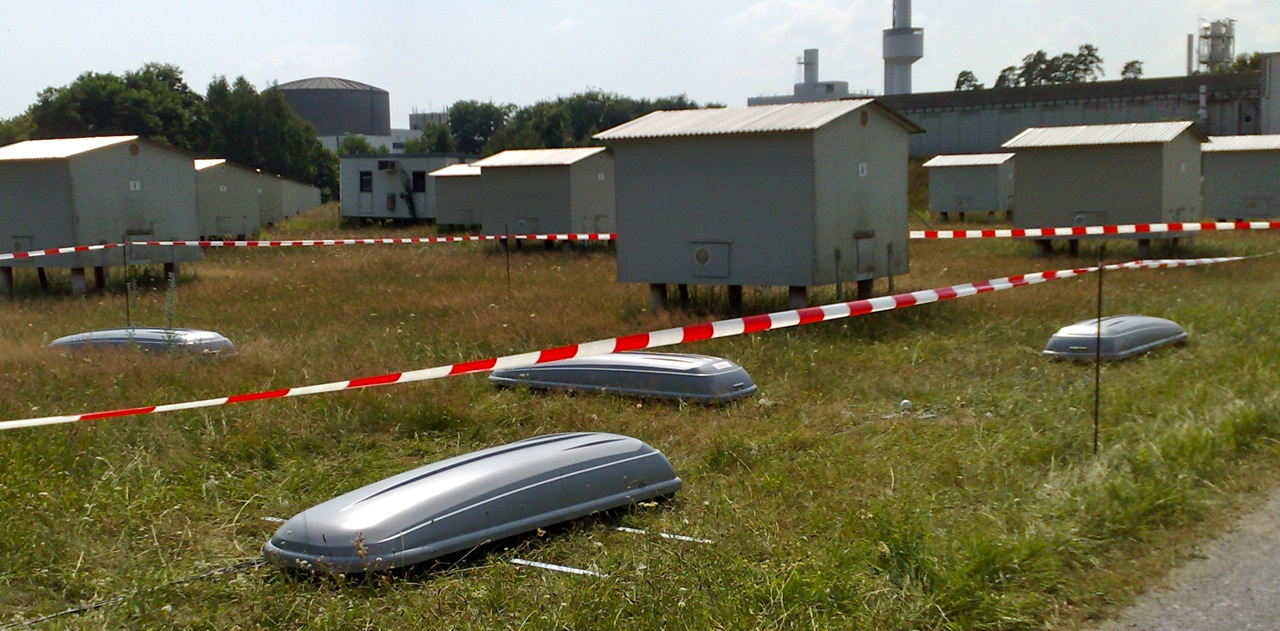
\includegraphics[width=\linewidth]{figures/kascade}
\caption{\hisparc station at the \kascade experiment.  The roof boxes
contain the \hisparc detectors.  Several \kascade detector huts are
visible in the background.  The large building in the background on the
right is the central calorimeter and electronics building.}
\label{fig:kascade-station}
\end{figure}

All detector signals in the same cluster are read out by the \daq electronics.
These electronics are located in a shelter in the center of the cluster. If a
signal goes over threshold, it is temporarily stored in a buffer.
When a preset number of detectors go over threshold, a trigger is generated.
For the inner clusters this number is 20 out of 60 $e/\gamma$ detectors, whereas
for the outer clusters a minimum of 10 out of 32 $e/\gamma$ detectors is
required.  A trigger is distributed throughout the experiment and then the
entire array is read out.  All buffered detector signals are transferred to the
central electronics.  Each detector
signal receives a timestamp from the cluster electronics.  All clocks within the
experiment are synchronized using fiber optic cables, carrying a \SI{1}{\hertz}
and a \SI{5}{\mega\hertz} signal.
The timestamps are generated using these signals at \SI{200}{\nano\second}
accuracy.

Showers are reconstructed in three stages using different algorithms
\cite{Antoni:2000mg}.  First, the shower core position is determined by the
center of gravity of the $e/\gamma$ detector signals.  The shower direction is
determined by assuming a plane shower front.  The shower size (number of
electrons $N_e$ and muons $N_\mu$) is estimated by summing the detector signals
(weighted by a factor which depends on the core distance).  In the next step,
the core position and electron shower size are used as a first guess in a
fitting procedure.  In this procedure, a revised core position and electron
shower size are determined, as well as a shape parameter $s$, by fitting the
lateral distribution function to the detector signals.  The arrival times
(for detectors within a distance of \SI{70}{\meter} from the shower core) are
fitted to a conical shower front.  In the final step the detector signals are adjusted for expected
contributions from other particles, and the fitting procedure is repeated.

Once the shower parameters have been determined, the particle densities can then
be calculated at arbitrary locations and this is used to provide guest
experiments with estimated particle densities at the location of their
detectors. The particle densities are calculated on the shower front, not on the
ground. This is crucial for inclined showers, see \figref{fig:inclined-ldf}.
From the figure, it becomes clear that the core distance $r$ that is being
sampled by a detector is not the distance $r'$ of the detector to the shower
core on the ground.  Furthermore, particles reaching the ground are distributed
over a larger area and thus the density $\rho'$ is lower than the particle
density on the shower front $\rho$. The zenith angle of the shower only has a
small effect on the distribution of particle density on the shower front.

\begin{figure}
\centering
\begin{sansmath}
\pgfmathsetmacro{\unit}{3mm}
\begin{tikzpicture}[x=\unit, y=\unit, draft/.style={red,opacity=0},
                    font=\sffamily,
                    every pin edge/.style={<-, >=stealth', shorten <=2pt}]
\pgfmathsetmacro{\zenith}{30}
\coordinate[label={[draft]below:{$O$}}] (O) at (0, 0);
\begin{scope}
    \clip (-13, -1) rectangle (26, 2);
    \foreach \x in {-32, -31, ..., 33}
        \draw (\x, 0) -- +(225:1);
    \foreach \x in {-32.5, -19.5, ..., 32.5}
        \draw[gray] (\x - 1.2, 0) rectangle (\x + 1.2, 1);
    \draw (-32.5, 0) -- (32.5, 0);
\end{scope}
\coordinate[label={[draft]below:{$S'$}}] (S') at (19.5, 0);
\coordinate[label={[draft]above:{$S_1'$}}] (S1') at ($(S') - (1.2,0)$);
\coordinate[label={[draft]above:{$S_2'$}}] (S2') at ($(S') + (1.2,0)$);
\draw ($(S1') - (0,3pt)$) -- ($(S1') + (0,3pt)$);
\draw ($(S2') - (0,3pt)$) -- ($(S2') + (0,3pt)$);
\draw[dashed] (0, 20) -- (0, -5);
\begin{scope}[rotate=\zenith]
    \coordinate[label={[draft]left:{$A$}}] (A) at (-10, 0);
    \coordinate[label={[draft]right:{$B$}}] (B) at (30, 0);

    \coordinate[label={[draft]above:{$C$}}] (C) at (0, -5);
    \coordinate[label={[draft]below:{$C'$}}] (C') at (0, 25);
    \draw[gray] (C) -- (O);
    \draw (O) -- (C');
    \draw[gray] (A) -- (O);
    \draw (O) -- (B);
    \draw (0, 20pt) arc (90:90-\zenith:20pt);
    \draw (90-.5*\zenith:25pt) node {$\theta$};
    \draw (20pt, 0) arc (0:-\zenith:20pt);
    \draw (-.5*\zenith:25pt) node {$\theta$};

    \coordinate[label={[draft]above:{$S$}}] (S) at ($(A)!(S')!(B)$);
    \coordinate[label={[draft]above:{$S_1$}}] (S1) at ($(A)!(S1')!(B)$);
    \coordinate[label={[draft]above:{$S_2$}}] (S2) at ($(A)!(S2')!(B)$);
    \draw ($(S1) - (0,3pt)$) -- ($(S1) + (0,3pt)$);
    \draw ($(S2) - (0,3pt)$) -- ($(S2) + (0,3pt)$);
\end{scope}
\path (C') -- (C) node[near start, sloped, below] {shower core};
\path (A) -- (B) node[very near end, sloped, below] {shower front};
%\draw[dashed] (S) -- (S');
\draw[dashed] (S1) -- (S1');
\draw[dashed] (S2) -- (S2');
\draw[|<->|] ($(O)!5pt!90:(S)$) -- ($(S)!5pt!-90:(O)$)
    node[midway, sloped, above] {$r$};
\draw[|<->|] ($(O)!10pt!-90:(S')$) -- ($(S')!10pt!90:(O)$)
    node[midway, below] {$r'$ = $r\sec\theta$};
\path (O) -- (S) node[at end, sloped, below] {$\rho$};
%\path (O) -- (S') node[at end, above=-5pt] {$\rho'$};
\node (rho') at ($(S') + (30pt,30pt)$) {$\rho'$ = $\rho\cos\theta$};
\draw[->] (rho') to[bend left=20] (S');

\begin{scope}[rotate=\zenith]
\begin{axis}[x=\unit,height=8cm,ymin=0,ymax=200,xmin=0,xmax=25,axis lines=none,legend style={empty legend, draw=none}]
    \pgfmathsetmacro{\logNe}{5}
    \pgfmathsetmacro{\a}{1.5}
    \pgfmathsetmacro{\b}{3.6}
    \pgfmathsetmacro{\rn}{40}
    \pgfmathsetmacro{\s}{.9}
    \addplot[smooth,id=nkg,domain=.2:20,samples=50] function {10 ** \logNe *
    gamma(\b - \s) / (2 * pi * \rn ** 2 * gamma(\s - \a + 2) * gamma(\a + \b - 2 * \s - 2)) * (x / \rn) ** (\s - \a) * (1 + x / \rn) ** (\s - \b)};
    %\addlegendentry{$\displaystyle\rho(r) = N_e\;\tilde{c}(s) \left(\frac{r}{r_0}\right)^{s - \alpha} \left(1 + \frac{r}{r_0}\right)^{s - \beta}$}
\end{axis}
\end{scope}
\node[pin=above right:{$\rho(r)$}] at (-8, 15) {};
\end{tikzpicture}
\end{sansmath}

\caption{Mapping of the lateral distribution of particle density of an angled
shower to ground level density measurements.  In the figure, $\rho$ and
$\rho'$ illustrate the measurement of the particle density in an area
occupied by a detector.}
\label{fig:inclined-ldf}
\end{figure}

A \hisparc station is installed inside the \kascade array.  The station
consists of four scintillator detectors in the standard triangle setup shown in
\figref{fig:station-layout}. The \kascade cluster in which the \hisparc station
is located will be referred to as the \emph{local cluster}.

The \hisparc station is not used in self-trigger mode. To observe the same
showers, the cluster electronics provide a pulse whenever the \kascade array is
triggered.  This signal is used by the \hisparc electronics to read out the
detectors.  For each trigger, the \hisparc \textsmaller{GPS} receiver provides a
timestamp.
This timestamp is used to synchronize with the \kascade clock. The events
detected by the \hisparc station are reconstructed using the algorithm described
in \chref{ch:reconstruction}. The \kascade array provides estimates of the
particle densities at the location of the \hisparc detectors, as well as the
direction and primary energy of the shower. These measurements are used to
determine the efficiency and accuracy of the reconstruction performed by
\hisparc.


\subsection{Trigger Synchronization}

While \hisparc and \kascade use
different clocks, both clocks derive from the same time standard.  By
determining the offset between the two clocks, the corresponding events in the
datasets can be found.  Note that the \kascade clock expresses time
in UTC, while the \hisparc clock uses GPS time.

The showers in the reconstructed dataset are a subset of the showers seen by the
\kascade array.  In the following, the \hisparc events will be referred to as
\emph{triggered events}, and the dataset provided by \kascade, containing only
reconstructed showers, will be referred to as \emph{reconstructed events}. The
occurence of triggered events follows the Poisson statistics.
In particular, the time differences between consecutive events are independent
random variables which are exponentially distributed.

To determine the clock offset the \hisparc dataset, i.e. the triggered events,
is shifted in time.  For each event, the nearest-neighbor triggered event is
determined.  \figref{fig:timeshifts} shows histograms of the resulting time
differences for various timeshifts. When different events are compared in the
two datasets the resulting time differences are random and determined by the
statistical nature of the triggered events.  The time differences should thus
follow an exponential distribution with rate parameter $\lambda$.  This rate
parameter is not equal to the rate of the triggered events.  Since the procedure
uses nearest neighbors, both preceding and following the reconstructed events,
the mean time differences are halved and the rate parameter is \emph{twice} the
trigger rate.  The figure shows that $\lambda = \SI{7.2}{\hertz}$
which is consistent with the observed trigger rate of \SI{3.6}{\hertz}.

When the timeshift is close to the true offset between the clocks the
correlation shows itself by a spike in the histogram of the time differences,
resulting from correctly synchronized events.  Uncorrelated events with time
differences smaller than the remaining offset will still be selected as
nearest neighbor.  Hence, the data is random and follows Poisson statistics up to the observed spike.
Uncorrelated events with larger time differences will not be selected as the
nearest neighbor.  Thus, the distribution is cut off after the spike.
Optimizing the timeshift results in a single spike.

\figref{fig:timeshifts-corr} shows the residual time differences.  The
distribution on the left has a standard deviation of approximately
\SI{.5}{\micro\second}, which is not yet fully understood but is an unwanted
property of the \kascade hardware \cite{Schieler:2010-clock}.
The shape of this distribution is already visible in a few minutes worth of data
and does not result from changes in the clock offset.  The clock offset slowly
moves back-and-forth over the five-week period with a largest observed deviation
of \SI{8}{\micro\second}.  Since this happens slowly, it is possible to correct
for this shift.  The time difference distribution over the whole period results
from a drifting offset of the \kascade clock hardware.  The offset is stable for
periods of time, and then changes again.

The probability of one or more random triggered events occuring in a time window
of \SI{1}{\micro\second} is \num{7.0e-6}.  Therefore, it can be concluded that
triggered and reconstructed events are correctly synchronized and that the
probability of incorrect matches is very low.

For this particular dataset, the timeshift which results in a mean time
difference closest to zero, is found to be $\overline{t_K - t_H} =
\SI{-13.180}{\second}$.  The time difference between the \hisparc clock
(\textsmaller{GPS}) and the \kascade clock (\textsmaller{UTC}) should be
\SI{14}{\second} due to leap seconds.\footnote{Between January 1, 2006 and
January 1, 2009 the offset between \textsmaller{GPS} and \textsmaller{UTC}
clocks was \SI{14}{\second}, with \textsmaller{UTC} lagging behind
\textsmaller{GPS}.  At the end of December 31, 2008 a leap second was introduced
to bring the offset to \SI{15}{\second}.}  The \SI{820}{\milli\second}
difference is caused by the clock offset in the \kascade experiment
\cite{Schieler:2010-clock}.

\begin{figure}
\centering
% \usepackage{tikz}
% \usetikzlibrary{arrows}
% \usepackage{pgfplots}
% \pgfplotsset{compat=1.3}
% \usepackage[detect-family]{siunitx}
% \usepackage[eulergreek]{sansmath}
% \sisetup{text-sf=\sansmath}
% \usepackage{relsize}
%
\pgfkeysifdefined{/artist/width}
    {\pgfkeysgetvalue{/artist/width}{\defaultwidth}}
    {\def\defaultwidth{ .67\linewidth }}
%
%
\begin{sansmath}
\begin{tikzpicture}[
        font=\sffamily,
        every pin/.style={inner sep=2pt, font={\sffamily\smaller}},
        every label/.style={inner sep=2pt, font={\sffamily\smaller}},
        every pin edge/.style={<-, >=stealth', shorten <=2pt},
        pin distance=2.5ex,
    ]
    \begin{semilogyaxis}[
            width=\defaultwidth,
            %
            title={  },
            %
            xlabel={ Time difference [\si{\second}] },
            ylabel={ Counts },
            %
            xmin={  },
            xmax={  },
            ymin={ 10 },
            ymax={  },
            %
            xtick={  },
            ytick={  },
            %
            tick align=outside,
            max space between ticks=40,
            every tick/.style={},
        ]

        

        
            \addplot[no markers,solid,gray,const plot] coordinates {
                (0.0, 36320)
                (0.01, 34110)
                (0.02, 31606)
                (0.03, 29328)
                (0.04, 27194)
                (0.05, 25462)
                (0.06, 23696)
                (0.07, 21924)
                (0.08, 20594)
                (0.09, 19006)
                (0.1, 17835)
                (0.11, 16675)
                (0.12, 15376)
                (0.13, 14317)
                (0.14, 13424)
                (0.15, 12280)
                (0.16, 11486)
                (0.17, 10725)
                (0.18, 10022)
                (0.19, 9428)
                (0.2, 8809)
                (0.21, 8022)
                (0.22, 7380)
                (0.23, 7052)
                (0.24, 6559)
                (0.25, 6026)
                (0.26, 5613)
                (0.27, 5388)
                (0.28, 5002)
                (0.29, 4642)
                (0.3, 4256)
                (0.31, 3992)
                (0.32, 3580)
                (0.33, 3506)
                (0.34, 3232)
                (0.35, 2870)
                (0.36, 2866)
                (0.37, 2493)
                (0.38, 2454)
                (0.39, 2182)
                (0.4, 2016)
                (0.41, 1950)
                (0.42, 1876)
                (0.43, 1600)
                (0.44, 1599)
                (0.45, 1413)
                (0.46, 1370)
                (0.47, 1274)
                (0.48, 1247)
                (0.49, 1099)
                (0.5, 1035)
                (0.51, 941)
                (0.52, 922)
                (0.53, 861)
                (0.54, 786)
                (0.55, 764)
                (0.56, 701)
                (0.57, 621)
                (0.58, 569)
                (0.59, 554)
                (0.6, 524)
                (0.61, 452)
                (0.62, 437)
                (0.63, 383)
                (0.64, 356)
                (0.65, 322)
                (0.66, 302)
                (0.67, 302)
                (0.68, 269)
                (0.69, 238)
                (0.7, 239)
                (0.71, 225)
                (0.72, 242)
                (0.73, 207)
                (0.74, 187)
                (0.75, 170)
                (0.76, 153)
                (0.77, 155)
                (0.78, 147)
                (0.79, 136)
                (0.8, 135)
                (0.81, 129)
                (0.82, 113)
                (0.83, 101)
                (0.84, 88)
                (0.85, 76)
                (0.86, 74)
                (0.87, 71)
                (0.88, 78)
                (0.89, 55)
                (0.9, 51)
                (0.91, 45)
                (0.92, 41)
                (0.93, 50)
                (0.94, 53)
                (0.95, 41)
                (0.96, 38)
                (0.97, 31)
                (0.98, 28)
                (0.99, 25)
                (1.0, 25)
            };
        
            \addplot[no markers,dashed,gray,const plot] coordinates {
                (0.0, 36423)
                (0.01, 33614)
                (0.02, 31628)
                (0.03, 28948)
                (0.04, 27340)
                (0.05, 25289)
                (0.06, 23755)
                (0.07, 22026)
                (0.08, 20419)
                (0.09, 18782)
                (0.1, 17863)
                (0.11, 16471)
                (0.12, 15486)
                (0.13, 14120)
                (0.14, 13321)
                (0.15, 12526)
                (0.16, 11607)
                (0.17, 10663)
                (0.18, 146869)
                (0.19, 1e-99)
                (0.2, 1e-99)
                (0.21, 1e-99)
                (0.22, 1e-99)
                (0.23, 1e-99)
                (0.24, 1e-99)
                (0.25, 1e-99)
                (0.26, 1e-99)
                (0.27, 1e-99)
                (0.28, 1e-99)
                (0.29, 1)
                (0.3, 1e-99)
                (0.31, 1e-99)
                (0.32, 1e-99)
                (0.33, 1e-99)
                (0.34, 1e-99)
                (0.35, 1e-99)
                (0.36, 1e-99)
                (0.37, 1e-99)
                (0.38, 1e-99)
                (0.39, 1e-99)
                (0.4, 1e-99)
                (0.41, 1e-99)
                (0.42, 1e-99)
                (0.43, 1e-99)
                (0.44, 1e-99)
                (0.45, 1e-99)
                (0.46, 1e-99)
                (0.47, 1e-99)
                (0.48, 1e-99)
                (0.49, 1e-99)
                (0.5, 1)
                (0.51, 1e-99)
                (0.52, 1)
                (0.53, 1e-99)
                (0.54, 1e-99)
                (0.55, 1e-99)
                (0.56, 1e-99)
                (0.57, 1e-99)
                (0.58, 1e-99)
                (0.59, 1e-99)
                (0.6, 1e-99)
                (0.61, 1e-99)
                (0.62, 1e-99)
                (0.63, 1e-99)
                (0.64, 1e-99)
                (0.65, 1e-99)
                (0.66, 1)
                (0.67, 1e-99)
                (0.68, 1e-99)
                (0.69, 1e-99)
                (0.7, 1e-99)
                (0.71, 1e-99)
                (0.72, 1)
                (0.73, 1e-99)
                (0.74, 1e-99)
                (0.75, 1e-99)
                (0.76, 1e-99)
                (0.77, 1e-99)
                (0.78, 1e-99)
                (0.79, 1e-99)
                (0.8, 1e-99)
                (0.81, 1e-99)
                (0.82, 1)
                (0.83, 1e-99)
                (0.84, 1)
                (0.85, 1e-99)
                (0.86, 1e-99)
                (0.87, 1e-99)
                (0.88, 1)
                (0.89, 1e-99)
                (0.9, 1e-99)
                (0.91, 1e-99)
                (0.92, 1e-99)
                (0.93, 1e-99)
                (0.94, 1e-99)
                (0.95, 1e-99)
                (0.96, 1e-99)
                (0.97, 1e-99)
                (0.98, 1e-99)
                (0.99, 1e-99)
                (1.0, 1e-99)
            };
        
            \addplot[no markers,dashdotted,gray,const plot] coordinates {
                (0.0, 36200)
                (0.01, 33880)
                (0.02, 31679)
                (0.03, 29464)
                (0.04, 27477)
                (0.05, 25317)
                (0.06, 23721)
                (0.07, 21973)
                (0.08, 20488)
                (0.09, 19047)
                (0.1, 17666)
                (0.11, 16501)
                (0.12, 15313)
                (0.13, 14373)
                (0.14, 13427)
                (0.15, 12487)
                (0.16, 11530)
                (0.17, 10689)
                (0.18, 10184)
                (0.19, 9352)
                (0.2, 8544)
                (0.21, 8122)
                (0.22, 7599)
                (0.23, 7153)
                (0.24, 6464)
                (0.25, 6085)
                (0.26, 5727)
                (0.27, 5260)
                (0.28, 4897)
                (0.29, 4525)
                (0.3, 4229)
                (0.31, 3920)
                (0.32, 3672)
                (0.33, 3514)
                (0.34, 3171)
                (0.35, 3008)
                (0.36, 2749)
                (0.37, 2634)
                (0.38, 2400)
                (0.39, 2197)
                (0.4, 2102)
                (0.41, 1932)
                (0.42, 1759)
                (0.43, 1675)
                (0.44, 1517)
                (0.45, 1502)
                (0.46, 1404)
                (0.47, 1288)
                (0.48, 1159)
                (0.49, 1132)
                (0.5, 1013)
                (0.51, 929)
                (0.52, 891)
                (0.53, 829)
                (0.54, 773)
                (0.55, 684)
                (0.56, 647)
                (0.57, 609)
                (0.58, 629)
                (0.59, 522)
                (0.6, 521)
                (0.61, 455)
                (0.62, 424)
                (0.63, 421)
                (0.64, 364)
                (0.65, 358)
                (0.66, 336)
                (0.67, 344)
                (0.68, 291)
                (0.69, 298)
                (0.7, 236)
                (0.71, 237)
                (0.72, 217)
                (0.73, 183)
                (0.74, 183)
                (0.75, 180)
                (0.76, 180)
                (0.77, 181)
                (0.78, 146)
                (0.79, 128)
                (0.8, 125)
                (0.81, 1713)
                (0.82, 1e-99)
                (0.83, 1e-99)
                (0.84, 1e-99)
                (0.85, 1e-99)
                (0.86, 1e-99)
                (0.87, 1e-99)
                (0.88, 1e-99)
                (0.89, 1e-99)
                (0.9, 1e-99)
                (0.91, 1e-99)
                (0.92, 1e-99)
                (0.93, 1e-99)
                (0.94, 1e-99)
                (0.95, 1e-99)
                (0.96, 1e-99)
                (0.97, 1e-99)
                (0.98, 1e-99)
                (0.99, 1e-99)
                (1.0, 1e-99)
            };
        
            \addplot[no markers,solid] coordinates {
                (0.005, 36401.902475)
                (0.015, 33886.1633767)
                (0.025, 31544.2872575)
                (0.035, 29364.2584297)
                (0.045, 27334.8916109)
                (0.055, 25445.7745347)
                (0.065, 23687.2145273)
                (0.075, 22050.1887769)
                (0.085, 20526.2980388)
                (0.095, 19107.7235411)
                (0.105, 17787.1868679)
                (0.115, 16557.9126155)
                (0.125, 15413.5936288)
                (0.135, 14348.358641)
                (0.145, 13356.7421492)
                (0.155, 12433.6563716)
                (0.165, 11574.3651439)
                (0.175, 10774.4596183)
                (0.185, 10029.8356432)
                (0.195, 9336.67270493)
                (0.205, 8691.41432625)
                (0.215, 8090.74981826)
                (0.225, 7531.59729412)
                (0.235, 7011.08785651)
                (0.245, 6526.55087786)
                (0.255, 6075.50029797)
                (0.265, 5655.62186849)
                (0.275, 5264.761279)
                (0.285, 4900.91310371)
                (0.295, 4562.21051197)
                (0.305, 4246.91569002)
                (0.315, 3953.41092455)
                (0.325, 3680.1903026)
                (0.335, 3425.85198498)
                (0.345, 3189.09101378)
                (0.355, 2968.69261683)
                (0.365, 2763.525975)
                (0.375, 2572.53842018)
                (0.385, 2394.75003426)
                (0.395, 2229.24862136)
                (0.405, 2075.18502756)
                (0.415, 1931.76878403)
                (0.425, 1798.26405136)
                (0.435, 1673.98584402)
                (0.445, 1558.29651595)
                (0.455, 1450.60248885)
                (0.465, 1350.35120666)
                (0.475, 1257.02830054)
                (0.485, 1170.15494975)
                (0.495, 1089.28542486)
                (0.505, 1014.00480088)
                (0.515, 943.926828298)
                (0.525, 878.69195137)
                (0.535, 817.965463271)
                (0.545, 761.435788801)
                (0.555, 708.812885752)
                (0.565, 659.826756764)
                (0.575, 614.226064019)
                (0.585, 571.776839682)
                (0.595, 532.261285459)
                (0.605, 495.476655115)
                (0.615, 461.234214231)
                (0.625, 429.35827184)
                (0.635, 399.685278996)
                (0.645, 372.062989637)
                (0.655, 346.349679441)
                (0.665, 322.413418669)
                (0.675, 300.131395258)
                (0.685, 279.389284699)
                (0.695, 260.080663463)
                (0.705, 242.10646296)
                (0.715, 225.37446124)
                (0.725, 209.798809822)
                (0.735, 195.299593222)
                (0.745, 181.802418922)
                (0.755, 169.23803568)
                (0.765, 157.541978212)
                (0.775, 146.654236438)
                (0.785, 136.518947581)
                (0.795, 127.084109544)
                (0.805, 118.301314102)
                (0.815, 110.125498525)
                (0.825, 102.514714376)
                (0.835, 95.4299122759)
                (0.845, 88.834741553)
                (0.855, 82.6953637343)
                (0.865, 76.980278927)
                (0.875, 71.6601641987)
                (0.885, 66.7077231281)
                (0.895, 62.0975457521)
                (0.905, 57.8059781929)
                (0.915, 53.8110012942)
                (0.925, 50.0921176461)
                (0.935, 46.6302464166)
                (0.945, 43.4076254518)
                (0.955, 40.4077201422)
                (0.965, 37.6151385868)
                (0.975, 35.0155526202)
                (0.985, 32.5956242981)
                (0.995, 30.342937463)
            };
        

        

        

        
    \end{semilogyaxis}
\end{tikzpicture}
\end{sansmath}
\caption{The triggered data (\hisparc clock) is shifted in time to
synchronize with the reconstructed data (\kascade clock).  For each
reconstructed event, the time difference with the nearest triggered event
is determined.  The time shifts are \SI{-12}{\second} (solid gray line),
\SI{-13}{\second} (dashed gray line) and \SI{-14}{\second} (dashdotted
gray line).  For uncorrelated events, the time differences follow Poisson
statistics and hence give rise to an exponential distribution.  The slope
of the distribution is \SI{7.2}{\hertz} (solid black line), which is equal
to twice the observed trigger rate of \SI{3.6}{\hertz}.  If the time shift
differs only slightly from the clock offset, partial matches give rise to
spikes in the graph.  These occur at the residual time difference to the
correct clock offset.  In that case, for each reconstructed event, there
is a triggered event at precisely this time difference.  There are
uncorrelated events randomly occuring with smaller time differences,
resulting in an exponential distribution up to the spike.}
\label{fig:timeshifts}
\end{figure}

\begin{figure}
\centering
{\pgfkeys{/artist/width/.initial=.45\linewidth}
% \usepackage{tikz}
% \usetikzlibrary{arrows,pgfplots.groupplots}
% \usepackage{pgfplots}
% \pgfplotsset{compat=1.3}
% \usepackage[detect-family]{siunitx}
% \usepackage[eulergreek]{sansmath}
% \sisetup{text-sf=\sansmath}
% \usepackage{relsize}
%
\pgfkeysifdefined{/artist/width}
    {\pgfkeysgetvalue{/artist/width}{\defaultwidth}}
    {\def\defaultwidth{ .45\linewidth }}
%
%
\begin{sansmath}
\begin{tikzpicture}[font=\sffamily]
\node[inner sep=0pt] (plot) {
    \begin{tikzpicture}[
            inner sep=.3333em,
            font=\sffamily,
            every pin/.style={inner sep=2pt, font={\sffamily\smaller}},
            every label/.style={inner sep=2pt, font={\sffamily\smaller}},
            every pin edge/.style={<-, >=stealth', shorten <=2pt},
            pin distance=2.5ex,
        ]
        \begin{groupplot}[
                xmode=normal,
                ymode=normal,
                width=\defaultwidth,
                %
                xmin={  },
                xmax={  },
                ymin={ 0 },
                ymax={  },
                %
                group style={rows=1,columns=2,
                             horizontal sep=4pt, vertical sep=4pt},
                %
                tick align=outside,
                max space between ticks=40,
                every tick/.style={},
                axis on top,
                %
                xtick=\empty, ytick=\empty,
                scaled ticks=false,
            ]
            
                
                \nextgroupplot[
                    % Default: empty ticks all round the border of the
                    % multiplot
                            xtick={  },
                            xtick pos=both,
                            xticklabel=\empty,
                            ytick={  },
                            ytick pos=left,
                            yticklabel=\empty,
                        xticklabel={},
                        yticklabel={},
                    title={ Jul 2, 2008 },
                    xlabel={  },
                    ylabel={  },
                ]

                

                

                
                    \addplot[no markers,solid,const plot] coordinates {
                        (-8.0, 0)
                        (-7.99, 0)
                        (-7.98, 0)
                        (-7.97, 0)
                        (-7.96, 0)
                        (-7.95, 0)
                        (-7.94, 0)
                        (-7.93, 0)
                        (-7.92, 0)
                        (-7.91, 0)
                        (-7.9, 0)
                        (-7.89, 0)
                        (-7.88, 0)
                        (-7.87, 0)
                        (-7.86, 0)
                        (-7.85, 0)
                        (-7.84, 0)
                        (-7.83, 0)
                        (-7.82, 0)
                        (-7.81, 0)
                        (-7.8, 0)
                        (-7.79, 0)
                        (-7.78, 3)
                        (-7.77, 7)
                        (-7.76, 26)
                        (-7.75, 31)
                        (-7.74, 40)
                        (-7.73, 56)
                        (-7.72, 73)
                        (-7.71, 91)
                        (-7.7, 94)
                        (-7.69, 107)
                        (-7.68, 115)
                        (-7.67, 138)
                        (-7.66, 130)
                        (-7.65, 184)
                        (-7.64, 161)
                        (-7.63, 224)
                        (-7.62, 244)
                        (-7.61, 227)
                        (-7.6, 236)
                        (-7.59, 281)
                        (-7.58, 277)
                        (-7.57, 271)
                        (-7.56, 306)
                        (-7.55, 304)
                        (-7.54, 323)
                        (-7.53, 329)
                        (-7.52, 302)
                        (-7.51, 334)
                        (-7.5, 304)
                        (-7.49, 323)
                        (-7.48, 321)
                        (-7.47, 340)
                        (-7.46, 311)
                        (-7.45, 340)
                        (-7.44, 322)
                        (-7.43, 320)
                        (-7.42, 342)
                        (-7.41, 336)
                        (-7.4, 321)
                        (-7.39, 368)
                        (-7.38, 312)
                        (-7.37, 335)
                        (-7.36, 309)
                        (-7.35, 346)
                        (-7.34, 342)
                        (-7.33, 346)
                        (-7.32, 371)
                        (-7.31, 339)
                        (-7.3, 348)
                        (-7.29, 394)
                        (-7.28, 378)
                        (-7.27, 375)
                        (-7.26, 382)
                        (-7.25, 365)
                        (-7.24, 393)
                        (-7.23, 419)
                        (-7.22, 366)
                        (-7.21, 369)
                        (-7.2, 370)
                        (-7.19, 358)
                        (-7.18, 342)
                        (-7.17, 332)
                        (-7.16, 285)
                        (-7.15, 300)
                        (-7.14, 296)
                        (-7.13, 323)
                        (-7.12, 274)
                        (-7.11, 231)
                        (-7.1, 234)
                        (-7.09, 212)
                        (-7.08, 210)
                        (-7.07, 194)
                        (-7.06, 179)
                        (-7.05, 159)
                        (-7.04, 160)
                        (-7.03, 160)
                        (-7.02, 155)
                        (-7.01, 113)
                        (-7.0, 117)
                        (-6.99, 107)
                        (-6.98, 119)
                        (-6.97, 100)
                        (-6.96, 97)
                        (-6.95, 87)
                        (-6.94, 79)
                        (-6.93, 73)
                        (-6.92, 77)
                        (-6.91, 73)
                        (-6.9, 55)
                        (-6.89, 54)
                        (-6.88, 33)
                        (-6.87, 54)
                        (-6.86, 42)
                        (-6.85, 41)
                        (-6.84, 34)
                        (-6.83, 28)
                        (-6.82, 17)
                        (-6.81, 17)
                        (-6.8, 16)
                        (-6.79, 18)
                        (-6.78, 17)
                        (-6.77, 6)
                        (-6.76, 11)
                        (-6.75, 9)
                        (-6.74, 6)
                        (-6.73, 9)
                        (-6.72, 6)
                        (-6.71, 1)
                        (-6.7, 3)
                        (-6.69, 3)
                        (-6.68, 3)
                        (-6.67, 0)
                        (-6.66, 3)
                        (-6.65, 0)
                        (-6.64, 2)
                        (-6.63, 2)
                        (-6.62, 2)
                        (-6.61, 0)
                        (-6.6, 0)
                        (-6.59, 0)
                        (-6.58, 0)
                        (-6.57, 1)
                        (-6.56, 0)
                        (-6.55, 2)
                        (-6.54, 0)
                        (-6.53, 2)
                        (-6.52, 1)
                        (-6.51, 0)
                        (-6.5, 0)
                        (-6.49, 2)
                        (-6.48, 0)
                        (-6.47, 0)
                        (-6.46, 2)
                        (-6.45, 2)
                        (-6.44, 1)
                        (-6.43, 0)
                        (-6.42, 0)
                        (-6.41, 0)
                        (-6.4, 1)
                        (-6.39, 2)
                        (-6.38, 0)
                        (-6.37, 2)
                        (-6.36, 0)
                        (-6.35, 0)
                        (-6.34, 0)
                        (-6.33, 0)
                        (-6.32, 0)
                        (-6.31, 0)
                        (-6.3, 1)
                        (-6.29, 0)
                        (-6.28, 0)
                        (-6.27, 0)
                        (-6.26, 1)
                        (-6.25, 0)
                        (-6.24, 0)
                        (-6.23, 1)
                        (-6.22, 0)
                        (-6.21, 0)
                        (-6.2, 1)
                        (-6.19, 0)
                        (-6.18, 0)
                        (-6.17, 0)
                        (-6.16, 0)
                        (-6.15, 2)
                        (-6.14, 0)
                        (-6.13, 0)
                        (-6.12, 0)
                        (-6.11, 0)
                        (-6.1, 0)
                        (-6.09, 0)
                        (-6.08, 0)
                        (-6.07, 0)
                        (-6.06, 0)
                        (-6.05, 0)
                        (-6.04, 0)
                        (-6.03, 1)
                        (-6.02, 0)
                        (-6.01, 0)
                    };
                

                

                

                

                

            
                
                \nextgroupplot[
                    % Default: empty ticks all round the border of the
                    % multiplot
                            xtick={  },
                            xtick pos=both,
                            xticklabel=\empty,
                            ytick={  },
                            ytick pos=right,
                            yticklabel=\empty,
                        xticklabel={},
                        yticklabel={},
                    title={ Jul 1 - Aug 6, 2008 },
                    xlabel={  },
                    ylabel={  },
                ]

                

                

                
                    \addplot[no markers,solid,const plot] coordinates {
                        (-10.0, 0)
                        (-9.99, 0)
                        (-9.98, 0)
                        (-9.97, 0)
                        (-9.96, 0)
                        (-9.95, 0)
                        (-9.94, 0)
                        (-9.93, 0)
                        (-9.92, 0)
                        (-9.91, 0)
                        (-9.9, 0)
                        (-9.89, 0)
                        (-9.88, 0)
                        (-9.87, 0)
                        (-9.86, 0)
                        (-9.85, 0)
                        (-9.84, 0)
                        (-9.83, 0)
                        (-9.82, 0)
                        (-9.81, 0)
                        (-9.8, 0)
                        (-9.79, 0)
                        (-9.78, 0)
                        (-9.77, 0)
                        (-9.76, 0)
                        (-9.75, 0)
                        (-9.74, 0)
                        (-9.73, 0)
                        (-9.72, 0)
                        (-9.71, 0)
                        (-9.7, 0)
                        (-9.69, 0)
                        (-9.68, 0)
                        (-9.67, 0)
                        (-9.66, 0)
                        (-9.65, 0)
                        (-9.64, 0)
                        (-9.63, 0)
                        (-9.62, 0)
                        (-9.61, 0)
                        (-9.6, 0)
                        (-9.59, 0)
                        (-9.58, 0)
                        (-9.57, 0)
                        (-9.56, 0)
                        (-9.55, 0)
                        (-9.54, 0)
                        (-9.53, 0)
                        (-9.52, 0)
                        (-9.51, 0)
                        (-9.5, 0)
                        (-9.49, 0)
                        (-9.48, 0)
                        (-9.47, 0)
                        (-9.46, 0)
                        (-9.45, 0)
                        (-9.44, 0)
                        (-9.43, 0)
                        (-9.42, 0)
                        (-9.41, 0)
                        (-9.4, 0)
                        (-9.39, 0)
                        (-9.38, 0)
                        (-9.37, 0)
                        (-9.36, 0)
                        (-9.35, 0)
                        (-9.34, 0)
                        (-9.33, 0)
                        (-9.32, 0)
                        (-9.31, 0)
                        (-9.3, 0)
                        (-9.29, 0)
                        (-9.28, 0)
                        (-9.27, 0)
                        (-9.26, 0)
                        (-9.25, 0)
                        (-9.24, 0)
                        (-9.23, 0)
                        (-9.22, 0)
                        (-9.21, 0)
                        (-9.2, 0)
                        (-9.19, 0)
                        (-9.18, 0)
                        (-9.17, 0)
                        (-9.16, 0)
                        (-9.15, 0)
                        (-9.14, 0)
                        (-9.13, 0)
                        (-9.12, 0)
                        (-9.11, 0)
                        (-9.1, 0)
                        (-9.09, 0)
                        (-9.08, 0)
                        (-9.07, 0)
                        (-9.06, 0)
                        (-9.05, 0)
                        (-9.04, 0)
                        (-9.03, 0)
                        (-9.02, 0)
                        (-9.01, 0)
                        (-9.0, 0)
                        (-8.99, 0)
                        (-8.98, 0)
                        (-8.97, 0)
                        (-8.96, 0)
                        (-8.95, 0)
                        (-8.94, 0)
                        (-8.93, 0)
                        (-8.92, 0)
                        (-8.91, 0)
                        (-8.9, 0)
                        (-8.89, 0)
                        (-8.88, 0)
                        (-8.87, 0)
                        (-8.86, 0)
                        (-8.85, 0)
                        (-8.84, 0)
                        (-8.83, 0)
                        (-8.82, 0)
                        (-8.81, 0)
                        (-8.8, 0)
                        (-8.79, 0)
                        (-8.78, 0)
                        (-8.77, 0)
                        (-8.76, 0)
                        (-8.75, 0)
                        (-8.74, 0)
                        (-8.73, 0)
                        (-8.72, 0)
                        (-8.71, 0)
                        (-8.7, 0)
                        (-8.69, 0)
                        (-8.68, 0)
                        (-8.67, 0)
                        (-8.66, 0)
                        (-8.65, 0)
                        (-8.64, 0)
                        (-8.63, 0)
                        (-8.62, 0)
                        (-8.61, 0)
                        (-8.6, 0)
                        (-8.59, 0)
                        (-8.58, 0)
                        (-8.57, 0)
                        (-8.56, 0)
                        (-8.55, 0)
                        (-8.54, 0)
                        (-8.53, 0)
                        (-8.52, 0)
                        (-8.51, 0)
                        (-8.5, 0)
                        (-8.49, 0)
                        (-8.48, 0)
                        (-8.47, 0)
                        (-8.46, 0)
                        (-8.45, 0)
                        (-8.44, 0)
                        (-8.43, 0)
                        (-8.42, 0)
                        (-8.41, 0)
                        (-8.4, 0)
                        (-8.39, 0)
                        (-8.38, 0)
                        (-8.37, 0)
                        (-8.36, 0)
                        (-8.35, 0)
                        (-8.34, 0)
                        (-8.33, 0)
                        (-8.32, 0)
                        (-8.31, 0)
                        (-8.3, 0)
                        (-8.29, 0)
                        (-8.28, 0)
                        (-8.27, 0)
                        (-8.26, 0)
                        (-8.25, 0)
                        (-8.24, 0)
                        (-8.23, 0)
                        (-8.22, 0)
                        (-8.21, 0)
                        (-8.2, 0)
                        (-8.19, 0)
                        (-8.18, 0)
                        (-8.17, 0)
                        (-8.16, 0)
                        (-8.15, 0)
                        (-8.14, 0)
                        (-8.13, 0)
                        (-8.12, 0)
                        (-8.11, 0)
                        (-8.1, 0)
                        (-8.09, 1)
                        (-8.08, 4)
                        (-8.07, 10)
                        (-8.06, 16)
                        (-8.05, 19)
                        (-8.04, 25)
                        (-8.03, 31)
                        (-8.02, 35)
                        (-8.01, 41)
                        (-8.0, 58)
                        (-7.99, 44)
                        (-7.98, 54)
                        (-7.97, 70)
                        (-7.96, 64)
                        (-7.95, 77)
                        (-7.94, 106)
                        (-7.93, 118)
                        (-7.92, 133)
                        (-7.91, 159)
                        (-7.9, 177)
                        (-7.89, 179)
                        (-7.88, 151)
                        (-7.87, 212)
                        (-7.86, 227)
                        (-7.85, 223)
                        (-7.84, 220)
                        (-7.83, 242)
                        (-7.82, 233)
                        (-7.81, 245)
                        (-7.8, 272)
                        (-7.79, 273)
                        (-7.78, 332)
                        (-7.77, 316)
                        (-7.76, 360)
                        (-7.75, 344)
                        (-7.74, 417)
                        (-7.73, 450)
                        (-7.72, 469)
                        (-7.71, 520)
                        (-7.7, 537)
                        (-7.69, 539)
                        (-7.68, 617)
                        (-7.67, 641)
                        (-7.66, 645)
                        (-7.65, 723)
                        (-7.64, 780)
                        (-7.63, 807)
                        (-7.62, 900)
                        (-7.61, 881)
                        (-7.6, 921)
                        (-7.59, 981)
                        (-7.58, 979)
                        (-7.57, 993)
                        (-7.56, 1095)
                        (-7.55, 1050)
                        (-7.54, 1171)
                        (-7.53, 1132)
                        (-7.52, 1125)
                        (-7.51, 1151)
                        (-7.5, 1099)
                        (-7.49, 1155)
                        (-7.48, 1114)
                        (-7.47, 1166)
                        (-7.46, 1027)
                        (-7.45, 1159)
                        (-7.44, 1113)
                        (-7.43, 1141)
                        (-7.42, 1072)
                        (-7.41, 1154)
                        (-7.4, 1104)
                        (-7.39, 1239)
                        (-7.38, 1136)
                        (-7.37, 1156)
                        (-7.36, 1109)
                        (-7.35, 1229)
                        (-7.34, 1186)
                        (-7.33, 1245)
                        (-7.32, 1244)
                        (-7.31, 1225)
                        (-7.3, 1227)
                        (-7.29, 1303)
                        (-7.28, 1329)
                        (-7.27, 1343)
                        (-7.26, 1315)
                        (-7.25, 1328)
                        (-7.24, 1311)
                        (-7.23, 1379)
                        (-7.22, 1360)
                        (-7.21, 1348)
                        (-7.2, 1376)
                        (-7.19, 1349)
                        (-7.18, 1300)
                        (-7.17, 1268)
                        (-7.16, 1271)
                        (-7.15, 1275)
                        (-7.14, 1302)
                        (-7.13, 1283)
                        (-7.12, 1192)
                        (-7.11, 1188)
                        (-7.1, 1178)
                        (-7.09, 1228)
                        (-7.08, 1180)
                        (-7.07, 1182)
                        (-7.06, 1115)
                        (-7.05, 1124)
                        (-7.04, 1127)
                        (-7.03, 1111)
                        (-7.02, 1199)
                        (-7.01, 1094)
                        (-7.0, 1093)
                        (-6.99, 1155)
                        (-6.98, 1102)
                        (-6.97, 1105)
                        (-6.96, 1105)
                        (-6.95, 1146)
                        (-6.94, 1123)
                        (-6.93, 1192)
                        (-6.92, 1158)
                        (-6.91, 1157)
                        (-6.9, 1168)
                        (-6.89, 1131)
                        (-6.88, 1176)
                        (-6.87, 1154)
                        (-6.86, 1154)
                        (-6.85, 1185)
                        (-6.84, 1187)
                        (-6.83, 1110)
                        (-6.82, 1111)
                        (-6.81, 1130)
                        (-6.8, 1173)
                        (-6.79, 1123)
                        (-6.78, 1167)
                        (-6.77, 1165)
                        (-6.76, 1148)
                        (-6.75, 1100)
                        (-6.74, 1092)
                        (-6.73, 1098)
                        (-6.72, 1092)
                        (-6.71, 1157)
                        (-6.7, 1077)
                        (-6.69, 1047)
                        (-6.68, 1016)
                        (-6.67, 1065)
                        (-6.66, 1130)
                        (-6.65, 1045)
                        (-6.64, 1070)
                        (-6.63, 1114)
                        (-6.62, 1042)
                        (-6.61, 1061)
                        (-6.6, 1038)
                        (-6.59, 1069)
                        (-6.58, 1062)
                        (-6.57, 1005)
                        (-6.56, 1002)
                        (-6.55, 1050)
                        (-6.54, 1063)
                        (-6.53, 1035)
                        (-6.52, 1011)
                        (-6.51, 987)
                        (-6.5, 1023)
                        (-6.49, 999)
                        (-6.48, 979)
                        (-6.47, 966)
                        (-6.46, 990)
                        (-6.45, 1046)
                        (-6.44, 948)
                        (-6.43, 994)
                        (-6.42, 941)
                        (-6.41, 906)
                        (-6.4, 925)
                        (-6.39, 889)
                        (-6.38, 917)
                        (-6.37, 894)
                        (-6.36, 858)
                        (-6.35, 906)
                        (-6.34, 827)
                        (-6.33, 855)
                        (-6.32, 814)
                        (-6.31, 780)
                        (-6.3, 830)
                        (-6.29, 782)
                        (-6.28, 808)
                        (-6.27, 830)
                        (-6.26, 818)
                        (-6.25, 770)
                        (-6.24, 785)
                        (-6.23, 798)
                        (-6.22, 745)
                        (-6.21, 736)
                        (-6.2, 811)
                        (-6.19, 705)
                        (-6.18, 736)
                        (-6.17, 722)
                        (-6.16, 715)
                        (-6.15, 742)
                        (-6.14, 752)
                        (-6.13, 683)
                        (-6.12, 714)
                        (-6.11, 731)
                        (-6.1, 662)
                        (-6.09, 671)
                        (-6.08, 656)
                        (-6.07, 668)
                        (-6.06, 669)
                        (-6.05, 661)
                        (-6.04, 689)
                        (-6.03, 638)
                        (-6.02, 649)
                        (-6.01, 650)
                        (-6.0, 680)
                        (-5.99, 659)
                        (-5.98, 676)
                        (-5.97, 648)
                        (-5.96, 613)
                        (-5.95, 641)
                        (-5.94, 636)
                        (-5.93, 655)
                        (-5.92, 618)
                        (-5.91, 575)
                        (-5.9, 618)
                        (-5.89, 665)
                        (-5.88, 676)
                        (-5.87, 566)
                        (-5.86, 639)
                        (-5.85, 590)
                        (-5.84, 609)
                        (-5.83, 583)
                        (-5.82, 593)
                        (-5.81, 561)
                        (-5.8, 602)
                        (-5.79, 552)
                        (-5.78, 562)
                        (-5.77, 535)
                        (-5.76, 542)
                        (-5.75, 474)
                        (-5.74, 530)
                        (-5.73, 501)
                        (-5.72, 526)
                        (-5.71, 484)
                        (-5.7, 466)
                        (-5.69, 512)
                        (-5.68, 493)
                        (-5.67, 468)
                        (-5.66, 485)
                        (-5.65, 519)
                        (-5.64, 510)
                        (-5.63, 457)
                        (-5.62, 481)
                        (-5.61, 527)
                        (-5.6, 527)
                        (-5.59, 524)
                        (-5.58, 491)
                        (-5.57, 517)
                        (-5.56, 518)
                        (-5.55, 549)
                        (-5.54, 535)
                        (-5.53, 469)
                        (-5.52, 484)
                        (-5.51, 511)
                        (-5.5, 531)
                        (-5.49, 518)
                        (-5.48, 511)
                        (-5.47, 517)
                        (-5.46, 532)
                        (-5.45, 515)
                        (-5.44, 525)
                        (-5.43, 534)
                        (-5.42, 496)
                        (-5.41, 530)
                        (-5.4, 541)
                        (-5.39, 520)
                        (-5.38, 550)
                        (-5.37, 520)
                        (-5.36, 535)
                        (-5.35, 538)
                        (-5.34, 557)
                        (-5.33, 516)
                        (-5.32, 560)
                        (-5.31, 531)
                        (-5.3, 513)
                        (-5.29, 506)
                        (-5.28, 506)
                        (-5.27, 573)
                        (-5.26, 508)
                        (-5.25, 537)
                        (-5.24, 550)
                        (-5.23, 525)
                        (-5.22, 470)
                        (-5.21, 524)
                        (-5.2, 526)
                        (-5.19, 520)
                        (-5.18, 547)
                        (-5.17, 503)
                        (-5.16, 524)
                        (-5.15, 548)
                        (-5.14, 499)
                        (-5.13, 489)
                        (-5.12, 448)
                        (-5.11, 487)
                        (-5.1, 503)
                        (-5.09, 495)
                        (-5.08, 466)
                        (-5.07, 484)
                        (-5.06, 531)
                        (-5.05, 456)
                        (-5.04, 448)
                        (-5.03, 473)
                        (-5.02, 450)
                        (-5.01, 463)
                        (-5.0, 413)
                        (-4.99, 392)
                        (-4.98, 360)
                        (-4.97, 381)
                        (-4.96, 395)
                        (-4.95, 400)
                        (-4.94, 336)
                        (-4.93, 311)
                        (-4.92, 325)
                        (-4.91, 346)
                        (-4.9, 331)
                        (-4.89, 326)
                        (-4.88, 321)
                        (-4.87, 286)
                        (-4.86, 260)
                        (-4.85, 291)
                        (-4.84, 282)
                        (-4.83, 331)
                        (-4.82, 269)
                        (-4.81, 241)
                        (-4.8, 268)
                        (-4.79, 245)
                        (-4.78, 251)
                        (-4.77, 238)
                        (-4.76, 239)
                        (-4.75, 209)
                        (-4.74, 245)
                        (-4.73, 254)
                        (-4.72, 268)
                        (-4.71, 208)
                        (-4.7, 240)
                        (-4.69, 223)
                        (-4.68, 240)
                        (-4.67, 214)
                        (-4.66, 227)
                        (-4.65, 191)
                        (-4.64, 201)
                        (-4.63, 229)
                        (-4.62, 196)
                        (-4.61, 215)
                        (-4.6, 247)
                        (-4.59, 205)
                        (-4.58, 234)
                        (-4.57, 240)
                        (-4.56, 207)
                        (-4.55, 230)
                        (-4.54, 227)
                        (-4.53, 204)
                        (-4.52, 226)
                        (-4.51, 250)
                        (-4.5, 257)
                        (-4.49, 261)
                        (-4.48, 226)
                        (-4.47, 290)
                        (-4.46, 266)
                        (-4.45, 299)
                        (-4.44, 278)
                        (-4.43, 294)
                        (-4.42, 274)
                        (-4.41, 328)
                        (-4.4, 333)
                        (-4.39, 328)
                        (-4.38, 327)
                        (-4.37, 355)
                        (-4.36, 360)
                        (-4.35, 378)
                        (-4.34, 376)
                        (-4.33, 346)
                        (-4.32, 431)
                        (-4.31, 428)
                        (-4.3, 462)
                        (-4.29, 479)
                        (-4.28, 451)
                        (-4.27, 532)
                        (-4.26, 566)
                        (-4.25, 571)
                        (-4.24, 626)
                        (-4.23, 646)
                        (-4.22, 736)
                        (-4.21, 715)
                        (-4.2, 861)
                        (-4.19, 947)
                        (-4.18, 907)
                        (-4.17, 948)
                        (-4.16, 1069)
                        (-4.15, 1021)
                        (-4.14, 1151)
                        (-4.13, 1191)
                        (-4.12, 1251)
                        (-4.11, 1320)
                        (-4.1, 1341)
                        (-4.09, 1508)
                        (-4.08, 1535)
                        (-4.07, 1590)
                        (-4.06, 1623)
                        (-4.05, 1682)
                        (-4.04, 1700)
                        (-4.03, 1834)
                        (-4.02, 1791)
                        (-4.01, 1895)
                        (-4.0, 1927)
                        (-3.99, 1967)
                        (-3.98, 2016)
                        (-3.97, 1958)
                        (-3.96, 2029)
                        (-3.95, 2107)
                        (-3.94, 2096)
                        (-3.93, 2098)
                        (-3.92, 2155)
                        (-3.91, 2189)
                        (-3.9, 2178)
                        (-3.89, 2239)
                        (-3.88, 2276)
                        (-3.87, 2340)
                        (-3.86, 2371)
                        (-3.85, 2454)
                        (-3.84, 2333)
                        (-3.83, 2359)
                        (-3.82, 2334)
                        (-3.81, 2391)
                        (-3.8, 2394)
                        (-3.79, 2398)
                        (-3.78, 2408)
                        (-3.77, 2439)
                        (-3.76, 2362)
                        (-3.75, 2318)
                        (-3.74, 2312)
                        (-3.73, 2317)
                        (-3.72, 2300)
                        (-3.71, 2273)
                        (-3.7, 2284)
                        (-3.69, 2227)
                        (-3.68, 2254)
                        (-3.67, 2064)
                        (-3.66, 2128)
                        (-3.65, 2062)
                        (-3.64, 2012)
                        (-3.63, 1984)
                        (-3.62, 1990)
                        (-3.61, 1920)
                        (-3.6, 1886)
                        (-3.59, 1877)
                        (-3.58, 1792)
                        (-3.57, 1703)
                        (-3.56, 1718)
                        (-3.55, 1598)
                        (-3.54, 1527)
                        (-3.53, 1558)
                        (-3.52, 1446)
                        (-3.51, 1360)
                        (-3.5, 1286)
                        (-3.49, 1328)
                        (-3.48, 1265)
                        (-3.47, 1151)
                        (-3.46, 1150)
                        (-3.45, 1124)
                        (-3.44, 1038)
                        (-3.43, 980)
                        (-3.42, 986)
                        (-3.41, 915)
                        (-3.4, 855)
                        (-3.39, 851)
                        (-3.38, 818)
                        (-3.37, 824)
                        (-3.36, 800)
                        (-3.35, 744)
                        (-3.34, 648)
                        (-3.33, 648)
                        (-3.32, 662)
                        (-3.31, 671)
                        (-3.3, 635)
                        (-3.29, 591)
                        (-3.28, 607)
                        (-3.27, 570)
                        (-3.26, 547)
                        (-3.25, 538)
                        (-3.24, 518)
                        (-3.23, 507)
                        (-3.22, 537)
                        (-3.21, 548)
                        (-3.2, 492)
                        (-3.19, 455)
                        (-3.18, 470)
                        (-3.17, 460)
                        (-3.16, 450)
                        (-3.15, 467)
                        (-3.14, 426)
                        (-3.13, 419)
                        (-3.12, 408)
                        (-3.11, 382)
                        (-3.1, 434)
                        (-3.09, 367)
                        (-3.08, 416)
                        (-3.07, 400)
                        (-3.06, 361)
                        (-3.05, 361)
                        (-3.04, 384)
                        (-3.03, 359)
                        (-3.02, 343)
                        (-3.01, 373)
                        (-3.0, 322)
                        (-2.99, 361)
                        (-2.98, 326)
                        (-2.97, 327)
                        (-2.96, 297)
                        (-2.95, 318)
                        (-2.94, 321)
                        (-2.93, 320)
                        (-2.92, 310)
                        (-2.91, 327)
                        (-2.9, 328)
                        (-2.89, 308)
                        (-2.88, 321)
                        (-2.87, 322)
                        (-2.86, 352)
                        (-2.85, 291)
                        (-2.84, 317)
                        (-2.83, 326)
                        (-2.82, 282)
                        (-2.81, 297)
                        (-2.8, 311)
                        (-2.79, 312)
                        (-2.78, 289)
                        (-2.77, 295)
                        (-2.76, 301)
                        (-2.75, 309)
                        (-2.74, 313)
                        (-2.73, 300)
                        (-2.72, 273)
                        (-2.71, 289)
                        (-2.7, 278)
                        (-2.69, 269)
                        (-2.68, 264)
                        (-2.67, 300)
                        (-2.66, 251)
                        (-2.65, 300)
                        (-2.64, 273)
                        (-2.63, 262)
                        (-2.62, 276)
                        (-2.61, 274)
                        (-2.6, 249)
                        (-2.59, 278)
                        (-2.58, 259)
                        (-2.57, 277)
                        (-2.56, 272)
                        (-2.55, 281)
                        (-2.54, 282)
                        (-2.53, 292)
                        (-2.52, 289)
                        (-2.51, 266)
                        (-2.5, 264)
                        (-2.49, 286)
                        (-2.48, 268)
                        (-2.47, 288)
                        (-2.46, 254)
                        (-2.45, 282)
                        (-2.44, 249)
                        (-2.43, 262)
                        (-2.42, 253)
                        (-2.41, 276)
                        (-2.4, 268)
                        (-2.39, 271)
                        (-2.38, 263)
                        (-2.37, 285)
                        (-2.36, 273)
                        (-2.35, 258)
                        (-2.34, 287)
                        (-2.33, 282)
                        (-2.32, 279)
                        (-2.31, 277)
                        (-2.3, 299)
                        (-2.29, 288)
                        (-2.28, 281)
                        (-2.27, 270)
                        (-2.26, 267)
                        (-2.25, 276)
                        (-2.24, 258)
                        (-2.23, 252)
                        (-2.22, 276)
                        (-2.21, 264)
                        (-2.2, 275)
                        (-2.19, 294)
                        (-2.18, 280)
                        (-2.17, 298)
                        (-2.16, 290)
                        (-2.15, 288)
                        (-2.14, 278)
                        (-2.13, 290)
                        (-2.12, 276)
                        (-2.11, 287)
                        (-2.1, 281)
                        (-2.09, 298)
                        (-2.08, 247)
                        (-2.07, 307)
                        (-2.06, 279)
                        (-2.05, 275)
                        (-2.04, 288)
                        (-2.03, 269)
                        (-2.02, 264)
                        (-2.01, 294)
                        (-2.0, 284)
                        (-1.99, 305)
                        (-1.98, 267)
                        (-1.97, 278)
                        (-1.96, 279)
                        (-1.95, 306)
                        (-1.94, 324)
                        (-1.93, 275)
                        (-1.92, 293)
                        (-1.91, 265)
                        (-1.9, 254)
                        (-1.89, 308)
                        (-1.88, 281)
                        (-1.87, 274)
                        (-1.86, 252)
                        (-1.85, 297)
                        (-1.84, 289)
                        (-1.83, 281)
                        (-1.82, 275)
                        (-1.81, 268)
                        (-1.8, 292)
                        (-1.79, 286)
                        (-1.78, 284)
                        (-1.77, 264)
                        (-1.76, 288)
                        (-1.75, 275)
                        (-1.74, 257)
                        (-1.73, 299)
                        (-1.72, 289)
                        (-1.71, 271)
                        (-1.7, 278)
                        (-1.69, 270)
                        (-1.68, 282)
                        (-1.67, 278)
                        (-1.66, 280)
                        (-1.65, 277)
                        (-1.64, 261)
                        (-1.63, 268)
                        (-1.62, 301)
                        (-1.61, 238)
                        (-1.6, 258)
                        (-1.59, 274)
                        (-1.58, 242)
                        (-1.57, 280)
                        (-1.56, 249)
                        (-1.55, 244)
                        (-1.54, 243)
                        (-1.53, 239)
                        (-1.52, 266)
                        (-1.51, 248)
                        (-1.5, 239)
                        (-1.49, 223)
                        (-1.48, 245)
                        (-1.47, 263)
                        (-1.46, 254)
                        (-1.45, 251)
                        (-1.44, 236)
                        (-1.43, 224)
                        (-1.42, 215)
                        (-1.41, 206)
                        (-1.4, 219)
                        (-1.39, 219)
                        (-1.38, 214)
                        (-1.37, 226)
                        (-1.36, 215)
                        (-1.35, 185)
                        (-1.34, 232)
                        (-1.33, 214)
                        (-1.32, 225)
                        (-1.31, 176)
                        (-1.3, 204)
                        (-1.29, 194)
                        (-1.28, 201)
                        (-1.27, 176)
                        (-1.26, 220)
                        (-1.25, 169)
                        (-1.24, 168)
                        (-1.23, 198)
                        (-1.22, 177)
                        (-1.21, 167)
                        (-1.2, 136)
                        (-1.19, 184)
                        (-1.18, 167)
                        (-1.17, 144)
                        (-1.16, 177)
                        (-1.15, 160)
                        (-1.14, 179)
                        (-1.13, 146)
                        (-1.12, 153)
                        (-1.11, 168)
                        (-1.1, 169)
                        (-1.09, 173)
                        (-1.08, 165)
                        (-1.07, 133)
                        (-1.06, 169)
                        (-1.05, 144)
                        (-1.04, 171)
                        (-1.03, 145)
                        (-1.02, 177)
                        (-1.01, 164)
                        (-1.0, 168)
                        (-0.99, 146)
                        (-0.98, 142)
                        (-0.97, 159)
                        (-0.96, 145)
                        (-0.95, 146)
                        (-0.94, 156)
                        (-0.93, 141)
                        (-0.92, 148)
                        (-0.91, 155)
                        (-0.9, 167)
                        (-0.89, 133)
                        (-0.88, 124)
                        (-0.87, 178)
                        (-0.86, 156)
                        (-0.85, 167)
                        (-0.84, 123)
                        (-0.83, 161)
                        (-0.82, 152)
                        (-0.81, 165)
                        (-0.8, 141)
                        (-0.79, 176)
                        (-0.78, 153)
                        (-0.77, 153)
                        (-0.76, 144)
                        (-0.75, 149)
                        (-0.74, 158)
                        (-0.73, 154)
                        (-0.72, 153)
                        (-0.71, 162)
                        (-0.7, 167)
                        (-0.69, 143)
                        (-0.68, 173)
                        (-0.67, 132)
                        (-0.66, 154)
                        (-0.65, 141)
                        (-0.64, 165)
                        (-0.63, 171)
                        (-0.62, 168)
                        (-0.61, 130)
                        (-0.6, 144)
                        (-0.59, 160)
                        (-0.58, 134)
                        (-0.57, 171)
                        (-0.56, 159)
                        (-0.55, 140)
                        (-0.54, 163)
                        (-0.53, 157)
                        (-0.52, 164)
                        (-0.51, 155)
                        (-0.5, 151)
                        (-0.49, 169)
                        (-0.48, 157)
                        (-0.47, 173)
                        (-0.46, 153)
                        (-0.45, 159)
                        (-0.44, 164)
                        (-0.43, 193)
                        (-0.42, 155)
                        (-0.41, 154)
                        (-0.4, 170)
                        (-0.39, 181)
                        (-0.38, 182)
                        (-0.37, 158)
                        (-0.36, 148)
                        (-0.35, 160)
                        (-0.34, 183)
                        (-0.33, 184)
                        (-0.32, 177)
                        (-0.31, 198)
                        (-0.3, 156)
                        (-0.29, 173)
                        (-0.28, 154)
                        (-0.27, 156)
                        (-0.26, 168)
                        (-0.25, 157)
                        (-0.24, 170)
                        (-0.23, 156)
                        (-0.22, 182)
                        (-0.21, 180)
                        (-0.2, 163)
                        (-0.19, 167)
                        (-0.18, 156)
                        (-0.17, 193)
                        (-0.16, 181)
                        (-0.15, 148)
                        (-0.14, 160)
                        (-0.13, 186)
                        (-0.12, 169)
                        (-0.11, 188)
                        (-0.1, 170)
                        (-0.0900000000002, 161)
                        (-0.0800000000002, 172)
                        (-0.0700000000002, 163)
                        (-0.0600000000002, 163)
                        (-0.0500000000002, 174)
                        (-0.0400000000002, 216)
                        (-0.0300000000002, 141)
                        (-0.0200000000002, 174)
                        (-0.0100000000002, 162)
                        (-2.13162820728e-13, 184)
                        (0.00999999999979, 152)
                        (0.0199999999998, 174)
                        (0.0299999999998, 184)
                        (0.0399999999998, 178)
                        (0.0499999999998, 180)
                        (0.0599999999998, 177)
                        (0.0699999999998, 184)
                        (0.0799999999998, 193)
                        (0.0899999999998, 180)
                        (0.0999999999998, 190)
                        (0.11, 187)
                        (0.12, 169)
                        (0.13, 174)
                        (0.14, 159)
                        (0.15, 169)
                        (0.16, 182)
                        (0.17, 205)
                        (0.18, 158)
                        (0.19, 204)
                        (0.2, 183)
                        (0.21, 196)
                        (0.22, 199)
                        (0.23, 178)
                        (0.24, 188)
                        (0.25, 150)
                        (0.26, 195)
                        (0.27, 190)
                        (0.28, 197)
                        (0.29, 175)
                        (0.3, 185)
                        (0.31, 189)
                        (0.32, 169)
                        (0.33, 199)
                        (0.34, 188)
                        (0.35, 193)
                        (0.36, 181)
                        (0.37, 203)
                        (0.38, 171)
                        (0.39, 234)
                        (0.4, 215)
                        (0.41, 200)
                        (0.42, 224)
                        (0.43, 201)
                        (0.44, 206)
                        (0.45, 231)
                        (0.46, 209)
                        (0.47, 214)
                        (0.48, 222)
                        (0.49, 222)
                        (0.5, 239)
                        (0.51, 239)
                        (0.52, 261)
                        (0.53, 277)
                        (0.54, 288)
                        (0.55, 243)
                        (0.56, 283)
                        (0.57, 269)
                        (0.58, 313)
                        (0.59, 303)
                        (0.6, 301)
                        (0.61, 314)
                        (0.62, 287)
                        (0.63, 343)
                        (0.64, 301)
                        (0.65, 322)
                        (0.66, 325)
                        (0.67, 358)
                        (0.68, 340)
                        (0.69, 350)
                        (0.7, 318)
                        (0.71, 369)
                        (0.72, 390)
                        (0.73, 365)
                        (0.74, 382)
                        (0.75, 384)
                        (0.76, 383)
                        (0.77, 374)
                        (0.78, 383)
                        (0.79, 379)
                        (0.8, 368)
                        (0.81, 374)
                        (0.82, 408)
                        (0.83, 365)
                        (0.84, 406)
                        (0.85, 397)
                        (0.86, 401)
                        (0.87, 369)
                        (0.88, 399)
                        (0.89, 359)
                        (0.9, 389)
                        (0.91, 395)
                        (0.92, 376)
                        (0.93, 362)
                        (0.94, 371)
                        (0.95, 362)
                        (0.96, 371)
                        (0.97, 340)
                        (0.98, 375)
                        (0.99, 371)
                        (1.0, 338)
                        (1.01, 361)
                        (1.02, 345)
                        (1.03, 328)
                        (1.04, 341)
                        (1.05, 306)
                        (1.06, 290)
                        (1.07, 288)
                        (1.08, 326)
                        (1.09, 258)
                        (1.1, 275)
                        (1.11, 295)
                        (1.12, 252)
                        (1.13, 295)
                        (1.14, 234)
                        (1.15, 237)
                        (1.16, 227)
                        (1.17, 221)
                        (1.18, 187)
                        (1.19, 201)
                        (1.2, 176)
                        (1.21, 166)
                        (1.22, 138)
                        (1.23, 148)
                        (1.24, 132)
                        (1.25, 131)
                        (1.26, 96)
                        (1.27, 115)
                        (1.28, 107)
                        (1.29, 106)
                        (1.3, 85)
                        (1.31, 82)
                        (1.32, 79)
                        (1.33, 83)
                        (1.34, 62)
                        (1.35, 51)
                        (1.36, 45)
                        (1.37, 52)
                        (1.38, 45)
                        (1.39, 45)
                        (1.4, 44)
                        (1.41, 36)
                        (1.42, 35)
                        (1.43, 25)
                        (1.44, 31)
                        (1.45, 29)
                        (1.46, 22)
                        (1.47, 14)
                        (1.48, 16)
                        (1.49, 14)
                        (1.5, 23)
                        (1.51, 7)
                        (1.52, 18)
                        (1.53, 6)
                        (1.54, 8)
                        (1.55, 7)
                        (1.56, 4)
                        (1.57, 8)
                        (1.58, 7)
                        (1.59, 2)
                        (1.6, 3)
                        (1.61, 3)
                        (1.62, 2)
                        (1.63, 3)
                        (1.64, 2)
                        (1.65, 1)
                        (1.66, 2)
                        (1.67, 1)
                        (1.68, 6)
                        (1.69, 2)
                        (1.7, 3)
                        (1.71, 2)
                        (1.72, 2)
                        (1.73, 0)
                        (1.74, 1)
                        (1.75, 0)
                        (1.76, 1)
                        (1.77, 0)
                        (1.78, 0)
                        (1.79, 1)
                        (1.8, 3)
                        (1.81, 1)
                        (1.82, 3)
                        (1.83, 0)
                        (1.84, 0)
                        (1.85, 0)
                        (1.86, 0)
                        (1.87, 2)
                        (1.88, 1)
                        (1.89, 0)
                        (1.9, 0)
                        (1.91, 2)
                        (1.92, 1)
                        (1.93, 1)
                        (1.94, 2)
                        (1.95, 1)
                        (1.96, 1)
                        (1.97, 0)
                        (1.98, 3)
                        (1.99, 3)
                    };
                

                

                

                

                

            
        \end{groupplot}
        \end{tikzpicture}
    };
    \node[below] at (plot.south) { Time difference [\si{\micro\second}] };
    \node[above, rotate=90] at (plot.west) { Counts };
    \end{tikzpicture}
\end{sansmath}
}
\caption{Time differences of synchronized events showing the residual
offset between \hisparc and \kascade clocks during one day (left) and over
the whole five-week period (right).  The distribution in the left graph
does \emph{not} result from a drifting clock offset.  Every sample of
events throughout the day shows this distribution.}
\label{fig:timeshifts-corr}
\end{figure}


\subsection{KASCADE Data}

The \kascade experiment provides a list of reconstructed events in which the
local cluster took part.  As previously mentioned, the test facility provides
estimates of the particle densities at the location of the detectors.  In
addition to that, shower direction, primary energy, core position and various
atmospheric observables are provided.  For details of the data format, see
\tabref{tab:dataformat}.  The list is provided offline, and events in this list
must be synchronized with the corresponding \hisparc events.

\begin{table}
\centering
\begin{tabular}{@{}>{\scshape}ll@{}}
\toprule
{\upshape Column name} & Column description \\
\midrule
irun & \kascade run number \\
ieve & \kascade event number \\
gt & Timestamp (\textsmaller{UTC}) \\
mmn & Nanosecond part of timestamp \\
energyarray & Primary particle energy estimation (\si\electronvolt) \\
xc & X coordinate of the shower core position \\
yc & Y coordinate of the shower core position \\
ze & Zenith angle (\si\radian) \\
az & Azimuth angle (\si\radian) \\
size & Total number of electrons in the shower \\
nmu & Total number of muons in the shower \\
he0, \ldots, he3 & Density of electrons at \hisparc detector 1, \ldots, 4
    (\si{\per\square\meter}) \\
hmu0, \ldots, hmu3 & Density of muons at \hisparc detector 1, \ldots, 4
    (\si{\per\square\meter}) \\
t200 & Temperature at 200m above ground) (\si\celsius) \\
p200 & Atmospheric pressure at 200 m above ground (\si{\hecto\pascal}) \\
\bottomrule
\end{tabular}
\caption{Format of the text file provided by \kascade.  Each row consists of the
columns shown, in listed order.  The temperature and atmospheric pressure are
measured quantities, while all other physical observables are reconstructed.
The particle densities are given on the shower front.}
\label{tab:dataformat}
\end{table}


\section{Detector Efficiency}

The dataset of synchronized events contains all showers on which the local \kascade
cluster has triggered.  That does not mean that the \hisparc station should have
detected the shower.  Many showers are very small.  Larger showers may have a
core position outside the cluster, with low particle densities at the position
of the \hisparc detectors.  The \hisparc station only covers
\SI{43}{\square\meter} of the cluster, which has an area of
\SI{1521}{\square\meter}.

The efficiency of the detectors is determined by measuring their response to
known particle inputs.  On an event by event basis, the number of particles
traversing each detector are unknown.  However, estimated particle densities in
the shower are provided by \kascade.  Given a particle density, the
probabilities for an exact number of particles traversing a detector follow
Poisson statistics.  Let $\lambda = \rho A$ be the expected number of particles,
with the particle density $\rho$ and the detector area $A$.
Then the probability of $k$ particles hitting the detector is given by
\begin{equation}
P_k(\lambda) = \frac{\lambda^k e^{-\lambda}}{k!}.
\end{equation}
It is very difficult to disentangle the contributions for 1, 2, 3, \ldots
particles.  It is much easier to distinguish between \emph{no} particles and
\emph{any number} of particles.  Given the particle densities $\rho_e$ (for
$e^\pm$) and $\rho_\mu$ (for $\mu^\pm$) on the shower front, the probability of
any number of \emph{charged} particles in a \hisparc detector is given by
\begin{equation}
\label{eq:efficiency-probability}
P_p(\rho_e,\, \rho_\mu,\, \theta) = 1 - e^{-A \cos\theta (\rho_e +
\rho_\mu)},
\end{equation}
with $\theta$ the zenith angle of the shower and $A$ the detector area
(\SI{0.5}{\meter\squared}).

Given a sufficiently large number of events, the
fraction of events with charged particle content is determined.  This fraction
is the \emph{probability} of finding charged particles in the data.  By making
cuts based on the particle density, the data can be compared to the probability distribution
from \eqref{eq:efficiency-probability}.

\begin{figure}
\centering
% \usepackage{tikz}
% \usetikzlibrary{arrows}
% \usepackage{pgfplots}
% \pgfplotsset{compat=1.3}
% \usepackage[detect-family]{siunitx}
% \usepackage[eulergreek]{sansmath}
% \sisetup{text-sf=\sansmath}
% \usepackage{relsize}
%
\pgfkeysifdefined{/artist/width}
    {\pgfkeysgetvalue{/artist/width}{\defaultwidth}}
    {\def\defaultwidth{ .67\linewidth }}
%
%
\begin{sansmath}
\begin{tikzpicture}[
        font=\sffamily,
        every pin/.style={inner sep=2pt, font={\sffamily\smaller}},
        every label/.style={inner sep=2pt, font={\sffamily\smaller}},
        every pin edge/.style={<-, >=stealth', shorten <=2pt},
        pin distance=2.5ex,
    ]
    \begin{semilogyaxis}[
            width=\defaultwidth,
            %
            title={  },
            %
            xlabel={ Pulse integral [\si{\volt\nano\second}] },
            ylabel={ Count },
            %
            xmin={ 0 },
            xmax={ 30 },
            ymin={ 10.0 },
            ymax={ 10000.0 },
            %
            xtick={  },
            ytick={  },
            %
            tick align=outside,
            max space between ticks=40,
            every tick/.style={},
        ]

        

        
            
            % Draw series plot
            \addplot[no markers,gray,const plot] coordinates {
                (0.0, 721117)
                (0.1425, 13615)
                (0.285, 4318)
                (0.4275, 2306)
                (0.57, 1529)
                (0.7125, 1095)
                (0.855, 877)
                (0.9975, 721)
                (1.14, 610)
                (1.2825, 543)
                (1.425, 459)
                (1.5675, 432)
                (1.71, 386)
                (1.8525, 361)
                (1.995, 324)
                (2.1375, 297)
                (2.28, 261)
                (2.4225, 248)
                (2.565, 229)
                (2.7075, 206)
                (2.85, 184)
                (2.9925, 181)
                (3.135, 173)
                (3.2775, 161)
                (3.42, 156)
                (3.5625, 156)
                (3.705, 153)
                (3.8475, 158)
                (3.99, 163)
                (4.1325, 162)
                (4.275, 166)
                (4.4175, 173)
                (4.56, 188)
                (4.7025, 203)
                (4.845, 218)
                (4.9875, 239)
                (5.13, 264)
                (5.2725, 280)
                (5.415, 303)
                (5.5575, 333)
                (5.7, 346)
                (5.8425, 361)
                (5.985, 396)
                (6.1275, 394)
                (6.27, 422)
                (6.4125, 424)
                (6.555, 438)
                (6.6975, 444)
                (6.84, 435)
                (6.9825, 445)
                (7.125, 440)
                (7.2675, 430)
                (7.41, 427)
                (7.5525, 420)
                (7.695, 394)
                (7.8375, 387)
                (7.98, 381)
                (8.1225, 358)
                (8.265, 357)
                (8.4075, 345)
                (8.55, 331)
                (8.6925, 321)
                (8.835, 310)
                (8.9775, 293)
                (9.12, 284)
                (9.2625, 286)
                (9.405, 262)
                (9.5475, 251)
                (9.69, 237)
                (9.8325, 237)
                (9.975, 215)
                (10.1175, 219)
                (10.26, 212)
                (10.4025, 199)
                (10.545, 198)
                (10.6875, 181)
                (10.83, 189)
                (10.9725, 181)
                (11.115, 171)
                (11.2575, 165)
                (11.4, 161)
                (11.5425, 164)
                (11.685, 158)
                (11.8275, 164)
                (11.97, 162)
                (12.1125, 155)
                (12.255, 147)
                (12.3975, 149)
                (12.54, 144)
                (12.6825, 151)
                (12.825, 136)
                (12.9675, 134)
                (13.11, 143)
                (13.2525, 143)
                (13.395, 140)
                (13.5375, 130)
                (13.68, 132)
                (13.8225, 129)
                (13.965, 130)
                (14.1075, 124)
                (14.25, 128)
                (14.3925, 123)
                (14.535, 127)
                (14.6775, 125)
                (14.82, 122)
                (14.9625, 122)
                (15.105, 116)
                (15.2475, 123)
                (15.39, 110)
                (15.5325, 113)
                (15.675, 107)
                (15.8175, 110)
                (15.96, 108)
                (16.1025, 104)
                (16.245, 107)
                (16.3875, 103)
                (16.53, 99)
                (16.6725, 94)
                (16.815, 101)
                (16.9575, 95)
                (17.1, 90)
                (17.2425, 93)
                (17.385, 88)
                (17.5275, 88)
                (17.67, 90)
                (17.8125, 87)
                (17.955, 85)
                (18.0975, 83)
                (18.24, 83)
                (18.3825, 88)
                (18.525, 77)
                (18.6675, 79)
                (18.81, 77)
                (18.9525, 80)
                (19.095, 71)
                (19.2375, 73)
                (19.38, 71)
                (19.5225, 73)
                (19.665, 70)
                (19.8075, 65)
                (19.95, 62)
                (20.0925, 65)
                (20.235, 61)
                (20.3775, 66)
                (20.52, 63)
                (20.6625, 58)
                (20.805, 53)
                (20.9475, 59)
                (21.09, 58)
                (21.2325, 58)
                (21.375, 58)
                (21.5175, 57)
                (21.66, 53)
                (21.8025, 55)
                (21.945, 48)
                (22.0875, 55)
                (22.23, 51)
                (22.3725, 50)
                (22.515, 51)
                (22.6575, 49)
                (22.8, 46)
                (22.9425, 48)
                (23.085, 46)
                (23.2275, 47)
                (23.37, 47)
                (23.5125, 44)
                (23.655, 45)
                (23.7975, 47)
                (23.94, 44)
                (24.0825, 42)
                (24.225, 44)
                (24.3675, 40)
                (24.51, 43)
                (24.6525, 36)
                (24.795, 43)
                (24.9375, 40)
                (25.08, 36)
                (25.2225, 38)
                (25.365, 38)
                (25.5075, 35)
                (25.65, 37)
                (25.7925, 36)
                (25.935, 37)
                (26.0775, 36)
                (26.22, 32)
                (26.3625, 35)
                (26.505, 33)
                (26.6475, 33)
                (26.79, 33)
                (26.9325, 31)
                (27.075, 29)
                (27.2175, 32)
                (27.36, 32)
                (27.5025, 30)
                (27.645, 31)
                (27.7875, 29)
                (27.93, 31)
                (28.0725, 28)
                (28.215, 28)
                (28.3575, 28)
                (28.5, 26)
                (28.6425, 28)
                (28.785, 29)
                (28.9275, 26)
                (29.07, 27)
                (29.2125, 26)
                (29.355, 26)
                (29.4975, 26)
                (29.64, 25)
                (29.7825, 27)
                (29.925, 23)
                (30.0675, 21)
                (30.21, 25)
                (30.3525, 23)
                (30.495, 24)
                (30.6375, 21)
                (30.78, 24)
                (30.9225, 25)
                (31.065, 23)
                (31.2075, 21)
                (31.35, 21)
                (31.4925, 21)
                (31.635, 21)
                (31.7775, 19)
                (31.92, 19)
                (32.0625, 21)
                (32.205, 20)
                (32.3475, 21)
                (32.49, 17)
                (32.6325, 21)
                (32.775, 17)
                (32.9175, 19)
                (33.06, 19)
                (33.2025, 19)
                (33.345, 20)
                (33.4875, 18)
                (33.63, 17)
                (33.7725, 18)
                (33.915, 16)
                (34.0575, 16)
                (34.2, 14)
                (34.3425, 18)
                (34.485, 16)
                (34.6275, 17)
                (34.77, 15)
                (34.9125, 16)
                (35.055, 15)
                (35.1975, 17)
                (35.34, 15)
                (35.4825, 15)
                (35.625, 15)
                (35.7675, 15)
                (35.91, 13)
                (36.0525, 14)
                (36.195, 14)
                (36.3375, 16)
                (36.48, 15)
                (36.6225, 14)
                (36.765, 13)
                (36.9075, 12)
                (37.05, 14)
                (37.1925, 13)
                (37.335, 16)
                (37.4775, 10)
                (37.62, 15)
                (37.7625, 11)
                (37.905, 11)
                (38.0475, 11)
                (38.19, 14)
                (38.3325, 10)
                (38.475, 13)
                (38.6175, 11)
                (38.76, 11)
                (38.9025, 11)
                (39.045, 11)
                (39.1875, 12)
                (39.33, 11)
                (39.4725, 11)
                (39.615, 13)
                (39.7575, 10)
                (39.9, 10)
                (40.0425, 12)
                (40.185, 12)
                (40.3275, 9)
                (40.47, 11)
                (40.6125, 7)
                (40.755, 10)
                (40.8975, 9)
                (41.04, 9)
                (41.1825, 10)
                (41.325, 8)
                (41.4675, 10)
                (41.61, 9)
                (41.7525, 8)
                (41.895, 9)
                (42.0375, 8)
                (42.18, 12)
                (42.3225, 10)
                (42.465, 9)
                (42.6075, 8)
                (42.75, 8)
                (42.8925, 7)
                (43.035, 8)
                (43.1775, 7)
                (43.32, 8)
                (43.4625, 8)
                (43.605, 8)
                (43.7475, 8)
                (43.89, 8)
                (44.0325, 7)
                (44.175, 8)
                (44.3175, 10)
                (44.46, 9)
                (44.6025, 10)
                (44.745, 8)
                (44.8875, 6)
                (45.03, 9)
                (45.1725, 6)
                (45.315, 6)
                (45.4575, 6)
                (45.6, 8)
                (45.7425, 5)
                (45.885, 8)
                (46.0275, 8)
                (46.17, 9)
                (46.3125, 6)
                (46.455, 5)
                (46.5975, 6)
                (46.74, 6)
                (46.8825, 6)
                (47.025, 6)
                (47.1675, 6)
                (47.31, 6)
                (47.4525, 6)
                (47.595, 6)
                (47.7375, 6)
                (47.88, 7)
                (48.0225, 6)
                (48.165, 5)
                (48.3075, 6)
                (48.45, 5)
                (48.5925, 7)
                (48.735, 5)
                (48.8775, 6)
                (49.02, 5)
                (49.1625, 5)
                (49.305, 6)
                (49.4475, 6)
                (49.59, 5)
                (49.7325, 5)
                (49.875, 6)
                (50.0175, 5)
                (50.16, 6)
                (50.3025, 5)
                (50.445, 6)
                (50.5875, 6)
                (50.73, 3)
                (50.8725, 5)
                (51.015, 6)
                (51.1575, 4)
                (51.3, 6)
                (51.4425, 4)
                (51.585, 4)
                (51.7275, 5)
                (51.87, 6)
                (52.0125, 4)
                (52.155, 5)
                (52.2975, 5)
                (52.44, 5)
                (52.5825, 4)
                (52.725, 4)
                (52.8675, 5)
                (53.01, 5)
                (53.1525, 4)
                (53.295, 3)
                (53.4375, 4)
                (53.58, 4)
                (53.7225, 5)
                (53.865, 5)
                (54.0075, 4)
                (54.15, 4)
                (54.2925, 4)
                (54.435, 4)
                (54.5775, 5)
                (54.72, 5)
                (54.8625, 3)
                (55.005, 4)
                (55.1475, 3)
                (55.29, 4)
                (55.4325, 4)
                (55.575, 4)
                (55.7175, 3)
                (55.86, 4)
                (56.0025, 3)
                (56.145, 4)
                (56.2875, 3)
                (56.43, 2)
                (56.5725, 5)
                (56.715, 5)
                (56.8575, 3)
                (57.0, 3)
            };
        
            
            % Draw series plot
            \addplot[no markers,dashed] coordinates {
                (0.07125, 26095.470008)
                (0.21375, 6121.28148791)
                (0.35625, 3119.16203741)
                (0.49875, 2000.65682127)
                (0.64125, 1435.88473565)
                (0.78375, 1101.78146814)
                (0.92625, 883.772196242)
                (1.06875, 731.669858083)
                (1.21125, 620.257257759)
                (1.35375, 535.57155395)
                (1.49625, 469.299214)
                (1.63875, 416.202756227)
                (1.78125, 372.829913109)
                (1.92375, 336.819173918)
                (2.06625, 306.504351563)
                (2.20875, 280.678571563)
                (2.35125, 258.447711522)
                (2.49375, 239.136248739)
                (2.63625, 222.224974096)
                (2.77875, 207.308716138)
                (2.92125, 194.06699026)
                (3.06375, 182.24320754)
                (3.20625, 171.62967964)
                (3.34875, 162.05662745)
                (3.49125, 153.384005549)
                (3.63375, 145.495339555)
                (3.77625, 138.2930239)
                (3.91875, 131.694693673)
                (4.06125, 125.630396296)
                (4.20375, 120.040365709)
                (4.34625, 114.873255236)
                (4.48875, 110.084723136)
                (4.63125, 105.636291793)
                (4.77375, 101.494421058)
                (4.91625, 97.6297505325)
                (5.05875, 94.0164761099)
                (5.20125, 90.6318339809)
                (5.34375, 87.455671216)
                (5.48625, 84.4700865366)
                (5.62875, 81.6591283211)
                (5.77125, 79.0085395451)
                (5.91375, 76.5055414089)
                (6.05625, 74.1386490159)
                (6.19875, 71.8975137296)
                (6.34125, 69.7727878352)
                (6.48375, 67.7560079324)
                (6.62625, 65.8394941204)
                (6.76875, 64.0162625499)
                (6.91125, 62.2799493317)
                (7.05375, 60.6247441277)
                (7.19625, 59.0453320268)
                (7.33875, 57.5368425295)
                (7.48125, 56.0948046555)
                (7.62375, 54.7151073378)
                (7.76625, 53.393964396)
                (7.90875, 52.1278834857)
                (8.05125, 50.9136385123)
                (8.19375, 49.7482450667)
                (8.33625, 48.6289385088)
                (8.47875, 47.5531543712)
                (8.62125, 46.5185108054)
                (8.76375, 45.5227928268)
                (8.90625, 44.5639381479)
                (9.04875, 43.6400244194)
                (9.19125, 42.7492577167)
                (9.33375, 41.8899621355)
                (9.47625, 41.0605703733)
                (9.61875, 40.2596151912)
                (9.76125, 39.4857216608)
                (9.90375, 38.7376001146)
                (10.04625, 38.0140397279)
                (10.18875, 37.3139026651)
                (10.33125, 36.6361187364)
                (10.47375, 35.9796805123)
                (10.61625, 35.3436388519)
                (10.75875, 34.7270988045)
                (10.90125, 34.1292158493)
                (11.04375, 33.5491924409)
                (11.18625, 32.9862748322)
                (11.32875, 32.43975015)
                (11.47125, 31.9089436988)
                (11.61375, 31.393216474)
                (11.75625, 30.8919628651)
                (11.89875, 30.4046085317)
                (12.04125, 29.9306084393)
                (12.18375, 29.4694450389)
                (12.32625, 29.0206265798)
                (12.46875, 28.5836855441)
                (12.61125, 28.1581771927)
                (12.75375, 27.7436782138)
                (12.89625, 27.3397854655)
                (13.03875, 26.9461148052)
                (13.18125, 26.5622999988)
                (13.32375, 26.1879917039)
                (13.46625, 25.8228565198)
                (13.60875, 25.4665761017)
                (13.75125, 25.1188463315)
                (13.89375, 24.7793765433)
                (14.03625, 24.4478887976)
                (14.17875, 24.1241172026)
                (14.32125, 23.8078072767)
                (14.46375, 23.4987153523)
                (14.60625, 23.1966080146)
                (14.74875, 22.901261576)
                (14.89125, 22.6124615814)
                (15.03375, 22.3300023436)
                (15.17625, 22.0536865055)
                (15.31875, 21.7833246291)
                (15.46125, 21.5187348076)
                (15.60375, 21.2597422998)
                (15.74625, 21.0061791857)
                (15.88875, 20.757884042)
                (16.03125, 20.5147016345)
                (16.17375, 20.2764826292)
                (16.31625, 20.0430833182)
                (16.45875, 19.8143653607)
                (16.60125, 19.5901955388)
                (16.74375, 19.3704455255)
                (16.88625, 19.1549916655)
                (17.02875, 18.9437147675)
                (17.17125, 18.7364999075)
                (17.31375, 18.533236242)
                (17.45625, 18.3338168313)
                (17.59875, 18.1381384713)
                (17.74125, 17.9461015343)
                (17.88375, 17.7576098173)
                (18.02625, 17.5725703986)
                (18.16875, 17.3908935007)
                (18.31125, 17.2124923603)
                (18.45375, 17.0372831049)
                (18.59625, 16.8651846349)
                (18.73875, 16.6961185116)
                (18.88125, 16.5300088504)
                (19.02375, 16.3667822194)
                (19.16625, 16.2063675423)
                (19.30875, 16.0486960061)
                (19.45125, 15.8937009727)
                (19.59375, 15.7413178956)
                (19.73625, 15.5914842388)
                (19.87875, 15.4441394008)
                (20.02125, 15.299224641)
                (20.16375, 15.1566830103)
                (20.30625, 15.016459284)
                (20.44875, 14.8784998978)
                (20.59125, 14.7427528872)
                (20.73375, 14.6091678285)
                (20.87625, 14.4776957836)
                (21.01875, 1e-99)
                (21.16125, 1e-99)
                (21.30375, 1e-99)
                (21.44625, 1e-99)
                (21.58875, 1e-99)
                (21.73125, 1e-99)
                (21.87375, 1e-99)
                (22.01625, 1e-99)
                (22.15875, 1e-99)
                (22.30125, 1e-99)
                (22.44375, 1e-99)
                (22.58625, 1e-99)
                (22.72875, 1e-99)
                (22.87125, 1e-99)
                (23.01375, 1e-99)
                (23.15625, 1e-99)
                (23.29875, 1e-99)
                (23.44125, 1e-99)
                (23.58375, 1e-99)
                (23.72625, 1e-99)
                (23.86875, 1e-99)
                (24.01125, 1e-99)
                (24.15375, 1e-99)
                (24.29625, 1e-99)
                (24.43875, 1e-99)
                (24.58125, 1e-99)
                (24.72375, 1e-99)
                (24.86625, 1e-99)
                (25.00875, 1e-99)
                (25.15125, 1e-99)
                (25.29375, 1e-99)
                (25.43625, 1e-99)
                (25.57875, 1e-99)
                (25.72125, 1e-99)
                (25.86375, 1e-99)
                (26.00625, 1e-99)
                (26.14875, 1e-99)
                (26.29125, 1e-99)
                (26.43375, 1e-99)
                (26.57625, 1e-99)
                (26.71875, 1e-99)
                (26.86125, 1e-99)
                (27.00375, 1e-99)
                (27.14625, 1e-99)
                (27.28875, 1e-99)
                (27.43125, 1e-99)
                (27.57375, 1e-99)
                (27.71625, 1e-99)
                (27.85875, 1e-99)
                (28.00125, 1e-99)
                (28.14375, 1e-99)
                (28.28625, 1e-99)
                (28.42875, 1e-99)
                (28.57125, 1e-99)
                (28.71375, 1e-99)
                (28.85625, 1e-99)
                (28.99875, 1e-99)
                (29.14125, 1e-99)
                (29.28375, 1e-99)
                (29.42625, 1e-99)
                (29.56875, 1e-99)
                (29.71125, 1e-99)
                (29.85375, 1e-99)
                (29.99625, 1e-99)
                (30.13875, 1e-99)
                (30.28125, 1e-99)
                (30.42375, 1e-99)
                (30.56625, 1e-99)
                (30.70875, 1e-99)
                (30.85125, 1e-99)
                (30.99375, 1e-99)
                (31.13625, 1e-99)
                (31.27875, 1e-99)
                (31.42125, 1e-99)
                (31.56375, 1e-99)
                (31.70625, 1e-99)
                (31.84875, 1e-99)
                (31.99125, 1e-99)
                (32.13375, 1e-99)
                (32.27625, 1e-99)
                (32.41875, 1e-99)
                (32.56125, 1e-99)
                (32.70375, 1e-99)
                (32.84625, 1e-99)
                (32.98875, 1e-99)
                (33.13125, 1e-99)
                (33.27375, 1e-99)
                (33.41625, 1e-99)
                (33.55875, 1e-99)
                (33.70125, 1e-99)
                (33.84375, 1e-99)
                (33.98625, 1e-99)
                (34.12875, 1e-99)
                (34.27125, 1e-99)
                (34.41375, 1e-99)
                (34.55625, 1e-99)
                (34.69875, 1e-99)
                (34.84125, 1e-99)
                (34.98375, 1e-99)
                (35.12625, 1e-99)
                (35.26875, 1e-99)
                (35.41125, 1e-99)
                (35.55375, 1e-99)
                (35.69625, 1e-99)
                (35.83875, 1e-99)
                (35.98125, 1e-99)
                (36.12375, 1e-99)
                (36.26625, 1e-99)
                (36.40875, 1e-99)
                (36.55125, 1e-99)
                (36.69375, 1e-99)
                (36.83625, 1e-99)
                (36.97875, 1e-99)
                (37.12125, 1e-99)
                (37.26375, 1e-99)
                (37.40625, 1e-99)
                (37.54875, 1e-99)
                (37.69125, 1e-99)
                (37.83375, 1e-99)
                (37.97625, 1e-99)
                (38.11875, 1e-99)
                (38.26125, 1e-99)
                (38.40375, 1e-99)
                (38.54625, 1e-99)
                (38.68875, 1e-99)
                (38.83125, 1e-99)
                (38.97375, 1e-99)
                (39.11625, 1e-99)
                (39.25875, 1e-99)
                (39.40125, 1e-99)
                (39.54375, 1e-99)
                (39.68625, 1e-99)
                (39.82875, 1e-99)
                (39.97125, 1e-99)
                (40.11375, 1e-99)
                (40.25625, 1e-99)
                (40.39875, 1e-99)
                (40.54125, 1e-99)
                (40.68375, 1e-99)
                (40.82625, 1e-99)
                (40.96875, 1e-99)
                (41.11125, 1e-99)
                (41.25375, 1e-99)
                (41.39625, 1e-99)
                (41.53875, 1e-99)
                (41.68125, 1e-99)
                (41.82375, 1e-99)
                (41.96625, 1e-99)
                (42.10875, 1e-99)
                (42.25125, 1e-99)
                (42.39375, 1e-99)
                (42.53625, 1e-99)
                (42.67875, 1e-99)
                (42.82125, 1e-99)
                (42.96375, 1e-99)
                (43.10625, 1e-99)
                (43.24875, 1e-99)
                (43.39125, 1e-99)
                (43.53375, 1e-99)
                (43.67625, 1e-99)
                (43.81875, 1e-99)
                (43.96125, 1e-99)
                (44.10375, 1e-99)
                (44.24625, 1e-99)
                (44.38875, 1e-99)
                (44.53125, 1e-99)
                (44.67375, 1e-99)
                (44.81625, 1e-99)
                (44.95875, 1e-99)
                (45.10125, 1e-99)
                (45.24375, 1e-99)
                (45.38625, 1e-99)
                (45.52875, 1e-99)
                (45.67125, 1e-99)
                (45.81375, 1e-99)
                (45.95625, 1e-99)
                (46.09875, 1e-99)
                (46.24125, 1e-99)
                (46.38375, 1e-99)
                (46.52625, 1e-99)
                (46.66875, 1e-99)
                (46.81125, 1e-99)
                (46.95375, 1e-99)
                (47.09625, 1e-99)
                (47.23875, 1e-99)
                (47.38125, 1e-99)
                (47.52375, 1e-99)
                (47.66625, 1e-99)
                (47.80875, 1e-99)
                (47.95125, 1e-99)
                (48.09375, 1e-99)
                (48.23625, 1e-99)
                (48.37875, 1e-99)
                (48.52125, 1e-99)
                (48.66375, 1e-99)
                (48.80625, 1e-99)
                (48.94875, 1e-99)
                (49.09125, 1e-99)
                (49.23375, 1e-99)
                (49.37625, 1e-99)
                (49.51875, 1e-99)
                (49.66125, 1e-99)
                (49.80375, 1e-99)
                (49.94625, 1e-99)
                (50.08875, 1e-99)
                (50.23125, 1e-99)
                (50.37375, 1e-99)
                (50.51625, 1e-99)
                (50.65875, 1e-99)
                (50.80125, 1e-99)
                (50.94375, 1e-99)
                (51.08625, 1e-99)
                (51.22875, 1e-99)
                (51.37125, 1e-99)
                (51.51375, 1e-99)
                (51.65625, 1e-99)
                (51.79875, 1e-99)
                (51.94125, 1e-99)
                (52.08375, 1e-99)
                (52.22625, 1e-99)
                (52.36875, 1e-99)
                (52.51125, 1e-99)
                (52.65375, 1e-99)
                (52.79625, 1e-99)
                (52.93875, 1e-99)
                (53.08125, 1e-99)
                (53.22375, 1e-99)
                (53.36625, 1e-99)
                (53.50875, 1e-99)
                (53.65125, 1e-99)
                (53.79375, 1e-99)
                (53.93625, 1e-99)
                (54.07875, 1e-99)
                (54.22125, 1e-99)
                (54.36375, 1e-99)
                (54.50625, 1e-99)
                (54.64875, 1e-99)
                (54.79125, 1e-99)
                (54.93375, 1e-99)
                (55.07625, 1e-99)
                (55.21875, 1e-99)
                (55.36125, 1e-99)
                (55.50375, 1e-99)
                (55.64625, 1e-99)
                (55.78875, 1e-99)
                (55.93125, 1e-99)
                (56.07375, 1e-99)
                (56.21625, 1e-99)
                (56.35875, 1e-99)
                (56.50125, 1e-99)
                (56.64375, 1e-99)
                (56.78625, 1e-99)
                (56.92875, 1e-99)
            };
        
            
            % Draw series plot
            \addplot[no markers,dashdotted] coordinates {
                (0.07125, 0.00019449955996)
                (0.21375, 0.000329304187554)
                (0.35625, 0.000716853274116)
                (0.49875, 0.00110440236068)
                (0.64125, 0.00218254481126)
                (0.78375, 0.0038702594151)
                (0.92625, 0.00555797401893)
                (1.06875, 0.0116312663442)
                (1.21125, 0.0182729615887)
                (1.35375, 0.028977666086)
                (1.49625, 0.0525932110868)
                (1.63875, 0.0762087560876)
                (1.78125, 0.130824072461)
                (1.92375, 0.206674029691)
                (2.06625, 0.282523986921)
                (2.20875, 0.494959366014)
                (2.35125, 0.714950713273)
                (2.49375, 1.04231176063)
                (2.63625, 1.61820334009)
                (2.77875, 2.19409491956)
                (2.92125, 3.284042814)
                (3.06375, 4.64380753833)
                (3.20625, 6.01874447401)
                (3.34875, 8.91174599963)
                (3.49125, 11.8047475252)
                (3.63375, 15.660640916)
                (3.77625, 21.1989432122)
                (3.91875, 26.7372455084)
                (4.06125, 35.1347379441)
                (4.20375, 44.6546099614)
                (4.34625, 54.5446352181)
                (4.48875, 69.1904585957)
                (4.63125, 83.8362819733)
                (4.77375, 100.79165878)
                (4.91625, 120.85493809)
                (5.05875, 140.918217401)
                (5.20125, 164.259259379)
                (5.34375, 188.522524423)
                (5.48625, 212.951689425)
                (5.62875, 238.448157506)
                (5.77125, 263.944625587)
                (5.91375, 287.987008994)
                (6.05625, 310.5076557)
                (6.19875, 333.028302406)
                (6.34125, 349.472975073)
                (6.48375, 364.783823362)
                (6.62625, 378.119267492)
                (6.76875, 383.394724766)
                (6.91125, 388.67018204)
                (7.05375, 388.159417056)
                (7.19625, 382.9325938)
                (7.33875, 377.705770544)
                (7.48125, 364.690947486)
                (7.62375, 350.859117617)
                (7.76625, 335.675374123)
                (7.90875, 316.627019869)
                (8.05125, 297.578665614)
                (8.19375, 277.563197062)
                (8.33625, 256.937850828)
                (8.47875, 236.312504594)
                (8.62125, 216.943873746)
                (8.76375, 197.617631954)
                (8.90625, 179.241675719)
                (9.04875, 162.871442496)
                (9.19125, 146.501209273)
                (9.33375, 132.477764013)
                (9.47625, 119.581262315)
                (9.61875, 106.780536486)
                (9.76125, 97.1102638375)
                (9.90375, 87.4399911888)
                (10.04625, 78.7767585178)
                (10.18875, 71.7304071814)
                (10.33125, 64.6840558449)
                (10.47375, 59.0868304918)
                (10.61625, 54.0043376655)
                (10.75875, 49.0505150907)
                (10.90125, 45.3665708428)
                (11.04375, 41.6826265949)
                (11.18625, 38.4325705087)
                (11.32875, 35.7212340171)
                (11.47125, 33.0098975254)
                (11.61375, 30.8379590862)
                (11.75625, 28.8006903351)
                (11.89875, 26.8363021082)
                (12.04125, 25.2713059141)
                (12.18375, 23.7063097201)
                (12.32625, 22.3127985386)
                (12.46875, 21.0850896609)
                (12.61125, 19.8573807832)
                (12.75375, 18.8421438306)
                (12.89625, 17.86077079)
                (13.03875, 16.9192506223)
                (13.18125, 16.1218409304)
                (13.32375, 15.3244312385)
                (13.46625, 14.6070574521)
                (13.60875, 13.9498795224)
                (13.75125, 13.2927015927)
                (13.89375, 12.7362057513)
                (14.03625, 12.1878914976)
                (14.17875, 11.6635327815)
                (14.32125, 11.2010957748)
                (14.46375, 10.738658768)
                (14.60625, 10.3197156765)
                (14.74875, 9.92598332718)
                (14.89125, 9.53225097787)
                (15.03375, 9.19345748662)
                (15.17625, 8.85537849302)
                (15.31875, 8.53285512053)
                (15.46125, 8.24035809374)
                (15.60375, 7.94786106695)
                (15.74625, 7.68158234749)
                (15.88875, 7.4267893033)
                (16.03125, 7.17355315167)
                (16.17375, 6.95022664727)
                (16.31625, 6.72690014287)
                (16.45875, 6.51425802956)
                (16.60125, 6.31740535852)
                (16.74375, 6.12055268748)
                (16.88625, 5.94070082687)
                (17.02875, 5.7662858884)
                (17.17125, 5.5940112827)
                (17.31375, 5.4387417078)
                (17.45625, 5.28347213289)
                (17.59875, 5.13586072859)
                (17.74125, 4.99702855354)
                (17.88375, 4.85819637849)
                (18.02625, 4.73100267049)
                (18.16875, 4.60636366992)
                (18.31125, 4.48386974742)
                (18.45375, 4.37155100254)
                (18.59625, 4.25923225767)
                (18.73875, 4.15259027949)
                (18.88125, 4.05101860596)
                (19.02375, 3.94944693243)
                (19.16625, 3.85618466277)
                (19.30875, 3.76403065901)
                (19.45125, 3.67383614282)
                (19.59375, 3.58997009416)
                (19.73625, 3.5061040455)
                (19.87875, 3.42656240638)
                (20.02125, 3.3500192711)
                (20.16375, 3.27347613582)
                (20.30625, 3.20306796328)
                (20.44875, 3.13301934915)
                (20.59125, 3.06469751371)
                (20.73375, 3.00042906641)
                (20.87625, 2.93616061911)
                (21.01875, 2.87526182866)
                (21.16125, 2.81615485859)
                (21.30375, 2.75708003409)
                (21.44625, 2.70259650945)
                (21.58875, 2.6481129848)
                (21.73125, 2.59512920835)
                (21.87375, 2.54479944246)
                (22.01625, 2.49446967657)
                (22.15875, 2.44681623714)
                (22.30125, 2.40022872972)
                (22.44375, 2.35387538587)
                (22.58625, 2.31066838384)
                (22.72875, 2.26746138181)
                (22.87125, 2.22555051673)
                (23.01375, 2.18540496025)
                (23.15625, 2.14525940378)
                (23.29875, 2.10727458766)
                (23.44125, 2.06990819166)
                (23.58375, 2.03287453075)
                (23.72625, 1.99803680745)
                (23.86875, 1.96319908414)
                (24.01125, 1.92948125615)
                (24.15375, 1.89694931382)
                (24.29625, 1.8644173715)
                (24.43875, 1.83365481015)
                (24.58125, 1.80322978645)
                (24.72375, 1.77317880543)
                (24.86625, 1.74468282164)
                (25.00875, 1.71618683785)
                (25.15125, 1.68866057114)
                (25.29375, 1.66193412369)
                (25.43625, 1.63520767624)
                (25.57875, 1.60994821822)
                (25.72125, 1.58484794355)
                (25.86375, 1.56013123366)
                (26.00625, 1.53652798978)
                (26.14875, 1.51292474591)
                (26.29125, 1.49016402461)
                (26.43375, 1.46794123571)
                (26.57625, 1.44571844681)
                (26.71875, 1.42472531021)
                (26.86125, 1.40377752849)
                (27.00375, 1.38320543543)
                (27.14625, 1.36343708737)
                (27.28875, 1.34366873931)
                (27.43125, 1.32463534454)
                (27.57375, 1.30595963885)
                (27.71625, 1.28731104292)
                (27.85875, 1.26964902026)
                (28.00125, 1.25198699761)
                (28.14375, 1.23468363039)
                (28.28625, 1.21796333338)
                (28.42875, 1.20124303637)
                (28.57125, 1.18516658893)
                (28.71375, 1.16932233193)
                (28.85625, 1.15355074607)
                (28.99875, 1.13852246953)
                (29.14125, 1.12349419299)
                (29.28375, 1.10880315484)
                (29.42625, 1.09453585492)
                (29.56875, 1.080268555)
                (29.71125, 1.06656773665)
                (29.85375, 1.05301096283)
                (29.99625, 1.03955473075)
                (30.13875, 1.02666214259)
                (30.28125, 1.01376955443)
                (30.42375, 1.00119115386)
                (30.56625, 0.988920126912)
                (30.70875, 0.976649099965)
                (30.85125, 0.96487861036)
                (30.99375, 0.953189883434)
                (31.13625, 0.941617850886)
                (31.27875, 0.930475210652)
                (31.42125, 0.919332570418)
                (31.56375, 0.90848100635)
                (31.70625, 0.897851007011)
                (31.84875, 0.887221007673)
                (31.99125, 0.877035101696)
                (32.13375, 0.866886816247)
                (32.27625, 0.856863585453)
                (32.41875, 0.84716838326)
                (32.56125, 0.837473181067)
                (32.70375, 0.828046752561)
                (32.84625, 0.818778098442)
                (32.98875, 0.809509444323)
                (33.13125, 0.800636374176)
                (33.27375, 0.791769646905)
                (33.41625, 0.783031164413)
                (33.55875, 0.774543495994)
                (33.70125, 0.766055827575)
                (33.84375, 0.757815917663)
                (33.98625, 0.749686059666)
                (34.12875, 0.741571934918)
                (34.27125, 0.733780172602)
                (34.41375, 0.725988410285)
                (34.55625, 0.71832482802)
                (34.69875, 0.710853003723)
                (34.84125, 0.703381179427)
                (34.98375, 0.696138512716)
                (35.12625, 0.688970310698)
                (35.26875, 0.681833675737)
                (35.41125, 0.674955476223)
                (35.55375, 0.668077276709)
                (35.69625, 0.661329165198)
                (35.83875, 0.654731959793)
                (35.98125, 0.648134754388)
                (36.12375, 0.641766428985)
                (36.26625, 0.635449349309)
                (36.40875, 0.629182375295)
                (36.55125, 0.623158025223)
                (36.69375, 0.61713367515)
                (36.83625, 0.611280068585)
                (36.97875, 0.605580775577)
                (37.12125, 0.599881482568)
                (37.26375, 0.594517851775)
                (37.40625, 0.589200262998)
                (37.54875, 0.583990455358)
                (37.69125, 0.579134489391)
                (37.83375, 0.574278523425)
                (37.97625, 0.569748387034)
                (38.11875, 0.565446941082)
                (38.26125, 0.561145495131)
                (38.40375, 0.557447227039)
                (38.54625, 0.553786305462)
                (38.68875, 0.550331005177)
                (38.83125, 0.547365221695)
                (38.97375, 0.544399438212)
                (39.11625, 0.541887551936)
                (39.25875, 0.539620174399)
                (39.40125, 0.537355378479)
                (39.54375, 0.535731809115)
                (39.68625, 0.534108239752)
                (39.82875, 0.532678627347)
                (39.97125, 0.531596662803)
                (40.11375, 0.530514698259)
                (40.25625, 0.529727910737)
                (40.39875, 0.529060392236)
                (40.54125, 0.528411968446)
                (40.68375, 0.528032341796)
                (40.82625, 0.527652715146)
                (40.96875, 0.527349312612)
                (41.11125, 0.527150985755)
                (41.25375, 0.526952658898)
                (41.39625, 0.52683443197)
                (41.53875, 0.526739521682)
                (41.68125, 0.526651480868)
                (41.82375, 0.526609970483)
                (41.96625, 0.526568460097)
                (42.10875, 0.526538993747)
                (42.25125, 0.526522432299)
                (42.39375, 0.526505870851)
                (42.53625, 0.526498132538)
                (42.67875, 0.526492114324)
                (42.82125, 0.526486865458)
                (42.96375, 0.526484876125)
                (43.10625, 0.526482886791)
                (43.24875, 0.526481656085)
                (43.39125, 0.526481058567)
                (43.53375, 0.526480461048)
                (43.67625, 0.526480254298)
                (43.81875, 0.526480091367)
                (43.96125, 0.526479959494)
                (44.10375, 0.526479919192)
                (44.24625, 0.52647987889)
                (44.38875, 0.526479857578)
                (44.53125, 0.526479848541)
                (44.67375, 0.526479839503)
                (44.81625, 0.52647983739)
                (44.95875, 0.526479835554)
                (45.10125, 0.526479834191)
                (45.24375, 0.526479833853)
                (45.38625, 0.526479833515)
                (45.52875, 0.526479833366)
                (45.67125, 0.52647983331)
                (45.81375, 0.526479833255)
                (45.95625, 0.526479833246)
                (46.09875, 0.526479833238)
                (46.24125, 0.526479833232)
                (46.38375, 0.526479833231)
                (46.52625, 0.52647983323)
                (46.66875, 0.526479833229)
                (46.81125, 0.526479833229)
                (46.95375, 0.526479833229)
                (47.09625, 0.526479833229)
                (47.23875, 0.526479833229)
                (47.38125, 0.526479833229)
                (47.52375, 0.526479833229)
                (47.66625, 0.526479833229)
                (47.80875, 0.526479833229)
                (47.95125, 0.526479833229)
                (48.09375, 0.526479833229)
                (48.23625, 0.526479833229)
                (48.37875, 0.526479833229)
                (48.52125, 0.526479833229)
                (48.66375, 0.526479833229)
                (48.80625, 0.526479833229)
                (48.94875, 0.526479833229)
                (49.09125, 0.526479833229)
                (49.23375, 0.526479833229)
                (49.37625, 0.526479833229)
                (49.51875, 0.526479833229)
                (49.66125, 0.526479833229)
                (49.80375, 0.526479833229)
                (49.94625, 0.526479833229)
                (50.08875, 0.526479833229)
                (50.23125, 0.526479833229)
                (50.37375, 0.526479833229)
                (50.51625, 0.526479833229)
                (50.65875, 0.526479833229)
                (50.80125, 0.526479833229)
                (50.94375, 0.526479833229)
                (51.08625, 0.526479833229)
                (51.22875, 0.526479833229)
                (51.37125, 0.526479833229)
                (51.51375, 0.526479833229)
                (51.65625, 0.526479833229)
                (51.79875, 0.526479833229)
                (51.94125, 0.526479833229)
                (52.08375, 0.526479833229)
                (52.22625, 0.526479833229)
                (52.36875, 0.526479833229)
                (52.51125, 0.526479833229)
                (52.65375, 0.526479833229)
                (52.79625, 0.526479833229)
                (52.93875, 0.526479833229)
                (53.08125, 0.526479833229)
                (53.22375, 0.526479833229)
                (53.36625, 0.526479833229)
                (53.50875, 0.526479833229)
                (53.65125, 0.526479833229)
                (53.79375, 0.526479833229)
                (53.93625, 0.526479833229)
                (54.07875, 0.526479833229)
                (54.22125, 0.526479833229)
                (54.36375, 0.526479833229)
                (54.50625, 0.526479833229)
                (54.64875, 0.526479833229)
                (54.79125, 0.526479833229)
                (54.93375, 0.526479833229)
                (55.07625, 0.526479833229)
                (55.21875, 0.526479833229)
                (55.36125, 0.526479833229)
                (55.50375, 0.526479833229)
                (55.64625, 0.526479833229)
                (55.78875, 0.526479833229)
                (55.93125, 0.526479833229)
                (56.07375, 0.526479833229)
                (56.21625, 0.526479833229)
                (56.35875, 0.526479833229)
                (56.50125, 0.526479833229)
                (56.64375, 0.526479833229)
                (56.78625, 0.526479833229)
                (56.92875, 0.526479833229)
            };
        
            
            % Draw series plot
            \addplot[no markers,solid] coordinates {
                (0.07125, 26095.4702025)
                (0.21375, 6121.28181721)
                (0.35625, 3119.16275426)
                (0.49875, 2000.65792568)
                (0.64125, 1435.8869182)
                (0.78375, 1101.7853384)
                (0.92625, 883.777754216)
                (1.06875, 731.681489349)
                (1.21125, 620.275530721)
                (1.35375, 535.600531616)
                (1.49625, 469.351807211)
                (1.63875, 416.278964984)
                (1.78125, 372.960737181)
                (1.92375, 337.025847948)
                (2.06625, 306.78687555)
                (2.20875, 281.173530929)
                (2.35125, 259.162662235)
                (2.49375, 240.1785605)
                (2.63625, 223.843177436)
                (2.77875, 209.502811058)
                (2.92125, 197.351033074)
                (3.06375, 186.887015078)
                (3.20625, 177.648424114)
                (3.34875, 170.96837345)
                (3.49125, 165.188753074)
                (3.63375, 161.155980471)
                (3.77625, 159.491967112)
                (3.91875, 158.431939181)
                (4.06125, 160.76513424)
                (4.20375, 164.69497567)
                (4.34625, 169.417890454)
                (4.48875, 179.275181732)
                (4.63125, 189.472573766)
                (4.77375, 202.286079838)
                (4.91625, 218.484688623)
                (5.05875, 234.934693511)
                (5.20125, 254.89109336)
                (5.34375, 275.978195639)
                (5.48625, 297.421775962)
                (5.62875, 320.107285827)
                (5.77125, 342.953165132)
                (5.91375, 364.492550403)
                (6.05625, 384.646304716)
                (6.19875, 404.925816135)
                (6.34125, 419.245762908)
                (6.48375, 432.539831295)
                (6.62625, 443.958761613)
                (6.76875, 447.410987316)
                (6.91125, 450.950131371)
                (7.05375, 448.784161184)
                (7.19625, 441.977925827)
                (7.33875, 435.242613073)
                (7.48125, 420.785752141)
                (7.62375, 405.574224955)
                (7.76625, 389.069338519)
                (7.90875, 368.754903354)
                (8.05125, 348.492304127)
                (8.19375, 327.311442128)
                (8.33625, 305.566789337)
                (8.47875, 283.865658965)
                (8.62125, 263.462384552)
                (8.76375, 243.140424781)
                (8.90625, 223.805613867)
                (9.04875, 206.511466915)
                (9.19125, 189.25046699)
                (9.33375, 174.367726149)
                (9.47625, 160.641832689)
                (9.61875, 147.040151677)
                (9.76125, 136.595985498)
                (9.90375, 126.177591303)
                (10.04625, 116.790798246)
                (10.18875, 109.044309846)
                (10.33125, 101.320174581)
                (10.47375, 95.066511004)
                (10.61625, 89.3479765174)
                (10.75875, 83.7776138952)
                (10.90125, 79.4957866921)
                (11.04375, 75.2318190358)
                (11.18625, 71.4188453409)
                (11.32875, 68.160984167)
                (11.47125, 64.9188412242)
                (11.61375, 62.2311755602)
                (11.75625, 59.6926532002)
                (11.89875, 57.2409106399)
                (12.04125, 55.2019143535)
                (12.18375, 53.175754759)
                (12.32625, 51.3334251184)
                (12.46875, 49.668775205)
                (12.61125, 48.0155579759)
                (12.75375, 46.5858220444)
                (12.89625, 45.2005562555)
                (13.03875, 43.8653654275)
                (13.18125, 42.6841409293)
                (13.32375, 41.5124229424)
                (13.46625, 40.4299139719)
                (13.60875, 39.4164556241)
                (13.75125, 38.4115479242)
                (13.89375, 37.5155822946)
                (14.03625, 36.6357802952)
                (14.17875, 35.7876499841)
                (14.32125, 35.0089030515)
                (14.46375, 34.2373741203)
                (14.60625, 33.5163236911)
                (14.74875, 32.8272449032)
                (14.89125, 32.1447125593)
                (15.03375, 31.5234598302)
                (15.17625, 30.9090649985)
                (15.31875, 30.3161797497)
                (15.46125, 29.7590929014)
                (15.60375, 29.2076033667)
                (15.74625, 28.6877615332)
                (15.88875, 28.1846733453)
                (16.03125, 27.6882547862)
                (16.17375, 27.2267092765)
                (16.31625, 26.769983461)
                (16.45875, 26.3286233903)
                (16.60125, 25.9076008973)
                (16.74375, 25.490998213)
                (16.88625, 25.0956924924)
                (17.02875, 24.7100006559)
                (17.17125, 24.3305111902)
                (17.31375, 23.9719779498)
                (17.45625, 23.6172889642)
                (17.59875, 23.2739991999)
                (17.74125, 22.9431300878)
                (17.88375, 22.6158061958)
                (18.02625, 22.3035730691)
                (18.16875, 21.9972571706)
                (18.31125, 21.6963621077)
                (18.45375, 21.4088341074)
                (18.59625, 21.1244168926)
                (18.73875, 20.848708791)
                (18.88125, 20.5810274564)
                (19.02375, 20.3162291519)
                (19.16625, 20.0625522051)
                (19.30875, 19.8127266651)
                (19.45125, 19.5675371156)
                (19.59375, 19.3312879898)
                (19.73625, 19.0975882843)
                (19.87875, 18.8707018071)
                (20.02125, 18.6492439121)
                (20.16375, 18.4301591461)
                (20.30625, 18.2195272473)
                (20.44875, 18.011519247)
                (20.59125, 17.8074504009)
                (20.73375, 17.6095968949)
                (20.87625, 17.4138564027)
                (21.01875, 2.87526182866)
                (21.16125, 2.81615485859)
                (21.30375, 2.75708003409)
                (21.44625, 2.70259650945)
                (21.58875, 2.6481129848)
                (21.73125, 2.59512920835)
                (21.87375, 2.54479944246)
                (22.01625, 2.49446967657)
                (22.15875, 2.44681623714)
                (22.30125, 2.40022872972)
                (22.44375, 2.35387538587)
                (22.58625, 2.31066838384)
                (22.72875, 2.26746138181)
                (22.87125, 2.22555051673)
                (23.01375, 2.18540496025)
                (23.15625, 2.14525940378)
                (23.29875, 2.10727458766)
                (23.44125, 2.06990819166)
                (23.58375, 2.03287453075)
                (23.72625, 1.99803680745)
                (23.86875, 1.96319908414)
                (24.01125, 1.92948125615)
                (24.15375, 1.89694931382)
                (24.29625, 1.8644173715)
                (24.43875, 1.83365481015)
                (24.58125, 1.80322978645)
                (24.72375, 1.77317880543)
                (24.86625, 1.74468282164)
                (25.00875, 1.71618683785)
                (25.15125, 1.68866057114)
                (25.29375, 1.66193412369)
                (25.43625, 1.63520767624)
                (25.57875, 1.60994821822)
                (25.72125, 1.58484794355)
                (25.86375, 1.56013123366)
                (26.00625, 1.53652798978)
                (26.14875, 1.51292474591)
                (26.29125, 1.49016402461)
                (26.43375, 1.46794123571)
                (26.57625, 1.44571844681)
                (26.71875, 1.42472531021)
                (26.86125, 1.40377752849)
                (27.00375, 1.38320543543)
                (27.14625, 1.36343708737)
                (27.28875, 1.34366873931)
                (27.43125, 1.32463534454)
                (27.57375, 1.30595963885)
                (27.71625, 1.28731104292)
                (27.85875, 1.26964902026)
                (28.00125, 1.25198699761)
                (28.14375, 1.23468363039)
                (28.28625, 1.21796333338)
                (28.42875, 1.20124303637)
                (28.57125, 1.18516658893)
                (28.71375, 1.16932233193)
                (28.85625, 1.15355074607)
                (28.99875, 1.13852246953)
                (29.14125, 1.12349419299)
                (29.28375, 1.10880315484)
                (29.42625, 1.09453585492)
                (29.56875, 1.080268555)
                (29.71125, 1.06656773665)
                (29.85375, 1.05301096283)
                (29.99625, 1.03955473075)
                (30.13875, 1.02666214259)
                (30.28125, 1.01376955443)
                (30.42375, 1.00119115386)
                (30.56625, 0.988920126912)
                (30.70875, 0.976649099965)
                (30.85125, 0.96487861036)
                (30.99375, 0.953189883434)
                (31.13625, 0.941617850886)
                (31.27875, 0.930475210652)
                (31.42125, 0.919332570418)
                (31.56375, 0.90848100635)
                (31.70625, 0.897851007011)
                (31.84875, 0.887221007673)
                (31.99125, 0.877035101696)
                (32.13375, 0.866886816247)
                (32.27625, 0.856863585453)
                (32.41875, 0.84716838326)
                (32.56125, 0.837473181067)
                (32.70375, 0.828046752561)
                (32.84625, 0.818778098442)
                (32.98875, 0.809509444323)
                (33.13125, 0.800636374176)
                (33.27375, 0.791769646905)
                (33.41625, 0.783031164413)
                (33.55875, 0.774543495994)
                (33.70125, 0.766055827575)
                (33.84375, 0.757815917663)
                (33.98625, 0.749686059666)
                (34.12875, 0.741571934918)
                (34.27125, 0.733780172602)
                (34.41375, 0.725988410285)
                (34.55625, 0.71832482802)
                (34.69875, 0.710853003723)
                (34.84125, 0.703381179427)
                (34.98375, 0.696138512716)
                (35.12625, 0.688970310698)
                (35.26875, 0.681833675737)
                (35.41125, 0.674955476223)
                (35.55375, 0.668077276709)
                (35.69625, 0.661329165198)
                (35.83875, 0.654731959793)
                (35.98125, 0.648134754388)
                (36.12375, 0.641766428985)
                (36.26625, 0.635449349309)
                (36.40875, 0.629182375295)
                (36.55125, 0.623158025223)
                (36.69375, 0.61713367515)
                (36.83625, 0.611280068585)
                (36.97875, 0.605580775577)
                (37.12125, 0.599881482568)
                (37.26375, 0.594517851775)
                (37.40625, 0.589200262998)
                (37.54875, 0.583990455358)
                (37.69125, 0.579134489391)
                (37.83375, 0.574278523425)
                (37.97625, 0.569748387034)
                (38.11875, 0.565446941082)
                (38.26125, 0.561145495131)
                (38.40375, 0.557447227039)
                (38.54625, 0.553786305462)
                (38.68875, 0.550331005177)
                (38.83125, 0.547365221695)
                (38.97375, 0.544399438212)
                (39.11625, 0.541887551936)
                (39.25875, 0.539620174399)
                (39.40125, 0.537355378479)
                (39.54375, 0.535731809115)
                (39.68625, 0.534108239752)
                (39.82875, 0.532678627347)
                (39.97125, 0.531596662803)
                (40.11375, 0.530514698259)
                (40.25625, 0.529727910737)
                (40.39875, 0.529060392236)
                (40.54125, 0.528411968446)
                (40.68375, 0.528032341796)
                (40.82625, 0.527652715146)
                (40.96875, 0.527349312612)
                (41.11125, 0.527150985755)
                (41.25375, 0.526952658898)
                (41.39625, 0.52683443197)
                (41.53875, 0.526739521682)
                (41.68125, 0.526651480868)
                (41.82375, 0.526609970483)
                (41.96625, 0.526568460097)
                (42.10875, 0.526538993747)
                (42.25125, 0.526522432299)
                (42.39375, 0.526505870851)
                (42.53625, 0.526498132538)
                (42.67875, 0.526492114324)
                (42.82125, 0.526486865458)
                (42.96375, 0.526484876125)
                (43.10625, 0.526482886791)
                (43.24875, 0.526481656085)
                (43.39125, 0.526481058567)
                (43.53375, 0.526480461048)
                (43.67625, 0.526480254298)
                (43.81875, 0.526480091367)
                (43.96125, 0.526479959494)
                (44.10375, 0.526479919192)
                (44.24625, 0.52647987889)
                (44.38875, 0.526479857578)
                (44.53125, 0.526479848541)
                (44.67375, 0.526479839503)
                (44.81625, 0.52647983739)
                (44.95875, 0.526479835554)
                (45.10125, 0.526479834191)
                (45.24375, 0.526479833853)
                (45.38625, 0.526479833515)
                (45.52875, 0.526479833366)
                (45.67125, 0.52647983331)
                (45.81375, 0.526479833255)
                (45.95625, 0.526479833246)
                (46.09875, 0.526479833238)
                (46.24125, 0.526479833232)
                (46.38375, 0.526479833231)
                (46.52625, 0.52647983323)
                (46.66875, 0.526479833229)
                (46.81125, 0.526479833229)
                (46.95375, 0.526479833229)
                (47.09625, 0.526479833229)
                (47.23875, 0.526479833229)
                (47.38125, 0.526479833229)
                (47.52375, 0.526479833229)
                (47.66625, 0.526479833229)
                (47.80875, 0.526479833229)
                (47.95125, 0.526479833229)
                (48.09375, 0.526479833229)
                (48.23625, 0.526479833229)
                (48.37875, 0.526479833229)
                (48.52125, 0.526479833229)
                (48.66375, 0.526479833229)
                (48.80625, 0.526479833229)
                (48.94875, 0.526479833229)
                (49.09125, 0.526479833229)
                (49.23375, 0.526479833229)
                (49.37625, 0.526479833229)
                (49.51875, 0.526479833229)
                (49.66125, 0.526479833229)
                (49.80375, 0.526479833229)
                (49.94625, 0.526479833229)
                (50.08875, 0.526479833229)
                (50.23125, 0.526479833229)
                (50.37375, 0.526479833229)
                (50.51625, 0.526479833229)
                (50.65875, 0.526479833229)
                (50.80125, 0.526479833229)
                (50.94375, 0.526479833229)
                (51.08625, 0.526479833229)
                (51.22875, 0.526479833229)
                (51.37125, 0.526479833229)
                (51.51375, 0.526479833229)
                (51.65625, 0.526479833229)
                (51.79875, 0.526479833229)
                (51.94125, 0.526479833229)
                (52.08375, 0.526479833229)
                (52.22625, 0.526479833229)
                (52.36875, 0.526479833229)
                (52.51125, 0.526479833229)
                (52.65375, 0.526479833229)
                (52.79625, 0.526479833229)
                (52.93875, 0.526479833229)
                (53.08125, 0.526479833229)
                (53.22375, 0.526479833229)
                (53.36625, 0.526479833229)
                (53.50875, 0.526479833229)
                (53.65125, 0.526479833229)
                (53.79375, 0.526479833229)
                (53.93625, 0.526479833229)
                (54.07875, 0.526479833229)
                (54.22125, 0.526479833229)
                (54.36375, 0.526479833229)
                (54.50625, 0.526479833229)
                (54.64875, 0.526479833229)
                (54.79125, 0.526479833229)
                (54.93375, 0.526479833229)
                (55.07625, 0.526479833229)
                (55.21875, 0.526479833229)
                (55.36125, 0.526479833229)
                (55.50375, 0.526479833229)
                (55.64625, 0.526479833229)
                (55.78875, 0.526479833229)
                (55.93125, 0.526479833229)
                (56.07375, 0.526479833229)
                (56.21625, 0.526479833229)
                (56.35875, 0.526479833229)
                (56.50125, 0.526479833229)
                (56.64375, 0.526479833229)
                (56.78625, 0.526479833229)
                (56.92875, 0.526479833229)
            };
        

        

        

        
    \end{semilogyaxis}
\end{tikzpicture}
\end{sansmath}
\caption{Integral spectrum for five weeks of data (gray).  The $\gamma$
contribution is fitted with a power law, which is cut off at \SI{3}{\mip}
(dashed).  The single charged particle contribution is fitted with a
Landau distribution convolved with a normal distribution (dashdotted).
The sum of the two distributions describes the data well up to the \mip
peak (solid line).}
\label{fig:efficiency-spectrum-fit}
\end{figure}

First, some parameters are determined from the complete dataset.
\figref{fig:efficiency-spectrum-fit} shows the distribution of pulse integrals
of a detector.
Analogous to \secref{sec:features-pulseheight-spectrum}, the $\gamma$ and
charged particle contributions are determined.  The $\gamma$ contribution is fitted with a
parametrized distribution inspired by the Monte Carlo described in
\cite{Pennink:2010}. The $\gamma$ distribution is given by
\begin{equation}
\label{eq:fit-gamma}
N_\gamma(S) = a_\gamma\, S^{k_\gamma},
\end{equation}
with $N_\gamma(S)$ the number of events with the value of the integral equal to
$S$, $a_\gamma = \num{4.477e+06}$ and $k_\gamma = -\num{1.106e+00}$. The
distribution is cut off at \SI{3}{\mip}. This value was chosen because the
simulation shows that the $\gamma$ contribution for higher energies can be
neglected.  In this range, \eqref{eq:fit-gamma} is no longer valid.
The charged particle contribution is determined by first subtracting the $\gamma$
contribution from the spectrum.  Then, the remaining spectrum is fitted with a
Landau distribution convolved with a normal distribution to account for the
resolution of the detector:
\begin{equation}
\label{eq:fit-charged}
N_{e/\mu}(S) = a_{e/\mu} (f \otimes g(\sigma_\mathrm{res}))
    (C_{\si{\mega\electronvolt}} S),
\end{equation}
with $f(\Delta)$ the Landau probability density function for an energy loss
$\Delta$, $g(\sigma_\mathrm{res})$ the normal distribution with
$\sigma_\mathrm{res}$ the resolution of the detector, and
$C_{\si{\mega\electronvolt}}$ the scale factor relating the signal $S$ to the
energy loss in \si{\mega\electronvolt}, i.e. $\Delta =
C_{\si{\mega\electronvolt}} S$.  The fit gives $a_{e/\mu} = \num{5.958e+03}$,
$C_{\si{\mega\electronvolt}} =
\SI{7.389e-04}{\mega\electronvolt\per\nano\volt\per\second}$ and
$\sigma_\mathrm{res} = \num{6.767e-01}$.  The $\gamma$ and charged particle
contributions taken together, explain the data up to the \textsc{mip} peak.
For higher energies, the contributions from multiple charged particles in the
detector start to dominate.

Using $\rho'_\mathrm{charged} = \cos\theta (\rho_e + \rho_\mu)$, with
$\rho'_\mathrm{charged}$ the charged particle density \emph{on the ground}, cuts
are imposed on the data for a series of densities.
The data surviving each cut is fitted with
\eqtworef{eq:fit-gamma}{eq:fit-charged}.  Only the count scale parameters
$a_\gamma$ and $a_{e/\mu}$ are left as free parameters in the fits on partial
data.  The number of charged particle events in the dataset is parametrized by
\eqref{eq:fit-charged} for $S \leq \SI{1}{\mip}$. For $S > \SI{1}{\mip}$, one
has to account for multiple charged particles in the detector. In this region,
the number of charged particles are determined by the data, with the $\gamma$
contribution (\eqref{eq:fit-gamma}) subtracted. Since the $\gamma$ contribution
is cut off at \SI{3}{\mip}, the number of charged particle events higher than
the cut-off is taken to be equal to the number of events in the data. See
\figref{fig:efficiency-spectrum-density-fit}.
The probability of particles in the detector, for a given charged particle
density $\rho'_\mathrm{charged}$, is estimated by dividing the number of charged
particle events by the total number of events.

\begin{figure}
\centering
{\pgfkeys{/artist/width/.initial=.45\linewidth}
% \usepackage{tikz}
% \usetikzlibrary{arrows}
% \usepackage{pgfplots}
% \pgfplotsset{compat=1.3}
% \usepackage[detect-family]{siunitx}
% \usepackage[eulergreek]{sansmath}
% \sisetup{text-sf=\sansmath}
% \usepackage{relsize}
%
\pgfkeysifdefined{/artist/width}
    {\pgfkeysgetvalue{/artist/width}{\defaultwidth}}
    {\def\defaultwidth{ .67\linewidth }}
%
%
\begin{sansmath}
\begin{tikzpicture}[
        font=\sffamily,
        every pin/.style={inner sep=2pt, font={\sffamily\smaller}},
        every label/.style={inner sep=2pt, font={\sffamily\smaller}},
        every pin edge/.style={<-, >=stealth', shorten <=2pt},
        pin distance=2.5ex,
    ]
    \begin{semilogyaxis}[
            width=\defaultwidth,
            axis equal=false,
            %
            title={ $\SI{0.0}{\per\square\meter} \leq \rho_\mathrm{charged}$ < $\SI{0.2}{\per\square\meter}$ },
            %
            xlabel={ Pulse integral [\si{\volt\nano\second}] },
            ylabel={ Count },
            %
            xmin={ 0 },
            xmax={ 30 },
            ymin={ 1.0 },
            ymax={ 10000.0 },
            %
            xtick={  },
            ytick={  },
            %
            tick align=outside,
            max space between ticks=40,
            every tick/.style={},
            axis on top,
        ]

        

        

        
            
            % Draw series plot
            \addplot[no markers,gray,const plot] coordinates {
                (0.0, 70828.0)
                (0.1425, 4693.0)
                (0.285, 2164.0)
                (0.4275, 1337.0)
                (0.57, 873.0)
                (0.7125, 595.0)
                (0.855, 491.0)
                (0.9975, 404.0)
                (1.14, 358.0)
                (1.2825, 293.0)
                (1.425, 261.0)
                (1.5675, 253.0)
                (1.71, 239.0)
                (1.8525, 200.0)
                (1.995, 224.0)
                (2.1375, 168.0)
                (2.28, 184.0)
                (2.4225, 156.0)
                (2.565, 168.0)
                (2.7075, 147.0)
                (2.85, 146.0)
                (2.9925, 141.0)
                (3.135, 130.0)
                (3.2775, 118.0)
                (3.42, 127.0)
                (3.5625, 126.0)
                (3.705, 139.0)
                (3.8475, 141.0)
                (3.99, 132.0)
                (4.1325, 148.0)
                (4.275, 153.0)
                (4.4175, 187.0)
                (4.56, 200.0)
                (4.7025, 195.0)
                (4.845, 212.0)
                (4.9875, 214.0)
                (5.13, 262.0)
                (5.2725, 267.0)
                (5.415, 296.0)
                (5.5575, 334.0)
                (5.7, 353.0)
                (5.8425, 360.0)
                (5.985, 404.0)
                (6.1275, 420.0)
                (6.27, 433.0)
                (6.4125, 395.0)
                (6.555, 419.0)
                (6.6975, 442.0)
                (6.84, 402.0)
                (6.9825, 378.0)
                (7.125, 423.0)
                (7.2675, 396.0)
                (7.41, 384.0)
                (7.5525, 364.0)
                (7.695, 358.0)
                (7.8375, 361.0)
                (7.98, 384.0)
                (8.1225, 344.0)
                (8.265, 302.0)
                (8.4075, 317.0)
                (8.55, 265.0)
                (8.6925, 272.0)
                (8.835, 258.0)
                (8.9775, 254.0)
                (9.12, 276.0)
                (9.2625, 248.0)
                (9.405, 226.0)
                (9.5475, 201.0)
                (9.69, 214.0)
                (9.8325, 191.0)
                (9.975, 169.0)
                (10.1175, 179.0)
                (10.26, 137.0)
                (10.4025, 168.0)
                (10.545, 163.0)
                (10.6875, 145.0)
                (10.83, 149.0)
                (10.9725, 118.0)
                (11.115, 152.0)
                (11.2575, 116.0)
                (11.4, 137.0)
                (11.5425, 109.0)
                (11.685, 122.0)
                (11.8275, 111.0)
                (11.97, 98.0)
                (12.1125, 99.0)
                (12.255, 117.0)
                (12.3975, 85.0)
                (12.54, 100.0)
                (12.6825, 102.0)
                (12.825, 79.0)
                (12.9675, 83.0)
                (13.11, 83.0)
                (13.2525, 99.0)
                (13.395, 74.0)
                (13.5375, 95.0)
                (13.68, 77.0)
                (13.8225, 103.0)
                (13.965, 87.0)
                (14.1075, 70.0)
                (14.25, 82.0)
                (14.3925, 69.0)
                (14.535, 74.0)
                (14.6775, 71.0)
                (14.82, 70.0)
                (14.9625, 81.0)
                (15.105, 63.0)
                (15.2475, 67.0)
                (15.39, 56.0)
                (15.5325, 59.0)
                (15.675, 76.0)
                (15.8175, 57.0)
                (15.96, 59.0)
                (16.1025, 44.0)
                (16.245, 51.0)
                (16.3875, 60.0)
                (16.53, 60.0)
                (16.6725, 56.0)
                (16.815, 62.0)
                (16.9575, 56.0)
                (17.1, 44.0)
                (17.2425, 51.0)
                (17.385, 42.0)
                (17.5275, 43.0)
                (17.67, 33.0)
                (17.8125, 39.0)
                (17.955, 51.0)
                (18.0975, 37.0)
                (18.24, 38.0)
                (18.3825, 44.0)
                (18.525, 30.0)
                (18.6675, 33.0)
                (18.81, 28.0)
                (18.9525, 34.0)
                (19.095, 28.0)
                (19.2375, 34.0)
                (19.38, 27.0)
                (19.5225, 36.0)
                (19.665, 30.0)
                (19.8075, 30.0)
                (19.95, 29.0)
                (20.0925, 35.0)
                (20.235, 21.0)
                (20.3775, 25.0)
                (20.52, 30.0)
                (20.6625, 20.0)
                (20.805, 21.0)
                (20.9475, 33.0)
                (21.09, 19.0)
                (21.2325, 31.0)
                (21.375, 22.0)
                (21.5175, 18.0)
                (21.66, 18.0)
                (21.8025, 14.0)
                (21.945, 15.0)
                (22.0875, 28.0)
                (22.23, 24.0)
                (22.3725, 15.0)
                (22.515, 20.0)
                (22.6575, 7.0)
                (22.8, 17.0)
                (22.9425, 16.0)
                (23.085, 15.0)
                (23.2275, 17.0)
                (23.37, 14.0)
                (23.5125, 12.0)
                (23.655, 11.0)
                (23.7975, 12.0)
                (23.94, 10.0)
                (24.0825, 8.0)
                (24.225, 8.0)
                (24.3675, 16.0)
                (24.51, 7.0)
                (24.6525, 15.0)
                (24.795, 10.0)
                (24.9375, 8.0)
                (25.08, 11.0)
                (25.2225, 8.0)
                (25.365, 11.0)
                (25.5075, 6.0)
                (25.65, 13.0)
                (25.7925, 11.0)
                (25.935, 3.0)
                (26.0775, 9.0)
                (26.22, 6.0)
                (26.3625, 9.0)
                (26.505, 5.0)
                (26.6475, 7.0)
                (26.79, 8.0)
                (26.9325, 11.0)
                (27.075, 6.0)
                (27.2175, 6.0)
                (27.36, 4.0)
                (27.5025, 7.0)
                (27.645, 5.0)
                (27.7875, 12.0)
                (27.93, 5.0)
                (28.0725, 5.0)
                (28.215, 7.0)
                (28.3575, 6.0)
                (28.5, 4.0)
                (28.6425, 7.0)
                (28.785, 5.0)
                (28.9275, 2.0)
                (29.07, 7.0)
                (29.2125, 7.0)
                (29.355, 3.0)
                (29.4975, 8.0)
                (29.64, 4.0)
                (29.7825, 5.0)
                (29.925, 4.0)
                (30.0675, 1.0)
                (30.21, 5.0)
                (30.3525, 7.0)
                (30.495, 8.0)
                (30.6375, 3.0)
                (30.78, 4.0)
                (30.9225, 5.0)
                (31.065, 6.0)
                (31.2075, 3.0)
                (31.35, 1.0)
                (31.4925, 5.0)
                (31.635, 2.0)
                (31.7775, 2.0)
                (31.92, 1.0)
                (32.0625, 3.0)
                (32.205, 4.0)
                (32.3475, 2.0)
                (32.49, 1e-99)
                (32.6325, 2.0)
                (32.775, 1e-99)
                (32.9175, 3.0)
                (33.06, 2.0)
                (33.2025, 1e-99)
                (33.345, 2.0)
                (33.4875, 1e-99)
                (33.63, 1.0)
                (33.7725, 6.0)
                (33.915, 4.0)
                (34.0575, 6.0)
                (34.2, 1.0)
                (34.3425, 1.0)
                (34.485, 2.0)
                (34.6275, 2.0)
                (34.77, 1.0)
                (34.9125, 1.0)
                (35.055, 3.0)
                (35.1975, 1.0)
                (35.34, 1e-99)
                (35.4825, 1.0)
                (35.625, 1.0)
                (35.7675, 2.0)
                (35.91, 1e-99)
                (36.0525, 1e-99)
                (36.195, 1e-99)
                (36.3375, 1e-99)
                (36.48, 2.0)
                (36.6225, 2.0)
                (36.765, 3.0)
                (36.9075, 2.0)
                (37.05, 1.0)
                (37.1925, 3.0)
                (37.335, 1e-99)
                (37.4775, 2.0)
                (37.62, 1e-99)
                (37.7625, 1.0)
                (37.905, 1.0)
                (38.0475, 1e-99)
                (38.19, 1.0)
                (38.3325, 1.0)
                (38.475, 1.0)
                (38.6175, 1.0)
                (38.76, 1e-99)
                (38.9025, 1.0)
                (39.045, 1e-99)
                (39.1875, 2.0)
                (39.33, 2.0)
                (39.4725, 1e-99)
                (39.615, 1e-99)
                (39.7575, 1e-99)
                (39.9, 2.0)
                (40.0425, 1e-99)
                (40.185, 1.0)
                (40.3275, 1.0)
                (40.47, 1e-99)
                (40.6125, 1e-99)
                (40.755, 1e-99)
                (40.8975, 2.0)
                (41.04, 1e-99)
                (41.1825, 1e-99)
                (41.325, 2.0)
                (41.4675, 1e-99)
                (41.61, 1.0)
                (41.7525, 2.0)
                (41.895, 1e-99)
                (42.0375, 1e-99)
                (42.18, 1e-99)
                (42.3225, 1e-99)
                (42.465, 1.0)
                (42.6075, 1e-99)
                (42.75, 1.0)
                (42.8925, 1e-99)
                (43.035, 2.0)
                (43.1775, 1e-99)
                (43.32, 1e-99)
                (43.4625, 2.0)
                (43.605, 1e-99)
                (43.7475, 1e-99)
                (43.89, 1e-99)
                (44.0325, 1e-99)
                (44.175, 1e-99)
                (44.3175, 1.0)
                (44.46, 1e-99)
                (44.6025, 1e-99)
                (44.745, 2.0)
                (44.8875, 1e-99)
                (45.03, 1.0)
                (45.1725, 1e-99)
                (45.315, 1.0)
                (45.4575, 1.0)
                (45.6, 1e-99)
                (45.7425, 1e-99)
                (45.885, 1e-99)
                (46.0275, 1e-99)
                (46.17, 1e-99)
                (46.3125, 1e-99)
                (46.455, 1e-99)
                (46.5975, 1e-99)
                (46.74, 1e-99)
                (46.8825, 1e-99)
                (47.025, 1e-99)
                (47.1675, 1e-99)
                (47.31, 1e-99)
                (47.4525, 1.0)
                (47.595, 1e-99)
                (47.7375, 1e-99)
                (47.88, 1e-99)
                (48.0225, 1.0)
                (48.165, 1e-99)
                (48.3075, 1e-99)
                (48.45, 1.0)
                (48.5925, 1e-99)
                (48.735, 1e-99)
                (48.8775, 1e-99)
                (49.02, 1e-99)
                (49.1625, 1e-99)
                (49.305, 1e-99)
                (49.4475, 1e-99)
                (49.59, 1e-99)
                (49.7325, 1.0)
                (49.875, 1e-99)
                (50.0175, 1e-99)
                (50.16, 1e-99)
                (50.3025, 1e-99)
                (50.445, 1e-99)
                (50.5875, 1e-99)
                (50.73, 1e-99)
                (50.8725, 1e-99)
                (51.015, 1.0)
                (51.1575, 1.0)
                (51.3, 1e-99)
                (51.4425, 1e-99)
                (51.585, 1e-99)
                (51.7275, 1e-99)
                (51.87, 1.0)
                (52.0125, 1e-99)
                (52.155, 1e-99)
                (52.2975, 1e-99)
                (52.44, 1.0)
                (52.5825, 1e-99)
                (52.725, 1e-99)
                (52.8675, 1e-99)
                (53.01, 1e-99)
                (53.1525, 1e-99)
                (53.295, 1e-99)
                (53.4375, 1e-99)
                (53.58, 1e-99)
                (53.7225, 1e-99)
                (53.865, 1e-99)
                (54.0075, 1e-99)
                (54.15, 1e-99)
                (54.2925, 1e-99)
                (54.435, 1e-99)
                (54.5775, 1e-99)
                (54.72, 1e-99)
                (54.8625, 1e-99)
                (55.005, 1e-99)
                (55.1475, 1.0)
                (55.29, 1e-99)
                (55.4325, 1e-99)
                (55.575, 1e-99)
                (55.7175, 1e-99)
                (55.86, 1e-99)
                (56.0025, 1e-99)
                (56.145, 1e-99)
                (56.2875, 1e-99)
                (56.43, 1e-99)
                (56.5725, 1e-99)
                (56.715, 1e-99)
                (56.8575, 1e-99)
                (57.0, 1e-99)
            };
        
            
            % Draw series plot
            \addplot[no markers,dashed,gray] coordinates {
                (0.07125, 8216.38163693)
                (0.21375, 2435.75050829)
                (0.35625, 1383.89951302)
                (0.49875, 953.62853047)
                (0.64125, 722.079474983)
                (0.78375, 578.272668486)
                (0.92625, 480.66018596)
                (1.06875, 410.257713337)
                (1.21125, 357.188207765)
                (1.35375, 315.817746889)
                (1.49625, 282.703662081)
                (1.63875, 255.62649498)
                (1.78125, 233.092612633)
                (1.92375, 214.060827008)
                (2.06625, 197.783683378)
                (2.20875, 183.711043197)
                (2.35125, 171.429226202)
                (2.49375, 160.621319364)
                (2.63625, 151.040547026)
                (2.77875, 142.491956192)
                (2.92125, 134.819542459)
                (3.06375, 127.897022975)
                (3.20625, 121.621107435)
                (3.34875, 115.906513488)
                (3.49125, 110.682221726)
                (3.63375, 105.888625561)
                (3.77625, 101.475336497)
                (3.91875, 97.3994757881)
                (4.06125, 93.6243314277)
                (4.20375, 90.1182926243)
                (4.34625, 86.8539972322)
                (4.48875, 83.8076441722)
                (4.63125, 80.9584348285)
                (4.77375, 78.2881161053)
                (4.91625, 75.7806042361)
                (5.05875, 73.4216732045)
                (5.20125, 71.1986952163)
                (5.34375, 69.1004233724)
                (5.48625, 67.1168087642)
                (5.62875, 65.2388458064)
                (5.77125, 63.4584408602)
                (5.91375, 61.7683001624)
                (6.05625, 60.1618338371)
                (6.19875, 58.6330733658)
                (6.34125, 57.1766003691)
                (6.48375, 55.7874849353)
                (6.62625, 54.4612320385)
                (6.76875, 53.1937348381)
                (6.91125, 51.9812338506)
                (7.05375, 50.820281154)
                (7.19625, 49.7077089154)
                (7.33875, 48.6406016467)
                (7.48125, 47.6162716841)
                (7.62375, 46.6322374637)
                (7.76625, 45.6862042292)
                (7.90875, 44.7760468595)
                (8.05125, 43.899794551)
                (8.19375, 43.0556171257)
                (8.33625, 42.2418127662)
                (8.47875, 41.4567970092)
                (8.62125, 40.6990928482)
                (8.76375, 39.9673218193)
                (8.90625, 39.2601959557)
                (9.04875, 38.5765105166)
                (9.19125, 37.9151374032)
                (9.33375, 37.275019188)
                (9.47625, 36.6551636925)
                (9.61875, 36.0546390546)
                (9.76125, 35.4725692354)
                (9.90375, 34.9081299207)
                (10.04625, 34.3605447772)
                (10.18875, 33.8290820281)
                (10.33125, 33.3130513169)
                (10.47375, 32.8118008318)
                (10.61625, 32.3247146655)
                (10.75875, 31.8512103881)
                (10.90125, 31.3907368146)
                (11.04375, 30.9427719465)
                (11.18625, 30.5068210754)
                (11.32875, 30.0824150305)
                (11.47125, 29.6691085601)
                (11.61375, 29.2664788333)
                (11.75625, 28.8741240538)
                (11.89875, 28.4916621737)
                (12.04125, 28.1187297007)
                (12.18375, 27.7549805913)
                (12.32625, 27.4000852203)
                (12.46875, 27.0537294239)
                (12.61125, 26.7156136078)
                (12.75375, 26.3854519163)
                (12.89625, 26.0629714578)
                (13.03875, 25.7479115813)
                (13.18125, 25.4400232014)
                (13.32375, 25.1390681669)
                (13.46625, 24.8448186698)
                (13.60875, 24.5570566933)
                (13.75125, 24.2755734932)
                (13.89375, 24.0001691131)
                (14.03625, 23.7306519287)
                (14.17875, 23.4668382203)
                (14.32125, 23.2085517717)
                (14.46375, 22.9556234928)
                (14.60625, 22.7078910644)
                (14.74875, 22.4651986049)
                (14.89125, 22.2273963551)
                (15.03375, 21.9943403827)
                (15.17625, 21.7658923027)
                (15.31875, 21.5419190142)
                (15.46125, 21.3222924514)
                (15.60375, 21.1068893494)
                (15.74625, 20.8955910221)
                (15.88875, 20.6882831528)
                (16.03125, 20.4848555958)
                (16.17375, 20.285202189)
                (16.31625, 20.0892205759)
                (16.45875, 19.896812038)
                (16.60125, 19.707881335)
                (16.74375, 19.522336554)
                (16.88625, 19.3400889656)
                (17.02875, 19.1610528886)
                (17.17125, 18.9851455606)
                (17.31375, 18.8122870153)
                (17.45625, 18.6423999658)
                (17.59875, 18.4754096945)
                (17.74125, 18.3112439472)
                (17.88375, 18.1498328329)
                (18.02625, 17.9911087289)
                (18.16875, 17.8350061893)
                (18.31125, 17.6814618594)
                (18.45375, 17.5304143924)
                (18.59625, 17.3818043714)
                (18.73875, 17.2355742342)
                (18.88125, 17.0916682023)
                (19.02375, 16.9500322119)
                (19.16625, 16.8106138498)
                (19.30875, 16.6733622902)
                (19.45125, 16.5382282362)
                (19.59375, 16.4051638626)
                (19.73625, 16.2741227618)
                (19.87875, 16.1450598916)
                (20.02125, 16.0179315261)
                (20.16375, 15.892695208)
                (20.30625, 15.7693097029)
                (20.44875, 15.6477349563)
                (20.59125, 15.5279320513)
                (20.73375, 15.4098631695)
                (20.87625, 15.2934915517)
                (21.01875, 1e-99)
                (21.16125, 1e-99)
                (21.30375, 1e-99)
                (21.44625, 1e-99)
                (21.58875, 1e-99)
                (21.73125, 1e-99)
                (21.87375, 1e-99)
                (22.01625, 1e-99)
                (22.15875, 1e-99)
                (22.30125, 1e-99)
                (22.44375, 1e-99)
                (22.58625, 1e-99)
                (22.72875, 1e-99)
                (22.87125, 1e-99)
                (23.01375, 1e-99)
                (23.15625, 1e-99)
                (23.29875, 1e-99)
                (23.44125, 1e-99)
                (23.58375, 1e-99)
                (23.72625, 1e-99)
                (23.86875, 1e-99)
                (24.01125, 1e-99)
                (24.15375, 1e-99)
                (24.29625, 1e-99)
                (24.43875, 1e-99)
                (24.58125, 1e-99)
                (24.72375, 1e-99)
                (24.86625, 1e-99)
                (25.00875, 1e-99)
                (25.15125, 1e-99)
                (25.29375, 1e-99)
                (25.43625, 1e-99)
                (25.57875, 1e-99)
                (25.72125, 1e-99)
                (25.86375, 1e-99)
                (26.00625, 1e-99)
                (26.14875, 1e-99)
                (26.29125, 1e-99)
                (26.43375, 1e-99)
                (26.57625, 1e-99)
                (26.71875, 1e-99)
                (26.86125, 1e-99)
                (27.00375, 1e-99)
                (27.14625, 1e-99)
                (27.28875, 1e-99)
                (27.43125, 1e-99)
                (27.57375, 1e-99)
                (27.71625, 1e-99)
                (27.85875, 1e-99)
                (28.00125, 1e-99)
                (28.14375, 1e-99)
                (28.28625, 1e-99)
                (28.42875, 1e-99)
                (28.57125, 1e-99)
                (28.71375, 1e-99)
                (28.85625, 1e-99)
                (28.99875, 1e-99)
                (29.14125, 1e-99)
                (29.28375, 1e-99)
                (29.42625, 1e-99)
                (29.56875, 1e-99)
                (29.71125, 1e-99)
                (29.85375, 1e-99)
                (29.99625, 1e-99)
                (30.13875, 1e-99)
                (30.28125, 1e-99)
                (30.42375, 1e-99)
                (30.56625, 1e-99)
                (30.70875, 1e-99)
                (30.85125, 1e-99)
                (30.99375, 1e-99)
                (31.13625, 1e-99)
                (31.27875, 1e-99)
                (31.42125, 1e-99)
                (31.56375, 1e-99)
                (31.70625, 1e-99)
                (31.84875, 1e-99)
                (31.99125, 1e-99)
                (32.13375, 1e-99)
                (32.27625, 1e-99)
                (32.41875, 1e-99)
                (32.56125, 1e-99)
                (32.70375, 1e-99)
                (32.84625, 1e-99)
                (32.98875, 1e-99)
                (33.13125, 1e-99)
                (33.27375, 1e-99)
                (33.41625, 1e-99)
                (33.55875, 1e-99)
                (33.70125, 1e-99)
                (33.84375, 1e-99)
                (33.98625, 1e-99)
                (34.12875, 1e-99)
                (34.27125, 1e-99)
                (34.41375, 1e-99)
                (34.55625, 1e-99)
                (34.69875, 1e-99)
                (34.84125, 1e-99)
                (34.98375, 1e-99)
                (35.12625, 1e-99)
                (35.26875, 1e-99)
                (35.41125, 1e-99)
                (35.55375, 1e-99)
                (35.69625, 1e-99)
                (35.83875, 1e-99)
                (35.98125, 1e-99)
                (36.12375, 1e-99)
                (36.26625, 1e-99)
                (36.40875, 1e-99)
                (36.55125, 1e-99)
                (36.69375, 1e-99)
                (36.83625, 1e-99)
                (36.97875, 1e-99)
                (37.12125, 1e-99)
                (37.26375, 1e-99)
                (37.40625, 1e-99)
                (37.54875, 1e-99)
                (37.69125, 1e-99)
                (37.83375, 1e-99)
                (37.97625, 1e-99)
                (38.11875, 1e-99)
                (38.26125, 1e-99)
                (38.40375, 1e-99)
                (38.54625, 1e-99)
                (38.68875, 1e-99)
                (38.83125, 1e-99)
                (38.97375, 1e-99)
                (39.11625, 1e-99)
                (39.25875, 1e-99)
                (39.40125, 1e-99)
                (39.54375, 1e-99)
                (39.68625, 1e-99)
                (39.82875, 1e-99)
                (39.97125, 1e-99)
                (40.11375, 1e-99)
                (40.25625, 1e-99)
                (40.39875, 1e-99)
                (40.54125, 1e-99)
                (40.68375, 1e-99)
                (40.82625, 1e-99)
                (40.96875, 1e-99)
                (41.11125, 1e-99)
                (41.25375, 1e-99)
                (41.39625, 1e-99)
                (41.53875, 1e-99)
                (41.68125, 1e-99)
                (41.82375, 1e-99)
                (41.96625, 1e-99)
                (42.10875, 1e-99)
                (42.25125, 1e-99)
                (42.39375, 1e-99)
                (42.53625, 1e-99)
                (42.67875, 1e-99)
                (42.82125, 1e-99)
                (42.96375, 1e-99)
                (43.10625, 1e-99)
                (43.24875, 1e-99)
                (43.39125, 1e-99)
                (43.53375, 1e-99)
                (43.67625, 1e-99)
                (43.81875, 1e-99)
                (43.96125, 1e-99)
                (44.10375, 1e-99)
                (44.24625, 1e-99)
                (44.38875, 1e-99)
                (44.53125, 1e-99)
                (44.67375, 1e-99)
                (44.81625, 1e-99)
                (44.95875, 1e-99)
                (45.10125, 1e-99)
                (45.24375, 1e-99)
                (45.38625, 1e-99)
                (45.52875, 1e-99)
                (45.67125, 1e-99)
                (45.81375, 1e-99)
                (45.95625, 1e-99)
                (46.09875, 1e-99)
                (46.24125, 1e-99)
                (46.38375, 1e-99)
                (46.52625, 1e-99)
                (46.66875, 1e-99)
                (46.81125, 1e-99)
                (46.95375, 1e-99)
                (47.09625, 1e-99)
                (47.23875, 1e-99)
                (47.38125, 1e-99)
                (47.52375, 1e-99)
                (47.66625, 1e-99)
                (47.80875, 1e-99)
                (47.95125, 1e-99)
                (48.09375, 1e-99)
                (48.23625, 1e-99)
                (48.37875, 1e-99)
                (48.52125, 1e-99)
                (48.66375, 1e-99)
                (48.80625, 1e-99)
                (48.94875, 1e-99)
                (49.09125, 1e-99)
                (49.23375, 1e-99)
                (49.37625, 1e-99)
                (49.51875, 1e-99)
                (49.66125, 1e-99)
                (49.80375, 1e-99)
                (49.94625, 1e-99)
                (50.08875, 1e-99)
                (50.23125, 1e-99)
                (50.37375, 1e-99)
                (50.51625, 1e-99)
                (50.65875, 1e-99)
                (50.80125, 1e-99)
                (50.94375, 1e-99)
                (51.08625, 1e-99)
                (51.22875, 1e-99)
                (51.37125, 1e-99)
                (51.51375, 1e-99)
                (51.65625, 1e-99)
                (51.79875, 1e-99)
                (51.94125, 1e-99)
                (52.08375, 1e-99)
                (52.22625, 1e-99)
                (52.36875, 1e-99)
                (52.51125, 1e-99)
                (52.65375, 1e-99)
                (52.79625, 1e-99)
                (52.93875, 1e-99)
                (53.08125, 1e-99)
                (53.22375, 1e-99)
                (53.36625, 1e-99)
                (53.50875, 1e-99)
                (53.65125, 1e-99)
                (53.79375, 1e-99)
                (53.93625, 1e-99)
                (54.07875, 1e-99)
                (54.22125, 1e-99)
                (54.36375, 1e-99)
                (54.50625, 1e-99)
                (54.64875, 1e-99)
                (54.79125, 1e-99)
                (54.93375, 1e-99)
                (55.07625, 1e-99)
                (55.21875, 1e-99)
                (55.36125, 1e-99)
                (55.50375, 1e-99)
                (55.64625, 1e-99)
                (55.78875, 1e-99)
                (55.93125, 1e-99)
                (56.07375, 1e-99)
                (56.21625, 1e-99)
                (56.35875, 1e-99)
                (56.50125, 1e-99)
                (56.64375, 1e-99)
                (56.78625, 1e-99)
                (56.92875, 1e-99)
            };
        
            
            % Draw series plot
            \addplot[no markers,dashdotted,gray] coordinates {
                (0.07125, 0.00196099117812)
                (0.21375, 0.00301579992946)
                (0.35625, 0.00568163295759)
                (0.49875, 0.00834746598572)
                (0.64125, 0.0142095967073)
                (0.78375, 0.0231889950047)
                (0.92625, 0.0321683933022)
                (1.06875, 0.0570336378095)
                (1.21125, 0.084840380089)
                (1.35375, 0.121953743483)
                (1.49625, 0.201101574269)
                (1.63875, 0.280249405055)
                (1.78125, 0.425725336799)
                (1.92375, 0.632728093496)
                (2.06625, 0.839730850192)
                (2.20875, 1.29526830878)
                (2.35125, 1.79251968953)
                (2.49375, 2.40588803103)
                (2.63625, 3.50233542747)
                (2.77875, 4.59878282391)
                (2.92125, 6.29085359363)
                (3.06375, 8.50838202061)
                (3.20625, 10.7259104476)
                (3.34875, 14.5868343824)
                (3.49125, 18.6959330689)
                (3.63375, 23.3943233096)
                (3.77625, 30.3598252438)
                (3.91875, 37.3253271781)
                (4.06125, 46.3638947268)
                (4.20375, 57.1415014654)
                (4.34625, 67.9191082039)
                (4.48875, 82.5687606805)
                (4.63125, 97.739843547)
                (4.77375, 113.820583844)
                (4.91625, 133.148714189)
                (5.05875, 152.476844534)
                (5.20125, 173.345148081)
                (5.34375, 195.441736959)
                (5.48625, 217.538325837)
                (5.62875, 239.835946602)
                (5.77125, 262.157444965)
                (5.91375, 283.780670562)
                (6.05625, 303.08379186)
                (6.19875, 322.386913157)
                (6.34125, 338.201409085)
                (6.48375, 351.371722043)
                (6.62625, 364.542035001)
                (6.76875, 370.265622381)
                (6.91125, 375.219784876)
                (7.05375, 378.059901531)
                (7.19625, 374.344895829)
                (7.33875, 370.629890127)
                (7.48125, 362.586653737)
                (7.62375, 351.426687464)
                (7.76625, 340.266721192)
                (7.90875, 324.479218006)
                (8.05125, 308.283132739)
                (8.19375, 291.517033564)
                (8.33625, 273.097592591)
                (8.47875, 254.678151619)
                (8.62125, 236.412238215)
                (8.76375, 218.25131281)
                (8.90625, 200.090387404)
                (9.04875, 183.757259378)
                (9.19125, 167.558780366)
                (9.33375, 152.110919902)
                (9.47625, 138.703954798)
                (9.61875, 125.296989695)
                (9.76125, 113.653963452)
                (9.90375, 103.155874082)
                (10.04625, 92.6577847131)
                (10.18875, 84.6015299341)
                (10.33125, 76.6903909843)
                (10.47375, 69.3648939925)
                (10.61625, 63.5348498754)
                (10.75875, 57.7048057582)
                (10.90125, 52.8441714927)
                (11.04375, 48.5804292786)
                (11.18625, 44.3166870645)
                (11.32875, 41.1343422653)
                (11.47125, 38.0012695753)
                (11.61375, 35.1030521871)
                (11.75625, 32.7690026787)
                (11.89875, 30.4349531704)
                (12.04125, 28.4558770259)
                (12.18375, 26.6839978225)
                (12.32625, 24.9121186191)
                (12.46875, 23.5266930943)
                (12.61125, 22.1536557189)
                (12.75375, 20.8687769705)
                (12.89625, 19.7834208248)
                (13.03875, 18.6980646792)
                (13.18125, 17.7490876799)
                (13.32375, 16.8755163883)
                (13.46625, 16.0019450968)
                (13.60875, 15.2846590076)
                (13.75125, 14.5703256348)
                (13.89375, 13.8949488729)
                (14.03625, 13.3027506883)
                (14.17875, 12.7105525037)
                (14.32125, 12.1809613001)
                (14.46375, 11.6841324213)
                (14.60625, 11.1873035424)
                (14.74875, 10.7656722882)
                (14.89125, 10.3444968677)
                (15.03375, 9.94349207853)
                (15.17625, 9.58316677826)
                (15.31875, 9.22284147799)
                (15.46125, 8.89566011499)
                (15.60375, 8.58487832996)
                (15.74625, 8.27436127009)
                (15.88875, 8.00435521176)
                (16.03125, 7.73434915343)
                (16.17375, 7.47599933159)
                (16.31625, 7.23987787267)
                (16.45875, 7.00375641374)
                (16.60125, 6.78699177675)
                (16.74375, 6.57927341574)
                (16.88625, 6.37201120625)
                (17.02875, 6.18828852599)
                (17.17125, 6.00456584573)
                (17.31375, 5.82812223109)
                (17.45625, 5.66481679546)
                (17.59875, 5.50151135982)
                (17.74125, 5.35034163313)
                (17.88375, 5.20452227041)
                (18.02625, 5.05917788561)
                (18.16875, 4.92842415674)
                (18.31125, 4.79767042787)
                (18.45375, 4.67173335146)
                (18.59625, 4.55403171116)
                (18.73875, 4.43633007086)
                (18.88125, 4.32665865034)
                (19.02375, 4.22032258322)
                (19.16625, 4.11442449855)
                (19.30875, 4.01803246314)
                (19.45125, 3.92164042774)
                (19.59375, 3.82858268535)
                (19.73625, 3.74092944656)
                (19.87875, 3.65327620777)
                (20.02125, 3.5711678823)
                (20.16375, 3.4912260179)
                (20.30625, 3.41167053443)
                (20.44875, 3.33855974267)
                (20.59125, 3.2654489509)
                (20.73375, 3.19473142557)
                (20.87625, 3.12769386436)
                (21.01875, 3.06065630314)
                (21.16125, 2.99758233085)
                (21.30375, 2.93596266209)
                (21.44625, 2.87467794787)
                (21.58875, 2.81790708686)
                (21.73125, 2.76113622584)
                (21.87375, 2.70613509642)
                (22.01625, 2.65371690197)
                (22.15875, 2.60129870752)
                (22.30125, 2.55179623981)
                (22.44375, 2.50329655126)
                (22.58625, 2.45508549222)
                (22.72875, 2.41012304754)
                (22.87125, 2.36516060287)
                (23.01375, 2.32153983954)
                (23.15625, 2.27977871042)
                (23.29875, 2.23801758131)
                (23.44125, 2.19845393942)
                (23.58375, 2.15959719997)
                (23.72625, 2.12098903136)
                (23.86875, 2.08477343722)
                (24.01125, 2.04855784309)
                (24.15375, 2.01338119986)
                (24.29625, 1.97957269849)
                (24.43875, 1.94576419713)
                (24.58125, 1.91364656402)
                (24.72375, 1.88203648947)
                (24.86625, 1.85064094934)
                (25.00875, 1.82104278317)
                (25.15125, 1.79144461699)
                (25.29375, 1.76266578368)
                (25.43625, 1.73491238781)
                (25.57875, 1.70715899195)
                (25.72125, 1.68073020258)
                (25.86375, 1.65467144843)
                (26.00625, 1.62879850666)
                (26.14875, 1.6042992378)
                (26.29125, 1.57979996893)
                (26.43375, 1.55595716266)
                (26.57625, 1.53289543779)
                (26.71875, 1.50983371292)
                (26.86125, 1.48782607574)
                (27.00375, 1.46609164729)
                (27.14625, 1.44451883004)
                (27.28875, 1.42401182233)
                (27.43125, 1.40350481461)
                (27.57375, 1.38353114709)
                (27.71625, 1.36416090557)
                (27.85875, 1.34479066405)
                (28.00125, 1.32627092768)
                (28.14375, 1.30795501528)
                (28.28625, 1.28978029326)
                (28.42875, 1.27244361273)
                (28.57125, 1.25510693219)
                (28.71375, 1.23820892942)
                (28.85625, 1.22178295317)
                (28.99875, 1.20535697692)
                (29.14125, 1.18962573522)
                (29.28375, 1.17404782721)
                (29.42625, 1.15859382777)
                (29.56875, 1.14380664538)
                (29.71125, 1.12901946299)
                (29.85375, 1.11459707948)
                (29.99625, 1.1005480453)
                (30.13875, 1.08649901111)
                (30.28125, 1.07302375039)
                (30.42375, 1.05966458489)
                (30.56625, 1.04641464613)
                (30.70875, 1.03370095294)
                (30.85125, 1.02098725975)
                (30.99375, 1.00857992773)
                (31.13625, 0.996470824324)
                (31.27875, 0.984361720913)
                (31.42125, 0.972731205534)
                (31.56375, 0.961188994042)
                (31.70625, 0.949743482326)
                (31.84875, 0.938733356109)
                (31.99125, 0.927723229893)
                (32.13375, 0.916972677577)
                (32.27625, 0.906462459496)
                (32.41875, 0.895952241414)
                (32.56125, 0.885844803824)
                (32.70375, 0.875804712317)
                (32.84625, 0.865850584711)
                (32.98875, 0.856253024697)
                (33.13125, 0.846655464683)
                (33.27375, 0.837279616129)
                (33.41625, 0.828098994512)
                (33.55875, 0.818918372895)
                (33.70125, 0.810079541221)
                (33.84375, 0.801292113086)
                (33.98625, 0.79258143761)
                (34.12875, 0.784165203424)
                (34.27125, 0.775748969237)
                (34.41375, 0.767523743701)
                (34.55625, 0.759458448873)
                (34.69875, 0.751393154044)
                (34.84125, 0.743621177652)
                (34.98375, 0.735888524849)
                (35.12625, 0.728225371193)
                (35.26875, 0.720809646563)
                (35.41125, 0.713393921932)
                (35.55375, 0.706148096276)
                (35.69625, 0.699037508636)
                (35.83875, 0.691926920995)
                (35.98125, 0.685084307037)
                (36.12375, 0.678273365166)
                (36.26625, 0.671532895355)
                (36.40875, 0.665025964735)
                (36.55125, 0.658519034114)
                (36.69375, 0.652195752256)
                (36.83625, 0.646011401101)
                (36.97875, 0.639827049947)
                (37.12125, 0.633968450032)
                (37.26375, 0.628143322947)
                (37.40625, 0.622419637743)
                (37.54875, 0.617009703187)
                (37.69125, 0.611599768631)
                (37.83375, 0.606473001751)
                (37.97625, 0.601549751123)
                (38.11875, 0.596626500494)
                (38.26125, 0.592221242423)
                (38.40375, 0.58786143348)
                (38.54625, 0.583663370407)
                (38.68875, 0.579933308941)
                (38.83125, 0.576203247475)
                (38.97375, 0.572870403707)
                (39.11625, 0.569808667064)
                (39.25875, 0.566746930421)
                (39.40125, 0.564305845069)
                (39.54375, 0.561910147552)
                (39.68625, 0.559681156774)
                (39.82875, 0.557904358786)
                (39.97125, 0.556127560798)
                (40.11375, 0.554674721442)
                (40.25625, 0.553431746)
                (40.39875, 0.552188770557)
                (40.54125, 0.551348261494)
                (40.68375, 0.55053145979)
                (40.82625, 0.549803260325)
                (40.96875, 0.549300787563)
                (41.11125, 0.548798314801)
                (41.25375, 0.548428342119)
                (41.39625, 0.548139791952)
                (41.53875, 0.547851241786)
                (41.68125, 0.5476911322)
                (41.82375, 0.547536809267)
                (41.96625, 0.547405332442)
                (42.10875, 0.547328613108)
                (42.25125, 0.547251893774)
                (42.39375, 0.547201286731)
                (42.53625, 0.547165890801)
                (42.67875, 0.547130494871)
                (42.82125, 0.547114739387)
                (42.96375, 0.547099603732)
                (43.10625, 0.547087274398)
                (43.24875, 0.547081282458)
                (43.39125, 0.547075290519)
                (43.53375, 0.547071746009)
                (43.67625, 0.547069551958)
                (43.81875, 0.547067357907)
                (43.96125, 0.547066589172)
                (44.10375, 0.547065846675)
                (44.24625, 0.547065267224)
                (44.38875, 0.547065035155)
                (44.53125, 0.547064803086)
                (44.67375, 0.547064679488)
                (44.81625, 0.547064612536)
                (44.95875, 0.547064545585)
                (45.10125, 0.547064527492)
                (45.24375, 0.547064509672)
                (45.38625, 0.547064496315)
                (45.52875, 0.547064491941)
                (45.67125, 0.547064487568)
                (45.81375, 0.547064485459)
                (45.95625, 0.54706448447)
                (46.09875, 0.547064483486)
                (46.24125, 0.547064483279)
                (46.38375, 0.547064483073)
                (46.52625, 0.547064482924)
                (46.66875, 0.547064482884)
                (46.81125, 0.547064482845)
                (46.95375, 0.547064482827)
                (47.09625, 0.54706448282)
                (47.23875, 0.547064482813)
                (47.38125, 0.547064482812)
                (47.52375, 0.547064482811)
                (47.66625, 0.54706448281)
                (47.80875, 0.54706448281)
                (47.95125, 0.54706448281)
                (48.09375, 0.54706448281)
                (48.23625, 0.54706448281)
                (48.37875, 0.54706448281)
                (48.52125, 0.54706448281)
                (48.66375, 0.54706448281)
                (48.80625, 0.54706448281)
                (48.94875, 0.54706448281)
                (49.09125, 0.54706448281)
                (49.23375, 0.54706448281)
                (49.37625, 0.54706448281)
                (49.51875, 0.54706448281)
                (49.66125, 0.54706448281)
                (49.80375, 0.54706448281)
                (49.94625, 0.54706448281)
                (50.08875, 0.54706448281)
                (50.23125, 0.54706448281)
                (50.37375, 0.54706448281)
                (50.51625, 0.54706448281)
                (50.65875, 0.54706448281)
                (50.80125, 0.54706448281)
                (50.94375, 0.54706448281)
                (51.08625, 0.54706448281)
                (51.22875, 0.54706448281)
                (51.37125, 0.54706448281)
                (51.51375, 0.54706448281)
                (51.65625, 0.54706448281)
                (51.79875, 0.54706448281)
                (51.94125, 0.54706448281)
                (52.08375, 0.54706448281)
                (52.22625, 0.54706448281)
                (52.36875, 0.54706448281)
                (52.51125, 0.54706448281)
                (52.65375, 0.54706448281)
                (52.79625, 0.54706448281)
                (52.93875, 0.54706448281)
                (53.08125, 0.54706448281)
                (53.22375, 0.54706448281)
                (53.36625, 0.54706448281)
                (53.50875, 0.54706448281)
                (53.65125, 0.54706448281)
                (53.79375, 0.54706448281)
                (53.93625, 0.54706448281)
                (54.07875, 0.54706448281)
                (54.22125, 0.54706448281)
                (54.36375, 0.54706448281)
                (54.50625, 0.54706448281)
                (54.64875, 0.54706448281)
                (54.79125, 0.54706448281)
                (54.93375, 0.54706448281)
                (55.07625, 0.54706448281)
                (55.21875, 0.54706448281)
                (55.36125, 0.54706448281)
                (55.50375, 0.54706448281)
                (55.64625, 0.54706448281)
                (55.78875, 0.54706448281)
                (55.93125, 0.54706448281)
                (56.07375, 0.54706448281)
                (56.21625, 0.54706448281)
                (56.35875, 0.54706448281)
                (56.50125, 0.54706448281)
                (56.64375, 0.54706448281)
                (56.78625, 0.54706448281)
                (56.92875, 0.54706448281)
            };
        
            
            % Draw series plot
            \addplot[no markers,solid,const plot] coordinates {
                (0.0, 0.00196099117812)
                (0.1425, 0.00301579992946)
                (0.285, 0.00568163295759)
                (0.4275, 0.00834746598572)
                (0.57, 0.0142095967073)
                (0.7125, 0.0231889950047)
                (0.855, 0.0321683933022)
                (0.9975, 0.0570336378095)
                (1.14, 0.084840380089)
                (1.2825, 0.121953743483)
                (1.425, 0.201101574269)
                (1.5675, 0.280249405055)
                (1.71, 0.425725336799)
                (1.8525, 0.632728093496)
                (1.995, 0.839730850192)
                (2.1375, 1.29526830878)
                (2.28, 1.79251968953)
                (2.4225, 2.40588803103)
                (2.565, 3.50233542747)
                (2.7075, 4.59878282391)
                (2.85, 6.29085359363)
                (2.9925, 8.50838202061)
                (3.135, 10.7259104476)
                (3.2775, 14.5868343824)
                (3.42, 18.6959330689)
                (3.5625, 23.3943233096)
                (3.705, 30.3598252438)
                (3.8475, 37.3253271781)
                (3.99, 46.3638947268)
                (4.1325, 57.1415014654)
                (4.275, 67.9191082039)
                (4.4175, 82.5687606805)
                (4.56, 97.739843547)
                (4.7025, 113.820583844)
                (4.845, 133.148714189)
                (4.9875, 152.476844534)
                (5.13, 173.345148081)
                (5.2725, 195.441736959)
                (5.415, 217.538325837)
                (5.5575, 239.835946602)
                (5.7, 262.157444965)
                (5.8425, 283.780670562)
                (5.985, 303.08379186)
                (6.1275, 322.386913157)
                (6.27, 338.201409085)
                (6.4125, 351.371722043)
                (6.555, 364.542035001)
                (6.6975, 370.265622381)
                (6.84, 375.219784876)
                (6.9825, 378.059901531)
                (7.125, 373.292291085)
                (7.2675, 347.359398353)
                (7.41, 336.383728316)
                (7.5525, 317.367762536)
                (7.695, 312.313795771)
                (7.8375, 316.223953141)
                (7.98, 340.100205449)
                (8.1225, 300.944382874)
                (8.265, 259.758187234)
                (8.4075, 275.543202991)
                (8.55, 224.300907152)
                (8.6925, 232.032678181)
                (8.835, 218.739804044)
                (8.9775, 215.423489483)
                (9.12, 238.084862597)
                (9.2625, 210.724980812)
                (9.405, 189.344836307)
                (9.5475, 164.945360945)
                (9.69, 178.527430765)
                (9.8325, 156.091870079)
                (9.975, 134.639455223)
                (10.1175, 145.170917972)
                (10.26, 103.686948683)
                (10.4025, 135.188199168)
                (10.545, 130.675285335)
                (10.6875, 113.148789612)
                (10.83, 117.609263185)
                (10.9725, 87.0572280535)
                (11.115, 121.493178925)
                (11.2575, 85.9175849695)
                (11.4, 107.33089144)
                (11.5425, 79.7335211667)
                (11.685, 93.1258759462)
                (11.8275, 82.5083378263)
                (11.97, 69.8812702993)
                (12.1125, 71.2450194087)
                (12.255, 89.5999147797)
                (12.3975, 57.9462705761)
                (12.54, 73.2843863922)
                (12.6825, 75.6145480837)
                (12.825, 52.9370285422)
                (12.9675, 57.2520884187)
                (13.11, 57.5599767986)
                (13.2525, 73.8609318331)
                (13.395, 49.1551813302)
                (13.5375, 70.4429433067)
                (13.68, 52.7244265068)
                (13.8225, 78.9998308869)
                (13.965, 63.2693480713)
                (14.1075, 46.5331617797)
                (14.25, 58.7914482283)
                (14.3925, 46.0443765072)
                (14.535, 51.2921089356)
                (14.6775, 48.5348013951)
                (14.82, 47.7726036449)
                (14.9625, 59.0056596173)
                (15.105, 41.2341076973)
                (15.2475, 45.4580809858)
                (15.39, 34.6777075486)
                (15.5325, 37.8931106506)
                (15.675, 55.1044089779)
                (15.8175, 36.3117168472)
                (15.96, 38.5151444042)
                (16.1025, 23.714797811)
                (16.245, 30.9107794241)
                (16.3875, 40.103187962)
                (16.53, 40.292118665)
                (16.6725, 36.477663446)
                (16.815, 42.6599110344)
                (16.9575, 36.8389471114)
                (17.1, 25.0148544394)
                (17.2425, 32.1877129847)
                (17.385, 23.3576000342)
                (17.5275, 24.5245903055)
                (17.67, 14.6887560528)
                (17.8125, 20.8501671671)
                (17.955, 33.0088912711)
                (18.0975, 19.1649938107)
                (18.24, 20.3185381406)
                (18.3825, 26.4695856076)
                (18.525, 12.6181956286)
                (18.6675, 15.7644257658)
                (18.81, 10.9083317977)
                (18.9525, 17.0499677881)
                (19.095, 11.1893861502)
                (19.2375, 17.3266377098)
                (19.38, 10.4617717638)
                (19.5225, 19.5948361374)
                (19.665, 13.7258772382)
                (19.8075, 13.8549401084)
                (19.95, 12.9820684739)
                (20.0925, 19.107304792)
                (20.235, 5.23069029711)
                (20.3775, 9.35226504375)
                (20.52, 14.4720679487)
                (20.6625, 4.59013683053)
                (20.805, 5.70650844828)
                (20.9475, 17.8212185378)
                (21.09, 3.93430184692)
                (21.2325, 31.0)
                (21.375, 22.0)
                (21.5175, 18.0)
                (21.66, 18.0)
                (21.8025, 14.0)
                (21.945, 15.0)
                (22.0875, 28.0)
                (22.23, 24.0)
                (22.3725, 15.0)
                (22.515, 20.0)
                (22.6575, 7.0)
                (22.8, 17.0)
                (22.9425, 16.0)
                (23.085, 15.0)
                (23.2275, 17.0)
                (23.37, 14.0)
                (23.5125, 12.0)
                (23.655, 11.0)
                (23.7975, 12.0)
                (23.94, 10.0)
                (24.0825, 8.0)
                (24.225, 8.0)
                (24.3675, 16.0)
                (24.51, 7.0)
                (24.6525, 15.0)
                (24.795, 10.0)
                (24.9375, 8.0)
                (25.08, 11.0)
                (25.2225, 8.0)
                (25.365, 11.0)
                (25.5075, 6.0)
                (25.65, 13.0)
                (25.7925, 11.0)
                (25.935, 3.0)
                (26.0775, 9.0)
                (26.22, 6.0)
                (26.3625, 9.0)
                (26.505, 5.0)
                (26.6475, 7.0)
                (26.79, 8.0)
                (26.9325, 11.0)
                (27.075, 6.0)
                (27.2175, 6.0)
                (27.36, 4.0)
                (27.5025, 7.0)
                (27.645, 5.0)
                (27.7875, 12.0)
                (27.93, 5.0)
                (28.0725, 5.0)
                (28.215, 7.0)
                (28.3575, 6.0)
                (28.5, 4.0)
                (28.6425, 7.0)
                (28.785, 5.0)
                (28.9275, 2.0)
                (29.07, 7.0)
                (29.2125, 7.0)
                (29.355, 3.0)
                (29.4975, 8.0)
                (29.64, 4.0)
                (29.7825, 5.0)
                (29.925, 4.0)
                (30.0675, 1.0)
                (30.21, 5.0)
                (30.3525, 7.0)
                (30.495, 8.0)
                (30.6375, 3.0)
                (30.78, 4.0)
                (30.9225, 5.0)
                (31.065, 6.0)
                (31.2075, 3.0)
                (31.35, 1.0)
                (31.4925, 5.0)
                (31.635, 2.0)
                (31.7775, 2.0)
                (31.92, 1.0)
                (32.0625, 3.0)
                (32.205, 4.0)
                (32.3475, 2.0)
                (32.49, 1e-99)
                (32.6325, 2.0)
                (32.775, 1e-99)
                (32.9175, 3.0)
                (33.06, 2.0)
                (33.2025, 1e-99)
                (33.345, 2.0)
                (33.4875, 1e-99)
                (33.63, 1.0)
                (33.7725, 6.0)
                (33.915, 4.0)
                (34.0575, 6.0)
                (34.2, 1.0)
                (34.3425, 1.0)
                (34.485, 2.0)
                (34.6275, 2.0)
                (34.77, 1.0)
                (34.9125, 1.0)
                (35.055, 3.0)
                (35.1975, 1.0)
                (35.34, 1e-99)
                (35.4825, 1.0)
                (35.625, 1.0)
                (35.7675, 2.0)
                (35.91, 1e-99)
                (36.0525, 1e-99)
                (36.195, 1e-99)
                (36.3375, 1e-99)
                (36.48, 2.0)
                (36.6225, 2.0)
                (36.765, 3.0)
                (36.9075, 2.0)
                (37.05, 1.0)
                (37.1925, 3.0)
                (37.335, 1e-99)
                (37.4775, 2.0)
                (37.62, 1e-99)
                (37.7625, 1.0)
                (37.905, 1.0)
                (38.0475, 1e-99)
                (38.19, 1.0)
                (38.3325, 1.0)
                (38.475, 1.0)
                (38.6175, 1.0)
                (38.76, 1e-99)
                (38.9025, 1.0)
                (39.045, 1e-99)
                (39.1875, 2.0)
                (39.33, 2.0)
                (39.4725, 1e-99)
                (39.615, 1e-99)
                (39.7575, 1e-99)
                (39.9, 2.0)
                (40.0425, 1e-99)
                (40.185, 1.0)
                (40.3275, 1.0)
                (40.47, 1e-99)
                (40.6125, 1e-99)
                (40.755, 1e-99)
                (40.8975, 2.0)
                (41.04, 1e-99)
                (41.1825, 1e-99)
                (41.325, 2.0)
                (41.4675, 1e-99)
                (41.61, 1.0)
                (41.7525, 2.0)
                (41.895, 1e-99)
                (42.0375, 1e-99)
                (42.18, 1e-99)
                (42.3225, 1e-99)
                (42.465, 1.0)
                (42.6075, 1e-99)
                (42.75, 1.0)
                (42.8925, 1e-99)
                (43.035, 2.0)
                (43.1775, 1e-99)
                (43.32, 1e-99)
                (43.4625, 2.0)
                (43.605, 1e-99)
                (43.7475, 1e-99)
                (43.89, 1e-99)
                (44.0325, 1e-99)
                (44.175, 1e-99)
                (44.3175, 1.0)
                (44.46, 1e-99)
                (44.6025, 1e-99)
                (44.745, 2.0)
                (44.8875, 1e-99)
                (45.03, 1.0)
                (45.1725, 1e-99)
                (45.315, 1.0)
                (45.4575, 1.0)
                (45.6, 1e-99)
                (45.7425, 1e-99)
                (45.885, 1e-99)
                (46.0275, 1e-99)
                (46.17, 1e-99)
                (46.3125, 1e-99)
                (46.455, 1e-99)
                (46.5975, 1e-99)
                (46.74, 1e-99)
                (46.8825, 1e-99)
                (47.025, 1e-99)
                (47.1675, 1e-99)
                (47.31, 1e-99)
                (47.4525, 1.0)
                (47.595, 1e-99)
                (47.7375, 1e-99)
                (47.88, 1e-99)
                (48.0225, 1.0)
                (48.165, 1e-99)
                (48.3075, 1e-99)
                (48.45, 1.0)
                (48.5925, 1e-99)
                (48.735, 1e-99)
                (48.8775, 1e-99)
                (49.02, 1e-99)
                (49.1625, 1e-99)
                (49.305, 1e-99)
                (49.4475, 1e-99)
                (49.59, 1e-99)
                (49.7325, 1.0)
                (49.875, 1e-99)
                (50.0175, 1e-99)
                (50.16, 1e-99)
                (50.3025, 1e-99)
                (50.445, 1e-99)
                (50.5875, 1e-99)
                (50.73, 1e-99)
                (50.8725, 1e-99)
                (51.015, 1.0)
                (51.1575, 1.0)
                (51.3, 1e-99)
                (51.4425, 1e-99)
                (51.585, 1e-99)
                (51.7275, 1e-99)
                (51.87, 1.0)
                (52.0125, 1e-99)
                (52.155, 1e-99)
                (52.2975, 1e-99)
                (52.44, 1.0)
                (52.5825, 1e-99)
                (52.725, 1e-99)
                (52.8675, 1e-99)
                (53.01, 1e-99)
                (53.1525, 1e-99)
                (53.295, 1e-99)
                (53.4375, 1e-99)
                (53.58, 1e-99)
                (53.7225, 1e-99)
                (53.865, 1e-99)
                (54.0075, 1e-99)
                (54.15, 1e-99)
                (54.2925, 1e-99)
                (54.435, 1e-99)
                (54.5775, 1e-99)
                (54.72, 1e-99)
                (54.8625, 1e-99)
                (55.005, 1e-99)
                (55.1475, 1.0)
                (55.29, 1e-99)
                (55.4325, 1e-99)
                (55.575, 1e-99)
                (55.7175, 1e-99)
                (55.86, 1e-99)
                (56.0025, 1e-99)
                (56.145, 1e-99)
                (56.2875, 1e-99)
                (56.43, 1e-99)
                (56.5725, 1e-99)
                (56.715, 1e-99)
                (56.8575, 1e-99)
                (57.0, 1e-99)
            };
        

        

        

        

        

    \end{semilogyaxis}
\end{tikzpicture}
\end{sansmath}
% \usepackage{tikz}
% \usetikzlibrary{arrows}
% \usepackage{pgfplots}
% \pgfplotsset{compat=1.3}
% \usepackage[detect-family]{siunitx}
% \usepackage[eulergreek]{sansmath}
% \sisetup{text-sf=\sansmath}
% \usepackage{relsize}
%
\pgfkeysifdefined{/artist/width}
    {\pgfkeysgetvalue{/artist/width}{\defaultwidth}}
    {\def\defaultwidth{ .67\linewidth }}
%
%
\begin{sansmath}
\begin{tikzpicture}[
        font=\sffamily,
        every pin/.style={inner sep=2pt, font={\sffamily\smaller}},
        every label/.style={inner sep=2pt, font={\sffamily\smaller}},
        every pin edge/.style={<-, >=stealth', shorten <=2pt},
        pin distance=2.5ex,
    ]
    \begin{semilogyaxis}[
            width=\defaultwidth,
            axis equal=false,
            %
            title={ $\SI{4.0}{\per\square\meter} \leq \rho_\mathrm{charged}$ < $\SI{4.2}{\per\square\meter}$ },
            %
            xlabel={ Pulse integral [\si{\volt\nano\second}] },
            ylabel={ Count },
            %
            xmin={ 0 },
            xmax={ 30 },
            ymin={ 1.0 },
            ymax={ 10000.0 },
            %
            xtick={  },
            ytick={  },
            %
            tick align=outside,
            max space between ticks=40,
            every tick/.style={},
            axis on top,
        ]

        

        

        
            
            % Draw series plot
            \addplot[no markers,gray,const plot] coordinates {
                (0.0, 26.0)
                (0.1425, 11.0)
                (0.285, 10.0)
                (0.4275, 6.0)
                (0.57, 7.0)
                (0.7125, 3.0)
                (0.855, 3.0)
                (0.9975, 2.0)
                (1.14, 4.0)
                (1.2825, 7.0)
                (1.425, 2.0)
                (1.5675, 4.0)
                (1.71, 1.0)
                (1.8525, 1.0)
                (1.995, 2.0)
                (2.1375, 4.0)
                (2.28, 2.0)
                (2.4225, 2.0)
                (2.565, 2.0)
                (2.7075, 2.0)
                (2.85, 1.0)
                (2.9925, 1.0)
                (3.135, 2.0)
                (3.2775, 2.0)
                (3.42, 4.0)
                (3.5625, 1e-99)
                (3.705, 1e-99)
                (3.8475, 1.0)
                (3.99, 1.0)
                (4.1325, 2.0)
                (4.275, 3.0)
                (4.4175, 2.0)
                (4.56, 2.0)
                (4.7025, 1e-99)
                (4.845, 3.0)
                (4.9875, 1e-99)
                (5.13, 3.0)
                (5.2725, 1e-99)
                (5.415, 2.0)
                (5.5575, 4.0)
                (5.7, 1.0)
                (5.8425, 1.0)
                (5.985, 5.0)
                (6.1275, 2.0)
                (6.27, 4.0)
                (6.4125, 5.0)
                (6.555, 5.0)
                (6.6975, 6.0)
                (6.84, 7.0)
                (6.9825, 3.0)
                (7.125, 5.0)
                (7.2675, 4.0)
                (7.41, 4.0)
                (7.5525, 5.0)
                (7.695, 4.0)
                (7.8375, 10.0)
                (7.98, 5.0)
                (8.1225, 6.0)
                (8.265, 7.0)
                (8.4075, 7.0)
                (8.55, 5.0)
                (8.6925, 4.0)
                (8.835, 5.0)
                (8.9775, 3.0)
                (9.12, 10.0)
                (9.2625, 1e-99)
                (9.405, 4.0)
                (9.5475, 4.0)
                (9.69, 8.0)
                (9.8325, 7.0)
                (9.975, 3.0)
                (10.1175, 1.0)
                (10.26, 5.0)
                (10.4025, 2.0)
                (10.545, 7.0)
                (10.6875, 2.0)
                (10.83, 7.0)
                (10.9725, 8.0)
                (11.115, 5.0)
                (11.2575, 3.0)
                (11.4, 2.0)
                (11.5425, 3.0)
                (11.685, 2.0)
                (11.8275, 2.0)
                (11.97, 5.0)
                (12.1125, 6.0)
                (12.255, 4.0)
                (12.3975, 3.0)
                (12.54, 3.0)
                (12.6825, 2.0)
                (12.825, 5.0)
                (12.9675, 4.0)
                (13.11, 7.0)
                (13.2525, 7.0)
                (13.395, 6.0)
                (13.5375, 4.0)
                (13.68, 5.0)
                (13.8225, 3.0)
                (13.965, 8.0)
                (14.1075, 4.0)
                (14.25, 6.0)
                (14.3925, 4.0)
                (14.535, 5.0)
                (14.6775, 6.0)
                (14.82, 7.0)
                (14.9625, 3.0)
                (15.105, 6.0)
                (15.2475, 2.0)
                (15.39, 5.0)
                (15.5325, 4.0)
                (15.675, 4.0)
                (15.8175, 1.0)
                (15.96, 3.0)
                (16.1025, 6.0)
                (16.245, 6.0)
                (16.3875, 3.0)
                (16.53, 3.0)
                (16.6725, 8.0)
                (16.815, 1.0)
                (16.9575, 9.0)
                (17.1, 3.0)
                (17.2425, 4.0)
                (17.385, 4.0)
                (17.5275, 6.0)
                (17.67, 5.0)
                (17.8125, 5.0)
                (17.955, 3.0)
                (18.0975, 4.0)
                (18.24, 3.0)
                (18.3825, 5.0)
                (18.525, 4.0)
                (18.6675, 5.0)
                (18.81, 8.0)
                (18.9525, 7.0)
                (19.095, 5.0)
                (19.2375, 6.0)
                (19.38, 4.0)
                (19.5225, 6.0)
                (19.665, 3.0)
                (19.8075, 6.0)
                (19.95, 4.0)
                (20.0925, 4.0)
                (20.235, 2.0)
                (20.3775, 2.0)
                (20.52, 8.0)
                (20.6625, 7.0)
                (20.805, 4.0)
                (20.9475, 3.0)
                (21.09, 3.0)
                (21.2325, 3.0)
                (21.375, 5.0)
                (21.5175, 2.0)
                (21.66, 6.0)
                (21.8025, 4.0)
                (21.945, 2.0)
                (22.0875, 2.0)
                (22.23, 5.0)
                (22.3725, 9.0)
                (22.515, 6.0)
                (22.6575, 6.0)
                (22.8, 3.0)
                (22.9425, 4.0)
                (23.085, 3.0)
                (23.2275, 7.0)
                (23.37, 5.0)
                (23.5125, 4.0)
                (23.655, 5.0)
                (23.7975, 5.0)
                (23.94, 7.0)
                (24.0825, 6.0)
                (24.225, 5.0)
                (24.3675, 3.0)
                (24.51, 5.0)
                (24.6525, 2.0)
                (24.795, 11.0)
                (24.9375, 7.0)
                (25.08, 4.0)
                (25.2225, 3.0)
                (25.365, 3.0)
                (25.5075, 6.0)
                (25.65, 2.0)
                (25.7925, 7.0)
                (25.935, 5.0)
                (26.0775, 10.0)
                (26.22, 2.0)
                (26.3625, 6.0)
                (26.505, 3.0)
                (26.6475, 8.0)
                (26.79, 4.0)
                (26.9325, 2.0)
                (27.075, 5.0)
                (27.2175, 4.0)
                (27.36, 2.0)
                (27.5025, 8.0)
                (27.645, 3.0)
                (27.7875, 6.0)
                (27.93, 6.0)
                (28.0725, 7.0)
                (28.215, 5.0)
                (28.3575, 4.0)
                (28.5, 9.0)
                (28.6425, 3.0)
                (28.785, 4.0)
                (28.9275, 7.0)
                (29.07, 6.0)
                (29.2125, 3.0)
                (29.355, 3.0)
                (29.4975, 4.0)
                (29.64, 5.0)
                (29.7825, 4.0)
                (29.925, 4.0)
                (30.0675, 5.0)
                (30.21, 3.0)
                (30.3525, 5.0)
                (30.495, 6.0)
                (30.6375, 1e-99)
                (30.78, 5.0)
                (30.9225, 3.0)
                (31.065, 1.0)
                (31.2075, 7.0)
                (31.35, 3.0)
                (31.4925, 8.0)
                (31.635, 4.0)
                (31.7775, 5.0)
                (31.92, 5.0)
                (32.0625, 4.0)
                (32.205, 8.0)
                (32.3475, 2.0)
                (32.49, 3.0)
                (32.6325, 6.0)
                (32.775, 6.0)
                (32.9175, 7.0)
                (33.06, 7.0)
                (33.2025, 2.0)
                (33.345, 2.0)
                (33.4875, 4.0)
                (33.63, 5.0)
                (33.7725, 3.0)
                (33.915, 1.0)
                (34.0575, 2.0)
                (34.2, 7.0)
                (34.3425, 3.0)
                (34.485, 6.0)
                (34.6275, 11.0)
                (34.77, 1.0)
                (34.9125, 4.0)
                (35.055, 4.0)
                (35.1975, 4.0)
                (35.34, 4.0)
                (35.4825, 7.0)
                (35.625, 2.0)
                (35.7675, 1e-99)
                (35.91, 5.0)
                (36.0525, 2.0)
                (36.195, 2.0)
                (36.3375, 4.0)
                (36.48, 4.0)
                (36.6225, 2.0)
                (36.765, 3.0)
                (36.9075, 3.0)
                (37.05, 3.0)
                (37.1925, 3.0)
                (37.335, 3.0)
                (37.4775, 1e-99)
                (37.62, 4.0)
                (37.7625, 4.0)
                (37.905, 1.0)
                (38.0475, 2.0)
                (38.19, 6.0)
                (38.3325, 4.0)
                (38.475, 6.0)
                (38.6175, 1.0)
                (38.76, 3.0)
                (38.9025, 2.0)
                (39.045, 1.0)
                (39.1875, 2.0)
                (39.33, 1.0)
                (39.4725, 4.0)
                (39.615, 2.0)
                (39.7575, 1.0)
                (39.9, 1.0)
                (40.0425, 1.0)
                (40.185, 2.0)
                (40.3275, 1e-99)
                (40.47, 6.0)
                (40.6125, 1.0)
                (40.755, 2.0)
                (40.8975, 1e-99)
                (41.04, 2.0)
                (41.1825, 2.0)
                (41.325, 3.0)
                (41.4675, 1.0)
                (41.61, 3.0)
                (41.7525, 3.0)
                (41.895, 1e-99)
                (42.0375, 2.0)
                (42.18, 2.0)
                (42.3225, 2.0)
                (42.465, 2.0)
                (42.6075, 1e-99)
                (42.75, 2.0)
                (42.8925, 2.0)
                (43.035, 1.0)
                (43.1775, 1e-99)
                (43.32, 1.0)
                (43.4625, 3.0)
                (43.605, 1e-99)
                (43.7475, 2.0)
                (43.89, 1.0)
                (44.0325, 2.0)
                (44.175, 1.0)
                (44.3175, 2.0)
                (44.46, 1e-99)
                (44.6025, 4.0)
                (44.745, 3.0)
                (44.8875, 4.0)
                (45.03, 2.0)
                (45.1725, 1.0)
                (45.315, 1e-99)
                (45.4575, 1e-99)
                (45.6, 4.0)
                (45.7425, 1.0)
                (45.885, 1e-99)
                (46.0275, 1.0)
                (46.17, 2.0)
                (46.3125, 2.0)
                (46.455, 1e-99)
                (46.5975, 1e-99)
                (46.74, 1e-99)
                (46.8825, 1.0)
                (47.025, 1.0)
                (47.1675, 2.0)
                (47.31, 2.0)
                (47.4525, 2.0)
                (47.595, 1.0)
                (47.7375, 1.0)
                (47.88, 1.0)
                (48.0225, 3.0)
                (48.165, 1e-99)
                (48.3075, 1e-99)
                (48.45, 2.0)
                (48.5925, 2.0)
                (48.735, 1e-99)
                (48.8775, 1.0)
                (49.02, 1.0)
                (49.1625, 1.0)
                (49.305, 2.0)
                (49.4475, 4.0)
                (49.59, 1e-99)
                (49.7325, 1e-99)
                (49.875, 1e-99)
                (50.0175, 2.0)
                (50.16, 1.0)
                (50.3025, 1.0)
                (50.445, 1.0)
                (50.5875, 1.0)
                (50.73, 2.0)
                (50.8725, 1.0)
                (51.015, 1.0)
                (51.1575, 1e-99)
                (51.3, 1e-99)
                (51.4425, 1e-99)
                (51.585, 1.0)
                (51.7275, 1e-99)
                (51.87, 1e-99)
                (52.0125, 2.0)
                (52.155, 1.0)
                (52.2975, 1.0)
                (52.44, 1.0)
                (52.5825, 3.0)
                (52.725, 1e-99)
                (52.8675, 4.0)
                (53.01, 1.0)
                (53.1525, 2.0)
                (53.295, 1e-99)
                (53.4375, 1.0)
                (53.58, 1.0)
                (53.7225, 1.0)
                (53.865, 1e-99)
                (54.0075, 2.0)
                (54.15, 1.0)
                (54.2925, 3.0)
                (54.435, 1.0)
                (54.5775, 1.0)
                (54.72, 1e-99)
                (54.8625, 1e-99)
                (55.005, 1e-99)
                (55.1475, 1.0)
                (55.29, 1.0)
                (55.4325, 1e-99)
                (55.575, 2.0)
                (55.7175, 1e-99)
                (55.86, 1.0)
                (56.0025, 1.0)
                (56.145, 3.0)
                (56.2875, 1e-99)
                (56.43, 1e-99)
                (56.5725, 1e-99)
                (56.715, 1.0)
                (56.8575, 1e-99)
                (57.0, 1e-99)
            };
        
            
            % Draw series plot
            \addplot[no markers,dashed,gray] coordinates {
                (0.07125, 63.3158232702)
                (0.21375, 18.7700079583)
                (0.35625, 10.6643947254)
                (0.49875, 7.34870630027)
                (0.64125, 5.56437839007)
                (0.78375, 4.45619637668)
                (0.92625, 3.70398999609)
                (1.06875, 3.16146523138)
                (1.21125, 2.75250912584)
                (1.35375, 2.43370640888)
                (1.49625, 2.17852771416)
                (1.63875, 1.96986979117)
                (1.78125, 1.79622263415)
                (1.92375, 1.64956279916)
                (2.06625, 1.5241303649)
                (2.20875, 1.4156859379)
                (2.35125, 1.32104167859)
                (2.49375, 1.23775544025)
                (2.63625, 1.16392555807)
                (2.77875, 1.09804971511)
                (2.92125, 1.03892573409)
                (3.06375, 0.985580473416)
                (3.20625, 0.937217973138)
                (3.34875, 0.893181043451)
                (3.49125, 0.852922405465)
                (3.63375, 0.815982727996)
                (3.77625, 0.781973714931)
                (3.91875, 0.750564940642)
                (4.06125, 0.721473500674)
                (4.20375, 0.694455800784)
                (4.34625, 0.669300986989)
                (4.48875, 0.645825647053)
                (4.63125, 0.623869505866)
                (4.77375, 0.603291904213)
                (4.91625, 0.583968899833)
                (5.05875, 0.565790866375)
                (5.20125, 0.548660493462)
                (5.34375, 0.532491111962)
                (5.48625, 0.517205284511)
                (5.62875, 0.502733613647)
                (5.77125, 0.489013729408)
                (5.91375, 0.475989425711)
                (6.05625, 0.463609920664)
                (6.19875, 0.451829220582)
                (6.34125, 0.440605571179)
                (6.48375, 0.429900982323)
                (6.62625, 0.419680815133)
                (6.76875, 0.409913422102)
                (6.91125, 0.400569832475)
                (7.05375, 0.391623476401)
                (7.19625, 0.383049942412)
                (7.33875, 0.374826763618)
                (7.48125, 0.366933228757)
                (7.62375, 0.359350214781)
                (7.76625, 0.352060038188)
                (7.90875, 0.345046322697)
                (8.05125, 0.338293881202)
                (8.19375, 0.331788610265)
                (8.33625, 0.325517395602)
                (8.47875, 0.319468027262)
                (8.62125, 0.313629123367)
                (8.76375, 0.307990061406)
                (8.90625, 0.302540916249)
                (9.04875, 0.297272404105)
                (9.19125, 0.292175831792)
                (9.33375, 0.287243050724)
                (9.47625, 0.282466415127)
                (9.61875, 0.277838744027)
                (9.76125, 0.273353286629)
                (9.90375, 0.269003690727)
                (10.04625, 0.264783973861)
                (10.18875, 0.260688496924)
                (10.33125, 0.256711939997)
                (10.47375, 0.252849280188)
                (10.61625, 0.249095771285)
                (10.75875, 0.245446925057)
                (10.90125, 0.241898494045)
                (11.04375, 0.238446455706)
                (11.18625, 0.235086997793)
                (11.32875, 0.231816504854)
                (11.47125, 0.228631545756)
                (11.61375, 0.225528862149)
                (11.75625, 0.222505357767)
                (11.89875, 0.219558088533)
                (12.04125, 0.21668425336)
                (12.18375, 0.213881185617)
                (12.32625, 0.211146345199)
                (12.46875, 0.208477311145)
                (12.61125, 0.205871774766)
                (12.75375, 0.203327533245)
                (12.89625, 0.200842483667)
                (13.03875, 0.198414617443)
                (13.18125, 0.19604201511)
                (13.32375, 0.193722841461)
                (13.46625, 0.191455340999)
                (13.60875, 0.189237833676)
                (13.75125, 0.1870687109)
                (13.89375, 0.184946431796)
                (14.03625, 0.182869519698)
                (14.17875, 0.180836558856)
                (14.32125, 0.178846191337)
                (14.46375, 0.176897114126)
                (14.60625, 0.174988076383)
                (14.74875, 0.173117876877)
                (14.89125, 0.171285361557)
                (15.03375, 0.169489421275)
                (15.17625, 0.167728989628)
                (15.31875, 0.166003040934)
                (15.46125, 0.164310588313)
                (15.60375, 0.16265068188)
                (15.74625, 0.161022407033)
                (15.88875, 0.159424882844)
                (16.03125, 0.157857260524)
                (16.17375, 0.156318721982)
                (16.31625, 0.154808478455)
                (16.45875, 0.153325769214)
                (16.60125, 0.151869860333)
                (16.74375, 0.150440043524)
                (16.88625, 0.149035635038)
                (17.02875, 0.14765597461)
                (17.17125, 0.146300424468)
                (17.31375, 0.144968368389)
                (17.45625, 0.143659210797)
                (17.59875, 0.142372375914)
                (17.74125, 0.141107306945)
                (17.88375, 0.139863465308)
                (18.02625, 0.138640329898)
                (18.16875, 0.137437396388)
                (18.31125, 0.136254176561)
                (18.45375, 0.135090197677)
                (18.59625, 0.133945001867)
                (18.73875, 0.132818145554)
                (18.88125, 0.131709198904)
                (19.02375, 0.130617745302)
                (19.16625, 0.129543380847)
                (19.30875, 0.128485713875)
                (19.45125, 0.1274443645)
                (19.59375, 0.12641896418)
                (19.73625, 0.125409155294)
                (19.87875, 0.124414590747)
                (20.02125, 0.123434933585)
                (20.16375, 0.122469856628)
                (20.30625, 0.121519042124)
                (20.44875, 0.120582181409)
                (20.59125, 0.11965897459)
                (20.73375, 0.118749130234)
                (20.87625, 0.117852365075)
                (21.01875, 1e-99)
                (21.16125, 1e-99)
                (21.30375, 1e-99)
                (21.44625, 1e-99)
                (21.58875, 1e-99)
                (21.73125, 1e-99)
                (21.87375, 1e-99)
                (22.01625, 1e-99)
                (22.15875, 1e-99)
                (22.30125, 1e-99)
                (22.44375, 1e-99)
                (22.58625, 1e-99)
                (22.72875, 1e-99)
                (22.87125, 1e-99)
                (23.01375, 1e-99)
                (23.15625, 1e-99)
                (23.29875, 1e-99)
                (23.44125, 1e-99)
                (23.58375, 1e-99)
                (23.72625, 1e-99)
                (23.86875, 1e-99)
                (24.01125, 1e-99)
                (24.15375, 1e-99)
                (24.29625, 1e-99)
                (24.43875, 1e-99)
                (24.58125, 1e-99)
                (24.72375, 1e-99)
                (24.86625, 1e-99)
                (25.00875, 1e-99)
                (25.15125, 1e-99)
                (25.29375, 1e-99)
                (25.43625, 1e-99)
                (25.57875, 1e-99)
                (25.72125, 1e-99)
                (25.86375, 1e-99)
                (26.00625, 1e-99)
                (26.14875, 1e-99)
                (26.29125, 1e-99)
                (26.43375, 1e-99)
                (26.57625, 1e-99)
                (26.71875, 1e-99)
                (26.86125, 1e-99)
                (27.00375, 1e-99)
                (27.14625, 1e-99)
                (27.28875, 1e-99)
                (27.43125, 1e-99)
                (27.57375, 1e-99)
                (27.71625, 1e-99)
                (27.85875, 1e-99)
                (28.00125, 1e-99)
                (28.14375, 1e-99)
                (28.28625, 1e-99)
                (28.42875, 1e-99)
                (28.57125, 1e-99)
                (28.71375, 1e-99)
                (28.85625, 1e-99)
                (28.99875, 1e-99)
                (29.14125, 1e-99)
                (29.28375, 1e-99)
                (29.42625, 1e-99)
                (29.56875, 1e-99)
                (29.71125, 1e-99)
                (29.85375, 1e-99)
                (29.99625, 1e-99)
                (30.13875, 1e-99)
                (30.28125, 1e-99)
                (30.42375, 1e-99)
                (30.56625, 1e-99)
                (30.70875, 1e-99)
                (30.85125, 1e-99)
                (30.99375, 1e-99)
                (31.13625, 1e-99)
                (31.27875, 1e-99)
                (31.42125, 1e-99)
                (31.56375, 1e-99)
                (31.70625, 1e-99)
                (31.84875, 1e-99)
                (31.99125, 1e-99)
                (32.13375, 1e-99)
                (32.27625, 1e-99)
                (32.41875, 1e-99)
                (32.56125, 1e-99)
                (32.70375, 1e-99)
                (32.84625, 1e-99)
                (32.98875, 1e-99)
                (33.13125, 1e-99)
                (33.27375, 1e-99)
                (33.41625, 1e-99)
                (33.55875, 1e-99)
                (33.70125, 1e-99)
                (33.84375, 1e-99)
                (33.98625, 1e-99)
                (34.12875, 1e-99)
                (34.27125, 1e-99)
                (34.41375, 1e-99)
                (34.55625, 1e-99)
                (34.69875, 1e-99)
                (34.84125, 1e-99)
                (34.98375, 1e-99)
                (35.12625, 1e-99)
                (35.26875, 1e-99)
                (35.41125, 1e-99)
                (35.55375, 1e-99)
                (35.69625, 1e-99)
                (35.83875, 1e-99)
                (35.98125, 1e-99)
                (36.12375, 1e-99)
                (36.26625, 1e-99)
                (36.40875, 1e-99)
                (36.55125, 1e-99)
                (36.69375, 1e-99)
                (36.83625, 1e-99)
                (36.97875, 1e-99)
                (37.12125, 1e-99)
                (37.26375, 1e-99)
                (37.40625, 1e-99)
                (37.54875, 1e-99)
                (37.69125, 1e-99)
                (37.83375, 1e-99)
                (37.97625, 1e-99)
                (38.11875, 1e-99)
                (38.26125, 1e-99)
                (38.40375, 1e-99)
                (38.54625, 1e-99)
                (38.68875, 1e-99)
                (38.83125, 1e-99)
                (38.97375, 1e-99)
                (39.11625, 1e-99)
                (39.25875, 1e-99)
                (39.40125, 1e-99)
                (39.54375, 1e-99)
                (39.68625, 1e-99)
                (39.82875, 1e-99)
                (39.97125, 1e-99)
                (40.11375, 1e-99)
                (40.25625, 1e-99)
                (40.39875, 1e-99)
                (40.54125, 1e-99)
                (40.68375, 1e-99)
                (40.82625, 1e-99)
                (40.96875, 1e-99)
                (41.11125, 1e-99)
                (41.25375, 1e-99)
                (41.39625, 1e-99)
                (41.53875, 1e-99)
                (41.68125, 1e-99)
                (41.82375, 1e-99)
                (41.96625, 1e-99)
                (42.10875, 1e-99)
                (42.25125, 1e-99)
                (42.39375, 1e-99)
                (42.53625, 1e-99)
                (42.67875, 1e-99)
                (42.82125, 1e-99)
                (42.96375, 1e-99)
                (43.10625, 1e-99)
                (43.24875, 1e-99)
                (43.39125, 1e-99)
                (43.53375, 1e-99)
                (43.67625, 1e-99)
                (43.81875, 1e-99)
                (43.96125, 1e-99)
                (44.10375, 1e-99)
                (44.24625, 1e-99)
                (44.38875, 1e-99)
                (44.53125, 1e-99)
                (44.67375, 1e-99)
                (44.81625, 1e-99)
                (44.95875, 1e-99)
                (45.10125, 1e-99)
                (45.24375, 1e-99)
                (45.38625, 1e-99)
                (45.52875, 1e-99)
                (45.67125, 1e-99)
                (45.81375, 1e-99)
                (45.95625, 1e-99)
                (46.09875, 1e-99)
                (46.24125, 1e-99)
                (46.38375, 1e-99)
                (46.52625, 1e-99)
                (46.66875, 1e-99)
                (46.81125, 1e-99)
                (46.95375, 1e-99)
                (47.09625, 1e-99)
                (47.23875, 1e-99)
                (47.38125, 1e-99)
                (47.52375, 1e-99)
                (47.66625, 1e-99)
                (47.80875, 1e-99)
                (47.95125, 1e-99)
                (48.09375, 1e-99)
                (48.23625, 1e-99)
                (48.37875, 1e-99)
                (48.52125, 1e-99)
                (48.66375, 1e-99)
                (48.80625, 1e-99)
                (48.94875, 1e-99)
                (49.09125, 1e-99)
                (49.23375, 1e-99)
                (49.37625, 1e-99)
                (49.51875, 1e-99)
                (49.66125, 1e-99)
                (49.80375, 1e-99)
                (49.94625, 1e-99)
                (50.08875, 1e-99)
                (50.23125, 1e-99)
                (50.37375, 1e-99)
                (50.51625, 1e-99)
                (50.65875, 1e-99)
                (50.80125, 1e-99)
                (50.94375, 1e-99)
                (51.08625, 1e-99)
                (51.22875, 1e-99)
                (51.37125, 1e-99)
                (51.51375, 1e-99)
                (51.65625, 1e-99)
                (51.79875, 1e-99)
                (51.94125, 1e-99)
                (52.08375, 1e-99)
                (52.22625, 1e-99)
                (52.36875, 1e-99)
                (52.51125, 1e-99)
                (52.65375, 1e-99)
                (52.79625, 1e-99)
                (52.93875, 1e-99)
                (53.08125, 1e-99)
                (53.22375, 1e-99)
                (53.36625, 1e-99)
                (53.50875, 1e-99)
                (53.65125, 1e-99)
                (53.79375, 1e-99)
                (53.93625, 1e-99)
                (54.07875, 1e-99)
                (54.22125, 1e-99)
                (54.36375, 1e-99)
                (54.50625, 1e-99)
                (54.64875, 1e-99)
                (54.79125, 1e-99)
                (54.93375, 1e-99)
                (55.07625, 1e-99)
                (55.21875, 1e-99)
                (55.36125, 1e-99)
                (55.50375, 1e-99)
                (55.64625, 1e-99)
                (55.78875, 1e-99)
                (55.93125, 1e-99)
                (56.07375, 1e-99)
                (56.21625, 1e-99)
                (56.35875, 1e-99)
                (56.50125, 1e-99)
                (56.64375, 1e-99)
                (56.78625, 1e-99)
                (56.92875, 1e-99)
            };
        
            
            % Draw series plot
            \addplot[no markers,dashdotted,gray] coordinates {
                (0.07125, 1.58837900353e-05)
                (0.21375, 2.44276126289e-05)
                (0.35625, 4.60205359222e-05)
                (0.49875, 6.76134592155e-05)
                (0.64125, 0.000115096005073)
                (0.78375, 0.000187828039154)
                (0.92625, 0.000260560073235)
                (1.06875, 0.000461965529484)
                (1.21125, 0.000687196759925)
                (1.35375, 0.00098781048947)
                (1.49625, 0.0016288982924)
                (1.63875, 0.00226998609533)
                (1.78125, 0.00344832344881)
                (1.92375, 0.00512502060113)
                (2.06625, 0.00680171775346)
                (2.20875, 0.0104915157629)
                (2.35125, 0.0145191914682)
                (2.49375, 0.0194874004328)
                (2.63625, 0.0283684909875)
                (2.77875, 0.0372495815421)
                (2.92125, 0.0509551489771)
                (3.06375, 0.0689168595265)
                (3.20625, 0.086878570076)
                (3.34875, 0.118151584359)
                (3.49125, 0.151434783946)
                (3.63375, 0.18949117345)
                (3.77625, 0.245910891931)
                (3.91875, 0.302330610412)
                (4.06125, 0.375541908232)
                (4.20375, 0.462839211977)
                (4.34625, 0.550136515722)
                (4.48875, 0.668796919004)
                (4.63125, 0.791680845024)
                (4.77375, 0.921932885591)
                (4.91625, 1.07848839058)
                (5.05875, 1.23504389558)
                (5.20125, 1.40407461618)
                (5.34375, 1.58305429857)
                (5.48625, 1.76203398097)
                (5.62875, 1.94264199719)
                (5.77125, 2.12344341906)
                (5.91375, 2.29858891644)
                (6.05625, 2.45494185119)
                (6.19875, 2.61129478594)
                (6.34125, 2.73939027951)
                (6.48375, 2.84606821261)
                (6.62625, 2.95274614572)
                (6.76875, 2.99910650736)
                (6.91125, 3.03923462101)
                (7.05375, 3.06223922049)
                (7.19625, 3.03214812614)
                (7.33875, 3.0020570318)
                (7.48125, 2.93690779531)
                (7.62375, 2.84651342584)
                (7.76625, 2.75611905638)
                (7.90875, 2.62824220074)
                (8.05125, 2.49705587994)
                (8.19375, 2.36125251582)
                (8.33625, 2.21205728422)
                (8.47875, 2.06286205263)
                (8.62125, 1.91491037566)
                (8.76375, 1.76780908872)
                (8.90625, 1.62070780178)
                (9.04875, 1.4884114513)
                (9.19125, 1.35720574146)
                (9.33375, 1.23207995057)
                (9.47625, 1.12348516386)
                (9.61875, 1.01489037716)
                (9.76125, 0.920583280682)
                (9.90375, 0.835550033632)
                (10.04625, 0.750516786581)
                (10.18875, 0.685262102721)
                (10.33125, 0.621182839427)
                (10.47375, 0.561847204765)
                (10.61625, 0.514624556501)
                (10.75875, 0.467401908237)
                (10.90125, 0.428031361866)
                (11.04375, 0.393495568513)
                (11.18625, 0.358959775161)
                (11.32875, 0.333183169344)
                (11.47125, 0.307805661618)
                (11.61375, 0.284330453272)
                (11.75625, 0.265424936135)
                (11.89875, 0.246519418999)
                (12.04125, 0.230489142935)
                (12.18375, 0.216137136894)
                (12.32625, 0.201785130853)
                (12.46875, 0.190563352606)
                (12.61125, 0.179441916862)
                (12.75375, 0.169034555275)
                (12.89625, 0.160243302503)
                (13.03875, 0.151452049731)
                (13.18125, 0.143765451456)
                (13.32375, 0.136689630244)
                (13.46625, 0.129613809032)
                (13.60875, 0.12380387895)
                (13.75125, 0.118017865511)
                (13.89375, 0.112547395883)
                (14.03625, 0.107750662615)
                (14.17875, 0.102953929346)
                (14.32125, 0.0986643050095)
                (14.46375, 0.0946400515182)
                (14.60625, 0.0906157980268)
                (14.74875, 0.0872006361488)
                (14.89125, 0.0837891664685)
                (15.03375, 0.080541076449)
                (15.17625, 0.0776224853417)
                (15.31875, 0.0747038942344)
                (15.46125, 0.0720537649879)
                (15.60375, 0.0695364703283)
                (15.74625, 0.0670213199103)
                (15.88875, 0.0648343036776)
                (16.03125, 0.0626472874449)
                (16.17375, 0.06055468531)
                (16.31625, 0.0586421302112)
                (16.45875, 0.0567295751124)
                (16.60125, 0.054973807917)
                (16.74375, 0.0532913144568)
                (16.88625, 0.0516125157684)
                (17.02875, 0.0501243844037)
                (17.17125, 0.0486362530391)
                (17.31375, 0.0472070812207)
                (17.45625, 0.0458843270542)
                (17.59875, 0.0445615728877)
                (17.74125, 0.0433371164877)
                (17.88375, 0.0421559973851)
                (18.02625, 0.0409787255459)
                (18.16875, 0.0399196362451)
                (18.31125, 0.0388605469443)
                (18.45375, 0.0378404719426)
                (18.59625, 0.0368871029717)
                (18.73875, 0.0359337340009)
                (18.88125, 0.0350454088336)
                (19.02375, 0.0341840996232)
                (19.16625, 0.0333263380172)
                (19.30875, 0.0325455742543)
                (19.45125, 0.0317648104913)
                (19.59375, 0.0310110540962)
                (19.73625, 0.0303010735229)
                (19.87875, 0.0295910929496)
                (20.02125, 0.0289260254998)
                (20.16375, 0.0282785061211)
                (20.30625, 0.0276341163811)
                (20.44875, 0.02704192786)
                (20.59125, 0.0264497393388)
                (20.73375, 0.0258769359847)
                (20.87625, 0.0253339398924)
                (21.01875, 0.0247909438001)
                (21.16125, 0.0242800522959)
                (21.30375, 0.0237809404735)
                (21.44625, 0.0232845417422)
                (21.58875, 0.0228247046728)
                (21.73125, 0.0223648676034)
                (21.87375, 0.0219193651446)
                (22.01625, 0.021494784145)
                (22.15875, 0.0210702031454)
                (22.30125, 0.0206692391777)
                (22.44375, 0.0202763975993)
                (22.58625, 0.0198858938847)
                (22.72875, 0.0195217035515)
                (22.87125, 0.0191575132182)
                (23.01375, 0.0188041903406)
                (23.15625, 0.0184659302741)
                (23.29875, 0.0181276702075)
                (23.44125, 0.0178072095202)
                (23.58375, 0.0174924746566)
                (23.72625, 0.0171797531866)
                (23.86875, 0.0168864112788)
                (24.01125, 0.0165930693711)
                (24.15375, 0.0163081428393)
                (24.29625, 0.0160342980903)
                (24.43875, 0.0157604533413)
                (24.58125, 0.0155003044194)
                (24.72375, 0.0152442666601)
                (24.86625, 0.0149899666036)
                (25.00875, 0.0147502250575)
                (25.15125, 0.0145104835114)
                (25.29375, 0.0142773784618)
                (25.43625, 0.0140525793308)
                (25.57875, 0.0138277801999)
                (25.72125, 0.0136137102204)
                (25.86375, 0.0134026374812)
                (26.00625, 0.0131930697997)
                (26.14875, 0.0129946287017)
                (26.29125, 0.0127961876036)
                (26.43375, 0.0126030637727)
                (26.57625, 0.0124162666061)
                (26.71875, 0.0122294694396)
                (26.86125, 0.0120512102552)
                (27.00375, 0.0118751640282)
                (27.14625, 0.0117004268323)
                (27.28875, 0.011534322564)
                (27.43125, 0.0113682182957)
                (27.57375, 0.0112064340181)
                (27.71625, 0.0110495374177)
                (27.85875, 0.0108926408173)
                (28.00125, 0.0107426332052)
                (28.14375, 0.0105942765424)
                (28.28625, 0.0104470635046)
                (28.42875, 0.0103066385009)
                (28.57125, 0.0101662134971)
                (28.71375, 0.0100293417299)
                (28.85625, 0.00989629332011)
                (28.99875, 0.00976324491031)
                (29.14125, 0.00963582376584)
                (29.28375, 0.00950964460567)
                (29.42625, 0.00938446908977)
                (29.56875, 0.00926469471093)
                (29.71125, 0.0091449203321)
                (29.85375, 0.00902810077984)
                (29.99625, 0.00891430531167)
                (30.13875, 0.0088005098435)
                (30.28125, 0.00869136187058)
                (30.42375, 0.00858315425488)
                (30.56625, 0.00847583136243)
                (30.70875, 0.0083728519939)
                (30.85125, 0.00826987262537)
                (30.99375, 0.00816937474511)
                (31.13625, 0.00807129248026)
                (31.27875, 0.00797321021542)
                (31.42125, 0.00787900445542)
                (31.56375, 0.00778551394617)
                (31.70625, 0.00769280669334)
                (31.84875, 0.00760362601011)
                (31.99125, 0.00751444532687)
                (32.13375, 0.00742736716066)
                (32.27625, 0.00734223567252)
                (32.41875, 0.00725710418437)
                (32.56125, 0.00717523516922)
                (32.70375, 0.00709391164915)
                (32.84625, 0.00701328442622)
                (32.98875, 0.00693554535742)
                (33.13125, 0.00685780628862)
                (33.27375, 0.00678186305567)
                (33.41625, 0.00670750113718)
                (33.55875, 0.00663313921869)
                (33.70125, 0.00656154575716)
                (33.84375, 0.00649036865805)
                (33.98625, 0.00641981324614)
                (34.12875, 0.00635164277286)
                (34.27125, 0.00628347229958)
                (34.41375, 0.00621684897314)
                (34.55625, 0.00615152106598)
                (34.69875, 0.00608619315882)
                (34.84125, 0.00602324109532)
                (34.98375, 0.0059606075481)
                (35.12625, 0.00589853693553)
                (35.26875, 0.00583847046797)
                (35.41125, 0.00577840400041)
                (35.55375, 0.00571971369387)
                (35.69625, 0.00566211879882)
                (35.83875, 0.00560452390376)
                (35.98125, 0.00554909956294)
                (36.12375, 0.00549393176217)
                (36.26625, 0.00543933477652)
                (36.40875, 0.0053866294299)
                (36.55125, 0.00533392408329)
                (36.69375, 0.00528270626931)
                (36.83625, 0.00523261377714)
                (36.97875, 0.00518252128496)
                (37.12125, 0.00513506733822)
                (37.26375, 0.00508788451732)
                (37.40625, 0.00504152336331)
                (37.54875, 0.00499770355139)
                (37.69125, 0.00495388373948)
                (37.83375, 0.0049123575513)
                (37.97625, 0.00487247982001)
                (38.11875, 0.00483260208871)
                (38.26125, 0.00479692003413)
                (38.40375, 0.00476160611196)
                (38.54625, 0.00472760231166)
                (38.68875, 0.00469738926746)
                (38.83125, 0.00466717622325)
                (38.97375, 0.0046401805941)
                (39.11625, 0.00461538089967)
                (39.25875, 0.00459058120525)
                (39.40125, 0.0045708087108)
                (39.54375, 0.00455140385229)
                (39.68625, 0.00453334929809)
                (39.82875, 0.00451895745049)
                (39.97125, 0.00450456560289)
                (40.11375, 0.00449279778082)
                (40.25625, 0.00448272983091)
                (40.39875, 0.004472661881)
                (40.54125, 0.00446585385982)
                (40.68375, 0.00445923786536)
                (40.82625, 0.00445333953826)
                (40.96875, 0.00444926957)
                (41.11125, 0.00444519960174)
                (41.25375, 0.00444220286802)
                (41.39625, 0.00443986564677)
                (41.53875, 0.00443752842552)
                (41.68125, 0.00443623155734)
                (41.82375, 0.00443498156035)
                (41.96625, 0.00443391661406)
                (42.10875, 0.00443329519679)
                (42.25125, 0.00443267377951)
                (42.39375, 0.00443226386862)
                (42.53625, 0.00443197716589)
                (42.67875, 0.00443169046316)
                (42.82125, 0.00443156284566)
                (42.96375, 0.0044314402487)
                (43.10625, 0.00443134038259)
                (43.24875, 0.00443129184861)
                (43.39125, 0.00443124331463)
                (43.53375, 0.00443121460452)
                (43.67625, 0.00443119683298)
                (43.81875, 0.00443117906144)
                (43.96125, 0.00443117283478)
                (44.10375, 0.00443116682064)
                (44.24625, 0.00443116212716)
                (44.38875, 0.00443116024743)
                (44.53125, 0.00443115836769)
                (44.67375, 0.00443115736657)
                (44.81625, 0.00443115682427)
                (44.95875, 0.00443115628197)
                (45.10125, 0.00443115613541)
                (45.24375, 0.00443115599108)
                (45.38625, 0.00443115588289)
                (45.52875, 0.00443115584746)
                (45.67125, 0.00443115581203)
                (45.81375, 0.00443115579496)
                (45.95625, 0.00443115578694)
                (46.09875, 0.00443115577897)
                (46.24125, 0.0044311557773)
                (46.38375, 0.00443115577563)
                (46.52625, 0.00443115577442)
                (46.66875, 0.0044311557741)
                (46.81125, 0.00443115577378)
                (46.95375, 0.00443115577364)
                (47.09625, 0.00443115577358)
                (47.23875, 0.00443115577353)
                (47.38125, 0.00443115577352)
                (47.52375, 0.00443115577351)
                (47.66625, 0.0044311557735)
                (47.80875, 0.0044311557735)
                (47.95125, 0.0044311557735)
                (48.09375, 0.0044311557735)
                (48.23625, 0.0044311557735)
                (48.37875, 0.0044311557735)
                (48.52125, 0.0044311557735)
                (48.66375, 0.0044311557735)
                (48.80625, 0.0044311557735)
                (48.94875, 0.0044311557735)
                (49.09125, 0.0044311557735)
                (49.23375, 0.0044311557735)
                (49.37625, 0.0044311557735)
                (49.51875, 0.0044311557735)
                (49.66125, 0.0044311557735)
                (49.80375, 0.0044311557735)
                (49.94625, 0.0044311557735)
                (50.08875, 0.0044311557735)
                (50.23125, 0.0044311557735)
                (50.37375, 0.0044311557735)
                (50.51625, 0.0044311557735)
                (50.65875, 0.0044311557735)
                (50.80125, 0.0044311557735)
                (50.94375, 0.0044311557735)
                (51.08625, 0.0044311557735)
                (51.22875, 0.0044311557735)
                (51.37125, 0.0044311557735)
                (51.51375, 0.0044311557735)
                (51.65625, 0.0044311557735)
                (51.79875, 0.0044311557735)
                (51.94125, 0.0044311557735)
                (52.08375, 0.0044311557735)
                (52.22625, 0.0044311557735)
                (52.36875, 0.0044311557735)
                (52.51125, 0.0044311557735)
                (52.65375, 0.0044311557735)
                (52.79625, 0.0044311557735)
                (52.93875, 0.0044311557735)
                (53.08125, 0.0044311557735)
                (53.22375, 0.0044311557735)
                (53.36625, 0.0044311557735)
                (53.50875, 0.0044311557735)
                (53.65125, 0.0044311557735)
                (53.79375, 0.0044311557735)
                (53.93625, 0.0044311557735)
                (54.07875, 0.0044311557735)
                (54.22125, 0.0044311557735)
                (54.36375, 0.0044311557735)
                (54.50625, 0.0044311557735)
                (54.64875, 0.0044311557735)
                (54.79125, 0.0044311557735)
                (54.93375, 0.0044311557735)
                (55.07625, 0.0044311557735)
                (55.21875, 0.0044311557735)
                (55.36125, 0.0044311557735)
                (55.50375, 0.0044311557735)
                (55.64625, 0.0044311557735)
                (55.78875, 0.0044311557735)
                (55.93125, 0.0044311557735)
                (56.07375, 0.0044311557735)
                (56.21625, 0.0044311557735)
                (56.35875, 0.0044311557735)
                (56.50125, 0.0044311557735)
                (56.64375, 0.0044311557735)
                (56.78625, 0.0044311557735)
                (56.92875, 0.0044311557735)
            };
        
            
            % Draw series plot
            \addplot[no markers,solid,const plot] coordinates {
                (0.0, 1.58837900353e-05)
                (0.1425, 2.44276126289e-05)
                (0.285, 4.60205359222e-05)
                (0.4275, 6.76134592155e-05)
                (0.57, 0.000115096005073)
                (0.7125, 0.000187828039154)
                (0.855, 0.000260560073235)
                (0.9975, 0.000461965529484)
                (1.14, 0.000687196759925)
                (1.2825, 0.00098781048947)
                (1.425, 0.0016288982924)
                (1.5675, 0.00226998609533)
                (1.71, 0.00344832344881)
                (1.8525, 0.00512502060113)
                (1.995, 0.00680171775346)
                (2.1375, 0.0104915157629)
                (2.28, 0.0145191914682)
                (2.4225, 0.0194874004328)
                (2.565, 0.0283684909875)
                (2.7075, 0.0372495815421)
                (2.85, 0.0509551489771)
                (2.9925, 0.0689168595265)
                (3.135, 0.086878570076)
                (3.2775, 0.118151584359)
                (3.42, 0.151434783946)
                (3.5625, 0.18949117345)
                (3.705, 0.245910891931)
                (3.8475, 0.302330610412)
                (3.99, 0.375541908232)
                (4.1325, 0.462839211977)
                (4.275, 0.550136515722)
                (4.4175, 0.668796919004)
                (4.56, 0.791680845024)
                (4.7025, 0.921932885591)
                (4.845, 1.07848839058)
                (4.9875, 1.23504389558)
                (5.13, 1.40407461618)
                (5.2725, 1.58305429857)
                (5.415, 1.76203398097)
                (5.5575, 1.94264199719)
                (5.7, 2.12344341906)
                (5.8425, 2.29858891644)
                (5.985, 2.45494185119)
                (6.1275, 2.61129478594)
                (6.27, 2.73939027951)
                (6.4125, 2.84606821261)
                (6.555, 2.95274614572)
                (6.6975, 2.99910650736)
                (6.84, 3.03923462101)
                (6.9825, 3.06223922049)
                (7.125, 4.61695005759)
                (7.2675, 3.62517323638)
                (7.41, 3.63306677124)
                (7.5525, 4.64064978522)
                (7.695, 3.64793996181)
                (7.8375, 9.6549536773)
                (7.98, 4.6617061188)
                (8.1225, 5.66821138973)
                (8.265, 6.6744826044)
                (8.4075, 6.68053197274)
                (8.55, 4.68637087663)
                (8.6925, 3.69200993859)
                (8.835, 4.69745908375)
                (8.9775, 2.7027275959)
                (9.12, 9.70782416821)
                (9.2625, 1e-99)
                (9.405, 3.71753358487)
                (9.5475, 3.72216125597)
                (9.69, 7.72664671337)
                (9.8325, 6.73099630927)
                (9.975, 2.73521602614)
                (10.1175, 0.739311503076)
                (10.26, 4.74328806)
                (10.4025, 1.74715071981)
                (10.545, 6.75090422872)
                (10.6875, 1.75455307494)
                (10.83, 6.75810150595)
                (10.9725, 7.76155354429)
                (11.115, 4.76491300221)
                (11.2575, 2.76818349515)
                (11.4, 1.77136845424)
                (11.5425, 2.77447113785)
                (11.685, 1.77749464223)
                (11.8275, 1.78044191147)
                (11.97, 4.78331574664)
                (12.1125, 5.78611881438)
                (12.255, 3.7888536548)
                (12.3975, 2.79152268886)
                (12.54, 2.79412822523)
                (12.6825, 1.79667246675)
                (12.825, 4.79915751633)
                (12.9675, 3.80158538256)
                (13.11, 6.80395798489)
                (13.2525, 6.80627715854)
                (13.395, 5.808544659)
                (13.5375, 3.81076216632)
                (13.68, 4.8129312891)
                (13.8225, 2.8150535682)
                (13.965, 7.8171304803)
                (14.1075, 3.81916344114)
                (14.25, 5.82115380866)
                (14.3925, 3.82310288587)
                (14.535, 4.82501192362)
                (14.6775, 5.82688212312)
                (14.82, 6.82871463844)
                (14.9625, 2.83051057873)
                (15.105, 5.83227101037)
                (15.2475, 1.83399695907)
                (15.39, 4.83568941169)
                (15.5325, 3.83734931812)
                (15.675, 3.83897759297)
                (15.8175, 0.840575117156)
                (15.96, 2.84214273948)
                (16.1025, 5.84368127802)
                (16.245, 5.84519152154)
                (16.3875, 2.84667423079)
                (16.53, 2.84813013967)
                (16.6725, 7.84955995648)
                (16.815, 0.850964364962)
                (16.9575, 8.85234402539)
                (17.1, 2.85369957553)
                (17.2425, 3.85503163161)
                (17.385, 3.8563407892)
                (17.5275, 5.85762762409)
                (17.67, 4.85889269306)
                (17.8125, 4.86013653469)
                (17.955, 2.8613596701)
                (18.0975, 3.86256260361)
                (18.24, 2.86374582344)
                (18.3825, 4.86490980232)
                (18.525, 3.86605499813)
                (18.6675, 4.86718185445)
                (18.81, 7.8682908011)
                (18.9525, 6.8693822547)
                (19.095, 4.87045661915)
                (19.2375, 5.87151428613)
                (19.38, 3.8725556355)
                (19.5225, 5.87358103582)
                (19.665, 2.87459084471)
                (19.8075, 5.87558540925)
                (19.95, 3.87656506642)
                (20.0925, 3.87753014337)
                (20.235, 1.87848095788)
                (20.3775, 1.87941781859)
                (20.52, 7.88034102541)
                (20.6625, 6.88125086977)
                (20.805, 3.88214763492)
                (20.9475, 2.88303159627)
                (21.09, 2.88390302157)
                (21.2325, 3.0)
                (21.375, 5.0)
                (21.5175, 2.0)
                (21.66, 6.0)
                (21.8025, 4.0)
                (21.945, 2.0)
                (22.0875, 2.0)
                (22.23, 5.0)
                (22.3725, 9.0)
                (22.515, 6.0)
                (22.6575, 6.0)
                (22.8, 3.0)
                (22.9425, 4.0)
                (23.085, 3.0)
                (23.2275, 7.0)
                (23.37, 5.0)
                (23.5125, 4.0)
                (23.655, 5.0)
                (23.7975, 5.0)
                (23.94, 7.0)
                (24.0825, 6.0)
                (24.225, 5.0)
                (24.3675, 3.0)
                (24.51, 5.0)
                (24.6525, 2.0)
                (24.795, 11.0)
                (24.9375, 7.0)
                (25.08, 4.0)
                (25.2225, 3.0)
                (25.365, 3.0)
                (25.5075, 6.0)
                (25.65, 2.0)
                (25.7925, 7.0)
                (25.935, 5.0)
                (26.0775, 10.0)
                (26.22, 2.0)
                (26.3625, 6.0)
                (26.505, 3.0)
                (26.6475, 8.0)
                (26.79, 4.0)
                (26.9325, 2.0)
                (27.075, 5.0)
                (27.2175, 4.0)
                (27.36, 2.0)
                (27.5025, 8.0)
                (27.645, 3.0)
                (27.7875, 6.0)
                (27.93, 6.0)
                (28.0725, 7.0)
                (28.215, 5.0)
                (28.3575, 4.0)
                (28.5, 9.0)
                (28.6425, 3.0)
                (28.785, 4.0)
                (28.9275, 7.0)
                (29.07, 6.0)
                (29.2125, 3.0)
                (29.355, 3.0)
                (29.4975, 4.0)
                (29.64, 5.0)
                (29.7825, 4.0)
                (29.925, 4.0)
                (30.0675, 5.0)
                (30.21, 3.0)
                (30.3525, 5.0)
                (30.495, 6.0)
                (30.6375, 1e-99)
                (30.78, 5.0)
                (30.9225, 3.0)
                (31.065, 1.0)
                (31.2075, 7.0)
                (31.35, 3.0)
                (31.4925, 8.0)
                (31.635, 4.0)
                (31.7775, 5.0)
                (31.92, 5.0)
                (32.0625, 4.0)
                (32.205, 8.0)
                (32.3475, 2.0)
                (32.49, 3.0)
                (32.6325, 6.0)
                (32.775, 6.0)
                (32.9175, 7.0)
                (33.06, 7.0)
                (33.2025, 2.0)
                (33.345, 2.0)
                (33.4875, 4.0)
                (33.63, 5.0)
                (33.7725, 3.0)
                (33.915, 1.0)
                (34.0575, 2.0)
                (34.2, 7.0)
                (34.3425, 3.0)
                (34.485, 6.0)
                (34.6275, 11.0)
                (34.77, 1.0)
                (34.9125, 4.0)
                (35.055, 4.0)
                (35.1975, 4.0)
                (35.34, 4.0)
                (35.4825, 7.0)
                (35.625, 2.0)
                (35.7675, 1e-99)
                (35.91, 5.0)
                (36.0525, 2.0)
                (36.195, 2.0)
                (36.3375, 4.0)
                (36.48, 4.0)
                (36.6225, 2.0)
                (36.765, 3.0)
                (36.9075, 3.0)
                (37.05, 3.0)
                (37.1925, 3.0)
                (37.335, 3.0)
                (37.4775, 1e-99)
                (37.62, 4.0)
                (37.7625, 4.0)
                (37.905, 1.0)
                (38.0475, 2.0)
                (38.19, 6.0)
                (38.3325, 4.0)
                (38.475, 6.0)
                (38.6175, 1.0)
                (38.76, 3.0)
                (38.9025, 2.0)
                (39.045, 1.0)
                (39.1875, 2.0)
                (39.33, 1.0)
                (39.4725, 4.0)
                (39.615, 2.0)
                (39.7575, 1.0)
                (39.9, 1.0)
                (40.0425, 1.0)
                (40.185, 2.0)
                (40.3275, 1e-99)
                (40.47, 6.0)
                (40.6125, 1.0)
                (40.755, 2.0)
                (40.8975, 1e-99)
                (41.04, 2.0)
                (41.1825, 2.0)
                (41.325, 3.0)
                (41.4675, 1.0)
                (41.61, 3.0)
                (41.7525, 3.0)
                (41.895, 1e-99)
                (42.0375, 2.0)
                (42.18, 2.0)
                (42.3225, 2.0)
                (42.465, 2.0)
                (42.6075, 1e-99)
                (42.75, 2.0)
                (42.8925, 2.0)
                (43.035, 1.0)
                (43.1775, 1e-99)
                (43.32, 1.0)
                (43.4625, 3.0)
                (43.605, 1e-99)
                (43.7475, 2.0)
                (43.89, 1.0)
                (44.0325, 2.0)
                (44.175, 1.0)
                (44.3175, 2.0)
                (44.46, 1e-99)
                (44.6025, 4.0)
                (44.745, 3.0)
                (44.8875, 4.0)
                (45.03, 2.0)
                (45.1725, 1.0)
                (45.315, 1e-99)
                (45.4575, 1e-99)
                (45.6, 4.0)
                (45.7425, 1.0)
                (45.885, 1e-99)
                (46.0275, 1.0)
                (46.17, 2.0)
                (46.3125, 2.0)
                (46.455, 1e-99)
                (46.5975, 1e-99)
                (46.74, 1e-99)
                (46.8825, 1.0)
                (47.025, 1.0)
                (47.1675, 2.0)
                (47.31, 2.0)
                (47.4525, 2.0)
                (47.595, 1.0)
                (47.7375, 1.0)
                (47.88, 1.0)
                (48.0225, 3.0)
                (48.165, 1e-99)
                (48.3075, 1e-99)
                (48.45, 2.0)
                (48.5925, 2.0)
                (48.735, 1e-99)
                (48.8775, 1.0)
                (49.02, 1.0)
                (49.1625, 1.0)
                (49.305, 2.0)
                (49.4475, 4.0)
                (49.59, 1e-99)
                (49.7325, 1e-99)
                (49.875, 1e-99)
                (50.0175, 2.0)
                (50.16, 1.0)
                (50.3025, 1.0)
                (50.445, 1.0)
                (50.5875, 1.0)
                (50.73, 2.0)
                (50.8725, 1.0)
                (51.015, 1.0)
                (51.1575, 1e-99)
                (51.3, 1e-99)
                (51.4425, 1e-99)
                (51.585, 1.0)
                (51.7275, 1e-99)
                (51.87, 1e-99)
                (52.0125, 2.0)
                (52.155, 1.0)
                (52.2975, 1.0)
                (52.44, 1.0)
                (52.5825, 3.0)
                (52.725, 1e-99)
                (52.8675, 4.0)
                (53.01, 1.0)
                (53.1525, 2.0)
                (53.295, 1e-99)
                (53.4375, 1.0)
                (53.58, 1.0)
                (53.7225, 1.0)
                (53.865, 1e-99)
                (54.0075, 2.0)
                (54.15, 1.0)
                (54.2925, 3.0)
                (54.435, 1.0)
                (54.5775, 1.0)
                (54.72, 1e-99)
                (54.8625, 1e-99)
                (55.005, 1e-99)
                (55.1475, 1.0)
                (55.29, 1.0)
                (55.4325, 1e-99)
                (55.575, 2.0)
                (55.7175, 1e-99)
                (55.86, 1.0)
                (56.0025, 1.0)
                (56.145, 3.0)
                (56.2875, 1e-99)
                (56.43, 1e-99)
                (56.5725, 1e-99)
                (56.715, 1.0)
                (56.8575, 1e-99)
                (57.0, 1e-99)
            };
        

        

        

        

        

    \end{semilogyaxis}
\end{tikzpicture}
\end{sansmath}
}
\caption{The charged particle contribution to the spectrum (black solid
line) is determined for various particle density ranges.  Left:
$\SI{0.0}{\per\square\meter} \leq \rho_\mathrm{charged}$ <
$\SI{0.2}{\per\square\meter}$.  Right: $\SI{4.0}{\per\square\meter} \leq
\rho_\mathrm{charged}$ < $\SI{4.2}{\per\square\meter}$.  The $\gamma$
contribution (dashed) and single charged particle contribution
(dashdotted) are shown for comparison.  The charged particle contribution
is parametrized by \eqref{eq:fit-charged} for $S \leq \SI{1}{\mip}$. The
data (gray solid line) with the $\gamma$ contribution
(\eqref{eq:fit-gamma}) subtracted, is used for $\SI{1}{\mip}$ < $S \leq
\SI{3}{\mip}$. Finally, for $S$ > $\SI{3}{\mip}$, only the data is used to
determine the charged particle contribution.}
\label{fig:efficiency-spectrum-density-fit}
\end{figure}

\figref{fig:detection-efficiency} shows the detection efficiency
of a \hisparc detector.  The data are compared with the Poisson probability from
\eqref{eq:efficiency-probability}.  At densities less than
\SI{0.5}{\per\square\meter}, the data points lie above the Poisson expectation.
This suggests that there \emph{are} charged particles, where \kascade only reports few.
Convoluting the Poisson probability with a normal distribution ($\sigma =
\num{0.40}$) accounts for uncertainties in the \kascade particle
densities.  The actual value of this uncertainty is not communicated by
the \kascade experiment.
While the data at low densities suggest the uncertainties are larger, the data
at densities of \SIrange{2}{4}{\per\square\meter} suggests that the
uncertainties are quite small.  Furthermore, the data at these densities
shows that the present analysis overestimates the fraction of charged particles
by a few percent. Overall, however, the data fits the Poisson curves well and
the conclusion is justified that the detection of charged particles by the
\hisparc detectors is well understood.

\begin{figure}
\centering
% \usepackage{tikz}
% \usetikzlibrary{arrows}
% \usepackage{pgfplots}
% \pgfplotsset{compat=1.3}
% \usepackage[detect-family]{siunitx}
% \usepackage[eulergreek]{sansmath}
% \sisetup{text-sf=\sansmath}
% \usepackage{relsize}
%
\pgfkeysifdefined{/artist/width}
    {\pgfkeysgetvalue{/artist/width}{\defaultwidth}}
    {\def\defaultwidth{ .67\linewidth }}
%
%
\begin{sansmath}
\begin{tikzpicture}[
        font=\sffamily,
        every pin/.style={inner sep=2pt, font={\sffamily\smaller}},
        every label/.style={inner sep=2pt, font={\sffamily\smaller}},
        every pin edge/.style={<-, >=stealth', shorten <=2pt},
        pin distance=2.5ex,
    ]
    \begin{axis}[
            width=\defaultwidth,
            %
            title={  },
            %
            xlabel={ Charged particle density [\si{\per\square\meter}] },
            ylabel={ Detection probability },
            %
            xmin={ 0 },
            xmax={  },
            ymin={ 0 },
            ymax={  },
            %
            xtick={  },
            ytick={  },
            %
            tick align=outside,
            max space between ticks=40,
            every tick/.style={},
        ]

        

        
            
            % Draw series plot
            \addplot[no markers,solid] coordinates {
                (0.0, 0.0)
                (0.1, 0.0487705754993)
                (0.2, 0.095162581964)
                (0.3, 0.139292023575)
                (0.4, 0.181269246922)
                (0.5, 0.221199216929)
                (0.6, 0.259181779318)
                (0.7, 0.295311910281)
                (0.8, 0.329679953964)
                (0.9, 0.362371848378)
                (1.0, 0.393469340287)
                (1.1, 0.42305018962)
                (1.2, 0.451188363906)
                (1.3, 0.477954223239)
                (1.4, 0.503414696209)
                (1.5, 0.527633447259)
                (1.6, 0.550671035883)
                (1.7, 0.572585068051)
                (1.8, 0.593430340259)
                (1.9, 0.613258976545)
                (2.0, 0.632120558829)
                (2.1, 0.650062250889)
                (2.2, 0.667128916302)
                (2.3, 0.683363230621)
                (2.4, 0.698805788088)
                (2.5, 0.71349520314)
                (2.6, 0.727468206966)
                (2.7, 0.740759739354)
                (2.8, 0.753403036058)
                (2.9, 0.765429711906)
                (3.0, 0.776869839852)
                (3.1, 0.787752026173)
                (3.2, 0.798103482005)
                (3.3, 0.807950091379)
                (3.4, 0.817316475947)
                (3.5, 0.82622605655)
                (3.6, 0.834701111778)
                (3.7, 0.842762833686)
                (3.8, 0.850431380777)
                (3.9, 0.857725928413)
                (4.0, 0.864664716763)
                (4.1, 0.871265096412)
                (4.2, 0.877543571747)
                (4.3, 0.883515842227)
                (4.4, 0.889196841638)
                (4.5, 0.894600775438)
                (4.6, 0.899741156277)
                (4.7, 0.904630837784)
                (4.8, 0.909282046711)
                (4.9, 0.913706413501)
                (5.0, 0.917915001376)
                (5.1, 0.921918333999)
                (5.2, 0.925726421786)
                (5.3, 0.92934878694)
                (5.4, 0.93279448726)
                (5.5, 0.936072138793)
                (5.6, 0.939189937375)
                (5.7, 0.942155679125)
                (5.8, 0.944976779944)
                (5.9, 0.947660294052)
                (6.0, 0.950212931632)
                (6.1, 0.952641075609)
                (6.2, 0.954950797606)
                (6.3, 0.957147873133)
                (6.4, 0.959237796022)
                (6.5, 0.961225792168)
                (6.6, 0.963116832599)
                (6.7, 0.964915645899)
                (6.8, 0.96662673004)
                (6.9, 0.968254363622)
                (7.0, 0.969802616578)
                (7.1, 0.971275360346)
                (7.2, 0.972676277553)
                (7.3, 0.974008871221)
                (7.4, 0.97527647353)
                (7.5, 0.976482254144)
                (7.6, 0.977629228144)
                (7.7, 0.978720263562)
                (7.8, 0.979758088554)
                (7.9, 0.980745298225)
                (8.0, 0.981684361111)
                (8.1, 0.982577625361)
                (8.2, 0.983427324598)
                (8.3, 0.984235583515)
                (8.4, 0.98500442318)
                (8.5, 0.985735766091)
                (8.6, 0.986431440988)
                (8.7, 0.98709318742)
                (8.8, 0.987722660097)
                (8.9, 0.98832143303)
                (9.0, 0.988891003462)
                (9.1, 0.989432795616)
                (9.2, 0.989948164255)
                (9.3, 0.990438398069)
                (9.4, 0.990904722898)
                (9.5, 0.991348304797)
                (9.6, 0.991770252951)
                (9.7, 0.992171622451)
                (9.8, 0.992553416929)
                (9.9, 0.992916591071)
                (10.0, 0.993262053001)
            };
        
            
            % Draw series plot
            \addplot[no markers,dashed] coordinates {
                (0.0, 0.0692628468056)
                (0.1, 0.09274454867)
                (0.2, 0.119872322422)
                (0.3, 0.15002524202)
                (0.4, 0.182406439086)
                (0.5, 0.216157761256)
                (0.6, 0.250467443274)
                (0.7, 0.284648247472)
                (0.8, 0.318176274431)
                (0.9, 0.350693456423)
                (1.0, 0.381985003333)
                (1.1, 0.411945286552)
                (1.2, 0.440543170579)
                (1.3, 0.467793261835)
                (1.4, 0.493735260853)
                (1.5, 0.518420784611)
                (1.6, 0.541905798332)
                (1.7, 0.564246688057)
                (1.8, 0.585498430839)
                (1.9, 0.605713852857)
                (2.0, 0.624943399097)
                (2.1, 0.643235121192)
                (2.2, 0.660634748631)
                (2.3, 0.677185787011)
                (2.4, 0.692929621908)
                (2.5, 0.707905620956)
                (2.6, 0.72215123192)
                (2.7, 0.735702076241)
                (2.8, 0.748592038086)
                (2.9, 0.760853349073)
                (3.0, 0.772516668868)
                (3.1, 0.783611161844)
                (3.2, 0.794164570012)
                (3.3, 0.804203282391)
                (3.4, 0.813752400989)
                (3.5, 0.822835803578)
                (3.6, 0.831476203396)
                (3.7, 0.839695205942)
                (3.8, 0.847513363003)
                (3.9, 0.854950224045)
                (4.0, 0.862024385095)
                (4.1, 0.868753535238)
                (4.2, 0.875154500857)
                (4.3, 0.881243287699)
                (4.4, 0.887035120902)
                (4.5, 0.892544483067)
                (4.6, 0.897785150468)
                (4.7, 0.902770227505)
                (4.8, 0.907512179465)
                (4.9, 0.912022863699)
                (5.0, 0.916313559267)
                (5.1, 0.920394995143)
                (5.2, 0.924277377043)
                (5.3, 0.927970412943)
                (5.4, 0.931483337356)
                (5.5, 0.934824934425)
                (5.6, 0.938003559881)
                (5.7, 0.941027161945)
                (5.8, 0.943903301195)
                (5.9, 0.94663916948)
                (6.0, 0.949241607893)
                (6.1, 0.951717123888)
                (6.2, 0.954071907543)
                (6.3, 0.956311847043)
                (6.4, 0.958442543405)
                (6.5, 0.96046932448)
                (6.6, 0.962397258275)
                (6.7, 0.964231165629)
                (6.8, 0.965975632266)
                (6.9, 0.967635020262)
                (7.0, 0.96921347895)
                (7.1, 0.970714955299)
                (7.2, 0.972143203782)
                (7.3, 0.973501795766)
                (7.4, 0.974794128436)
                (7.5, 0.976023433298)
                (7.6, 0.977192784254)
                (7.7, 0.978305105292)
                (7.8, 0.979363177792)
                (7.9, 0.980369647488)
                (8.0, 0.981327031077)
                (8.1, 0.982237722518)
                (8.2, 0.983103999013)
                (8.3, 0.983928026704)
                (8.4, 0.984711866092)
                (8.5, 0.985457477181)
                (8.6, 0.986166724388)
                (8.7, 0.9868413812)
                (8.8, 0.987483134612)
                (8.9, 0.98809358934)
                (9.0, 0.98867427184)
                (9.1, 0.989226634121)
                (9.2, 0.989752057375)
                (9.3, 0.990251855434)
                (9.4, 0.990727278055)
                (9.5, 0.99117951404)
                (9.6, 0.991609694217)
                (9.7, 0.992018894259)
                (9.8, 0.992408137379)
                (9.9, 0.992778396888)
                (10.0, 0.993130598628)
            };
        
            

            % Draw y-error bars
            \draw (axis cs:0.1, 0.142863689079) --
                  (axis cs:0.1, 0.145214839005);
            \draw (axis cs:0.3, 0.18659893553) --
                  (axis cs:0.3, 0.189062906984);
            \draw (axis cs:0.5, 0.24793508745) --
                  (axis cs:0.5, 0.251344843715);
            \draw (axis cs:0.7, 0.304529806399) --
                  (axis cs:0.7, 0.309267006612);
            \draw (axis cs:0.9, 0.372255945173) --
                  (axis cs:0.9, 0.378734644167);
            \draw (axis cs:1.1, 0.421369209196) --
                  (axis cs:1.1, 0.429772401947);
            \draw (axis cs:1.3, 0.478081138786) --
                  (axis cs:1.3, 0.488621351033);
            \draw (axis cs:1.5, 0.53119730386) --
                  (axis cs:1.5, 0.544175552478);
            \draw (axis cs:1.7, 0.567153103129) --
                  (axis cs:1.7, 0.582439725616);
            \draw (axis cs:1.9, 0.620618823137) --
                  (axis cs:1.9, 0.639022745942);
            \draw (axis cs:2.1, 0.6539681821) --
                  (axis cs:2.1, 0.674787761416);
            \draw (axis cs:2.3, 0.682795934039) --
                  (axis cs:2.3, 0.706543985087);
            \draw (axis cs:2.5, 0.723513261179) --
                  (axis cs:2.5, 0.750108028266);
            \draw (axis cs:2.7, 0.744444620856) --
                  (axis cs:2.7, 0.774075875858);
            \draw (axis cs:2.9, 0.771116037297) --
                  (axis cs:2.9, 0.803714173267);
            \draw (axis cs:3.1, 0.774748955114) --
                  (axis cs:3.1, 0.81067296848);
            \draw (axis cs:3.3, 0.793588538864) --
                  (axis cs:3.3, 0.832721199158);
            \draw (axis cs:3.5, 0.826831591375) --
                  (axis cs:3.5, 0.868826290316);
            \draw (axis cs:3.7, 0.849100058626) --
                  (axis cs:3.7, 0.895379423328);
            \draw (axis cs:3.9, 0.828819707335) --
                  (axis cs:3.9, 0.877918042741);
            \draw (axis cs:4.1, 0.861016860499) --
                  (axis cs:4.1, 0.911703745374);
            \draw (axis cs:4.3, 0.858662354857) --
                  (axis cs:4.3, 0.914238221584);
            \draw (axis cs:4.5, 0.849195994238) --
                  (axis cs:4.5, 0.907005710393);
            \draw (axis cs:4.7, 0.868654702593) --
                  (axis cs:4.7, 0.929449441646);
            \draw (axis cs:4.9, 0.886031858718) --
                  (axis cs:4.9, 0.949977998662);
            \draw (axis cs:5.1, 0.90025675438) --
                  (axis cs:5.1, 0.969138227317);
            \draw (axis cs:5.3, 0.909277933617) --
                  (axis cs:5.3, 0.984521421891);
            \draw (axis cs:5.5, 0.902652420931) --
                  (axis cs:5.5, 0.978856932838);
            \draw (axis cs:5.7, 0.926186041676) --
                  (axis cs:5.7, 1.00564144888);
            \draw (axis cs:5.9, 0.904761954548) --
                  (axis cs:5.9, 0.987950524261);
            \draw (axis cs:6.1, 0.908094763365) --
                  (axis cs:6.1, 0.99190422485);
            \draw (axis cs:6.3, 0.901875499595) --
                  (axis cs:6.3, 0.986286031237);
            \draw (axis cs:6.5, 0.917290519789) --
                  (axis cs:6.5, 1.01168228372);
            \draw (axis cs:6.7, 0.928985829322) --
                  (axis cs:6.7, 1.02296648375);
            \draw (axis cs:6.9, 0.932613752001) --
                  (axis cs:6.9, 1.03408721504);
            \draw (axis cs:7.1, 0.919287343564) --
                  (axis cs:7.1, 1.02346687871);
            \draw (axis cs:7.3, 0.930233055146) --
                  (axis cs:7.3, 1.03782875285);
            \draw (axis cs:7.5, 0.927253491616) --
                  (axis cs:7.5, 1.03293783943);
            \draw (axis cs:7.7, 0.926428223949) --
                  (axis cs:7.7, 1.03922300064);
            \draw (axis cs:7.9, 0.925944477098) --
                  (axis cs:7.9, 1.04266462269);
            \draw (axis cs:8.1, 0.92106416557) --
                  (axis cs:8.1, 1.04257211834);
            \draw (axis cs:8.3, 0.927966539564) --
                  (axis cs:8.3, 1.05414324305);
            \draw (axis cs:8.5, 0.919849543904) --
                  (axis cs:8.5, 1.04628054268);
            \draw (axis cs:8.7, 0.927949701478) --
                  (axis cs:8.7, 1.06342548666);
            \draw (axis cs:8.9, 0.953249945638) --
                  (axis cs:8.9, 1.09568041722);
            \draw (axis cs:9.1, 0.911302429032) --
                  (axis cs:9.1, 1.0419111337);
            \draw (axis cs:9.3, 0.921167300933) --
                  (axis cs:9.3, 1.06780425111);
            \draw (axis cs:9.5, 0.951996033568) --
                  (axis cs:9.5, 1.10488028566);
            \draw (axis cs:9.7, 0.937002441569) --
                  (axis cs:9.7, 1.08827879033);
            \draw (axis cs:9.9, 0.924183669789) --
                  (axis cs:9.9, 1.08256405546);
            
            % Draw series plot
            \addplot[mark=*,mark options={fill=white},only marks] coordinates {
                (0.1, 0.144039264042)
                (0.3, 0.187830921257)
                (0.5, 0.249639965582)
                (0.7, 0.306898406505)
                (0.9, 0.37549529467)
                (1.1, 0.425570805572)
                (1.3, 0.483351244909)
                (1.5, 0.537686428169)
                (1.7, 0.574796414373)
                (1.9, 0.62982078454)
                (2.1, 0.664377971758)
                (2.3, 0.694669959563)
                (2.5, 0.736810644722)
                (2.7, 0.759260248357)
                (2.9, 0.787415105282)
                (3.1, 0.792710961797)
                (3.3, 0.813154869011)
                (3.5, 0.847828940845)
                (3.7, 0.872239740977)
                (3.9, 0.853368875038)
                (4.1, 0.886360302937)
                (4.3, 0.88645028822)
                (4.5, 0.878100852316)
                (4.7, 0.89905207212)
                (4.9, 0.91800492869)
                (5.1, 0.934697490848)
                (5.3, 0.946899677754)
                (5.5, 0.940754676884)
                (5.7, 0.965913745277)
                (5.9, 0.946356239405)
                (6.1, 0.949999494107)
                (6.3, 0.944080765416)
                (6.5, 0.964486401752)
                (6.7, 0.975976156538)
                (6.9, 0.983350483522)
                (7.1, 0.971377111137)
                (7.3, 0.984030903999)
                (7.5, 0.980095665525)
                (7.7, 0.982825612293)
                (7.9, 0.984304549892)
                (8.1, 0.981818141954)
                (8.3, 0.991054891308)
                (8.5, 0.983065043293)
                (8.7, 0.995687594068)
                (8.9, 1.02446518143)
                (9.1, 0.976606781367)
                (9.3, 0.994485776021)
                (9.5, 1.02843815961)
                (9.7, 1.01264061595)
                (9.9, 1.00337386262)
            };
        

        

        

        
    \end{axis}
\end{tikzpicture}
\end{sansmath}
\caption{Detection efficiency of a \hisparc detector.  Results from data
(circles) are compared with Poisson probability (solid line), and Poisson
probability convolved with a normal distribution ($\sigma$ = $\num{0.40}$)
describing \kascade density uncertainties (dashed line).  For low
densities, the data points are too high, suggesting that the density
uncertainty is higher.  For intermediate and high particle densities, the
uncertainties seem to be lower, as the probability curve would go down
with higher uncertainties.}
\label{fig:detection-efficiency}
\end{figure}


\section{Reconstruction of Shower Direction}
\label{sec:kascade-reconstruction}

To reconstruct the shower direction the algorithms and uncertainty estimation
developed in \secref{sec:direction-reconstruction-method} will be used.
For this, the particle arrival times measured by the detectors are determined.
Two different methods were used to obtain a value for the start of the pulse.
The first method consists of simply taking the timing value from the first
sample which goes over threshold (\emph{first sample over threshold}, denoted by
\textsmaller{FSOT}), where a low threshold is chosen (\SI{20}{\adc}, which is
approx. \SI{6}{\percent} of the \textsmaller{MIP} peak, but more than
\SI{28}{\unitsigma} above the noise level).  The second method interpolates
linearly between the last sample below threshold and the first sample above
threshold (\emph{linear interpolation}, denoted by \textsmaller{LINT}), as shown
in \figref{fig:startofpulse}.  The latter method is expected to give a better
estimate for the arrival time with a standard deviation smaller than
$\sqrt{\frac{2.5^2}{12}} = \SI{.72}{\nano\second}$, which is the uncertainty
introduced by the \SI{2.5}{\nano\second} sampling time.

\begin{figure}
\begin{center}
{\pgfkeys{/artist/width/.initial=.45\linewidth}
% \usepackage{tikz}
% \usetikzlibrary{arrows,pgfplots.groupplots}
% \usepackage{pgfplots}
% \pgfplotsset{compat=1.3}
% \usepackage[detect-family]{siunitx}
% \usepackage[eulergreek]{sansmath}
% \sisetup{text-sf=\sansmath}
% \usepackage{relsize}
%
\pgfkeysifdefined{/artist/width}
    {\pgfkeysgetvalue{/artist/width}{\defaultwidth}}
    {\def\defaultwidth{ .45\linewidth }}
%
%
\begin{sansmath}
\begin{tikzpicture}[font=\sffamily]
\node[inner sep=0pt] (plot) {
    \begin{tikzpicture}[
            inner sep=.3333em,
            font=\sffamily,
            every pin/.style={inner sep=2pt, font={\sffamily\smaller}},
            every label/.style={inner sep=2pt, font={\sffamily\smaller}},
            every pin edge/.style={<-, >=stealth', shorten <=2pt},
            pin distance=2.5ex,
        ]
        \begin{groupplot}[
                xmode=normal,
                ymode=normal,
                width=\defaultwidth,
                %
                xmin={  },
                xmax={  },
                ymin={ -250 },
                ymax={ 20 },
                %
                group style={rows=1,columns=2,
                             horizontal sep=4pt, vertical sep=4pt},
                %
                tick align=outside,
                max space between ticks=40,
                every tick/.style={},
                axis on top,
                %
                xtick=\empty, ytick=\empty,
                scaled ticks=false,
            ]
            
                
                \nextgroupplot[
                    % Default: empty ticks all round the border of the
                    % multiplot
                            xtick={  },
                            xtick pos=both,
                            xticklabel=\empty,
                            ytick={  },
                            ytick pos=left,
                            yticklabel=\empty,
                        xticklabel={},
                        yticklabel={},
                    title={  },
                    xlabel={  },
                    ylabel={  },
                ]

                

                

                
                    \addplot[no markers,solid] coordinates {
                        (0.0, 3.42)
                        (2.5, 3.42)
                        (5.0, 3.42)
                        (7.5, 3.42)
                        (10.0, 3.42)
                        (12.5, 3.42)
                        (15.0, 3.42)
                        (17.5, 3.42)
                        (20.0, 3.42)
                        (22.5, 3.42)
                        (25.0, 3.42)
                        (27.5, 3.42)
                        (30.0, 3.42)
                        (32.5, 3.42)
                        (35.0, 3.42)
                        (37.5, 3.42)
                        (40.0, -46.17)
                        (42.5, -119.13)
                        (45.0, -173.85)
                        (47.5, -205.77)
                        (50.0, -220.02)
                        (52.5, -226.86)
                        (55.0, -216.03)
                        (57.5, -173.85)
                        (60.0, -142.5)
                        (62.5, -125.4)
                        (65.0, -117.99)
                        (67.5, -112.29)
                        (70.0, -104.88)
                        (72.5, -93.48)
                        (75.0, -75.81)
                        (77.5, -64.41)
                        (80.0, -51.87)
                        (82.5, -45.6)
                        (85.0, -41.04)
                        (87.5, -44.46)
                        (90.0, -45.03)
                        (92.5, -45.03)
                        (95.0, -44.46)
                        (97.5, -44.46)
                        (100.0, -24.51)
                        (102.5, -21.66)
                        (105.0, -17.1)
                        (107.5, -17.67)
                        (110.0, -17.67)
                        (112.5, -14.25)
                        (115.0, -13.68)
                        (117.5, -7.98)
                        (120.0, -6.27)
                        (122.5, -7.41)
                        (125.0, -6.27)
                        (127.5, -3.99)
                        (130.0, -1.14)
                        (132.5, -2.85)
                        (135.0, -2.28)
                        (137.5, -1.71)
                        (140.0, -2.28)
                        (142.5, -2.28)
                        (145.0, -4.56)
                        (147.5, -3.99)
                    };
                

                
                    \draw[gray]
                        ({rel axis cs:0, 0} |- {axis cs:0, -11.4 }) --
                        ({rel axis cs:1, 1} |- {axis cs:0, -11.4 });
                

                
                    \draw[dotted]
                        ({rel axis cs:0, 0} -| {axis cs:28, 0 }) --
                        ({rel axis cs:1, 1} -| {axis cs:28, 0 });
                
                    \draw[dotted]
                        ({rel axis cs:0, 0} -| {axis cs:52, 0 }) --
                        ({rel axis cs:1, 1} -| {axis cs:52, 0 });
                

                

                

            
                
                \nextgroupplot[
                    % Default: empty ticks all round the border of the
                    % multiplot
                            xtick={  },
                            xtick pos=both,
                            xticklabel=\empty,
                            ytick={  },
                            ytick pos=right,
                            yticklabel=\empty,
                        xticklabel={},
                        xticklabel pos=right,
                    title={  },
                    xlabel={  },
                    ylabel={  },
                        xmin={ 28 },
                        xmax={ 52 },
                ]

                

                

                
                    \addplot[mark=*,mark options=white,only marks] coordinates {
                        (40.0, -46.17)
                        (42.5, -119.13)
                        (45.0, -173.85)
                        (47.5, -205.77)
                        (50.0, -220.02)
                        (52.5, -226.86)
                        (55.0, -216.03)
                        (57.5, -173.85)
                        (60.0, -142.5)
                        (62.5, -125.4)
                        (65.0, -117.99)
                        (67.5, -112.29)
                        (70.0, -104.88)
                        (72.5, -93.48)
                        (75.0, -75.81)
                        (77.5, -64.41)
                        (80.0, -51.87)
                        (82.5, -45.6)
                        (85.0, -41.04)
                        (87.5, -44.46)
                        (90.0, -45.03)
                        (92.5, -45.03)
                        (95.0, -44.46)
                        (97.5, -44.46)
                        (100.0, -24.51)
                        (102.5, -21.66)
                        (105.0, -17.1)
                        (107.5, -17.67)
                        (110.0, -17.67)
                        (112.5, -14.25)
                        (115.0, -13.68)
                        (117.5, -7.98)
                        (120.0, -6.27)
                        (122.5, -7.41)
                        (125.0, -6.27)
                        (127.5, -3.99)
                        (130.0, -1.14)
                        (132.5, -2.85)
                        (135.0, -2.28)
                        (137.5, -1.71)
                        (140.0, -2.28)
                        (142.5, -2.28)
                        (145.0, -4.56)
                        (147.5, -3.99)
                    };
                
                    \addplot[mark=*,mark options=white,only marks] coordinates {
                        (0.0, 3.42)
                        (2.5, 3.42)
                        (5.0, 3.42)
                        (7.5, 3.42)
                        (10.0, 3.42)
                        (12.5, 3.42)
                        (15.0, 3.42)
                        (17.5, 3.42)
                        (20.0, 3.42)
                        (22.5, 3.42)
                        (25.0, 3.42)
                        (27.5, 3.42)
                        (30.0, 3.42)
                        (32.5, 3.42)
                        (35.0, 3.42)
                        (37.5, 3.42)
                    };
                
                    \addplot[mark=o,solid] coordinates {
                        (0.0, 3.42)
                        (2.5, 3.42)
                        (5.0, 3.42)
                        (7.5, 3.42)
                        (10.0, 3.42)
                        (12.5, 3.42)
                        (15.0, 3.42)
                        (17.5, 3.42)
                        (20.0, 3.42)
                        (22.5, 3.42)
                        (25.0, 3.42)
                        (27.5, 3.42)
                        (30.0, 3.42)
                        (32.5, 3.42)
                        (35.0, 3.42)
                        (37.5, 3.42)
                    };
                
                    \addplot[mark=o,solid] coordinates {
                        (40.0, -46.17)
                        (42.5, -119.13)
                        (45.0, -173.85)
                        (47.5, -205.77)
                        (50.0, -220.02)
                        (52.5, -226.86)
                        (55.0, -216.03)
                        (57.5, -173.85)
                        (60.0, -142.5)
                        (62.5, -125.4)
                        (65.0, -117.99)
                        (67.5, -112.29)
                        (70.0, -104.88)
                        (72.5, -93.48)
                        (75.0, -75.81)
                        (77.5, -64.41)
                        (80.0, -51.87)
                        (82.5, -45.6)
                        (85.0, -41.04)
                        (87.5, -44.46)
                        (90.0, -45.03)
                        (92.5, -45.03)
                        (95.0, -44.46)
                        (97.5, -44.46)
                        (100.0, -24.51)
                        (102.5, -21.66)
                        (105.0, -17.1)
                        (107.5, -17.67)
                        (110.0, -17.67)
                        (112.5, -14.25)
                        (115.0, -13.68)
                        (117.5, -7.98)
                        (120.0, -6.27)
                        (122.5, -7.41)
                        (125.0, -6.27)
                        (127.5, -3.99)
                        (130.0, -1.14)
                        (132.5, -2.85)
                        (135.0, -2.28)
                        (137.5, -1.71)
                        (140.0, -2.28)
                        (142.5, -2.28)
                        (145.0, -4.56)
                        (147.5, -3.99)
                    };
                
                    \addplot[no markers,dashed] coordinates {
                        (37.5, 3.42)
                        (40.0, -46.17)
                    };
                

                
                    \draw[gray]
                        ({rel axis cs:0, 0} |- {axis cs:0, -11.4 }) --
                        ({rel axis cs:1, 1} |- {axis cs:0, -11.4 });
                

                
                    \draw[dashed]
                        ({rel axis cs:0, 0} -| {axis cs:38.2471264368, 0 }) --
                        ({rel axis cs:1, 1} -| {axis cs:38.2471264368, 0 });
                
                    \draw[dashdotted]
                        ({rel axis cs:0, 0} -| {axis cs:40.0, 0 }) --
                        ({rel axis cs:1, 1} -| {axis cs:40.0, 0 });
                

                

                

            
        \end{groupplot}
        \end{tikzpicture}
    };
    \node[below] at (plot.south) { Time [\si{\nano\second}] };
    \node[above, rotate=90] at (plot.west) { Signal [\si{\milli\volt}] };
    \end{tikzpicture}
\end{sansmath}
}
\caption{Reconstruction of start-of-pulse time.  The figure on the left
shows the full signal, where the area between the dotted lines is enlarged
and shown in the figure on the right.  The individual samples are graphed
as open circles.  The threshold is indicated by the gray line.  Two
methods are used for determining the start-of-pulse time: first sample
over threshold (dashdotted line) and linear interpolation of samples
(dashed line).  The difference between both values in this particular
event is \SI{1.6}{\nano\second}.}
\label{fig:startofpulse}
\end{center}
\end{figure}

Due to differences in the voltage applied to the phototubes a systematic time
shift will be introduced since a higher voltage causes electrons to travel
faster through the phototube.  Furthermore, the transit time of the cables
(\SI{30}{\meter}) can differ slightly.  It is possible to correct for this by
plotting time differences between the central detector and all other detectors
and measure the mean time difference (\tabref{tab:timings}).  The systematic
errors are very small and certainly much smaller than the \SI{2.5}{\nano\second}
sampling time of the electronics.

\begin{table}
\centering
\begin{tabular}{@{}cS[table-number-alignment=center,
                      table-figures-integer=1,
                      table-sign-mantissa=true,
                      table-figures-uncertainty=3]@{}}
\toprule
Detector Pair & {Offset [\si{\nano\second}]} \\
\midrule
1 - 2 & -0.36 +- 0.02 \\
3 - 2 & -1.43 +- 0.02 \\
4 - 2 & 0.27 +- 0.02 \\
\bottomrule
\end{tabular}
\caption{Systematic time shifts in detector data, most probably due to transit
time differences in the phototubes and signal cables.  These values are
obtained from the complete dataset (about five weeks), by fitting the data to a
normal distribution.}
\label{tab:timings}
\end{table}

The distribution of propagation times of scintillation light photons to the PMT
depends on the position of the particle in the scintillator.  In
\cite{Steijger:2010-time} simulations of photon paths
in a uniformly illuminated \hisparc scintillator are performed.  The standard
deviation of the transport time for the first photon over threshold is found to
be \SI{1.2}{\nano\second} (\secref{sec:detector-response}).  Further
uncertanties are introduced by the propagation time jitter of the PMT.
The datasheet quotes \SI{4}{\nano\second} for a single
photoelectron \cite{9107B}. Since the trigger threshold is approximately equal
to 15 photoelectrons ($\sigma_{t,\, \mathrm{transport}} =
\SI{1.2}{\nano\second}$) \cite{Steijger:2010-time}, the effect on the timing
measurement uncertainty is expected to be smaller than \SI{4}{\nano\second}. The
uncertainty in the arrival time measured by a single detector is taken to
be:
\begin{equation}
\label{eq:kascade-timings}
\sigma_t = \sqrt{\sigma_{t,\, \mathrm{front}}^2 + \sigma_{t,\,
\mathrm{transport}}^2 + \sigma_{t,\, \mathrm{sampling}}^2 + \sigma_{t,\,
\mathrm{other}}^2}\,,
\end{equation}
with $\sigma_{t,\, \mathrm{other}}$ the unknown uncertainties, including the PMT
jitter and the thickness of the shower front. An unknown (with respect to the
simulations) contribution of the shower front is expected since the \hisparc
station at \kascade also measures EAS from primary particles other than protons,
and at other energies than \SI{1}{\peta\electronvolt}. Also, a full detector
simulation with GEANT or FLUKA was not performed.
The effects are expected to be minor. This unknown contribution will be
determined from data, with the other contributions taken from
\chref{ch:reconstruction}.

The \hisparc reconstructed shower direction is compared to the \kascade data on
an event by event basis.
In the following analysis,
experimental uncertainties (resolution) are determined by the
difference in \hisparc and \kascade angle containing \SI{66}{\percent} of the
events, unless otherwise noted.

\figref{fig:results-2d-phi} shows the azimuthal angle reconstruction for
events which have at least a \SI{1}{\mip} signal in all corner detectors.
An excellent correlation between \hisparc reconstruction and the \kascade
reference is observed.  The resolution does not depend on the azimuthal
angle.  The two clusters in the upper-left and lower-right corners are
over- and underflows at the $\phi = \SI{-180}{\degree} /
\SI{180}{\degree}$ boundaries.  Similarly, \figref{fig:results-2d-theta}
shows the comparison between zenith angles.

\begin{figure}
\centering
\longprocess{% \usepackage{tikz}
% \usetikzlibrary{arrows}
% \usepackage{pgfplots}
% \pgfplotsset{compat=1.3}
% \usepackage[detect-family]{siunitx}
% \usepackage[eulergreek]{sansmath}
% \sisetup{text-sf=\sansmath}
% \usepackage{relsize}
%
\pgfkeysifdefined{/artist/width}
    {\pgfkeysgetvalue{/artist/width}{\defaultwidth}}
    {\def\defaultwidth{ .67\linewidth }}
%
%
\begin{sansmath}
\begin{tikzpicture}[
        font=\sffamily,
        every pin/.style={inner sep=2pt, font={\sffamily\smaller}},
        every label/.style={inner sep=2pt, font={\sffamily\smaller}},
        every pin edge/.style={<-, >=stealth', shorten <=2pt},
        pin distance=2.5ex,
    ]
    \begin{axis}[
            width=\defaultwidth,
            axis equal=false,
            %
            title={  },
            %
            xlabel={ $\phi_K$ [\si{\degree}] },
            ylabel={ $\phi_H$ [\si{\degree}] },
            %
            xmin={ -180.0 },
            xmax={ 180.0 },
            ymin={ -180.0 },
            ymax={ 180.0 },
            %
            xtick={ -180, -90, 0, 90, 180 },
            ytick={ -180, -90, 0, 90, 180 },
            %
            tick align=outside,
            max space between ticks=40,
            every tick/.style={},
            axis on top,
        ]

        
            % Draw histogram background, if needed
                \path[fill,white]
                    (axis cs:-180.0, -180.0)
                    rectangle (axis cs:180.0, 180.0);

            % Draw non-empty bins in histogram
                        \path[,fill,
                              black!47]
                            (axis cs:-180.0, -180.0)
                            rectangle (axis cs:-175.0, -175.0);
                        \path[,fill,
                              black!40]
                            (axis cs:-180.0, -175.0)
                            rectangle (axis cs:-175.0, -170.0);
                        \path[,fill,
                              black!55]
                            (axis cs:-180.0, -170.0)
                            rectangle (axis cs:-175.0, -165.0);
                        \path[,fill,
                              black!27]
                            (axis cs:-180.0, -165.0)
                            rectangle (axis cs:-175.0, -160.0);
                        \path[,fill,
                              black!40]
                            (axis cs:-180.0, -160.0)
                            rectangle (axis cs:-175.0, -155.0);
                        \path[,fill,
                              black!5]
                            (axis cs:-180.0, -155.0)
                            rectangle (axis cs:-175.0, -150.0);
                        \path[,fill,
                              black!2]
                            (axis cs:-180.0, -150.0)
                            rectangle (axis cs:-175.0, -145.0);
                        \path[,fill,
                              black!7]
                            (axis cs:-180.0, -145.0)
                            rectangle (axis cs:-175.0, -140.0);
                        \path[,fill,
                              black!5]
                            (axis cs:-180.0, -140.0)
                            rectangle (axis cs:-175.0, -135.0);
                        \path[,fill,
                              black!5]
                            (axis cs:-180.0, -135.0)
                            rectangle (axis cs:-175.0, -130.0);
                        \path[,fill,
                              black!5]
                            (axis cs:-180.0, -130.0)
                            rectangle (axis cs:-175.0, -125.0);
                        \path[,fill,
                              black!7]
                            (axis cs:-180.0, -125.0)
                            rectangle (axis cs:-175.0, -120.0);
                        \path[,fill,
                              black!2]
                            (axis cs:-180.0, -120.0)
                            rectangle (axis cs:-175.0, -115.0);
                        \path[,fill,
                              black!2]
                            (axis cs:-180.0, -105.0)
                            rectangle (axis cs:-175.0, -100.0);
                        \path[,fill,
                              black!5]
                            (axis cs:-180.0, -100.0)
                            rectangle (axis cs:-175.0, -95.0);
                        \path[,fill,
                              black!2]
                            (axis cs:-180.0, -95.0)
                            rectangle (axis cs:-175.0, -90.0);
                        \path[,fill,
                              black!2]
                            (axis cs:-180.0, -90.0)
                            rectangle (axis cs:-175.0, -85.0);
                        \path[,fill,
                              black!2]
                            (axis cs:-180.0, -70.0)
                            rectangle (axis cs:-175.0, -65.0);
                        \path[,fill,
                              black!2]
                            (axis cs:-180.0, -60.0)
                            rectangle (axis cs:-175.0, -55.0);
                        \path[,fill,
                              black!2]
                            (axis cs:-180.0, -40.0)
                            rectangle (axis cs:-175.0, -35.0);
                        \path[,fill,
                              black!2]
                            (axis cs:-180.0, -20.0)
                            rectangle (axis cs:-175.0, -15.0);
                        \path[,fill,
                              black!2]
                            (axis cs:-180.0, -10.0)
                            rectangle (axis cs:-175.0, -5.0);
                        \path[,fill,
                              black!2]
                            (axis cs:-180.0, 65.0)
                            rectangle (axis cs:-175.0, 70.0);
                        \path[,fill,
                              black!2]
                            (axis cs:-180.0, 95.0)
                            rectangle (axis cs:-175.0, 100.0);
                        \path[,fill,
                              black!2]
                            (axis cs:-180.0, 100.0)
                            rectangle (axis cs:-175.0, 105.0);
                        \path[,fill,
                              black!2]
                            (axis cs:-180.0, 105.0)
                            rectangle (axis cs:-175.0, 110.0);
                        \path[,fill,
                              black!2]
                            (axis cs:-180.0, 115.0)
                            rectangle (axis cs:-175.0, 120.0);
                        \path[,fill,
                              black!5]
                            (axis cs:-180.0, 120.0)
                            rectangle (axis cs:-175.0, 125.0);
                        \path[,fill,
                              black!5]
                            (axis cs:-180.0, 125.0)
                            rectangle (axis cs:-175.0, 130.0);
                        \path[,fill,
                              black!2]
                            (axis cs:-180.0, 130.0)
                            rectangle (axis cs:-175.0, 135.0);
                        \path[,fill,
                              black!10]
                            (axis cs:-180.0, 135.0)
                            rectangle (axis cs:-175.0, 140.0);
                        \path[,fill,
                              black!5]
                            (axis cs:-180.0, 140.0)
                            rectangle (axis cs:-175.0, 145.0);
                        \path[,fill,
                              black!2]
                            (axis cs:-180.0, 145.0)
                            rectangle (axis cs:-175.0, 150.0);
                        \path[,fill,
                              black!12]
                            (axis cs:-180.0, 150.0)
                            rectangle (axis cs:-175.0, 155.0);
                        \path[,fill,
                              black!17]
                            (axis cs:-180.0, 155.0)
                            rectangle (axis cs:-175.0, 160.0);
                        \path[,fill,
                              black!20]
                            (axis cs:-180.0, 160.0)
                            rectangle (axis cs:-175.0, 165.0);
                        \path[,fill,
                              black!42]
                            (axis cs:-180.0, 165.0)
                            rectangle (axis cs:-175.0, 170.0);
                        \path[,fill,
                              black!60]
                            (axis cs:-180.0, 170.0)
                            rectangle (axis cs:-175.0, 175.0);
                        \path[,fill,
                              black!62]
                            (axis cs:-180.0, 175.0)
                            rectangle (axis cs:-175.0, 180.0);
                        \path[,fill,
                              black!50]
                            (axis cs:-175.0, -180.0)
                            rectangle (axis cs:-170.0, -175.0);
                        \path[,fill,
                              black!55]
                            (axis cs:-175.0, -175.0)
                            rectangle (axis cs:-170.0, -170.0);
                        \path[,fill,
                              black!60]
                            (axis cs:-175.0, -170.0)
                            rectangle (axis cs:-170.0, -165.0);
                        \path[,fill,
                              black!30]
                            (axis cs:-175.0, -165.0)
                            rectangle (axis cs:-170.0, -160.0);
                        \path[,fill,
                              black!35]
                            (axis cs:-175.0, -160.0)
                            rectangle (axis cs:-170.0, -155.0);
                        \path[,fill,
                              black!22]
                            (axis cs:-175.0, -155.0)
                            rectangle (axis cs:-170.0, -150.0);
                        \path[,fill,
                              black!12]
                            (axis cs:-175.0, -150.0)
                            rectangle (axis cs:-170.0, -145.0);
                        \path[,fill,
                              black!12]
                            (axis cs:-175.0, -145.0)
                            rectangle (axis cs:-170.0, -140.0);
                        \path[,fill,
                              black!5]
                            (axis cs:-175.0, -140.0)
                            rectangle (axis cs:-170.0, -135.0);
                        \path[,fill,
                              black!2]
                            (axis cs:-175.0, -135.0)
                            rectangle (axis cs:-170.0, -130.0);
                        \path[,fill,
                              black!5]
                            (axis cs:-175.0, -125.0)
                            rectangle (axis cs:-170.0, -120.0);
                        \path[,fill,
                              black!2]
                            (axis cs:-175.0, -120.0)
                            rectangle (axis cs:-170.0, -115.0);
                        \path[,fill,
                              black!5]
                            (axis cs:-175.0, -105.0)
                            rectangle (axis cs:-170.0, -100.0);
                        \path[,fill,
                              black!2]
                            (axis cs:-175.0, -90.0)
                            rectangle (axis cs:-170.0, -85.0);
                        \path[,fill,
                              black!2]
                            (axis cs:-175.0, -60.0)
                            rectangle (axis cs:-170.0, -55.0);
                        \path[,fill,
                              black!2]
                            (axis cs:-175.0, 65.0)
                            rectangle (axis cs:-170.0, 70.0);
                        \path[,fill,
                              black!2]
                            (axis cs:-175.0, 70.0)
                            rectangle (axis cs:-170.0, 75.0);
                        \path[,fill,
                              black!2]
                            (axis cs:-175.0, 105.0)
                            rectangle (axis cs:-170.0, 110.0);
                        \path[,fill,
                              black!2]
                            (axis cs:-175.0, 120.0)
                            rectangle (axis cs:-170.0, 125.0);
                        \path[,fill,
                              black!2]
                            (axis cs:-175.0, 130.0)
                            rectangle (axis cs:-170.0, 135.0);
                        \path[,fill,
                              black!2]
                            (axis cs:-175.0, 135.0)
                            rectangle (axis cs:-170.0, 140.0);
                        \path[,fill,
                              black!7]
                            (axis cs:-175.0, 140.0)
                            rectangle (axis cs:-170.0, 145.0);
                        \path[,fill,
                              black!17]
                            (axis cs:-175.0, 145.0)
                            rectangle (axis cs:-170.0, 150.0);
                        \path[,fill,
                              black!7]
                            (axis cs:-175.0, 150.0)
                            rectangle (axis cs:-170.0, 155.0);
                        \path[,fill,
                              black!10]
                            (axis cs:-175.0, 155.0)
                            rectangle (axis cs:-170.0, 160.0);
                        \path[,fill,
                              black!15]
                            (axis cs:-175.0, 160.0)
                            rectangle (axis cs:-170.0, 165.0);
                        \path[,fill,
                              black!32]
                            (axis cs:-175.0, 165.0)
                            rectangle (axis cs:-170.0, 170.0);
                        \path[,fill,
                              black!25]
                            (axis cs:-175.0, 170.0)
                            rectangle (axis cs:-170.0, 175.0);
                        \path[,fill,
                              black!25]
                            (axis cs:-175.0, 175.0)
                            rectangle (axis cs:-170.0, 180.0);
                        \path[,fill,
                              black!42]
                            (axis cs:-170.0, -180.0)
                            rectangle (axis cs:-165.0, -175.0);
                        \path[,fill,
                              black!60]
                            (axis cs:-170.0, -175.0)
                            rectangle (axis cs:-165.0, -170.0);
                        \path[,fill,
                              black!35]
                            (axis cs:-170.0, -170.0)
                            rectangle (axis cs:-165.0, -165.0);
                        \path[,fill,
                              black!47]
                            (axis cs:-170.0, -165.0)
                            rectangle (axis cs:-165.0, -160.0);
                        \path[,fill,
                              black!45]
                            (axis cs:-170.0, -160.0)
                            rectangle (axis cs:-165.0, -155.0);
                        \path[,fill,
                              black!35]
                            (axis cs:-170.0, -155.0)
                            rectangle (axis cs:-165.0, -150.0);
                        \path[,fill,
                              black!12]
                            (axis cs:-170.0, -150.0)
                            rectangle (axis cs:-165.0, -145.0);
                        \path[,fill,
                              black!10]
                            (axis cs:-170.0, -145.0)
                            rectangle (axis cs:-165.0, -140.0);
                        \path[,fill,
                              black!17]
                            (axis cs:-170.0, -140.0)
                            rectangle (axis cs:-165.0, -135.0);
                        \path[,fill,
                              black!2]
                            (axis cs:-170.0, -135.0)
                            rectangle (axis cs:-165.0, -130.0);
                        \path[,fill,
                              black!2]
                            (axis cs:-170.0, -130.0)
                            rectangle (axis cs:-165.0, -125.0);
                        \path[,fill,
                              black!10]
                            (axis cs:-170.0, -125.0)
                            rectangle (axis cs:-165.0, -120.0);
                        \path[,fill,
                              black!5]
                            (axis cs:-170.0, -120.0)
                            rectangle (axis cs:-165.0, -115.0);
                        \path[,fill,
                              black!2]
                            (axis cs:-170.0, -115.0)
                            rectangle (axis cs:-165.0, -110.0);
                        \path[,fill,
                              black!2]
                            (axis cs:-170.0, -110.0)
                            rectangle (axis cs:-165.0, -105.0);
                        \path[,fill,
                              black!2]
                            (axis cs:-170.0, -105.0)
                            rectangle (axis cs:-165.0, -100.0);
                        \path[,fill,
                              black!2]
                            (axis cs:-170.0, -100.0)
                            rectangle (axis cs:-165.0, -95.0);
                        \path[,fill,
                              black!2]
                            (axis cs:-170.0, -90.0)
                            rectangle (axis cs:-165.0, -85.0);
                        \path[,fill,
                              black!2]
                            (axis cs:-170.0, -85.0)
                            rectangle (axis cs:-165.0, -80.0);
                        \path[,fill,
                              black!5]
                            (axis cs:-170.0, -70.0)
                            rectangle (axis cs:-165.0, -65.0);
                        \path[,fill,
                              black!2]
                            (axis cs:-170.0, -65.0)
                            rectangle (axis cs:-165.0, -60.0);
                        \path[,fill,
                              black!2]
                            (axis cs:-170.0, -60.0)
                            rectangle (axis cs:-165.0, -55.0);
                        \path[,fill,
                              black!2]
                            (axis cs:-170.0, 0.0)
                            rectangle (axis cs:-165.0, 5.0);
                        \path[,fill,
                              black!2]
                            (axis cs:-170.0, 95.0)
                            rectangle (axis cs:-165.0, 100.0);
                        \path[,fill,
                              black!2]
                            (axis cs:-170.0, 115.0)
                            rectangle (axis cs:-165.0, 120.0);
                        \path[,fill,
                              black!2]
                            (axis cs:-170.0, 125.0)
                            rectangle (axis cs:-165.0, 130.0);
                        \path[,fill,
                              black!2]
                            (axis cs:-170.0, 130.0)
                            rectangle (axis cs:-165.0, 135.0);
                        \path[,fill,
                              black!2]
                            (axis cs:-170.0, 140.0)
                            rectangle (axis cs:-165.0, 145.0);
                        \path[,fill,
                              black!10]
                            (axis cs:-170.0, 145.0)
                            rectangle (axis cs:-165.0, 150.0);
                        \path[,fill,
                              black!10]
                            (axis cs:-170.0, 150.0)
                            rectangle (axis cs:-165.0, 155.0);
                        \path[,fill,
                              black!2]
                            (axis cs:-170.0, 155.0)
                            rectangle (axis cs:-165.0, 160.0);
                        \path[,fill,
                              black!22]
                            (axis cs:-170.0, 160.0)
                            rectangle (axis cs:-165.0, 165.0);
                        \path[,fill,
                              black!27]
                            (axis cs:-170.0, 165.0)
                            rectangle (axis cs:-165.0, 170.0);
                        \path[,fill,
                              black!22]
                            (axis cs:-170.0, 170.0)
                            rectangle (axis cs:-165.0, 175.0);
                        \path[,fill,
                              black!25]
                            (axis cs:-170.0, 175.0)
                            rectangle (axis cs:-165.0, 180.0);
                        \path[,fill,
                              black!15]
                            (axis cs:-165.0, -180.0)
                            rectangle (axis cs:-160.0, -175.0);
                        \path[,fill,
                              black!47]
                            (axis cs:-165.0, -175.0)
                            rectangle (axis cs:-160.0, -170.0);
                        \path[,fill,
                              black!57]
                            (axis cs:-165.0, -170.0)
                            rectangle (axis cs:-160.0, -165.0);
                        \path[,fill,
                              black!60]
                            (axis cs:-165.0, -165.0)
                            rectangle (axis cs:-160.0, -160.0);
                        \path[,fill,
                              black!47]
                            (axis cs:-165.0, -160.0)
                            rectangle (axis cs:-160.0, -155.0);
                        \path[,fill,
                              black!47]
                            (axis cs:-165.0, -155.0)
                            rectangle (axis cs:-160.0, -150.0);
                        \path[,fill,
                              black!25]
                            (axis cs:-165.0, -150.0)
                            rectangle (axis cs:-160.0, -145.0);
                        \path[,fill,
                              black!20]
                            (axis cs:-165.0, -145.0)
                            rectangle (axis cs:-160.0, -140.0);
                        \path[,fill,
                              black!7]
                            (axis cs:-165.0, -140.0)
                            rectangle (axis cs:-160.0, -135.0);
                        \path[,fill,
                              black!2]
                            (axis cs:-165.0, -135.0)
                            rectangle (axis cs:-160.0, -130.0);
                        \path[,fill,
                              black!2]
                            (axis cs:-165.0, -130.0)
                            rectangle (axis cs:-160.0, -125.0);
                        \path[,fill,
                              black!7]
                            (axis cs:-165.0, -125.0)
                            rectangle (axis cs:-160.0, -120.0);
                        \path[,fill,
                              black!7]
                            (axis cs:-165.0, -120.0)
                            rectangle (axis cs:-160.0, -115.0);
                        \path[,fill,
                              black!2]
                            (axis cs:-165.0, -110.0)
                            rectangle (axis cs:-160.0, -105.0);
                        \path[,fill,
                              black!2]
                            (axis cs:-165.0, -100.0)
                            rectangle (axis cs:-160.0, -95.0);
                        \path[,fill,
                              black!2]
                            (axis cs:-165.0, -90.0)
                            rectangle (axis cs:-160.0, -85.0);
                        \path[,fill,
                              black!5]
                            (axis cs:-165.0, -85.0)
                            rectangle (axis cs:-160.0, -80.0);
                        \path[,fill,
                              black!2]
                            (axis cs:-165.0, -75.0)
                            rectangle (axis cs:-160.0, -70.0);
                        \path[,fill,
                              black!2]
                            (axis cs:-165.0, -70.0)
                            rectangle (axis cs:-160.0, -65.0);
                        \path[,fill,
                              black!2]
                            (axis cs:-165.0, -65.0)
                            rectangle (axis cs:-160.0, -60.0);
                        \path[,fill,
                              black!2]
                            (axis cs:-165.0, -40.0)
                            rectangle (axis cs:-160.0, -35.0);
                        \path[,fill,
                              black!2]
                            (axis cs:-165.0, 0.0)
                            rectangle (axis cs:-160.0, 5.0);
                        \path[,fill,
                              black!2]
                            (axis cs:-165.0, 70.0)
                            rectangle (axis cs:-160.0, 75.0);
                        \path[,fill,
                              black!2]
                            (axis cs:-165.0, 110.0)
                            rectangle (axis cs:-160.0, 115.0);
                        \path[,fill,
                              black!2]
                            (axis cs:-165.0, 125.0)
                            rectangle (axis cs:-160.0, 130.0);
                        \path[,fill,
                              black!2]
                            (axis cs:-165.0, 130.0)
                            rectangle (axis cs:-160.0, 135.0);
                        \path[,fill,
                              black!2]
                            (axis cs:-165.0, 135.0)
                            rectangle (axis cs:-160.0, 140.0);
                        \path[,fill,
                              black!10]
                            (axis cs:-165.0, 145.0)
                            rectangle (axis cs:-160.0, 150.0);
                        \path[,fill,
                              black!7]
                            (axis cs:-165.0, 150.0)
                            rectangle (axis cs:-160.0, 155.0);
                        \path[,fill,
                              black!15]
                            (axis cs:-165.0, 155.0)
                            rectangle (axis cs:-160.0, 160.0);
                        \path[,fill,
                              black!15]
                            (axis cs:-165.0, 160.0)
                            rectangle (axis cs:-160.0, 165.0);
                        \path[,fill,
                              black!12]
                            (axis cs:-165.0, 165.0)
                            rectangle (axis cs:-160.0, 170.0);
                        \path[,fill,
                              black!20]
                            (axis cs:-165.0, 170.0)
                            rectangle (axis cs:-160.0, 175.0);
                        \path[,fill,
                              black!37]
                            (axis cs:-165.0, 175.0)
                            rectangle (axis cs:-160.0, 180.0);
                        \path[,fill,
                              black!25]
                            (axis cs:-160.0, -180.0)
                            rectangle (axis cs:-155.0, -175.0);
                        \path[,fill,
                              black!42]
                            (axis cs:-160.0, -175.0)
                            rectangle (axis cs:-155.0, -170.0);
                        \path[,fill,
                              black!30]
                            (axis cs:-160.0, -170.0)
                            rectangle (axis cs:-155.0, -165.0);
                        \path[,fill,
                              black!45]
                            (axis cs:-160.0, -165.0)
                            rectangle (axis cs:-155.0, -160.0);
                        \path[,fill,
                              black!47]
                            (axis cs:-160.0, -160.0)
                            rectangle (axis cs:-155.0, -155.0);
                        \path[,fill,
                              black!67]
                            (axis cs:-160.0, -155.0)
                            rectangle (axis cs:-155.0, -150.0);
                        \path[,fill,
                              black!40]
                            (axis cs:-160.0, -150.0)
                            rectangle (axis cs:-155.0, -145.0);
                        \path[,fill,
                              black!32]
                            (axis cs:-160.0, -145.0)
                            rectangle (axis cs:-155.0, -140.0);
                        \path[,fill,
                              black!25]
                            (axis cs:-160.0, -140.0)
                            rectangle (axis cs:-155.0, -135.0);
                        \path[,fill,
                              black!22]
                            (axis cs:-160.0, -135.0)
                            rectangle (axis cs:-155.0, -130.0);
                        \path[,fill,
                              black!10]
                            (axis cs:-160.0, -130.0)
                            rectangle (axis cs:-155.0, -125.0);
                        \path[,fill,
                              black!5]
                            (axis cs:-160.0, -125.0)
                            rectangle (axis cs:-155.0, -120.0);
                        \path[,fill,
                              black!10]
                            (axis cs:-160.0, -120.0)
                            rectangle (axis cs:-155.0, -115.0);
                        \path[,fill,
                              black!7]
                            (axis cs:-160.0, -115.0)
                            rectangle (axis cs:-155.0, -110.0);
                        \path[,fill,
                              black!2]
                            (axis cs:-160.0, -110.0)
                            rectangle (axis cs:-155.0, -105.0);
                        \path[,fill,
                              black!2]
                            (axis cs:-160.0, -105.0)
                            rectangle (axis cs:-155.0, -100.0);
                        \path[,fill,
                              black!2]
                            (axis cs:-160.0, -95.0)
                            rectangle (axis cs:-155.0, -90.0);
                        \path[,fill,
                              black!2]
                            (axis cs:-160.0, -70.0)
                            rectangle (axis cs:-155.0, -65.0);
                        \path[,fill,
                              black!2]
                            (axis cs:-160.0, -65.0)
                            rectangle (axis cs:-155.0, -60.0);
                        \path[,fill,
                              black!2]
                            (axis cs:-160.0, -60.0)
                            rectangle (axis cs:-155.0, -55.0);
                        \path[,fill,
                              black!2]
                            (axis cs:-160.0, 80.0)
                            rectangle (axis cs:-155.0, 85.0);
                        \path[,fill,
                              black!2]
                            (axis cs:-160.0, 110.0)
                            rectangle (axis cs:-155.0, 115.0);
                        \path[,fill,
                              black!5]
                            (axis cs:-160.0, 120.0)
                            rectangle (axis cs:-155.0, 125.0);
                        \path[,fill,
                              black!2]
                            (axis cs:-160.0, 130.0)
                            rectangle (axis cs:-155.0, 135.0);
                        \path[,fill,
                              black!5]
                            (axis cs:-160.0, 135.0)
                            rectangle (axis cs:-155.0, 140.0);
                        \path[,fill,
                              black!2]
                            (axis cs:-160.0, 140.0)
                            rectangle (axis cs:-155.0, 145.0);
                        \path[,fill,
                              black!2]
                            (axis cs:-160.0, 145.0)
                            rectangle (axis cs:-155.0, 150.0);
                        \path[,fill,
                              black!2]
                            (axis cs:-160.0, 150.0)
                            rectangle (axis cs:-155.0, 155.0);
                        \path[,fill,
                              black!5]
                            (axis cs:-160.0, 155.0)
                            rectangle (axis cs:-155.0, 160.0);
                        \path[,fill,
                              black!5]
                            (axis cs:-160.0, 160.0)
                            rectangle (axis cs:-155.0, 165.0);
                        \path[,fill,
                              black!17]
                            (axis cs:-160.0, 165.0)
                            rectangle (axis cs:-155.0, 170.0);
                        \path[,fill,
                              black!5]
                            (axis cs:-160.0, 170.0)
                            rectangle (axis cs:-155.0, 175.0);
                        \path[,fill,
                              black!5]
                            (axis cs:-160.0, 175.0)
                            rectangle (axis cs:-155.0, 180.0);
                        \path[,fill,
                              black!30]
                            (axis cs:-155.0, -180.0)
                            rectangle (axis cs:-150.0, -175.0);
                        \path[,fill,
                              black!15]
                            (axis cs:-155.0, -175.0)
                            rectangle (axis cs:-150.0, -170.0);
                        \path[,fill,
                              black!50]
                            (axis cs:-155.0, -170.0)
                            rectangle (axis cs:-150.0, -165.0);
                        \path[,fill,
                              black!45]
                            (axis cs:-155.0, -165.0)
                            rectangle (axis cs:-150.0, -160.0);
                        \path[,fill,
                              black!52]
                            (axis cs:-155.0, -160.0)
                            rectangle (axis cs:-150.0, -155.0);
                        \path[,fill,
                              black!52]
                            (axis cs:-155.0, -155.0)
                            rectangle (axis cs:-150.0, -150.0);
                        \path[,fill,
                              black!52]
                            (axis cs:-155.0, -150.0)
                            rectangle (axis cs:-150.0, -145.0);
                        \path[,fill,
                              black!42]
                            (axis cs:-155.0, -145.0)
                            rectangle (axis cs:-150.0, -140.0);
                        \path[,fill,
                              black!42]
                            (axis cs:-155.0, -140.0)
                            rectangle (axis cs:-150.0, -135.0);
                        \path[,fill,
                              black!20]
                            (axis cs:-155.0, -135.0)
                            rectangle (axis cs:-150.0, -130.0);
                        \path[,fill,
                              black!12]
                            (axis cs:-155.0, -130.0)
                            rectangle (axis cs:-150.0, -125.0);
                        \path[,fill,
                              black!7]
                            (axis cs:-155.0, -125.0)
                            rectangle (axis cs:-150.0, -120.0);
                        \path[,fill,
                              black!2]
                            (axis cs:-155.0, -120.0)
                            rectangle (axis cs:-150.0, -115.0);
                        \path[,fill,
                              black!7]
                            (axis cs:-155.0, -115.0)
                            rectangle (axis cs:-150.0, -110.0);
                        \path[,fill,
                              black!5]
                            (axis cs:-155.0, -110.0)
                            rectangle (axis cs:-150.0, -105.0);
                        \path[,fill,
                              black!2]
                            (axis cs:-155.0, -100.0)
                            rectangle (axis cs:-150.0, -95.0);
                        \path[,fill,
                              black!5]
                            (axis cs:-155.0, -90.0)
                            rectangle (axis cs:-150.0, -85.0);
                        \path[,fill,
                              black!2]
                            (axis cs:-155.0, -85.0)
                            rectangle (axis cs:-150.0, -80.0);
                        \path[,fill,
                              black!2]
                            (axis cs:-155.0, -80.0)
                            rectangle (axis cs:-150.0, -75.0);
                        \path[,fill,
                              black!2]
                            (axis cs:-155.0, -75.0)
                            rectangle (axis cs:-150.0, -70.0);
                        \path[,fill,
                              black!2]
                            (axis cs:-155.0, -65.0)
                            rectangle (axis cs:-150.0, -60.0);
                        \path[,fill,
                              black!2]
                            (axis cs:-155.0, -55.0)
                            rectangle (axis cs:-150.0, -50.0);
                        \path[,fill,
                              black!2]
                            (axis cs:-155.0, -35.0)
                            rectangle (axis cs:-150.0, -30.0);
                        \path[,fill,
                              black!2]
                            (axis cs:-155.0, 15.0)
                            rectangle (axis cs:-150.0, 20.0);
                        \path[,fill,
                              black!2]
                            (axis cs:-155.0, 90.0)
                            rectangle (axis cs:-150.0, 95.0);
                        \path[,fill,
                              black!5]
                            (axis cs:-155.0, 110.0)
                            rectangle (axis cs:-150.0, 115.0);
                        \path[,fill,
                              black!2]
                            (axis cs:-155.0, 120.0)
                            rectangle (axis cs:-150.0, 125.0);
                        \path[,fill,
                              black!5]
                            (axis cs:-155.0, 125.0)
                            rectangle (axis cs:-150.0, 130.0);
                        \path[,fill,
                              black!5]
                            (axis cs:-155.0, 130.0)
                            rectangle (axis cs:-150.0, 135.0);
                        \path[,fill,
                              black!5]
                            (axis cs:-155.0, 135.0)
                            rectangle (axis cs:-150.0, 140.0);
                        \path[,fill,
                              black!5]
                            (axis cs:-155.0, 155.0)
                            rectangle (axis cs:-150.0, 160.0);
                        \path[,fill,
                              black!2]
                            (axis cs:-155.0, 160.0)
                            rectangle (axis cs:-150.0, 165.0);
                        \path[,fill,
                              black!2]
                            (axis cs:-155.0, 165.0)
                            rectangle (axis cs:-150.0, 170.0);
                        \path[,fill,
                              black!15]
                            (axis cs:-155.0, 170.0)
                            rectangle (axis cs:-150.0, 175.0);
                        \path[,fill,
                              black!17]
                            (axis cs:-155.0, 175.0)
                            rectangle (axis cs:-150.0, 180.0);
                        \path[,fill,
                              black!22]
                            (axis cs:-150.0, -180.0)
                            rectangle (axis cs:-145.0, -175.0);
                        \path[,fill,
                              black!20]
                            (axis cs:-150.0, -175.0)
                            rectangle (axis cs:-145.0, -170.0);
                        \path[,fill,
                              black!35]
                            (axis cs:-150.0, -170.0)
                            rectangle (axis cs:-145.0, -165.0);
                        \path[,fill,
                              black!40]
                            (axis cs:-150.0, -165.0)
                            rectangle (axis cs:-145.0, -160.0);
                        \path[,fill,
                              black!50]
                            (axis cs:-150.0, -160.0)
                            rectangle (axis cs:-145.0, -155.0);
                        \path[,fill,
                              black!57]
                            (axis cs:-150.0, -155.0)
                            rectangle (axis cs:-145.0, -150.0);
                        \path[,fill,
                              black!60]
                            (axis cs:-150.0, -150.0)
                            rectangle (axis cs:-145.0, -145.0);
                        \path[,fill,
                              black!50]
                            (axis cs:-150.0, -145.0)
                            rectangle (axis cs:-145.0, -140.0);
                        \path[,fill,
                              black!25]
                            (axis cs:-150.0, -140.0)
                            rectangle (axis cs:-145.0, -135.0);
                        \path[,fill,
                              black!27]
                            (axis cs:-150.0, -135.0)
                            rectangle (axis cs:-145.0, -130.0);
                        \path[,fill,
                              black!25]
                            (axis cs:-150.0, -130.0)
                            rectangle (axis cs:-145.0, -125.0);
                        \path[,fill,
                              black!17]
                            (axis cs:-150.0, -125.0)
                            rectangle (axis cs:-145.0, -120.0);
                        \path[,fill,
                              black!10]
                            (axis cs:-150.0, -120.0)
                            rectangle (axis cs:-145.0, -115.0);
                        \path[,fill,
                              black!5]
                            (axis cs:-150.0, -115.0)
                            rectangle (axis cs:-145.0, -110.0);
                        \path[,fill,
                              black!2]
                            (axis cs:-150.0, -105.0)
                            rectangle (axis cs:-145.0, -100.0);
                        \path[,fill,
                              black!2]
                            (axis cs:-150.0, -100.0)
                            rectangle (axis cs:-145.0, -95.0);
                        \path[,fill,
                              black!5]
                            (axis cs:-150.0, -95.0)
                            rectangle (axis cs:-145.0, -90.0);
                        \path[,fill,
                              black!2]
                            (axis cs:-150.0, -90.0)
                            rectangle (axis cs:-145.0, -85.0);
                        \path[,fill,
                              black!2]
                            (axis cs:-150.0, -85.0)
                            rectangle (axis cs:-145.0, -80.0);
                        \path[,fill,
                              black!2]
                            (axis cs:-150.0, -80.0)
                            rectangle (axis cs:-145.0, -75.0);
                        \path[,fill,
                              black!2]
                            (axis cs:-150.0, -70.0)
                            rectangle (axis cs:-145.0, -65.0);
                        \path[,fill,
                              black!2]
                            (axis cs:-150.0, -60.0)
                            rectangle (axis cs:-145.0, -55.0);
                        \path[,fill,
                              black!2]
                            (axis cs:-150.0, -55.0)
                            rectangle (axis cs:-145.0, -50.0);
                        \path[,fill,
                              black!2]
                            (axis cs:-150.0, -15.0)
                            rectangle (axis cs:-145.0, -10.0);
                        \path[,fill,
                              black!2]
                            (axis cs:-150.0, 5.0)
                            rectangle (axis cs:-145.0, 10.0);
                        \path[,fill,
                              black!2]
                            (axis cs:-150.0, 55.0)
                            rectangle (axis cs:-145.0, 60.0);
                        \path[,fill,
                              black!2]
                            (axis cs:-150.0, 100.0)
                            rectangle (axis cs:-145.0, 105.0);
                        \path[,fill,
                              black!2]
                            (axis cs:-150.0, 130.0)
                            rectangle (axis cs:-145.0, 135.0);
                        \path[,fill,
                              black!2]
                            (axis cs:-150.0, 145.0)
                            rectangle (axis cs:-145.0, 150.0);
                        \path[,fill,
                              black!2]
                            (axis cs:-150.0, 150.0)
                            rectangle (axis cs:-145.0, 155.0);
                        \path[,fill,
                              black!5]
                            (axis cs:-150.0, 155.0)
                            rectangle (axis cs:-145.0, 160.0);
                        \path[,fill,
                              black!2]
                            (axis cs:-150.0, 160.0)
                            rectangle (axis cs:-145.0, 165.0);
                        \path[,fill,
                              black!5]
                            (axis cs:-150.0, 165.0)
                            rectangle (axis cs:-145.0, 170.0);
                        \path[,fill,
                              black!7]
                            (axis cs:-150.0, 170.0)
                            rectangle (axis cs:-145.0, 175.0);
                        \path[,fill,
                              black!12]
                            (axis cs:-150.0, 175.0)
                            rectangle (axis cs:-145.0, 180.0);
                        \path[,fill,
                              black!25]
                            (axis cs:-145.0, -180.0)
                            rectangle (axis cs:-140.0, -175.0);
                        \path[,fill,
                              black!5]
                            (axis cs:-145.0, -175.0)
                            rectangle (axis cs:-140.0, -170.0);
                        \path[,fill,
                              black!20]
                            (axis cs:-145.0, -170.0)
                            rectangle (axis cs:-140.0, -165.0);
                        \path[,fill,
                              black!17]
                            (axis cs:-145.0, -165.0)
                            rectangle (axis cs:-140.0, -160.0);
                        \path[,fill,
                              black!32]
                            (axis cs:-145.0, -160.0)
                            rectangle (axis cs:-140.0, -155.0);
                        \path[,fill,
                              black!50]
                            (axis cs:-145.0, -155.0)
                            rectangle (axis cs:-140.0, -150.0);
                        \path[,fill,
                              black!37]
                            (axis cs:-145.0, -150.0)
                            rectangle (axis cs:-140.0, -145.0);
                        \path[,fill,
                              black!67]
                            (axis cs:-145.0, -145.0)
                            rectangle (axis cs:-140.0, -140.0);
                        \path[,fill,
                              black!45]
                            (axis cs:-145.0, -140.0)
                            rectangle (axis cs:-140.0, -135.0);
                        \path[,fill,
                              black!35]
                            (axis cs:-145.0, -135.0)
                            rectangle (axis cs:-140.0, -130.0);
                        \path[,fill,
                              black!32]
                            (axis cs:-145.0, -130.0)
                            rectangle (axis cs:-140.0, -125.0);
                        \path[,fill,
                              black!20]
                            (axis cs:-145.0, -125.0)
                            rectangle (axis cs:-140.0, -120.0);
                        \path[,fill,
                              black!7]
                            (axis cs:-145.0, -120.0)
                            rectangle (axis cs:-140.0, -115.0);
                        \path[,fill,
                              black!7]
                            (axis cs:-145.0, -115.0)
                            rectangle (axis cs:-140.0, -110.0);
                        \path[,fill,
                              black!10]
                            (axis cs:-145.0, -110.0)
                            rectangle (axis cs:-140.0, -105.0);
                        \path[,fill,
                              black!5]
                            (axis cs:-145.0, -105.0)
                            rectangle (axis cs:-140.0, -100.0);
                        \path[,fill,
                              black!5]
                            (axis cs:-145.0, -100.0)
                            rectangle (axis cs:-140.0, -95.0);
                        \path[,fill,
                              black!10]
                            (axis cs:-145.0, -90.0)
                            rectangle (axis cs:-140.0, -85.0);
                        \path[,fill,
                              black!2]
                            (axis cs:-145.0, -85.0)
                            rectangle (axis cs:-140.0, -80.0);
                        \path[,fill,
                              black!2]
                            (axis cs:-145.0, -55.0)
                            rectangle (axis cs:-140.0, -50.0);
                        \path[,fill,
                              black!2]
                            (axis cs:-145.0, -40.0)
                            rectangle (axis cs:-140.0, -35.0);
                        \path[,fill,
                              black!2]
                            (axis cs:-145.0, 55.0)
                            rectangle (axis cs:-140.0, 60.0);
                        \path[,fill,
                              black!7]
                            (axis cs:-145.0, 125.0)
                            rectangle (axis cs:-140.0, 130.0);
                        \path[,fill,
                              black!2]
                            (axis cs:-145.0, 145.0)
                            rectangle (axis cs:-140.0, 150.0);
                        \path[,fill,
                              black!2]
                            (axis cs:-145.0, 150.0)
                            rectangle (axis cs:-140.0, 155.0);
                        \path[,fill,
                              black!5]
                            (axis cs:-145.0, 160.0)
                            rectangle (axis cs:-140.0, 165.0);
                        \path[,fill,
                              black!5]
                            (axis cs:-145.0, 165.0)
                            rectangle (axis cs:-140.0, 170.0);
                        \path[,fill,
                              black!2]
                            (axis cs:-145.0, 170.0)
                            rectangle (axis cs:-140.0, 175.0);
                        \path[,fill,
                              black!15]
                            (axis cs:-145.0, 175.0)
                            rectangle (axis cs:-140.0, 180.0);
                        \path[,fill,
                              black!7]
                            (axis cs:-140.0, -175.0)
                            rectangle (axis cs:-135.0, -170.0);
                        \path[,fill,
                              black!12]
                            (axis cs:-140.0, -170.0)
                            rectangle (axis cs:-135.0, -165.0);
                        \path[,fill,
                              black!10]
                            (axis cs:-140.0, -165.0)
                            rectangle (axis cs:-135.0, -160.0);
                        \path[,fill,
                              black!25]
                            (axis cs:-140.0, -160.0)
                            rectangle (axis cs:-135.0, -155.0);
                        \path[,fill,
                              black!52]
                            (axis cs:-140.0, -155.0)
                            rectangle (axis cs:-135.0, -150.0);
                        \path[,fill,
                              black!65]
                            (axis cs:-140.0, -150.0)
                            rectangle (axis cs:-135.0, -145.0);
                        \path[,fill,
                              black!57]
                            (axis cs:-140.0, -145.0)
                            rectangle (axis cs:-135.0, -140.0);
                        \path[,fill,
                              black!45]
                            (axis cs:-140.0, -140.0)
                            rectangle (axis cs:-135.0, -135.0);
                        \path[,fill,
                              black!60]
                            (axis cs:-140.0, -135.0)
                            rectangle (axis cs:-135.0, -130.0);
                        \path[,fill,
                              black!52]
                            (axis cs:-140.0, -130.0)
                            rectangle (axis cs:-135.0, -125.0);
                        \path[,fill,
                              black!20]
                            (axis cs:-140.0, -125.0)
                            rectangle (axis cs:-135.0, -120.0);
                        \path[,fill,
                              black!17]
                            (axis cs:-140.0, -120.0)
                            rectangle (axis cs:-135.0, -115.0);
                        \path[,fill,
                              black!12]
                            (axis cs:-140.0, -115.0)
                            rectangle (axis cs:-135.0, -110.0);
                        \path[,fill,
                              black!10]
                            (axis cs:-140.0, -110.0)
                            rectangle (axis cs:-135.0, -105.0);
                        \path[,fill,
                              black!10]
                            (axis cs:-140.0, -105.0)
                            rectangle (axis cs:-135.0, -100.0);
                        \path[,fill,
                              black!2]
                            (axis cs:-140.0, -85.0)
                            rectangle (axis cs:-135.0, -80.0);
                        \path[,fill,
                              black!2]
                            (axis cs:-140.0, -80.0)
                            rectangle (axis cs:-135.0, -75.0);
                        \path[,fill,
                              black!2]
                            (axis cs:-140.0, -70.0)
                            rectangle (axis cs:-135.0, -65.0);
                        \path[,fill,
                              black!2]
                            (axis cs:-140.0, -65.0)
                            rectangle (axis cs:-135.0, -60.0);
                        \path[,fill,
                              black!2]
                            (axis cs:-140.0, -60.0)
                            rectangle (axis cs:-135.0, -55.0);
                        \path[,fill,
                              black!2]
                            (axis cs:-140.0, -55.0)
                            rectangle (axis cs:-135.0, -50.0);
                        \path[,fill,
                              black!2]
                            (axis cs:-140.0, 70.0)
                            rectangle (axis cs:-135.0, 75.0);
                        \path[,fill,
                              black!2]
                            (axis cs:-140.0, 115.0)
                            rectangle (axis cs:-135.0, 120.0);
                        \path[,fill,
                              black!5]
                            (axis cs:-140.0, 120.0)
                            rectangle (axis cs:-135.0, 125.0);
                        \path[,fill,
                              black!5]
                            (axis cs:-140.0, 135.0)
                            rectangle (axis cs:-135.0, 140.0);
                        \path[,fill,
                              black!2]
                            (axis cs:-140.0, 140.0)
                            rectangle (axis cs:-135.0, 145.0);
                        \path[,fill,
                              black!2]
                            (axis cs:-140.0, 155.0)
                            rectangle (axis cs:-135.0, 160.0);
                        \path[,fill,
                              black!5]
                            (axis cs:-140.0, 165.0)
                            rectangle (axis cs:-135.0, 170.0);
                        \path[,fill,
                              black!2]
                            (axis cs:-140.0, 175.0)
                            rectangle (axis cs:-135.0, 180.0);
                        \path[,fill,
                              black!5]
                            (axis cs:-135.0, -180.0)
                            rectangle (axis cs:-130.0, -175.0);
                        \path[,fill,
                              black!10]
                            (axis cs:-135.0, -175.0)
                            rectangle (axis cs:-130.0, -170.0);
                        \path[,fill,
                              black!17]
                            (axis cs:-135.0, -170.0)
                            rectangle (axis cs:-130.0, -165.0);
                        \path[,fill,
                              black!12]
                            (axis cs:-135.0, -165.0)
                            rectangle (axis cs:-130.0, -160.0);
                        \path[,fill,
                              black!15]
                            (axis cs:-135.0, -160.0)
                            rectangle (axis cs:-130.0, -155.0);
                        \path[,fill,
                              black!32]
                            (axis cs:-135.0, -155.0)
                            rectangle (axis cs:-130.0, -150.0);
                        \path[,fill,
                              black!52]
                            (axis cs:-135.0, -150.0)
                            rectangle (axis cs:-130.0, -145.0);
                        \path[,fill,
                              black!62]
                            (axis cs:-135.0, -145.0)
                            rectangle (axis cs:-130.0, -140.0);
                        \path[,fill,
                              black!60]
                            (axis cs:-135.0, -140.0)
                            rectangle (axis cs:-130.0, -135.0);
                        \path[,fill,
                              black!67]
                            (axis cs:-135.0, -135.0)
                            rectangle (axis cs:-130.0, -130.0);
                        \path[,fill,
                              black!52]
                            (axis cs:-135.0, -130.0)
                            rectangle (axis cs:-130.0, -125.0);
                        \path[,fill,
                              black!37]
                            (axis cs:-135.0, -125.0)
                            rectangle (axis cs:-130.0, -120.0);
                        \path[,fill,
                              black!30]
                            (axis cs:-135.0, -120.0)
                            rectangle (axis cs:-130.0, -115.0);
                        \path[,fill,
                              black!10]
                            (axis cs:-135.0, -115.0)
                            rectangle (axis cs:-130.0, -110.0);
                        \path[,fill,
                              black!5]
                            (axis cs:-135.0, -110.0)
                            rectangle (axis cs:-130.0, -105.0);
                        \path[,fill,
                              black!10]
                            (axis cs:-135.0, -105.0)
                            rectangle (axis cs:-130.0, -100.0);
                        \path[,fill,
                              black!10]
                            (axis cs:-135.0, -100.0)
                            rectangle (axis cs:-130.0, -95.0);
                        \path[,fill,
                              black!2]
                            (axis cs:-135.0, -95.0)
                            rectangle (axis cs:-130.0, -90.0);
                        \path[,fill,
                              black!2]
                            (axis cs:-135.0, -90.0)
                            rectangle (axis cs:-130.0, -85.0);
                        \path[,fill,
                              black!5]
                            (axis cs:-135.0, -85.0)
                            rectangle (axis cs:-130.0, -80.0);
                        \path[,fill,
                              black!2]
                            (axis cs:-135.0, -80.0)
                            rectangle (axis cs:-130.0, -75.0);
                        \path[,fill,
                              black!2]
                            (axis cs:-135.0, -75.0)
                            rectangle (axis cs:-130.0, -70.0);
                        \path[,fill,
                              black!2]
                            (axis cs:-135.0, -65.0)
                            rectangle (axis cs:-130.0, -60.0);
                        \path[,fill,
                              black!2]
                            (axis cs:-135.0, -60.0)
                            rectangle (axis cs:-130.0, -55.0);
                        \path[,fill,
                              black!2]
                            (axis cs:-135.0, -45.0)
                            rectangle (axis cs:-130.0, -40.0);
                        \path[,fill,
                              black!2]
                            (axis cs:-135.0, 40.0)
                            rectangle (axis cs:-130.0, 45.0);
                        \path[,fill,
                              black!2]
                            (axis cs:-135.0, 135.0)
                            rectangle (axis cs:-130.0, 140.0);
                        \path[,fill,
                              black!2]
                            (axis cs:-135.0, 140.0)
                            rectangle (axis cs:-130.0, 145.0);
                        \path[,fill,
                              black!2]
                            (axis cs:-135.0, 150.0)
                            rectangle (axis cs:-130.0, 155.0);
                        \path[,fill,
                              black!7]
                            (axis cs:-135.0, 160.0)
                            rectangle (axis cs:-130.0, 165.0);
                        \path[,fill,
                              black!7]
                            (axis cs:-135.0, 165.0)
                            rectangle (axis cs:-130.0, 170.0);
                        \path[,fill,
                              black!5]
                            (axis cs:-135.0, 175.0)
                            rectangle (axis cs:-130.0, 180.0);
                        \path[,fill,
                              black!2]
                            (axis cs:-130.0, -180.0)
                            rectangle (axis cs:-125.0, -175.0);
                        \path[,fill,
                              black!7]
                            (axis cs:-130.0, -175.0)
                            rectangle (axis cs:-125.0, -170.0);
                        \path[,fill,
                              black!15]
                            (axis cs:-130.0, -170.0)
                            rectangle (axis cs:-125.0, -165.0);
                        \path[,fill,
                              black!5]
                            (axis cs:-130.0, -165.0)
                            rectangle (axis cs:-125.0, -160.0);
                        \path[,fill,
                              black!7]
                            (axis cs:-130.0, -160.0)
                            rectangle (axis cs:-125.0, -155.0);
                        \path[,fill,
                              black!17]
                            (axis cs:-130.0, -155.0)
                            rectangle (axis cs:-125.0, -150.0);
                        \path[,fill,
                              black!15]
                            (axis cs:-130.0, -150.0)
                            rectangle (axis cs:-125.0, -145.0);
                        \path[,fill,
                              black!45]
                            (axis cs:-130.0, -145.0)
                            rectangle (axis cs:-125.0, -140.0);
                        \path[,fill,
                              black!62]
                            (axis cs:-130.0, -140.0)
                            rectangle (axis cs:-125.0, -135.0);
                        \path[,fill,
                              black!50]
                            (axis cs:-130.0, -135.0)
                            rectangle (axis cs:-125.0, -130.0);
                        \path[,fill,
                              black!47]
                            (axis cs:-130.0, -130.0)
                            rectangle (axis cs:-125.0, -125.0);
                        \path[,fill,
                              black!40]
                            (axis cs:-130.0, -125.0)
                            rectangle (axis cs:-125.0, -120.0);
                        \path[,fill,
                              black!47]
                            (axis cs:-130.0, -120.0)
                            rectangle (axis cs:-125.0, -115.0);
                        \path[,fill,
                              black!20]
                            (axis cs:-130.0, -115.0)
                            rectangle (axis cs:-125.0, -110.0);
                        \path[,fill,
                              black!20]
                            (axis cs:-130.0, -110.0)
                            rectangle (axis cs:-125.0, -105.0);
                        \path[,fill,
                              black!5]
                            (axis cs:-130.0, -105.0)
                            rectangle (axis cs:-125.0, -100.0);
                        \path[,fill,
                              black!12]
                            (axis cs:-130.0, -100.0)
                            rectangle (axis cs:-125.0, -95.0);
                        \path[,fill,
                              black!5]
                            (axis cs:-130.0, -95.0)
                            rectangle (axis cs:-125.0, -90.0);
                        \path[,fill,
                              black!5]
                            (axis cs:-130.0, -90.0)
                            rectangle (axis cs:-125.0, -85.0);
                        \path[,fill,
                              black!12]
                            (axis cs:-130.0, -85.0)
                            rectangle (axis cs:-125.0, -80.0);
                        \path[,fill,
                              black!7]
                            (axis cs:-130.0, -80.0)
                            rectangle (axis cs:-125.0, -75.0);
                        \path[,fill,
                              black!2]
                            (axis cs:-130.0, -75.0)
                            rectangle (axis cs:-125.0, -70.0);
                        \path[,fill,
                              black!7]
                            (axis cs:-130.0, -70.0)
                            rectangle (axis cs:-125.0, -65.0);
                        \path[,fill,
                              black!5]
                            (axis cs:-130.0, -65.0)
                            rectangle (axis cs:-125.0, -60.0);
                        \path[,fill,
                              black!2]
                            (axis cs:-130.0, -60.0)
                            rectangle (axis cs:-125.0, -55.0);
                        \path[,fill,
                              black!2]
                            (axis cs:-130.0, 65.0)
                            rectangle (axis cs:-125.0, 70.0);
                        \path[,fill,
                              black!2]
                            (axis cs:-130.0, 100.0)
                            rectangle (axis cs:-125.0, 105.0);
                        \path[,fill,
                              black!5]
                            (axis cs:-130.0, 115.0)
                            rectangle (axis cs:-125.0, 120.0);
                        \path[,fill,
                              black!2]
                            (axis cs:-130.0, 155.0)
                            rectangle (axis cs:-125.0, 160.0);
                        \path[,fill,
                              black!5]
                            (axis cs:-130.0, 170.0)
                            rectangle (axis cs:-125.0, 175.0);
                        \path[,fill,
                              black!5]
                            (axis cs:-125.0, -180.0)
                            rectangle (axis cs:-120.0, -175.0);
                        \path[,fill,
                              black!5]
                            (axis cs:-125.0, -175.0)
                            rectangle (axis cs:-120.0, -170.0);
                        \path[,fill,
                              black!2]
                            (axis cs:-125.0, -170.0)
                            rectangle (axis cs:-120.0, -165.0);
                        \path[,fill,
                              black!7]
                            (axis cs:-125.0, -165.0)
                            rectangle (axis cs:-120.0, -160.0);
                        \path[,fill,
                              black!10]
                            (axis cs:-125.0, -160.0)
                            rectangle (axis cs:-120.0, -155.0);
                        \path[,fill,
                              black!17]
                            (axis cs:-125.0, -155.0)
                            rectangle (axis cs:-120.0, -150.0);
                        \path[,fill,
                              black!22]
                            (axis cs:-125.0, -150.0)
                            rectangle (axis cs:-120.0, -145.0);
                        \path[,fill,
                              black!35]
                            (axis cs:-125.0, -145.0)
                            rectangle (axis cs:-120.0, -140.0);
                        \path[,fill,
                              black!47]
                            (axis cs:-125.0, -140.0)
                            rectangle (axis cs:-120.0, -135.0);
                        \path[,fill,
                              black!67]
                            (axis cs:-125.0, -135.0)
                            rectangle (axis cs:-120.0, -130.0);
                        \path[,fill,
                              black!55]
                            (axis cs:-125.0, -130.0)
                            rectangle (axis cs:-120.0, -125.0);
                        \path[,fill,
                              black!65]
                            (axis cs:-125.0, -125.0)
                            rectangle (axis cs:-120.0, -120.0);
                        \path[,fill,
                              black!47]
                            (axis cs:-125.0, -120.0)
                            rectangle (axis cs:-120.0, -115.0);
                        \path[,fill,
                              black!35]
                            (axis cs:-125.0, -115.0)
                            rectangle (axis cs:-120.0, -110.0);
                        \path[,fill,
                              black!17]
                            (axis cs:-125.0, -110.0)
                            rectangle (axis cs:-120.0, -105.0);
                        \path[,fill,
                              black!15]
                            (axis cs:-125.0, -105.0)
                            rectangle (axis cs:-120.0, -100.0);
                        \path[,fill,
                              black!15]
                            (axis cs:-125.0, -100.0)
                            rectangle (axis cs:-120.0, -95.0);
                        \path[,fill,
                              black!5]
                            (axis cs:-125.0, -95.0)
                            rectangle (axis cs:-120.0, -90.0);
                        \path[,fill,
                              black!5]
                            (axis cs:-125.0, -90.0)
                            rectangle (axis cs:-120.0, -85.0);
                        \path[,fill,
                              black!5]
                            (axis cs:-125.0, -85.0)
                            rectangle (axis cs:-120.0, -80.0);
                        \path[,fill,
                              black!7]
                            (axis cs:-125.0, -80.0)
                            rectangle (axis cs:-120.0, -75.0);
                        \path[,fill,
                              black!2]
                            (axis cs:-125.0, -65.0)
                            rectangle (axis cs:-120.0, -60.0);
                        \path[,fill,
                              black!2]
                            (axis cs:-125.0, -55.0)
                            rectangle (axis cs:-120.0, -50.0);
                        \path[,fill,
                              black!2]
                            (axis cs:-125.0, 55.0)
                            rectangle (axis cs:-120.0, 60.0);
                        \path[,fill,
                              black!2]
                            (axis cs:-125.0, 95.0)
                            rectangle (axis cs:-120.0, 100.0);
                        \path[,fill,
                              black!2]
                            (axis cs:-125.0, 110.0)
                            rectangle (axis cs:-120.0, 115.0);
                        \path[,fill,
                              black!2]
                            (axis cs:-125.0, 115.0)
                            rectangle (axis cs:-120.0, 120.0);
                        \path[,fill,
                              black!2]
                            (axis cs:-125.0, 120.0)
                            rectangle (axis cs:-120.0, 125.0);
                        \path[,fill,
                              black!2]
                            (axis cs:-125.0, 125.0)
                            rectangle (axis cs:-120.0, 130.0);
                        \path[,fill,
                              black!2]
                            (axis cs:-125.0, 135.0)
                            rectangle (axis cs:-120.0, 140.0);
                        \path[,fill,
                              black!5]
                            (axis cs:-125.0, 140.0)
                            rectangle (axis cs:-120.0, 145.0);
                        \path[,fill,
                              black!2]
                            (axis cs:-125.0, 145.0)
                            rectangle (axis cs:-120.0, 150.0);
                        \path[,fill,
                              black!7]
                            (axis cs:-125.0, 155.0)
                            rectangle (axis cs:-120.0, 160.0);
                        \path[,fill,
                              black!2]
                            (axis cs:-125.0, 165.0)
                            rectangle (axis cs:-120.0, 170.0);
                        \path[,fill,
                              black!2]
                            (axis cs:-125.0, 175.0)
                            rectangle (axis cs:-120.0, 180.0);
                        \path[,fill,
                              black!5]
                            (axis cs:-120.0, -180.0)
                            rectangle (axis cs:-115.0, -175.0);
                        \path[,fill,
                              black!5]
                            (axis cs:-120.0, -175.0)
                            rectangle (axis cs:-115.0, -170.0);
                        \path[,fill,
                              black!7]
                            (axis cs:-120.0, -165.0)
                            rectangle (axis cs:-115.0, -160.0);
                        \path[,fill,
                              black!17]
                            (axis cs:-120.0, -160.0)
                            rectangle (axis cs:-115.0, -155.0);
                        \path[,fill,
                              black!2]
                            (axis cs:-120.0, -155.0)
                            rectangle (axis cs:-115.0, -150.0);
                        \path[,fill,
                              black!12]
                            (axis cs:-120.0, -150.0)
                            rectangle (axis cs:-115.0, -145.0);
                        \path[,fill,
                              black!7]
                            (axis cs:-120.0, -145.0)
                            rectangle (axis cs:-115.0, -140.0);
                        \path[,fill,
                              black!40]
                            (axis cs:-120.0, -140.0)
                            rectangle (axis cs:-115.0, -135.0);
                        \path[,fill,
                              black!30]
                            (axis cs:-120.0, -135.0)
                            rectangle (axis cs:-115.0, -130.0);
                        \path[,fill,
                              black!52]
                            (axis cs:-120.0, -130.0)
                            rectangle (axis cs:-115.0, -125.0);
                        \path[,fill,
                              black!40]
                            (axis cs:-120.0, -125.0)
                            rectangle (axis cs:-115.0, -120.0);
                        \path[,fill,
                              black!52]
                            (axis cs:-120.0, -120.0)
                            rectangle (axis cs:-115.0, -115.0);
                        \path[,fill,
                              black!42]
                            (axis cs:-120.0, -115.0)
                            rectangle (axis cs:-115.0, -110.0);
                        \path[,fill,
                              black!42]
                            (axis cs:-120.0, -110.0)
                            rectangle (axis cs:-115.0, -105.0);
                        \path[,fill,
                              black!30]
                            (axis cs:-120.0, -105.0)
                            rectangle (axis cs:-115.0, -100.0);
                        \path[,fill,
                              black!5]
                            (axis cs:-120.0, -100.0)
                            rectangle (axis cs:-115.0, -95.0);
                        \path[,fill,
                              black!17]
                            (axis cs:-120.0, -95.0)
                            rectangle (axis cs:-115.0, -90.0);
                        \path[,fill,
                              black!7]
                            (axis cs:-120.0, -90.0)
                            rectangle (axis cs:-115.0, -85.0);
                        \path[,fill,
                              black!10]
                            (axis cs:-120.0, -85.0)
                            rectangle (axis cs:-115.0, -80.0);
                        \path[,fill,
                              black!10]
                            (axis cs:-120.0, -80.0)
                            rectangle (axis cs:-115.0, -75.0);
                        \path[,fill,
                              black!5]
                            (axis cs:-120.0, -75.0)
                            rectangle (axis cs:-115.0, -70.0);
                        \path[,fill,
                              black!7]
                            (axis cs:-120.0, -70.0)
                            rectangle (axis cs:-115.0, -65.0);
                        \path[,fill,
                              black!2]
                            (axis cs:-120.0, -50.0)
                            rectangle (axis cs:-115.0, -45.0);
                        \path[,fill,
                              black!2]
                            (axis cs:-120.0, -15.0)
                            rectangle (axis cs:-115.0, -10.0);
                        \path[,fill,
                              black!2]
                            (axis cs:-120.0, 0.0)
                            rectangle (axis cs:-115.0, 5.0);
                        \path[,fill,
                              black!2]
                            (axis cs:-120.0, 10.0)
                            rectangle (axis cs:-115.0, 15.0);
                        \path[,fill,
                              black!2]
                            (axis cs:-120.0, 100.0)
                            rectangle (axis cs:-115.0, 105.0);
                        \path[,fill,
                              black!2]
                            (axis cs:-120.0, 110.0)
                            rectangle (axis cs:-115.0, 115.0);
                        \path[,fill,
                              black!2]
                            (axis cs:-120.0, 120.0)
                            rectangle (axis cs:-115.0, 125.0);
                        \path[,fill,
                              black!2]
                            (axis cs:-120.0, 145.0)
                            rectangle (axis cs:-115.0, 150.0);
                        \path[,fill,
                              black!2]
                            (axis cs:-120.0, 160.0)
                            rectangle (axis cs:-115.0, 165.0);
                        \path[,fill,
                              black!5]
                            (axis cs:-120.0, 170.0)
                            rectangle (axis cs:-115.0, 175.0);
                        \path[,fill,
                              black!5]
                            (axis cs:-115.0, -175.0)
                            rectangle (axis cs:-110.0, -170.0);
                        \path[,fill,
                              black!7]
                            (axis cs:-115.0, -170.0)
                            rectangle (axis cs:-110.0, -165.0);
                        \path[,fill,
                              black!2]
                            (axis cs:-115.0, -160.0)
                            rectangle (axis cs:-110.0, -155.0);
                        \path[,fill,
                              black!2]
                            (axis cs:-115.0, -155.0)
                            rectangle (axis cs:-110.0, -150.0);
                        \path[,fill,
                              black!17]
                            (axis cs:-115.0, -150.0)
                            rectangle (axis cs:-110.0, -145.0);
                        \path[,fill,
                              black!12]
                            (axis cs:-115.0, -145.0)
                            rectangle (axis cs:-110.0, -140.0);
                        \path[,fill,
                              black!22]
                            (axis cs:-115.0, -140.0)
                            rectangle (axis cs:-110.0, -135.0);
                        \path[,fill,
                              black!27]
                            (axis cs:-115.0, -135.0)
                            rectangle (axis cs:-110.0, -130.0);
                        \path[,fill,
                              black!47]
                            (axis cs:-115.0, -130.0)
                            rectangle (axis cs:-110.0, -125.0);
                        \path[,fill,
                              black!40]
                            (axis cs:-115.0, -125.0)
                            rectangle (axis cs:-110.0, -120.0);
                        \path[,fill,
                              black!62]
                            (axis cs:-115.0, -120.0)
                            rectangle (axis cs:-110.0, -115.0);
                        \path[,fill,
                              black!37]
                            (axis cs:-115.0, -115.0)
                            rectangle (axis cs:-110.0, -110.0);
                        \path[,fill,
                              black!62]
                            (axis cs:-115.0, -110.0)
                            rectangle (axis cs:-110.0, -105.0);
                        \path[,fill,
                              black!50]
                            (axis cs:-115.0, -105.0)
                            rectangle (axis cs:-110.0, -100.0);
                        \path[,fill,
                              black!30]
                            (axis cs:-115.0, -100.0)
                            rectangle (axis cs:-110.0, -95.0);
                        \path[,fill,
                              black!17]
                            (axis cs:-115.0, -95.0)
                            rectangle (axis cs:-110.0, -90.0);
                        \path[,fill,
                              black!10]
                            (axis cs:-115.0, -90.0)
                            rectangle (axis cs:-110.0, -85.0);
                        \path[,fill,
                              black!10]
                            (axis cs:-115.0, -85.0)
                            rectangle (axis cs:-110.0, -80.0);
                        \path[,fill,
                              black!12]
                            (axis cs:-115.0, -80.0)
                            rectangle (axis cs:-110.0, -75.0);
                        \path[,fill,
                              black!7]
                            (axis cs:-115.0, -75.0)
                            rectangle (axis cs:-110.0, -70.0);
                        \path[,fill,
                              black!10]
                            (axis cs:-115.0, -70.0)
                            rectangle (axis cs:-110.0, -65.0);
                        \path[,fill,
                              black!7]
                            (axis cs:-115.0, -50.0)
                            rectangle (axis cs:-110.0, -45.0);
                        \path[,fill,
                              black!2]
                            (axis cs:-115.0, -45.0)
                            rectangle (axis cs:-110.0, -40.0);
                        \path[,fill,
                              black!2]
                            (axis cs:-115.0, 90.0)
                            rectangle (axis cs:-110.0, 95.0);
                        \path[,fill,
                              black!2]
                            (axis cs:-115.0, 100.0)
                            rectangle (axis cs:-110.0, 105.0);
                        \path[,fill,
                              black!2]
                            (axis cs:-115.0, 125.0)
                            rectangle (axis cs:-110.0, 130.0);
                        \path[,fill,
                              black!2]
                            (axis cs:-115.0, 130.0)
                            rectangle (axis cs:-110.0, 135.0);
                        \path[,fill,
                              black!2]
                            (axis cs:-110.0, -180.0)
                            rectangle (axis cs:-105.0, -175.0);
                        \path[,fill,
                              black!5]
                            (axis cs:-110.0, -175.0)
                            rectangle (axis cs:-105.0, -170.0);
                        \path[,fill,
                              black!2]
                            (axis cs:-110.0, -160.0)
                            rectangle (axis cs:-105.0, -155.0);
                        \path[,fill,
                              black!2]
                            (axis cs:-110.0, -155.0)
                            rectangle (axis cs:-105.0, -150.0);
                        \path[,fill,
                              black!10]
                            (axis cs:-110.0, -150.0)
                            rectangle (axis cs:-105.0, -145.0);
                        \path[,fill,
                              black!15]
                            (axis cs:-110.0, -145.0)
                            rectangle (axis cs:-105.0, -140.0);
                        \path[,fill,
                              black!10]
                            (axis cs:-110.0, -140.0)
                            rectangle (axis cs:-105.0, -135.0);
                        \path[,fill,
                              black!30]
                            (axis cs:-110.0, -135.0)
                            rectangle (axis cs:-105.0, -130.0);
                        \path[,fill,
                              black!40]
                            (axis cs:-110.0, -130.0)
                            rectangle (axis cs:-105.0, -125.0);
                        \path[,fill,
                              black!27]
                            (axis cs:-110.0, -125.0)
                            rectangle (axis cs:-105.0, -120.0);
                        \path[,fill,
                              black!65]
                            (axis cs:-110.0, -120.0)
                            rectangle (axis cs:-105.0, -115.0);
                        \path[,fill,
                              black!67]
                            (axis cs:-110.0, -115.0)
                            rectangle (axis cs:-105.0, -110.0);
                        \path[,fill,
                              black!40]
                            (axis cs:-110.0, -110.0)
                            rectangle (axis cs:-105.0, -105.0);
                        \path[,fill,
                              black!77]
                            (axis cs:-110.0, -105.0)
                            rectangle (axis cs:-105.0, -100.0);
                        \path[,fill,
                              black!32]
                            (axis cs:-110.0, -100.0)
                            rectangle (axis cs:-105.0, -95.0);
                        \path[,fill,
                              black!25]
                            (axis cs:-110.0, -95.0)
                            rectangle (axis cs:-105.0, -90.0);
                        \path[,fill,
                              black!20]
                            (axis cs:-110.0, -90.0)
                            rectangle (axis cs:-105.0, -85.0);
                        \path[,fill,
                              black!10]
                            (axis cs:-110.0, -85.0)
                            rectangle (axis cs:-105.0, -80.0);
                        \path[,fill,
                              black!5]
                            (axis cs:-110.0, -80.0)
                            rectangle (axis cs:-105.0, -75.0);
                        \path[,fill,
                              black!15]
                            (axis cs:-110.0, -75.0)
                            rectangle (axis cs:-105.0, -70.0);
                        \path[,fill,
                              black!7]
                            (axis cs:-110.0, -70.0)
                            rectangle (axis cs:-105.0, -65.0);
                        \path[,fill,
                              black!2]
                            (axis cs:-110.0, -65.0)
                            rectangle (axis cs:-105.0, -60.0);
                        \path[,fill,
                              black!7]
                            (axis cs:-110.0, -60.0)
                            rectangle (axis cs:-105.0, -55.0);
                        \path[,fill,
                              black!5]
                            (axis cs:-110.0, -50.0)
                            rectangle (axis cs:-105.0, -45.0);
                        \path[,fill,
                              black!2]
                            (axis cs:-110.0, -35.0)
                            rectangle (axis cs:-105.0, -30.0);
                        \path[,fill,
                              black!2]
                            (axis cs:-110.0, 75.0)
                            rectangle (axis cs:-105.0, 80.0);
                        \path[,fill,
                              black!2]
                            (axis cs:-110.0, 145.0)
                            rectangle (axis cs:-105.0, 150.0);
                        \path[,fill,
                              black!2]
                            (axis cs:-110.0, 155.0)
                            rectangle (axis cs:-105.0, 160.0);
                        \path[,fill,
                              black!2]
                            (axis cs:-110.0, 160.0)
                            rectangle (axis cs:-105.0, 165.0);
                        \path[,fill,
                              black!2]
                            (axis cs:-110.0, 175.0)
                            rectangle (axis cs:-105.0, 180.0);
                        \path[,fill,
                              black!2]
                            (axis cs:-105.0, -170.0)
                            rectangle (axis cs:-100.0, -165.0);
                        \path[,fill,
                              black!7]
                            (axis cs:-105.0, -165.0)
                            rectangle (axis cs:-100.0, -160.0);
                        \path[,fill,
                              black!2]
                            (axis cs:-105.0, -160.0)
                            rectangle (axis cs:-100.0, -155.0);
                        \path[,fill,
                              black!7]
                            (axis cs:-105.0, -155.0)
                            rectangle (axis cs:-100.0, -150.0);
                        \path[,fill,
                              black!7]
                            (axis cs:-105.0, -145.0)
                            rectangle (axis cs:-100.0, -140.0);
                        \path[,fill,
                              black!17]
                            (axis cs:-105.0, -140.0)
                            rectangle (axis cs:-100.0, -135.0);
                        \path[,fill,
                              black!17]
                            (axis cs:-105.0, -135.0)
                            rectangle (axis cs:-100.0, -130.0);
                        \path[,fill,
                              black!15]
                            (axis cs:-105.0, -130.0)
                            rectangle (axis cs:-100.0, -125.0);
                        \path[,fill,
                              black!40]
                            (axis cs:-105.0, -125.0)
                            rectangle (axis cs:-100.0, -120.0);
                        \path[,fill,
                              black!40]
                            (axis cs:-105.0, -120.0)
                            rectangle (axis cs:-100.0, -115.0);
                        \path[,fill,
                              black!57]
                            (axis cs:-105.0, -115.0)
                            rectangle (axis cs:-100.0, -110.0);
                        \path[,fill,
                              black!45]
                            (axis cs:-105.0, -110.0)
                            rectangle (axis cs:-100.0, -105.0);
                        \path[,fill,
                              black!42]
                            (axis cs:-105.0, -105.0)
                            rectangle (axis cs:-100.0, -100.0);
                        \path[,fill,
                              black!35]
                            (axis cs:-105.0, -100.0)
                            rectangle (axis cs:-100.0, -95.0);
                        \path[,fill,
                              black!40]
                            (axis cs:-105.0, -95.0)
                            rectangle (axis cs:-100.0, -90.0);
                        \path[,fill,
                              black!37]
                            (axis cs:-105.0, -90.0)
                            rectangle (axis cs:-100.0, -85.0);
                        \path[,fill,
                              black!40]
                            (axis cs:-105.0, -85.0)
                            rectangle (axis cs:-100.0, -80.0);
                        \path[,fill,
                              black!20]
                            (axis cs:-105.0, -80.0)
                            rectangle (axis cs:-100.0, -75.0);
                        \path[,fill,
                              black!15]
                            (axis cs:-105.0, -75.0)
                            rectangle (axis cs:-100.0, -70.0);
                        \path[,fill,
                              black!10]
                            (axis cs:-105.0, -70.0)
                            rectangle (axis cs:-100.0, -65.0);
                        \path[,fill,
                              black!5]
                            (axis cs:-105.0, -65.0)
                            rectangle (axis cs:-100.0, -60.0);
                        \path[,fill,
                              black!7]
                            (axis cs:-105.0, -60.0)
                            rectangle (axis cs:-100.0, -55.0);
                        \path[,fill,
                              black!2]
                            (axis cs:-105.0, -55.0)
                            rectangle (axis cs:-100.0, -50.0);
                        \path[,fill,
                              black!5]
                            (axis cs:-105.0, -50.0)
                            rectangle (axis cs:-100.0, -45.0);
                        \path[,fill,
                              black!2]
                            (axis cs:-105.0, 95.0)
                            rectangle (axis cs:-100.0, 100.0);
                        \path[,fill,
                              black!5]
                            (axis cs:-105.0, 120.0)
                            rectangle (axis cs:-100.0, 125.0);
                        \path[,fill,
                              black!2]
                            (axis cs:-105.0, 125.0)
                            rectangle (axis cs:-100.0, 130.0);
                        \path[,fill,
                              black!2]
                            (axis cs:-105.0, 130.0)
                            rectangle (axis cs:-100.0, 135.0);
                        \path[,fill,
                              black!2]
                            (axis cs:-105.0, 160.0)
                            rectangle (axis cs:-100.0, 165.0);
                        \path[,fill,
                              black!2]
                            (axis cs:-105.0, 170.0)
                            rectangle (axis cs:-100.0, 175.0);
                        \path[,fill,
                              black!2]
                            (axis cs:-100.0, -170.0)
                            rectangle (axis cs:-95.0, -165.0);
                        \path[,fill,
                              black!2]
                            (axis cs:-100.0, -165.0)
                            rectangle (axis cs:-95.0, -160.0);
                        \path[,fill,
                              black!2]
                            (axis cs:-100.0, -160.0)
                            rectangle (axis cs:-95.0, -155.0);
                        \path[,fill,
                              black!5]
                            (axis cs:-100.0, -150.0)
                            rectangle (axis cs:-95.0, -145.0);
                        \path[,fill,
                              black!10]
                            (axis cs:-100.0, -145.0)
                            rectangle (axis cs:-95.0, -140.0);
                        \path[,fill,
                              black!7]
                            (axis cs:-100.0, -140.0)
                            rectangle (axis cs:-95.0, -135.0);
                        \path[,fill,
                              black!10]
                            (axis cs:-100.0, -135.0)
                            rectangle (axis cs:-95.0, -130.0);
                        \path[,fill,
                              black!15]
                            (axis cs:-100.0, -130.0)
                            rectangle (axis cs:-95.0, -125.0);
                        \path[,fill,
                              black!27]
                            (axis cs:-100.0, -125.0)
                            rectangle (axis cs:-95.0, -120.0);
                        \path[,fill,
                              black!30]
                            (axis cs:-100.0, -120.0)
                            rectangle (axis cs:-95.0, -115.0);
                        \path[,fill,
                              black!42]
                            (axis cs:-100.0, -115.0)
                            rectangle (axis cs:-95.0, -110.0);
                        \path[,fill,
                              black!50]
                            (axis cs:-100.0, -110.0)
                            rectangle (axis cs:-95.0, -105.0);
                        \path[,fill,
                              black!52]
                            (axis cs:-100.0, -105.0)
                            rectangle (axis cs:-95.0, -100.0);
                        \path[,fill,
                              black!32]
                            (axis cs:-100.0, -100.0)
                            rectangle (axis cs:-95.0, -95.0);
                        \path[,fill,
                              black!47]
                            (axis cs:-100.0, -95.0)
                            rectangle (axis cs:-95.0, -90.0);
                        \path[,fill,
                              black!45]
                            (axis cs:-100.0, -90.0)
                            rectangle (axis cs:-95.0, -85.0);
                        \path[,fill,
                              black!32]
                            (axis cs:-100.0, -85.0)
                            rectangle (axis cs:-95.0, -80.0);
                        \path[,fill,
                              black!15]
                            (axis cs:-100.0, -80.0)
                            rectangle (axis cs:-95.0, -75.0);
                        \path[,fill,
                              black!15]
                            (axis cs:-100.0, -75.0)
                            rectangle (axis cs:-95.0, -70.0);
                        \path[,fill,
                              black!7]
                            (axis cs:-100.0, -70.0)
                            rectangle (axis cs:-95.0, -65.0);
                        \path[,fill,
                              black!10]
                            (axis cs:-100.0, -65.0)
                            rectangle (axis cs:-95.0, -60.0);
                        \path[,fill,
                              black!7]
                            (axis cs:-100.0, -60.0)
                            rectangle (axis cs:-95.0, -55.0);
                        \path[,fill,
                              black!2]
                            (axis cs:-100.0, -55.0)
                            rectangle (axis cs:-95.0, -50.0);
                        \path[,fill,
                              black!5]
                            (axis cs:-100.0, -50.0)
                            rectangle (axis cs:-95.0, -45.0);
                        \path[,fill,
                              black!2]
                            (axis cs:-100.0, -40.0)
                            rectangle (axis cs:-95.0, -35.0);
                        \path[,fill,
                              black!2]
                            (axis cs:-100.0, -15.0)
                            rectangle (axis cs:-95.0, -10.0);
                        \path[,fill,
                              black!2]
                            (axis cs:-100.0, -10.0)
                            rectangle (axis cs:-95.0, -5.0);
                        \path[,fill,
                              black!2]
                            (axis cs:-100.0, 10.0)
                            rectangle (axis cs:-95.0, 15.0);
                        \path[,fill,
                              black!2]
                            (axis cs:-100.0, 15.0)
                            rectangle (axis cs:-95.0, 20.0);
                        \path[,fill,
                              black!2]
                            (axis cs:-100.0, 60.0)
                            rectangle (axis cs:-95.0, 65.0);
                        \path[,fill,
                              black!5]
                            (axis cs:-100.0, 80.0)
                            rectangle (axis cs:-95.0, 85.0);
                        \path[,fill,
                              black!2]
                            (axis cs:-100.0, 105.0)
                            rectangle (axis cs:-95.0, 110.0);
                        \path[,fill,
                              black!2]
                            (axis cs:-100.0, 130.0)
                            rectangle (axis cs:-95.0, 135.0);
                        \path[,fill,
                              black!2]
                            (axis cs:-100.0, 140.0)
                            rectangle (axis cs:-95.0, 145.0);
                        \path[,fill,
                              black!2]
                            (axis cs:-100.0, 175.0)
                            rectangle (axis cs:-95.0, 180.0);
                        \path[,fill,
                              black!2]
                            (axis cs:-95.0, -180.0)
                            rectangle (axis cs:-90.0, -175.0);
                        \path[,fill,
                              black!2]
                            (axis cs:-95.0, -175.0)
                            rectangle (axis cs:-90.0, -170.0);
                        \path[,fill,
                              black!2]
                            (axis cs:-95.0, -165.0)
                            rectangle (axis cs:-90.0, -160.0);
                        \path[,fill,
                              black!5]
                            (axis cs:-95.0, -160.0)
                            rectangle (axis cs:-90.0, -155.0);
                        \path[,fill,
                              black!2]
                            (axis cs:-95.0, -155.0)
                            rectangle (axis cs:-90.0, -150.0);
                        \path[,fill,
                              black!7]
                            (axis cs:-95.0, -150.0)
                            rectangle (axis cs:-90.0, -145.0);
                        \path[,fill,
                              black!7]
                            (axis cs:-95.0, -145.0)
                            rectangle (axis cs:-90.0, -140.0);
                        \path[,fill,
                              black!10]
                            (axis cs:-95.0, -140.0)
                            rectangle (axis cs:-90.0, -135.0);
                        \path[,fill,
                              black!5]
                            (axis cs:-95.0, -135.0)
                            rectangle (axis cs:-90.0, -130.0);
                        \path[,fill,
                              black!12]
                            (axis cs:-95.0, -130.0)
                            rectangle (axis cs:-90.0, -125.0);
                        \path[,fill,
                              black!17]
                            (axis cs:-95.0, -125.0)
                            rectangle (axis cs:-90.0, -120.0);
                        \path[,fill,
                              black!30]
                            (axis cs:-95.0, -120.0)
                            rectangle (axis cs:-90.0, -115.0);
                        \path[,fill,
                              black!40]
                            (axis cs:-95.0, -115.0)
                            rectangle (axis cs:-90.0, -110.0);
                        \path[,fill,
                              black!35]
                            (axis cs:-95.0, -110.0)
                            rectangle (axis cs:-90.0, -105.0);
                        \path[,fill,
                              black!50]
                            (axis cs:-95.0, -105.0)
                            rectangle (axis cs:-90.0, -100.0);
                        \path[,fill,
                              black!45]
                            (axis cs:-95.0, -100.0)
                            rectangle (axis cs:-90.0, -95.0);
                        \path[,fill,
                              black!52]
                            (axis cs:-95.0, -95.0)
                            rectangle (axis cs:-90.0, -90.0);
                        \path[,fill,
                              black!47]
                            (axis cs:-95.0, -90.0)
                            rectangle (axis cs:-90.0, -85.0);
                        \path[,fill,
                              black!40]
                            (axis cs:-95.0, -85.0)
                            rectangle (axis cs:-90.0, -80.0);
                        \path[,fill,
                              black!27]
                            (axis cs:-95.0, -80.0)
                            rectangle (axis cs:-90.0, -75.0);
                        \path[,fill,
                              black!22]
                            (axis cs:-95.0, -75.0)
                            rectangle (axis cs:-90.0, -70.0);
                        \path[,fill,
                              black!25]
                            (axis cs:-95.0, -70.0)
                            rectangle (axis cs:-90.0, -65.0);
                        \path[,fill,
                              black!10]
                            (axis cs:-95.0, -65.0)
                            rectangle (axis cs:-90.0, -60.0);
                        \path[,fill,
                              black!7]
                            (axis cs:-95.0, -60.0)
                            rectangle (axis cs:-90.0, -55.0);
                        \path[,fill,
                              black!2]
                            (axis cs:-95.0, -55.0)
                            rectangle (axis cs:-90.0, -50.0);
                        \path[,fill,
                              black!5]
                            (axis cs:-95.0, -40.0)
                            rectangle (axis cs:-90.0, -35.0);
                        \path[,fill,
                              black!2]
                            (axis cs:-95.0, -35.0)
                            rectangle (axis cs:-90.0, -30.0);
                        \path[,fill,
                              black!2]
                            (axis cs:-95.0, 60.0)
                            rectangle (axis cs:-90.0, 65.0);
                        \path[,fill,
                              black!7]
                            (axis cs:-95.0, 65.0)
                            rectangle (axis cs:-90.0, 70.0);
                        \path[,fill,
                              black!2]
                            (axis cs:-95.0, 75.0)
                            rectangle (axis cs:-90.0, 80.0);
                        \path[,fill,
                              black!5]
                            (axis cs:-95.0, 80.0)
                            rectangle (axis cs:-90.0, 85.0);
                        \path[,fill,
                              black!2]
                            (axis cs:-95.0, 125.0)
                            rectangle (axis cs:-90.0, 130.0);
                        \path[,fill,
                              black!2]
                            (axis cs:-95.0, 150.0)
                            rectangle (axis cs:-90.0, 155.0);
                        \path[,fill,
                              black!2]
                            (axis cs:-95.0, 175.0)
                            rectangle (axis cs:-90.0, 180.0);
                        \path[,fill,
                              black!2]
                            (axis cs:-90.0, -155.0)
                            rectangle (axis cs:-85.0, -150.0);
                        \path[,fill,
                              black!2]
                            (axis cs:-90.0, -145.0)
                            rectangle (axis cs:-85.0, -140.0);
                        \path[,fill,
                              black!7]
                            (axis cs:-90.0, -140.0)
                            rectangle (axis cs:-85.0, -135.0);
                        \path[,fill,
                              black!2]
                            (axis cs:-90.0, -135.0)
                            rectangle (axis cs:-85.0, -130.0);
                        \path[,fill,
                              black!7]
                            (axis cs:-90.0, -130.0)
                            rectangle (axis cs:-85.0, -125.0);
                        \path[,fill,
                              black!20]
                            (axis cs:-90.0, -125.0)
                            rectangle (axis cs:-85.0, -120.0);
                        \path[,fill,
                              black!10]
                            (axis cs:-90.0, -120.0)
                            rectangle (axis cs:-85.0, -115.0);
                        \path[,fill,
                              black!35]
                            (axis cs:-90.0, -115.0)
                            rectangle (axis cs:-85.0, -110.0);
                        \path[,fill,
                              black!25]
                            (axis cs:-90.0, -110.0)
                            rectangle (axis cs:-85.0, -105.0);
                        \path[,fill,
                              black!45]
                            (axis cs:-90.0, -105.0)
                            rectangle (axis cs:-85.0, -100.0);
                        \path[,fill,
                              black!57]
                            (axis cs:-90.0, -100.0)
                            rectangle (axis cs:-85.0, -95.0);
                        \path[,fill,
                              black!75]
                            (axis cs:-90.0, -95.0)
                            rectangle (axis cs:-85.0, -90.0);
                        \path[,fill,
                              black!35]
                            (axis cs:-90.0, -90.0)
                            rectangle (axis cs:-85.0, -85.0);
                        \path[,fill,
                              black!32]
                            (axis cs:-90.0, -85.0)
                            rectangle (axis cs:-85.0, -80.0);
                        \path[,fill,
                              black!37]
                            (axis cs:-90.0, -80.0)
                            rectangle (axis cs:-85.0, -75.0);
                        \path[,fill,
                              black!27]
                            (axis cs:-90.0, -75.0)
                            rectangle (axis cs:-85.0, -70.0);
                        \path[,fill,
                              black!25]
                            (axis cs:-90.0, -70.0)
                            rectangle (axis cs:-85.0, -65.0);
                        \path[,fill,
                              black!7]
                            (axis cs:-90.0, -65.0)
                            rectangle (axis cs:-85.0, -60.0);
                        \path[,fill,
                              black!22]
                            (axis cs:-90.0, -60.0)
                            rectangle (axis cs:-85.0, -55.0);
                        \path[,fill,
                              black!2]
                            (axis cs:-90.0, -55.0)
                            rectangle (axis cs:-85.0, -50.0);
                        \path[,fill,
                              black!5]
                            (axis cs:-90.0, -35.0)
                            rectangle (axis cs:-85.0, -30.0);
                        \path[,fill,
                              black!2]
                            (axis cs:-90.0, -15.0)
                            rectangle (axis cs:-85.0, -10.0);
                        \path[,fill,
                              black!2]
                            (axis cs:-90.0, -10.0)
                            rectangle (axis cs:-85.0, -5.0);
                        \path[,fill,
                              black!2]
                            (axis cs:-90.0, 30.0)
                            rectangle (axis cs:-85.0, 35.0);
                        \path[,fill,
                              black!2]
                            (axis cs:-90.0, 35.0)
                            rectangle (axis cs:-85.0, 40.0);
                        \path[,fill,
                              black!5]
                            (axis cs:-90.0, 70.0)
                            rectangle (axis cs:-85.0, 75.0);
                        \path[,fill,
                              black!2]
                            (axis cs:-90.0, 85.0)
                            rectangle (axis cs:-85.0, 90.0);
                        \path[,fill,
                              black!2]
                            (axis cs:-90.0, 105.0)
                            rectangle (axis cs:-85.0, 110.0);
                        \path[,fill,
                              black!5]
                            (axis cs:-90.0, 110.0)
                            rectangle (axis cs:-85.0, 115.0);
                        \path[,fill,
                              black!2]
                            (axis cs:-90.0, 115.0)
                            rectangle (axis cs:-85.0, 120.0);
                        \path[,fill,
                              black!2]
                            (axis cs:-90.0, 120.0)
                            rectangle (axis cs:-85.0, 125.0);
                        \path[,fill,
                              black!2]
                            (axis cs:-90.0, 165.0)
                            rectangle (axis cs:-85.0, 170.0);
                        \path[,fill,
                              black!2]
                            (axis cs:-90.0, 175.0)
                            rectangle (axis cs:-85.0, 180.0);
                        \path[,fill,
                              black!2]
                            (axis cs:-85.0, -155.0)
                            rectangle (axis cs:-80.0, -150.0);
                        \path[,fill,
                              black!2]
                            (axis cs:-85.0, -150.0)
                            rectangle (axis cs:-80.0, -145.0);
                        \path[,fill,
                              black!2]
                            (axis cs:-85.0, -145.0)
                            rectangle (axis cs:-80.0, -140.0);
                        \path[,fill,
                              black!5]
                            (axis cs:-85.0, -140.0)
                            rectangle (axis cs:-80.0, -135.0);
                        \path[,fill,
                              black!7]
                            (axis cs:-85.0, -135.0)
                            rectangle (axis cs:-80.0, -130.0);
                        \path[,fill,
                              black!10]
                            (axis cs:-85.0, -130.0)
                            rectangle (axis cs:-80.0, -125.0);
                        \path[,fill,
                              black!5]
                            (axis cs:-85.0, -125.0)
                            rectangle (axis cs:-80.0, -120.0);
                        \path[,fill,
                              black!12]
                            (axis cs:-85.0, -120.0)
                            rectangle (axis cs:-80.0, -115.0);
                        \path[,fill,
                              black!12]
                            (axis cs:-85.0, -115.0)
                            rectangle (axis cs:-80.0, -110.0);
                        \path[,fill,
                              black!20]
                            (axis cs:-85.0, -110.0)
                            rectangle (axis cs:-80.0, -105.0);
                        \path[,fill,
                              black!12]
                            (axis cs:-85.0, -105.0)
                            rectangle (axis cs:-80.0, -100.0);
                        \path[,fill,
                              black!55]
                            (axis cs:-85.0, -100.0)
                            rectangle (axis cs:-80.0, -95.0);
                        \path[,fill,
                              black!47]
                            (axis cs:-85.0, -95.0)
                            rectangle (axis cs:-80.0, -90.0);
                        \path[,fill,
                              black!55]
                            (axis cs:-85.0, -90.0)
                            rectangle (axis cs:-80.0, -85.0);
                        \path[,fill,
                              black!47]
                            (axis cs:-85.0, -85.0)
                            rectangle (axis cs:-80.0, -80.0);
                        \path[,fill,
                              black!100]
                            (axis cs:-85.0, -80.0)
                            rectangle (axis cs:-80.0, -75.0);
                        \path[,fill,
                              black!50]
                            (axis cs:-85.0, -75.0)
                            rectangle (axis cs:-80.0, -70.0);
                        \path[,fill,
                              black!42]
                            (axis cs:-85.0, -70.0)
                            rectangle (axis cs:-80.0, -65.0);
                        \path[,fill,
                              black!17]
                            (axis cs:-85.0, -65.0)
                            rectangle (axis cs:-80.0, -60.0);
                        \path[,fill,
                              black!12]
                            (axis cs:-85.0, -60.0)
                            rectangle (axis cs:-80.0, -55.0);
                        \path[,fill,
                              black!10]
                            (axis cs:-85.0, -55.0)
                            rectangle (axis cs:-80.0, -50.0);
                        \path[,fill,
                              black!7]
                            (axis cs:-85.0, -50.0)
                            rectangle (axis cs:-80.0, -45.0);
                        \path[,fill,
                              black!2]
                            (axis cs:-85.0, -45.0)
                            rectangle (axis cs:-80.0, -40.0);
                        \path[,fill,
                              black!5]
                            (axis cs:-85.0, -40.0)
                            rectangle (axis cs:-80.0, -35.0);
                        \path[,fill,
                              black!5]
                            (axis cs:-85.0, -35.0)
                            rectangle (axis cs:-80.0, -30.0);
                        \path[,fill,
                              black!7]
                            (axis cs:-85.0, -25.0)
                            rectangle (axis cs:-80.0, -20.0);
                        \path[,fill,
                              black!2]
                            (axis cs:-85.0, -5.0)
                            rectangle (axis cs:-80.0, 0.0);
                        \path[,fill,
                              black!2]
                            (axis cs:-85.0, 35.0)
                            rectangle (axis cs:-80.0, 40.0);
                        \path[,fill,
                              black!2]
                            (axis cs:-85.0, 80.0)
                            rectangle (axis cs:-80.0, 85.0);
                        \path[,fill,
                              black!2]
                            (axis cs:-85.0, 85.0)
                            rectangle (axis cs:-80.0, 90.0);
                        \path[,fill,
                              black!2]
                            (axis cs:-85.0, 90.0)
                            rectangle (axis cs:-80.0, 95.0);
                        \path[,fill,
                              black!2]
                            (axis cs:-85.0, 100.0)
                            rectangle (axis cs:-80.0, 105.0);
                        \path[,fill,
                              black!2]
                            (axis cs:-85.0, 175.0)
                            rectangle (axis cs:-80.0, 180.0);
                        \path[,fill,
                              black!2]
                            (axis cs:-80.0, -155.0)
                            rectangle (axis cs:-75.0, -150.0);
                        \path[,fill,
                              black!5]
                            (axis cs:-80.0, -145.0)
                            rectangle (axis cs:-75.0, -140.0);
                        \path[,fill,
                              black!5]
                            (axis cs:-80.0, -140.0)
                            rectangle (axis cs:-75.0, -135.0);
                        \path[,fill,
                              black!5]
                            (axis cs:-80.0, -135.0)
                            rectangle (axis cs:-75.0, -130.0);
                        \path[,fill,
                              black!10]
                            (axis cs:-80.0, -130.0)
                            rectangle (axis cs:-75.0, -125.0);
                        \path[,fill,
                              black!5]
                            (axis cs:-80.0, -125.0)
                            rectangle (axis cs:-75.0, -120.0);
                        \path[,fill,
                              black!2]
                            (axis cs:-80.0, -120.0)
                            rectangle (axis cs:-75.0, -115.0);
                        \path[,fill,
                              black!10]
                            (axis cs:-80.0, -115.0)
                            rectangle (axis cs:-75.0, -110.0);
                        \path[,fill,
                              black!25]
                            (axis cs:-80.0, -110.0)
                            rectangle (axis cs:-75.0, -105.0);
                        \path[,fill,
                              black!12]
                            (axis cs:-80.0, -105.0)
                            rectangle (axis cs:-75.0, -100.0);
                        \path[,fill,
                              black!35]
                            (axis cs:-80.0, -100.0)
                            rectangle (axis cs:-75.0, -95.0);
                        \path[,fill,
                              black!37]
                            (axis cs:-80.0, -95.0)
                            rectangle (axis cs:-75.0, -90.0);
                        \path[,fill,
                              black!37]
                            (axis cs:-80.0, -90.0)
                            rectangle (axis cs:-75.0, -85.0);
                        \path[,fill,
                              black!45]
                            (axis cs:-80.0, -85.0)
                            rectangle (axis cs:-75.0, -80.0);
                        \path[,fill,
                              black!60]
                            (axis cs:-80.0, -80.0)
                            rectangle (axis cs:-75.0, -75.0);
                        \path[,fill,
                              black!42]
                            (axis cs:-80.0, -75.0)
                            rectangle (axis cs:-75.0, -70.0);
                        \path[,fill,
                              black!70]
                            (axis cs:-80.0, -70.0)
                            rectangle (axis cs:-75.0, -65.0);
                        \path[,fill,
                              black!27]
                            (axis cs:-80.0, -65.0)
                            rectangle (axis cs:-75.0, -60.0);
                        \path[,fill,
                              black!32]
                            (axis cs:-80.0, -60.0)
                            rectangle (axis cs:-75.0, -55.0);
                        \path[,fill,
                              black!20]
                            (axis cs:-80.0, -55.0)
                            rectangle (axis cs:-75.0, -50.0);
                        \path[,fill,
                              black!12]
                            (axis cs:-80.0, -50.0)
                            rectangle (axis cs:-75.0, -45.0);
                        \path[,fill,
                              black!15]
                            (axis cs:-80.0, -45.0)
                            rectangle (axis cs:-75.0, -40.0);
                        \path[,fill,
                              black!5]
                            (axis cs:-80.0, -35.0)
                            rectangle (axis cs:-75.0, -30.0);
                        \path[,fill,
                              black!2]
                            (axis cs:-80.0, -30.0)
                            rectangle (axis cs:-75.0, -25.0);
                        \path[,fill,
                              black!2]
                            (axis cs:-80.0, -25.0)
                            rectangle (axis cs:-75.0, -20.0);
                        \path[,fill,
                              black!2]
                            (axis cs:-80.0, -20.0)
                            rectangle (axis cs:-75.0, -15.0);
                        \path[,fill,
                              black!2]
                            (axis cs:-80.0, -15.0)
                            rectangle (axis cs:-75.0, -10.0);
                        \path[,fill,
                              black!2]
                            (axis cs:-80.0, -5.0)
                            rectangle (axis cs:-75.0, 0.0);
                        \path[,fill,
                              black!2]
                            (axis cs:-80.0, 55.0)
                            rectangle (axis cs:-75.0, 60.0);
                        \path[,fill,
                              black!2]
                            (axis cs:-80.0, 70.0)
                            rectangle (axis cs:-75.0, 75.0);
                        \path[,fill,
                              black!2]
                            (axis cs:-80.0, 95.0)
                            rectangle (axis cs:-75.0, 100.0);
                        \path[,fill,
                              black!2]
                            (axis cs:-80.0, 100.0)
                            rectangle (axis cs:-75.0, 105.0);
                        \path[,fill,
                              black!2]
                            (axis cs:-80.0, 155.0)
                            rectangle (axis cs:-75.0, 160.0);
                        \path[,fill,
                              black!2]
                            (axis cs:-75.0, -165.0)
                            rectangle (axis cs:-70.0, -160.0);
                        \path[,fill,
                              black!2]
                            (axis cs:-75.0, -150.0)
                            rectangle (axis cs:-70.0, -145.0);
                        \path[,fill,
                              black!2]
                            (axis cs:-75.0, -140.0)
                            rectangle (axis cs:-70.0, -135.0);
                        \path[,fill,
                              black!5]
                            (axis cs:-75.0, -130.0)
                            rectangle (axis cs:-70.0, -125.0);
                        \path[,fill,
                              black!2]
                            (axis cs:-75.0, -125.0)
                            rectangle (axis cs:-70.0, -120.0);
                        \path[,fill,
                              black!10]
                            (axis cs:-75.0, -120.0)
                            rectangle (axis cs:-70.0, -115.0);
                        \path[,fill,
                              black!17]
                            (axis cs:-75.0, -115.0)
                            rectangle (axis cs:-70.0, -110.0);
                        \path[,fill,
                              black!7]
                            (axis cs:-75.0, -110.0)
                            rectangle (axis cs:-70.0, -105.0);
                        \path[,fill,
                              black!12]
                            (axis cs:-75.0, -105.0)
                            rectangle (axis cs:-70.0, -100.0);
                        \path[,fill,
                              black!20]
                            (axis cs:-75.0, -100.0)
                            rectangle (axis cs:-70.0, -95.0);
                        \path[,fill,
                              black!22]
                            (axis cs:-75.0, -95.0)
                            rectangle (axis cs:-70.0, -90.0);
                        \path[,fill,
                              black!40]
                            (axis cs:-75.0, -90.0)
                            rectangle (axis cs:-70.0, -85.0);
                        \path[,fill,
                              black!35]
                            (axis cs:-75.0, -85.0)
                            rectangle (axis cs:-70.0, -80.0);
                        \path[,fill,
                              black!55]
                            (axis cs:-75.0, -80.0)
                            rectangle (axis cs:-70.0, -75.0);
                        \path[,fill,
                              black!47]
                            (axis cs:-75.0, -75.0)
                            rectangle (axis cs:-70.0, -70.0);
                        \path[,fill,
                              black!40]
                            (axis cs:-75.0, -70.0)
                            rectangle (axis cs:-70.0, -65.0);
                        \path[,fill,
                              black!70]
                            (axis cs:-75.0, -65.0)
                            rectangle (axis cs:-70.0, -60.0);
                        \path[,fill,
                              black!30]
                            (axis cs:-75.0, -60.0)
                            rectangle (axis cs:-70.0, -55.0);
                        \path[,fill,
                              black!27]
                            (axis cs:-75.0, -55.0)
                            rectangle (axis cs:-70.0, -50.0);
                        \path[,fill,
                              black!22]
                            (axis cs:-75.0, -50.0)
                            rectangle (axis cs:-70.0, -45.0);
                        \path[,fill,
                              black!7]
                            (axis cs:-75.0, -45.0)
                            rectangle (axis cs:-70.0, -40.0);
                        \path[,fill,
                              black!5]
                            (axis cs:-75.0, -40.0)
                            rectangle (axis cs:-70.0, -35.0);
                        \path[,fill,
                              black!7]
                            (axis cs:-75.0, -35.0)
                            rectangle (axis cs:-70.0, -30.0);
                        \path[,fill,
                              black!5]
                            (axis cs:-75.0, -30.0)
                            rectangle (axis cs:-70.0, -25.0);
                        \path[,fill,
                              black!5]
                            (axis cs:-75.0, -25.0)
                            rectangle (axis cs:-70.0, -20.0);
                        \path[,fill,
                              black!5]
                            (axis cs:-75.0, -10.0)
                            rectangle (axis cs:-70.0, -5.0);
                        \path[,fill,
                              black!2]
                            (axis cs:-75.0, 40.0)
                            rectangle (axis cs:-70.0, 45.0);
                        \path[,fill,
                              black!2]
                            (axis cs:-75.0, 55.0)
                            rectangle (axis cs:-70.0, 60.0);
                        \path[,fill,
                              black!2]
                            (axis cs:-75.0, 90.0)
                            rectangle (axis cs:-70.0, 95.0);
                        \path[,fill,
                              black!2]
                            (axis cs:-70.0, -135.0)
                            rectangle (axis cs:-65.0, -130.0);
                        \path[,fill,
                              black!2]
                            (axis cs:-70.0, -130.0)
                            rectangle (axis cs:-65.0, -125.0);
                        \path[,fill,
                              black!7]
                            (axis cs:-70.0, -125.0)
                            rectangle (axis cs:-65.0, -120.0);
                        \path[,fill,
                              black!12]
                            (axis cs:-70.0, -120.0)
                            rectangle (axis cs:-65.0, -115.0);
                        \path[,fill,
                              black!5]
                            (axis cs:-70.0, -115.0)
                            rectangle (axis cs:-65.0, -110.0);
                        \path[,fill,
                              black!12]
                            (axis cs:-70.0, -110.0)
                            rectangle (axis cs:-65.0, -105.0);
                        \path[,fill,
                              black!7]
                            (axis cs:-70.0, -105.0)
                            rectangle (axis cs:-65.0, -100.0);
                        \path[,fill,
                              black!10]
                            (axis cs:-70.0, -100.0)
                            rectangle (axis cs:-65.0, -95.0);
                        \path[,fill,
                              black!20]
                            (axis cs:-70.0, -95.0)
                            rectangle (axis cs:-65.0, -90.0);
                        \path[,fill,
                              black!32]
                            (axis cs:-70.0, -90.0)
                            rectangle (axis cs:-65.0, -85.0);
                        \path[,fill,
                              black!30]
                            (axis cs:-70.0, -85.0)
                            rectangle (axis cs:-65.0, -80.0);
                        \path[,fill,
                              black!27]
                            (axis cs:-70.0, -80.0)
                            rectangle (axis cs:-65.0, -75.0);
                        \path[,fill,
                              black!42]
                            (axis cs:-70.0, -75.0)
                            rectangle (axis cs:-65.0, -70.0);
                        \path[,fill,
                              black!45]
                            (axis cs:-70.0, -70.0)
                            rectangle (axis cs:-65.0, -65.0);
                        \path[,fill,
                              black!40]
                            (axis cs:-70.0, -65.0)
                            rectangle (axis cs:-65.0, -60.0);
                        \path[,fill,
                              black!42]
                            (axis cs:-70.0, -60.0)
                            rectangle (axis cs:-65.0, -55.0);
                        \path[,fill,
                              black!30]
                            (axis cs:-70.0, -55.0)
                            rectangle (axis cs:-65.0, -50.0);
                        \path[,fill,
                              black!15]
                            (axis cs:-70.0, -50.0)
                            rectangle (axis cs:-65.0, -45.0);
                        \path[,fill,
                              black!27]
                            (axis cs:-70.0, -45.0)
                            rectangle (axis cs:-65.0, -40.0);
                        \path[,fill,
                              black!17]
                            (axis cs:-70.0, -40.0)
                            rectangle (axis cs:-65.0, -35.0);
                        \path[,fill,
                              black!2]
                            (axis cs:-70.0, -35.0)
                            rectangle (axis cs:-65.0, -30.0);
                        \path[,fill,
                              black!5]
                            (axis cs:-70.0, -30.0)
                            rectangle (axis cs:-65.0, -25.0);
                        \path[,fill,
                              black!2]
                            (axis cs:-70.0, -25.0)
                            rectangle (axis cs:-65.0, -20.0);
                        \path[,fill,
                              black!5]
                            (axis cs:-70.0, -20.0)
                            rectangle (axis cs:-65.0, -15.0);
                        \path[,fill,
                              black!2]
                            (axis cs:-70.0, -15.0)
                            rectangle (axis cs:-65.0, -10.0);
                        \path[,fill,
                              black!5]
                            (axis cs:-70.0, -10.0)
                            rectangle (axis cs:-65.0, -5.0);
                        \path[,fill,
                              black!2]
                            (axis cs:-70.0, -5.0)
                            rectangle (axis cs:-65.0, 0.0);
                        \path[,fill,
                              black!2]
                            (axis cs:-70.0, 0.0)
                            rectangle (axis cs:-65.0, 5.0);
                        \path[,fill,
                              black!2]
                            (axis cs:-70.0, 5.0)
                            rectangle (axis cs:-65.0, 10.0);
                        \path[,fill,
                              black!2]
                            (axis cs:-70.0, 10.0)
                            rectangle (axis cs:-65.0, 15.0);
                        \path[,fill,
                              black!2]
                            (axis cs:-70.0, 20.0)
                            rectangle (axis cs:-65.0, 25.0);
                        \path[,fill,
                              black!2]
                            (axis cs:-70.0, 25.0)
                            rectangle (axis cs:-65.0, 30.0);
                        \path[,fill,
                              black!2]
                            (axis cs:-70.0, 30.0)
                            rectangle (axis cs:-65.0, 35.0);
                        \path[,fill,
                              black!2]
                            (axis cs:-70.0, 45.0)
                            rectangle (axis cs:-65.0, 50.0);
                        \path[,fill,
                              black!2]
                            (axis cs:-70.0, 50.0)
                            rectangle (axis cs:-65.0, 55.0);
                        \path[,fill,
                              black!2]
                            (axis cs:-70.0, 70.0)
                            rectangle (axis cs:-65.0, 75.0);
                        \path[,fill,
                              black!2]
                            (axis cs:-65.0, -130.0)
                            rectangle (axis cs:-60.0, -125.0);
                        \path[,fill,
                              black!2]
                            (axis cs:-65.0, -125.0)
                            rectangle (axis cs:-60.0, -120.0);
                        \path[,fill,
                              black!2]
                            (axis cs:-65.0, -120.0)
                            rectangle (axis cs:-60.0, -115.0);
                        \path[,fill,
                              black!2]
                            (axis cs:-65.0, -115.0)
                            rectangle (axis cs:-60.0, -110.0);
                        \path[,fill,
                              black!7]
                            (axis cs:-65.0, -110.0)
                            rectangle (axis cs:-60.0, -105.0);
                        \path[,fill,
                              black!7]
                            (axis cs:-65.0, -105.0)
                            rectangle (axis cs:-60.0, -100.0);
                        \path[,fill,
                              black!5]
                            (axis cs:-65.0, -100.0)
                            rectangle (axis cs:-60.0, -95.0);
                        \path[,fill,
                              black!15]
                            (axis cs:-65.0, -95.0)
                            rectangle (axis cs:-60.0, -90.0);
                        \path[,fill,
                              black!30]
                            (axis cs:-65.0, -90.0)
                            rectangle (axis cs:-60.0, -85.0);
                        \path[,fill,
                              black!30]
                            (axis cs:-65.0, -85.0)
                            rectangle (axis cs:-60.0, -80.0);
                        \path[,fill,
                              black!32]
                            (axis cs:-65.0, -80.0)
                            rectangle (axis cs:-60.0, -75.0);
                        \path[,fill,
                              black!37]
                            (axis cs:-65.0, -75.0)
                            rectangle (axis cs:-60.0, -70.0);
                        \path[,fill,
                              black!42]
                            (axis cs:-65.0, -70.0)
                            rectangle (axis cs:-60.0, -65.0);
                        \path[,fill,
                              black!57]
                            (axis cs:-65.0, -65.0)
                            rectangle (axis cs:-60.0, -60.0);
                        \path[,fill,
                              black!52]
                            (axis cs:-65.0, -60.0)
                            rectangle (axis cs:-60.0, -55.0);
                        \path[,fill,
                              black!57]
                            (axis cs:-65.0, -55.0)
                            rectangle (axis cs:-60.0, -50.0);
                        \path[,fill,
                              black!30]
                            (axis cs:-65.0, -50.0)
                            rectangle (axis cs:-60.0, -45.0);
                        \path[,fill,
                              black!25]
                            (axis cs:-65.0, -45.0)
                            rectangle (axis cs:-60.0, -40.0);
                        \path[,fill,
                              black!12]
                            (axis cs:-65.0, -40.0)
                            rectangle (axis cs:-60.0, -35.0);
                        \path[,fill,
                              black!12]
                            (axis cs:-65.0, -35.0)
                            rectangle (axis cs:-60.0, -30.0);
                        \path[,fill,
                              black!10]
                            (axis cs:-65.0, -30.0)
                            rectangle (axis cs:-60.0, -25.0);
                        \path[,fill,
                              black!15]
                            (axis cs:-65.0, -25.0)
                            rectangle (axis cs:-60.0, -20.0);
                        \path[,fill,
                              black!5]
                            (axis cs:-65.0, -20.0)
                            rectangle (axis cs:-60.0, -15.0);
                        \path[,fill,
                              black!5]
                            (axis cs:-65.0, -15.0)
                            rectangle (axis cs:-60.0, -10.0);
                        \path[,fill,
                              black!7]
                            (axis cs:-65.0, -10.0)
                            rectangle (axis cs:-60.0, -5.0);
                        \path[,fill,
                              black!2]
                            (axis cs:-65.0, 5.0)
                            rectangle (axis cs:-60.0, 10.0);
                        \path[,fill,
                              black!2]
                            (axis cs:-65.0, 10.0)
                            rectangle (axis cs:-60.0, 15.0);
                        \path[,fill,
                              black!2]
                            (axis cs:-65.0, 25.0)
                            rectangle (axis cs:-60.0, 30.0);
                        \path[,fill,
                              black!2]
                            (axis cs:-65.0, 50.0)
                            rectangle (axis cs:-60.0, 55.0);
                        \path[,fill,
                              black!2]
                            (axis cs:-65.0, 60.0)
                            rectangle (axis cs:-60.0, 65.0);
                        \path[,fill,
                              black!2]
                            (axis cs:-65.0, 75.0)
                            rectangle (axis cs:-60.0, 80.0);
                        \path[,fill,
                              black!2]
                            (axis cs:-65.0, 85.0)
                            rectangle (axis cs:-60.0, 90.0);
                        \path[,fill,
                              black!2]
                            (axis cs:-65.0, 160.0)
                            rectangle (axis cs:-60.0, 165.0);
                        \path[,fill,
                              black!2]
                            (axis cs:-60.0, -160.0)
                            rectangle (axis cs:-55.0, -155.0);
                        \path[,fill,
                              black!2]
                            (axis cs:-60.0, -140.0)
                            rectangle (axis cs:-55.0, -135.0);
                        \path[,fill,
                              black!2]
                            (axis cs:-60.0, -120.0)
                            rectangle (axis cs:-55.0, -115.0);
                        \path[,fill,
                              black!2]
                            (axis cs:-60.0, -115.0)
                            rectangle (axis cs:-55.0, -110.0);
                        \path[,fill,
                              black!7]
                            (axis cs:-60.0, -105.0)
                            rectangle (axis cs:-55.0, -100.0);
                        \path[,fill,
                              black!5]
                            (axis cs:-60.0, -100.0)
                            rectangle (axis cs:-55.0, -95.0);
                        \path[,fill,
                              black!10]
                            (axis cs:-60.0, -95.0)
                            rectangle (axis cs:-55.0, -90.0);
                        \path[,fill,
                              black!7]
                            (axis cs:-60.0, -90.0)
                            rectangle (axis cs:-55.0, -85.0);
                        \path[,fill,
                              black!17]
                            (axis cs:-60.0, -85.0)
                            rectangle (axis cs:-55.0, -80.0);
                        \path[,fill,
                              black!12]
                            (axis cs:-60.0, -80.0)
                            rectangle (axis cs:-55.0, -75.0);
                        \path[,fill,
                              black!32]
                            (axis cs:-60.0, -75.0)
                            rectangle (axis cs:-55.0, -70.0);
                        \path[,fill,
                              black!55]
                            (axis cs:-60.0, -70.0)
                            rectangle (axis cs:-55.0, -65.0);
                        \path[,fill,
                              black!52]
                            (axis cs:-60.0, -65.0)
                            rectangle (axis cs:-55.0, -60.0);
                        \path[,fill,
                              black!87]
                            (axis cs:-60.0, -60.0)
                            rectangle (axis cs:-55.0, -55.0);
                        \path[,fill,
                              black!52]
                            (axis cs:-60.0, -55.0)
                            rectangle (axis cs:-55.0, -50.0);
                        \path[,fill,
                              black!42]
                            (axis cs:-60.0, -50.0)
                            rectangle (axis cs:-55.0, -45.0);
                        \path[,fill,
                              black!40]
                            (axis cs:-60.0, -45.0)
                            rectangle (axis cs:-55.0, -40.0);
                        \path[,fill,
                              black!32]
                            (axis cs:-60.0, -40.0)
                            rectangle (axis cs:-55.0, -35.0);
                        \path[,fill,
                              black!15]
                            (axis cs:-60.0, -35.0)
                            rectangle (axis cs:-55.0, -30.0);
                        \path[,fill,
                              black!15]
                            (axis cs:-60.0, -30.0)
                            rectangle (axis cs:-55.0, -25.0);
                        \path[,fill,
                              black!10]
                            (axis cs:-60.0, -25.0)
                            rectangle (axis cs:-55.0, -20.0);
                        \path[,fill,
                              black!7]
                            (axis cs:-60.0, -20.0)
                            rectangle (axis cs:-55.0, -15.0);
                        \path[,fill,
                              black!2]
                            (axis cs:-60.0, -15.0)
                            rectangle (axis cs:-55.0, -10.0);
                        \path[,fill,
                              black!5]
                            (axis cs:-60.0, -5.0)
                            rectangle (axis cs:-55.0, 0.0);
                        \path[,fill,
                              black!2]
                            (axis cs:-60.0, 5.0)
                            rectangle (axis cs:-55.0, 10.0);
                        \path[,fill,
                              black!2]
                            (axis cs:-60.0, 15.0)
                            rectangle (axis cs:-55.0, 20.0);
                        \path[,fill,
                              black!5]
                            (axis cs:-60.0, 20.0)
                            rectangle (axis cs:-55.0, 25.0);
                        \path[,fill,
                              black!7]
                            (axis cs:-60.0, 70.0)
                            rectangle (axis cs:-55.0, 75.0);
                        \path[,fill,
                              black!2]
                            (axis cs:-60.0, 85.0)
                            rectangle (axis cs:-55.0, 90.0);
                        \path[,fill,
                              black!2]
                            (axis cs:-60.0, 120.0)
                            rectangle (axis cs:-55.0, 125.0);
                        \path[,fill,
                              black!2]
                            (axis cs:-55.0, -160.0)
                            rectangle (axis cs:-50.0, -155.0);
                        \path[,fill,
                              black!2]
                            (axis cs:-55.0, -135.0)
                            rectangle (axis cs:-50.0, -130.0);
                        \path[,fill,
                              black!5]
                            (axis cs:-55.0, -110.0)
                            rectangle (axis cs:-50.0, -105.0);
                        \path[,fill,
                              black!17]
                            (axis cs:-55.0, -105.0)
                            rectangle (axis cs:-50.0, -100.0);
                        \path[,fill,
                              black!7]
                            (axis cs:-55.0, -95.0)
                            rectangle (axis cs:-50.0, -90.0);
                        \path[,fill,
                              black!12]
                            (axis cs:-55.0, -90.0)
                            rectangle (axis cs:-50.0, -85.0);
                        \path[,fill,
                              black!5]
                            (axis cs:-55.0, -85.0)
                            rectangle (axis cs:-50.0, -80.0);
                        \path[,fill,
                              black!17]
                            (axis cs:-55.0, -80.0)
                            rectangle (axis cs:-50.0, -75.0);
                        \path[,fill,
                              black!17]
                            (axis cs:-55.0, -75.0)
                            rectangle (axis cs:-50.0, -70.0);
                        \path[,fill,
                              black!40]
                            (axis cs:-55.0, -70.0)
                            rectangle (axis cs:-50.0, -65.0);
                        \path[,fill,
                              black!45]
                            (axis cs:-55.0, -65.0)
                            rectangle (axis cs:-50.0, -60.0);
                        \path[,fill,
                              black!55]
                            (axis cs:-55.0, -60.0)
                            rectangle (axis cs:-50.0, -55.0);
                        \path[,fill,
                              black!55]
                            (axis cs:-55.0, -55.0)
                            rectangle (axis cs:-50.0, -50.0);
                        \path[,fill,
                              black!50]
                            (axis cs:-55.0, -50.0)
                            rectangle (axis cs:-50.0, -45.0);
                        \path[,fill,
                              black!67]
                            (axis cs:-55.0, -45.0)
                            rectangle (axis cs:-50.0, -40.0);
                        \path[,fill,
                              black!32]
                            (axis cs:-55.0, -40.0)
                            rectangle (axis cs:-50.0, -35.0);
                        \path[,fill,
                              black!27]
                            (axis cs:-55.0, -35.0)
                            rectangle (axis cs:-50.0, -30.0);
                        \path[,fill,
                              black!15]
                            (axis cs:-55.0, -30.0)
                            rectangle (axis cs:-50.0, -25.0);
                        \path[,fill,
                              black!10]
                            (axis cs:-55.0, -25.0)
                            rectangle (axis cs:-50.0, -20.0);
                        \path[,fill,
                              black!12]
                            (axis cs:-55.0, -20.0)
                            rectangle (axis cs:-50.0, -15.0);
                        \path[,fill,
                              black!2]
                            (axis cs:-55.0, -15.0)
                            rectangle (axis cs:-50.0, -10.0);
                        \path[,fill,
                              black!12]
                            (axis cs:-55.0, -10.0)
                            rectangle (axis cs:-50.0, -5.0);
                        \path[,fill,
                              black!2]
                            (axis cs:-55.0, -5.0)
                            rectangle (axis cs:-50.0, 0.0);
                        \path[,fill,
                              black!2]
                            (axis cs:-55.0, 10.0)
                            rectangle (axis cs:-50.0, 15.0);
                        \path[,fill,
                              black!2]
                            (axis cs:-55.0, 15.0)
                            rectangle (axis cs:-50.0, 20.0);
                        \path[,fill,
                              black!2]
                            (axis cs:-55.0, 55.0)
                            rectangle (axis cs:-50.0, 60.0);
                        \path[,fill,
                              black!2]
                            (axis cs:-55.0, 70.0)
                            rectangle (axis cs:-50.0, 75.0);
                        \path[,fill,
                              black!2]
                            (axis cs:-55.0, 105.0)
                            rectangle (axis cs:-50.0, 110.0);
                        \path[,fill,
                              black!2]
                            (axis cs:-55.0, 110.0)
                            rectangle (axis cs:-50.0, 115.0);
                        \path[,fill,
                              black!2]
                            (axis cs:-55.0, 140.0)
                            rectangle (axis cs:-50.0, 145.0);
                        \path[,fill,
                              black!2]
                            (axis cs:-50.0, -150.0)
                            rectangle (axis cs:-45.0, -145.0);
                        \path[,fill,
                              black!5]
                            (axis cs:-50.0, -145.0)
                            rectangle (axis cs:-45.0, -140.0);
                        \path[,fill,
                              black!2]
                            (axis cs:-50.0, -120.0)
                            rectangle (axis cs:-45.0, -115.0);
                        \path[,fill,
                              black!5]
                            (axis cs:-50.0, -115.0)
                            rectangle (axis cs:-45.0, -110.0);
                        \path[,fill,
                              black!7]
                            (axis cs:-50.0, -110.0)
                            rectangle (axis cs:-45.0, -105.0);
                        \path[,fill,
                              black!5]
                            (axis cs:-50.0, -100.0)
                            rectangle (axis cs:-45.0, -95.0);
                        \path[,fill,
                              black!12]
                            (axis cs:-50.0, -95.0)
                            rectangle (axis cs:-45.0, -90.0);
                        \path[,fill,
                              black!10]
                            (axis cs:-50.0, -90.0)
                            rectangle (axis cs:-45.0, -85.0);
                        \path[,fill,
                              black!2]
                            (axis cs:-50.0, -85.0)
                            rectangle (axis cs:-45.0, -80.0);
                        \path[,fill,
                              black!10]
                            (axis cs:-50.0, -80.0)
                            rectangle (axis cs:-45.0, -75.0);
                        \path[,fill,
                              black!32]
                            (axis cs:-50.0, -75.0)
                            rectangle (axis cs:-45.0, -70.0);
                        \path[,fill,
                              black!30]
                            (axis cs:-50.0, -70.0)
                            rectangle (axis cs:-45.0, -65.0);
                        \path[,fill,
                              black!17]
                            (axis cs:-50.0, -65.0)
                            rectangle (axis cs:-45.0, -60.0);
                        \path[,fill,
                              black!35]
                            (axis cs:-50.0, -60.0)
                            rectangle (axis cs:-45.0, -55.0);
                        \path[,fill,
                              black!52]
                            (axis cs:-50.0, -55.0)
                            rectangle (axis cs:-45.0, -50.0);
                        \path[,fill,
                              black!45]
                            (axis cs:-50.0, -50.0)
                            rectangle (axis cs:-45.0, -45.0);
                        \path[,fill,
                              black!40]
                            (axis cs:-50.0, -45.0)
                            rectangle (axis cs:-45.0, -40.0);
                        \path[,fill,
                              black!35]
                            (axis cs:-50.0, -40.0)
                            rectangle (axis cs:-45.0, -35.0);
                        \path[,fill,
                              black!30]
                            (axis cs:-50.0, -35.0)
                            rectangle (axis cs:-45.0, -30.0);
                        \path[,fill,
                              black!17]
                            (axis cs:-50.0, -30.0)
                            rectangle (axis cs:-45.0, -25.0);
                        \path[,fill,
                              black!15]
                            (axis cs:-50.0, -25.0)
                            rectangle (axis cs:-45.0, -20.0);
                        \path[,fill,
                              black!15]
                            (axis cs:-50.0, -20.0)
                            rectangle (axis cs:-45.0, -15.0);
                        \path[,fill,
                              black!5]
                            (axis cs:-50.0, -15.0)
                            rectangle (axis cs:-45.0, -10.0);
                        \path[,fill,
                              black!7]
                            (axis cs:-50.0, -10.0)
                            rectangle (axis cs:-45.0, -5.0);
                        \path[,fill,
                              black!7]
                            (axis cs:-50.0, -5.0)
                            rectangle (axis cs:-45.0, 0.0);
                        \path[,fill,
                              black!7]
                            (axis cs:-50.0, 0.0)
                            rectangle (axis cs:-45.0, 5.0);
                        \path[,fill,
                              black!5]
                            (axis cs:-50.0, 5.0)
                            rectangle (axis cs:-45.0, 10.0);
                        \path[,fill,
                              black!2]
                            (axis cs:-50.0, 15.0)
                            rectangle (axis cs:-45.0, 20.0);
                        \path[,fill,
                              black!2]
                            (axis cs:-50.0, 30.0)
                            rectangle (axis cs:-45.0, 35.0);
                        \path[,fill,
                              black!2]
                            (axis cs:-50.0, 45.0)
                            rectangle (axis cs:-45.0, 50.0);
                        \path[,fill,
                              black!2]
                            (axis cs:-50.0, 55.0)
                            rectangle (axis cs:-45.0, 60.0);
                        \path[,fill,
                              black!2]
                            (axis cs:-50.0, 85.0)
                            rectangle (axis cs:-45.0, 90.0);
                        \path[,fill,
                              black!2]
                            (axis cs:-45.0, -120.0)
                            rectangle (axis cs:-40.0, -115.0);
                        \path[,fill,
                              black!2]
                            (axis cs:-45.0, -115.0)
                            rectangle (axis cs:-40.0, -110.0);
                        \path[,fill,
                              black!2]
                            (axis cs:-45.0, -110.0)
                            rectangle (axis cs:-40.0, -105.0);
                        \path[,fill,
                              black!2]
                            (axis cs:-45.0, -105.0)
                            rectangle (axis cs:-40.0, -100.0);
                        \path[,fill,
                              black!2]
                            (axis cs:-45.0, -100.0)
                            rectangle (axis cs:-40.0, -95.0);
                        \path[,fill,
                              black!12]
                            (axis cs:-45.0, -90.0)
                            rectangle (axis cs:-40.0, -85.0);
                        \path[,fill,
                              black!10]
                            (axis cs:-45.0, -85.0)
                            rectangle (axis cs:-40.0, -80.0);
                        \path[,fill,
                              black!5]
                            (axis cs:-45.0, -80.0)
                            rectangle (axis cs:-40.0, -75.0);
                        \path[,fill,
                              black!10]
                            (axis cs:-45.0, -75.0)
                            rectangle (axis cs:-40.0, -70.0);
                        \path[,fill,
                              black!15]
                            (axis cs:-45.0, -70.0)
                            rectangle (axis cs:-40.0, -65.0);
                        \path[,fill,
                              black!35]
                            (axis cs:-45.0, -65.0)
                            rectangle (axis cs:-40.0, -60.0);
                        \path[,fill,
                              black!30]
                            (axis cs:-45.0, -60.0)
                            rectangle (axis cs:-40.0, -55.0);
                        \path[,fill,
                              black!32]
                            (axis cs:-45.0, -55.0)
                            rectangle (axis cs:-40.0, -50.0);
                        \path[,fill,
                              black!42]
                            (axis cs:-45.0, -50.0)
                            rectangle (axis cs:-40.0, -45.0);
                        \path[,fill,
                              black!60]
                            (axis cs:-45.0, -45.0)
                            rectangle (axis cs:-40.0, -40.0);
                        \path[,fill,
                              black!55]
                            (axis cs:-45.0, -40.0)
                            rectangle (axis cs:-40.0, -35.0);
                        \path[,fill,
                              black!40]
                            (axis cs:-45.0, -35.0)
                            rectangle (axis cs:-40.0, -30.0);
                        \path[,fill,
                              black!45]
                            (axis cs:-45.0, -30.0)
                            rectangle (axis cs:-40.0, -25.0);
                        \path[,fill,
                              black!15]
                            (axis cs:-45.0, -25.0)
                            rectangle (axis cs:-40.0, -20.0);
                        \path[,fill,
                              black!15]
                            (axis cs:-45.0, -20.0)
                            rectangle (axis cs:-40.0, -15.0);
                        \path[,fill,
                              black!5]
                            (axis cs:-45.0, -15.0)
                            rectangle (axis cs:-40.0, -10.0);
                        \path[,fill,
                              black!12]
                            (axis cs:-45.0, -10.0)
                            rectangle (axis cs:-40.0, -5.0);
                        \path[,fill,
                              black!2]
                            (axis cs:-45.0, 20.0)
                            rectangle (axis cs:-40.0, 25.0);
                        \path[,fill,
                              black!2]
                            (axis cs:-45.0, 45.0)
                            rectangle (axis cs:-40.0, 50.0);
                        \path[,fill,
                              black!2]
                            (axis cs:-45.0, 50.0)
                            rectangle (axis cs:-40.0, 55.0);
                        \path[,fill,
                              black!2]
                            (axis cs:-45.0, 55.0)
                            rectangle (axis cs:-40.0, 60.0);
                        \path[,fill,
                              black!2]
                            (axis cs:-40.0, -145.0)
                            rectangle (axis cs:-35.0, -140.0);
                        \path[,fill,
                              black!2]
                            (axis cs:-40.0, -140.0)
                            rectangle (axis cs:-35.0, -135.0);
                        \path[,fill,
                              black!2]
                            (axis cs:-40.0, -130.0)
                            rectangle (axis cs:-35.0, -125.0);
                        \path[,fill,
                              black!2]
                            (axis cs:-40.0, -125.0)
                            rectangle (axis cs:-35.0, -120.0);
                        \path[,fill,
                              black!2]
                            (axis cs:-40.0, -120.0)
                            rectangle (axis cs:-35.0, -115.0);
                        \path[,fill,
                              black!2]
                            (axis cs:-40.0, -110.0)
                            rectangle (axis cs:-35.0, -105.0);
                        \path[,fill,
                              black!10]
                            (axis cs:-40.0, -105.0)
                            rectangle (axis cs:-35.0, -100.0);
                        \path[,fill,
                              black!10]
                            (axis cs:-40.0, -100.0)
                            rectangle (axis cs:-35.0, -95.0);
                        \path[,fill,
                              black!7]
                            (axis cs:-40.0, -90.0)
                            rectangle (axis cs:-35.0, -85.0);
                        \path[,fill,
                              black!10]
                            (axis cs:-40.0, -85.0)
                            rectangle (axis cs:-35.0, -80.0);
                        \path[,fill,
                              black!5]
                            (axis cs:-40.0, -80.0)
                            rectangle (axis cs:-35.0, -75.0);
                        \path[,fill,
                              black!15]
                            (axis cs:-40.0, -70.0)
                            rectangle (axis cs:-35.0, -65.0);
                        \path[,fill,
                              black!12]
                            (axis cs:-40.0, -65.0)
                            rectangle (axis cs:-35.0, -60.0);
                        \path[,fill,
                              black!32]
                            (axis cs:-40.0, -60.0)
                            rectangle (axis cs:-35.0, -55.0);
                        \path[,fill,
                              black!30]
                            (axis cs:-40.0, -55.0)
                            rectangle (axis cs:-35.0, -50.0);
                        \path[,fill,
                              black!45]
                            (axis cs:-40.0, -50.0)
                            rectangle (axis cs:-35.0, -45.0);
                        \path[,fill,
                              black!60]
                            (axis cs:-40.0, -45.0)
                            rectangle (axis cs:-35.0, -40.0);
                        \path[,fill,
                              black!62]
                            (axis cs:-40.0, -40.0)
                            rectangle (axis cs:-35.0, -35.0);
                        \path[,fill,
                              black!55]
                            (axis cs:-40.0, -35.0)
                            rectangle (axis cs:-35.0, -30.0);
                        \path[,fill,
                              black!47]
                            (axis cs:-40.0, -30.0)
                            rectangle (axis cs:-35.0, -25.0);
                        \path[,fill,
                              black!32]
                            (axis cs:-40.0, -25.0)
                            rectangle (axis cs:-35.0, -20.0);
                        \path[,fill,
                              black!37]
                            (axis cs:-40.0, -20.0)
                            rectangle (axis cs:-35.0, -15.0);
                        \path[,fill,
                              black!17]
                            (axis cs:-40.0, -15.0)
                            rectangle (axis cs:-35.0, -10.0);
                        \path[,fill,
                              black!15]
                            (axis cs:-40.0, -10.0)
                            rectangle (axis cs:-35.0, -5.0);
                        \path[,fill,
                              black!12]
                            (axis cs:-40.0, -5.0)
                            rectangle (axis cs:-35.0, 0.0);
                        \path[,fill,
                              black!5]
                            (axis cs:-40.0, 0.0)
                            rectangle (axis cs:-35.0, 5.0);
                        \path[,fill,
                              black!5]
                            (axis cs:-40.0, 5.0)
                            rectangle (axis cs:-35.0, 10.0);
                        \path[,fill,
                              black!2]
                            (axis cs:-40.0, 10.0)
                            rectangle (axis cs:-35.0, 15.0);
                        \path[,fill,
                              black!2]
                            (axis cs:-40.0, 15.0)
                            rectangle (axis cs:-35.0, 20.0);
                        \path[,fill,
                              black!2]
                            (axis cs:-40.0, 25.0)
                            rectangle (axis cs:-35.0, 30.0);
                        \path[,fill,
                              black!5]
                            (axis cs:-40.0, 30.0)
                            rectangle (axis cs:-35.0, 35.0);
                        \path[,fill,
                              black!5]
                            (axis cs:-40.0, 35.0)
                            rectangle (axis cs:-35.0, 40.0);
                        \path[,fill,
                              black!2]
                            (axis cs:-40.0, 40.0)
                            rectangle (axis cs:-35.0, 45.0);
                        \path[,fill,
                              black!2]
                            (axis cs:-40.0, 45.0)
                            rectangle (axis cs:-35.0, 50.0);
                        \path[,fill,
                              black!2]
                            (axis cs:-40.0, 60.0)
                            rectangle (axis cs:-35.0, 65.0);
                        \path[,fill,
                              black!5]
                            (axis cs:-40.0, 65.0)
                            rectangle (axis cs:-35.0, 70.0);
                        \path[,fill,
                              black!2]
                            (axis cs:-40.0, 70.0)
                            rectangle (axis cs:-35.0, 75.0);
                        \path[,fill,
                              black!2]
                            (axis cs:-40.0, 75.0)
                            rectangle (axis cs:-35.0, 80.0);
                        \path[,fill,
                              black!2]
                            (axis cs:-35.0, -145.0)
                            rectangle (axis cs:-30.0, -140.0);
                        \path[,fill,
                              black!2]
                            (axis cs:-35.0, -135.0)
                            rectangle (axis cs:-30.0, -130.0);
                        \path[,fill,
                              black!5]
                            (axis cs:-35.0, -130.0)
                            rectangle (axis cs:-30.0, -125.0);
                        \path[,fill,
                              black!2]
                            (axis cs:-35.0, -125.0)
                            rectangle (axis cs:-30.0, -120.0);
                        \path[,fill,
                              black!5]
                            (axis cs:-35.0, -120.0)
                            rectangle (axis cs:-30.0, -115.0);
                        \path[,fill,
                              black!2]
                            (axis cs:-35.0, -115.0)
                            rectangle (axis cs:-30.0, -110.0);
                        \path[,fill,
                              black!2]
                            (axis cs:-35.0, -105.0)
                            rectangle (axis cs:-30.0, -100.0);
                        \path[,fill,
                              black!2]
                            (axis cs:-35.0, -100.0)
                            rectangle (axis cs:-30.0, -95.0);
                        \path[,fill,
                              black!2]
                            (axis cs:-35.0, -95.0)
                            rectangle (axis cs:-30.0, -90.0);
                        \path[,fill,
                              black!7]
                            (axis cs:-35.0, -90.0)
                            rectangle (axis cs:-30.0, -85.0);
                        \path[,fill,
                              black!7]
                            (axis cs:-35.0, -85.0)
                            rectangle (axis cs:-30.0, -80.0);
                        \path[,fill,
                              black!2]
                            (axis cs:-35.0, -80.0)
                            rectangle (axis cs:-30.0, -75.0);
                        \path[,fill,
                              black!10]
                            (axis cs:-35.0, -75.0)
                            rectangle (axis cs:-30.0, -70.0);
                        \path[,fill,
                              black!2]
                            (axis cs:-35.0, -70.0)
                            rectangle (axis cs:-30.0, -65.0);
                        \path[,fill,
                              black!20]
                            (axis cs:-35.0, -65.0)
                            rectangle (axis cs:-30.0, -60.0);
                        \path[,fill,
                              black!20]
                            (axis cs:-35.0, -60.0)
                            rectangle (axis cs:-30.0, -55.0);
                        \path[,fill,
                              black!45]
                            (axis cs:-35.0, -55.0)
                            rectangle (axis cs:-30.0, -50.0);
                        \path[,fill,
                              black!27]
                            (axis cs:-35.0, -50.0)
                            rectangle (axis cs:-30.0, -45.0);
                        \path[,fill,
                              black!42]
                            (axis cs:-35.0, -45.0)
                            rectangle (axis cs:-30.0, -40.0);
                        \path[,fill,
                              black!62]
                            (axis cs:-35.0, -40.0)
                            rectangle (axis cs:-30.0, -35.0);
                        \path[,fill,
                              black!55]
                            (axis cs:-35.0, -35.0)
                            rectangle (axis cs:-30.0, -30.0);
                        \path[,fill,
                              black!45]
                            (axis cs:-35.0, -30.0)
                            rectangle (axis cs:-30.0, -25.0);
                        \path[,fill,
                              black!50]
                            (axis cs:-35.0, -25.0)
                            rectangle (axis cs:-30.0, -20.0);
                        \path[,fill,
                              black!17]
                            (axis cs:-35.0, -20.0)
                            rectangle (axis cs:-30.0, -15.0);
                        \path[,fill,
                              black!35]
                            (axis cs:-35.0, -15.0)
                            rectangle (axis cs:-30.0, -10.0);
                        \path[,fill,
                              black!20]
                            (axis cs:-35.0, -10.0)
                            rectangle (axis cs:-30.0, -5.0);
                        \path[,fill,
                              black!22]
                            (axis cs:-35.0, -5.0)
                            rectangle (axis cs:-30.0, 0.0);
                        \path[,fill,
                              black!2]
                            (axis cs:-35.0, 0.0)
                            rectangle (axis cs:-30.0, 5.0);
                        \path[,fill,
                              black!7]
                            (axis cs:-35.0, 5.0)
                            rectangle (axis cs:-30.0, 10.0);
                        \path[,fill,
                              black!10]
                            (axis cs:-35.0, 10.0)
                            rectangle (axis cs:-30.0, 15.0);
                        \path[,fill,
                              black!5]
                            (axis cs:-35.0, 15.0)
                            rectangle (axis cs:-30.0, 20.0);
                        \path[,fill,
                              black!2]
                            (axis cs:-35.0, 20.0)
                            rectangle (axis cs:-30.0, 25.0);
                        \path[,fill,
                              black!10]
                            (axis cs:-35.0, 25.0)
                            rectangle (axis cs:-30.0, 30.0);
                        \path[,fill,
                              black!2]
                            (axis cs:-35.0, 35.0)
                            rectangle (axis cs:-30.0, 40.0);
                        \path[,fill,
                              black!5]
                            (axis cs:-35.0, 40.0)
                            rectangle (axis cs:-30.0, 45.0);
                        \path[,fill,
                              black!5]
                            (axis cs:-35.0, 45.0)
                            rectangle (axis cs:-30.0, 50.0);
                        \path[,fill,
                              black!2]
                            (axis cs:-35.0, 110.0)
                            rectangle (axis cs:-30.0, 115.0);
                        \path[,fill,
                              black!2]
                            (axis cs:-30.0, -175.0)
                            rectangle (axis cs:-25.0, -170.0);
                        \path[,fill,
                              black!2]
                            (axis cs:-30.0, -170.0)
                            rectangle (axis cs:-25.0, -165.0);
                        \path[,fill,
                              black!2]
                            (axis cs:-30.0, -150.0)
                            rectangle (axis cs:-25.0, -145.0);
                        \path[,fill,
                              black!2]
                            (axis cs:-30.0, -130.0)
                            rectangle (axis cs:-25.0, -125.0);
                        \path[,fill,
                              black!5]
                            (axis cs:-30.0, -125.0)
                            rectangle (axis cs:-25.0, -120.0);
                        \path[,fill,
                              black!2]
                            (axis cs:-30.0, -120.0)
                            rectangle (axis cs:-25.0, -115.0);
                        \path[,fill,
                              black!2]
                            (axis cs:-30.0, -115.0)
                            rectangle (axis cs:-25.0, -110.0);
                        \path[,fill,
                              black!5]
                            (axis cs:-30.0, -110.0)
                            rectangle (axis cs:-25.0, -105.0);
                        \path[,fill,
                              black!2]
                            (axis cs:-30.0, -105.0)
                            rectangle (axis cs:-25.0, -100.0);
                        \path[,fill,
                              black!10]
                            (axis cs:-30.0, -100.0)
                            rectangle (axis cs:-25.0, -95.0);
                        \path[,fill,
                              black!2]
                            (axis cs:-30.0, -85.0)
                            rectangle (axis cs:-25.0, -80.0);
                        \path[,fill,
                              black!2]
                            (axis cs:-30.0, -75.0)
                            rectangle (axis cs:-25.0, -70.0);
                        \path[,fill,
                              black!7]
                            (axis cs:-30.0, -65.0)
                            rectangle (axis cs:-25.0, -60.0);
                        \path[,fill,
                              black!17]
                            (axis cs:-30.0, -60.0)
                            rectangle (axis cs:-25.0, -55.0);
                        \path[,fill,
                              black!7]
                            (axis cs:-30.0, -55.0)
                            rectangle (axis cs:-25.0, -50.0);
                        \path[,fill,
                              black!30]
                            (axis cs:-30.0, -50.0)
                            rectangle (axis cs:-25.0, -45.0);
                        \path[,fill,
                              black!42]
                            (axis cs:-30.0, -45.0)
                            rectangle (axis cs:-25.0, -40.0);
                        \path[,fill,
                              black!57]
                            (axis cs:-30.0, -40.0)
                            rectangle (axis cs:-25.0, -35.0);
                        \path[,fill,
                              black!42]
                            (axis cs:-30.0, -35.0)
                            rectangle (axis cs:-25.0, -30.0);
                        \path[,fill,
                              black!47]
                            (axis cs:-30.0, -30.0)
                            rectangle (axis cs:-25.0, -25.0);
                        \path[,fill,
                              black!57]
                            (axis cs:-30.0, -25.0)
                            rectangle (axis cs:-25.0, -20.0);
                        \path[,fill,
                              black!47]
                            (axis cs:-30.0, -20.0)
                            rectangle (axis cs:-25.0, -15.0);
                        \path[,fill,
                              black!30]
                            (axis cs:-30.0, -15.0)
                            rectangle (axis cs:-25.0, -10.0);
                        \path[,fill,
                              black!20]
                            (axis cs:-30.0, -10.0)
                            rectangle (axis cs:-25.0, -5.0);
                        \path[,fill,
                              black!20]
                            (axis cs:-30.0, -5.0)
                            rectangle (axis cs:-25.0, 0.0);
                        \path[,fill,
                              black!15]
                            (axis cs:-30.0, 0.0)
                            rectangle (axis cs:-25.0, 5.0);
                        \path[,fill,
                              black!10]
                            (axis cs:-30.0, 5.0)
                            rectangle (axis cs:-25.0, 10.0);
                        \path[,fill,
                              black!5]
                            (axis cs:-30.0, 15.0)
                            rectangle (axis cs:-25.0, 20.0);
                        \path[,fill,
                              black!7]
                            (axis cs:-30.0, 20.0)
                            rectangle (axis cs:-25.0, 25.0);
                        \path[,fill,
                              black!2]
                            (axis cs:-30.0, 25.0)
                            rectangle (axis cs:-25.0, 30.0);
                        \path[,fill,
                              black!2]
                            (axis cs:-30.0, 35.0)
                            rectangle (axis cs:-25.0, 40.0);
                        \path[,fill,
                              black!2]
                            (axis cs:-30.0, 50.0)
                            rectangle (axis cs:-25.0, 55.0);
                        \path[,fill,
                              black!2]
                            (axis cs:-30.0, 55.0)
                            rectangle (axis cs:-25.0, 60.0);
                        \path[,fill,
                              black!2]
                            (axis cs:-30.0, 80.0)
                            rectangle (axis cs:-25.0, 85.0);
                        \path[,fill,
                              black!2]
                            (axis cs:-25.0, -165.0)
                            rectangle (axis cs:-20.0, -160.0);
                        \path[,fill,
                              black!2]
                            (axis cs:-25.0, -160.0)
                            rectangle (axis cs:-20.0, -155.0);
                        \path[,fill,
                              black!2]
                            (axis cs:-25.0, -155.0)
                            rectangle (axis cs:-20.0, -150.0);
                        \path[,fill,
                              black!5]
                            (axis cs:-25.0, -120.0)
                            rectangle (axis cs:-20.0, -115.0);
                        \path[,fill,
                              black!5]
                            (axis cs:-25.0, -105.0)
                            rectangle (axis cs:-20.0, -100.0);
                        \path[,fill,
                              black!7]
                            (axis cs:-25.0, -85.0)
                            rectangle (axis cs:-20.0, -80.0);
                        \path[,fill,
                              black!5]
                            (axis cs:-25.0, -75.0)
                            rectangle (axis cs:-20.0, -70.0);
                        \path[,fill,
                              black!7]
                            (axis cs:-25.0, -65.0)
                            rectangle (axis cs:-20.0, -60.0);
                        \path[,fill,
                              black!10]
                            (axis cs:-25.0, -60.0)
                            rectangle (axis cs:-20.0, -55.0);
                        \path[,fill,
                              black!15]
                            (axis cs:-25.0, -55.0)
                            rectangle (axis cs:-20.0, -50.0);
                        \path[,fill,
                              black!17]
                            (axis cs:-25.0, -50.0)
                            rectangle (axis cs:-20.0, -45.0);
                        \path[,fill,
                              black!32]
                            (axis cs:-25.0, -45.0)
                            rectangle (axis cs:-20.0, -40.0);
                        \path[,fill,
                              black!22]
                            (axis cs:-25.0, -40.0)
                            rectangle (axis cs:-20.0, -35.0);
                        \path[,fill,
                              black!57]
                            (axis cs:-25.0, -35.0)
                            rectangle (axis cs:-20.0, -30.0);
                        \path[,fill,
                              black!72]
                            (axis cs:-25.0, -30.0)
                            rectangle (axis cs:-20.0, -25.0);
                        \path[,fill,
                              black!45]
                            (axis cs:-25.0, -25.0)
                            rectangle (axis cs:-20.0, -20.0);
                        \path[,fill,
                              black!50]
                            (axis cs:-25.0, -20.0)
                            rectangle (axis cs:-20.0, -15.0);
                        \path[,fill,
                              black!50]
                            (axis cs:-25.0, -15.0)
                            rectangle (axis cs:-20.0, -10.0);
                        \path[,fill,
                              black!30]
                            (axis cs:-25.0, -10.0)
                            rectangle (axis cs:-20.0, -5.0);
                        \path[,fill,
                              black!30]
                            (axis cs:-25.0, -5.0)
                            rectangle (axis cs:-20.0, 0.0);
                        \path[,fill,
                              black!7]
                            (axis cs:-25.0, 0.0)
                            rectangle (axis cs:-20.0, 5.0);
                        \path[,fill,
                              black!12]
                            (axis cs:-25.0, 5.0)
                            rectangle (axis cs:-20.0, 10.0);
                        \path[,fill,
                              black!5]
                            (axis cs:-25.0, 10.0)
                            rectangle (axis cs:-20.0, 15.0);
                        \path[,fill,
                              black!2]
                            (axis cs:-25.0, 15.0)
                            rectangle (axis cs:-20.0, 20.0);
                        \path[,fill,
                              black!7]
                            (axis cs:-25.0, 20.0)
                            rectangle (axis cs:-20.0, 25.0);
                        \path[,fill,
                              black!2]
                            (axis cs:-25.0, 25.0)
                            rectangle (axis cs:-20.0, 30.0);
                        \path[,fill,
                              black!2]
                            (axis cs:-25.0, 30.0)
                            rectangle (axis cs:-20.0, 35.0);
                        \path[,fill,
                              black!2]
                            (axis cs:-25.0, 35.0)
                            rectangle (axis cs:-20.0, 40.0);
                        \path[,fill,
                              black!2]
                            (axis cs:-25.0, 40.0)
                            rectangle (axis cs:-20.0, 45.0);
                        \path[,fill,
                              black!2]
                            (axis cs:-25.0, 45.0)
                            rectangle (axis cs:-20.0, 50.0);
                        \path[,fill,
                              black!2]
                            (axis cs:-25.0, 50.0)
                            rectangle (axis cs:-20.0, 55.0);
                        \path[,fill,
                              black!2]
                            (axis cs:-25.0, 55.0)
                            rectangle (axis cs:-20.0, 60.0);
                        \path[,fill,
                              black!2]
                            (axis cs:-25.0, 60.0)
                            rectangle (axis cs:-20.0, 65.0);
                        \path[,fill,
                              black!2]
                            (axis cs:-20.0, -135.0)
                            rectangle (axis cs:-15.0, -130.0);
                        \path[,fill,
                              black!2]
                            (axis cs:-20.0, -120.0)
                            rectangle (axis cs:-15.0, -115.0);
                        \path[,fill,
                              black!2]
                            (axis cs:-20.0, -105.0)
                            rectangle (axis cs:-15.0, -100.0);
                        \path[,fill,
                              black!2]
                            (axis cs:-20.0, -100.0)
                            rectangle (axis cs:-15.0, -95.0);
                        \path[,fill,
                              black!2]
                            (axis cs:-20.0, -95.0)
                            rectangle (axis cs:-15.0, -90.0);
                        \path[,fill,
                              black!2]
                            (axis cs:-20.0, -90.0)
                            rectangle (axis cs:-15.0, -85.0);
                        \path[,fill,
                              black!5]
                            (axis cs:-20.0, -80.0)
                            rectangle (axis cs:-15.0, -75.0);
                        \path[,fill,
                              black!5]
                            (axis cs:-20.0, -70.0)
                            rectangle (axis cs:-15.0, -65.0);
                        \path[,fill,
                              black!7]
                            (axis cs:-20.0, -65.0)
                            rectangle (axis cs:-15.0, -60.0);
                        \path[,fill,
                              black!7]
                            (axis cs:-20.0, -60.0)
                            rectangle (axis cs:-15.0, -55.0);
                        \path[,fill,
                              black!7]
                            (axis cs:-20.0, -55.0)
                            rectangle (axis cs:-15.0, -50.0);
                        \path[,fill,
                              black!22]
                            (axis cs:-20.0, -50.0)
                            rectangle (axis cs:-15.0, -45.0);
                        \path[,fill,
                              black!15]
                            (axis cs:-20.0, -45.0)
                            rectangle (axis cs:-15.0, -40.0);
                        \path[,fill,
                              black!37]
                            (axis cs:-20.0, -40.0)
                            rectangle (axis cs:-15.0, -35.0);
                        \path[,fill,
                              black!32]
                            (axis cs:-20.0, -35.0)
                            rectangle (axis cs:-15.0, -30.0);
                        \path[,fill,
                              black!50]
                            (axis cs:-20.0, -30.0)
                            rectangle (axis cs:-15.0, -25.0);
                        \path[,fill,
                              black!40]
                            (axis cs:-20.0, -25.0)
                            rectangle (axis cs:-15.0, -20.0);
                        \path[,fill,
                              black!67]
                            (axis cs:-20.0, -20.0)
                            rectangle (axis cs:-15.0, -15.0);
                        \path[,fill,
                              black!52]
                            (axis cs:-20.0, -15.0)
                            rectangle (axis cs:-15.0, -10.0);
                        \path[,fill,
                              black!42]
                            (axis cs:-20.0, -10.0)
                            rectangle (axis cs:-15.0, -5.0);
                        \path[,fill,
                              black!27]
                            (axis cs:-20.0, -5.0)
                            rectangle (axis cs:-15.0, 0.0);
                        \path[,fill,
                              black!17]
                            (axis cs:-20.0, 0.0)
                            rectangle (axis cs:-15.0, 5.0);
                        \path[,fill,
                              black!12]
                            (axis cs:-20.0, 5.0)
                            rectangle (axis cs:-15.0, 10.0);
                        \path[,fill,
                              black!25]
                            (axis cs:-20.0, 10.0)
                            rectangle (axis cs:-15.0, 15.0);
                        \path[,fill,
                              black!12]
                            (axis cs:-20.0, 15.0)
                            rectangle (axis cs:-15.0, 20.0);
                        \path[,fill,
                              black!5]
                            (axis cs:-20.0, 20.0)
                            rectangle (axis cs:-15.0, 25.0);
                        \path[,fill,
                              black!5]
                            (axis cs:-20.0, 25.0)
                            rectangle (axis cs:-15.0, 30.0);
                        \path[,fill,
                              black!5]
                            (axis cs:-20.0, 30.0)
                            rectangle (axis cs:-15.0, 35.0);
                        \path[,fill,
                              black!5]
                            (axis cs:-20.0, 35.0)
                            rectangle (axis cs:-15.0, 40.0);
                        \path[,fill,
                              black!7]
                            (axis cs:-20.0, 40.0)
                            rectangle (axis cs:-15.0, 45.0);
                        \path[,fill,
                              black!2]
                            (axis cs:-20.0, 45.0)
                            rectangle (axis cs:-15.0, 50.0);
                        \path[,fill,
                              black!2]
                            (axis cs:-20.0, 50.0)
                            rectangle (axis cs:-15.0, 55.0);
                        \path[,fill,
                              black!2]
                            (axis cs:-20.0, 55.0)
                            rectangle (axis cs:-15.0, 60.0);
                        \path[,fill,
                              black!5]
                            (axis cs:-20.0, 60.0)
                            rectangle (axis cs:-15.0, 65.0);
                        \path[,fill,
                              black!5]
                            (axis cs:-15.0, -110.0)
                            rectangle (axis cs:-10.0, -105.0);
                        \path[,fill,
                              black!2]
                            (axis cs:-15.0, -105.0)
                            rectangle (axis cs:-10.0, -100.0);
                        \path[,fill,
                              black!7]
                            (axis cs:-15.0, -95.0)
                            rectangle (axis cs:-10.0, -90.0);
                        \path[,fill,
                              black!2]
                            (axis cs:-15.0, -75.0)
                            rectangle (axis cs:-10.0, -70.0);
                        \path[,fill,
                              black!2]
                            (axis cs:-15.0, -70.0)
                            rectangle (axis cs:-10.0, -65.0);
                        \path[,fill,
                              black!2]
                            (axis cs:-15.0, -65.0)
                            rectangle (axis cs:-10.0, -60.0);
                        \path[,fill,
                              black!5]
                            (axis cs:-15.0, -60.0)
                            rectangle (axis cs:-10.0, -55.0);
                        \path[,fill,
                              black!2]
                            (axis cs:-15.0, -55.0)
                            rectangle (axis cs:-10.0, -50.0);
                        \path[,fill,
                              black!10]
                            (axis cs:-15.0, -50.0)
                            rectangle (axis cs:-10.0, -45.0);
                        \path[,fill,
                              black!17]
                            (axis cs:-15.0, -45.0)
                            rectangle (axis cs:-10.0, -40.0);
                        \path[,fill,
                              black!15]
                            (axis cs:-15.0, -40.0)
                            rectangle (axis cs:-10.0, -35.0);
                        \path[,fill,
                              black!32]
                            (axis cs:-15.0, -35.0)
                            rectangle (axis cs:-10.0, -30.0);
                        \path[,fill,
                              black!37]
                            (axis cs:-15.0, -30.0)
                            rectangle (axis cs:-10.0, -25.0);
                        \path[,fill,
                              black!32]
                            (axis cs:-15.0, -25.0)
                            rectangle (axis cs:-10.0, -20.0);
                        \path[,fill,
                              black!40]
                            (axis cs:-15.0, -20.0)
                            rectangle (axis cs:-10.0, -15.0);
                        \path[,fill,
                              black!45]
                            (axis cs:-15.0, -15.0)
                            rectangle (axis cs:-10.0, -10.0);
                        \path[,fill,
                              black!42]
                            (axis cs:-15.0, -10.0)
                            rectangle (axis cs:-10.0, -5.0);
                        \path[,fill,
                              black!32]
                            (axis cs:-15.0, -5.0)
                            rectangle (axis cs:-10.0, 0.0);
                        \path[,fill,
                              black!35]
                            (axis cs:-15.0, 0.0)
                            rectangle (axis cs:-10.0, 5.0);
                        \path[,fill,
                              black!20]
                            (axis cs:-15.0, 5.0)
                            rectangle (axis cs:-10.0, 10.0);
                        \path[,fill,
                              black!20]
                            (axis cs:-15.0, 10.0)
                            rectangle (axis cs:-10.0, 15.0);
                        \path[,fill,
                              black!2]
                            (axis cs:-15.0, 15.0)
                            rectangle (axis cs:-10.0, 20.0);
                        \path[,fill,
                              black!7]
                            (axis cs:-15.0, 20.0)
                            rectangle (axis cs:-10.0, 25.0);
                        \path[,fill,
                              black!7]
                            (axis cs:-15.0, 25.0)
                            rectangle (axis cs:-10.0, 30.0);
                        \path[,fill,
                              black!2]
                            (axis cs:-15.0, 30.0)
                            rectangle (axis cs:-10.0, 35.0);
                        \path[,fill,
                              black!2]
                            (axis cs:-15.0, 35.0)
                            rectangle (axis cs:-10.0, 40.0);
                        \path[,fill,
                              black!7]
                            (axis cs:-15.0, 45.0)
                            rectangle (axis cs:-10.0, 50.0);
                        \path[,fill,
                              black!2]
                            (axis cs:-15.0, 50.0)
                            rectangle (axis cs:-10.0, 55.0);
                        \path[,fill,
                              black!2]
                            (axis cs:-15.0, 55.0)
                            rectangle (axis cs:-10.0, 60.0);
                        \path[,fill,
                              black!2]
                            (axis cs:-15.0, 60.0)
                            rectangle (axis cs:-10.0, 65.0);
                        \path[,fill,
                              black!2]
                            (axis cs:-15.0, 125.0)
                            rectangle (axis cs:-10.0, 130.0);
                        \path[,fill,
                              black!5]
                            (axis cs:-10.0, -125.0)
                            rectangle (axis cs:-5.0, -120.0);
                        \path[,fill,
                              black!7]
                            (axis cs:-10.0, -100.0)
                            rectangle (axis cs:-5.0, -95.0);
                        \path[,fill,
                              black!2]
                            (axis cs:-10.0, -95.0)
                            rectangle (axis cs:-5.0, -90.0);
                        \path[,fill,
                              black!5]
                            (axis cs:-10.0, -90.0)
                            rectangle (axis cs:-5.0, -85.0);
                        \path[,fill,
                              black!2]
                            (axis cs:-10.0, -80.0)
                            rectangle (axis cs:-5.0, -75.0);
                        \path[,fill,
                              black!2]
                            (axis cs:-10.0, -75.0)
                            rectangle (axis cs:-5.0, -70.0);
                        \path[,fill,
                              black!2]
                            (axis cs:-10.0, -65.0)
                            rectangle (axis cs:-5.0, -60.0);
                        \path[,fill,
                              black!2]
                            (axis cs:-10.0, -60.0)
                            rectangle (axis cs:-5.0, -55.0);
                        \path[,fill,
                              black!2]
                            (axis cs:-10.0, -55.0)
                            rectangle (axis cs:-5.0, -50.0);
                        \path[,fill,
                              black!7]
                            (axis cs:-10.0, -50.0)
                            rectangle (axis cs:-5.0, -45.0);
                        \path[,fill,
                              black!15]
                            (axis cs:-10.0, -45.0)
                            rectangle (axis cs:-5.0, -40.0);
                        \path[,fill,
                              black!17]
                            (axis cs:-10.0, -40.0)
                            rectangle (axis cs:-5.0, -35.0);
                        \path[,fill,
                              black!10]
                            (axis cs:-10.0, -35.0)
                            rectangle (axis cs:-5.0, -30.0);
                        \path[,fill,
                              black!40]
                            (axis cs:-10.0, -30.0)
                            rectangle (axis cs:-5.0, -25.0);
                        \path[,fill,
                              black!35]
                            (axis cs:-10.0, -25.0)
                            rectangle (axis cs:-5.0, -20.0);
                        \path[,fill,
                              black!75]
                            (axis cs:-10.0, -20.0)
                            rectangle (axis cs:-5.0, -15.0);
                        \path[,fill,
                              black!70]
                            (axis cs:-10.0, -15.0)
                            rectangle (axis cs:-5.0, -10.0);
                        \path[,fill,
                              black!47]
                            (axis cs:-10.0, -10.0)
                            rectangle (axis cs:-5.0, -5.0);
                        \path[,fill,
                              black!37]
                            (axis cs:-10.0, -5.0)
                            rectangle (axis cs:-5.0, 0.0);
                        \path[,fill,
                              black!55]
                            (axis cs:-10.0, 0.0)
                            rectangle (axis cs:-5.0, 5.0);
                        \path[,fill,
                              black!30]
                            (axis cs:-10.0, 5.0)
                            rectangle (axis cs:-5.0, 10.0);
                        \path[,fill,
                              black!25]
                            (axis cs:-10.0, 10.0)
                            rectangle (axis cs:-5.0, 15.0);
                        \path[,fill,
                              black!17]
                            (axis cs:-10.0, 15.0)
                            rectangle (axis cs:-5.0, 20.0);
                        \path[,fill,
                              black!17]
                            (axis cs:-10.0, 20.0)
                            rectangle (axis cs:-5.0, 25.0);
                        \path[,fill,
                              black!15]
                            (axis cs:-10.0, 25.0)
                            rectangle (axis cs:-5.0, 30.0);
                        \path[,fill,
                              black!12]
                            (axis cs:-10.0, 30.0)
                            rectangle (axis cs:-5.0, 35.0);
                        \path[,fill,
                              black!15]
                            (axis cs:-10.0, 35.0)
                            rectangle (axis cs:-5.0, 40.0);
                        \path[,fill,
                              black!7]
                            (axis cs:-10.0, 40.0)
                            rectangle (axis cs:-5.0, 45.0);
                        \path[,fill,
                              black!5]
                            (axis cs:-10.0, 45.0)
                            rectangle (axis cs:-5.0, 50.0);
                        \path[,fill,
                              black!2]
                            (axis cs:-10.0, 55.0)
                            rectangle (axis cs:-5.0, 60.0);
                        \path[,fill,
                              black!2]
                            (axis cs:-10.0, 70.0)
                            rectangle (axis cs:-5.0, 75.0);
                        \path[,fill,
                              black!2]
                            (axis cs:-10.0, 85.0)
                            rectangle (axis cs:-5.0, 90.0);
                        \path[,fill,
                              black!2]
                            (axis cs:-5.0, -140.0)
                            rectangle (axis cs:0.0, -135.0);
                        \path[,fill,
                              black!2]
                            (axis cs:-5.0, -125.0)
                            rectangle (axis cs:0.0, -120.0);
                        \path[,fill,
                              black!5]
                            (axis cs:-5.0, -95.0)
                            rectangle (axis cs:0.0, -90.0);
                        \path[,fill,
                              black!5]
                            (axis cs:-5.0, -85.0)
                            rectangle (axis cs:0.0, -80.0);
                        \path[,fill,
                              black!2]
                            (axis cs:-5.0, -75.0)
                            rectangle (axis cs:0.0, -70.0);
                        \path[,fill,
                              black!2]
                            (axis cs:-5.0, -65.0)
                            rectangle (axis cs:0.0, -60.0);
                        \path[,fill,
                              black!10]
                            (axis cs:-5.0, -60.0)
                            rectangle (axis cs:0.0, -55.0);
                        \path[,fill,
                              black!5]
                            (axis cs:-5.0, -55.0)
                            rectangle (axis cs:0.0, -50.0);
                        \path[,fill,
                              black!2]
                            (axis cs:-5.0, -50.0)
                            rectangle (axis cs:0.0, -45.0);
                        \path[,fill,
                              black!5]
                            (axis cs:-5.0, -45.0)
                            rectangle (axis cs:0.0, -40.0);
                        \path[,fill,
                              black!2]
                            (axis cs:-5.0, -40.0)
                            rectangle (axis cs:0.0, -35.0);
                        \path[,fill,
                              black!15]
                            (axis cs:-5.0, -35.0)
                            rectangle (axis cs:0.0, -30.0);
                        \path[,fill,
                              black!12]
                            (axis cs:-5.0, -30.0)
                            rectangle (axis cs:0.0, -25.0);
                        \path[,fill,
                              black!27]
                            (axis cs:-5.0, -25.0)
                            rectangle (axis cs:0.0, -20.0);
                        \path[,fill,
                              black!37]
                            (axis cs:-5.0, -20.0)
                            rectangle (axis cs:0.0, -15.0);
                        \path[,fill,
                              black!47]
                            (axis cs:-5.0, -15.0)
                            rectangle (axis cs:0.0, -10.0);
                        \path[,fill,
                              black!37]
                            (axis cs:-5.0, -10.0)
                            rectangle (axis cs:0.0, -5.0);
                        \path[,fill,
                              black!52]
                            (axis cs:-5.0, -5.0)
                            rectangle (axis cs:0.0, 0.0);
                        \path[,fill,
                              black!52]
                            (axis cs:-5.0, 0.0)
                            rectangle (axis cs:0.0, 5.0);
                        \path[,fill,
                              black!42]
                            (axis cs:-5.0, 5.0)
                            rectangle (axis cs:0.0, 10.0);
                        \path[,fill,
                              black!22]
                            (axis cs:-5.0, 10.0)
                            rectangle (axis cs:0.0, 15.0);
                        \path[,fill,
                              black!35]
                            (axis cs:-5.0, 15.0)
                            rectangle (axis cs:0.0, 20.0);
                        \path[,fill,
                              black!30]
                            (axis cs:-5.0, 20.0)
                            rectangle (axis cs:0.0, 25.0);
                        \path[,fill,
                              black!17]
                            (axis cs:-5.0, 25.0)
                            rectangle (axis cs:0.0, 30.0);
                        \path[,fill,
                              black!10]
                            (axis cs:-5.0, 30.0)
                            rectangle (axis cs:0.0, 35.0);
                        \path[,fill,
                              black!12]
                            (axis cs:-5.0, 35.0)
                            rectangle (axis cs:0.0, 40.0);
                        \path[,fill,
                              black!5]
                            (axis cs:-5.0, 40.0)
                            rectangle (axis cs:0.0, 45.0);
                        \path[,fill,
                              black!7]
                            (axis cs:-5.0, 50.0)
                            rectangle (axis cs:0.0, 55.0);
                        \path[,fill,
                              black!2]
                            (axis cs:-5.0, 60.0)
                            rectangle (axis cs:0.0, 65.0);
                        \path[,fill,
                              black!5]
                            (axis cs:-5.0, 65.0)
                            rectangle (axis cs:0.0, 70.0);
                        \path[,fill,
                              black!2]
                            (axis cs:0.0, -170.0)
                            rectangle (axis cs:5.0, -165.0);
                        \path[,fill,
                              black!2]
                            (axis cs:0.0, -150.0)
                            rectangle (axis cs:5.0, -145.0);
                        \path[,fill,
                              black!2]
                            (axis cs:0.0, -115.0)
                            rectangle (axis cs:5.0, -110.0);
                        \path[,fill,
                              black!2]
                            (axis cs:0.0, -110.0)
                            rectangle (axis cs:5.0, -105.0);
                        \path[,fill,
                              black!2]
                            (axis cs:0.0, -105.0)
                            rectangle (axis cs:5.0, -100.0);
                        \path[,fill,
                              black!2]
                            (axis cs:0.0, -90.0)
                            rectangle (axis cs:5.0, -85.0);
                        \path[,fill,
                              black!2]
                            (axis cs:0.0, -85.0)
                            rectangle (axis cs:5.0, -80.0);
                        \path[,fill,
                              black!2]
                            (axis cs:0.0, -65.0)
                            rectangle (axis cs:5.0, -60.0);
                        \path[,fill,
                              black!2]
                            (axis cs:0.0, -60.0)
                            rectangle (axis cs:5.0, -55.0);
                        \path[,fill,
                              black!5]
                            (axis cs:0.0, -55.0)
                            rectangle (axis cs:5.0, -50.0);
                        \path[,fill,
                              black!2]
                            (axis cs:0.0, -45.0)
                            rectangle (axis cs:5.0, -40.0);
                        \path[,fill,
                              black!2]
                            (axis cs:0.0, -40.0)
                            rectangle (axis cs:5.0, -35.0);
                        \path[,fill,
                              black!7]
                            (axis cs:0.0, -35.0)
                            rectangle (axis cs:5.0, -30.0);
                        \path[,fill,
                              black!15]
                            (axis cs:0.0, -30.0)
                            rectangle (axis cs:5.0, -25.0);
                        \path[,fill,
                              black!12]
                            (axis cs:0.0, -25.0)
                            rectangle (axis cs:5.0, -20.0);
                        \path[,fill,
                              black!25]
                            (axis cs:0.0, -20.0)
                            rectangle (axis cs:5.0, -15.0);
                        \path[,fill,
                              black!22]
                            (axis cs:0.0, -15.0)
                            rectangle (axis cs:5.0, -10.0);
                        \path[,fill,
                              black!62]
                            (axis cs:0.0, -10.0)
                            rectangle (axis cs:5.0, -5.0);
                        \path[,fill,
                              black!65]
                            (axis cs:0.0, -5.0)
                            rectangle (axis cs:5.0, 0.0);
                        \path[,fill,
                              black!42]
                            (axis cs:0.0, 0.0)
                            rectangle (axis cs:5.0, 5.0);
                        \path[,fill,
                              black!40]
                            (axis cs:0.0, 5.0)
                            rectangle (axis cs:5.0, 10.0);
                        \path[,fill,
                              black!60]
                            (axis cs:0.0, 10.0)
                            rectangle (axis cs:5.0, 15.0);
                        \path[,fill,
                              black!30]
                            (axis cs:0.0, 15.0)
                            rectangle (axis cs:5.0, 20.0);
                        \path[,fill,
                              black!25]
                            (axis cs:0.0, 20.0)
                            rectangle (axis cs:5.0, 25.0);
                        \path[,fill,
                              black!22]
                            (axis cs:0.0, 25.0)
                            rectangle (axis cs:5.0, 30.0);
                        \path[,fill,
                              black!15]
                            (axis cs:0.0, 30.0)
                            rectangle (axis cs:5.0, 35.0);
                        \path[,fill,
                              black!7]
                            (axis cs:0.0, 35.0)
                            rectangle (axis cs:5.0, 40.0);
                        \path[,fill,
                              black!12]
                            (axis cs:0.0, 40.0)
                            rectangle (axis cs:5.0, 45.0);
                        \path[,fill,
                              black!7]
                            (axis cs:0.0, 45.0)
                            rectangle (axis cs:5.0, 50.0);
                        \path[,fill,
                              black!7]
                            (axis cs:0.0, 50.0)
                            rectangle (axis cs:5.0, 55.0);
                        \path[,fill,
                              black!2]
                            (axis cs:0.0, 55.0)
                            rectangle (axis cs:5.0, 60.0);
                        \path[,fill,
                              black!2]
                            (axis cs:0.0, 60.0)
                            rectangle (axis cs:5.0, 65.0);
                        \path[,fill,
                              black!2]
                            (axis cs:0.0, 70.0)
                            rectangle (axis cs:5.0, 75.0);
                        \path[,fill,
                              black!2]
                            (axis cs:0.0, 75.0)
                            rectangle (axis cs:5.0, 80.0);
                        \path[,fill,
                              black!2]
                            (axis cs:0.0, 80.0)
                            rectangle (axis cs:5.0, 85.0);
                        \path[,fill,
                              black!2]
                            (axis cs:5.0, -150.0)
                            rectangle (axis cs:10.0, -145.0);
                        \path[,fill,
                              black!2]
                            (axis cs:5.0, -140.0)
                            rectangle (axis cs:10.0, -135.0);
                        \path[,fill,
                              black!2]
                            (axis cs:5.0, -130.0)
                            rectangle (axis cs:10.0, -125.0);
                        \path[,fill,
                              black!2]
                            (axis cs:5.0, -75.0)
                            rectangle (axis cs:10.0, -70.0);
                        \path[,fill,
                              black!2]
                            (axis cs:5.0, -65.0)
                            rectangle (axis cs:10.0, -60.0);
                        \path[,fill,
                              black!2]
                            (axis cs:5.0, -60.0)
                            rectangle (axis cs:10.0, -55.0);
                        \path[,fill,
                              black!2]
                            (axis cs:5.0, -55.0)
                            rectangle (axis cs:10.0, -50.0);
                        \path[,fill,
                              black!5]
                            (axis cs:5.0, -40.0)
                            rectangle (axis cs:10.0, -35.0);
                        \path[,fill,
                              black!7]
                            (axis cs:5.0, -35.0)
                            rectangle (axis cs:10.0, -30.0);
                        \path[,fill,
                              black!7]
                            (axis cs:5.0, -30.0)
                            rectangle (axis cs:10.0, -25.0);
                        \path[,fill,
                              black!15]
                            (axis cs:5.0, -25.0)
                            rectangle (axis cs:10.0, -20.0);
                        \path[,fill,
                              black!17]
                            (axis cs:5.0, -20.0)
                            rectangle (axis cs:10.0, -15.0);
                        \path[,fill,
                              black!22]
                            (axis cs:5.0, -15.0)
                            rectangle (axis cs:10.0, -10.0);
                        \path[,fill,
                              black!40]
                            (axis cs:5.0, -10.0)
                            rectangle (axis cs:10.0, -5.0);
                        \path[,fill,
                              black!45]
                            (axis cs:5.0, -5.0)
                            rectangle (axis cs:10.0, 0.0);
                        \path[,fill,
                              black!40]
                            (axis cs:5.0, 0.0)
                            rectangle (axis cs:10.0, 5.0);
                        \path[,fill,
                              black!37]
                            (axis cs:5.0, 5.0)
                            rectangle (axis cs:10.0, 10.0);
                        \path[,fill,
                              black!45]
                            (axis cs:5.0, 10.0)
                            rectangle (axis cs:10.0, 15.0);
                        \path[,fill,
                              black!50]
                            (axis cs:5.0, 15.0)
                            rectangle (axis cs:10.0, 20.0);
                        \path[,fill,
                              black!50]
                            (axis cs:5.0, 20.0)
                            rectangle (axis cs:10.0, 25.0);
                        \path[,fill,
                              black!30]
                            (axis cs:5.0, 25.0)
                            rectangle (axis cs:10.0, 30.0);
                        \path[,fill,
                              black!22]
                            (axis cs:5.0, 30.0)
                            rectangle (axis cs:10.0, 35.0);
                        \path[,fill,
                              black!27]
                            (axis cs:5.0, 35.0)
                            rectangle (axis cs:10.0, 40.0);
                        \path[,fill,
                              black!22]
                            (axis cs:5.0, 40.0)
                            rectangle (axis cs:10.0, 45.0);
                        \path[,fill,
                              black!12]
                            (axis cs:5.0, 45.0)
                            rectangle (axis cs:10.0, 50.0);
                        \path[,fill,
                              black!10]
                            (axis cs:5.0, 50.0)
                            rectangle (axis cs:10.0, 55.0);
                        \path[,fill,
                              black!7]
                            (axis cs:5.0, 55.0)
                            rectangle (axis cs:10.0, 60.0);
                        \path[,fill,
                              black!2]
                            (axis cs:5.0, 60.0)
                            rectangle (axis cs:10.0, 65.0);
                        \path[,fill,
                              black!2]
                            (axis cs:5.0, 65.0)
                            rectangle (axis cs:10.0, 70.0);
                        \path[,fill,
                              black!2]
                            (axis cs:5.0, 145.0)
                            rectangle (axis cs:10.0, 150.0);
                        \path[,fill,
                              black!2]
                            (axis cs:10.0, -175.0)
                            rectangle (axis cs:15.0, -170.0);
                        \path[,fill,
                              black!2]
                            (axis cs:10.0, -145.0)
                            rectangle (axis cs:15.0, -140.0);
                        \path[,fill,
                              black!2]
                            (axis cs:10.0, -115.0)
                            rectangle (axis cs:15.0, -110.0);
                        \path[,fill,
                              black!2]
                            (axis cs:10.0, -110.0)
                            rectangle (axis cs:15.0, -105.0);
                        \path[,fill,
                              black!2]
                            (axis cs:10.0, -85.0)
                            rectangle (axis cs:15.0, -80.0);
                        \path[,fill,
                              black!2]
                            (axis cs:10.0, -75.0)
                            rectangle (axis cs:15.0, -70.0);
                        \path[,fill,
                              black!5]
                            (axis cs:10.0, -60.0)
                            rectangle (axis cs:15.0, -55.0);
                        \path[,fill,
                              black!2]
                            (axis cs:10.0, -50.0)
                            rectangle (axis cs:15.0, -45.0);
                        \path[,fill,
                              black!2]
                            (axis cs:10.0, -40.0)
                            rectangle (axis cs:15.0, -35.0);
                        \path[,fill,
                              black!5]
                            (axis cs:10.0, -30.0)
                            rectangle (axis cs:15.0, -25.0);
                        \path[,fill,
                              black!10]
                            (axis cs:10.0, -25.0)
                            rectangle (axis cs:15.0, -20.0);
                        \path[,fill,
                              black!20]
                            (axis cs:10.0, -20.0)
                            rectangle (axis cs:15.0, -15.0);
                        \path[,fill,
                              black!25]
                            (axis cs:10.0, -15.0)
                            rectangle (axis cs:15.0, -10.0);
                        \path[,fill,
                              black!27]
                            (axis cs:10.0, -10.0)
                            rectangle (axis cs:15.0, -5.0);
                        \path[,fill,
                              black!35]
                            (axis cs:10.0, -5.0)
                            rectangle (axis cs:15.0, 0.0);
                        \path[,fill,
                              black!35]
                            (axis cs:10.0, 0.0)
                            rectangle (axis cs:15.0, 5.0);
                        \path[,fill,
                              black!52]
                            (axis cs:10.0, 5.0)
                            rectangle (axis cs:15.0, 10.0);
                        \path[,fill,
                              black!42]
                            (axis cs:10.0, 10.0)
                            rectangle (axis cs:15.0, 15.0);
                        \path[,fill,
                              black!45]
                            (axis cs:10.0, 15.0)
                            rectangle (axis cs:15.0, 20.0);
                        \path[,fill,
                              black!32]
                            (axis cs:10.0, 20.0)
                            rectangle (axis cs:15.0, 25.0);
                        \path[,fill,
                              black!40]
                            (axis cs:10.0, 25.0)
                            rectangle (axis cs:15.0, 30.0);
                        \path[,fill,
                              black!32]
                            (axis cs:10.0, 30.0)
                            rectangle (axis cs:15.0, 35.0);
                        \path[,fill,
                              black!17]
                            (axis cs:10.0, 35.0)
                            rectangle (axis cs:15.0, 40.0);
                        \path[,fill,
                              black!20]
                            (axis cs:10.0, 40.0)
                            rectangle (axis cs:15.0, 45.0);
                        \path[,fill,
                              black!12]
                            (axis cs:10.0, 45.0)
                            rectangle (axis cs:15.0, 50.0);
                        \path[,fill,
                              black!15]
                            (axis cs:10.0, 50.0)
                            rectangle (axis cs:15.0, 55.0);
                        \path[,fill,
                              black!2]
                            (axis cs:10.0, 60.0)
                            rectangle (axis cs:15.0, 65.0);
                        \path[,fill,
                              black!5]
                            (axis cs:10.0, 65.0)
                            rectangle (axis cs:15.0, 70.0);
                        \path[,fill,
                              black!2]
                            (axis cs:10.0, 85.0)
                            rectangle (axis cs:15.0, 90.0);
                        \path[,fill,
                              black!2]
                            (axis cs:10.0, 170.0)
                            rectangle (axis cs:15.0, 175.0);
                        \path[,fill,
                              black!2]
                            (axis cs:15.0, -180.0)
                            rectangle (axis cs:20.0, -175.0);
                        \path[,fill,
                              black!2]
                            (axis cs:15.0, -170.0)
                            rectangle (axis cs:20.0, -165.0);
                        \path[,fill,
                              black!2]
                            (axis cs:15.0, -145.0)
                            rectangle (axis cs:20.0, -140.0);
                        \path[,fill,
                              black!2]
                            (axis cs:15.0, -115.0)
                            rectangle (axis cs:20.0, -110.0);
                        \path[,fill,
                              black!2]
                            (axis cs:15.0, -95.0)
                            rectangle (axis cs:20.0, -90.0);
                        \path[,fill,
                              black!2]
                            (axis cs:15.0, -90.0)
                            rectangle (axis cs:20.0, -85.0);
                        \path[,fill,
                              black!2]
                            (axis cs:15.0, -85.0)
                            rectangle (axis cs:20.0, -80.0);
                        \path[,fill,
                              black!2]
                            (axis cs:15.0, -55.0)
                            rectangle (axis cs:20.0, -50.0);
                        \path[,fill,
                              black!5]
                            (axis cs:15.0, -50.0)
                            rectangle (axis cs:20.0, -45.0);
                        \path[,fill,
                              black!2]
                            (axis cs:15.0, -45.0)
                            rectangle (axis cs:20.0, -40.0);
                        \path[,fill,
                              black!2]
                            (axis cs:15.0, -40.0)
                            rectangle (axis cs:20.0, -35.0);
                        \path[,fill,
                              black!5]
                            (axis cs:15.0, -20.0)
                            rectangle (axis cs:20.0, -15.0);
                        \path[,fill,
                              black!20]
                            (axis cs:15.0, -15.0)
                            rectangle (axis cs:20.0, -10.0);
                        \path[,fill,
                              black!27]
                            (axis cs:15.0, -10.0)
                            rectangle (axis cs:20.0, -5.0);
                        \path[,fill,
                              black!15]
                            (axis cs:15.0, -5.0)
                            rectangle (axis cs:20.0, 0.0);
                        \path[,fill,
                              black!37]
                            (axis cs:15.0, 0.0)
                            rectangle (axis cs:20.0, 5.0);
                        \path[,fill,
                              black!37]
                            (axis cs:15.0, 5.0)
                            rectangle (axis cs:20.0, 10.0);
                        \path[,fill,
                              black!50]
                            (axis cs:15.0, 10.0)
                            rectangle (axis cs:20.0, 15.0);
                        \path[,fill,
                              black!50]
                            (axis cs:15.0, 15.0)
                            rectangle (axis cs:20.0, 20.0);
                        \path[,fill,
                              black!35]
                            (axis cs:15.0, 20.0)
                            rectangle (axis cs:20.0, 25.0);
                        \path[,fill,
                              black!47]
                            (axis cs:15.0, 25.0)
                            rectangle (axis cs:20.0, 30.0);
                        \path[,fill,
                              black!45]
                            (axis cs:15.0, 30.0)
                            rectangle (axis cs:20.0, 35.0);
                        \path[,fill,
                              black!35]
                            (axis cs:15.0, 35.0)
                            rectangle (axis cs:20.0, 40.0);
                        \path[,fill,
                              black!15]
                            (axis cs:15.0, 40.0)
                            rectangle (axis cs:20.0, 45.0);
                        \path[,fill,
                              black!15]
                            (axis cs:15.0, 45.0)
                            rectangle (axis cs:20.0, 50.0);
                        \path[,fill,
                              black!10]
                            (axis cs:15.0, 50.0)
                            rectangle (axis cs:20.0, 55.0);
                        \path[,fill,
                              black!7]
                            (axis cs:15.0, 55.0)
                            rectangle (axis cs:20.0, 60.0);
                        \path[,fill,
                              black!12]
                            (axis cs:15.0, 60.0)
                            rectangle (axis cs:20.0, 65.0);
                        \path[,fill,
                              black!2]
                            (axis cs:15.0, 65.0)
                            rectangle (axis cs:20.0, 70.0);
                        \path[,fill,
                              black!2]
                            (axis cs:15.0, 70.0)
                            rectangle (axis cs:20.0, 75.0);
                        \path[,fill,
                              black!5]
                            (axis cs:15.0, 75.0)
                            rectangle (axis cs:20.0, 80.0);
                        \path[,fill,
                              black!2]
                            (axis cs:15.0, 80.0)
                            rectangle (axis cs:20.0, 85.0);
                        \path[,fill,
                              black!5]
                            (axis cs:15.0, 90.0)
                            rectangle (axis cs:20.0, 95.0);
                        \path[,fill,
                              black!2]
                            (axis cs:15.0, 155.0)
                            rectangle (axis cs:20.0, 160.0);
                        \path[,fill,
                              black!2]
                            (axis cs:15.0, 175.0)
                            rectangle (axis cs:20.0, 180.0);
                        \path[,fill,
                              black!5]
                            (axis cs:20.0, -170.0)
                            rectangle (axis cs:25.0, -165.0);
                        \path[,fill,
                              black!2]
                            (axis cs:20.0, -110.0)
                            rectangle (axis cs:25.0, -105.0);
                        \path[,fill,
                              black!2]
                            (axis cs:20.0, -105.0)
                            rectangle (axis cs:25.0, -100.0);
                        \path[,fill,
                              black!5]
                            (axis cs:20.0, -80.0)
                            rectangle (axis cs:25.0, -75.0);
                        \path[,fill,
                              black!2]
                            (axis cs:20.0, -75.0)
                            rectangle (axis cs:25.0, -70.0);
                        \path[,fill,
                              black!5]
                            (axis cs:20.0, -60.0)
                            rectangle (axis cs:25.0, -55.0);
                        \path[,fill,
                              black!2]
                            (axis cs:20.0, -55.0)
                            rectangle (axis cs:25.0, -50.0);
                        \path[,fill,
                              black!2]
                            (axis cs:20.0, -45.0)
                            rectangle (axis cs:25.0, -40.0);
                        \path[,fill,
                              black!2]
                            (axis cs:20.0, -40.0)
                            rectangle (axis cs:25.0, -35.0);
                        \path[,fill,
                              black!5]
                            (axis cs:20.0, -35.0)
                            rectangle (axis cs:25.0, -30.0);
                        \path[,fill,
                              black!2]
                            (axis cs:20.0, -30.0)
                            rectangle (axis cs:25.0, -25.0);
                        \path[,fill,
                              black!5]
                            (axis cs:20.0, -25.0)
                            rectangle (axis cs:25.0, -20.0);
                        \path[,fill,
                              black!7]
                            (axis cs:20.0, -20.0)
                            rectangle (axis cs:25.0, -15.0);
                        \path[,fill,
                              black!2]
                            (axis cs:20.0, -15.0)
                            rectangle (axis cs:25.0, -10.0);
                        \path[,fill,
                              black!17]
                            (axis cs:20.0, -10.0)
                            rectangle (axis cs:25.0, -5.0);
                        \path[,fill,
                              black!20]
                            (axis cs:20.0, -5.0)
                            rectangle (axis cs:25.0, 0.0);
                        \path[,fill,
                              black!42]
                            (axis cs:20.0, 0.0)
                            rectangle (axis cs:25.0, 5.0);
                        \path[,fill,
                              black!42]
                            (axis cs:20.0, 5.0)
                            rectangle (axis cs:25.0, 10.0);
                        \path[,fill,
                              black!65]
                            (axis cs:20.0, 10.0)
                            rectangle (axis cs:25.0, 15.0);
                        \path[,fill,
                              black!50]
                            (axis cs:20.0, 15.0)
                            rectangle (axis cs:25.0, 20.0);
                        \path[,fill,
                              black!55]
                            (axis cs:20.0, 20.0)
                            rectangle (axis cs:25.0, 25.0);
                        \path[,fill,
                              black!45]
                            (axis cs:20.0, 25.0)
                            rectangle (axis cs:25.0, 30.0);
                        \path[,fill,
                              black!50]
                            (axis cs:20.0, 30.0)
                            rectangle (axis cs:25.0, 35.0);
                        \path[,fill,
                              black!32]
                            (axis cs:20.0, 35.0)
                            rectangle (axis cs:25.0, 40.0);
                        \path[,fill,
                              black!17]
                            (axis cs:20.0, 40.0)
                            rectangle (axis cs:25.0, 45.0);
                        \path[,fill,
                              black!12]
                            (axis cs:20.0, 45.0)
                            rectangle (axis cs:25.0, 50.0);
                        \path[,fill,
                              black!10]
                            (axis cs:20.0, 50.0)
                            rectangle (axis cs:25.0, 55.0);
                        \path[,fill,
                              black!15]
                            (axis cs:20.0, 55.0)
                            rectangle (axis cs:25.0, 60.0);
                        \path[,fill,
                              black!7]
                            (axis cs:20.0, 60.0)
                            rectangle (axis cs:25.0, 65.0);
                        \path[,fill,
                              black!2]
                            (axis cs:20.0, 65.0)
                            rectangle (axis cs:25.0, 70.0);
                        \path[,fill,
                              black!12]
                            (axis cs:20.0, 70.0)
                            rectangle (axis cs:25.0, 75.0);
                        \path[,fill,
                              black!2]
                            (axis cs:20.0, 75.0)
                            rectangle (axis cs:25.0, 80.0);
                        \path[,fill,
                              black!5]
                            (axis cs:20.0, 80.0)
                            rectangle (axis cs:25.0, 85.0);
                        \path[,fill,
                              black!10]
                            (axis cs:20.0, 85.0)
                            rectangle (axis cs:25.0, 90.0);
                        \path[,fill,
                              black!2]
                            (axis cs:20.0, 90.0)
                            rectangle (axis cs:25.0, 95.0);
                        \path[,fill,
                              black!2]
                            (axis cs:20.0, 105.0)
                            rectangle (axis cs:25.0, 110.0);
                        \path[,fill,
                              black!2]
                            (axis cs:20.0, 120.0)
                            rectangle (axis cs:25.0, 125.0);
                        \path[,fill,
                              black!2]
                            (axis cs:20.0, 135.0)
                            rectangle (axis cs:25.0, 140.0);
                        \path[,fill,
                              black!2]
                            (axis cs:20.0, 165.0)
                            rectangle (axis cs:25.0, 170.0);
                        \path[,fill,
                              black!2]
                            (axis cs:25.0, -175.0)
                            rectangle (axis cs:30.0, -170.0);
                        \path[,fill,
                              black!5]
                            (axis cs:25.0, -160.0)
                            rectangle (axis cs:30.0, -155.0);
                        \path[,fill,
                              black!2]
                            (axis cs:25.0, -155.0)
                            rectangle (axis cs:30.0, -150.0);
                        \path[,fill,
                              black!2]
                            (axis cs:25.0, -140.0)
                            rectangle (axis cs:30.0, -135.0);
                        \path[,fill,
                              black!2]
                            (axis cs:25.0, -135.0)
                            rectangle (axis cs:30.0, -130.0);
                        \path[,fill,
                              black!2]
                            (axis cs:25.0, -130.0)
                            rectangle (axis cs:30.0, -125.0);
                        \path[,fill,
                              black!2]
                            (axis cs:25.0, -115.0)
                            rectangle (axis cs:30.0, -110.0);
                        \path[,fill,
                              black!2]
                            (axis cs:25.0, -90.0)
                            rectangle (axis cs:30.0, -85.0);
                        \path[,fill,
                              black!2]
                            (axis cs:25.0, -40.0)
                            rectangle (axis cs:30.0, -35.0);
                        \path[,fill,
                              black!2]
                            (axis cs:25.0, -35.0)
                            rectangle (axis cs:30.0, -30.0);
                        \path[,fill,
                              black!2]
                            (axis cs:25.0, -30.0)
                            rectangle (axis cs:30.0, -25.0);
                        \path[,fill,
                              black!5]
                            (axis cs:25.0, -25.0)
                            rectangle (axis cs:30.0, -20.0);
                        \path[,fill,
                              black!17]
                            (axis cs:25.0, -15.0)
                            rectangle (axis cs:30.0, -10.0);
                        \path[,fill,
                              black!15]
                            (axis cs:25.0, -10.0)
                            rectangle (axis cs:30.0, -5.0);
                        \path[,fill,
                              black!7]
                            (axis cs:25.0, -5.0)
                            rectangle (axis cs:30.0, 0.0);
                        \path[,fill,
                              black!27]
                            (axis cs:25.0, 0.0)
                            rectangle (axis cs:30.0, 5.0);
                        \path[,fill,
                              black!37]
                            (axis cs:25.0, 5.0)
                            rectangle (axis cs:30.0, 10.0);
                        \path[,fill,
                              black!42]
                            (axis cs:25.0, 10.0)
                            rectangle (axis cs:30.0, 15.0);
                        \path[,fill,
                              black!35]
                            (axis cs:25.0, 15.0)
                            rectangle (axis cs:30.0, 20.0);
                        \path[,fill,
                              black!52]
                            (axis cs:25.0, 20.0)
                            rectangle (axis cs:30.0, 25.0);
                        \path[,fill,
                              black!45]
                            (axis cs:25.0, 25.0)
                            rectangle (axis cs:30.0, 30.0);
                        \path[,fill,
                              black!37]
                            (axis cs:25.0, 30.0)
                            rectangle (axis cs:30.0, 35.0);
                        \path[,fill,
                              black!45]
                            (axis cs:25.0, 35.0)
                            rectangle (axis cs:30.0, 40.0);
                        \path[,fill,
                              black!25]
                            (axis cs:25.0, 40.0)
                            rectangle (axis cs:30.0, 45.0);
                        \path[,fill,
                              black!40]
                            (axis cs:25.0, 45.0)
                            rectangle (axis cs:30.0, 50.0);
                        \path[,fill,
                              black!30]
                            (axis cs:25.0, 50.0)
                            rectangle (axis cs:30.0, 55.0);
                        \path[,fill,
                              black!12]
                            (axis cs:25.0, 55.0)
                            rectangle (axis cs:30.0, 60.0);
                        \path[,fill,
                              black!7]
                            (axis cs:25.0, 60.0)
                            rectangle (axis cs:30.0, 65.0);
                        \path[,fill,
                              black!7]
                            (axis cs:25.0, 65.0)
                            rectangle (axis cs:30.0, 70.0);
                        \path[,fill,
                              black!2]
                            (axis cs:25.0, 75.0)
                            rectangle (axis cs:30.0, 80.0);
                        \path[,fill,
                              black!2]
                            (axis cs:25.0, 80.0)
                            rectangle (axis cs:30.0, 85.0);
                        \path[,fill,
                              black!5]
                            (axis cs:25.0, 85.0)
                            rectangle (axis cs:30.0, 90.0);
                        \path[,fill,
                              black!2]
                            (axis cs:25.0, 105.0)
                            rectangle (axis cs:30.0, 110.0);
                        \path[,fill,
                              black!2]
                            (axis cs:25.0, 155.0)
                            rectangle (axis cs:30.0, 160.0);
                        \path[,fill,
                              black!2]
                            (axis cs:30.0, -170.0)
                            rectangle (axis cs:35.0, -165.0);
                        \path[,fill,
                              black!2]
                            (axis cs:30.0, -155.0)
                            rectangle (axis cs:35.0, -150.0);
                        \path[,fill,
                              black!2]
                            (axis cs:30.0, -145.0)
                            rectangle (axis cs:35.0, -140.0);
                        \path[,fill,
                              black!2]
                            (axis cs:30.0, -45.0)
                            rectangle (axis cs:35.0, -40.0);
                        \path[,fill,
                              black!2]
                            (axis cs:30.0, -25.0)
                            rectangle (axis cs:35.0, -20.0);
                        \path[,fill,
                              black!10]
                            (axis cs:30.0, -20.0)
                            rectangle (axis cs:35.0, -15.0);
                        \path[,fill,
                              black!2]
                            (axis cs:30.0, -15.0)
                            rectangle (axis cs:35.0, -10.0);
                        \path[,fill,
                              black!12]
                            (axis cs:30.0, -10.0)
                            rectangle (axis cs:35.0, -5.0);
                        \path[,fill,
                              black!10]
                            (axis cs:30.0, -5.0)
                            rectangle (axis cs:35.0, 0.0);
                        \path[,fill,
                              black!10]
                            (axis cs:30.0, 0.0)
                            rectangle (axis cs:35.0, 5.0);
                        \path[,fill,
                              black!17]
                            (axis cs:30.0, 5.0)
                            rectangle (axis cs:35.0, 10.0);
                        \path[,fill,
                              black!30]
                            (axis cs:30.0, 10.0)
                            rectangle (axis cs:35.0, 15.0);
                        \path[,fill,
                              black!27]
                            (axis cs:30.0, 15.0)
                            rectangle (axis cs:35.0, 20.0);
                        \path[,fill,
                              black!52]
                            (axis cs:30.0, 20.0)
                            rectangle (axis cs:35.0, 25.0);
                        \path[,fill,
                              black!35]
                            (axis cs:30.0, 25.0)
                            rectangle (axis cs:35.0, 30.0);
                        \path[,fill,
                              black!57]
                            (axis cs:30.0, 30.0)
                            rectangle (axis cs:35.0, 35.0);
                        \path[,fill,
                              black!30]
                            (axis cs:30.0, 35.0)
                            rectangle (axis cs:35.0, 40.0);
                        \path[,fill,
                              black!40]
                            (axis cs:30.0, 40.0)
                            rectangle (axis cs:35.0, 45.0);
                        \path[,fill,
                              black!45]
                            (axis cs:30.0, 45.0)
                            rectangle (axis cs:35.0, 50.0);
                        \path[,fill,
                              black!35]
                            (axis cs:30.0, 50.0)
                            rectangle (axis cs:35.0, 55.0);
                        \path[,fill,
                              black!20]
                            (axis cs:30.0, 55.0)
                            rectangle (axis cs:35.0, 60.0);
                        \path[,fill,
                              black!7]
                            (axis cs:30.0, 60.0)
                            rectangle (axis cs:35.0, 65.0);
                        \path[,fill,
                              black!22]
                            (axis cs:30.0, 65.0)
                            rectangle (axis cs:35.0, 70.0);
                        \path[,fill,
                              black!2]
                            (axis cs:30.0, 70.0)
                            rectangle (axis cs:35.0, 75.0);
                        \path[,fill,
                              black!7]
                            (axis cs:30.0, 75.0)
                            rectangle (axis cs:35.0, 80.0);
                        \path[,fill,
                              black!5]
                            (axis cs:30.0, 95.0)
                            rectangle (axis cs:35.0, 100.0);
                        \path[,fill,
                              black!2]
                            (axis cs:30.0, 165.0)
                            rectangle (axis cs:35.0, 170.0);
                        \path[,fill,
                              black!5]
                            (axis cs:35.0, -180.0)
                            rectangle (axis cs:40.0, -175.0);
                        \path[,fill,
                              black!2]
                            (axis cs:35.0, -170.0)
                            rectangle (axis cs:40.0, -165.0);
                        \path[,fill,
                              black!2]
                            (axis cs:35.0, -165.0)
                            rectangle (axis cs:40.0, -160.0);
                        \path[,fill,
                              black!2]
                            (axis cs:35.0, -150.0)
                            rectangle (axis cs:40.0, -145.0);
                        \path[,fill,
                              black!2]
                            (axis cs:35.0, -135.0)
                            rectangle (axis cs:40.0, -130.0);
                        \path[,fill,
                              black!2]
                            (axis cs:35.0, -105.0)
                            rectangle (axis cs:40.0, -100.0);
                        \path[,fill,
                              black!2]
                            (axis cs:35.0, -80.0)
                            rectangle (axis cs:40.0, -75.0);
                        \path[,fill,
                              black!2]
                            (axis cs:35.0, -50.0)
                            rectangle (axis cs:40.0, -45.0);
                        \path[,fill,
                              black!5]
                            (axis cs:35.0, -40.0)
                            rectangle (axis cs:40.0, -35.0);
                        \path[,fill,
                              black!2]
                            (axis cs:35.0, -15.0)
                            rectangle (axis cs:40.0, -10.0);
                        \path[,fill,
                              black!2]
                            (axis cs:35.0, -10.0)
                            rectangle (axis cs:40.0, -5.0);
                        \path[,fill,
                              black!5]
                            (axis cs:35.0, -5.0)
                            rectangle (axis cs:40.0, 0.0);
                        \path[,fill,
                              black!17]
                            (axis cs:35.0, 0.0)
                            rectangle (axis cs:40.0, 5.0);
                        \path[,fill,
                              black!17]
                            (axis cs:35.0, 5.0)
                            rectangle (axis cs:40.0, 10.0);
                        \path[,fill,
                              black!17]
                            (axis cs:35.0, 10.0)
                            rectangle (axis cs:40.0, 15.0);
                        \path[,fill,
                              black!32]
                            (axis cs:35.0, 15.0)
                            rectangle (axis cs:40.0, 20.0);
                        \path[,fill,
                              black!25]
                            (axis cs:35.0, 20.0)
                            rectangle (axis cs:40.0, 25.0);
                        \path[,fill,
                              black!17]
                            (axis cs:35.0, 25.0)
                            rectangle (axis cs:40.0, 30.0);
                        \path[,fill,
                              black!42]
                            (axis cs:35.0, 30.0)
                            rectangle (axis cs:40.0, 35.0);
                        \path[,fill,
                              black!45]
                            (axis cs:35.0, 35.0)
                            rectangle (axis cs:40.0, 40.0);
                        \path[,fill,
                              black!57]
                            (axis cs:35.0, 40.0)
                            rectangle (axis cs:40.0, 45.0);
                        \path[,fill,
                              black!37]
                            (axis cs:35.0, 45.0)
                            rectangle (axis cs:40.0, 50.0);
                        \path[,fill,
                              black!42]
                            (axis cs:35.0, 50.0)
                            rectangle (axis cs:40.0, 55.0);
                        \path[,fill,
                              black!25]
                            (axis cs:35.0, 55.0)
                            rectangle (axis cs:40.0, 60.0);
                        \path[,fill,
                              black!25]
                            (axis cs:35.0, 60.0)
                            rectangle (axis cs:40.0, 65.0);
                        \path[,fill,
                              black!12]
                            (axis cs:35.0, 65.0)
                            rectangle (axis cs:40.0, 70.0);
                        \path[,fill,
                              black!7]
                            (axis cs:35.0, 70.0)
                            rectangle (axis cs:40.0, 75.0);
                        \path[,fill,
                              black!5]
                            (axis cs:35.0, 75.0)
                            rectangle (axis cs:40.0, 80.0);
                        \path[,fill,
                              black!5]
                            (axis cs:35.0, 85.0)
                            rectangle (axis cs:40.0, 90.0);
                        \path[,fill,
                              black!2]
                            (axis cs:35.0, 90.0)
                            rectangle (axis cs:40.0, 95.0);
                        \path[,fill,
                              black!2]
                            (axis cs:35.0, 100.0)
                            rectangle (axis cs:40.0, 105.0);
                        \path[,fill,
                              black!2]
                            (axis cs:35.0, 115.0)
                            rectangle (axis cs:40.0, 120.0);
                        \path[,fill,
                              black!2]
                            (axis cs:35.0, 120.0)
                            rectangle (axis cs:40.0, 125.0);
                        \path[,fill,
                              black!2]
                            (axis cs:35.0, 135.0)
                            rectangle (axis cs:40.0, 140.0);
                        \path[,fill,
                              black!2]
                            (axis cs:35.0, 140.0)
                            rectangle (axis cs:40.0, 145.0);
                        \path[,fill,
                              black!5]
                            (axis cs:35.0, 165.0)
                            rectangle (axis cs:40.0, 170.0);
                        \path[,fill,
                              black!2]
                            (axis cs:35.0, 170.0)
                            rectangle (axis cs:40.0, 175.0);
                        \path[,fill,
                              black!2]
                            (axis cs:40.0, -180.0)
                            rectangle (axis cs:45.0, -175.0);
                        \path[,fill,
                              black!2]
                            (axis cs:40.0, -170.0)
                            rectangle (axis cs:45.0, -165.0);
                        \path[,fill,
                              black!2]
                            (axis cs:40.0, -165.0)
                            rectangle (axis cs:45.0, -160.0);
                        \path[,fill,
                              black!2]
                            (axis cs:40.0, -160.0)
                            rectangle (axis cs:45.0, -155.0);
                        \path[,fill,
                              black!5]
                            (axis cs:40.0, -150.0)
                            rectangle (axis cs:45.0, -145.0);
                        \path[,fill,
                              black!5]
                            (axis cs:40.0, -145.0)
                            rectangle (axis cs:45.0, -140.0);
                        \path[,fill,
                              black!2]
                            (axis cs:40.0, -25.0)
                            rectangle (axis cs:45.0, -20.0);
                        \path[,fill,
                              black!2]
                            (axis cs:40.0, -20.0)
                            rectangle (axis cs:45.0, -15.0);
                        \path[,fill,
                              black!2]
                            (axis cs:40.0, -15.0)
                            rectangle (axis cs:45.0, -10.0);
                        \path[,fill,
                              black!2]
                            (axis cs:40.0, -10.0)
                            rectangle (axis cs:45.0, -5.0);
                        \path[,fill,
                              black!5]
                            (axis cs:40.0, -5.0)
                            rectangle (axis cs:45.0, 0.0);
                        \path[,fill,
                              black!12]
                            (axis cs:40.0, 0.0)
                            rectangle (axis cs:45.0, 5.0);
                        \path[,fill,
                              black!10]
                            (axis cs:40.0, 5.0)
                            rectangle (axis cs:45.0, 10.0);
                        \path[,fill,
                              black!2]
                            (axis cs:40.0, 10.0)
                            rectangle (axis cs:45.0, 15.0);
                        \path[,fill,
                              black!20]
                            (axis cs:40.0, 15.0)
                            rectangle (axis cs:45.0, 20.0);
                        \path[,fill,
                              black!45]
                            (axis cs:40.0, 20.0)
                            rectangle (axis cs:45.0, 25.0);
                        \path[,fill,
                              black!37]
                            (axis cs:40.0, 25.0)
                            rectangle (axis cs:45.0, 30.0);
                        \path[,fill,
                              black!52]
                            (axis cs:40.0, 30.0)
                            rectangle (axis cs:45.0, 35.0);
                        \path[,fill,
                              black!42]
                            (axis cs:40.0, 35.0)
                            rectangle (axis cs:45.0, 40.0);
                        \path[,fill,
                              black!47]
                            (axis cs:40.0, 40.0)
                            rectangle (axis cs:45.0, 45.0);
                        \path[,fill,
                              black!70]
                            (axis cs:40.0, 45.0)
                            rectangle (axis cs:45.0, 50.0);
                        \path[,fill,
                              black!35]
                            (axis cs:40.0, 50.0)
                            rectangle (axis cs:45.0, 55.0);
                        \path[,fill,
                              black!32]
                            (axis cs:40.0, 55.0)
                            rectangle (axis cs:45.0, 60.0);
                        \path[,fill,
                              black!20]
                            (axis cs:40.0, 60.0)
                            rectangle (axis cs:45.0, 65.0);
                        \path[,fill,
                              black!25]
                            (axis cs:40.0, 65.0)
                            rectangle (axis cs:45.0, 70.0);
                        \path[,fill,
                              black!20]
                            (axis cs:40.0, 70.0)
                            rectangle (axis cs:45.0, 75.0);
                        \path[,fill,
                              black!15]
                            (axis cs:40.0, 75.0)
                            rectangle (axis cs:45.0, 80.0);
                        \path[,fill,
                              black!10]
                            (axis cs:40.0, 80.0)
                            rectangle (axis cs:45.0, 85.0);
                        \path[,fill,
                              black!2]
                            (axis cs:40.0, 85.0)
                            rectangle (axis cs:45.0, 90.0);
                        \path[,fill,
                              black!10]
                            (axis cs:40.0, 90.0)
                            rectangle (axis cs:45.0, 95.0);
                        \path[,fill,
                              black!2]
                            (axis cs:40.0, 95.0)
                            rectangle (axis cs:45.0, 100.0);
                        \path[,fill,
                              black!2]
                            (axis cs:40.0, 125.0)
                            rectangle (axis cs:45.0, 130.0);
                        \path[,fill,
                              black!2]
                            (axis cs:40.0, 150.0)
                            rectangle (axis cs:45.0, 155.0);
                        \path[,fill,
                              black!2]
                            (axis cs:45.0, -170.0)
                            rectangle (axis cs:50.0, -165.0);
                        \path[,fill,
                              black!2]
                            (axis cs:45.0, -165.0)
                            rectangle (axis cs:50.0, -160.0);
                        \path[,fill,
                              black!2]
                            (axis cs:45.0, -160.0)
                            rectangle (axis cs:50.0, -155.0);
                        \path[,fill,
                              black!5]
                            (axis cs:45.0, -10.0)
                            rectangle (axis cs:50.0, -5.0);
                        \path[,fill,
                              black!5]
                            (axis cs:45.0, -5.0)
                            rectangle (axis cs:50.0, 0.0);
                        \path[,fill,
                              black!2]
                            (axis cs:45.0, 0.0)
                            rectangle (axis cs:50.0, 5.0);
                        \path[,fill,
                              black!10]
                            (axis cs:45.0, 5.0)
                            rectangle (axis cs:50.0, 10.0);
                        \path[,fill,
                              black!15]
                            (axis cs:45.0, 10.0)
                            rectangle (axis cs:50.0, 15.0);
                        \path[,fill,
                              black!12]
                            (axis cs:45.0, 15.0)
                            rectangle (axis cs:50.0, 20.0);
                        \path[,fill,
                              black!15]
                            (axis cs:45.0, 20.0)
                            rectangle (axis cs:50.0, 25.0);
                        \path[,fill,
                              black!5]
                            (axis cs:45.0, 25.0)
                            rectangle (axis cs:50.0, 30.0);
                        \path[,fill,
                              black!47]
                            (axis cs:45.0, 30.0)
                            rectangle (axis cs:50.0, 35.0);
                        \path[,fill,
                              black!35]
                            (axis cs:45.0, 35.0)
                            rectangle (axis cs:50.0, 40.0);
                        \path[,fill,
                              black!27]
                            (axis cs:45.0, 40.0)
                            rectangle (axis cs:50.0, 45.0);
                        \path[,fill,
                              black!50]
                            (axis cs:45.0, 45.0)
                            rectangle (axis cs:50.0, 50.0);
                        \path[,fill,
                              black!62]
                            (axis cs:45.0, 50.0)
                            rectangle (axis cs:50.0, 55.0);
                        \path[,fill,
                              black!40]
                            (axis cs:45.0, 55.0)
                            rectangle (axis cs:50.0, 60.0);
                        \path[,fill,
                              black!42]
                            (axis cs:45.0, 60.0)
                            rectangle (axis cs:50.0, 65.0);
                        \path[,fill,
                              black!15]
                            (axis cs:45.0, 65.0)
                            rectangle (axis cs:50.0, 70.0);
                        \path[,fill,
                              black!25]
                            (axis cs:45.0, 70.0)
                            rectangle (axis cs:50.0, 75.0);
                        \path[,fill,
                              black!20]
                            (axis cs:45.0, 75.0)
                            rectangle (axis cs:50.0, 80.0);
                        \path[,fill,
                              black!7]
                            (axis cs:45.0, 80.0)
                            rectangle (axis cs:50.0, 85.0);
                        \path[,fill,
                              black!5]
                            (axis cs:45.0, 85.0)
                            rectangle (axis cs:50.0, 90.0);
                        \path[,fill,
                              black!7]
                            (axis cs:45.0, 90.0)
                            rectangle (axis cs:50.0, 95.0);
                        \path[,fill,
                              black!10]
                            (axis cs:45.0, 95.0)
                            rectangle (axis cs:50.0, 100.0);
                        \path[,fill,
                              black!2]
                            (axis cs:45.0, 100.0)
                            rectangle (axis cs:50.0, 105.0);
                        \path[,fill,
                              black!2]
                            (axis cs:45.0, 105.0)
                            rectangle (axis cs:50.0, 110.0);
                        \path[,fill,
                              black!2]
                            (axis cs:45.0, 115.0)
                            rectangle (axis cs:50.0, 120.0);
                        \path[,fill,
                              black!2]
                            (axis cs:45.0, 120.0)
                            rectangle (axis cs:50.0, 125.0);
                        \path[,fill,
                              black!2]
                            (axis cs:45.0, 130.0)
                            rectangle (axis cs:50.0, 135.0);
                        \path[,fill,
                              black!2]
                            (axis cs:45.0, 155.0)
                            rectangle (axis cs:50.0, 160.0);
                        \path[,fill,
                              black!2]
                            (axis cs:45.0, 165.0)
                            rectangle (axis cs:50.0, 170.0);
                        \path[,fill,
                              black!2]
                            (axis cs:50.0, -155.0)
                            rectangle (axis cs:55.0, -150.0);
                        \path[,fill,
                              black!2]
                            (axis cs:50.0, -145.0)
                            rectangle (axis cs:55.0, -140.0);
                        \path[,fill,
                              black!2]
                            (axis cs:50.0, -65.0)
                            rectangle (axis cs:55.0, -60.0);
                        \path[,fill,
                              black!2]
                            (axis cs:50.0, -40.0)
                            rectangle (axis cs:55.0, -35.0);
                        \path[,fill,
                              black!2]
                            (axis cs:50.0, -35.0)
                            rectangle (axis cs:55.0, -30.0);
                        \path[,fill,
                              black!2]
                            (axis cs:50.0, -10.0)
                            rectangle (axis cs:55.0, -5.0);
                        \path[,fill,
                              black!5]
                            (axis cs:50.0, -5.0)
                            rectangle (axis cs:55.0, 0.0);
                        \path[,fill,
                              black!7]
                            (axis cs:50.0, 0.0)
                            rectangle (axis cs:55.0, 5.0);
                        \path[,fill,
                              black!12]
                            (axis cs:50.0, 5.0)
                            rectangle (axis cs:55.0, 10.0);
                        \path[,fill,
                              black!15]
                            (axis cs:50.0, 10.0)
                            rectangle (axis cs:55.0, 15.0);
                        \path[,fill,
                              black!12]
                            (axis cs:50.0, 15.0)
                            rectangle (axis cs:55.0, 20.0);
                        \path[,fill,
                              black!20]
                            (axis cs:50.0, 20.0)
                            rectangle (axis cs:55.0, 25.0);
                        \path[,fill,
                              black!17]
                            (axis cs:50.0, 25.0)
                            rectangle (axis cs:55.0, 30.0);
                        \path[,fill,
                              black!30]
                            (axis cs:50.0, 30.0)
                            rectangle (axis cs:55.0, 35.0);
                        \path[,fill,
                              black!42]
                            (axis cs:50.0, 35.0)
                            rectangle (axis cs:55.0, 40.0);
                        \path[,fill,
                              black!37]
                            (axis cs:50.0, 40.0)
                            rectangle (axis cs:55.0, 45.0);
                        \path[,fill,
                              black!37]
                            (axis cs:50.0, 45.0)
                            rectangle (axis cs:55.0, 50.0);
                        \path[,fill,
                              black!35]
                            (axis cs:50.0, 50.0)
                            rectangle (axis cs:55.0, 55.0);
                        \path[,fill,
                              black!60]
                            (axis cs:50.0, 55.0)
                            rectangle (axis cs:55.0, 60.0);
                        \path[,fill,
                              black!37]
                            (axis cs:50.0, 60.0)
                            rectangle (axis cs:55.0, 65.0);
                        \path[,fill,
                              black!45]
                            (axis cs:50.0, 65.0)
                            rectangle (axis cs:55.0, 70.0);
                        \path[,fill,
                              black!30]
                            (axis cs:50.0, 70.0)
                            rectangle (axis cs:55.0, 75.0);
                        \path[,fill,
                              black!17]
                            (axis cs:50.0, 75.0)
                            rectangle (axis cs:55.0, 80.0);
                        \path[,fill,
                              black!12]
                            (axis cs:50.0, 80.0)
                            rectangle (axis cs:55.0, 85.0);
                        \path[,fill,
                              black!5]
                            (axis cs:50.0, 85.0)
                            rectangle (axis cs:55.0, 90.0);
                        \path[,fill,
                              black!7]
                            (axis cs:50.0, 90.0)
                            rectangle (axis cs:55.0, 95.0);
                        \path[,fill,
                              black!2]
                            (axis cs:50.0, 95.0)
                            rectangle (axis cs:55.0, 100.0);
                        \path[,fill,
                              black!5]
                            (axis cs:50.0, 100.0)
                            rectangle (axis cs:55.0, 105.0);
                        \path[,fill,
                              black!5]
                            (axis cs:50.0, 105.0)
                            rectangle (axis cs:55.0, 110.0);
                        \path[,fill,
                              black!2]
                            (axis cs:50.0, 110.0)
                            rectangle (axis cs:55.0, 115.0);
                        \path[,fill,
                              black!2]
                            (axis cs:50.0, 115.0)
                            rectangle (axis cs:55.0, 120.0);
                        \path[,fill,
                              black!2]
                            (axis cs:50.0, 125.0)
                            rectangle (axis cs:55.0, 130.0);
                        \path[,fill,
                              black!2]
                            (axis cs:50.0, 135.0)
                            rectangle (axis cs:55.0, 140.0);
                        \path[,fill,
                              black!2]
                            (axis cs:50.0, 145.0)
                            rectangle (axis cs:55.0, 150.0);
                        \path[,fill,
                              black!2]
                            (axis cs:50.0, 150.0)
                            rectangle (axis cs:55.0, 155.0);
                        \path[,fill,
                              black!2]
                            (axis cs:50.0, 160.0)
                            rectangle (axis cs:55.0, 165.0);
                        \path[,fill,
                              black!2]
                            (axis cs:50.0, 175.0)
                            rectangle (axis cs:55.0, 180.0);
                        \path[,fill,
                              black!2]
                            (axis cs:55.0, -180.0)
                            rectangle (axis cs:60.0, -175.0);
                        \path[,fill,
                              black!2]
                            (axis cs:55.0, -170.0)
                            rectangle (axis cs:60.0, -165.0);
                        \path[,fill,
                              black!2]
                            (axis cs:55.0, -165.0)
                            rectangle (axis cs:60.0, -160.0);
                        \path[,fill,
                              black!2]
                            (axis cs:55.0, -140.0)
                            rectangle (axis cs:60.0, -135.0);
                        \path[,fill,
                              black!2]
                            (axis cs:55.0, -40.0)
                            rectangle (axis cs:60.0, -35.0);
                        \path[,fill,
                              black!2]
                            (axis cs:55.0, -10.0)
                            rectangle (axis cs:60.0, -5.0);
                        \path[,fill,
                              black!7]
                            (axis cs:55.0, -5.0)
                            rectangle (axis cs:60.0, 0.0);
                        \path[,fill,
                              black!7]
                            (axis cs:55.0, 0.0)
                            rectangle (axis cs:60.0, 5.0);
                        \path[,fill,
                              black!5]
                            (axis cs:55.0, 5.0)
                            rectangle (axis cs:60.0, 10.0);
                        \path[,fill,
                              black!2]
                            (axis cs:55.0, 10.0)
                            rectangle (axis cs:60.0, 15.0);
                        \path[,fill,
                              black!17]
                            (axis cs:55.0, 15.0)
                            rectangle (axis cs:60.0, 20.0);
                        \path[,fill,
                              black!12]
                            (axis cs:55.0, 20.0)
                            rectangle (axis cs:60.0, 25.0);
                        \path[,fill,
                              black!7]
                            (axis cs:55.0, 25.0)
                            rectangle (axis cs:60.0, 30.0);
                        \path[,fill,
                              black!20]
                            (axis cs:55.0, 30.0)
                            rectangle (axis cs:60.0, 35.0);
                        \path[,fill,
                              black!22]
                            (axis cs:55.0, 35.0)
                            rectangle (axis cs:60.0, 40.0);
                        \path[,fill,
                              black!32]
                            (axis cs:55.0, 40.0)
                            rectangle (axis cs:60.0, 45.0);
                        \path[,fill,
                              black!40]
                            (axis cs:55.0, 45.0)
                            rectangle (axis cs:60.0, 50.0);
                        \path[,fill,
                              black!60]
                            (axis cs:55.0, 50.0)
                            rectangle (axis cs:60.0, 55.0);
                        \path[,fill,
                              black!37]
                            (axis cs:55.0, 55.0)
                            rectangle (axis cs:60.0, 60.0);
                        \path[,fill,
                              black!45]
                            (axis cs:55.0, 60.0)
                            rectangle (axis cs:60.0, 65.0);
                        \path[,fill,
                              black!50]
                            (axis cs:55.0, 65.0)
                            rectangle (axis cs:60.0, 70.0);
                        \path[,fill,
                              black!40]
                            (axis cs:55.0, 70.0)
                            rectangle (axis cs:60.0, 75.0);
                        \path[,fill,
                              black!12]
                            (axis cs:55.0, 75.0)
                            rectangle (axis cs:60.0, 80.0);
                        \path[,fill,
                              black!15]
                            (axis cs:55.0, 80.0)
                            rectangle (axis cs:60.0, 85.0);
                        \path[,fill,
                              black!10]
                            (axis cs:55.0, 85.0)
                            rectangle (axis cs:60.0, 90.0);
                        \path[,fill,
                              black!5]
                            (axis cs:55.0, 90.0)
                            rectangle (axis cs:60.0, 95.0);
                        \path[,fill,
                              black!2]
                            (axis cs:55.0, 130.0)
                            rectangle (axis cs:60.0, 135.0);
                        \path[,fill,
                              black!2]
                            (axis cs:55.0, 175.0)
                            rectangle (axis cs:60.0, 180.0);
                        \path[,fill,
                              black!2]
                            (axis cs:60.0, -180.0)
                            rectangle (axis cs:65.0, -175.0);
                        \path[,fill,
                              black!2]
                            (axis cs:60.0, -170.0)
                            rectangle (axis cs:65.0, -165.0);
                        \path[,fill,
                              black!2]
                            (axis cs:60.0, -130.0)
                            rectangle (axis cs:65.0, -125.0);
                        \path[,fill,
                              black!2]
                            (axis cs:60.0, -50.0)
                            rectangle (axis cs:65.0, -45.0);
                        \path[,fill,
                              black!2]
                            (axis cs:60.0, -10.0)
                            rectangle (axis cs:65.0, -5.0);
                        \path[,fill,
                              black!7]
                            (axis cs:60.0, -5.0)
                            rectangle (axis cs:65.0, 0.0);
                        \path[,fill,
                              black!5]
                            (axis cs:60.0, 5.0)
                            rectangle (axis cs:65.0, 10.0);
                        \path[,fill,
                              black!2]
                            (axis cs:60.0, 10.0)
                            rectangle (axis cs:65.0, 15.0);
                        \path[,fill,
                              black!2]
                            (axis cs:60.0, 15.0)
                            rectangle (axis cs:65.0, 20.0);
                        \path[,fill,
                              black!20]
                            (axis cs:60.0, 20.0)
                            rectangle (axis cs:65.0, 25.0);
                        \path[,fill,
                              black!20]
                            (axis cs:60.0, 25.0)
                            rectangle (axis cs:65.0, 30.0);
                        \path[,fill,
                              black!7]
                            (axis cs:60.0, 30.0)
                            rectangle (axis cs:65.0, 35.0);
                        \path[,fill,
                              black!15]
                            (axis cs:60.0, 35.0)
                            rectangle (axis cs:65.0, 40.0);
                        \path[,fill,
                              black!37]
                            (axis cs:60.0, 40.0)
                            rectangle (axis cs:65.0, 45.0);
                        \path[,fill,
                              black!37]
                            (axis cs:60.0, 45.0)
                            rectangle (axis cs:65.0, 50.0);
                        \path[,fill,
                              black!55]
                            (axis cs:60.0, 50.0)
                            rectangle (axis cs:65.0, 55.0);
                        \path[,fill,
                              black!42]
                            (axis cs:60.0, 55.0)
                            rectangle (axis cs:65.0, 60.0);
                        \path[,fill,
                              black!27]
                            (axis cs:60.0, 60.0)
                            rectangle (axis cs:65.0, 65.0);
                        \path[,fill,
                              black!42]
                            (axis cs:60.0, 65.0)
                            rectangle (axis cs:65.0, 70.0);
                        \path[,fill,
                              black!67]
                            (axis cs:60.0, 70.0)
                            rectangle (axis cs:65.0, 75.0);
                        \path[,fill,
                              black!52]
                            (axis cs:60.0, 75.0)
                            rectangle (axis cs:65.0, 80.0);
                        \path[,fill,
                              black!17]
                            (axis cs:60.0, 80.0)
                            rectangle (axis cs:65.0, 85.0);
                        \path[,fill,
                              black!22]
                            (axis cs:60.0, 85.0)
                            rectangle (axis cs:65.0, 90.0);
                        \path[,fill,
                              black!15]
                            (axis cs:60.0, 90.0)
                            rectangle (axis cs:65.0, 95.0);
                        \path[,fill,
                              black!15]
                            (axis cs:60.0, 95.0)
                            rectangle (axis cs:65.0, 100.0);
                        \path[,fill,
                              black!7]
                            (axis cs:60.0, 100.0)
                            rectangle (axis cs:65.0, 105.0);
                        \path[,fill,
                              black!2]
                            (axis cs:60.0, 105.0)
                            rectangle (axis cs:65.0, 110.0);
                        \path[,fill,
                              black!5]
                            (axis cs:60.0, 110.0)
                            rectangle (axis cs:65.0, 115.0);
                        \path[,fill,
                              black!2]
                            (axis cs:60.0, 115.0)
                            rectangle (axis cs:65.0, 120.0);
                        \path[,fill,
                              black!2]
                            (axis cs:60.0, 135.0)
                            rectangle (axis cs:65.0, 140.0);
                        \path[,fill,
                              black!5]
                            (axis cs:60.0, 145.0)
                            rectangle (axis cs:65.0, 150.0);
                        \path[,fill,
                              black!2]
                            (axis cs:60.0, 150.0)
                            rectangle (axis cs:65.0, 155.0);
                        \path[,fill,
                              black!2]
                            (axis cs:60.0, 175.0)
                            rectangle (axis cs:65.0, 180.0);
                        \path[,fill,
                              black!5]
                            (axis cs:65.0, -170.0)
                            rectangle (axis cs:70.0, -165.0);
                        \path[,fill,
                              black!2]
                            (axis cs:65.0, -155.0)
                            rectangle (axis cs:70.0, -150.0);
                        \path[,fill,
                              black!2]
                            (axis cs:65.0, -65.0)
                            rectangle (axis cs:70.0, -60.0);
                        \path[,fill,
                              black!2]
                            (axis cs:65.0, -30.0)
                            rectangle (axis cs:70.0, -25.0);
                        \path[,fill,
                              black!2]
                            (axis cs:65.0, -20.0)
                            rectangle (axis cs:70.0, -15.0);
                        \path[,fill,
                              black!2]
                            (axis cs:65.0, -5.0)
                            rectangle (axis cs:70.0, 0.0);
                        \path[,fill,
                              black!7]
                            (axis cs:65.0, 10.0)
                            rectangle (axis cs:70.0, 15.0);
                        \path[,fill,
                              black!5]
                            (axis cs:65.0, 15.0)
                            rectangle (axis cs:70.0, 20.0);
                        \path[,fill,
                              black!5]
                            (axis cs:65.0, 20.0)
                            rectangle (axis cs:70.0, 25.0);
                        \path[,fill,
                              black!12]
                            (axis cs:65.0, 25.0)
                            rectangle (axis cs:70.0, 30.0);
                        \path[,fill,
                              black!12]
                            (axis cs:65.0, 30.0)
                            rectangle (axis cs:70.0, 35.0);
                        \path[,fill,
                              black!12]
                            (axis cs:65.0, 35.0)
                            rectangle (axis cs:70.0, 40.0);
                        \path[,fill,
                              black!20]
                            (axis cs:65.0, 40.0)
                            rectangle (axis cs:70.0, 45.0);
                        \path[,fill,
                              black!22]
                            (axis cs:65.0, 45.0)
                            rectangle (axis cs:70.0, 50.0);
                        \path[,fill,
                              black!30]
                            (axis cs:65.0, 50.0)
                            rectangle (axis cs:70.0, 55.0);
                        \path[,fill,
                              black!30]
                            (axis cs:65.0, 55.0)
                            rectangle (axis cs:70.0, 60.0);
                        \path[,fill,
                              black!60]
                            (axis cs:65.0, 60.0)
                            rectangle (axis cs:70.0, 65.0);
                        \path[,fill,
                              black!47]
                            (axis cs:65.0, 65.0)
                            rectangle (axis cs:70.0, 70.0);
                        \path[,fill,
                              black!60]
                            (axis cs:65.0, 70.0)
                            rectangle (axis cs:70.0, 75.0);
                        \path[,fill,
                              black!72]
                            (axis cs:65.0, 75.0)
                            rectangle (axis cs:70.0, 80.0);
                        \path[,fill,
                              black!55]
                            (axis cs:65.0, 80.0)
                            rectangle (axis cs:70.0, 85.0);
                        \path[,fill,
                              black!25]
                            (axis cs:65.0, 85.0)
                            rectangle (axis cs:70.0, 90.0);
                        \path[,fill,
                              black!25]
                            (axis cs:65.0, 90.0)
                            rectangle (axis cs:70.0, 95.0);
                        \path[,fill,
                              black!12]
                            (axis cs:65.0, 95.0)
                            rectangle (axis cs:70.0, 100.0);
                        \path[,fill,
                              black!7]
                            (axis cs:65.0, 100.0)
                            rectangle (axis cs:70.0, 105.0);
                        \path[,fill,
                              black!12]
                            (axis cs:65.0, 105.0)
                            rectangle (axis cs:70.0, 110.0);
                        \path[,fill,
                              black!5]
                            (axis cs:65.0, 110.0)
                            rectangle (axis cs:70.0, 115.0);
                        \path[,fill,
                              black!2]
                            (axis cs:65.0, 115.0)
                            rectangle (axis cs:70.0, 120.0);
                        \path[,fill,
                              black!2]
                            (axis cs:65.0, 125.0)
                            rectangle (axis cs:70.0, 130.0);
                        \path[,fill,
                              black!2]
                            (axis cs:65.0, 130.0)
                            rectangle (axis cs:70.0, 135.0);
                        \path[,fill,
                              black!2]
                            (axis cs:65.0, 150.0)
                            rectangle (axis cs:70.0, 155.0);
                        \path[,fill,
                              black!2]
                            (axis cs:65.0, 155.0)
                            rectangle (axis cs:70.0, 160.0);
                        \path[,fill,
                              black!5]
                            (axis cs:65.0, 165.0)
                            rectangle (axis cs:70.0, 170.0);
                        \path[,fill,
                              black!2]
                            (axis cs:70.0, -110.0)
                            rectangle (axis cs:75.0, -105.0);
                        \path[,fill,
                              black!2]
                            (axis cs:70.0, -65.0)
                            rectangle (axis cs:75.0, -60.0);
                        \path[,fill,
                              black!2]
                            (axis cs:70.0, -40.0)
                            rectangle (axis cs:75.0, -35.0);
                        \path[,fill,
                              black!2]
                            (axis cs:70.0, -25.0)
                            rectangle (axis cs:75.0, -20.0);
                        \path[,fill,
                              black!2]
                            (axis cs:70.0, 0.0)
                            rectangle (axis cs:75.0, 5.0);
                        \path[,fill,
                              black!5]
                            (axis cs:70.0, 10.0)
                            rectangle (axis cs:75.0, 15.0);
                        \path[,fill,
                              black!5]
                            (axis cs:70.0, 20.0)
                            rectangle (axis cs:75.0, 25.0);
                        \path[,fill,
                              black!7]
                            (axis cs:70.0, 25.0)
                            rectangle (axis cs:75.0, 30.0);
                        \path[,fill,
                              black!10]
                            (axis cs:70.0, 35.0)
                            rectangle (axis cs:75.0, 40.0);
                        \path[,fill,
                              black!12]
                            (axis cs:70.0, 40.0)
                            rectangle (axis cs:75.0, 45.0);
                        \path[,fill,
                              black!32]
                            (axis cs:70.0, 45.0)
                            rectangle (axis cs:75.0, 50.0);
                        \path[,fill,
                              black!12]
                            (axis cs:70.0, 50.0)
                            rectangle (axis cs:75.0, 55.0);
                        \path[,fill,
                              black!25]
                            (axis cs:70.0, 55.0)
                            rectangle (axis cs:75.0, 60.0);
                        \path[,fill,
                              black!42]
                            (axis cs:70.0, 60.0)
                            rectangle (axis cs:75.0, 65.0);
                        \path[,fill,
                              black!40]
                            (axis cs:70.0, 65.0)
                            rectangle (axis cs:75.0, 70.0);
                        \path[,fill,
                              black!40]
                            (axis cs:70.0, 70.0)
                            rectangle (axis cs:75.0, 75.0);
                        \path[,fill,
                              black!57]
                            (axis cs:70.0, 75.0)
                            rectangle (axis cs:75.0, 80.0);
                        \path[,fill,
                              black!55]
                            (axis cs:70.0, 80.0)
                            rectangle (axis cs:75.0, 85.0);
                        \path[,fill,
                              black!32]
                            (axis cs:70.0, 85.0)
                            rectangle (axis cs:75.0, 90.0);
                        \path[,fill,
                              black!25]
                            (axis cs:70.0, 90.0)
                            rectangle (axis cs:75.0, 95.0);
                        \path[,fill,
                              black!10]
                            (axis cs:70.0, 95.0)
                            rectangle (axis cs:75.0, 100.0);
                        \path[,fill,
                              black!7]
                            (axis cs:70.0, 100.0)
                            rectangle (axis cs:75.0, 105.0);
                        \path[,fill,
                              black!12]
                            (axis cs:70.0, 105.0)
                            rectangle (axis cs:75.0, 110.0);
                        \path[,fill,
                              black!15]
                            (axis cs:70.0, 110.0)
                            rectangle (axis cs:75.0, 115.0);
                        \path[,fill,
                              black!5]
                            (axis cs:70.0, 115.0)
                            rectangle (axis cs:75.0, 120.0);
                        \path[,fill,
                              black!5]
                            (axis cs:70.0, 135.0)
                            rectangle (axis cs:75.0, 140.0);
                        \path[,fill,
                              black!2]
                            (axis cs:70.0, 155.0)
                            rectangle (axis cs:75.0, 160.0);
                        \path[,fill,
                              black!2]
                            (axis cs:75.0, -175.0)
                            rectangle (axis cs:80.0, -170.0);
                        \path[,fill,
                              black!2]
                            (axis cs:75.0, -150.0)
                            rectangle (axis cs:80.0, -145.0);
                        \path[,fill,
                              black!2]
                            (axis cs:75.0, -40.0)
                            rectangle (axis cs:80.0, -35.0);
                        \path[,fill,
                              black!2]
                            (axis cs:75.0, -20.0)
                            rectangle (axis cs:80.0, -15.0);
                        \path[,fill,
                              black!2]
                            (axis cs:75.0, 0.0)
                            rectangle (axis cs:80.0, 5.0);
                        \path[,fill,
                              black!5]
                            (axis cs:75.0, 5.0)
                            rectangle (axis cs:80.0, 10.0);
                        \path[,fill,
                              black!2]
                            (axis cs:75.0, 15.0)
                            rectangle (axis cs:80.0, 20.0);
                        \path[,fill,
                              black!5]
                            (axis cs:75.0, 20.0)
                            rectangle (axis cs:80.0, 25.0);
                        \path[,fill,
                              black!7]
                            (axis cs:75.0, 25.0)
                            rectangle (axis cs:80.0, 30.0);
                        \path[,fill,
                              black!5]
                            (axis cs:75.0, 30.0)
                            rectangle (axis cs:80.0, 35.0);
                        \path[,fill,
                              black!10]
                            (axis cs:75.0, 35.0)
                            rectangle (axis cs:80.0, 40.0);
                        \path[,fill,
                              black!7]
                            (axis cs:75.0, 40.0)
                            rectangle (axis cs:80.0, 45.0);
                        \path[,fill,
                              black!17]
                            (axis cs:75.0, 45.0)
                            rectangle (axis cs:80.0, 50.0);
                        \path[,fill,
                              black!25]
                            (axis cs:75.0, 50.0)
                            rectangle (axis cs:80.0, 55.0);
                        \path[,fill,
                              black!10]
                            (axis cs:75.0, 55.0)
                            rectangle (axis cs:80.0, 60.0);
                        \path[,fill,
                              black!12]
                            (axis cs:75.0, 60.0)
                            rectangle (axis cs:80.0, 65.0);
                        \path[,fill,
                              black!30]
                            (axis cs:75.0, 65.0)
                            rectangle (axis cs:80.0, 70.0);
                        \path[,fill,
                              black!55]
                            (axis cs:75.0, 70.0)
                            rectangle (axis cs:80.0, 75.0);
                        \path[,fill,
                              black!37]
                            (axis cs:75.0, 75.0)
                            rectangle (axis cs:80.0, 80.0);
                        \path[,fill,
                              black!57]
                            (axis cs:75.0, 80.0)
                            rectangle (axis cs:80.0, 85.0);
                        \path[,fill,
                              black!32]
                            (axis cs:75.0, 85.0)
                            rectangle (axis cs:80.0, 90.0);
                        \path[,fill,
                              black!40]
                            (axis cs:75.0, 90.0)
                            rectangle (axis cs:80.0, 95.0);
                        \path[,fill,
                              black!25]
                            (axis cs:75.0, 95.0)
                            rectangle (axis cs:80.0, 100.0);
                        \path[,fill,
                              black!32]
                            (axis cs:75.0, 100.0)
                            rectangle (axis cs:80.0, 105.0);
                        \path[,fill,
                              black!10]
                            (axis cs:75.0, 105.0)
                            rectangle (axis cs:80.0, 110.0);
                        \path[,fill,
                              black!15]
                            (axis cs:75.0, 110.0)
                            rectangle (axis cs:80.0, 115.0);
                        \path[,fill,
                              black!7]
                            (axis cs:75.0, 115.0)
                            rectangle (axis cs:80.0, 120.0);
                        \path[,fill,
                              black!5]
                            (axis cs:75.0, 125.0)
                            rectangle (axis cs:80.0, 130.0);
                        \path[,fill,
                              black!2]
                            (axis cs:75.0, 145.0)
                            rectangle (axis cs:80.0, 150.0);
                        \path[,fill,
                              black!2]
                            (axis cs:75.0, 150.0)
                            rectangle (axis cs:80.0, 155.0);
                        \path[,fill,
                              black!5]
                            (axis cs:75.0, 170.0)
                            rectangle (axis cs:80.0, 175.0);
                        \path[,fill,
                              black!2]
                            (axis cs:80.0, -180.0)
                            rectangle (axis cs:85.0, -175.0);
                        \path[,fill,
                              black!2]
                            (axis cs:80.0, -170.0)
                            rectangle (axis cs:85.0, -165.0);
                        \path[,fill,
                              black!2]
                            (axis cs:80.0, -50.0)
                            rectangle (axis cs:85.0, -45.0);
                        \path[,fill,
                              black!2]
                            (axis cs:80.0, 5.0)
                            rectangle (axis cs:85.0, 10.0);
                        \path[,fill,
                              black!10]
                            (axis cs:80.0, 10.0)
                            rectangle (axis cs:85.0, 15.0);
                        \path[,fill,
                              black!2]
                            (axis cs:80.0, 15.0)
                            rectangle (axis cs:85.0, 20.0);
                        \path[,fill,
                              black!7]
                            (axis cs:80.0, 20.0)
                            rectangle (axis cs:85.0, 25.0);
                        \path[,fill,
                              black!7]
                            (axis cs:80.0, 25.0)
                            rectangle (axis cs:85.0, 30.0);
                        \path[,fill,
                              black!2]
                            (axis cs:80.0, 30.0)
                            rectangle (axis cs:85.0, 35.0);
                        \path[,fill,
                              black!5]
                            (axis cs:80.0, 35.0)
                            rectangle (axis cs:85.0, 40.0);
                        \path[,fill,
                              black!10]
                            (axis cs:80.0, 40.0)
                            rectangle (axis cs:85.0, 45.0);
                        \path[,fill,
                              black!10]
                            (axis cs:80.0, 45.0)
                            rectangle (axis cs:85.0, 50.0);
                        \path[,fill,
                              black!12]
                            (axis cs:80.0, 50.0)
                            rectangle (axis cs:85.0, 55.0);
                        \path[,fill,
                              black!25]
                            (axis cs:80.0, 55.0)
                            rectangle (axis cs:85.0, 60.0);
                        \path[,fill,
                              black!17]
                            (axis cs:80.0, 60.0)
                            rectangle (axis cs:85.0, 65.0);
                        \path[,fill,
                              black!30]
                            (axis cs:80.0, 65.0)
                            rectangle (axis cs:85.0, 70.0);
                        \path[,fill,
                              black!37]
                            (axis cs:80.0, 70.0)
                            rectangle (axis cs:85.0, 75.0);
                        \path[,fill,
                              black!37]
                            (axis cs:80.0, 75.0)
                            rectangle (axis cs:85.0, 80.0);
                        \path[,fill,
                              black!42]
                            (axis cs:80.0, 80.0)
                            rectangle (axis cs:85.0, 85.0);
                        \path[,fill,
                              black!35]
                            (axis cs:80.0, 85.0)
                            rectangle (axis cs:85.0, 90.0);
                        \path[,fill,
                              black!55]
                            (axis cs:80.0, 90.0)
                            rectangle (axis cs:85.0, 95.0);
                        \path[,fill,
                              black!47]
                            (axis cs:80.0, 95.0)
                            rectangle (axis cs:85.0, 100.0);
                        \path[,fill,
                              black!27]
                            (axis cs:80.0, 100.0)
                            rectangle (axis cs:85.0, 105.0);
                        \path[,fill,
                              black!20]
                            (axis cs:80.0, 105.0)
                            rectangle (axis cs:85.0, 110.0);
                        \path[,fill,
                              black!10]
                            (axis cs:80.0, 110.0)
                            rectangle (axis cs:85.0, 115.0);
                        \path[,fill,
                              black!5]
                            (axis cs:80.0, 115.0)
                            rectangle (axis cs:85.0, 120.0);
                        \path[,fill,
                              black!2]
                            (axis cs:80.0, 120.0)
                            rectangle (axis cs:85.0, 125.0);
                        \path[,fill,
                              black!10]
                            (axis cs:80.0, 125.0)
                            rectangle (axis cs:85.0, 130.0);
                        \path[,fill,
                              black!2]
                            (axis cs:80.0, 135.0)
                            rectangle (axis cs:85.0, 140.0);
                        \path[,fill,
                              black!5]
                            (axis cs:80.0, 140.0)
                            rectangle (axis cs:85.0, 145.0);
                        \path[,fill,
                              black!2]
                            (axis cs:80.0, 150.0)
                            rectangle (axis cs:85.0, 155.0);
                        \path[,fill,
                              black!2]
                            (axis cs:80.0, 155.0)
                            rectangle (axis cs:85.0, 160.0);
                        \path[,fill,
                              black!2]
                            (axis cs:80.0, 165.0)
                            rectangle (axis cs:85.0, 170.0);
                        \path[,fill,
                              black!2]
                            (axis cs:80.0, 170.0)
                            rectangle (axis cs:85.0, 175.0);
                        \path[,fill,
                              black!5]
                            (axis cs:85.0, -180.0)
                            rectangle (axis cs:90.0, -175.0);
                        \path[,fill,
                              black!2]
                            (axis cs:85.0, -175.0)
                            rectangle (axis cs:90.0, -170.0);
                        \path[,fill,
                              black!2]
                            (axis cs:85.0, -140.0)
                            rectangle (axis cs:90.0, -135.0);
                        \path[,fill,
                              black!2]
                            (axis cs:85.0, -135.0)
                            rectangle (axis cs:90.0, -130.0);
                        \path[,fill,
                              black!5]
                            (axis cs:85.0, -130.0)
                            rectangle (axis cs:90.0, -125.0);
                        \path[,fill,
                              black!2]
                            (axis cs:85.0, -15.0)
                            rectangle (axis cs:90.0, -10.0);
                        \path[,fill,
                              black!2]
                            (axis cs:85.0, -10.0)
                            rectangle (axis cs:90.0, -5.0);
                        \path[,fill,
                              black!2]
                            (axis cs:85.0, 10.0)
                            rectangle (axis cs:90.0, 15.0);
                        \path[,fill,
                              black!5]
                            (axis cs:85.0, 15.0)
                            rectangle (axis cs:90.0, 20.0);
                        \path[,fill,
                              black!10]
                            (axis cs:85.0, 35.0)
                            rectangle (axis cs:90.0, 40.0);
                        \path[,fill,
                              black!10]
                            (axis cs:85.0, 40.0)
                            rectangle (axis cs:90.0, 45.0);
                        \path[,fill,
                              black!10]
                            (axis cs:85.0, 45.0)
                            rectangle (axis cs:90.0, 50.0);
                        \path[,fill,
                              black!5]
                            (axis cs:85.0, 50.0)
                            rectangle (axis cs:90.0, 55.0);
                        \path[,fill,
                              black!10]
                            (axis cs:85.0, 55.0)
                            rectangle (axis cs:90.0, 60.0);
                        \path[,fill,
                              black!7]
                            (axis cs:85.0, 60.0)
                            rectangle (axis cs:90.0, 65.0);
                        \path[,fill,
                              black!20]
                            (axis cs:85.0, 65.0)
                            rectangle (axis cs:90.0, 70.0);
                        \path[,fill,
                              black!27]
                            (axis cs:85.0, 70.0)
                            rectangle (axis cs:90.0, 75.0);
                        \path[,fill,
                              black!17]
                            (axis cs:85.0, 75.0)
                            rectangle (axis cs:90.0, 80.0);
                        \path[,fill,
                              black!65]
                            (axis cs:85.0, 80.0)
                            rectangle (axis cs:90.0, 85.0);
                        \path[,fill,
                              black!52]
                            (axis cs:85.0, 85.0)
                            rectangle (axis cs:90.0, 90.0);
                        \path[,fill,
                              black!65]
                            (axis cs:85.0, 90.0)
                            rectangle (axis cs:90.0, 95.0);
                        \path[,fill,
                              black!37]
                            (axis cs:85.0, 95.0)
                            rectangle (axis cs:90.0, 100.0);
                        \path[,fill,
                              black!32]
                            (axis cs:85.0, 100.0)
                            rectangle (axis cs:90.0, 105.0);
                        \path[,fill,
                              black!5]
                            (axis cs:85.0, 105.0)
                            rectangle (axis cs:90.0, 110.0);
                        \path[,fill,
                              black!35]
                            (axis cs:85.0, 110.0)
                            rectangle (axis cs:90.0, 115.0);
                        \path[,fill,
                              black!20]
                            (axis cs:85.0, 115.0)
                            rectangle (axis cs:90.0, 120.0);
                        \path[,fill,
                              black!12]
                            (axis cs:85.0, 120.0)
                            rectangle (axis cs:90.0, 125.0);
                        \path[,fill,
                              black!7]
                            (axis cs:85.0, 125.0)
                            rectangle (axis cs:90.0, 130.0);
                        \path[,fill,
                              black!2]
                            (axis cs:85.0, 135.0)
                            rectangle (axis cs:90.0, 140.0);
                        \path[,fill,
                              black!7]
                            (axis cs:85.0, 140.0)
                            rectangle (axis cs:90.0, 145.0);
                        \path[,fill,
                              black!5]
                            (axis cs:85.0, 150.0)
                            rectangle (axis cs:90.0, 155.0);
                        \path[,fill,
                              black!2]
                            (axis cs:85.0, 160.0)
                            rectangle (axis cs:90.0, 165.0);
                        \path[,fill,
                              black!5]
                            (axis cs:85.0, 165.0)
                            rectangle (axis cs:90.0, 170.0);
                        \path[,fill,
                              black!2]
                            (axis cs:85.0, 170.0)
                            rectangle (axis cs:90.0, 175.0);
                        \path[,fill,
                              black!2]
                            (axis cs:85.0, 175.0)
                            rectangle (axis cs:90.0, 180.0);
                        \path[,fill,
                              black!2]
                            (axis cs:90.0, -180.0)
                            rectangle (axis cs:95.0, -175.0);
                        \path[,fill,
                              black!2]
                            (axis cs:90.0, -175.0)
                            rectangle (axis cs:95.0, -170.0);
                        \path[,fill,
                              black!2]
                            (axis cs:90.0, -165.0)
                            rectangle (axis cs:95.0, -160.0);
                        \path[,fill,
                              black!2]
                            (axis cs:90.0, -155.0)
                            rectangle (axis cs:95.0, -150.0);
                        \path[,fill,
                              black!2]
                            (axis cs:90.0, -15.0)
                            rectangle (axis cs:95.0, -10.0);
                        \path[,fill,
                              black!2]
                            (axis cs:90.0, 15.0)
                            rectangle (axis cs:95.0, 20.0);
                        \path[,fill,
                              black!2]
                            (axis cs:90.0, 25.0)
                            rectangle (axis cs:95.0, 30.0);
                        \path[,fill,
                              black!5]
                            (axis cs:90.0, 30.0)
                            rectangle (axis cs:95.0, 35.0);
                        \path[,fill,
                              black!2]
                            (axis cs:90.0, 50.0)
                            rectangle (axis cs:95.0, 55.0);
                        \path[,fill,
                              black!12]
                            (axis cs:90.0, 55.0)
                            rectangle (axis cs:95.0, 60.0);
                        \path[,fill,
                              black!15]
                            (axis cs:90.0, 60.0)
                            rectangle (axis cs:95.0, 65.0);
                        \path[,fill,
                              black!22]
                            (axis cs:90.0, 65.0)
                            rectangle (axis cs:95.0, 70.0);
                        \path[,fill,
                              black!17]
                            (axis cs:90.0, 70.0)
                            rectangle (axis cs:95.0, 75.0);
                        \path[,fill,
                              black!25]
                            (axis cs:90.0, 75.0)
                            rectangle (axis cs:95.0, 80.0);
                        \path[,fill,
                              black!27]
                            (axis cs:90.0, 80.0)
                            rectangle (axis cs:95.0, 85.0);
                        \path[,fill,
                              black!72]
                            (axis cs:90.0, 85.0)
                            rectangle (axis cs:95.0, 90.0);
                        \path[,fill,
                              black!55]
                            (axis cs:90.0, 90.0)
                            rectangle (axis cs:95.0, 95.0);
                        \path[,fill,
                              black!57]
                            (axis cs:90.0, 95.0)
                            rectangle (axis cs:95.0, 100.0);
                        \path[,fill,
                              black!37]
                            (axis cs:90.0, 100.0)
                            rectangle (axis cs:95.0, 105.0);
                        \path[,fill,
                              black!47]
                            (axis cs:90.0, 105.0)
                            rectangle (axis cs:95.0, 110.0);
                        \path[,fill,
                              black!30]
                            (axis cs:90.0, 110.0)
                            rectangle (axis cs:95.0, 115.0);
                        \path[,fill,
                              black!12]
                            (axis cs:90.0, 115.0)
                            rectangle (axis cs:95.0, 120.0);
                        \path[,fill,
                              black!12]
                            (axis cs:90.0, 120.0)
                            rectangle (axis cs:95.0, 125.0);
                        \path[,fill,
                              black!7]
                            (axis cs:90.0, 125.0)
                            rectangle (axis cs:95.0, 130.0);
                        \path[,fill,
                              black!7]
                            (axis cs:90.0, 130.0)
                            rectangle (axis cs:95.0, 135.0);
                        \path[,fill,
                              black!2]
                            (axis cs:90.0, 135.0)
                            rectangle (axis cs:95.0, 140.0);
                        \path[,fill,
                              black!7]
                            (axis cs:90.0, 145.0)
                            rectangle (axis cs:95.0, 150.0);
                        \path[,fill,
                              black!2]
                            (axis cs:90.0, 160.0)
                            rectangle (axis cs:95.0, 165.0);
                        \path[,fill,
                              black!7]
                            (axis cs:90.0, 165.0)
                            rectangle (axis cs:95.0, 170.0);
                        \path[,fill,
                              black!5]
                            (axis cs:90.0, 170.0)
                            rectangle (axis cs:95.0, 175.0);
                        \path[,fill,
                              black!5]
                            (axis cs:90.0, 175.0)
                            rectangle (axis cs:95.0, 180.0);
                        \path[,fill,
                              black!2]
                            (axis cs:95.0, -175.0)
                            rectangle (axis cs:100.0, -170.0);
                        \path[,fill,
                              black!5]
                            (axis cs:95.0, -170.0)
                            rectangle (axis cs:100.0, -165.0);
                        \path[,fill,
                              black!2]
                            (axis cs:95.0, -160.0)
                            rectangle (axis cs:100.0, -155.0);
                        \path[,fill,
                              black!2]
                            (axis cs:95.0, -115.0)
                            rectangle (axis cs:100.0, -110.0);
                        \path[,fill,
                              black!2]
                            (axis cs:95.0, -20.0)
                            rectangle (axis cs:100.0, -15.0);
                        \path[,fill,
                              black!2]
                            (axis cs:95.0, -5.0)
                            rectangle (axis cs:100.0, 0.0);
                        \path[,fill,
                              black!2]
                            (axis cs:95.0, 5.0)
                            rectangle (axis cs:100.0, 10.0);
                        \path[,fill,
                              black!5]
                            (axis cs:95.0, 15.0)
                            rectangle (axis cs:100.0, 20.0);
                        \path[,fill,
                              black!7]
                            (axis cs:95.0, 30.0)
                            rectangle (axis cs:100.0, 35.0);
                        \path[,fill,
                              black!7]
                            (axis cs:95.0, 40.0)
                            rectangle (axis cs:100.0, 45.0);
                        \path[,fill,
                              black!5]
                            (axis cs:95.0, 45.0)
                            rectangle (axis cs:100.0, 50.0);
                        \path[,fill,
                              black!7]
                            (axis cs:95.0, 50.0)
                            rectangle (axis cs:100.0, 55.0);
                        \path[,fill,
                              black!2]
                            (axis cs:95.0, 55.0)
                            rectangle (axis cs:100.0, 60.0);
                        \path[,fill,
                              black!10]
                            (axis cs:95.0, 60.0)
                            rectangle (axis cs:100.0, 65.0);
                        \path[,fill,
                              black!5]
                            (axis cs:95.0, 65.0)
                            rectangle (axis cs:100.0, 70.0);
                        \path[,fill,
                              black!15]
                            (axis cs:95.0, 70.0)
                            rectangle (axis cs:100.0, 75.0);
                        \path[,fill,
                              black!10]
                            (axis cs:95.0, 75.0)
                            rectangle (axis cs:100.0, 80.0);
                        \path[,fill,
                              black!20]
                            (axis cs:95.0, 80.0)
                            rectangle (axis cs:100.0, 85.0);
                        \path[,fill,
                              black!45]
                            (axis cs:95.0, 85.0)
                            rectangle (axis cs:100.0, 90.0);
                        \path[,fill,
                              black!37]
                            (axis cs:95.0, 90.0)
                            rectangle (axis cs:100.0, 95.0);
                        \path[,fill,
                              black!42]
                            (axis cs:95.0, 95.0)
                            rectangle (axis cs:100.0, 100.0);
                        \path[,fill,
                              black!52]
                            (axis cs:95.0, 100.0)
                            rectangle (axis cs:100.0, 105.0);
                        \path[,fill,
                              black!47]
                            (axis cs:95.0, 105.0)
                            rectangle (axis cs:100.0, 110.0);
                        \path[,fill,
                              black!30]
                            (axis cs:95.0, 110.0)
                            rectangle (axis cs:100.0, 115.0);
                        \path[,fill,
                              black!10]
                            (axis cs:95.0, 115.0)
                            rectangle (axis cs:100.0, 120.0);
                        \path[,fill,
                              black!27]
                            (axis cs:95.0, 120.0)
                            rectangle (axis cs:100.0, 125.0);
                        \path[,fill,
                              black!5]
                            (axis cs:95.0, 125.0)
                            rectangle (axis cs:100.0, 130.0);
                        \path[,fill,
                              black!10]
                            (axis cs:95.0, 130.0)
                            rectangle (axis cs:100.0, 135.0);
                        \path[,fill,
                              black!10]
                            (axis cs:95.0, 135.0)
                            rectangle (axis cs:100.0, 140.0);
                        \path[,fill,
                              black!20]
                            (axis cs:95.0, 140.0)
                            rectangle (axis cs:100.0, 145.0);
                        \path[,fill,
                              black!10]
                            (axis cs:95.0, 145.0)
                            rectangle (axis cs:100.0, 150.0);
                        \path[,fill,
                              black!2]
                            (axis cs:95.0, 150.0)
                            rectangle (axis cs:100.0, 155.0);
                        \path[,fill,
                              black!2]
                            (axis cs:95.0, 155.0)
                            rectangle (axis cs:100.0, 160.0);
                        \path[,fill,
                              black!5]
                            (axis cs:95.0, 160.0)
                            rectangle (axis cs:100.0, 165.0);
                        \path[,fill,
                              black!5]
                            (axis cs:95.0, 165.0)
                            rectangle (axis cs:100.0, 170.0);
                        \path[,fill,
                              black!2]
                            (axis cs:95.0, 170.0)
                            rectangle (axis cs:100.0, 175.0);
                        \path[,fill,
                              black!2]
                            (axis cs:100.0, -40.0)
                            rectangle (axis cs:105.0, -35.0);
                        \path[,fill,
                              black!2]
                            (axis cs:100.0, -10.0)
                            rectangle (axis cs:105.0, -5.0);
                        \path[,fill,
                              black!2]
                            (axis cs:100.0, -5.0)
                            rectangle (axis cs:105.0, 0.0);
                        \path[,fill,
                              black!2]
                            (axis cs:100.0, 5.0)
                            rectangle (axis cs:105.0, 10.0);
                        \path[,fill,
                              black!5]
                            (axis cs:100.0, 15.0)
                            rectangle (axis cs:105.0, 20.0);
                        \path[,fill,
                              black!5]
                            (axis cs:100.0, 20.0)
                            rectangle (axis cs:105.0, 25.0);
                        \path[,fill,
                              black!5]
                            (axis cs:100.0, 25.0)
                            rectangle (axis cs:105.0, 30.0);
                        \path[,fill,
                              black!2]
                            (axis cs:100.0, 50.0)
                            rectangle (axis cs:105.0, 55.0);
                        \path[,fill,
                              black!10]
                            (axis cs:100.0, 60.0)
                            rectangle (axis cs:105.0, 65.0);
                        \path[,fill,
                              black!10]
                            (axis cs:100.0, 65.0)
                            rectangle (axis cs:105.0, 70.0);
                        \path[,fill,
                              black!7]
                            (axis cs:100.0, 70.0)
                            rectangle (axis cs:105.0, 75.0);
                        \path[,fill,
                              black!12]
                            (axis cs:100.0, 75.0)
                            rectangle (axis cs:105.0, 80.0);
                        \path[,fill,
                              black!15]
                            (axis cs:100.0, 80.0)
                            rectangle (axis cs:105.0, 85.0);
                        \path[,fill,
                              black!40]
                            (axis cs:100.0, 85.0)
                            rectangle (axis cs:105.0, 90.0);
                        \path[,fill,
                              black!25]
                            (axis cs:100.0, 90.0)
                            rectangle (axis cs:105.0, 95.0);
                        \path[,fill,
                              black!65]
                            (axis cs:100.0, 95.0)
                            rectangle (axis cs:105.0, 100.0);
                        \path[,fill,
                              black!47]
                            (axis cs:100.0, 100.0)
                            rectangle (axis cs:105.0, 105.0);
                        \path[,fill,
                              black!45]
                            (axis cs:100.0, 105.0)
                            rectangle (axis cs:105.0, 110.0);
                        \path[,fill,
                              black!47]
                            (axis cs:100.0, 110.0)
                            rectangle (axis cs:105.0, 115.0);
                        \path[,fill,
                              black!42]
                            (axis cs:100.0, 115.0)
                            rectangle (axis cs:105.0, 120.0);
                        \path[,fill,
                              black!17]
                            (axis cs:100.0, 120.0)
                            rectangle (axis cs:105.0, 125.0);
                        \path[,fill,
                              black!17]
                            (axis cs:100.0, 125.0)
                            rectangle (axis cs:105.0, 130.0);
                        \path[,fill,
                              black!10]
                            (axis cs:100.0, 130.0)
                            rectangle (axis cs:105.0, 135.0);
                        \path[,fill,
                              black!5]
                            (axis cs:100.0, 135.0)
                            rectangle (axis cs:105.0, 140.0);
                        \path[,fill,
                              black!10]
                            (axis cs:100.0, 140.0)
                            rectangle (axis cs:105.0, 145.0);
                        \path[,fill,
                              black!10]
                            (axis cs:100.0, 145.0)
                            rectangle (axis cs:105.0, 150.0);
                        \path[,fill,
                              black!2]
                            (axis cs:100.0, 155.0)
                            rectangle (axis cs:105.0, 160.0);
                        \path[,fill,
                              black!2]
                            (axis cs:100.0, 165.0)
                            rectangle (axis cs:105.0, 170.0);
                        \path[,fill,
                              black!2]
                            (axis cs:100.0, 170.0)
                            rectangle (axis cs:105.0, 175.0);
                        \path[,fill,
                              black!5]
                            (axis cs:100.0, 175.0)
                            rectangle (axis cs:105.0, 180.0);
                        \path[,fill,
                              black!2]
                            (axis cs:105.0, -170.0)
                            rectangle (axis cs:110.0, -165.0);
                        \path[,fill,
                              black!2]
                            (axis cs:105.0, -130.0)
                            rectangle (axis cs:110.0, -125.0);
                        \path[,fill,
                              black!2]
                            (axis cs:105.0, -30.0)
                            rectangle (axis cs:110.0, -25.0);
                        \path[,fill,
                              black!2]
                            (axis cs:105.0, -20.0)
                            rectangle (axis cs:110.0, -15.0);
                        \path[,fill,
                              black!2]
                            (axis cs:105.0, -15.0)
                            rectangle (axis cs:110.0, -10.0);
                        \path[,fill,
                              black!5]
                            (axis cs:105.0, -10.0)
                            rectangle (axis cs:110.0, -5.0);
                        \path[,fill,
                              black!7]
                            (axis cs:105.0, -5.0)
                            rectangle (axis cs:110.0, 0.0);
                        \path[,fill,
                              black!2]
                            (axis cs:105.0, 0.0)
                            rectangle (axis cs:110.0, 5.0);
                        \path[,fill,
                              black!2]
                            (axis cs:105.0, 10.0)
                            rectangle (axis cs:110.0, 15.0);
                        \path[,fill,
                              black!5]
                            (axis cs:105.0, 20.0)
                            rectangle (axis cs:110.0, 25.0);
                        \path[,fill,
                              black!2]
                            (axis cs:105.0, 40.0)
                            rectangle (axis cs:110.0, 45.0);
                        \path[,fill,
                              black!2]
                            (axis cs:105.0, 45.0)
                            rectangle (axis cs:110.0, 50.0);
                        \path[,fill,
                              black!7]
                            (axis cs:105.0, 50.0)
                            rectangle (axis cs:110.0, 55.0);
                        \path[,fill,
                              black!2]
                            (axis cs:105.0, 55.0)
                            rectangle (axis cs:110.0, 60.0);
                        \path[,fill,
                              black!10]
                            (axis cs:105.0, 60.0)
                            rectangle (axis cs:110.0, 65.0);
                        \path[,fill,
                              black!7]
                            (axis cs:105.0, 65.0)
                            rectangle (axis cs:110.0, 70.0);
                        \path[,fill,
                              black!2]
                            (axis cs:105.0, 70.0)
                            rectangle (axis cs:110.0, 75.0);
                        \path[,fill,
                              black!10]
                            (axis cs:105.0, 75.0)
                            rectangle (axis cs:110.0, 80.0);
                        \path[,fill,
                              black!15]
                            (axis cs:105.0, 80.0)
                            rectangle (axis cs:110.0, 85.0);
                        \path[,fill,
                              black!12]
                            (axis cs:105.0, 85.0)
                            rectangle (axis cs:110.0, 90.0);
                        \path[,fill,
                              black!35]
                            (axis cs:105.0, 90.0)
                            rectangle (axis cs:110.0, 95.0);
                        \path[,fill,
                              black!37]
                            (axis cs:105.0, 95.0)
                            rectangle (axis cs:110.0, 100.0);
                        \path[,fill,
                              black!55]
                            (axis cs:105.0, 100.0)
                            rectangle (axis cs:110.0, 105.0);
                        \path[,fill,
                              black!50]
                            (axis cs:105.0, 105.0)
                            rectangle (axis cs:110.0, 110.0);
                        \path[,fill,
                              black!47]
                            (axis cs:105.0, 110.0)
                            rectangle (axis cs:110.0, 115.0);
                        \path[,fill,
                              black!37]
                            (axis cs:105.0, 115.0)
                            rectangle (axis cs:110.0, 120.0);
                        \path[,fill,
                              black!32]
                            (axis cs:105.0, 120.0)
                            rectangle (axis cs:110.0, 125.0);
                        \path[,fill,
                              black!37]
                            (axis cs:105.0, 125.0)
                            rectangle (axis cs:110.0, 130.0);
                        \path[,fill,
                              black!22]
                            (axis cs:105.0, 130.0)
                            rectangle (axis cs:110.0, 135.0);
                        \path[,fill,
                              black!10]
                            (axis cs:105.0, 135.0)
                            rectangle (axis cs:110.0, 140.0);
                        \path[,fill,
                              black!7]
                            (axis cs:105.0, 140.0)
                            rectangle (axis cs:110.0, 145.0);
                        \path[,fill,
                              black!7]
                            (axis cs:105.0, 145.0)
                            rectangle (axis cs:110.0, 150.0);
                        \path[,fill,
                              black!5]
                            (axis cs:105.0, 150.0)
                            rectangle (axis cs:110.0, 155.0);
                        \path[,fill,
                              black!5]
                            (axis cs:105.0, 170.0)
                            rectangle (axis cs:110.0, 175.0);
                        \path[,fill,
                              black!2]
                            (axis cs:105.0, 175.0)
                            rectangle (axis cs:110.0, 180.0);
                        \path[,fill,
                              black!2]
                            (axis cs:110.0, -180.0)
                            rectangle (axis cs:115.0, -175.0);
                        \path[,fill,
                              black!2]
                            (axis cs:110.0, -175.0)
                            rectangle (axis cs:115.0, -170.0);
                        \path[,fill,
                              black!2]
                            (axis cs:110.0, -170.0)
                            rectangle (axis cs:115.0, -165.0);
                        \path[,fill,
                              black!2]
                            (axis cs:110.0, -60.0)
                            rectangle (axis cs:115.0, -55.0);
                        \path[,fill,
                              black!2]
                            (axis cs:110.0, -20.0)
                            rectangle (axis cs:115.0, -15.0);
                        \path[,fill,
                              black!2]
                            (axis cs:110.0, 0.0)
                            rectangle (axis cs:115.0, 5.0);
                        \path[,fill,
                              black!2]
                            (axis cs:110.0, 20.0)
                            rectangle (axis cs:115.0, 25.0);
                        \path[,fill,
                              black!2]
                            (axis cs:110.0, 25.0)
                            rectangle (axis cs:115.0, 30.0);
                        \path[,fill,
                              black!2]
                            (axis cs:110.0, 50.0)
                            rectangle (axis cs:115.0, 55.0);
                        \path[,fill,
                              black!5]
                            (axis cs:110.0, 55.0)
                            rectangle (axis cs:115.0, 60.0);
                        \path[,fill,
                              black!2]
                            (axis cs:110.0, 60.0)
                            rectangle (axis cs:115.0, 65.0);
                        \path[,fill,
                              black!7]
                            (axis cs:110.0, 70.0)
                            rectangle (axis cs:115.0, 75.0);
                        \path[,fill,
                              black!5]
                            (axis cs:110.0, 75.0)
                            rectangle (axis cs:115.0, 80.0);
                        \path[,fill,
                              black!5]
                            (axis cs:110.0, 80.0)
                            rectangle (axis cs:115.0, 85.0);
                        \path[,fill,
                              black!25]
                            (axis cs:110.0, 85.0)
                            rectangle (axis cs:115.0, 90.0);
                        \path[,fill,
                              black!22]
                            (axis cs:110.0, 90.0)
                            rectangle (axis cs:115.0, 95.0);
                        \path[,fill,
                              black!35]
                            (axis cs:110.0, 95.0)
                            rectangle (axis cs:115.0, 100.0);
                        \path[,fill,
                              black!37]
                            (axis cs:110.0, 100.0)
                            rectangle (axis cs:115.0, 105.0);
                        \path[,fill,
                              black!75]
                            (axis cs:110.0, 105.0)
                            rectangle (axis cs:115.0, 110.0);
                        \path[,fill,
                              black!50]
                            (axis cs:110.0, 110.0)
                            rectangle (axis cs:115.0, 115.0);
                        \path[,fill,
                              black!50]
                            (axis cs:110.0, 115.0)
                            rectangle (axis cs:115.0, 120.0);
                        \path[,fill,
                              black!47]
                            (axis cs:110.0, 120.0)
                            rectangle (axis cs:115.0, 125.0);
                        \path[,fill,
                              black!30]
                            (axis cs:110.0, 125.0)
                            rectangle (axis cs:115.0, 130.0);
                        \path[,fill,
                              black!22]
                            (axis cs:110.0, 130.0)
                            rectangle (axis cs:115.0, 135.0);
                        \path[,fill,
                              black!7]
                            (axis cs:110.0, 135.0)
                            rectangle (axis cs:115.0, 140.0);
                        \path[,fill,
                              black!15]
                            (axis cs:110.0, 140.0)
                            rectangle (axis cs:115.0, 145.0);
                        \path[,fill,
                              black!17]
                            (axis cs:110.0, 145.0)
                            rectangle (axis cs:115.0, 150.0);
                        \path[,fill,
                              black!5]
                            (axis cs:110.0, 150.0)
                            rectangle (axis cs:115.0, 155.0);
                        \path[,fill,
                              black!12]
                            (axis cs:110.0, 155.0)
                            rectangle (axis cs:115.0, 160.0);
                        \path[,fill,
                              black!5]
                            (axis cs:110.0, 160.0)
                            rectangle (axis cs:115.0, 165.0);
                        \path[,fill,
                              black!2]
                            (axis cs:110.0, 165.0)
                            rectangle (axis cs:115.0, 170.0);
                        \path[,fill,
                              black!2]
                            (axis cs:110.0, 170.0)
                            rectangle (axis cs:115.0, 175.0);
                        \path[,fill,
                              black!2]
                            (axis cs:110.0, 175.0)
                            rectangle (axis cs:115.0, 180.0);
                        \path[,fill,
                              black!2]
                            (axis cs:115.0, -175.0)
                            rectangle (axis cs:120.0, -170.0);
                        \path[,fill,
                              black!2]
                            (axis cs:115.0, -45.0)
                            rectangle (axis cs:120.0, -40.0);
                        \path[,fill,
                              black!2]
                            (axis cs:115.0, -35.0)
                            rectangle (axis cs:120.0, -30.0);
                        \path[,fill,
                              black!2]
                            (axis cs:115.0, -15.0)
                            rectangle (axis cs:120.0, -10.0);
                        \path[,fill,
                              black!2]
                            (axis cs:115.0, -10.0)
                            rectangle (axis cs:120.0, -5.0);
                        \path[,fill,
                              black!2]
                            (axis cs:115.0, 10.0)
                            rectangle (axis cs:120.0, 15.0);
                        \path[,fill,
                              black!2]
                            (axis cs:115.0, 15.0)
                            rectangle (axis cs:120.0, 20.0);
                        \path[,fill,
                              black!2]
                            (axis cs:115.0, 35.0)
                            rectangle (axis cs:120.0, 40.0);
                        \path[,fill,
                              black!5]
                            (axis cs:115.0, 50.0)
                            rectangle (axis cs:120.0, 55.0);
                        \path[,fill,
                              black!7]
                            (axis cs:115.0, 65.0)
                            rectangle (axis cs:120.0, 70.0);
                        \path[,fill,
                              black!5]
                            (axis cs:115.0, 70.0)
                            rectangle (axis cs:120.0, 75.0);
                        \path[,fill,
                              black!5]
                            (axis cs:115.0, 75.0)
                            rectangle (axis cs:120.0, 80.0);
                        \path[,fill,
                              black!7]
                            (axis cs:115.0, 85.0)
                            rectangle (axis cs:120.0, 90.0);
                        \path[,fill,
                              black!22]
                            (axis cs:115.0, 90.0)
                            rectangle (axis cs:120.0, 95.0);
                        \path[,fill,
                              black!22]
                            (axis cs:115.0, 95.0)
                            rectangle (axis cs:120.0, 100.0);
                        \path[,fill,
                              black!47]
                            (axis cs:115.0, 100.0)
                            rectangle (axis cs:120.0, 105.0);
                        \path[,fill,
                              black!37]
                            (axis cs:115.0, 105.0)
                            rectangle (axis cs:120.0, 110.0);
                        \path[,fill,
                              black!35]
                            (axis cs:115.0, 110.0)
                            rectangle (axis cs:120.0, 115.0);
                        \path[,fill,
                              black!55]
                            (axis cs:115.0, 115.0)
                            rectangle (axis cs:120.0, 120.0);
                        \path[,fill,
                              black!57]
                            (axis cs:115.0, 120.0)
                            rectangle (axis cs:120.0, 125.0);
                        \path[,fill,
                              black!45]
                            (axis cs:115.0, 125.0)
                            rectangle (axis cs:120.0, 130.0);
                        \path[,fill,
                              black!30]
                            (axis cs:115.0, 130.0)
                            rectangle (axis cs:120.0, 135.0);
                        \path[,fill,
                              black!35]
                            (axis cs:115.0, 135.0)
                            rectangle (axis cs:120.0, 140.0);
                        \path[,fill,
                              black!22]
                            (axis cs:115.0, 140.0)
                            rectangle (axis cs:120.0, 145.0);
                        \path[,fill,
                              black!7]
                            (axis cs:115.0, 145.0)
                            rectangle (axis cs:120.0, 150.0);
                        \path[,fill,
                              black!7]
                            (axis cs:115.0, 150.0)
                            rectangle (axis cs:120.0, 155.0);
                        \path[,fill,
                              black!10]
                            (axis cs:115.0, 155.0)
                            rectangle (axis cs:120.0, 160.0);
                        \path[,fill,
                              black!12]
                            (axis cs:115.0, 160.0)
                            rectangle (axis cs:120.0, 165.0);
                        \path[,fill,
                              black!2]
                            (axis cs:115.0, 165.0)
                            rectangle (axis cs:120.0, 170.0);
                        \path[,fill,
                              black!5]
                            (axis cs:115.0, 170.0)
                            rectangle (axis cs:120.0, 175.0);
                        \path[,fill,
                              black!10]
                            (axis cs:115.0, 175.0)
                            rectangle (axis cs:120.0, 180.0);
                        \path[,fill,
                              black!5]
                            (axis cs:120.0, -180.0)
                            rectangle (axis cs:125.0, -175.0);
                        \path[,fill,
                              black!2]
                            (axis cs:120.0, -175.0)
                            rectangle (axis cs:125.0, -170.0);
                        \path[,fill,
                              black!2]
                            (axis cs:120.0, -165.0)
                            rectangle (axis cs:125.0, -160.0);
                        \path[,fill,
                              black!2]
                            (axis cs:120.0, -145.0)
                            rectangle (axis cs:125.0, -140.0);
                        \path[,fill,
                              black!2]
                            (axis cs:120.0, -95.0)
                            rectangle (axis cs:125.0, -90.0);
                        \path[,fill,
                              black!5]
                            (axis cs:120.0, -20.0)
                            rectangle (axis cs:125.0, -15.0);
                        \path[,fill,
                              black!2]
                            (axis cs:120.0, 0.0)
                            rectangle (axis cs:125.0, 5.0);
                        \path[,fill,
                              black!2]
                            (axis cs:120.0, 25.0)
                            rectangle (axis cs:125.0, 30.0);
                        \path[,fill,
                              black!2]
                            (axis cs:120.0, 40.0)
                            rectangle (axis cs:125.0, 45.0);
                        \path[,fill,
                              black!2]
                            (axis cs:120.0, 60.0)
                            rectangle (axis cs:125.0, 65.0);
                        \path[,fill,
                              black!2]
                            (axis cs:120.0, 65.0)
                            rectangle (axis cs:125.0, 70.0);
                        \path[,fill,
                              black!7]
                            (axis cs:120.0, 75.0)
                            rectangle (axis cs:125.0, 80.0);
                        \path[,fill,
                              black!2]
                            (axis cs:120.0, 80.0)
                            rectangle (axis cs:125.0, 85.0);
                        \path[,fill,
                              black!12]
                            (axis cs:120.0, 85.0)
                            rectangle (axis cs:125.0, 90.0);
                        \path[,fill,
                              black!7]
                            (axis cs:120.0, 90.0)
                            rectangle (axis cs:125.0, 95.0);
                        \path[,fill,
                              black!12]
                            (axis cs:120.0, 95.0)
                            rectangle (axis cs:125.0, 100.0);
                        \path[,fill,
                              black!42]
                            (axis cs:120.0, 100.0)
                            rectangle (axis cs:125.0, 105.0);
                        \path[,fill,
                              black!50]
                            (axis cs:120.0, 105.0)
                            rectangle (axis cs:125.0, 110.0);
                        \path[,fill,
                              black!52]
                            (axis cs:120.0, 110.0)
                            rectangle (axis cs:125.0, 115.0);
                        \path[,fill,
                              black!60]
                            (axis cs:120.0, 115.0)
                            rectangle (axis cs:125.0, 120.0);
                        \path[,fill,
                              black!50]
                            (axis cs:120.0, 120.0)
                            rectangle (axis cs:125.0, 125.0);
                        \path[,fill,
                              black!60]
                            (axis cs:120.0, 125.0)
                            rectangle (axis cs:125.0, 130.0);
                        \path[,fill,
                              black!32]
                            (axis cs:120.0, 130.0)
                            rectangle (axis cs:125.0, 135.0);
                        \path[,fill,
                              black!37]
                            (axis cs:120.0, 135.0)
                            rectangle (axis cs:125.0, 140.0);
                        \path[,fill,
                              black!27]
                            (axis cs:120.0, 140.0)
                            rectangle (axis cs:125.0, 145.0);
                        \path[,fill,
                              black!17]
                            (axis cs:120.0, 145.0)
                            rectangle (axis cs:125.0, 150.0);
                        \path[,fill,
                              black!20]
                            (axis cs:120.0, 150.0)
                            rectangle (axis cs:125.0, 155.0);
                        \path[,fill,
                              black!10]
                            (axis cs:120.0, 155.0)
                            rectangle (axis cs:125.0, 160.0);
                        \path[,fill,
                              black!5]
                            (axis cs:120.0, 160.0)
                            rectangle (axis cs:125.0, 165.0);
                        \path[,fill,
                              black!10]
                            (axis cs:120.0, 165.0)
                            rectangle (axis cs:125.0, 170.0);
                        \path[,fill,
                              black!7]
                            (axis cs:120.0, 170.0)
                            rectangle (axis cs:125.0, 175.0);
                        \path[,fill,
                              black!2]
                            (axis cs:120.0, 175.0)
                            rectangle (axis cs:125.0, 180.0);
                        \path[,fill,
                              black!2]
                            (axis cs:125.0, -180.0)
                            rectangle (axis cs:130.0, -175.0);
                        \path[,fill,
                              black!2]
                            (axis cs:125.0, -170.0)
                            rectangle (axis cs:130.0, -165.0);
                        \path[,fill,
                              black!2]
                            (axis cs:125.0, -160.0)
                            rectangle (axis cs:130.0, -155.0);
                        \path[,fill,
                              black!5]
                            (axis cs:125.0, -155.0)
                            rectangle (axis cs:130.0, -150.0);
                        \path[,fill,
                              black!2]
                            (axis cs:125.0, -135.0)
                            rectangle (axis cs:130.0, -130.0);
                        \path[,fill,
                              black!2]
                            (axis cs:125.0, -40.0)
                            rectangle (axis cs:130.0, -35.0);
                        \path[,fill,
                              black!7]
                            (axis cs:125.0, -25.0)
                            rectangle (axis cs:130.0, -20.0);
                        \path[,fill,
                              black!2]
                            (axis cs:125.0, -10.0)
                            rectangle (axis cs:130.0, -5.0);
                        \path[,fill,
                              black!2]
                            (axis cs:125.0, -5.0)
                            rectangle (axis cs:130.0, 0.0);
                        \path[,fill,
                              black!5]
                            (axis cs:125.0, 5.0)
                            rectangle (axis cs:130.0, 10.0);
                        \path[,fill,
                              black!2]
                            (axis cs:125.0, 10.0)
                            rectangle (axis cs:130.0, 15.0);
                        \path[,fill,
                              black!2]
                            (axis cs:125.0, 20.0)
                            rectangle (axis cs:130.0, 25.0);
                        \path[,fill,
                              black!2]
                            (axis cs:125.0, 25.0)
                            rectangle (axis cs:130.0, 30.0);
                        \path[,fill,
                              black!2]
                            (axis cs:125.0, 30.0)
                            rectangle (axis cs:130.0, 35.0);
                        \path[,fill,
                              black!2]
                            (axis cs:125.0, 55.0)
                            rectangle (axis cs:130.0, 60.0);
                        \path[,fill,
                              black!2]
                            (axis cs:125.0, 60.0)
                            rectangle (axis cs:130.0, 65.0);
                        \path[,fill,
                              black!2]
                            (axis cs:125.0, 70.0)
                            rectangle (axis cs:130.0, 75.0);
                        \path[,fill,
                              black!2]
                            (axis cs:125.0, 75.0)
                            rectangle (axis cs:130.0, 80.0);
                        \path[,fill,
                              black!5]
                            (axis cs:125.0, 80.0)
                            rectangle (axis cs:130.0, 85.0);
                        \path[,fill,
                              black!2]
                            (axis cs:125.0, 85.0)
                            rectangle (axis cs:130.0, 90.0);
                        \path[,fill,
                              black!7]
                            (axis cs:125.0, 90.0)
                            rectangle (axis cs:130.0, 95.0);
                        \path[,fill,
                              black!12]
                            (axis cs:125.0, 95.0)
                            rectangle (axis cs:130.0, 100.0);
                        \path[,fill,
                              black!20]
                            (axis cs:125.0, 100.0)
                            rectangle (axis cs:130.0, 105.0);
                        \path[,fill,
                              black!27]
                            (axis cs:125.0, 105.0)
                            rectangle (axis cs:130.0, 110.0);
                        \path[,fill,
                              black!27]
                            (axis cs:125.0, 110.0)
                            rectangle (axis cs:130.0, 115.0);
                        \path[,fill,
                              black!27]
                            (axis cs:125.0, 115.0)
                            rectangle (axis cs:130.0, 120.0);
                        \path[,fill,
                              black!47]
                            (axis cs:125.0, 120.0)
                            rectangle (axis cs:130.0, 125.0);
                        \path[,fill,
                              black!45]
                            (axis cs:125.0, 125.0)
                            rectangle (axis cs:130.0, 130.0);
                        \path[,fill,
                              black!27]
                            (axis cs:125.0, 130.0)
                            rectangle (axis cs:130.0, 135.0);
                        \path[,fill,
                              black!25]
                            (axis cs:125.0, 135.0)
                            rectangle (axis cs:130.0, 140.0);
                        \path[,fill,
                              black!27]
                            (axis cs:125.0, 140.0)
                            rectangle (axis cs:130.0, 145.0);
                        \path[,fill,
                              black!27]
                            (axis cs:125.0, 145.0)
                            rectangle (axis cs:130.0, 150.0);
                        \path[,fill,
                              black!30]
                            (axis cs:125.0, 150.0)
                            rectangle (axis cs:130.0, 155.0);
                        \path[,fill,
                              black!15]
                            (axis cs:125.0, 155.0)
                            rectangle (axis cs:130.0, 160.0);
                        \path[,fill,
                              black!10]
                            (axis cs:125.0, 160.0)
                            rectangle (axis cs:130.0, 165.0);
                        \path[,fill,
                              black!7]
                            (axis cs:125.0, 165.0)
                            rectangle (axis cs:130.0, 170.0);
                        \path[,fill,
                              black!2]
                            (axis cs:125.0, 170.0)
                            rectangle (axis cs:130.0, 175.0);
                        \path[,fill,
                              black!15]
                            (axis cs:125.0, 175.0)
                            rectangle (axis cs:130.0, 180.0);
                        \path[,fill,
                              black!2]
                            (axis cs:130.0, -150.0)
                            rectangle (axis cs:135.0, -145.0);
                        \path[,fill,
                              black!5]
                            (axis cs:130.0, -30.0)
                            rectangle (axis cs:135.0, -25.0);
                        \path[,fill,
                              black!2]
                            (axis cs:130.0, -20.0)
                            rectangle (axis cs:135.0, -15.0);
                        \path[,fill,
                              black!2]
                            (axis cs:130.0, 5.0)
                            rectangle (axis cs:135.0, 10.0);
                        \path[,fill,
                              black!2]
                            (axis cs:130.0, 15.0)
                            rectangle (axis cs:135.0, 20.0);
                        \path[,fill,
                              black!2]
                            (axis cs:130.0, 30.0)
                            rectangle (axis cs:135.0, 35.0);
                        \path[,fill,
                              black!2]
                            (axis cs:130.0, 60.0)
                            rectangle (axis cs:135.0, 65.0);
                        \path[,fill,
                              black!2]
                            (axis cs:130.0, 70.0)
                            rectangle (axis cs:135.0, 75.0);
                        \path[,fill,
                              black!7]
                            (axis cs:130.0, 80.0)
                            rectangle (axis cs:135.0, 85.0);
                        \path[,fill,
                              black!5]
                            (axis cs:130.0, 85.0)
                            rectangle (axis cs:135.0, 90.0);
                        \path[,fill,
                              black!2]
                            (axis cs:130.0, 90.0)
                            rectangle (axis cs:135.0, 95.0);
                        \path[,fill,
                              black!17]
                            (axis cs:130.0, 95.0)
                            rectangle (axis cs:135.0, 100.0);
                        \path[,fill,
                              black!10]
                            (axis cs:130.0, 100.0)
                            rectangle (axis cs:135.0, 105.0);
                        \path[,fill,
                              black!25]
                            (axis cs:130.0, 105.0)
                            rectangle (axis cs:135.0, 110.0);
                        \path[,fill,
                              black!37]
                            (axis cs:130.0, 110.0)
                            rectangle (axis cs:135.0, 115.0);
                        \path[,fill,
                              black!37]
                            (axis cs:130.0, 115.0)
                            rectangle (axis cs:135.0, 120.0);
                        \path[,fill,
                              black!32]
                            (axis cs:130.0, 120.0)
                            rectangle (axis cs:135.0, 125.0);
                        \path[,fill,
                              black!60]
                            (axis cs:130.0, 125.0)
                            rectangle (axis cs:135.0, 130.0);
                        \path[,fill,
                              black!67]
                            (axis cs:130.0, 130.0)
                            rectangle (axis cs:135.0, 135.0);
                        \path[,fill,
                              black!37]
                            (axis cs:130.0, 135.0)
                            rectangle (axis cs:135.0, 140.0);
                        \path[,fill,
                              black!37]
                            (axis cs:130.0, 140.0)
                            rectangle (axis cs:135.0, 145.0);
                        \path[,fill,
                              black!42]
                            (axis cs:130.0, 145.0)
                            rectangle (axis cs:135.0, 150.0);
                        \path[,fill,
                              black!30]
                            (axis cs:130.0, 150.0)
                            rectangle (axis cs:135.0, 155.0);
                        \path[,fill,
                              black!20]
                            (axis cs:130.0, 155.0)
                            rectangle (axis cs:135.0, 160.0);
                        \path[,fill,
                              black!25]
                            (axis cs:130.0, 160.0)
                            rectangle (axis cs:135.0, 165.0);
                        \path[,fill,
                              black!7]
                            (axis cs:130.0, 165.0)
                            rectangle (axis cs:135.0, 170.0);
                        \path[,fill,
                              black!10]
                            (axis cs:130.0, 170.0)
                            rectangle (axis cs:135.0, 175.0);
                        \path[,fill,
                              black!2]
                            (axis cs:130.0, 175.0)
                            rectangle (axis cs:135.0, 180.0);
                        \path[,fill,
                              black!5]
                            (axis cs:135.0, -180.0)
                            rectangle (axis cs:140.0, -175.0);
                        \path[,fill,
                              black!2]
                            (axis cs:135.0, -175.0)
                            rectangle (axis cs:140.0, -170.0);
                        \path[,fill,
                              black!7]
                            (axis cs:135.0, -170.0)
                            rectangle (axis cs:140.0, -165.0);
                        \path[,fill,
                              black!2]
                            (axis cs:135.0, -110.0)
                            rectangle (axis cs:140.0, -105.0);
                        \path[,fill,
                              black!2]
                            (axis cs:135.0, -50.0)
                            rectangle (axis cs:140.0, -45.0);
                        \path[,fill,
                              black!2]
                            (axis cs:135.0, -35.0)
                            rectangle (axis cs:140.0, -30.0);
                        \path[,fill,
                              black!5]
                            (axis cs:135.0, -30.0)
                            rectangle (axis cs:140.0, -25.0);
                        \path[,fill,
                              black!2]
                            (axis cs:135.0, -5.0)
                            rectangle (axis cs:140.0, 0.0);
                        \path[,fill,
                              black!2]
                            (axis cs:135.0, 10.0)
                            rectangle (axis cs:140.0, 15.0);
                        \path[,fill,
                              black!5]
                            (axis cs:135.0, 45.0)
                            rectangle (axis cs:140.0, 50.0);
                        \path[,fill,
                              black!2]
                            (axis cs:135.0, 55.0)
                            rectangle (axis cs:140.0, 60.0);
                        \path[,fill,
                              black!2]
                            (axis cs:135.0, 65.0)
                            rectangle (axis cs:140.0, 70.0);
                        \path[,fill,
                              black!2]
                            (axis cs:135.0, 70.0)
                            rectangle (axis cs:140.0, 75.0);
                        \path[,fill,
                              black!2]
                            (axis cs:135.0, 75.0)
                            rectangle (axis cs:140.0, 80.0);
                        \path[,fill,
                              black!5]
                            (axis cs:135.0, 80.0)
                            rectangle (axis cs:140.0, 85.0);
                        \path[,fill,
                              black!2]
                            (axis cs:135.0, 85.0)
                            rectangle (axis cs:140.0, 90.0);
                        \path[,fill,
                              black!5]
                            (axis cs:135.0, 95.0)
                            rectangle (axis cs:140.0, 100.0);
                        \path[,fill,
                              black!10]
                            (axis cs:135.0, 100.0)
                            rectangle (axis cs:140.0, 105.0);
                        \path[,fill,
                              black!17]
                            (axis cs:135.0, 110.0)
                            rectangle (axis cs:140.0, 115.0);
                        \path[,fill,
                              black!22]
                            (axis cs:135.0, 115.0)
                            rectangle (axis cs:140.0, 120.0);
                        \path[,fill,
                              black!55]
                            (axis cs:135.0, 120.0)
                            rectangle (axis cs:140.0, 125.0);
                        \path[,fill,
                              black!32]
                            (axis cs:135.0, 125.0)
                            rectangle (axis cs:140.0, 130.0);
                        \path[,fill,
                              black!60]
                            (axis cs:135.0, 130.0)
                            rectangle (axis cs:140.0, 135.0);
                        \path[,fill,
                              black!52]
                            (axis cs:135.0, 135.0)
                            rectangle (axis cs:140.0, 140.0);
                        \path[,fill,
                              black!55]
                            (axis cs:135.0, 140.0)
                            rectangle (axis cs:140.0, 145.0);
                        \path[,fill,
                              black!45]
                            (axis cs:135.0, 145.0)
                            rectangle (axis cs:140.0, 150.0);
                        \path[,fill,
                              black!20]
                            (axis cs:135.0, 150.0)
                            rectangle (axis cs:140.0, 155.0);
                        \path[,fill,
                              black!25]
                            (axis cs:135.0, 155.0)
                            rectangle (axis cs:140.0, 160.0);
                        \path[,fill,
                              black!12]
                            (axis cs:135.0, 160.0)
                            rectangle (axis cs:140.0, 165.0);
                        \path[,fill,
                              black!10]
                            (axis cs:135.0, 165.0)
                            rectangle (axis cs:140.0, 170.0);
                        \path[,fill,
                              black!22]
                            (axis cs:135.0, 170.0)
                            rectangle (axis cs:140.0, 175.0);
                        \path[,fill,
                              black!2]
                            (axis cs:135.0, 175.0)
                            rectangle (axis cs:140.0, 180.0);
                        \path[,fill,
                              black!12]
                            (axis cs:140.0, -180.0)
                            rectangle (axis cs:145.0, -175.0);
                        \path[,fill,
                              black!5]
                            (axis cs:140.0, -170.0)
                            rectangle (axis cs:145.0, -165.0);
                        \path[,fill,
                              black!2]
                            (axis cs:140.0, -165.0)
                            rectangle (axis cs:145.0, -160.0);
                        \path[,fill,
                              black!7]
                            (axis cs:140.0, -150.0)
                            rectangle (axis cs:145.0, -145.0);
                        \path[,fill,
                              black!5]
                            (axis cs:140.0, -145.0)
                            rectangle (axis cs:145.0, -140.0);
                        \path[,fill,
                              black!2]
                            (axis cs:140.0, -135.0)
                            rectangle (axis cs:145.0, -130.0);
                        \path[,fill,
                              black!2]
                            (axis cs:140.0, -130.0)
                            rectangle (axis cs:145.0, -125.0);
                        \path[,fill,
                              black!2]
                            (axis cs:140.0, -75.0)
                            rectangle (axis cs:145.0, -70.0);
                        \path[,fill,
                              black!2]
                            (axis cs:140.0, -40.0)
                            rectangle (axis cs:145.0, -35.0);
                        \path[,fill,
                              black!2]
                            (axis cs:140.0, -35.0)
                            rectangle (axis cs:145.0, -30.0);
                        \path[,fill,
                              black!2]
                            (axis cs:140.0, -25.0)
                            rectangle (axis cs:145.0, -20.0);
                        \path[,fill,
                              black!2]
                            (axis cs:140.0, -15.0)
                            rectangle (axis cs:145.0, -10.0);
                        \path[,fill,
                              black!2]
                            (axis cs:140.0, 5.0)
                            rectangle (axis cs:145.0, 10.0);
                        \path[,fill,
                              black!5]
                            (axis cs:140.0, 35.0)
                            rectangle (axis cs:145.0, 40.0);
                        \path[,fill,
                              black!2]
                            (axis cs:140.0, 50.0)
                            rectangle (axis cs:145.0, 55.0);
                        \path[,fill,
                              black!2]
                            (axis cs:140.0, 70.0)
                            rectangle (axis cs:145.0, 75.0);
                        \path[,fill,
                              black!2]
                            (axis cs:140.0, 75.0)
                            rectangle (axis cs:145.0, 80.0);
                        \path[,fill,
                              black!2]
                            (axis cs:140.0, 80.0)
                            rectangle (axis cs:145.0, 85.0);
                        \path[,fill,
                              black!2]
                            (axis cs:140.0, 85.0)
                            rectangle (axis cs:145.0, 90.0);
                        \path[,fill,
                              black!5]
                            (axis cs:140.0, 90.0)
                            rectangle (axis cs:145.0, 95.0);
                        \path[,fill,
                              black!7]
                            (axis cs:140.0, 95.0)
                            rectangle (axis cs:145.0, 100.0);
                        \path[,fill,
                              black!2]
                            (axis cs:140.0, 100.0)
                            rectangle (axis cs:145.0, 105.0);
                        \path[,fill,
                              black!5]
                            (axis cs:140.0, 105.0)
                            rectangle (axis cs:145.0, 110.0);
                        \path[,fill,
                              black!12]
                            (axis cs:140.0, 110.0)
                            rectangle (axis cs:145.0, 115.0);
                        \path[,fill,
                              black!20]
                            (axis cs:140.0, 115.0)
                            rectangle (axis cs:145.0, 120.0);
                        \path[,fill,
                              black!22]
                            (axis cs:140.0, 120.0)
                            rectangle (axis cs:145.0, 125.0);
                        \path[,fill,
                              black!25]
                            (axis cs:140.0, 125.0)
                            rectangle (axis cs:145.0, 130.0);
                        \path[,fill,
                              black!32]
                            (axis cs:140.0, 130.0)
                            rectangle (axis cs:145.0, 135.0);
                        \path[,fill,
                              black!42]
                            (axis cs:140.0, 135.0)
                            rectangle (axis cs:145.0, 140.0);
                        \path[,fill,
                              black!60]
                            (axis cs:140.0, 140.0)
                            rectangle (axis cs:145.0, 145.0);
                        \path[,fill,
                              black!37]
                            (axis cs:140.0, 145.0)
                            rectangle (axis cs:145.0, 150.0);
                        \path[,fill,
                              black!35]
                            (axis cs:140.0, 150.0)
                            rectangle (axis cs:145.0, 155.0);
                        \path[,fill,
                              black!17]
                            (axis cs:140.0, 155.0)
                            rectangle (axis cs:145.0, 160.0);
                        \path[,fill,
                              black!27]
                            (axis cs:140.0, 160.0)
                            rectangle (axis cs:145.0, 165.0);
                        \path[,fill,
                              black!20]
                            (axis cs:140.0, 165.0)
                            rectangle (axis cs:145.0, 170.0);
                        \path[,fill,
                              black!17]
                            (axis cs:140.0, 170.0)
                            rectangle (axis cs:145.0, 175.0);
                        \path[,fill,
                              black!15]
                            (axis cs:140.0, 175.0)
                            rectangle (axis cs:145.0, 180.0);
                        \path[,fill,
                              black!27]
                            (axis cs:145.0, -180.0)
                            rectangle (axis cs:150.0, -175.0);
                        \path[,fill,
                              black!7]
                            (axis cs:145.0, -175.0)
                            rectangle (axis cs:150.0, -170.0);
                        \path[,fill,
                              black!2]
                            (axis cs:145.0, -170.0)
                            rectangle (axis cs:150.0, -165.0);
                        \path[,fill,
                              black!5]
                            (axis cs:145.0, -165.0)
                            rectangle (axis cs:150.0, -160.0);
                        \path[,fill,
                              black!2]
                            (axis cs:145.0, -140.0)
                            rectangle (axis cs:150.0, -135.0);
                        \path[,fill,
                              black!2]
                            (axis cs:145.0, -125.0)
                            rectangle (axis cs:150.0, -120.0);
                        \path[,fill,
                              black!2]
                            (axis cs:145.0, -110.0)
                            rectangle (axis cs:150.0, -105.0);
                        \path[,fill,
                              black!2]
                            (axis cs:145.0, -85.0)
                            rectangle (axis cs:150.0, -80.0);
                        \path[,fill,
                              black!2]
                            (axis cs:145.0, -80.0)
                            rectangle (axis cs:150.0, -75.0);
                        \path[,fill,
                              black!2]
                            (axis cs:145.0, -45.0)
                            rectangle (axis cs:150.0, -40.0);
                        \path[,fill,
                              black!7]
                            (axis cs:145.0, -40.0)
                            rectangle (axis cs:150.0, -35.0);
                        \path[,fill,
                              black!2]
                            (axis cs:145.0, -25.0)
                            rectangle (axis cs:150.0, -20.0);
                        \path[,fill,
                              black!2]
                            (axis cs:145.0, -10.0)
                            rectangle (axis cs:150.0, -5.0);
                        \path[,fill,
                              black!2]
                            (axis cs:145.0, 0.0)
                            rectangle (axis cs:150.0, 5.0);
                        \path[,fill,
                              black!2]
                            (axis cs:145.0, 10.0)
                            rectangle (axis cs:150.0, 15.0);
                        \path[,fill,
                              black!2]
                            (axis cs:145.0, 55.0)
                            rectangle (axis cs:150.0, 60.0);
                        \path[,fill,
                              black!2]
                            (axis cs:145.0, 65.0)
                            rectangle (axis cs:150.0, 70.0);
                        \path[,fill,
                              black!2]
                            (axis cs:145.0, 70.0)
                            rectangle (axis cs:150.0, 75.0);
                        \path[,fill,
                              black!5]
                            (axis cs:145.0, 75.0)
                            rectangle (axis cs:150.0, 80.0);
                        \path[,fill,
                              black!5]
                            (axis cs:145.0, 80.0)
                            rectangle (axis cs:150.0, 85.0);
                        \path[,fill,
                              black!12]
                            (axis cs:145.0, 85.0)
                            rectangle (axis cs:150.0, 90.0);
                        \path[,fill,
                              black!5]
                            (axis cs:145.0, 95.0)
                            rectangle (axis cs:150.0, 100.0);
                        \path[,fill,
                              black!7]
                            (axis cs:145.0, 100.0)
                            rectangle (axis cs:150.0, 105.0);
                        \path[,fill,
                              black!5]
                            (axis cs:145.0, 105.0)
                            rectangle (axis cs:150.0, 110.0);
                        \path[,fill,
                              black!12]
                            (axis cs:145.0, 110.0)
                            rectangle (axis cs:150.0, 115.0);
                        \path[,fill,
                              black!12]
                            (axis cs:145.0, 115.0)
                            rectangle (axis cs:150.0, 120.0);
                        \path[,fill,
                              black!22]
                            (axis cs:145.0, 120.0)
                            rectangle (axis cs:150.0, 125.0);
                        \path[,fill,
                              black!37]
                            (axis cs:145.0, 125.0)
                            rectangle (axis cs:150.0, 130.0);
                        \path[,fill,
                              black!40]
                            (axis cs:145.0, 130.0)
                            rectangle (axis cs:150.0, 135.0);
                        \path[,fill,
                              black!55]
                            (axis cs:145.0, 135.0)
                            rectangle (axis cs:150.0, 140.0);
                        \path[,fill,
                              black!47]
                            (axis cs:145.0, 140.0)
                            rectangle (axis cs:150.0, 145.0);
                        \path[,fill,
                              black!67]
                            (axis cs:145.0, 145.0)
                            rectangle (axis cs:150.0, 150.0);
                        \path[,fill,
                              black!55]
                            (axis cs:145.0, 150.0)
                            rectangle (axis cs:150.0, 155.0);
                        \path[,fill,
                              black!32]
                            (axis cs:145.0, 155.0)
                            rectangle (axis cs:150.0, 160.0);
                        \path[,fill,
                              black!32]
                            (axis cs:145.0, 160.0)
                            rectangle (axis cs:150.0, 165.0);
                        \path[,fill,
                              black!25]
                            (axis cs:145.0, 165.0)
                            rectangle (axis cs:150.0, 170.0);
                        \path[,fill,
                              black!25]
                            (axis cs:145.0, 170.0)
                            rectangle (axis cs:150.0, 175.0);
                        \path[,fill,
                              black!7]
                            (axis cs:145.0, 175.0)
                            rectangle (axis cs:150.0, 180.0);
                        \path[,fill,
                              black!10]
                            (axis cs:150.0, -180.0)
                            rectangle (axis cs:155.0, -175.0);
                        \path[,fill,
                              black!7]
                            (axis cs:150.0, -175.0)
                            rectangle (axis cs:155.0, -170.0);
                        \path[,fill,
                              black!12]
                            (axis cs:150.0, -165.0)
                            rectangle (axis cs:155.0, -160.0);
                        \path[,fill,
                              black!5]
                            (axis cs:150.0, -160.0)
                            rectangle (axis cs:155.0, -155.0);
                        \path[,fill,
                              black!2]
                            (axis cs:150.0, -40.0)
                            rectangle (axis cs:155.0, -35.0);
                        \path[,fill,
                              black!2]
                            (axis cs:150.0, -35.0)
                            rectangle (axis cs:155.0, -30.0);
                        \path[,fill,
                              black!2]
                            (axis cs:150.0, -25.0)
                            rectangle (axis cs:155.0, -20.0);
                        \path[,fill,
                              black!2]
                            (axis cs:150.0, -15.0)
                            rectangle (axis cs:155.0, -10.0);
                        \path[,fill,
                              black!2]
                            (axis cs:150.0, 100.0)
                            rectangle (axis cs:155.0, 105.0);
                        \path[,fill,
                              black!2]
                            (axis cs:150.0, 105.0)
                            rectangle (axis cs:155.0, 110.0);
                        \path[,fill,
                              black!5]
                            (axis cs:150.0, 110.0)
                            rectangle (axis cs:155.0, 115.0);
                        \path[,fill,
                              black!17]
                            (axis cs:150.0, 115.0)
                            rectangle (axis cs:155.0, 120.0);
                        \path[,fill,
                              black!17]
                            (axis cs:150.0, 120.0)
                            rectangle (axis cs:155.0, 125.0);
                        \path[,fill,
                              black!35]
                            (axis cs:150.0, 125.0)
                            rectangle (axis cs:155.0, 130.0);
                        \path[,fill,
                              black!27]
                            (axis cs:150.0, 130.0)
                            rectangle (axis cs:155.0, 135.0);
                        \path[,fill,
                              black!40]
                            (axis cs:150.0, 135.0)
                            rectangle (axis cs:155.0, 140.0);
                        \path[,fill,
                              black!45]
                            (axis cs:150.0, 140.0)
                            rectangle (axis cs:155.0, 145.0);
                        \path[,fill,
                              black!50]
                            (axis cs:150.0, 145.0)
                            rectangle (axis cs:155.0, 150.0);
                        \path[,fill,
                              black!32]
                            (axis cs:150.0, 150.0)
                            rectangle (axis cs:155.0, 155.0);
                        \path[,fill,
                              black!50]
                            (axis cs:150.0, 155.0)
                            rectangle (axis cs:155.0, 160.0);
                        \path[,fill,
                              black!35]
                            (axis cs:150.0, 160.0)
                            rectangle (axis cs:155.0, 165.0);
                        \path[,fill,
                              black!20]
                            (axis cs:150.0, 165.0)
                            rectangle (axis cs:155.0, 170.0);
                        \path[,fill,
                              black!32]
                            (axis cs:150.0, 170.0)
                            rectangle (axis cs:155.0, 175.0);
                        \path[,fill,
                              black!27]
                            (axis cs:150.0, 175.0)
                            rectangle (axis cs:155.0, 180.0);
                        \path[,fill,
                              black!25]
                            (axis cs:155.0, -180.0)
                            rectangle (axis cs:160.0, -175.0);
                        \path[,fill,
                              black!15]
                            (axis cs:155.0, -175.0)
                            rectangle (axis cs:160.0, -170.0);
                        \path[,fill,
                              black!7]
                            (axis cs:155.0, -170.0)
                            rectangle (axis cs:160.0, -165.0);
                        \path[,fill,
                              black!5]
                            (axis cs:155.0, -160.0)
                            rectangle (axis cs:160.0, -155.0);
                        \path[,fill,
                              black!2]
                            (axis cs:155.0, -155.0)
                            rectangle (axis cs:160.0, -150.0);
                        \path[,fill,
                              black!5]
                            (axis cs:155.0, -150.0)
                            rectangle (axis cs:160.0, -145.0);
                        \path[,fill,
                              black!2]
                            (axis cs:155.0, -145.0)
                            rectangle (axis cs:160.0, -140.0);
                        \path[,fill,
                              black!2]
                            (axis cs:155.0, -135.0)
                            rectangle (axis cs:160.0, -130.0);
                        \path[,fill,
                              black!2]
                            (axis cs:155.0, -80.0)
                            rectangle (axis cs:160.0, -75.0);
                        \path[,fill,
                              black!2]
                            (axis cs:155.0, -75.0)
                            rectangle (axis cs:160.0, -70.0);
                        \path[,fill,
                              black!2]
                            (axis cs:155.0, -50.0)
                            rectangle (axis cs:160.0, -45.0);
                        \path[,fill,
                              black!2]
                            (axis cs:155.0, -45.0)
                            rectangle (axis cs:160.0, -40.0);
                        \path[,fill,
                              black!2]
                            (axis cs:155.0, -40.0)
                            rectangle (axis cs:160.0, -35.0);
                        \path[,fill,
                              black!2]
                            (axis cs:155.0, -25.0)
                            rectangle (axis cs:160.0, -20.0);
                        \path[,fill,
                              black!2]
                            (axis cs:155.0, -10.0)
                            rectangle (axis cs:160.0, -5.0);
                        \path[,fill,
                              black!2]
                            (axis cs:155.0, 65.0)
                            rectangle (axis cs:160.0, 70.0);
                        \path[,fill,
                              black!2]
                            (axis cs:155.0, 90.0)
                            rectangle (axis cs:160.0, 95.0);
                        \path[,fill,
                              black!5]
                            (axis cs:155.0, 100.0)
                            rectangle (axis cs:160.0, 105.0);
                        \path[,fill,
                              black!5]
                            (axis cs:155.0, 105.0)
                            rectangle (axis cs:160.0, 110.0);
                        \path[,fill,
                              black!7]
                            (axis cs:155.0, 110.0)
                            rectangle (axis cs:160.0, 115.0);
                        \path[,fill,
                              black!5]
                            (axis cs:155.0, 115.0)
                            rectangle (axis cs:160.0, 120.0);
                        \path[,fill,
                              black!10]
                            (axis cs:155.0, 120.0)
                            rectangle (axis cs:160.0, 125.0);
                        \path[,fill,
                              black!15]
                            (axis cs:155.0, 125.0)
                            rectangle (axis cs:160.0, 130.0);
                        \path[,fill,
                              black!22]
                            (axis cs:155.0, 130.0)
                            rectangle (axis cs:160.0, 135.0);
                        \path[,fill,
                              black!17]
                            (axis cs:155.0, 135.0)
                            rectangle (axis cs:160.0, 140.0);
                        \path[,fill,
                              black!52]
                            (axis cs:155.0, 140.0)
                            rectangle (axis cs:160.0, 145.0);
                        \path[,fill,
                              black!47]
                            (axis cs:155.0, 145.0)
                            rectangle (axis cs:160.0, 150.0);
                        \path[,fill,
                              black!62]
                            (axis cs:155.0, 150.0)
                            rectangle (axis cs:160.0, 155.0);
                        \path[,fill,
                              black!55]
                            (axis cs:155.0, 155.0)
                            rectangle (axis cs:160.0, 160.0);
                        \path[,fill,
                              black!52]
                            (axis cs:155.0, 160.0)
                            rectangle (axis cs:160.0, 165.0);
                        \path[,fill,
                              black!55]
                            (axis cs:155.0, 165.0)
                            rectangle (axis cs:160.0, 170.0);
                        \path[,fill,
                              black!35]
                            (axis cs:155.0, 170.0)
                            rectangle (axis cs:160.0, 175.0);
                        \path[,fill,
                              black!20]
                            (axis cs:155.0, 175.0)
                            rectangle (axis cs:160.0, 180.0);
                        \path[,fill,
                              black!12]
                            (axis cs:160.0, -180.0)
                            rectangle (axis cs:165.0, -175.0);
                        \path[,fill,
                              black!25]
                            (axis cs:160.0, -175.0)
                            rectangle (axis cs:165.0, -170.0);
                        \path[,fill,
                              black!12]
                            (axis cs:160.0, -170.0)
                            rectangle (axis cs:165.0, -165.0);
                        \path[,fill,
                              black!7]
                            (axis cs:160.0, -165.0)
                            rectangle (axis cs:165.0, -160.0);
                        \path[,fill,
                              black!7]
                            (axis cs:160.0, -160.0)
                            rectangle (axis cs:165.0, -155.0);
                        \path[,fill,
                              black!5]
                            (axis cs:160.0, -155.0)
                            rectangle (axis cs:165.0, -150.0);
                        \path[,fill,
                              black!2]
                            (axis cs:160.0, -150.0)
                            rectangle (axis cs:165.0, -145.0);
                        \path[,fill,
                              black!5]
                            (axis cs:160.0, -145.0)
                            rectangle (axis cs:165.0, -140.0);
                        \path[,fill,
                              black!2]
                            (axis cs:160.0, -115.0)
                            rectangle (axis cs:165.0, -110.0);
                        \path[,fill,
                              black!2]
                            (axis cs:160.0, -105.0)
                            rectangle (axis cs:165.0, -100.0);
                        \path[,fill,
                              black!2]
                            (axis cs:160.0, -95.0)
                            rectangle (axis cs:165.0, -90.0);
                        \path[,fill,
                              black!2]
                            (axis cs:160.0, -60.0)
                            rectangle (axis cs:165.0, -55.0);
                        \path[,fill,
                              black!2]
                            (axis cs:160.0, -50.0)
                            rectangle (axis cs:165.0, -45.0);
                        \path[,fill,
                              black!2]
                            (axis cs:160.0, -40.0)
                            rectangle (axis cs:165.0, -35.0);
                        \path[,fill,
                              black!2]
                            (axis cs:160.0, -25.0)
                            rectangle (axis cs:165.0, -20.0);
                        \path[,fill,
                              black!2]
                            (axis cs:160.0, -20.0)
                            rectangle (axis cs:165.0, -15.0);
                        \path[,fill,
                              black!2]
                            (axis cs:160.0, 75.0)
                            rectangle (axis cs:165.0, 80.0);
                        \path[,fill,
                              black!2]
                            (axis cs:160.0, 90.0)
                            rectangle (axis cs:165.0, 95.0);
                        \path[,fill,
                              black!2]
                            (axis cs:160.0, 95.0)
                            rectangle (axis cs:165.0, 100.0);
                        \path[,fill,
                              black!2]
                            (axis cs:160.0, 105.0)
                            rectangle (axis cs:165.0, 110.0);
                        \path[,fill,
                              black!15]
                            (axis cs:160.0, 110.0)
                            rectangle (axis cs:165.0, 115.0);
                        \path[,fill,
                              black!15]
                            (axis cs:160.0, 115.0)
                            rectangle (axis cs:165.0, 120.0);
                        \path[,fill,
                              black!17]
                            (axis cs:160.0, 120.0)
                            rectangle (axis cs:165.0, 125.0);
                        \path[,fill,
                              black!2]
                            (axis cs:160.0, 125.0)
                            rectangle (axis cs:165.0, 130.0);
                        \path[,fill,
                              black!10]
                            (axis cs:160.0, 130.0)
                            rectangle (axis cs:165.0, 135.0);
                        \path[,fill,
                              black!15]
                            (axis cs:160.0, 135.0)
                            rectangle (axis cs:165.0, 140.0);
                        \path[,fill,
                              black!30]
                            (axis cs:160.0, 140.0)
                            rectangle (axis cs:165.0, 145.0);
                        \path[,fill,
                              black!17]
                            (axis cs:160.0, 145.0)
                            rectangle (axis cs:165.0, 150.0);
                        \path[,fill,
                              black!25]
                            (axis cs:160.0, 150.0)
                            rectangle (axis cs:165.0, 155.0);
                        \path[,fill,
                              black!45]
                            (axis cs:160.0, 155.0)
                            rectangle (axis cs:165.0, 160.0);
                        \path[,fill,
                              black!75]
                            (axis cs:160.0, 160.0)
                            rectangle (axis cs:165.0, 165.0);
                        \path[,fill,
                              black!42]
                            (axis cs:160.0, 165.0)
                            rectangle (axis cs:165.0, 170.0);
                        \path[,fill,
                              black!55]
                            (axis cs:160.0, 170.0)
                            rectangle (axis cs:165.0, 175.0);
                        \path[,fill,
                              black!37]
                            (axis cs:160.0, 175.0)
                            rectangle (axis cs:165.0, 180.0);
                        \path[,fill,
                              black!32]
                            (axis cs:165.0, -180.0)
                            rectangle (axis cs:170.0, -175.0);
                        \path[,fill,
                              black!35]
                            (axis cs:165.0, -175.0)
                            rectangle (axis cs:170.0, -170.0);
                        \path[,fill,
                              black!30]
                            (axis cs:165.0, -170.0)
                            rectangle (axis cs:170.0, -165.0);
                        \path[,fill,
                              black!12]
                            (axis cs:165.0, -165.0)
                            rectangle (axis cs:170.0, -160.0);
                        \path[,fill,
                              black!5]
                            (axis cs:165.0, -160.0)
                            rectangle (axis cs:170.0, -155.0);
                        \path[,fill,
                              black!2]
                            (axis cs:165.0, -150.0)
                            rectangle (axis cs:170.0, -145.0);
                        \path[,fill,
                              black!2]
                            (axis cs:165.0, -135.0)
                            rectangle (axis cs:170.0, -130.0);
                        \path[,fill,
                              black!2]
                            (axis cs:165.0, -125.0)
                            rectangle (axis cs:170.0, -120.0);
                        \path[,fill,
                              black!2]
                            (axis cs:165.0, -120.0)
                            rectangle (axis cs:170.0, -115.0);
                        \path[,fill,
                              black!2]
                            (axis cs:165.0, -90.0)
                            rectangle (axis cs:170.0, -85.0);
                        \path[,fill,
                              black!2]
                            (axis cs:165.0, -85.0)
                            rectangle (axis cs:170.0, -80.0);
                        \path[,fill,
                              black!2]
                            (axis cs:165.0, -60.0)
                            rectangle (axis cs:170.0, -55.0);
                        \path[,fill,
                              black!2]
                            (axis cs:165.0, -55.0)
                            rectangle (axis cs:170.0, -50.0);
                        \path[,fill,
                              black!2]
                            (axis cs:165.0, -50.0)
                            rectangle (axis cs:170.0, -45.0);
                        \path[,fill,
                              black!2]
                            (axis cs:165.0, -30.0)
                            rectangle (axis cs:170.0, -25.0);
                        \path[,fill,
                              black!2]
                            (axis cs:165.0, -20.0)
                            rectangle (axis cs:170.0, -15.0);
                        \path[,fill,
                              black!2]
                            (axis cs:165.0, 0.0)
                            rectangle (axis cs:170.0, 5.0);
                        \path[,fill,
                              black!2]
                            (axis cs:165.0, 20.0)
                            rectangle (axis cs:170.0, 25.0);
                        \path[,fill,
                              black!2]
                            (axis cs:165.0, 25.0)
                            rectangle (axis cs:170.0, 30.0);
                        \path[,fill,
                              black!2]
                            (axis cs:165.0, 60.0)
                            rectangle (axis cs:170.0, 65.0);
                        \path[,fill,
                              black!2]
                            (axis cs:165.0, 90.0)
                            rectangle (axis cs:170.0, 95.0);
                        \path[,fill,
                              black!5]
                            (axis cs:165.0, 110.0)
                            rectangle (axis cs:170.0, 115.0);
                        \path[,fill,
                              black!15]
                            (axis cs:165.0, 120.0)
                            rectangle (axis cs:170.0, 125.0);
                        \path[,fill,
                              black!12]
                            (axis cs:165.0, 125.0)
                            rectangle (axis cs:170.0, 130.0);
                        \path[,fill,
                              black!5]
                            (axis cs:165.0, 130.0)
                            rectangle (axis cs:170.0, 135.0);
                        \path[,fill,
                              black!12]
                            (axis cs:165.0, 135.0)
                            rectangle (axis cs:170.0, 140.0);
                        \path[,fill,
                              black!25]
                            (axis cs:165.0, 140.0)
                            rectangle (axis cs:170.0, 145.0);
                        \path[,fill,
                              black!32]
                            (axis cs:165.0, 145.0)
                            rectangle (axis cs:170.0, 150.0);
                        \path[,fill,
                              black!25]
                            (axis cs:165.0, 150.0)
                            rectangle (axis cs:170.0, 155.0);
                        \path[,fill,
                              black!47]
                            (axis cs:165.0, 155.0)
                            rectangle (axis cs:170.0, 160.0);
                        \path[,fill,
                              black!52]
                            (axis cs:165.0, 160.0)
                            rectangle (axis cs:170.0, 165.0);
                        \path[,fill,
                              black!62]
                            (axis cs:165.0, 165.0)
                            rectangle (axis cs:170.0, 170.0);
                        \path[,fill,
                              black!40]
                            (axis cs:165.0, 170.0)
                            rectangle (axis cs:170.0, 175.0);
                        \path[,fill,
                              black!50]
                            (axis cs:165.0, 175.0)
                            rectangle (axis cs:170.0, 180.0);
                        \path[,fill,
                              black!35]
                            (axis cs:170.0, -180.0)
                            rectangle (axis cs:175.0, -175.0);
                        \path[,fill,
                              black!40]
                            (axis cs:170.0, -175.0)
                            rectangle (axis cs:175.0, -170.0);
                        \path[,fill,
                              black!32]
                            (axis cs:170.0, -170.0)
                            rectangle (axis cs:175.0, -165.0);
                        \path[,fill,
                              black!20]
                            (axis cs:170.0, -165.0)
                            rectangle (axis cs:175.0, -160.0);
                        \path[,fill,
                              black!22]
                            (axis cs:170.0, -160.0)
                            rectangle (axis cs:175.0, -155.0);
                        \path[,fill,
                              black!7]
                            (axis cs:170.0, -155.0)
                            rectangle (axis cs:175.0, -150.0);
                        \path[,fill,
                              black!2]
                            (axis cs:170.0, -150.0)
                            rectangle (axis cs:175.0, -145.0);
                        \path[,fill,
                              black!2]
                            (axis cs:170.0, -145.0)
                            rectangle (axis cs:175.0, -140.0);
                        \path[,fill,
                              black!2]
                            (axis cs:170.0, -140.0)
                            rectangle (axis cs:175.0, -135.0);
                        \path[,fill,
                              black!2]
                            (axis cs:170.0, -135.0)
                            rectangle (axis cs:175.0, -130.0);
                        \path[,fill,
                              black!2]
                            (axis cs:170.0, -125.0)
                            rectangle (axis cs:175.0, -120.0);
                        \path[,fill,
                              black!2]
                            (axis cs:170.0, -120.0)
                            rectangle (axis cs:175.0, -115.0);
                        \path[,fill,
                              black!2]
                            (axis cs:170.0, -80.0)
                            rectangle (axis cs:175.0, -75.0);
                        \path[,fill,
                              black!2]
                            (axis cs:170.0, 90.0)
                            rectangle (axis cs:175.0, 95.0);
                        \path[,fill,
                              black!2]
                            (axis cs:170.0, 105.0)
                            rectangle (axis cs:175.0, 110.0);
                        \path[,fill,
                              black!2]
                            (axis cs:170.0, 110.0)
                            rectangle (axis cs:175.0, 115.0);
                        \path[,fill,
                              black!5]
                            (axis cs:170.0, 115.0)
                            rectangle (axis cs:175.0, 120.0);
                        \path[,fill,
                              black!5]
                            (axis cs:170.0, 120.0)
                            rectangle (axis cs:175.0, 125.0);
                        \path[,fill,
                              black!2]
                            (axis cs:170.0, 125.0)
                            rectangle (axis cs:175.0, 130.0);
                        \path[,fill,
                              black!10]
                            (axis cs:170.0, 130.0)
                            rectangle (axis cs:175.0, 135.0);
                        \path[,fill,
                              black!7]
                            (axis cs:170.0, 135.0)
                            rectangle (axis cs:175.0, 140.0);
                        \path[,fill,
                              black!12]
                            (axis cs:170.0, 140.0)
                            rectangle (axis cs:175.0, 145.0);
                        \path[,fill,
                              black!20]
                            (axis cs:170.0, 145.0)
                            rectangle (axis cs:175.0, 150.0);
                        \path[,fill,
                              black!27]
                            (axis cs:170.0, 150.0)
                            rectangle (axis cs:175.0, 155.0);
                        \path[,fill,
                              black!20]
                            (axis cs:170.0, 155.0)
                            rectangle (axis cs:175.0, 160.0);
                        \path[,fill,
                              black!37]
                            (axis cs:170.0, 160.0)
                            rectangle (axis cs:175.0, 165.0);
                        \path[,fill,
                              black!45]
                            (axis cs:170.0, 165.0)
                            rectangle (axis cs:175.0, 170.0);
                        \path[,fill,
                              black!27]
                            (axis cs:170.0, 170.0)
                            rectangle (axis cs:175.0, 175.0);
                        \path[,fill,
                              black!32]
                            (axis cs:170.0, 175.0)
                            rectangle (axis cs:175.0, 180.0);
                        \path[,fill,
                              black!40]
                            (axis cs:175.0, -180.0)
                            rectangle (axis cs:180.0, -175.0);
                        \path[,fill,
                              black!42]
                            (axis cs:175.0, -175.0)
                            rectangle (axis cs:180.0, -170.0);
                        \path[,fill,
                              black!32]
                            (axis cs:175.0, -170.0)
                            rectangle (axis cs:180.0, -165.0);
                        \path[,fill,
                              black!27]
                            (axis cs:175.0, -165.0)
                            rectangle (axis cs:180.0, -160.0);
                        \path[,fill,
                              black!10]
                            (axis cs:175.0, -160.0)
                            rectangle (axis cs:180.0, -155.0);
                        \path[,fill,
                              black!20]
                            (axis cs:175.0, -155.0)
                            rectangle (axis cs:180.0, -150.0);
                        \path[,fill,
                              black!7]
                            (axis cs:175.0, -150.0)
                            rectangle (axis cs:180.0, -145.0);
                        \path[,fill,
                              black!5]
                            (axis cs:175.0, -145.0)
                            rectangle (axis cs:180.0, -140.0);
                        \path[,fill,
                              black!2]
                            (axis cs:175.0, -120.0)
                            rectangle (axis cs:180.0, -115.0);
                        \path[,fill,
                              black!2]
                            (axis cs:175.0, -115.0)
                            rectangle (axis cs:180.0, -110.0);
                        \path[,fill,
                              black!2]
                            (axis cs:175.0, -85.0)
                            rectangle (axis cs:180.0, -80.0);
                        \path[,fill,
                              black!2]
                            (axis cs:175.0, -80.0)
                            rectangle (axis cs:180.0, -75.0);
                        \path[,fill,
                              black!2]
                            (axis cs:175.0, -70.0)
                            rectangle (axis cs:180.0, -65.0);
                        \path[,fill,
                              black!2]
                            (axis cs:175.0, -50.0)
                            rectangle (axis cs:180.0, -45.0);
                        \path[,fill,
                              black!2]
                            (axis cs:175.0, -40.0)
                            rectangle (axis cs:180.0, -35.0);
                        \path[,fill,
                              black!2]
                            (axis cs:175.0, 15.0)
                            rectangle (axis cs:180.0, 20.0);
                        \path[,fill,
                              black!2]
                            (axis cs:175.0, 75.0)
                            rectangle (axis cs:180.0, 80.0);
                        \path[,fill,
                              black!2]
                            (axis cs:175.0, 90.0)
                            rectangle (axis cs:180.0, 95.0);
                        \path[,fill,
                              black!5]
                            (axis cs:175.0, 105.0)
                            rectangle (axis cs:180.0, 110.0);
                        \path[,fill,
                              black!7]
                            (axis cs:175.0, 110.0)
                            rectangle (axis cs:180.0, 115.0);
                        \path[,fill,
                              black!5]
                            (axis cs:175.0, 115.0)
                            rectangle (axis cs:180.0, 120.0);
                        \path[,fill,
                              black!2]
                            (axis cs:175.0, 120.0)
                            rectangle (axis cs:180.0, 125.0);
                        \path[,fill,
                              black!7]
                            (axis cs:175.0, 125.0)
                            rectangle (axis cs:180.0, 130.0);
                        \path[,fill,
                              black!7]
                            (axis cs:175.0, 130.0)
                            rectangle (axis cs:180.0, 135.0);
                        \path[,fill,
                              black!7]
                            (axis cs:175.0, 135.0)
                            rectangle (axis cs:180.0, 140.0);
                        \path[,fill,
                              black!12]
                            (axis cs:175.0, 140.0)
                            rectangle (axis cs:180.0, 145.0);
                        \path[,fill,
                              black!22]
                            (axis cs:175.0, 145.0)
                            rectangle (axis cs:180.0, 150.0);
                        \path[,fill,
                              black!17]
                            (axis cs:175.0, 150.0)
                            rectangle (axis cs:180.0, 155.0);
                        \path[,fill,
                              black!32]
                            (axis cs:175.0, 155.0)
                            rectangle (axis cs:180.0, 160.0);
                        \path[,fill,
                              black!52]
                            (axis cs:175.0, 160.0)
                            rectangle (axis cs:180.0, 165.0);
                        \path[,fill,
                              black!32]
                            (axis cs:175.0, 165.0)
                            rectangle (axis cs:180.0, 170.0);
                        \path[,fill,
                              black!45]
                            (axis cs:175.0, 170.0)
                            rectangle (axis cs:180.0, 175.0);
                        \path[,fill,
                              black!50]
                            (axis cs:175.0, 175.0)
                            rectangle (axis cs:180.0, 180.0);
        

        

        

        

        

        

        

    \end{axis}
\end{tikzpicture}
\end{sansmath}}
\caption{Two-dimensional histogram of the azimuthal angle reconstruction.
A single \hisparc station is able to reconstruct the azimuthal angle of a
shower.  Only events with at least \SI{1}{\mip} in all corner detectors
are shown.  $\phi_K$ is the azimuthal angle reconstructed by \kascade, and
$\phi_H$ is the \hisparc reconstruction.  For this plot,
\textsmaller{LINT} timings were used to avoid artifacts from sampling.}
\label{fig:results-2d-phi}
\end{figure}

\begin{figure}
\centering
\longprocess{% \usepackage{tikz}
% \usetikzlibrary{arrows}
% \usepackage{pgfplots}
% \pgfplotsset{compat=1.3}
% \usepackage[detect-family]{siunitx}
% \usepackage[eulergreek]{sansmath}
% \sisetup{text-sf=\sansmath}
% \usepackage{relsize}
%
\pgfkeysifdefined{/artist/width}
    {\pgfkeysgetvalue{/artist/width}{\defaultwidth}}
    {\def\defaultwidth{ .67\linewidth }}
%
%
\begin{sansmath}
\begin{tikzpicture}[
        font=\sffamily,
        every pin/.style={inner sep=2pt, font={\sffamily\smaller}},
        every label/.style={inner sep=2pt, font={\sffamily\smaller}},
        every pin edge/.style={<-, >=stealth', shorten <=2pt},
        pin distance=2.5ex,
    ]
    \begin{axis}[
            width=\defaultwidth,
            %
            title={  },
            %
            xlabel={ $\theta_K$ [\si{\degree}] },
            ylabel={ $\theta_H$ [\si{\degree}] },
            %
            xmin={ 0.0 },
            xmax={ 40.0 },
            ymin={ 0.0 },
            ymax={ 40.0 },
            %
            xtick={  },
            ytick={  },
            %
            tick align=outside,
            max space between ticks=40,
            every tick/.style={},
            axis on top,
        ]

        
            % Draw histogram background, if needed
                \path[fill,white]
                    (axis cs:0.0, 0.0)
                    rectangle (axis cs:40.0, 40.0);

            % Draw non-empty bins in histogram
                        \path[,fill,
                              black!3]
                            (axis cs:0.0, 1.0)
                            rectangle (axis cs:1.0, 2.0);
                        \path[,fill,
                              black!1]
                            (axis cs:0.0, 2.0)
                            rectangle (axis cs:1.0, 3.0);
                        \path[,fill,
                              black!4]
                            (axis cs:0.0, 3.0)
                            rectangle (axis cs:1.0, 4.0);
                        \path[,fill,
                              black!7]
                            (axis cs:0.0, 4.0)
                            rectangle (axis cs:1.0, 5.0);
                        \path[,fill,
                              black!8]
                            (axis cs:0.0, 5.0)
                            rectangle (axis cs:1.0, 6.0);
                        \path[,fill,
                              black!3]
                            (axis cs:0.0, 6.0)
                            rectangle (axis cs:1.0, 7.0);
                        \path[,fill,
                              black!5]
                            (axis cs:0.0, 8.0)
                            rectangle (axis cs:1.0, 9.0);
                        \path[,fill,
                              black!3]
                            (axis cs:0.0, 9.0)
                            rectangle (axis cs:1.0, 10.0);
                        \path[,fill,
                              black!7]
                            (axis cs:0.0, 10.0)
                            rectangle (axis cs:1.0, 11.0);
                        \path[,fill,
                              black!5]
                            (axis cs:0.0, 11.0)
                            rectangle (axis cs:1.0, 12.0);
                        \path[,fill,
                              black!1]
                            (axis cs:0.0, 12.0)
                            rectangle (axis cs:1.0, 13.0);
                        \path[,fill,
                              black!5]
                            (axis cs:0.0, 13.0)
                            rectangle (axis cs:1.0, 14.0);
                        \path[,fill,
                              black!2]
                            (axis cs:0.0, 14.0)
                            rectangle (axis cs:1.0, 15.0);
                        \path[,fill,
                              black!2]
                            (axis cs:0.0, 15.0)
                            rectangle (axis cs:1.0, 16.0);
                        \path[,fill,
                              black!1]
                            (axis cs:0.0, 16.0)
                            rectangle (axis cs:1.0, 17.0);
                        \path[,fill,
                              black!2]
                            (axis cs:0.0, 17.0)
                            rectangle (axis cs:1.0, 18.0);
                        \path[,fill,
                              black!1]
                            (axis cs:0.0, 20.0)
                            rectangle (axis cs:1.0, 21.0);
                        \path[,fill,
                              black!1]
                            (axis cs:0.0, 24.0)
                            rectangle (axis cs:1.0, 25.0);
                        \path[,fill,
                              black!1]
                            (axis cs:0.0, 25.0)
                            rectangle (axis cs:1.0, 26.0);
                        \path[,fill,
                              black!1]
                            (axis cs:0.0, 32.0)
                            rectangle (axis cs:1.0, 33.0);
                        \path[,fill,
                              black!1]
                            (axis cs:0.0, 33.0)
                            rectangle (axis cs:1.0, 34.0);
                        \path[,fill,
                              black!1]
                            (axis cs:0.0, 36.0)
                            rectangle (axis cs:1.0, 37.0);
                        \path[,fill,
                              black!3]
                            (axis cs:1.0, 1.0)
                            rectangle (axis cs:2.0, 2.0);
                        \path[,fill,
                              black!5]
                            (axis cs:1.0, 2.0)
                            rectangle (axis cs:2.0, 3.0);
                        \path[,fill,
                              black!6]
                            (axis cs:1.0, 3.0)
                            rectangle (axis cs:2.0, 4.0);
                        \path[,fill,
                              black!16]
                            (axis cs:1.0, 4.0)
                            rectangle (axis cs:2.0, 5.0);
                        \path[,fill,
                              black!14]
                            (axis cs:1.0, 5.0)
                            rectangle (axis cs:2.0, 6.0);
                        \path[,fill,
                              black!14]
                            (axis cs:1.0, 6.0)
                            rectangle (axis cs:2.0, 7.0);
                        \path[,fill,
                              black!14]
                            (axis cs:1.0, 7.0)
                            rectangle (axis cs:2.0, 8.0);
                        \path[,fill,
                              black!13]
                            (axis cs:1.0, 8.0)
                            rectangle (axis cs:2.0, 9.0);
                        \path[,fill,
                              black!5]
                            (axis cs:1.0, 9.0)
                            rectangle (axis cs:2.0, 10.0);
                        \path[,fill,
                              black!13]
                            (axis cs:1.0, 10.0)
                            rectangle (axis cs:2.0, 11.0);
                        \path[,fill,
                              black!14]
                            (axis cs:1.0, 11.0)
                            rectangle (axis cs:2.0, 12.0);
                        \path[,fill,
                              black!9]
                            (axis cs:1.0, 12.0)
                            rectangle (axis cs:2.0, 13.0);
                        \path[,fill,
                              black!8]
                            (axis cs:1.0, 13.0)
                            rectangle (axis cs:2.0, 14.0);
                        \path[,fill,
                              black!9]
                            (axis cs:1.0, 14.0)
                            rectangle (axis cs:2.0, 15.0);
                        \path[,fill,
                              black!7]
                            (axis cs:1.0, 15.0)
                            rectangle (axis cs:2.0, 16.0);
                        \path[,fill,
                              black!4]
                            (axis cs:1.0, 16.0)
                            rectangle (axis cs:2.0, 17.0);
                        \path[,fill,
                              black!4]
                            (axis cs:1.0, 17.0)
                            rectangle (axis cs:2.0, 18.0);
                        \path[,fill,
                              black!1]
                            (axis cs:1.0, 18.0)
                            rectangle (axis cs:2.0, 19.0);
                        \path[,fill,
                              black!3]
                            (axis cs:1.0, 19.0)
                            rectangle (axis cs:2.0, 20.0);
                        \path[,fill,
                              black!2]
                            (axis cs:1.0, 20.0)
                            rectangle (axis cs:2.0, 21.0);
                        \path[,fill,
                              black!3]
                            (axis cs:1.0, 21.0)
                            rectangle (axis cs:2.0, 22.0);
                        \path[,fill,
                              black!3]
                            (axis cs:1.0, 22.0)
                            rectangle (axis cs:2.0, 23.0);
                        \path[,fill,
                              black!2]
                            (axis cs:1.0, 23.0)
                            rectangle (axis cs:2.0, 24.0);
                        \path[,fill,
                              black!2]
                            (axis cs:1.0, 24.0)
                            rectangle (axis cs:2.0, 25.0);
                        \path[,fill,
                              black!1]
                            (axis cs:1.0, 25.0)
                            rectangle (axis cs:2.0, 26.0);
                        \path[,fill,
                              black!2]
                            (axis cs:1.0, 28.0)
                            rectangle (axis cs:2.0, 29.0);
                        \path[,fill,
                              black!1]
                            (axis cs:1.0, 30.0)
                            rectangle (axis cs:2.0, 31.0);
                        \path[,fill,
                              black!1]
                            (axis cs:1.0, 31.0)
                            rectangle (axis cs:2.0, 32.0);
                        \path[,fill,
                              black!1]
                            (axis cs:1.0, 32.0)
                            rectangle (axis cs:2.0, 33.0);
                        \path[,fill,
                              black!1]
                            (axis cs:1.0, 33.0)
                            rectangle (axis cs:2.0, 34.0);
                        \path[,fill,
                              black!1]
                            (axis cs:1.0, 34.0)
                            rectangle (axis cs:2.0, 35.0);
                        \path[,fill,
                              black!1]
                            (axis cs:1.0, 36.0)
                            rectangle (axis cs:2.0, 37.0);
                        \path[,fill,
                              black!1]
                            (axis cs:1.0, 38.0)
                            rectangle (axis cs:2.0, 39.0);
                        \path[,fill,
                              black!6]
                            (axis cs:2.0, 0.0)
                            rectangle (axis cs:3.0, 1.0);
                        \path[,fill,
                              black!15]
                            (axis cs:2.0, 1.0)
                            rectangle (axis cs:3.0, 2.0);
                        \path[,fill,
                              black!17]
                            (axis cs:2.0, 2.0)
                            rectangle (axis cs:3.0, 3.0);
                        \path[,fill,
                              black!16]
                            (axis cs:2.0, 3.0)
                            rectangle (axis cs:3.0, 4.0);
                        \path[,fill,
                              black!22]
                            (axis cs:2.0, 4.0)
                            rectangle (axis cs:3.0, 5.0);
                        \path[,fill,
                              black!19]
                            (axis cs:2.0, 5.0)
                            rectangle (axis cs:3.0, 6.0);
                        \path[,fill,
                              black!27]
                            (axis cs:2.0, 6.0)
                            rectangle (axis cs:3.0, 7.0);
                        \path[,fill,
                              black!27]
                            (axis cs:2.0, 7.0)
                            rectangle (axis cs:3.0, 8.0);
                        \path[,fill,
                              black!23]
                            (axis cs:2.0, 8.0)
                            rectangle (axis cs:3.0, 9.0);
                        \path[,fill,
                              black!22]
                            (axis cs:2.0, 9.0)
                            rectangle (axis cs:3.0, 10.0);
                        \path[,fill,
                              black!18]
                            (axis cs:2.0, 10.0)
                            rectangle (axis cs:3.0, 11.0);
                        \path[,fill,
                              black!12]
                            (axis cs:2.0, 11.0)
                            rectangle (axis cs:3.0, 12.0);
                        \path[,fill,
                              black!15]
                            (axis cs:2.0, 12.0)
                            rectangle (axis cs:3.0, 13.0);
                        \path[,fill,
                              black!12]
                            (axis cs:2.0, 13.0)
                            rectangle (axis cs:3.0, 14.0);
                        \path[,fill,
                              black!12]
                            (axis cs:2.0, 14.0)
                            rectangle (axis cs:3.0, 15.0);
                        \path[,fill,
                              black!6]
                            (axis cs:2.0, 15.0)
                            rectangle (axis cs:3.0, 16.0);
                        \path[,fill,
                              black!6]
                            (axis cs:2.0, 16.0)
                            rectangle (axis cs:3.0, 17.0);
                        \path[,fill,
                              black!6]
                            (axis cs:2.0, 17.0)
                            rectangle (axis cs:3.0, 18.0);
                        \path[,fill,
                              black!8]
                            (axis cs:2.0, 18.0)
                            rectangle (axis cs:3.0, 19.0);
                        \path[,fill,
                              black!2]
                            (axis cs:2.0, 19.0)
                            rectangle (axis cs:3.0, 20.0);
                        \path[,fill,
                              black!3]
                            (axis cs:2.0, 20.0)
                            rectangle (axis cs:3.0, 21.0);
                        \path[,fill,
                              black!1]
                            (axis cs:2.0, 21.0)
                            rectangle (axis cs:3.0, 22.0);
                        \path[,fill,
                              black!4]
                            (axis cs:2.0, 22.0)
                            rectangle (axis cs:3.0, 23.0);
                        \path[,fill,
                              black!8]
                            (axis cs:2.0, 23.0)
                            rectangle (axis cs:3.0, 24.0);
                        \path[,fill,
                              black!2]
                            (axis cs:2.0, 24.0)
                            rectangle (axis cs:3.0, 25.0);
                        \path[,fill,
                              black!2]
                            (axis cs:2.0, 25.0)
                            rectangle (axis cs:3.0, 26.0);
                        \path[,fill,
                              black!1]
                            (axis cs:2.0, 27.0)
                            rectangle (axis cs:3.0, 28.0);
                        \path[,fill,
                              black!3]
                            (axis cs:2.0, 28.0)
                            rectangle (axis cs:3.0, 29.0);
                        \path[,fill,
                              black!1]
                            (axis cs:2.0, 29.0)
                            rectangle (axis cs:3.0, 30.0);
                        \path[,fill,
                              black!1]
                            (axis cs:2.0, 31.0)
                            rectangle (axis cs:3.0, 32.0);
                        \path[,fill,
                              black!1]
                            (axis cs:2.0, 32.0)
                            rectangle (axis cs:3.0, 33.0);
                        \path[,fill,
                              black!1]
                            (axis cs:2.0, 33.0)
                            rectangle (axis cs:3.0, 34.0);
                        \path[,fill,
                              black!4]
                            (axis cs:2.0, 34.0)
                            rectangle (axis cs:3.0, 35.0);
                        \path[,fill,
                              black!2]
                            (axis cs:2.0, 36.0)
                            rectangle (axis cs:3.0, 37.0);
                        \path[,fill,
                              black!2]
                            (axis cs:2.0, 37.0)
                            rectangle (axis cs:3.0, 38.0);
                        \path[,fill,
                              black!1]
                            (axis cs:2.0, 39.0)
                            rectangle (axis cs:3.0, 40.0);
                        \path[,fill,
                              black!3]
                            (axis cs:3.0, 0.0)
                            rectangle (axis cs:4.0, 1.0);
                        \path[,fill,
                              black!10]
                            (axis cs:3.0, 1.0)
                            rectangle (axis cs:4.0, 2.0);
                        \path[,fill,
                              black!20]
                            (axis cs:3.0, 2.0)
                            rectangle (axis cs:4.0, 3.0);
                        \path[,fill,
                              black!25]
                            (axis cs:3.0, 3.0)
                            rectangle (axis cs:4.0, 4.0);
                        \path[,fill,
                              black!30]
                            (axis cs:3.0, 4.0)
                            rectangle (axis cs:4.0, 5.0);
                        \path[,fill,
                              black!25]
                            (axis cs:3.0, 5.0)
                            rectangle (axis cs:4.0, 6.0);
                        \path[,fill,
                              black!28]
                            (axis cs:3.0, 6.0)
                            rectangle (axis cs:4.0, 7.0);
                        \path[,fill,
                              black!45]
                            (axis cs:3.0, 7.0)
                            rectangle (axis cs:4.0, 8.0);
                        \path[,fill,
                              black!34]
                            (axis cs:3.0, 8.0)
                            rectangle (axis cs:4.0, 9.0);
                        \path[,fill,
                              black!27]
                            (axis cs:3.0, 9.0)
                            rectangle (axis cs:4.0, 10.0);
                        \path[,fill,
                              black!27]
                            (axis cs:3.0, 10.0)
                            rectangle (axis cs:4.0, 11.0);
                        \path[,fill,
                              black!22]
                            (axis cs:3.0, 11.0)
                            rectangle (axis cs:4.0, 12.0);
                        \path[,fill,
                              black!20]
                            (axis cs:3.0, 12.0)
                            rectangle (axis cs:4.0, 13.0);
                        \path[,fill,
                              black!14]
                            (axis cs:3.0, 13.0)
                            rectangle (axis cs:4.0, 14.0);
                        \path[,fill,
                              black!19]
                            (axis cs:3.0, 14.0)
                            rectangle (axis cs:4.0, 15.0);
                        \path[,fill,
                              black!15]
                            (axis cs:3.0, 15.0)
                            rectangle (axis cs:4.0, 16.0);
                        \path[,fill,
                              black!11]
                            (axis cs:3.0, 16.0)
                            rectangle (axis cs:4.0, 17.0);
                        \path[,fill,
                              black!11]
                            (axis cs:3.0, 17.0)
                            rectangle (axis cs:4.0, 18.0);
                        \path[,fill,
                              black!11]
                            (axis cs:3.0, 18.0)
                            rectangle (axis cs:4.0, 19.0);
                        \path[,fill,
                              black!6]
                            (axis cs:3.0, 19.0)
                            rectangle (axis cs:4.0, 20.0);
                        \path[,fill,
                              black!2]
                            (axis cs:3.0, 20.0)
                            rectangle (axis cs:4.0, 21.0);
                        \path[,fill,
                              black!3]
                            (axis cs:3.0, 21.0)
                            rectangle (axis cs:4.0, 22.0);
                        \path[,fill,
                              black!8]
                            (axis cs:3.0, 22.0)
                            rectangle (axis cs:4.0, 23.0);
                        \path[,fill,
                              black!8]
                            (axis cs:3.0, 23.0)
                            rectangle (axis cs:4.0, 24.0);
                        \path[,fill,
                              black!2]
                            (axis cs:3.0, 24.0)
                            rectangle (axis cs:4.0, 25.0);
                        \path[,fill,
                              black!3]
                            (axis cs:3.0, 25.0)
                            rectangle (axis cs:4.0, 26.0);
                        \path[,fill,
                              black!5]
                            (axis cs:3.0, 26.0)
                            rectangle (axis cs:4.0, 27.0);
                        \path[,fill,
                              black!2]
                            (axis cs:3.0, 27.0)
                            rectangle (axis cs:4.0, 28.0);
                        \path[,fill,
                              black!1]
                            (axis cs:3.0, 28.0)
                            rectangle (axis cs:4.0, 29.0);
                        \path[,fill,
                              black!2]
                            (axis cs:3.0, 29.0)
                            rectangle (axis cs:4.0, 30.0);
                        \path[,fill,
                              black!2]
                            (axis cs:3.0, 30.0)
                            rectangle (axis cs:4.0, 31.0);
                        \path[,fill,
                              black!4]
                            (axis cs:3.0, 32.0)
                            rectangle (axis cs:4.0, 33.0);
                        \path[,fill,
                              black!1]
                            (axis cs:3.0, 33.0)
                            rectangle (axis cs:4.0, 34.0);
                        \path[,fill,
                              black!2]
                            (axis cs:3.0, 35.0)
                            rectangle (axis cs:4.0, 36.0);
                        \path[,fill,
                              black!3]
                            (axis cs:3.0, 36.0)
                            rectangle (axis cs:4.0, 37.0);
                        \path[,fill,
                              black!2]
                            (axis cs:3.0, 37.0)
                            rectangle (axis cs:4.0, 38.0);
                        \path[,fill,
                              black!1]
                            (axis cs:3.0, 38.0)
                            rectangle (axis cs:4.0, 39.0);
                        \path[,fill,
                              black!2]
                            (axis cs:3.0, 39.0)
                            rectangle (axis cs:4.0, 40.0);
                        \path[,fill,
                              black!6]
                            (axis cs:4.0, 0.0)
                            rectangle (axis cs:5.0, 1.0);
                        \path[,fill,
                              black!12]
                            (axis cs:4.0, 1.0)
                            rectangle (axis cs:5.0, 2.0);
                        \path[,fill,
                              black!21]
                            (axis cs:4.0, 2.0)
                            rectangle (axis cs:5.0, 3.0);
                        \path[,fill,
                              black!34]
                            (axis cs:4.0, 3.0)
                            rectangle (axis cs:5.0, 4.0);
                        \path[,fill,
                              black!32]
                            (axis cs:4.0, 4.0)
                            rectangle (axis cs:5.0, 5.0);
                        \path[,fill,
                              black!44]
                            (axis cs:4.0, 5.0)
                            rectangle (axis cs:5.0, 6.0);
                        \path[,fill,
                              black!45]
                            (axis cs:4.0, 6.0)
                            rectangle (axis cs:5.0, 7.0);
                        \path[,fill,
                              black!33]
                            (axis cs:4.0, 7.0)
                            rectangle (axis cs:5.0, 8.0);
                        \path[,fill,
                              black!53]
                            (axis cs:4.0, 8.0)
                            rectangle (axis cs:5.0, 9.0);
                        \path[,fill,
                              black!42]
                            (axis cs:4.0, 9.0)
                            rectangle (axis cs:5.0, 10.0);
                        \path[,fill,
                              black!28]
                            (axis cs:4.0, 10.0)
                            rectangle (axis cs:5.0, 11.0);
                        \path[,fill,
                              black!28]
                            (axis cs:4.0, 11.0)
                            rectangle (axis cs:5.0, 12.0);
                        \path[,fill,
                              black!26]
                            (axis cs:4.0, 12.0)
                            rectangle (axis cs:5.0, 13.0);
                        \path[,fill,
                              black!28]
                            (axis cs:4.0, 13.0)
                            rectangle (axis cs:5.0, 14.0);
                        \path[,fill,
                              black!22]
                            (axis cs:4.0, 14.0)
                            rectangle (axis cs:5.0, 15.0);
                        \path[,fill,
                              black!19]
                            (axis cs:4.0, 15.0)
                            rectangle (axis cs:5.0, 16.0);
                        \path[,fill,
                              black!20]
                            (axis cs:4.0, 16.0)
                            rectangle (axis cs:5.0, 17.0);
                        \path[,fill,
                              black!15]
                            (axis cs:4.0, 17.0)
                            rectangle (axis cs:5.0, 18.0);
                        \path[,fill,
                              black!15]
                            (axis cs:4.0, 18.0)
                            rectangle (axis cs:5.0, 19.0);
                        \path[,fill,
                              black!8]
                            (axis cs:4.0, 19.0)
                            rectangle (axis cs:5.0, 20.0);
                        \path[,fill,
                              black!12]
                            (axis cs:4.0, 20.0)
                            rectangle (axis cs:5.0, 21.0);
                        \path[,fill,
                              black!8]
                            (axis cs:4.0, 21.0)
                            rectangle (axis cs:5.0, 22.0);
                        \path[,fill,
                              black!8]
                            (axis cs:4.0, 22.0)
                            rectangle (axis cs:5.0, 23.0);
                        \path[,fill,
                              black!3]
                            (axis cs:4.0, 23.0)
                            rectangle (axis cs:5.0, 24.0);
                        \path[,fill,
                              black!7]
                            (axis cs:4.0, 24.0)
                            rectangle (axis cs:5.0, 25.0);
                        \path[,fill,
                              black!5]
                            (axis cs:4.0, 25.0)
                            rectangle (axis cs:5.0, 26.0);
                        \path[,fill,
                              black!9]
                            (axis cs:4.0, 26.0)
                            rectangle (axis cs:5.0, 27.0);
                        \path[,fill,
                              black!4]
                            (axis cs:4.0, 27.0)
                            rectangle (axis cs:5.0, 28.0);
                        \path[,fill,
                              black!3]
                            (axis cs:4.0, 28.0)
                            rectangle (axis cs:5.0, 29.0);
                        \path[,fill,
                              black!3]
                            (axis cs:4.0, 29.0)
                            rectangle (axis cs:5.0, 30.0);
                        \path[,fill,
                              black!3]
                            (axis cs:4.0, 30.0)
                            rectangle (axis cs:5.0, 31.0);
                        \path[,fill,
                              black!2]
                            (axis cs:4.0, 31.0)
                            rectangle (axis cs:5.0, 32.0);
                        \path[,fill,
                              black!2]
                            (axis cs:4.0, 32.0)
                            rectangle (axis cs:5.0, 33.0);
                        \path[,fill,
                              black!1]
                            (axis cs:4.0, 33.0)
                            rectangle (axis cs:5.0, 34.0);
                        \path[,fill,
                              black!4]
                            (axis cs:4.0, 34.0)
                            rectangle (axis cs:5.0, 35.0);
                        \path[,fill,
                              black!3]
                            (axis cs:4.0, 35.0)
                            rectangle (axis cs:5.0, 36.0);
                        \path[,fill,
                              black!2]
                            (axis cs:4.0, 36.0)
                            rectangle (axis cs:5.0, 37.0);
                        \path[,fill,
                              black!1]
                            (axis cs:4.0, 39.0)
                            rectangle (axis cs:5.0, 40.0);
                        \path[,fill,
                              black!6]
                            (axis cs:5.0, 0.0)
                            rectangle (axis cs:6.0, 1.0);
                        \path[,fill,
                              black!10]
                            (axis cs:5.0, 1.0)
                            rectangle (axis cs:6.0, 2.0);
                        \path[,fill,
                              black!20]
                            (axis cs:5.0, 2.0)
                            rectangle (axis cs:6.0, 3.0);
                        \path[,fill,
                              black!22]
                            (axis cs:5.0, 3.0)
                            rectangle (axis cs:6.0, 4.0);
                        \path[,fill,
                              black!36]
                            (axis cs:5.0, 4.0)
                            rectangle (axis cs:6.0, 5.0);
                        \path[,fill,
                              black!44]
                            (axis cs:5.0, 5.0)
                            rectangle (axis cs:6.0, 6.0);
                        \path[,fill,
                              black!50]
                            (axis cs:5.0, 6.0)
                            rectangle (axis cs:6.0, 7.0);
                        \path[,fill,
                              black!51]
                            (axis cs:5.0, 7.0)
                            rectangle (axis cs:6.0, 8.0);
                        \path[,fill,
                              black!56]
                            (axis cs:5.0, 8.0)
                            rectangle (axis cs:6.0, 9.0);
                        \path[,fill,
                              black!46]
                            (axis cs:5.0, 9.0)
                            rectangle (axis cs:6.0, 10.0);
                        \path[,fill,
                              black!49]
                            (axis cs:5.0, 10.0)
                            rectangle (axis cs:6.0, 11.0);
                        \path[,fill,
                              black!31]
                            (axis cs:5.0, 11.0)
                            rectangle (axis cs:6.0, 12.0);
                        \path[,fill,
                              black!36]
                            (axis cs:5.0, 12.0)
                            rectangle (axis cs:6.0, 13.0);
                        \path[,fill,
                              black!38]
                            (axis cs:5.0, 13.0)
                            rectangle (axis cs:6.0, 14.0);
                        \path[,fill,
                              black!28]
                            (axis cs:5.0, 14.0)
                            rectangle (axis cs:6.0, 15.0);
                        \path[,fill,
                              black!31]
                            (axis cs:5.0, 15.0)
                            rectangle (axis cs:6.0, 16.0);
                        \path[,fill,
                              black!21]
                            (axis cs:5.0, 16.0)
                            rectangle (axis cs:6.0, 17.0);
                        \path[,fill,
                              black!23]
                            (axis cs:5.0, 17.0)
                            rectangle (axis cs:6.0, 18.0);
                        \path[,fill,
                              black!15]
                            (axis cs:5.0, 18.0)
                            rectangle (axis cs:6.0, 19.0);
                        \path[,fill,
                              black!7]
                            (axis cs:5.0, 19.0)
                            rectangle (axis cs:6.0, 20.0);
                        \path[,fill,
                              black!14]
                            (axis cs:5.0, 20.0)
                            rectangle (axis cs:6.0, 21.0);
                        \path[,fill,
                              black!7]
                            (axis cs:5.0, 21.0)
                            rectangle (axis cs:6.0, 22.0);
                        \path[,fill,
                              black!9]
                            (axis cs:5.0, 22.0)
                            rectangle (axis cs:6.0, 23.0);
                        \path[,fill,
                              black!5]
                            (axis cs:5.0, 23.0)
                            rectangle (axis cs:6.0, 24.0);
                        \path[,fill,
                              black!8]
                            (axis cs:5.0, 24.0)
                            rectangle (axis cs:6.0, 25.0);
                        \path[,fill,
                              black!7]
                            (axis cs:5.0, 25.0)
                            rectangle (axis cs:6.0, 26.0);
                        \path[,fill,
                              black!7]
                            (axis cs:5.0, 26.0)
                            rectangle (axis cs:6.0, 27.0);
                        \path[,fill,
                              black!4]
                            (axis cs:5.0, 27.0)
                            rectangle (axis cs:6.0, 28.0);
                        \path[,fill,
                              black!4]
                            (axis cs:5.0, 28.0)
                            rectangle (axis cs:6.0, 29.0);
                        \path[,fill,
                              black!6]
                            (axis cs:5.0, 29.0)
                            rectangle (axis cs:6.0, 30.0);
                        \path[,fill,
                              black!2]
                            (axis cs:5.0, 30.0)
                            rectangle (axis cs:6.0, 31.0);
                        \path[,fill,
                              black!1]
                            (axis cs:5.0, 31.0)
                            rectangle (axis cs:6.0, 32.0);
                        \path[,fill,
                              black!3]
                            (axis cs:5.0, 32.0)
                            rectangle (axis cs:6.0, 33.0);
                        \path[,fill,
                              black!3]
                            (axis cs:5.0, 33.0)
                            rectangle (axis cs:6.0, 34.0);
                        \path[,fill,
                              black!3]
                            (axis cs:5.0, 34.0)
                            rectangle (axis cs:6.0, 35.0);
                        \path[,fill,
                              black!1]
                            (axis cs:5.0, 35.0)
                            rectangle (axis cs:6.0, 36.0);
                        \path[,fill,
                              black!1]
                            (axis cs:5.0, 36.0)
                            rectangle (axis cs:6.0, 37.0);
                        \path[,fill,
                              black!2]
                            (axis cs:5.0, 37.0)
                            rectangle (axis cs:6.0, 38.0);
                        \path[,fill,
                              black!1]
                            (axis cs:5.0, 38.0)
                            rectangle (axis cs:6.0, 39.0);
                        \path[,fill,
                              black!1]
                            (axis cs:5.0, 39.0)
                            rectangle (axis cs:6.0, 40.0);
                        \path[,fill,
                              black!8]
                            (axis cs:6.0, 0.0)
                            rectangle (axis cs:7.0, 1.0);
                        \path[,fill,
                              black!20]
                            (axis cs:6.0, 1.0)
                            rectangle (axis cs:7.0, 2.0);
                        \path[,fill,
                              black!26]
                            (axis cs:6.0, 2.0)
                            rectangle (axis cs:7.0, 3.0);
                        \path[,fill,
                              black!26]
                            (axis cs:6.0, 3.0)
                            rectangle (axis cs:7.0, 4.0);
                        \path[,fill,
                              black!43]
                            (axis cs:6.0, 4.0)
                            rectangle (axis cs:7.0, 5.0);
                        \path[,fill,
                              black!51]
                            (axis cs:6.0, 5.0)
                            rectangle (axis cs:7.0, 6.0);
                        \path[,fill,
                              black!56]
                            (axis cs:6.0, 6.0)
                            rectangle (axis cs:7.0, 7.0);
                        \path[,fill,
                              black!52]
                            (axis cs:6.0, 7.0)
                            rectangle (axis cs:7.0, 8.0);
                        \path[,fill,
                              black!49]
                            (axis cs:6.0, 8.0)
                            rectangle (axis cs:7.0, 9.0);
                        \path[,fill,
                              black!61]
                            (axis cs:6.0, 9.0)
                            rectangle (axis cs:7.0, 10.0);
                        \path[,fill,
                              black!60]
                            (axis cs:6.0, 10.0)
                            rectangle (axis cs:7.0, 11.0);
                        \path[,fill,
                              black!42]
                            (axis cs:6.0, 11.0)
                            rectangle (axis cs:7.0, 12.0);
                        \path[,fill,
                              black!42]
                            (axis cs:6.0, 12.0)
                            rectangle (axis cs:7.0, 13.0);
                        \path[,fill,
                              black!31]
                            (axis cs:6.0, 13.0)
                            rectangle (axis cs:7.0, 14.0);
                        \path[,fill,
                              black!39]
                            (axis cs:6.0, 14.0)
                            rectangle (axis cs:7.0, 15.0);
                        \path[,fill,
                              black!34]
                            (axis cs:6.0, 15.0)
                            rectangle (axis cs:7.0, 16.0);
                        \path[,fill,
                              black!28]
                            (axis cs:6.0, 16.0)
                            rectangle (axis cs:7.0, 17.0);
                        \path[,fill,
                              black!22]
                            (axis cs:6.0, 17.0)
                            rectangle (axis cs:7.0, 18.0);
                        \path[,fill,
                              black!22]
                            (axis cs:6.0, 18.0)
                            rectangle (axis cs:7.0, 19.0);
                        \path[,fill,
                              black!21]
                            (axis cs:6.0, 19.0)
                            rectangle (axis cs:7.0, 20.0);
                        \path[,fill,
                              black!11]
                            (axis cs:6.0, 20.0)
                            rectangle (axis cs:7.0, 21.0);
                        \path[,fill,
                              black!12]
                            (axis cs:6.0, 21.0)
                            rectangle (axis cs:7.0, 22.0);
                        \path[,fill,
                              black!11]
                            (axis cs:6.0, 22.0)
                            rectangle (axis cs:7.0, 23.0);
                        \path[,fill,
                              black!10]
                            (axis cs:6.0, 23.0)
                            rectangle (axis cs:7.0, 24.0);
                        \path[,fill,
                              black!5]
                            (axis cs:6.0, 24.0)
                            rectangle (axis cs:7.0, 25.0);
                        \path[,fill,
                              black!7]
                            (axis cs:6.0, 25.0)
                            rectangle (axis cs:7.0, 26.0);
                        \path[,fill,
                              black!6]
                            (axis cs:6.0, 26.0)
                            rectangle (axis cs:7.0, 27.0);
                        \path[,fill,
                              black!12]
                            (axis cs:6.0, 27.0)
                            rectangle (axis cs:7.0, 28.0);
                        \path[,fill,
                              black!7]
                            (axis cs:6.0, 28.0)
                            rectangle (axis cs:7.0, 29.0);
                        \path[,fill,
                              black!2]
                            (axis cs:6.0, 29.0)
                            rectangle (axis cs:7.0, 30.0);
                        \path[,fill,
                              black!3]
                            (axis cs:6.0, 30.0)
                            rectangle (axis cs:7.0, 31.0);
                        \path[,fill,
                              black!2]
                            (axis cs:6.0, 31.0)
                            rectangle (axis cs:7.0, 32.0);
                        \path[,fill,
                              black!1]
                            (axis cs:6.0, 32.0)
                            rectangle (axis cs:7.0, 33.0);
                        \path[,fill,
                              black!5]
                            (axis cs:6.0, 33.0)
                            rectangle (axis cs:7.0, 34.0);
                        \path[,fill,
                              black!1]
                            (axis cs:6.0, 34.0)
                            rectangle (axis cs:7.0, 35.0);
                        \path[,fill,
                              black!1]
                            (axis cs:6.0, 35.0)
                            rectangle (axis cs:7.0, 36.0);
                        \path[,fill,
                              black!3]
                            (axis cs:6.0, 36.0)
                            rectangle (axis cs:7.0, 37.0);
                        \path[,fill,
                              black!5]
                            (axis cs:6.0, 37.0)
                            rectangle (axis cs:7.0, 38.0);
                        \path[,fill,
                              black!3]
                            (axis cs:6.0, 38.0)
                            rectangle (axis cs:7.0, 39.0);
                        \path[,fill,
                              black!4]
                            (axis cs:6.0, 39.0)
                            rectangle (axis cs:7.0, 40.0);
                        \path[,fill,
                              black!6]
                            (axis cs:7.0, 0.0)
                            rectangle (axis cs:8.0, 1.0);
                        \path[,fill,
                              black!11]
                            (axis cs:7.0, 1.0)
                            rectangle (axis cs:8.0, 2.0);
                        \path[,fill,
                              black!22]
                            (axis cs:7.0, 2.0)
                            rectangle (axis cs:8.0, 3.0);
                        \path[,fill,
                              black!37]
                            (axis cs:7.0, 3.0)
                            rectangle (axis cs:8.0, 4.0);
                        \path[,fill,
                              black!31]
                            (axis cs:7.0, 4.0)
                            rectangle (axis cs:8.0, 5.0);
                        \path[,fill,
                              black!46]
                            (axis cs:7.0, 5.0)
                            rectangle (axis cs:8.0, 6.0);
                        \path[,fill,
                              black!51]
                            (axis cs:7.0, 6.0)
                            rectangle (axis cs:8.0, 7.0);
                        \path[,fill,
                              black!74]
                            (axis cs:7.0, 7.0)
                            rectangle (axis cs:8.0, 8.0);
                        \path[,fill,
                              black!50]
                            (axis cs:7.0, 8.0)
                            rectangle (axis cs:8.0, 9.0);
                        \path[,fill,
                              black!65]
                            (axis cs:7.0, 9.0)
                            rectangle (axis cs:8.0, 10.0);
                        \path[,fill,
                              black!54]
                            (axis cs:7.0, 10.0)
                            rectangle (axis cs:8.0, 11.0);
                        \path[,fill,
                              black!64]
                            (axis cs:7.0, 11.0)
                            rectangle (axis cs:8.0, 12.0);
                        \path[,fill,
                              black!44]
                            (axis cs:7.0, 12.0)
                            rectangle (axis cs:8.0, 13.0);
                        \path[,fill,
                              black!54]
                            (axis cs:7.0, 13.0)
                            rectangle (axis cs:8.0, 14.0);
                        \path[,fill,
                              black!32]
                            (axis cs:7.0, 14.0)
                            rectangle (axis cs:8.0, 15.0);
                        \path[,fill,
                              black!35]
                            (axis cs:7.0, 15.0)
                            rectangle (axis cs:8.0, 16.0);
                        \path[,fill,
                              black!37]
                            (axis cs:7.0, 16.0)
                            rectangle (axis cs:8.0, 17.0);
                        \path[,fill,
                              black!26]
                            (axis cs:7.0, 17.0)
                            rectangle (axis cs:8.0, 18.0);
                        \path[,fill,
                              black!26]
                            (axis cs:7.0, 18.0)
                            rectangle (axis cs:8.0, 19.0);
                        \path[,fill,
                              black!28]
                            (axis cs:7.0, 19.0)
                            rectangle (axis cs:8.0, 20.0);
                        \path[,fill,
                              black!17]
                            (axis cs:7.0, 20.0)
                            rectangle (axis cs:8.0, 21.0);
                        \path[,fill,
                              black!18]
                            (axis cs:7.0, 21.0)
                            rectangle (axis cs:8.0, 22.0);
                        \path[,fill,
                              black!13]
                            (axis cs:7.0, 22.0)
                            rectangle (axis cs:8.0, 23.0);
                        \path[,fill,
                              black!11]
                            (axis cs:7.0, 23.0)
                            rectangle (axis cs:8.0, 24.0);
                        \path[,fill,
                              black!13]
                            (axis cs:7.0, 24.0)
                            rectangle (axis cs:8.0, 25.0);
                        \path[,fill,
                              black!15]
                            (axis cs:7.0, 25.0)
                            rectangle (axis cs:8.0, 26.0);
                        \path[,fill,
                              black!7]
                            (axis cs:7.0, 26.0)
                            rectangle (axis cs:8.0, 27.0);
                        \path[,fill,
                              black!7]
                            (axis cs:7.0, 27.0)
                            rectangle (axis cs:8.0, 28.0);
                        \path[,fill,
                              black!8]
                            (axis cs:7.0, 28.0)
                            rectangle (axis cs:8.0, 29.0);
                        \path[,fill,
                              black!6]
                            (axis cs:7.0, 29.0)
                            rectangle (axis cs:8.0, 30.0);
                        \path[,fill,
                              black!7]
                            (axis cs:7.0, 30.0)
                            rectangle (axis cs:8.0, 31.0);
                        \path[,fill,
                              black!6]
                            (axis cs:7.0, 31.0)
                            rectangle (axis cs:8.0, 32.0);
                        \path[,fill,
                              black!4]
                            (axis cs:7.0, 32.0)
                            rectangle (axis cs:8.0, 33.0);
                        \path[,fill,
                              black!7]
                            (axis cs:7.0, 33.0)
                            rectangle (axis cs:8.0, 34.0);
                        \path[,fill,
                              black!4]
                            (axis cs:7.0, 34.0)
                            rectangle (axis cs:8.0, 35.0);
                        \path[,fill,
                              black!2]
                            (axis cs:7.0, 35.0)
                            rectangle (axis cs:8.0, 36.0);
                        \path[,fill,
                              black!4]
                            (axis cs:7.0, 36.0)
                            rectangle (axis cs:8.0, 37.0);
                        \path[,fill,
                              black!2]
                            (axis cs:7.0, 37.0)
                            rectangle (axis cs:8.0, 38.0);
                        \path[,fill,
                              black!4]
                            (axis cs:7.0, 38.0)
                            rectangle (axis cs:8.0, 39.0);
                        \path[,fill,
                              black!12]
                            (axis cs:8.0, 1.0)
                            rectangle (axis cs:9.0, 2.0);
                        \path[,fill,
                              black!18]
                            (axis cs:8.0, 2.0)
                            rectangle (axis cs:9.0, 3.0);
                        \path[,fill,
                              black!32]
                            (axis cs:8.0, 3.0)
                            rectangle (axis cs:9.0, 4.0);
                        \path[,fill,
                              black!42]
                            (axis cs:8.0, 4.0)
                            rectangle (axis cs:9.0, 5.0);
                        \path[,fill,
                              black!47]
                            (axis cs:8.0, 5.0)
                            rectangle (axis cs:9.0, 6.0);
                        \path[,fill,
                              black!47]
                            (axis cs:8.0, 6.0)
                            rectangle (axis cs:9.0, 7.0);
                        \path[,fill,
                              black!61]
                            (axis cs:8.0, 7.0)
                            rectangle (axis cs:9.0, 8.0);
                        \path[,fill,
                              black!69]
                            (axis cs:8.0, 8.0)
                            rectangle (axis cs:9.0, 9.0);
                        \path[,fill,
                              black!69]
                            (axis cs:8.0, 9.0)
                            rectangle (axis cs:9.0, 10.0);
                        \path[,fill,
                              black!66]
                            (axis cs:8.0, 10.0)
                            rectangle (axis cs:9.0, 11.0);
                        \path[,fill,
                              black!76]
                            (axis cs:8.0, 11.0)
                            rectangle (axis cs:9.0, 12.0);
                        \path[,fill,
                              black!55]
                            (axis cs:8.0, 12.0)
                            rectangle (axis cs:9.0, 13.0);
                        \path[,fill,
                              black!56]
                            (axis cs:8.0, 13.0)
                            rectangle (axis cs:9.0, 14.0);
                        \path[,fill,
                              black!51]
                            (axis cs:8.0, 14.0)
                            rectangle (axis cs:9.0, 15.0);
                        \path[,fill,
                              black!55]
                            (axis cs:8.0, 15.0)
                            rectangle (axis cs:9.0, 16.0);
                        \path[,fill,
                              black!53]
                            (axis cs:8.0, 16.0)
                            rectangle (axis cs:9.0, 17.0);
                        \path[,fill,
                              black!42]
                            (axis cs:8.0, 17.0)
                            rectangle (axis cs:9.0, 18.0);
                        \path[,fill,
                              black!27]
                            (axis cs:8.0, 18.0)
                            rectangle (axis cs:9.0, 19.0);
                        \path[,fill,
                              black!26]
                            (axis cs:8.0, 19.0)
                            rectangle (axis cs:9.0, 20.0);
                        \path[,fill,
                              black!22]
                            (axis cs:8.0, 20.0)
                            rectangle (axis cs:9.0, 21.0);
                        \path[,fill,
                              black!16]
                            (axis cs:8.0, 21.0)
                            rectangle (axis cs:9.0, 22.0);
                        \path[,fill,
                              black!22]
                            (axis cs:8.0, 22.0)
                            rectangle (axis cs:9.0, 23.0);
                        \path[,fill,
                              black!21]
                            (axis cs:8.0, 23.0)
                            rectangle (axis cs:9.0, 24.0);
                        \path[,fill,
                              black!13]
                            (axis cs:8.0, 24.0)
                            rectangle (axis cs:9.0, 25.0);
                        \path[,fill,
                              black!12]
                            (axis cs:8.0, 25.0)
                            rectangle (axis cs:9.0, 26.0);
                        \path[,fill,
                              black!13]
                            (axis cs:8.0, 26.0)
                            rectangle (axis cs:9.0, 27.0);
                        \path[,fill,
                              black!12]
                            (axis cs:8.0, 27.0)
                            rectangle (axis cs:9.0, 28.0);
                        \path[,fill,
                              black!9]
                            (axis cs:8.0, 28.0)
                            rectangle (axis cs:9.0, 29.0);
                        \path[,fill,
                              black!10]
                            (axis cs:8.0, 29.0)
                            rectangle (axis cs:9.0, 30.0);
                        \path[,fill,
                              black!7]
                            (axis cs:8.0, 30.0)
                            rectangle (axis cs:9.0, 31.0);
                        \path[,fill,
                              black!6]
                            (axis cs:8.0, 31.0)
                            rectangle (axis cs:9.0, 32.0);
                        \path[,fill,
                              black!3]
                            (axis cs:8.0, 32.0)
                            rectangle (axis cs:9.0, 33.0);
                        \path[,fill,
                              black!3]
                            (axis cs:8.0, 33.0)
                            rectangle (axis cs:9.0, 34.0);
                        \path[,fill,
                              black!4]
                            (axis cs:8.0, 34.0)
                            rectangle (axis cs:9.0, 35.0);
                        \path[,fill,
                              black!6]
                            (axis cs:8.0, 35.0)
                            rectangle (axis cs:9.0, 36.0);
                        \path[,fill,
                              black!7]
                            (axis cs:8.0, 36.0)
                            rectangle (axis cs:9.0, 37.0);
                        \path[,fill,
                              black!2]
                            (axis cs:8.0, 37.0)
                            rectangle (axis cs:9.0, 38.0);
                        \path[,fill,
                              black!4]
                            (axis cs:8.0, 38.0)
                            rectangle (axis cs:9.0, 39.0);
                        \path[,fill,
                              black!3]
                            (axis cs:8.0, 39.0)
                            rectangle (axis cs:9.0, 40.0);
                        \path[,fill,
                              black!2]
                            (axis cs:9.0, 0.0)
                            rectangle (axis cs:10.0, 1.0);
                        \path[,fill,
                              black!10]
                            (axis cs:9.0, 1.0)
                            rectangle (axis cs:10.0, 2.0);
                        \path[,fill,
                              black!15]
                            (axis cs:9.0, 2.0)
                            rectangle (axis cs:10.0, 3.0);
                        \path[,fill,
                              black!28]
                            (axis cs:9.0, 3.0)
                            rectangle (axis cs:10.0, 4.0);
                        \path[,fill,
                              black!36]
                            (axis cs:9.0, 4.0)
                            rectangle (axis cs:10.0, 5.0);
                        \path[,fill,
                              black!42]
                            (axis cs:9.0, 5.0)
                            rectangle (axis cs:10.0, 6.0);
                        \path[,fill,
                              black!42]
                            (axis cs:9.0, 6.0)
                            rectangle (axis cs:10.0, 7.0);
                        \path[,fill,
                              black!60]
                            (axis cs:9.0, 7.0)
                            rectangle (axis cs:10.0, 8.0);
                        \path[,fill,
                              black!64]
                            (axis cs:9.0, 8.0)
                            rectangle (axis cs:10.0, 9.0);
                        \path[,fill,
                              black!81]
                            (axis cs:9.0, 9.0)
                            rectangle (axis cs:10.0, 10.0);
                        \path[,fill,
                              black!74]
                            (axis cs:9.0, 10.0)
                            rectangle (axis cs:10.0, 11.0);
                        \path[,fill,
                              black!89]
                            (axis cs:9.0, 11.0)
                            rectangle (axis cs:10.0, 12.0);
                        \path[,fill,
                              black!67]
                            (axis cs:9.0, 12.0)
                            rectangle (axis cs:10.0, 13.0);
                        \path[,fill,
                              black!62]
                            (axis cs:9.0, 13.0)
                            rectangle (axis cs:10.0, 14.0);
                        \path[,fill,
                              black!66]
                            (axis cs:9.0, 14.0)
                            rectangle (axis cs:10.0, 15.0);
                        \path[,fill,
                              black!43]
                            (axis cs:9.0, 15.0)
                            rectangle (axis cs:10.0, 16.0);
                        \path[,fill,
                              black!63]
                            (axis cs:9.0, 16.0)
                            rectangle (axis cs:10.0, 17.0);
                        \path[,fill,
                              black!45]
                            (axis cs:9.0, 17.0)
                            rectangle (axis cs:10.0, 18.0);
                        \path[,fill,
                              black!47]
                            (axis cs:9.0, 18.0)
                            rectangle (axis cs:10.0, 19.0);
                        \path[,fill,
                              black!38]
                            (axis cs:9.0, 19.0)
                            rectangle (axis cs:10.0, 20.0);
                        \path[,fill,
                              black!28]
                            (axis cs:9.0, 20.0)
                            rectangle (axis cs:10.0, 21.0);
                        \path[,fill,
                              black!31]
                            (axis cs:9.0, 21.0)
                            rectangle (axis cs:10.0, 22.0);
                        \path[,fill,
                              black!22]
                            (axis cs:9.0, 22.0)
                            rectangle (axis cs:10.0, 23.0);
                        \path[,fill,
                              black!18]
                            (axis cs:9.0, 23.0)
                            rectangle (axis cs:10.0, 24.0);
                        \path[,fill,
                              black!10]
                            (axis cs:9.0, 24.0)
                            rectangle (axis cs:10.0, 25.0);
                        \path[,fill,
                              black!7]
                            (axis cs:9.0, 25.0)
                            rectangle (axis cs:10.0, 26.0);
                        \path[,fill,
                              black!10]
                            (axis cs:9.0, 26.0)
                            rectangle (axis cs:10.0, 27.0);
                        \path[,fill,
                              black!3]
                            (axis cs:9.0, 27.0)
                            rectangle (axis cs:10.0, 28.0);
                        \path[,fill,
                              black!7]
                            (axis cs:9.0, 28.0)
                            rectangle (axis cs:10.0, 29.0);
                        \path[,fill,
                              black!13]
                            (axis cs:9.0, 29.0)
                            rectangle (axis cs:10.0, 30.0);
                        \path[,fill,
                              black!9]
                            (axis cs:9.0, 30.0)
                            rectangle (axis cs:10.0, 31.0);
                        \path[,fill,
                              black!5]
                            (axis cs:9.0, 31.0)
                            rectangle (axis cs:10.0, 32.0);
                        \path[,fill,
                              black!5]
                            (axis cs:9.0, 32.0)
                            rectangle (axis cs:10.0, 33.0);
                        \path[,fill,
                              black!5]
                            (axis cs:9.0, 33.0)
                            rectangle (axis cs:10.0, 34.0);
                        \path[,fill,
                              black!4]
                            (axis cs:9.0, 34.0)
                            rectangle (axis cs:10.0, 35.0);
                        \path[,fill,
                              black!6]
                            (axis cs:9.0, 35.0)
                            rectangle (axis cs:10.0, 36.0);
                        \path[,fill,
                              black!8]
                            (axis cs:9.0, 36.0)
                            rectangle (axis cs:10.0, 37.0);
                        \path[,fill,
                              black!6]
                            (axis cs:9.0, 37.0)
                            rectangle (axis cs:10.0, 38.0);
                        \path[,fill,
                              black!3]
                            (axis cs:9.0, 38.0)
                            rectangle (axis cs:10.0, 39.0);
                        \path[,fill,
                              black!1]
                            (axis cs:9.0, 39.0)
                            rectangle (axis cs:10.0, 40.0);
                        \path[,fill,
                              black!1]
                            (axis cs:10.0, 0.0)
                            rectangle (axis cs:11.0, 1.0);
                        \path[,fill,
                              black!7]
                            (axis cs:10.0, 1.0)
                            rectangle (axis cs:11.0, 2.0);
                        \path[,fill,
                              black!27]
                            (axis cs:10.0, 2.0)
                            rectangle (axis cs:11.0, 3.0);
                        \path[,fill,
                              black!27]
                            (axis cs:10.0, 3.0)
                            rectangle (axis cs:11.0, 4.0);
                        \path[,fill,
                              black!34]
                            (axis cs:10.0, 4.0)
                            rectangle (axis cs:11.0, 5.0);
                        \path[,fill,
                              black!40]
                            (axis cs:10.0, 5.0)
                            rectangle (axis cs:11.0, 6.0);
                        \path[,fill,
                              black!49]
                            (axis cs:10.0, 6.0)
                            rectangle (axis cs:11.0, 7.0);
                        \path[,fill,
                              black!59]
                            (axis cs:10.0, 7.0)
                            rectangle (axis cs:11.0, 8.0);
                        \path[,fill,
                              black!56]
                            (axis cs:10.0, 8.0)
                            rectangle (axis cs:11.0, 9.0);
                        \path[,fill,
                              black!67]
                            (axis cs:10.0, 9.0)
                            rectangle (axis cs:11.0, 10.0);
                        \path[,fill,
                              black!65]
                            (axis cs:10.0, 10.0)
                            rectangle (axis cs:11.0, 11.0);
                        \path[,fill,
                              black!71]
                            (axis cs:10.0, 11.0)
                            rectangle (axis cs:11.0, 12.0);
                        \path[,fill,
                              black!82]
                            (axis cs:10.0, 12.0)
                            rectangle (axis cs:11.0, 13.0);
                        \path[,fill,
                              black!72]
                            (axis cs:10.0, 13.0)
                            rectangle (axis cs:11.0, 14.0);
                        \path[,fill,
                              black!77]
                            (axis cs:10.0, 14.0)
                            rectangle (axis cs:11.0, 15.0);
                        \path[,fill,
                              black!65]
                            (axis cs:10.0, 15.0)
                            rectangle (axis cs:11.0, 16.0);
                        \path[,fill,
                              black!52]
                            (axis cs:10.0, 16.0)
                            rectangle (axis cs:11.0, 17.0);
                        \path[,fill,
                              black!66]
                            (axis cs:10.0, 17.0)
                            rectangle (axis cs:11.0, 18.0);
                        \path[,fill,
                              black!46]
                            (axis cs:10.0, 18.0)
                            rectangle (axis cs:11.0, 19.0);
                        \path[,fill,
                              black!38]
                            (axis cs:10.0, 19.0)
                            rectangle (axis cs:11.0, 20.0);
                        \path[,fill,
                              black!33]
                            (axis cs:10.0, 20.0)
                            rectangle (axis cs:11.0, 21.0);
                        \path[,fill,
                              black!31]
                            (axis cs:10.0, 21.0)
                            rectangle (axis cs:11.0, 22.0);
                        \path[,fill,
                              black!26]
                            (axis cs:10.0, 22.0)
                            rectangle (axis cs:11.0, 23.0);
                        \path[,fill,
                              black!15]
                            (axis cs:10.0, 23.0)
                            rectangle (axis cs:11.0, 24.0);
                        \path[,fill,
                              black!20]
                            (axis cs:10.0, 24.0)
                            rectangle (axis cs:11.0, 25.0);
                        \path[,fill,
                              black!18]
                            (axis cs:10.0, 25.0)
                            rectangle (axis cs:11.0, 26.0);
                        \path[,fill,
                              black!13]
                            (axis cs:10.0, 26.0)
                            rectangle (axis cs:11.0, 27.0);
                        \path[,fill,
                              black!11]
                            (axis cs:10.0, 27.0)
                            rectangle (axis cs:11.0, 28.0);
                        \path[,fill,
                              black!10]
                            (axis cs:10.0, 28.0)
                            rectangle (axis cs:11.0, 29.0);
                        \path[,fill,
                              black!8]
                            (axis cs:10.0, 29.0)
                            rectangle (axis cs:11.0, 30.0);
                        \path[,fill,
                              black!9]
                            (axis cs:10.0, 30.0)
                            rectangle (axis cs:11.0, 31.0);
                        \path[,fill,
                              black!7]
                            (axis cs:10.0, 31.0)
                            rectangle (axis cs:11.0, 32.0);
                        \path[,fill,
                              black!13]
                            (axis cs:10.0, 32.0)
                            rectangle (axis cs:11.0, 33.0);
                        \path[,fill,
                              black!4]
                            (axis cs:10.0, 33.0)
                            rectangle (axis cs:11.0, 34.0);
                        \path[,fill,
                              black!6]
                            (axis cs:10.0, 34.0)
                            rectangle (axis cs:11.0, 35.0);
                        \path[,fill,
                              black!3]
                            (axis cs:10.0, 35.0)
                            rectangle (axis cs:11.0, 36.0);
                        \path[,fill,
                              black!7]
                            (axis cs:10.0, 36.0)
                            rectangle (axis cs:11.0, 37.0);
                        \path[,fill,
                              black!6]
                            (axis cs:10.0, 37.0)
                            rectangle (axis cs:11.0, 38.0);
                        \path[,fill,
                              black!3]
                            (axis cs:10.0, 38.0)
                            rectangle (axis cs:11.0, 39.0);
                        \path[,fill,
                              black!6]
                            (axis cs:10.0, 39.0)
                            rectangle (axis cs:11.0, 40.0);
                        \path[,fill,
                              black!1]
                            (axis cs:11.0, 0.0)
                            rectangle (axis cs:12.0, 1.0);
                        \path[,fill,
                              black!7]
                            (axis cs:11.0, 1.0)
                            rectangle (axis cs:12.0, 2.0);
                        \path[,fill,
                              black!8]
                            (axis cs:11.0, 2.0)
                            rectangle (axis cs:12.0, 3.0);
                        \path[,fill,
                              black!15]
                            (axis cs:11.0, 3.0)
                            rectangle (axis cs:12.0, 4.0);
                        \path[,fill,
                              black!32]
                            (axis cs:11.0, 4.0)
                            rectangle (axis cs:12.0, 5.0);
                        \path[,fill,
                              black!46]
                            (axis cs:11.0, 5.0)
                            rectangle (axis cs:12.0, 6.0);
                        \path[,fill,
                              black!36]
                            (axis cs:11.0, 6.0)
                            rectangle (axis cs:12.0, 7.0);
                        \path[,fill,
                              black!49]
                            (axis cs:11.0, 7.0)
                            rectangle (axis cs:12.0, 8.0);
                        \path[,fill,
                              black!57]
                            (axis cs:11.0, 8.0)
                            rectangle (axis cs:12.0, 9.0);
                        \path[,fill,
                              black!64]
                            (axis cs:11.0, 9.0)
                            rectangle (axis cs:12.0, 10.0);
                        \path[,fill,
                              black!80]
                            (axis cs:11.0, 10.0)
                            rectangle (axis cs:12.0, 11.0);
                        \path[,fill,
                              black!71]
                            (axis cs:11.0, 11.0)
                            rectangle (axis cs:12.0, 12.0);
                        \path[,fill,
                              black!78]
                            (axis cs:11.0, 12.0)
                            rectangle (axis cs:12.0, 13.0);
                        \path[,fill,
                              black!79]
                            (axis cs:11.0, 13.0)
                            rectangle (axis cs:12.0, 14.0);
                        \path[,fill,
                              black!72]
                            (axis cs:11.0, 14.0)
                            rectangle (axis cs:12.0, 15.0);
                        \path[,fill,
                              black!61]
                            (axis cs:11.0, 15.0)
                            rectangle (axis cs:12.0, 16.0);
                        \path[,fill,
                              black!63]
                            (axis cs:11.0, 16.0)
                            rectangle (axis cs:12.0, 17.0);
                        \path[,fill,
                              black!78]
                            (axis cs:11.0, 17.0)
                            rectangle (axis cs:12.0, 18.0);
                        \path[,fill,
                              black!46]
                            (axis cs:11.0, 18.0)
                            rectangle (axis cs:12.0, 19.0);
                        \path[,fill,
                              black!49]
                            (axis cs:11.0, 19.0)
                            rectangle (axis cs:12.0, 20.0);
                        \path[,fill,
                              black!42]
                            (axis cs:11.0, 20.0)
                            rectangle (axis cs:12.0, 21.0);
                        \path[,fill,
                              black!40]
                            (axis cs:11.0, 21.0)
                            rectangle (axis cs:12.0, 22.0);
                        \path[,fill,
                              black!33]
                            (axis cs:11.0, 22.0)
                            rectangle (axis cs:12.0, 23.0);
                        \path[,fill,
                              black!27]
                            (axis cs:11.0, 23.0)
                            rectangle (axis cs:12.0, 24.0);
                        \path[,fill,
                              black!21]
                            (axis cs:11.0, 24.0)
                            rectangle (axis cs:12.0, 25.0);
                        \path[,fill,
                              black!18]
                            (axis cs:11.0, 25.0)
                            rectangle (axis cs:12.0, 26.0);
                        \path[,fill,
                              black!18]
                            (axis cs:11.0, 26.0)
                            rectangle (axis cs:12.0, 27.0);
                        \path[,fill,
                              black!13]
                            (axis cs:11.0, 27.0)
                            rectangle (axis cs:12.0, 28.0);
                        \path[,fill,
                              black!8]
                            (axis cs:11.0, 28.0)
                            rectangle (axis cs:12.0, 29.0);
                        \path[,fill,
                              black!13]
                            (axis cs:11.0, 29.0)
                            rectangle (axis cs:12.0, 30.0);
                        \path[,fill,
                              black!12]
                            (axis cs:11.0, 30.0)
                            rectangle (axis cs:12.0, 31.0);
                        \path[,fill,
                              black!7]
                            (axis cs:11.0, 31.0)
                            rectangle (axis cs:12.0, 32.0);
                        \path[,fill,
                              black!11]
                            (axis cs:11.0, 32.0)
                            rectangle (axis cs:12.0, 33.0);
                        \path[,fill,
                              black!8]
                            (axis cs:11.0, 33.0)
                            rectangle (axis cs:12.0, 34.0);
                        \path[,fill,
                              black!8]
                            (axis cs:11.0, 35.0)
                            rectangle (axis cs:12.0, 36.0);
                        \path[,fill,
                              black!7]
                            (axis cs:11.0, 36.0)
                            rectangle (axis cs:12.0, 37.0);
                        \path[,fill,
                              black!3]
                            (axis cs:11.0, 37.0)
                            rectangle (axis cs:12.0, 38.0);
                        \path[,fill,
                              black!3]
                            (axis cs:11.0, 38.0)
                            rectangle (axis cs:12.0, 39.0);
                        \path[,fill,
                              black!5]
                            (axis cs:11.0, 39.0)
                            rectangle (axis cs:12.0, 40.0);
                        \path[,fill,
                              black!3]
                            (axis cs:12.0, 0.0)
                            rectangle (axis cs:13.0, 1.0);
                        \path[,fill,
                              black!3]
                            (axis cs:12.0, 1.0)
                            rectangle (axis cs:13.0, 2.0);
                        \path[,fill,
                              black!7]
                            (axis cs:12.0, 2.0)
                            rectangle (axis cs:13.0, 3.0);
                        \path[,fill,
                              black!18]
                            (axis cs:12.0, 3.0)
                            rectangle (axis cs:13.0, 4.0);
                        \path[,fill,
                              black!23]
                            (axis cs:12.0, 4.0)
                            rectangle (axis cs:13.0, 5.0);
                        \path[,fill,
                              black!32]
                            (axis cs:12.0, 5.0)
                            rectangle (axis cs:13.0, 6.0);
                        \path[,fill,
                              black!40]
                            (axis cs:12.0, 6.0)
                            rectangle (axis cs:13.0, 7.0);
                        \path[,fill,
                              black!38]
                            (axis cs:12.0, 7.0)
                            rectangle (axis cs:13.0, 8.0);
                        \path[,fill,
                              black!54]
                            (axis cs:12.0, 8.0)
                            rectangle (axis cs:13.0, 9.0);
                        \path[,fill,
                              black!72]
                            (axis cs:12.0, 9.0)
                            rectangle (axis cs:13.0, 10.0);
                        \path[,fill,
                              black!71]
                            (axis cs:12.0, 10.0)
                            rectangle (axis cs:13.0, 11.0);
                        \path[,fill,
                              black!67]
                            (axis cs:12.0, 11.0)
                            rectangle (axis cs:13.0, 12.0);
                        \path[,fill,
                              black!72]
                            (axis cs:12.0, 12.0)
                            rectangle (axis cs:13.0, 13.0);
                        \path[,fill,
                              black!69]
                            (axis cs:12.0, 13.0)
                            rectangle (axis cs:13.0, 14.0);
                        \path[,fill,
                              black!89]
                            (axis cs:12.0, 14.0)
                            rectangle (axis cs:13.0, 15.0);
                        \path[,fill,
                              black!61]
                            (axis cs:12.0, 15.0)
                            rectangle (axis cs:13.0, 16.0);
                        \path[,fill,
                              black!80]
                            (axis cs:12.0, 16.0)
                            rectangle (axis cs:13.0, 17.0);
                        \path[,fill,
                              black!69]
                            (axis cs:12.0, 17.0)
                            rectangle (axis cs:13.0, 18.0);
                        \path[,fill,
                              black!56]
                            (axis cs:12.0, 18.0)
                            rectangle (axis cs:13.0, 19.0);
                        \path[,fill,
                              black!65]
                            (axis cs:12.0, 19.0)
                            rectangle (axis cs:13.0, 20.0);
                        \path[,fill,
                              black!41]
                            (axis cs:12.0, 20.0)
                            rectangle (axis cs:13.0, 21.0);
                        \path[,fill,
                              black!40]
                            (axis cs:12.0, 21.0)
                            rectangle (axis cs:13.0, 22.0);
                        \path[,fill,
                              black!41]
                            (axis cs:12.0, 22.0)
                            rectangle (axis cs:13.0, 23.0);
                        \path[,fill,
                              black!32]
                            (axis cs:12.0, 23.0)
                            rectangle (axis cs:13.0, 24.0);
                        \path[,fill,
                              black!21]
                            (axis cs:12.0, 24.0)
                            rectangle (axis cs:13.0, 25.0);
                        \path[,fill,
                              black!27]
                            (axis cs:12.0, 25.0)
                            rectangle (axis cs:13.0, 26.0);
                        \path[,fill,
                              black!31]
                            (axis cs:12.0, 26.0)
                            rectangle (axis cs:13.0, 27.0);
                        \path[,fill,
                              black!24]
                            (axis cs:12.0, 27.0)
                            rectangle (axis cs:13.0, 28.0);
                        \path[,fill,
                              black!11]
                            (axis cs:12.0, 28.0)
                            rectangle (axis cs:13.0, 29.0);
                        \path[,fill,
                              black!12]
                            (axis cs:12.0, 29.0)
                            rectangle (axis cs:13.0, 30.0);
                        \path[,fill,
                              black!8]
                            (axis cs:12.0, 30.0)
                            rectangle (axis cs:13.0, 31.0);
                        \path[,fill,
                              black!5]
                            (axis cs:12.0, 31.0)
                            rectangle (axis cs:13.0, 32.0);
                        \path[,fill,
                              black!9]
                            (axis cs:12.0, 32.0)
                            rectangle (axis cs:13.0, 33.0);
                        \path[,fill,
                              black!6]
                            (axis cs:12.0, 33.0)
                            rectangle (axis cs:13.0, 34.0);
                        \path[,fill,
                              black!12]
                            (axis cs:12.0, 34.0)
                            rectangle (axis cs:13.0, 35.0);
                        \path[,fill,
                              black!7]
                            (axis cs:12.0, 35.0)
                            rectangle (axis cs:13.0, 36.0);
                        \path[,fill,
                              black!3]
                            (axis cs:12.0, 36.0)
                            rectangle (axis cs:13.0, 37.0);
                        \path[,fill,
                              black!8]
                            (axis cs:12.0, 37.0)
                            rectangle (axis cs:13.0, 38.0);
                        \path[,fill,
                              black!6]
                            (axis cs:12.0, 38.0)
                            rectangle (axis cs:13.0, 39.0);
                        \path[,fill,
                              black!3]
                            (axis cs:12.0, 39.0)
                            rectangle (axis cs:13.0, 40.0);
                        \path[,fill,
                              black!6]
                            (axis cs:13.0, 1.0)
                            rectangle (axis cs:14.0, 2.0);
                        \path[,fill,
                              black!6]
                            (axis cs:13.0, 2.0)
                            rectangle (axis cs:14.0, 3.0);
                        \path[,fill,
                              black!24]
                            (axis cs:13.0, 3.0)
                            rectangle (axis cs:14.0, 4.0);
                        \path[,fill,
                              black!17]
                            (axis cs:13.0, 4.0)
                            rectangle (axis cs:14.0, 5.0);
                        \path[,fill,
                              black!28]
                            (axis cs:13.0, 5.0)
                            rectangle (axis cs:14.0, 6.0);
                        \path[,fill,
                              black!41]
                            (axis cs:13.0, 6.0)
                            rectangle (axis cs:14.0, 7.0);
                        \path[,fill,
                              black!34]
                            (axis cs:13.0, 7.0)
                            rectangle (axis cs:14.0, 8.0);
                        \path[,fill,
                              black!56]
                            (axis cs:13.0, 8.0)
                            rectangle (axis cs:14.0, 9.0);
                        \path[,fill,
                              black!54]
                            (axis cs:13.0, 9.0)
                            rectangle (axis cs:14.0, 10.0);
                        \path[,fill,
                              black!65]
                            (axis cs:13.0, 10.0)
                            rectangle (axis cs:14.0, 11.0);
                        \path[,fill,
                              black!61]
                            (axis cs:13.0, 11.0)
                            rectangle (axis cs:14.0, 12.0);
                        \path[,fill,
                              black!79]
                            (axis cs:13.0, 12.0)
                            rectangle (axis cs:14.0, 13.0);
                        \path[,fill,
                              black!66]
                            (axis cs:13.0, 13.0)
                            rectangle (axis cs:14.0, 14.0);
                        \path[,fill,
                              black!92]
                            (axis cs:13.0, 14.0)
                            rectangle (axis cs:14.0, 15.0);
                        \path[,fill,
                              black!67]
                            (axis cs:13.0, 15.0)
                            rectangle (axis cs:14.0, 16.0);
                        \path[,fill,
                              black!70]
                            (axis cs:13.0, 16.0)
                            rectangle (axis cs:14.0, 17.0);
                        \path[,fill,
                              black!79]
                            (axis cs:13.0, 17.0)
                            rectangle (axis cs:14.0, 18.0);
                        \path[,fill,
                              black!74]
                            (axis cs:13.0, 18.0)
                            rectangle (axis cs:14.0, 19.0);
                        \path[,fill,
                              black!67]
                            (axis cs:13.0, 19.0)
                            rectangle (axis cs:14.0, 20.0);
                        \path[,fill,
                              black!59]
                            (axis cs:13.0, 20.0)
                            rectangle (axis cs:14.0, 21.0);
                        \path[,fill,
                              black!56]
                            (axis cs:13.0, 21.0)
                            rectangle (axis cs:14.0, 22.0);
                        \path[,fill,
                              black!33]
                            (axis cs:13.0, 22.0)
                            rectangle (axis cs:14.0, 23.0);
                        \path[,fill,
                              black!47]
                            (axis cs:13.0, 23.0)
                            rectangle (axis cs:14.0, 24.0);
                        \path[,fill,
                              black!40]
                            (axis cs:13.0, 24.0)
                            rectangle (axis cs:14.0, 25.0);
                        \path[,fill,
                              black!30]
                            (axis cs:13.0, 25.0)
                            rectangle (axis cs:14.0, 26.0);
                        \path[,fill,
                              black!28]
                            (axis cs:13.0, 26.0)
                            rectangle (axis cs:14.0, 27.0);
                        \path[,fill,
                              black!19]
                            (axis cs:13.0, 27.0)
                            rectangle (axis cs:14.0, 28.0);
                        \path[,fill,
                              black!22]
                            (axis cs:13.0, 28.0)
                            rectangle (axis cs:14.0, 29.0);
                        \path[,fill,
                              black!18]
                            (axis cs:13.0, 29.0)
                            rectangle (axis cs:14.0, 30.0);
                        \path[,fill,
                              black!14]
                            (axis cs:13.0, 30.0)
                            rectangle (axis cs:14.0, 31.0);
                        \path[,fill,
                              black!16]
                            (axis cs:13.0, 31.0)
                            rectangle (axis cs:14.0, 32.0);
                        \path[,fill,
                              black!11]
                            (axis cs:13.0, 32.0)
                            rectangle (axis cs:14.0, 33.0);
                        \path[,fill,
                              black!10]
                            (axis cs:13.0, 33.0)
                            rectangle (axis cs:14.0, 34.0);
                        \path[,fill,
                              black!7]
                            (axis cs:13.0, 34.0)
                            rectangle (axis cs:14.0, 35.0);
                        \path[,fill,
                              black!7]
                            (axis cs:13.0, 35.0)
                            rectangle (axis cs:14.0, 36.0);
                        \path[,fill,
                              black!7]
                            (axis cs:13.0, 36.0)
                            rectangle (axis cs:14.0, 37.0);
                        \path[,fill,
                              black!3]
                            (axis cs:13.0, 37.0)
                            rectangle (axis cs:14.0, 38.0);
                        \path[,fill,
                              black!6]
                            (axis cs:13.0, 38.0)
                            rectangle (axis cs:14.0, 39.0);
                        \path[,fill,
                              black!8]
                            (axis cs:13.0, 39.0)
                            rectangle (axis cs:14.0, 40.0);
                        \path[,fill,
                              black!7]
                            (axis cs:14.0, 1.0)
                            rectangle (axis cs:15.0, 2.0);
                        \path[,fill,
                              black!9]
                            (axis cs:14.0, 2.0)
                            rectangle (axis cs:15.0, 3.0);
                        \path[,fill,
                              black!13]
                            (axis cs:14.0, 3.0)
                            rectangle (axis cs:15.0, 4.0);
                        \path[,fill,
                              black!14]
                            (axis cs:14.0, 4.0)
                            rectangle (axis cs:15.0, 5.0);
                        \path[,fill,
                              black!20]
                            (axis cs:14.0, 5.0)
                            rectangle (axis cs:15.0, 6.0);
                        \path[,fill,
                              black!28]
                            (axis cs:14.0, 6.0)
                            rectangle (axis cs:15.0, 7.0);
                        \path[,fill,
                              black!28]
                            (axis cs:14.0, 7.0)
                            rectangle (axis cs:15.0, 8.0);
                        \path[,fill,
                              black!46]
                            (axis cs:14.0, 8.0)
                            rectangle (axis cs:15.0, 9.0);
                        \path[,fill,
                              black!50]
                            (axis cs:14.0, 9.0)
                            rectangle (axis cs:15.0, 10.0);
                        \path[,fill,
                              black!52]
                            (axis cs:14.0, 10.0)
                            rectangle (axis cs:15.0, 11.0);
                        \path[,fill,
                              black!69]
                            (axis cs:14.0, 11.0)
                            rectangle (axis cs:15.0, 12.0);
                        \path[,fill,
                              black!77]
                            (axis cs:14.0, 12.0)
                            rectangle (axis cs:15.0, 13.0);
                        \path[,fill,
                              black!61]
                            (axis cs:14.0, 13.0)
                            rectangle (axis cs:15.0, 14.0);
                        \path[,fill,
                              black!88]
                            (axis cs:14.0, 14.0)
                            rectangle (axis cs:15.0, 15.0);
                        \path[,fill,
                              black!81]
                            (axis cs:14.0, 15.0)
                            rectangle (axis cs:15.0, 16.0);
                        \path[,fill,
                              black!82]
                            (axis cs:14.0, 16.0)
                            rectangle (axis cs:15.0, 17.0);
                        \path[,fill,
                              black!88]
                            (axis cs:14.0, 17.0)
                            rectangle (axis cs:15.0, 18.0);
                        \path[,fill,
                              black!67]
                            (axis cs:14.0, 18.0)
                            rectangle (axis cs:15.0, 19.0);
                        \path[,fill,
                              black!66]
                            (axis cs:14.0, 19.0)
                            rectangle (axis cs:15.0, 20.0);
                        \path[,fill,
                              black!60]
                            (axis cs:14.0, 20.0)
                            rectangle (axis cs:15.0, 21.0);
                        \path[,fill,
                              black!63]
                            (axis cs:14.0, 21.0)
                            rectangle (axis cs:15.0, 22.0);
                        \path[,fill,
                              black!40]
                            (axis cs:14.0, 22.0)
                            rectangle (axis cs:15.0, 23.0);
                        \path[,fill,
                              black!44]
                            (axis cs:14.0, 23.0)
                            rectangle (axis cs:15.0, 24.0);
                        \path[,fill,
                              black!32]
                            (axis cs:14.0, 24.0)
                            rectangle (axis cs:15.0, 25.0);
                        \path[,fill,
                              black!28]
                            (axis cs:14.0, 25.0)
                            rectangle (axis cs:15.0, 26.0);
                        \path[,fill,
                              black!30]
                            (axis cs:14.0, 26.0)
                            rectangle (axis cs:15.0, 27.0);
                        \path[,fill,
                              black!28]
                            (axis cs:14.0, 27.0)
                            rectangle (axis cs:15.0, 28.0);
                        \path[,fill,
                              black!23]
                            (axis cs:14.0, 28.0)
                            rectangle (axis cs:15.0, 29.0);
                        \path[,fill,
                              black!21]
                            (axis cs:14.0, 29.0)
                            rectangle (axis cs:15.0, 30.0);
                        \path[,fill,
                              black!15]
                            (axis cs:14.0, 30.0)
                            rectangle (axis cs:15.0, 31.0);
                        \path[,fill,
                              black!15]
                            (axis cs:14.0, 31.0)
                            rectangle (axis cs:15.0, 32.0);
                        \path[,fill,
                              black!17]
                            (axis cs:14.0, 32.0)
                            rectangle (axis cs:15.0, 33.0);
                        \path[,fill,
                              black!11]
                            (axis cs:14.0, 33.0)
                            rectangle (axis cs:15.0, 34.0);
                        \path[,fill,
                              black!7]
                            (axis cs:14.0, 34.0)
                            rectangle (axis cs:15.0, 35.0);
                        \path[,fill,
                              black!10]
                            (axis cs:14.0, 35.0)
                            rectangle (axis cs:15.0, 36.0);
                        \path[,fill,
                              black!6]
                            (axis cs:14.0, 36.0)
                            rectangle (axis cs:15.0, 37.0);
                        \path[,fill,
                              black!5]
                            (axis cs:14.0, 37.0)
                            rectangle (axis cs:15.0, 38.0);
                        \path[,fill,
                              black!8]
                            (axis cs:14.0, 38.0)
                            rectangle (axis cs:15.0, 39.0);
                        \path[,fill,
                              black!5]
                            (axis cs:14.0, 39.0)
                            rectangle (axis cs:15.0, 40.0);
                        \path[,fill,
                              black!1]
                            (axis cs:15.0, 0.0)
                            rectangle (axis cs:16.0, 1.0);
                        \path[,fill,
                              black!5]
                            (axis cs:15.0, 1.0)
                            rectangle (axis cs:16.0, 2.0);
                        \path[,fill,
                              black!8]
                            (axis cs:15.0, 2.0)
                            rectangle (axis cs:16.0, 3.0);
                        \path[,fill,
                              black!10]
                            (axis cs:15.0, 3.0)
                            rectangle (axis cs:16.0, 4.0);
                        \path[,fill,
                              black!6]
                            (axis cs:15.0, 4.0)
                            rectangle (axis cs:16.0, 5.0);
                        \path[,fill,
                              black!19]
                            (axis cs:15.0, 5.0)
                            rectangle (axis cs:16.0, 6.0);
                        \path[,fill,
                              black!21]
                            (axis cs:15.0, 6.0)
                            rectangle (axis cs:16.0, 7.0);
                        \path[,fill,
                              black!37]
                            (axis cs:15.0, 7.0)
                            rectangle (axis cs:16.0, 8.0);
                        \path[,fill,
                              black!33]
                            (axis cs:15.0, 8.0)
                            rectangle (axis cs:16.0, 9.0);
                        \path[,fill,
                              black!53]
                            (axis cs:15.0, 9.0)
                            rectangle (axis cs:16.0, 10.0);
                        \path[,fill,
                              black!51]
                            (axis cs:15.0, 10.0)
                            rectangle (axis cs:16.0, 11.0);
                        \path[,fill,
                              black!63]
                            (axis cs:15.0, 11.0)
                            rectangle (axis cs:16.0, 12.0);
                        \path[,fill,
                              black!63]
                            (axis cs:15.0, 12.0)
                            rectangle (axis cs:16.0, 13.0);
                        \path[,fill,
                              black!88]
                            (axis cs:15.0, 13.0)
                            rectangle (axis cs:16.0, 14.0);
                        \path[,fill,
                              black!90]
                            (axis cs:15.0, 14.0)
                            rectangle (axis cs:16.0, 15.0);
                        \path[,fill,
                              black!81]
                            (axis cs:15.0, 15.0)
                            rectangle (axis cs:16.0, 16.0);
                        \path[,fill,
                              black!82]
                            (axis cs:15.0, 16.0)
                            rectangle (axis cs:16.0, 17.0);
                        \path[,fill,
                              black!76]
                            (axis cs:15.0, 17.0)
                            rectangle (axis cs:16.0, 18.0);
                        \path[,fill,
                              black!74]
                            (axis cs:15.0, 18.0)
                            rectangle (axis cs:16.0, 19.0);
                        \path[,fill,
                              black!92]
                            (axis cs:15.0, 19.0)
                            rectangle (axis cs:16.0, 20.0);
                        \path[,fill,
                              black!66]
                            (axis cs:15.0, 20.0)
                            rectangle (axis cs:16.0, 21.0);
                        \path[,fill,
                              black!59]
                            (axis cs:15.0, 21.0)
                            rectangle (axis cs:16.0, 22.0);
                        \path[,fill,
                              black!61]
                            (axis cs:15.0, 22.0)
                            rectangle (axis cs:16.0, 23.0);
                        \path[,fill,
                              black!49]
                            (axis cs:15.0, 23.0)
                            rectangle (axis cs:16.0, 24.0);
                        \path[,fill,
                              black!51]
                            (axis cs:15.0, 24.0)
                            rectangle (axis cs:16.0, 25.0);
                        \path[,fill,
                              black!34]
                            (axis cs:15.0, 25.0)
                            rectangle (axis cs:16.0, 26.0);
                        \path[,fill,
                              black!33]
                            (axis cs:15.0, 26.0)
                            rectangle (axis cs:16.0, 27.0);
                        \path[,fill,
                              black!38]
                            (axis cs:15.0, 27.0)
                            rectangle (axis cs:16.0, 28.0);
                        \path[,fill,
                              black!28]
                            (axis cs:15.0, 28.0)
                            rectangle (axis cs:16.0, 29.0);
                        \path[,fill,
                              black!22]
                            (axis cs:15.0, 29.0)
                            rectangle (axis cs:16.0, 30.0);
                        \path[,fill,
                              black!11]
                            (axis cs:15.0, 30.0)
                            rectangle (axis cs:16.0, 31.0);
                        \path[,fill,
                              black!18]
                            (axis cs:15.0, 31.0)
                            rectangle (axis cs:16.0, 32.0);
                        \path[,fill,
                              black!14]
                            (axis cs:15.0, 32.0)
                            rectangle (axis cs:16.0, 33.0);
                        \path[,fill,
                              black!16]
                            (axis cs:15.0, 33.0)
                            rectangle (axis cs:16.0, 34.0);
                        \path[,fill,
                              black!11]
                            (axis cs:15.0, 34.0)
                            rectangle (axis cs:16.0, 35.0);
                        \path[,fill,
                              black!7]
                            (axis cs:15.0, 35.0)
                            rectangle (axis cs:16.0, 36.0);
                        \path[,fill,
                              black!15]
                            (axis cs:15.0, 36.0)
                            rectangle (axis cs:16.0, 37.0);
                        \path[,fill,
                              black!8]
                            (axis cs:15.0, 37.0)
                            rectangle (axis cs:16.0, 38.0);
                        \path[,fill,
                              black!6]
                            (axis cs:15.0, 38.0)
                            rectangle (axis cs:16.0, 39.0);
                        \path[,fill,
                              black!7]
                            (axis cs:15.0, 39.0)
                            rectangle (axis cs:16.0, 40.0);
                        \path[,fill,
                              black!1]
                            (axis cs:16.0, 0.0)
                            rectangle (axis cs:17.0, 1.0);
                        \path[,fill,
                              black!2]
                            (axis cs:16.0, 1.0)
                            rectangle (axis cs:17.0, 2.0);
                        \path[,fill,
                              black!3]
                            (axis cs:16.0, 2.0)
                            rectangle (axis cs:17.0, 3.0);
                        \path[,fill,
                              black!8]
                            (axis cs:16.0, 3.0)
                            rectangle (axis cs:17.0, 4.0);
                        \path[,fill,
                              black!14]
                            (axis cs:16.0, 4.0)
                            rectangle (axis cs:17.0, 5.0);
                        \path[,fill,
                              black!18]
                            (axis cs:16.0, 5.0)
                            rectangle (axis cs:17.0, 6.0);
                        \path[,fill,
                              black!22]
                            (axis cs:16.0, 6.0)
                            rectangle (axis cs:17.0, 7.0);
                        \path[,fill,
                              black!21]
                            (axis cs:16.0, 7.0)
                            rectangle (axis cs:17.0, 8.0);
                        \path[,fill,
                              black!28]
                            (axis cs:16.0, 8.0)
                            rectangle (axis cs:17.0, 9.0);
                        \path[,fill,
                              black!26]
                            (axis cs:16.0, 9.0)
                            rectangle (axis cs:17.0, 10.0);
                        \path[,fill,
                              black!50]
                            (axis cs:16.0, 10.0)
                            rectangle (axis cs:17.0, 11.0);
                        \path[,fill,
                              black!69]
                            (axis cs:16.0, 11.0)
                            rectangle (axis cs:17.0, 12.0);
                        \path[,fill,
                              black!56]
                            (axis cs:16.0, 12.0)
                            rectangle (axis cs:17.0, 13.0);
                        \path[,fill,
                              black!61]
                            (axis cs:16.0, 13.0)
                            rectangle (axis cs:17.0, 14.0);
                        \path[,fill,
                              black!66]
                            (axis cs:16.0, 14.0)
                            rectangle (axis cs:17.0, 15.0);
                        \path[,fill,
                              black!84]
                            (axis cs:16.0, 15.0)
                            rectangle (axis cs:17.0, 16.0);
                        \path[,fill,
                              black!83]
                            (axis cs:16.0, 16.0)
                            rectangle (axis cs:17.0, 17.0);
                        \path[,fill,
                              black!84]
                            (axis cs:16.0, 17.0)
                            rectangle (axis cs:17.0, 18.0);
                        \path[,fill,
                              black!94]
                            (axis cs:16.0, 18.0)
                            rectangle (axis cs:17.0, 19.0);
                        \path[,fill,
                              black!87]
                            (axis cs:16.0, 19.0)
                            rectangle (axis cs:17.0, 20.0);
                        \path[,fill,
                              black!66]
                            (axis cs:16.0, 20.0)
                            rectangle (axis cs:17.0, 21.0);
                        \path[,fill,
                              black!74]
                            (axis cs:16.0, 21.0)
                            rectangle (axis cs:17.0, 22.0);
                        \path[,fill,
                              black!56]
                            (axis cs:16.0, 22.0)
                            rectangle (axis cs:17.0, 23.0);
                        \path[,fill,
                              black!54]
                            (axis cs:16.0, 23.0)
                            rectangle (axis cs:17.0, 24.0);
                        \path[,fill,
                              black!65]
                            (axis cs:16.0, 24.0)
                            rectangle (axis cs:17.0, 25.0);
                        \path[,fill,
                              black!39]
                            (axis cs:16.0, 25.0)
                            rectangle (axis cs:17.0, 26.0);
                        \path[,fill,
                              black!35]
                            (axis cs:16.0, 26.0)
                            rectangle (axis cs:17.0, 27.0);
                        \path[,fill,
                              black!31]
                            (axis cs:16.0, 27.0)
                            rectangle (axis cs:17.0, 28.0);
                        \path[,fill,
                              black!39]
                            (axis cs:16.0, 28.0)
                            rectangle (axis cs:17.0, 29.0);
                        \path[,fill,
                              black!24]
                            (axis cs:16.0, 29.0)
                            rectangle (axis cs:17.0, 30.0);
                        \path[,fill,
                              black!24]
                            (axis cs:16.0, 30.0)
                            rectangle (axis cs:17.0, 31.0);
                        \path[,fill,
                              black!20]
                            (axis cs:16.0, 31.0)
                            rectangle (axis cs:17.0, 32.0);
                        \path[,fill,
                              black!12]
                            (axis cs:16.0, 32.0)
                            rectangle (axis cs:17.0, 33.0);
                        \path[,fill,
                              black!18]
                            (axis cs:16.0, 33.0)
                            rectangle (axis cs:17.0, 34.0);
                        \path[,fill,
                              black!9]
                            (axis cs:16.0, 34.0)
                            rectangle (axis cs:17.0, 35.0);
                        \path[,fill,
                              black!15]
                            (axis cs:16.0, 35.0)
                            rectangle (axis cs:17.0, 36.0);
                        \path[,fill,
                              black!8]
                            (axis cs:16.0, 36.0)
                            rectangle (axis cs:17.0, 37.0);
                        \path[,fill,
                              black!7]
                            (axis cs:16.0, 37.0)
                            rectangle (axis cs:17.0, 38.0);
                        \path[,fill,
                              black!6]
                            (axis cs:16.0, 38.0)
                            rectangle (axis cs:17.0, 39.0);
                        \path[,fill,
                              black!9]
                            (axis cs:16.0, 39.0)
                            rectangle (axis cs:17.0, 40.0);
                        \path[,fill,
                              black!4]
                            (axis cs:17.0, 1.0)
                            rectangle (axis cs:18.0, 2.0);
                        \path[,fill,
                              black!5]
                            (axis cs:17.0, 2.0)
                            rectangle (axis cs:18.0, 3.0);
                        \path[,fill,
                              black!3]
                            (axis cs:17.0, 3.0)
                            rectangle (axis cs:18.0, 4.0);
                        \path[,fill,
                              black!12]
                            (axis cs:17.0, 4.0)
                            rectangle (axis cs:18.0, 5.0);
                        \path[,fill,
                              black!8]
                            (axis cs:17.0, 5.0)
                            rectangle (axis cs:18.0, 6.0);
                        \path[,fill,
                              black!18]
                            (axis cs:17.0, 6.0)
                            rectangle (axis cs:18.0, 7.0);
                        \path[,fill,
                              black!25]
                            (axis cs:17.0, 7.0)
                            rectangle (axis cs:18.0, 8.0);
                        \path[,fill,
                              black!30]
                            (axis cs:17.0, 8.0)
                            rectangle (axis cs:18.0, 9.0);
                        \path[,fill,
                              black!28]
                            (axis cs:17.0, 9.0)
                            rectangle (axis cs:18.0, 10.0);
                        \path[,fill,
                              black!43]
                            (axis cs:17.0, 10.0)
                            rectangle (axis cs:18.0, 11.0);
                        \path[,fill,
                              black!45]
                            (axis cs:17.0, 11.0)
                            rectangle (axis cs:18.0, 12.0);
                        \path[,fill,
                              black!46]
                            (axis cs:17.0, 12.0)
                            rectangle (axis cs:18.0, 13.0);
                        \path[,fill,
                              black!54]
                            (axis cs:17.0, 13.0)
                            rectangle (axis cs:18.0, 14.0);
                        \path[,fill,
                              black!66]
                            (axis cs:17.0, 14.0)
                            rectangle (axis cs:18.0, 15.0);
                        \path[,fill,
                              black!82]
                            (axis cs:17.0, 15.0)
                            rectangle (axis cs:18.0, 16.0);
                        \path[,fill,
                              black!92]
                            (axis cs:17.0, 16.0)
                            rectangle (axis cs:18.0, 17.0);
                        \path[,fill,
                              black!86]
                            (axis cs:17.0, 17.0)
                            rectangle (axis cs:18.0, 18.0);
                        \path[,fill,
                              black!98]
                            (axis cs:17.0, 18.0)
                            rectangle (axis cs:18.0, 19.0);
                        \path[,fill,
                              black!92]
                            (axis cs:17.0, 19.0)
                            rectangle (axis cs:18.0, 20.0);
                        \path[,fill,
                              black!78]
                            (axis cs:17.0, 20.0)
                            rectangle (axis cs:18.0, 21.0);
                        \path[,fill,
                              black!79]
                            (axis cs:17.0, 21.0)
                            rectangle (axis cs:18.0, 22.0);
                        \path[,fill,
                              black!74]
                            (axis cs:17.0, 22.0)
                            rectangle (axis cs:18.0, 23.0);
                        \path[,fill,
                              black!60]
                            (axis cs:17.0, 23.0)
                            rectangle (axis cs:18.0, 24.0);
                        \path[,fill,
                              black!52]
                            (axis cs:17.0, 24.0)
                            rectangle (axis cs:18.0, 25.0);
                        \path[,fill,
                              black!46]
                            (axis cs:17.0, 25.0)
                            rectangle (axis cs:18.0, 26.0);
                        \path[,fill,
                              black!47]
                            (axis cs:17.0, 26.0)
                            rectangle (axis cs:18.0, 27.0);
                        \path[,fill,
                              black!38]
                            (axis cs:17.0, 27.0)
                            rectangle (axis cs:18.0, 28.0);
                        \path[,fill,
                              black!37]
                            (axis cs:17.0, 28.0)
                            rectangle (axis cs:18.0, 29.0);
                        \path[,fill,
                              black!32]
                            (axis cs:17.0, 29.0)
                            rectangle (axis cs:18.0, 30.0);
                        \path[,fill,
                              black!32]
                            (axis cs:17.0, 30.0)
                            rectangle (axis cs:18.0, 31.0);
                        \path[,fill,
                              black!15]
                            (axis cs:17.0, 31.0)
                            rectangle (axis cs:18.0, 32.0);
                        \path[,fill,
                              black!20]
                            (axis cs:17.0, 32.0)
                            rectangle (axis cs:18.0, 33.0);
                        \path[,fill,
                              black!19]
                            (axis cs:17.0, 33.0)
                            rectangle (axis cs:18.0, 34.0);
                        \path[,fill,
                              black!18]
                            (axis cs:17.0, 34.0)
                            rectangle (axis cs:18.0, 35.0);
                        \path[,fill,
                              black!15]
                            (axis cs:17.0, 35.0)
                            rectangle (axis cs:18.0, 36.0);
                        \path[,fill,
                              black!7]
                            (axis cs:17.0, 36.0)
                            rectangle (axis cs:18.0, 37.0);
                        \path[,fill,
                              black!10]
                            (axis cs:17.0, 37.0)
                            rectangle (axis cs:18.0, 38.0);
                        \path[,fill,
                              black!7]
                            (axis cs:17.0, 38.0)
                            rectangle (axis cs:18.0, 39.0);
                        \path[,fill,
                              black!6]
                            (axis cs:17.0, 39.0)
                            rectangle (axis cs:18.0, 40.0);
                        \path[,fill,
                              black!3]
                            (axis cs:18.0, 1.0)
                            rectangle (axis cs:19.0, 2.0);
                        \path[,fill,
                              black!5]
                            (axis cs:18.0, 2.0)
                            rectangle (axis cs:19.0, 3.0);
                        \path[,fill,
                              black!6]
                            (axis cs:18.0, 3.0)
                            rectangle (axis cs:19.0, 4.0);
                        \path[,fill,
                              black!6]
                            (axis cs:18.0, 4.0)
                            rectangle (axis cs:19.0, 5.0);
                        \path[,fill,
                              black!6]
                            (axis cs:18.0, 5.0)
                            rectangle (axis cs:19.0, 6.0);
                        \path[,fill,
                              black!7]
                            (axis cs:18.0, 6.0)
                            rectangle (axis cs:19.0, 7.0);
                        \path[,fill,
                              black!17]
                            (axis cs:18.0, 7.0)
                            rectangle (axis cs:19.0, 8.0);
                        \path[,fill,
                              black!28]
                            (axis cs:18.0, 8.0)
                            rectangle (axis cs:19.0, 9.0);
                        \path[,fill,
                              black!33]
                            (axis cs:18.0, 9.0)
                            rectangle (axis cs:19.0, 10.0);
                        \path[,fill,
                              black!27]
                            (axis cs:18.0, 10.0)
                            rectangle (axis cs:19.0, 11.0);
                        \path[,fill,
                              black!39]
                            (axis cs:18.0, 11.0)
                            rectangle (axis cs:19.0, 12.0);
                        \path[,fill,
                              black!46]
                            (axis cs:18.0, 12.0)
                            rectangle (axis cs:19.0, 13.0);
                        \path[,fill,
                              black!49]
                            (axis cs:18.0, 13.0)
                            rectangle (axis cs:19.0, 14.0);
                        \path[,fill,
                              black!65]
                            (axis cs:18.0, 14.0)
                            rectangle (axis cs:19.0, 15.0);
                        \path[,fill,
                              black!72]
                            (axis cs:18.0, 15.0)
                            rectangle (axis cs:19.0, 16.0);
                        \path[,fill,
                              black!94]
                            (axis cs:18.0, 16.0)
                            rectangle (axis cs:19.0, 17.0);
                        \path[,fill,
                              black!79]
                            (axis cs:18.0, 17.0)
                            rectangle (axis cs:19.0, 18.0);
                        \path[,fill,
                              black!78]
                            (axis cs:18.0, 18.0)
                            rectangle (axis cs:19.0, 19.0);
                        \path[,fill,
                              black!85]
                            (axis cs:18.0, 19.0)
                            rectangle (axis cs:19.0, 20.0);
                        \path[,fill,
                              black!86]
                            (axis cs:18.0, 20.0)
                            rectangle (axis cs:19.0, 21.0);
                        \path[,fill,
                              black!78]
                            (axis cs:18.0, 21.0)
                            rectangle (axis cs:19.0, 22.0);
                        \path[,fill,
                              black!81]
                            (axis cs:18.0, 22.0)
                            rectangle (axis cs:19.0, 23.0);
                        \path[,fill,
                              black!79]
                            (axis cs:18.0, 23.0)
                            rectangle (axis cs:19.0, 24.0);
                        \path[,fill,
                              black!57]
                            (axis cs:18.0, 24.0)
                            rectangle (axis cs:19.0, 25.0);
                        \path[,fill,
                              black!68]
                            (axis cs:18.0, 25.0)
                            rectangle (axis cs:19.0, 26.0);
                        \path[,fill,
                              black!40]
                            (axis cs:18.0, 26.0)
                            rectangle (axis cs:19.0, 27.0);
                        \path[,fill,
                              black!32]
                            (axis cs:18.0, 27.0)
                            rectangle (axis cs:19.0, 28.0);
                        \path[,fill,
                              black!37]
                            (axis cs:18.0, 28.0)
                            rectangle (axis cs:19.0, 29.0);
                        \path[,fill,
                              black!34]
                            (axis cs:18.0, 29.0)
                            rectangle (axis cs:19.0, 30.0);
                        \path[,fill,
                              black!23]
                            (axis cs:18.0, 30.0)
                            rectangle (axis cs:19.0, 31.0);
                        \path[,fill,
                              black!30]
                            (axis cs:18.0, 31.0)
                            rectangle (axis cs:19.0, 32.0);
                        \path[,fill,
                              black!30]
                            (axis cs:18.0, 32.0)
                            rectangle (axis cs:19.0, 33.0);
                        \path[,fill,
                              black!17]
                            (axis cs:18.0, 33.0)
                            rectangle (axis cs:19.0, 34.0);
                        \path[,fill,
                              black!16]
                            (axis cs:18.0, 34.0)
                            rectangle (axis cs:19.0, 35.0);
                        \path[,fill,
                              black!9]
                            (axis cs:18.0, 35.0)
                            rectangle (axis cs:19.0, 36.0);
                        \path[,fill,
                              black!10]
                            (axis cs:18.0, 36.0)
                            rectangle (axis cs:19.0, 37.0);
                        \path[,fill,
                              black!14]
                            (axis cs:18.0, 37.0)
                            rectangle (axis cs:19.0, 38.0);
                        \path[,fill,
                              black!9]
                            (axis cs:18.0, 38.0)
                            rectangle (axis cs:19.0, 39.0);
                        \path[,fill,
                              black!11]
                            (axis cs:18.0, 39.0)
                            rectangle (axis cs:19.0, 40.0);
                        \path[,fill,
                              black!1]
                            (axis cs:19.0, 0.0)
                            rectangle (axis cs:20.0, 1.0);
                        \path[,fill,
                              black!3]
                            (axis cs:19.0, 2.0)
                            rectangle (axis cs:20.0, 3.0);
                        \path[,fill,
                              black!3]
                            (axis cs:19.0, 3.0)
                            rectangle (axis cs:20.0, 4.0);
                        \path[,fill,
                              black!7]
                            (axis cs:19.0, 4.0)
                            rectangle (axis cs:20.0, 5.0);
                        \path[,fill,
                              black!6]
                            (axis cs:19.0, 5.0)
                            rectangle (axis cs:20.0, 6.0);
                        \path[,fill,
                              black!9]
                            (axis cs:19.0, 6.0)
                            rectangle (axis cs:20.0, 7.0);
                        \path[,fill,
                              black!20]
                            (axis cs:19.0, 7.0)
                            rectangle (axis cs:20.0, 8.0);
                        \path[,fill,
                              black!15]
                            (axis cs:19.0, 8.0)
                            rectangle (axis cs:20.0, 9.0);
                        \path[,fill,
                              black!22]
                            (axis cs:19.0, 9.0)
                            rectangle (axis cs:20.0, 10.0);
                        \path[,fill,
                              black!25]
                            (axis cs:19.0, 10.0)
                            rectangle (axis cs:20.0, 11.0);
                        \path[,fill,
                              black!24]
                            (axis cs:19.0, 11.0)
                            rectangle (axis cs:20.0, 12.0);
                        \path[,fill,
                              black!40]
                            (axis cs:19.0, 12.0)
                            rectangle (axis cs:20.0, 13.0);
                        \path[,fill,
                              black!39]
                            (axis cs:19.0, 13.0)
                            rectangle (axis cs:20.0, 14.0);
                        \path[,fill,
                              black!66]
                            (axis cs:19.0, 14.0)
                            rectangle (axis cs:20.0, 15.0);
                        \path[,fill,
                              black!55]
                            (axis cs:19.0, 15.0)
                            rectangle (axis cs:20.0, 16.0);
                        \path[,fill,
                              black!53]
                            (axis cs:19.0, 16.0)
                            rectangle (axis cs:20.0, 17.0);
                        \path[,fill,
                              black!89]
                            (axis cs:19.0, 17.0)
                            rectangle (axis cs:20.0, 18.0);
                        \path[,fill,
                              black!88]
                            (axis cs:19.0, 18.0)
                            rectangle (axis cs:20.0, 19.0);
                        \path[,fill,
                              black!76]
                            (axis cs:19.0, 19.0)
                            rectangle (axis cs:20.0, 20.0);
                        \path[,fill,
                              black!80]
                            (axis cs:19.0, 20.0)
                            rectangle (axis cs:20.0, 21.0);
                        \path[,fill,
                              black!83]
                            (axis cs:19.0, 21.0)
                            rectangle (axis cs:20.0, 22.0);
                        \path[,fill,
                              black!84]
                            (axis cs:19.0, 22.0)
                            rectangle (axis cs:20.0, 23.0);
                        \path[,fill,
                              black!69]
                            (axis cs:19.0, 23.0)
                            rectangle (axis cs:20.0, 24.0);
                        \path[,fill,
                              black!63]
                            (axis cs:19.0, 24.0)
                            rectangle (axis cs:20.0, 25.0);
                        \path[,fill,
                              black!67]
                            (axis cs:19.0, 25.0)
                            rectangle (axis cs:20.0, 26.0);
                        \path[,fill,
                              black!49]
                            (axis cs:19.0, 26.0)
                            rectangle (axis cs:20.0, 27.0);
                        \path[,fill,
                              black!42]
                            (axis cs:19.0, 27.0)
                            rectangle (axis cs:20.0, 28.0);
                        \path[,fill,
                              black!42]
                            (axis cs:19.0, 28.0)
                            rectangle (axis cs:20.0, 29.0);
                        \path[,fill,
                              black!40]
                            (axis cs:19.0, 29.0)
                            rectangle (axis cs:20.0, 30.0);
                        \path[,fill,
                              black!39]
                            (axis cs:19.0, 30.0)
                            rectangle (axis cs:20.0, 31.0);
                        \path[,fill,
                              black!21]
                            (axis cs:19.0, 31.0)
                            rectangle (axis cs:20.0, 32.0);
                        \path[,fill,
                              black!27]
                            (axis cs:19.0, 32.0)
                            rectangle (axis cs:20.0, 33.0);
                        \path[,fill,
                              black!20]
                            (axis cs:19.0, 33.0)
                            rectangle (axis cs:20.0, 34.0);
                        \path[,fill,
                              black!22]
                            (axis cs:19.0, 34.0)
                            rectangle (axis cs:20.0, 35.0);
                        \path[,fill,
                              black!21]
                            (axis cs:19.0, 35.0)
                            rectangle (axis cs:20.0, 36.0);
                        \path[,fill,
                              black!15]
                            (axis cs:19.0, 36.0)
                            rectangle (axis cs:20.0, 37.0);
                        \path[,fill,
                              black!12]
                            (axis cs:19.0, 37.0)
                            rectangle (axis cs:20.0, 38.0);
                        \path[,fill,
                              black!11]
                            (axis cs:19.0, 38.0)
                            rectangle (axis cs:20.0, 39.0);
                        \path[,fill,
                              black!12]
                            (axis cs:19.0, 39.0)
                            rectangle (axis cs:20.0, 40.0);
                        \path[,fill,
                              black!2]
                            (axis cs:20.0, 1.0)
                            rectangle (axis cs:21.0, 2.0);
                        \path[,fill,
                              black!3]
                            (axis cs:20.0, 2.0)
                            rectangle (axis cs:21.0, 3.0);
                        \path[,fill,
                              black!1]
                            (axis cs:20.0, 3.0)
                            rectangle (axis cs:21.0, 4.0);
                        \path[,fill,
                              black!4]
                            (axis cs:20.0, 4.0)
                            rectangle (axis cs:21.0, 5.0);
                        \path[,fill,
                              black!8]
                            (axis cs:20.0, 5.0)
                            rectangle (axis cs:21.0, 6.0);
                        \path[,fill,
                              black!7]
                            (axis cs:20.0, 6.0)
                            rectangle (axis cs:21.0, 7.0);
                        \path[,fill,
                              black!21]
                            (axis cs:20.0, 7.0)
                            rectangle (axis cs:21.0, 8.0);
                        \path[,fill,
                              black!16]
                            (axis cs:20.0, 8.0)
                            rectangle (axis cs:21.0, 9.0);
                        \path[,fill,
                              black!20]
                            (axis cs:20.0, 9.0)
                            rectangle (axis cs:21.0, 10.0);
                        \path[,fill,
                              black!21]
                            (axis cs:20.0, 10.0)
                            rectangle (axis cs:21.0, 11.0);
                        \path[,fill,
                              black!28]
                            (axis cs:20.0, 11.0)
                            rectangle (axis cs:21.0, 12.0);
                        \path[,fill,
                              black!33]
                            (axis cs:20.0, 12.0)
                            rectangle (axis cs:21.0, 13.0);
                        \path[,fill,
                              black!36]
                            (axis cs:20.0, 13.0)
                            rectangle (axis cs:21.0, 14.0);
                        \path[,fill,
                              black!43]
                            (axis cs:20.0, 14.0)
                            rectangle (axis cs:21.0, 15.0);
                        \path[,fill,
                              black!54]
                            (axis cs:20.0, 15.0)
                            rectangle (axis cs:21.0, 16.0);
                        \path[,fill,
                              black!61]
                            (axis cs:20.0, 16.0)
                            rectangle (axis cs:21.0, 17.0);
                        \path[,fill,
                              black!68]
                            (axis cs:20.0, 17.0)
                            rectangle (axis cs:21.0, 18.0);
                        \path[,fill,
                              black!100]
                            (axis cs:20.0, 18.0)
                            rectangle (axis cs:21.0, 19.0);
                        \path[,fill,
                              black!67]
                            (axis cs:20.0, 19.0)
                            rectangle (axis cs:21.0, 20.0);
                        \path[,fill,
                              black!80]
                            (axis cs:20.0, 20.0)
                            rectangle (axis cs:21.0, 21.0);
                        \path[,fill,
                              black!93]
                            (axis cs:20.0, 21.0)
                            rectangle (axis cs:21.0, 22.0);
                        \path[,fill,
                              black!79]
                            (axis cs:20.0, 22.0)
                            rectangle (axis cs:21.0, 23.0);
                        \path[,fill,
                              black!86]
                            (axis cs:20.0, 23.0)
                            rectangle (axis cs:21.0, 24.0);
                        \path[,fill,
                              black!74]
                            (axis cs:20.0, 24.0)
                            rectangle (axis cs:21.0, 25.0);
                        \path[,fill,
                              black!73]
                            (axis cs:20.0, 25.0)
                            rectangle (axis cs:21.0, 26.0);
                        \path[,fill,
                              black!61]
                            (axis cs:20.0, 26.0)
                            rectangle (axis cs:21.0, 27.0);
                        \path[,fill,
                              black!61]
                            (axis cs:20.0, 27.0)
                            rectangle (axis cs:21.0, 28.0);
                        \path[,fill,
                              black!42]
                            (axis cs:20.0, 28.0)
                            rectangle (axis cs:21.0, 29.0);
                        \path[,fill,
                              black!35]
                            (axis cs:20.0, 29.0)
                            rectangle (axis cs:21.0, 30.0);
                        \path[,fill,
                              black!36]
                            (axis cs:20.0, 30.0)
                            rectangle (axis cs:21.0, 31.0);
                        \path[,fill,
                              black!34]
                            (axis cs:20.0, 31.0)
                            rectangle (axis cs:21.0, 32.0);
                        \path[,fill,
                              black!30]
                            (axis cs:20.0, 32.0)
                            rectangle (axis cs:21.0, 33.0);
                        \path[,fill,
                              black!20]
                            (axis cs:20.0, 33.0)
                            rectangle (axis cs:21.0, 34.0);
                        \path[,fill,
                              black!24]
                            (axis cs:20.0, 34.0)
                            rectangle (axis cs:21.0, 35.0);
                        \path[,fill,
                              black!13]
                            (axis cs:20.0, 35.0)
                            rectangle (axis cs:21.0, 36.0);
                        \path[,fill,
                              black!18]
                            (axis cs:20.0, 36.0)
                            rectangle (axis cs:21.0, 37.0);
                        \path[,fill,
                              black!23]
                            (axis cs:20.0, 37.0)
                            rectangle (axis cs:21.0, 38.0);
                        \path[,fill,
                              black!13]
                            (axis cs:20.0, 38.0)
                            rectangle (axis cs:21.0, 39.0);
                        \path[,fill,
                              black!13]
                            (axis cs:20.0, 39.0)
                            rectangle (axis cs:21.0, 40.0);
                        \path[,fill,
                              black!1]
                            (axis cs:21.0, 1.0)
                            rectangle (axis cs:22.0, 2.0);
                        \path[,fill,
                              black!2]
                            (axis cs:21.0, 2.0)
                            rectangle (axis cs:22.0, 3.0);
                        \path[,fill,
                              black!5]
                            (axis cs:21.0, 4.0)
                            rectangle (axis cs:22.0, 5.0);
                        \path[,fill,
                              black!1]
                            (axis cs:21.0, 5.0)
                            rectangle (axis cs:22.0, 6.0);
                        \path[,fill,
                              black!7]
                            (axis cs:21.0, 6.0)
                            rectangle (axis cs:22.0, 7.0);
                        \path[,fill,
                              black!7]
                            (axis cs:21.0, 7.0)
                            rectangle (axis cs:22.0, 8.0);
                        \path[,fill,
                              black!7]
                            (axis cs:21.0, 8.0)
                            rectangle (axis cs:22.0, 9.0);
                        \path[,fill,
                              black!11]
                            (axis cs:21.0, 9.0)
                            rectangle (axis cs:22.0, 10.0);
                        \path[,fill,
                              black!25]
                            (axis cs:21.0, 10.0)
                            rectangle (axis cs:22.0, 11.0);
                        \path[,fill,
                              black!17]
                            (axis cs:21.0, 11.0)
                            rectangle (axis cs:22.0, 12.0);
                        \path[,fill,
                              black!20]
                            (axis cs:21.0, 12.0)
                            rectangle (axis cs:22.0, 13.0);
                        \path[,fill,
                              black!43]
                            (axis cs:21.0, 13.0)
                            rectangle (axis cs:22.0, 14.0);
                        \path[,fill,
                              black!36]
                            (axis cs:21.0, 14.0)
                            rectangle (axis cs:22.0, 15.0);
                        \path[,fill,
                              black!43]
                            (axis cs:21.0, 15.0)
                            rectangle (axis cs:22.0, 16.0);
                        \path[,fill,
                              black!46]
                            (axis cs:21.0, 16.0)
                            rectangle (axis cs:22.0, 17.0);
                        \path[,fill,
                              black!71]
                            (axis cs:21.0, 17.0)
                            rectangle (axis cs:22.0, 18.0);
                        \path[,fill,
                              black!71]
                            (axis cs:21.0, 18.0)
                            rectangle (axis cs:22.0, 19.0);
                        \path[,fill,
                              black!74]
                            (axis cs:21.0, 19.0)
                            rectangle (axis cs:22.0, 20.0);
                        \path[,fill,
                              black!76]
                            (axis cs:21.0, 20.0)
                            rectangle (axis cs:22.0, 21.0);
                        \path[,fill,
                              black!72]
                            (axis cs:21.0, 21.0)
                            rectangle (axis cs:22.0, 22.0);
                        \path[,fill,
                              black!87]
                            (axis cs:21.0, 22.0)
                            rectangle (axis cs:22.0, 23.0);
                        \path[,fill,
                              black!63]
                            (axis cs:21.0, 23.0)
                            rectangle (axis cs:22.0, 24.0);
                        \path[,fill,
                              black!60]
                            (axis cs:21.0, 24.0)
                            rectangle (axis cs:22.0, 25.0);
                        \path[,fill,
                              black!56]
                            (axis cs:21.0, 25.0)
                            rectangle (axis cs:22.0, 26.0);
                        \path[,fill,
                              black!49]
                            (axis cs:21.0, 26.0)
                            rectangle (axis cs:22.0, 27.0);
                        \path[,fill,
                              black!51]
                            (axis cs:21.0, 27.0)
                            rectangle (axis cs:22.0, 28.0);
                        \path[,fill,
                              black!68]
                            (axis cs:21.0, 28.0)
                            rectangle (axis cs:22.0, 29.0);
                        \path[,fill,
                              black!51]
                            (axis cs:21.0, 29.0)
                            rectangle (axis cs:22.0, 30.0);
                        \path[,fill,
                              black!51]
                            (axis cs:21.0, 30.0)
                            rectangle (axis cs:22.0, 31.0);
                        \path[,fill,
                              black!36]
                            (axis cs:21.0, 31.0)
                            rectangle (axis cs:22.0, 32.0);
                        \path[,fill,
                              black!33]
                            (axis cs:21.0, 32.0)
                            rectangle (axis cs:22.0, 33.0);
                        \path[,fill,
                              black!28]
                            (axis cs:21.0, 33.0)
                            rectangle (axis cs:22.0, 34.0);
                        \path[,fill,
                              black!39]
                            (axis cs:21.0, 34.0)
                            rectangle (axis cs:22.0, 35.0);
                        \path[,fill,
                              black!23]
                            (axis cs:21.0, 35.0)
                            rectangle (axis cs:22.0, 36.0);
                        \path[,fill,
                              black!17]
                            (axis cs:21.0, 36.0)
                            rectangle (axis cs:22.0, 37.0);
                        \path[,fill,
                              black!16]
                            (axis cs:21.0, 37.0)
                            rectangle (axis cs:22.0, 38.0);
                        \path[,fill,
                              black!13]
                            (axis cs:21.0, 38.0)
                            rectangle (axis cs:22.0, 39.0);
                        \path[,fill,
                              black!10]
                            (axis cs:21.0, 39.0)
                            rectangle (axis cs:22.0, 40.0);
                        \path[,fill,
                              black!1]
                            (axis cs:22.0, 0.0)
                            rectangle (axis cs:23.0, 1.0);
                        \path[,fill,
                              black!2]
                            (axis cs:22.0, 1.0)
                            rectangle (axis cs:23.0, 2.0);
                        \path[,fill,
                              black!4]
                            (axis cs:22.0, 2.0)
                            rectangle (axis cs:23.0, 3.0);
                        \path[,fill,
                              black!3]
                            (axis cs:22.0, 3.0)
                            rectangle (axis cs:23.0, 4.0);
                        \path[,fill,
                              black!4]
                            (axis cs:22.0, 4.0)
                            rectangle (axis cs:23.0, 5.0);
                        \path[,fill,
                              black!3]
                            (axis cs:22.0, 5.0)
                            rectangle (axis cs:23.0, 6.0);
                        \path[,fill,
                              black!10]
                            (axis cs:22.0, 6.0)
                            rectangle (axis cs:23.0, 7.0);
                        \path[,fill,
                              black!10]
                            (axis cs:22.0, 7.0)
                            rectangle (axis cs:23.0, 8.0);
                        \path[,fill,
                              black!10]
                            (axis cs:22.0, 8.0)
                            rectangle (axis cs:23.0, 9.0);
                        \path[,fill,
                              black!13]
                            (axis cs:22.0, 9.0)
                            rectangle (axis cs:23.0, 10.0);
                        \path[,fill,
                              black!11]
                            (axis cs:22.0, 10.0)
                            rectangle (axis cs:23.0, 11.0);
                        \path[,fill,
                              black!19]
                            (axis cs:22.0, 11.0)
                            rectangle (axis cs:23.0, 12.0);
                        \path[,fill,
                              black!18]
                            (axis cs:22.0, 12.0)
                            rectangle (axis cs:23.0, 13.0);
                        \path[,fill,
                              black!21]
                            (axis cs:22.0, 13.0)
                            rectangle (axis cs:23.0, 14.0);
                        \path[,fill,
                              black!23]
                            (axis cs:22.0, 14.0)
                            rectangle (axis cs:23.0, 15.0);
                        \path[,fill,
                              black!38]
                            (axis cs:22.0, 15.0)
                            rectangle (axis cs:23.0, 16.0);
                        \path[,fill,
                              black!39]
                            (axis cs:22.0, 16.0)
                            rectangle (axis cs:23.0, 17.0);
                        \path[,fill,
                              black!65]
                            (axis cs:22.0, 17.0)
                            rectangle (axis cs:23.0, 18.0);
                        \path[,fill,
                              black!73]
                            (axis cs:22.0, 18.0)
                            rectangle (axis cs:23.0, 19.0);
                        \path[,fill,
                              black!67]
                            (axis cs:22.0, 19.0)
                            rectangle (axis cs:23.0, 20.0);
                        \path[,fill,
                              black!75]
                            (axis cs:22.0, 20.0)
                            rectangle (axis cs:23.0, 21.0);
                        \path[,fill,
                              black!79]
                            (axis cs:22.0, 21.0)
                            rectangle (axis cs:23.0, 22.0);
                        \path[,fill,
                              black!85]
                            (axis cs:22.0, 22.0)
                            rectangle (axis cs:23.0, 23.0);
                        \path[,fill,
                              black!78]
                            (axis cs:22.0, 23.0)
                            rectangle (axis cs:23.0, 24.0);
                        \path[,fill,
                              black!79]
                            (axis cs:22.0, 24.0)
                            rectangle (axis cs:23.0, 25.0);
                        \path[,fill,
                              black!75]
                            (axis cs:22.0, 25.0)
                            rectangle (axis cs:23.0, 26.0);
                        \path[,fill,
                              black!74]
                            (axis cs:22.0, 26.0)
                            rectangle (axis cs:23.0, 27.0);
                        \path[,fill,
                              black!66]
                            (axis cs:22.0, 27.0)
                            rectangle (axis cs:23.0, 28.0);
                        \path[,fill,
                              black!48]
                            (axis cs:22.0, 28.0)
                            rectangle (axis cs:23.0, 29.0);
                        \path[,fill,
                              black!57]
                            (axis cs:22.0, 29.0)
                            rectangle (axis cs:23.0, 30.0);
                        \path[,fill,
                              black!45]
                            (axis cs:22.0, 30.0)
                            rectangle (axis cs:23.0, 31.0);
                        \path[,fill,
                              black!42]
                            (axis cs:22.0, 31.0)
                            rectangle (axis cs:23.0, 32.0);
                        \path[,fill,
                              black!34]
                            (axis cs:22.0, 32.0)
                            rectangle (axis cs:23.0, 33.0);
                        \path[,fill,
                              black!41]
                            (axis cs:22.0, 33.0)
                            rectangle (axis cs:23.0, 34.0);
                        \path[,fill,
                              black!28]
                            (axis cs:22.0, 34.0)
                            rectangle (axis cs:23.0, 35.0);
                        \path[,fill,
                              black!24]
                            (axis cs:22.0, 35.0)
                            rectangle (axis cs:23.0, 36.0);
                        \path[,fill,
                              black!20]
                            (axis cs:22.0, 36.0)
                            rectangle (axis cs:23.0, 37.0);
                        \path[,fill,
                              black!21]
                            (axis cs:22.0, 37.0)
                            rectangle (axis cs:23.0, 38.0);
                        \path[,fill,
                              black!13]
                            (axis cs:22.0, 38.0)
                            rectangle (axis cs:23.0, 39.0);
                        \path[,fill,
                              black!15]
                            (axis cs:22.0, 39.0)
                            rectangle (axis cs:23.0, 40.0);
                        \path[,fill,
                              black!1]
                            (axis cs:23.0, 2.0)
                            rectangle (axis cs:24.0, 3.0);
                        \path[,fill,
                              black!3]
                            (axis cs:23.0, 3.0)
                            rectangle (axis cs:24.0, 4.0);
                        \path[,fill,
                              black!7]
                            (axis cs:23.0, 4.0)
                            rectangle (axis cs:24.0, 5.0);
                        \path[,fill,
                              black!2]
                            (axis cs:23.0, 5.0)
                            rectangle (axis cs:24.0, 6.0);
                        \path[,fill,
                              black!3]
                            (axis cs:23.0, 6.0)
                            rectangle (axis cs:24.0, 7.0);
                        \path[,fill,
                              black!4]
                            (axis cs:23.0, 7.0)
                            rectangle (axis cs:24.0, 8.0);
                        \path[,fill,
                              black!6]
                            (axis cs:23.0, 8.0)
                            rectangle (axis cs:24.0, 9.0);
                        \path[,fill,
                              black!13]
                            (axis cs:23.0, 9.0)
                            rectangle (axis cs:24.0, 10.0);
                        \path[,fill,
                              black!10]
                            (axis cs:23.0, 10.0)
                            rectangle (axis cs:24.0, 11.0);
                        \path[,fill,
                              black!11]
                            (axis cs:23.0, 11.0)
                            rectangle (axis cs:24.0, 12.0);
                        \path[,fill,
                              black!16]
                            (axis cs:23.0, 12.0)
                            rectangle (axis cs:24.0, 13.0);
                        \path[,fill,
                              black!20]
                            (axis cs:23.0, 13.0)
                            rectangle (axis cs:24.0, 14.0);
                        \path[,fill,
                              black!24]
                            (axis cs:23.0, 14.0)
                            rectangle (axis cs:24.0, 15.0);
                        \path[,fill,
                              black!28]
                            (axis cs:23.0, 15.0)
                            rectangle (axis cs:24.0, 16.0);
                        \path[,fill,
                              black!38]
                            (axis cs:23.0, 16.0)
                            rectangle (axis cs:24.0, 17.0);
                        \path[,fill,
                              black!55]
                            (axis cs:23.0, 17.0)
                            rectangle (axis cs:24.0, 18.0);
                        \path[,fill,
                              black!55]
                            (axis cs:23.0, 18.0)
                            rectangle (axis cs:24.0, 19.0);
                        \path[,fill,
                              black!61]
                            (axis cs:23.0, 19.0)
                            rectangle (axis cs:24.0, 20.0);
                        \path[,fill,
                              black!59]
                            (axis cs:23.0, 20.0)
                            rectangle (axis cs:24.0, 21.0);
                        \path[,fill,
                              black!90]
                            (axis cs:23.0, 21.0)
                            rectangle (axis cs:24.0, 22.0);
                        \path[,fill,
                              black!78]
                            (axis cs:23.0, 22.0)
                            rectangle (axis cs:24.0, 23.0);
                        \path[,fill,
                              black!66]
                            (axis cs:23.0, 23.0)
                            rectangle (axis cs:24.0, 24.0);
                        \path[,fill,
                              black!68]
                            (axis cs:23.0, 24.0)
                            rectangle (axis cs:24.0, 25.0);
                        \path[,fill,
                              black!68]
                            (axis cs:23.0, 25.0)
                            rectangle (axis cs:24.0, 26.0);
                        \path[,fill,
                              black!57]
                            (axis cs:23.0, 26.0)
                            rectangle (axis cs:24.0, 27.0);
                        \path[,fill,
                              black!68]
                            (axis cs:23.0, 27.0)
                            rectangle (axis cs:24.0, 28.0);
                        \path[,fill,
                              black!54]
                            (axis cs:23.0, 28.0)
                            rectangle (axis cs:24.0, 29.0);
                        \path[,fill,
                              black!56]
                            (axis cs:23.0, 29.0)
                            rectangle (axis cs:24.0, 30.0);
                        \path[,fill,
                              black!52]
                            (axis cs:23.0, 30.0)
                            rectangle (axis cs:24.0, 31.0);
                        \path[,fill,
                              black!51]
                            (axis cs:23.0, 31.0)
                            rectangle (axis cs:24.0, 32.0);
                        \path[,fill,
                              black!41]
                            (axis cs:23.0, 32.0)
                            rectangle (axis cs:24.0, 33.0);
                        \path[,fill,
                              black!31]
                            (axis cs:23.0, 33.0)
                            rectangle (axis cs:24.0, 34.0);
                        \path[,fill,
                              black!32]
                            (axis cs:23.0, 34.0)
                            rectangle (axis cs:24.0, 35.0);
                        \path[,fill,
                              black!35]
                            (axis cs:23.0, 35.0)
                            rectangle (axis cs:24.0, 36.0);
                        \path[,fill,
                              black!24]
                            (axis cs:23.0, 36.0)
                            rectangle (axis cs:24.0, 37.0);
                        \path[,fill,
                              black!16]
                            (axis cs:23.0, 37.0)
                            rectangle (axis cs:24.0, 38.0);
                        \path[,fill,
                              black!28]
                            (axis cs:23.0, 38.0)
                            rectangle (axis cs:24.0, 39.0);
                        \path[,fill,
                              black!14]
                            (axis cs:23.0, 39.0)
                            rectangle (axis cs:24.0, 40.0);
                        \path[,fill,
                              black!4]
                            (axis cs:24.0, 2.0)
                            rectangle (axis cs:25.0, 3.0);
                        \path[,fill,
                              black!3]
                            (axis cs:24.0, 3.0)
                            rectangle (axis cs:25.0, 4.0);
                        \path[,fill,
                              black!2]
                            (axis cs:24.0, 4.0)
                            rectangle (axis cs:25.0, 5.0);
                        \path[,fill,
                              black!2]
                            (axis cs:24.0, 6.0)
                            rectangle (axis cs:25.0, 7.0);
                        \path[,fill,
                              black!5]
                            (axis cs:24.0, 7.0)
                            rectangle (axis cs:25.0, 8.0);
                        \path[,fill,
                              black!6]
                            (axis cs:24.0, 8.0)
                            rectangle (axis cs:25.0, 9.0);
                        \path[,fill,
                              black!10]
                            (axis cs:24.0, 9.0)
                            rectangle (axis cs:25.0, 10.0);
                        \path[,fill,
                              black!7]
                            (axis cs:24.0, 10.0)
                            rectangle (axis cs:25.0, 11.0);
                        \path[,fill,
                              black!9]
                            (axis cs:24.0, 11.0)
                            rectangle (axis cs:25.0, 12.0);
                        \path[,fill,
                              black!22]
                            (axis cs:24.0, 12.0)
                            rectangle (axis cs:25.0, 13.0);
                        \path[,fill,
                              black!16]
                            (axis cs:24.0, 13.0)
                            rectangle (axis cs:25.0, 14.0);
                        \path[,fill,
                              black!19]
                            (axis cs:24.0, 14.0)
                            rectangle (axis cs:25.0, 15.0);
                        \path[,fill,
                              black!27]
                            (axis cs:24.0, 15.0)
                            rectangle (axis cs:25.0, 16.0);
                        \path[,fill,
                              black!28]
                            (axis cs:24.0, 16.0)
                            rectangle (axis cs:25.0, 17.0);
                        \path[,fill,
                              black!37]
                            (axis cs:24.0, 17.0)
                            rectangle (axis cs:25.0, 18.0);
                        \path[,fill,
                              black!53]
                            (axis cs:24.0, 18.0)
                            rectangle (axis cs:25.0, 19.0);
                        \path[,fill,
                              black!52]
                            (axis cs:24.0, 19.0)
                            rectangle (axis cs:25.0, 20.0);
                        \path[,fill,
                              black!61]
                            (axis cs:24.0, 20.0)
                            rectangle (axis cs:25.0, 21.0);
                        \path[,fill,
                              black!70]
                            (axis cs:24.0, 21.0)
                            rectangle (axis cs:25.0, 22.0);
                        \path[,fill,
                              black!67]
                            (axis cs:24.0, 22.0)
                            rectangle (axis cs:25.0, 23.0);
                        \path[,fill,
                              black!61]
                            (axis cs:24.0, 23.0)
                            rectangle (axis cs:25.0, 24.0);
                        \path[,fill,
                              black!81]
                            (axis cs:24.0, 24.0)
                            rectangle (axis cs:25.0, 25.0);
                        \path[,fill,
                              black!64]
                            (axis cs:24.0, 25.0)
                            rectangle (axis cs:25.0, 26.0);
                        \path[,fill,
                              black!74]
                            (axis cs:24.0, 26.0)
                            rectangle (axis cs:25.0, 27.0);
                        \path[,fill,
                              black!65]
                            (axis cs:24.0, 27.0)
                            rectangle (axis cs:25.0, 28.0);
                        \path[,fill,
                              black!60]
                            (axis cs:24.0, 28.0)
                            rectangle (axis cs:25.0, 29.0);
                        \path[,fill,
                              black!68]
                            (axis cs:24.0, 29.0)
                            rectangle (axis cs:25.0, 30.0);
                        \path[,fill,
                              black!55]
                            (axis cs:24.0, 30.0)
                            rectangle (axis cs:25.0, 31.0);
                        \path[,fill,
                              black!55]
                            (axis cs:24.0, 31.0)
                            rectangle (axis cs:25.0, 32.0);
                        \path[,fill,
                              black!37]
                            (axis cs:24.0, 32.0)
                            rectangle (axis cs:25.0, 33.0);
                        \path[,fill,
                              black!41]
                            (axis cs:24.0, 33.0)
                            rectangle (axis cs:25.0, 34.0);
                        \path[,fill,
                              black!47]
                            (axis cs:24.0, 34.0)
                            rectangle (axis cs:25.0, 35.0);
                        \path[,fill,
                              black!30]
                            (axis cs:24.0, 35.0)
                            rectangle (axis cs:25.0, 36.0);
                        \path[,fill,
                              black!22]
                            (axis cs:24.0, 36.0)
                            rectangle (axis cs:25.0, 37.0);
                        \path[,fill,
                              black!18]
                            (axis cs:24.0, 37.0)
                            rectangle (axis cs:25.0, 38.0);
                        \path[,fill,
                              black!27]
                            (axis cs:24.0, 38.0)
                            rectangle (axis cs:25.0, 39.0);
                        \path[,fill,
                              black!15]
                            (axis cs:24.0, 39.0)
                            rectangle (axis cs:25.0, 40.0);
                        \path[,fill,
                              black!2]
                            (axis cs:25.0, 3.0)
                            rectangle (axis cs:26.0, 4.0);
                        \path[,fill,
                              black!3]
                            (axis cs:25.0, 4.0)
                            rectangle (axis cs:26.0, 5.0);
                        \path[,fill,
                              black!6]
                            (axis cs:25.0, 5.0)
                            rectangle (axis cs:26.0, 6.0);
                        \path[,fill,
                              black!5]
                            (axis cs:25.0, 6.0)
                            rectangle (axis cs:26.0, 7.0);
                        \path[,fill,
                              black!5]
                            (axis cs:25.0, 7.0)
                            rectangle (axis cs:26.0, 8.0);
                        \path[,fill,
                              black!2]
                            (axis cs:25.0, 8.0)
                            rectangle (axis cs:26.0, 9.0);
                        \path[,fill,
                              black!5]
                            (axis cs:25.0, 9.0)
                            rectangle (axis cs:26.0, 10.0);
                        \path[,fill,
                              black!8]
                            (axis cs:25.0, 10.0)
                            rectangle (axis cs:26.0, 11.0);
                        \path[,fill,
                              black!11]
                            (axis cs:25.0, 11.0)
                            rectangle (axis cs:26.0, 12.0);
                        \path[,fill,
                              black!16]
                            (axis cs:25.0, 12.0)
                            rectangle (axis cs:26.0, 13.0);
                        \path[,fill,
                              black!15]
                            (axis cs:25.0, 13.0)
                            rectangle (axis cs:26.0, 14.0);
                        \path[,fill,
                              black!13]
                            (axis cs:25.0, 14.0)
                            rectangle (axis cs:26.0, 15.0);
                        \path[,fill,
                              black!24]
                            (axis cs:25.0, 15.0)
                            rectangle (axis cs:26.0, 16.0);
                        \path[,fill,
                              black!20]
                            (axis cs:25.0, 16.0)
                            rectangle (axis cs:26.0, 17.0);
                        \path[,fill,
                              black!19]
                            (axis cs:25.0, 17.0)
                            rectangle (axis cs:26.0, 18.0);
                        \path[,fill,
                              black!35]
                            (axis cs:25.0, 18.0)
                            rectangle (axis cs:26.0, 19.0);
                        \path[,fill,
                              black!32]
                            (axis cs:25.0, 19.0)
                            rectangle (axis cs:26.0, 20.0);
                        \path[,fill,
                              black!52]
                            (axis cs:25.0, 20.0)
                            rectangle (axis cs:26.0, 21.0);
                        \path[,fill,
                              black!54]
                            (axis cs:25.0, 21.0)
                            rectangle (axis cs:26.0, 22.0);
                        \path[,fill,
                              black!53]
                            (axis cs:25.0, 22.0)
                            rectangle (axis cs:26.0, 23.0);
                        \path[,fill,
                              black!60]
                            (axis cs:25.0, 23.0)
                            rectangle (axis cs:26.0, 24.0);
                        \path[,fill,
                              black!64]
                            (axis cs:25.0, 24.0)
                            rectangle (axis cs:26.0, 25.0);
                        \path[,fill,
                              black!59]
                            (axis cs:25.0, 25.0)
                            rectangle (axis cs:26.0, 26.0);
                        \path[,fill,
                              black!60]
                            (axis cs:25.0, 26.0)
                            rectangle (axis cs:26.0, 27.0);
                        \path[,fill,
                              black!69]
                            (axis cs:25.0, 27.0)
                            rectangle (axis cs:26.0, 28.0);
                        \path[,fill,
                              black!54]
                            (axis cs:25.0, 28.0)
                            rectangle (axis cs:26.0, 29.0);
                        \path[,fill,
                              black!69]
                            (axis cs:25.0, 29.0)
                            rectangle (axis cs:26.0, 30.0);
                        \path[,fill,
                              black!51]
                            (axis cs:25.0, 30.0)
                            rectangle (axis cs:26.0, 31.0);
                        \path[,fill,
                              black!63]
                            (axis cs:25.0, 31.0)
                            rectangle (axis cs:26.0, 32.0);
                        \path[,fill,
                              black!49]
                            (axis cs:25.0, 32.0)
                            rectangle (axis cs:26.0, 33.0);
                        \path[,fill,
                              black!51]
                            (axis cs:25.0, 33.0)
                            rectangle (axis cs:26.0, 34.0);
                        \path[,fill,
                              black!31]
                            (axis cs:25.0, 34.0)
                            rectangle (axis cs:26.0, 35.0);
                        \path[,fill,
                              black!35]
                            (axis cs:25.0, 35.0)
                            rectangle (axis cs:26.0, 36.0);
                        \path[,fill,
                              black!35]
                            (axis cs:25.0, 36.0)
                            rectangle (axis cs:26.0, 37.0);
                        \path[,fill,
                              black!26]
                            (axis cs:25.0, 37.0)
                            rectangle (axis cs:26.0, 38.0);
                        \path[,fill,
                              black!26]
                            (axis cs:25.0, 38.0)
                            rectangle (axis cs:26.0, 39.0);
                        \path[,fill,
                              black!21]
                            (axis cs:25.0, 39.0)
                            rectangle (axis cs:26.0, 40.0);
                        \path[,fill,
                              black!1]
                            (axis cs:26.0, 2.0)
                            rectangle (axis cs:27.0, 3.0);
                        \path[,fill,
                              black!2]
                            (axis cs:26.0, 4.0)
                            rectangle (axis cs:27.0, 5.0);
                        \path[,fill,
                              black!4]
                            (axis cs:26.0, 5.0)
                            rectangle (axis cs:27.0, 6.0);
                        \path[,fill,
                              black!5]
                            (axis cs:26.0, 6.0)
                            rectangle (axis cs:27.0, 7.0);
                        \path[,fill,
                              black!5]
                            (axis cs:26.0, 7.0)
                            rectangle (axis cs:27.0, 8.0);
                        \path[,fill,
                              black!4]
                            (axis cs:26.0, 8.0)
                            rectangle (axis cs:27.0, 9.0);
                        \path[,fill,
                              black!3]
                            (axis cs:26.0, 9.0)
                            rectangle (axis cs:27.0, 10.0);
                        \path[,fill,
                              black!5]
                            (axis cs:26.0, 10.0)
                            rectangle (axis cs:27.0, 11.0);
                        \path[,fill,
                              black!4]
                            (axis cs:26.0, 11.0)
                            rectangle (axis cs:27.0, 12.0);
                        \path[,fill,
                              black!7]
                            (axis cs:26.0, 12.0)
                            rectangle (axis cs:27.0, 13.0);
                        \path[,fill,
                              black!13]
                            (axis cs:26.0, 13.0)
                            rectangle (axis cs:27.0, 14.0);
                        \path[,fill,
                              black!9]
                            (axis cs:26.0, 14.0)
                            rectangle (axis cs:27.0, 15.0);
                        \path[,fill,
                              black!21]
                            (axis cs:26.0, 15.0)
                            rectangle (axis cs:27.0, 16.0);
                        \path[,fill,
                              black!12]
                            (axis cs:26.0, 16.0)
                            rectangle (axis cs:27.0, 17.0);
                        \path[,fill,
                              black!21]
                            (axis cs:26.0, 17.0)
                            rectangle (axis cs:27.0, 18.0);
                        \path[,fill,
                              black!24]
                            (axis cs:26.0, 18.0)
                            rectangle (axis cs:27.0, 19.0);
                        \path[,fill,
                              black!46]
                            (axis cs:26.0, 19.0)
                            rectangle (axis cs:27.0, 20.0);
                        \path[,fill,
                              black!36]
                            (axis cs:26.0, 20.0)
                            rectangle (axis cs:27.0, 21.0);
                        \path[,fill,
                              black!42]
                            (axis cs:26.0, 21.0)
                            rectangle (axis cs:27.0, 22.0);
                        \path[,fill,
                              black!39]
                            (axis cs:26.0, 22.0)
                            rectangle (axis cs:27.0, 23.0);
                        \path[,fill,
                              black!51]
                            (axis cs:26.0, 23.0)
                            rectangle (axis cs:27.0, 24.0);
                        \path[,fill,
                              black!67]
                            (axis cs:26.0, 24.0)
                            rectangle (axis cs:27.0, 25.0);
                        \path[,fill,
                              black!59]
                            (axis cs:26.0, 25.0)
                            rectangle (axis cs:27.0, 26.0);
                        \path[,fill,
                              black!61]
                            (axis cs:26.0, 26.0)
                            rectangle (axis cs:27.0, 27.0);
                        \path[,fill,
                              black!64]
                            (axis cs:26.0, 27.0)
                            rectangle (axis cs:27.0, 28.0);
                        \path[,fill,
                              black!56]
                            (axis cs:26.0, 28.0)
                            rectangle (axis cs:27.0, 29.0);
                        \path[,fill,
                              black!46]
                            (axis cs:26.0, 29.0)
                            rectangle (axis cs:27.0, 30.0);
                        \path[,fill,
                              black!70]
                            (axis cs:26.0, 30.0)
                            rectangle (axis cs:27.0, 31.0);
                        \path[,fill,
                              black!48]
                            (axis cs:26.0, 31.0)
                            rectangle (axis cs:27.0, 32.0);
                        \path[,fill,
                              black!55]
                            (axis cs:26.0, 32.0)
                            rectangle (axis cs:27.0, 33.0);
                        \path[,fill,
                              black!47]
                            (axis cs:26.0, 33.0)
                            rectangle (axis cs:27.0, 34.0);
                        \path[,fill,
                              black!36]
                            (axis cs:26.0, 34.0)
                            rectangle (axis cs:27.0, 35.0);
                        \path[,fill,
                              black!33]
                            (axis cs:26.0, 35.0)
                            rectangle (axis cs:27.0, 36.0);
                        \path[,fill,
                              black!38]
                            (axis cs:26.0, 36.0)
                            rectangle (axis cs:27.0, 37.0);
                        \path[,fill,
                              black!27]
                            (axis cs:26.0, 37.0)
                            rectangle (axis cs:27.0, 38.0);
                        \path[,fill,
                              black!16]
                            (axis cs:26.0, 38.0)
                            rectangle (axis cs:27.0, 39.0);
                        \path[,fill,
                              black!20]
                            (axis cs:26.0, 39.0)
                            rectangle (axis cs:27.0, 40.0);
                        \path[,fill,
                              black!2]
                            (axis cs:27.0, 3.0)
                            rectangle (axis cs:28.0, 4.0);
                        \path[,fill,
                              black!2]
                            (axis cs:27.0, 4.0)
                            rectangle (axis cs:28.0, 5.0);
                        \path[,fill,
                              black!1]
                            (axis cs:27.0, 5.0)
                            rectangle (axis cs:28.0, 6.0);
                        \path[,fill,
                              black!1]
                            (axis cs:27.0, 6.0)
                            rectangle (axis cs:28.0, 7.0);
                        \path[,fill,
                              black!2]
                            (axis cs:27.0, 7.0)
                            rectangle (axis cs:28.0, 8.0);
                        \path[,fill,
                              black!3]
                            (axis cs:27.0, 8.0)
                            rectangle (axis cs:28.0, 9.0);
                        \path[,fill,
                              black!4]
                            (axis cs:27.0, 9.0)
                            rectangle (axis cs:28.0, 10.0);
                        \path[,fill,
                              black!1]
                            (axis cs:27.0, 10.0)
                            rectangle (axis cs:28.0, 11.0);
                        \path[,fill,
                              black!7]
                            (axis cs:27.0, 11.0)
                            rectangle (axis cs:28.0, 12.0);
                        \path[,fill,
                              black!5]
                            (axis cs:27.0, 12.0)
                            rectangle (axis cs:28.0, 13.0);
                        \path[,fill,
                              black!12]
                            (axis cs:27.0, 13.0)
                            rectangle (axis cs:28.0, 14.0);
                        \path[,fill,
                              black!13]
                            (axis cs:27.0, 14.0)
                            rectangle (axis cs:28.0, 15.0);
                        \path[,fill,
                              black!12]
                            (axis cs:27.0, 15.0)
                            rectangle (axis cs:28.0, 16.0);
                        \path[,fill,
                              black!11]
                            (axis cs:27.0, 16.0)
                            rectangle (axis cs:28.0, 17.0);
                        \path[,fill,
                              black!27]
                            (axis cs:27.0, 17.0)
                            rectangle (axis cs:28.0, 18.0);
                        \path[,fill,
                              black!28]
                            (axis cs:27.0, 18.0)
                            rectangle (axis cs:28.0, 19.0);
                        \path[,fill,
                              black!28]
                            (axis cs:27.0, 19.0)
                            rectangle (axis cs:28.0, 20.0);
                        \path[,fill,
                              black!30]
                            (axis cs:27.0, 20.0)
                            rectangle (axis cs:28.0, 21.0);
                        \path[,fill,
                              black!39]
                            (axis cs:27.0, 21.0)
                            rectangle (axis cs:28.0, 22.0);
                        \path[,fill,
                              black!48]
                            (axis cs:27.0, 22.0)
                            rectangle (axis cs:28.0, 23.0);
                        \path[,fill,
                              black!47]
                            (axis cs:27.0, 23.0)
                            rectangle (axis cs:28.0, 24.0);
                        \path[,fill,
                              black!56]
                            (axis cs:27.0, 24.0)
                            rectangle (axis cs:28.0, 25.0);
                        \path[,fill,
                              black!67]
                            (axis cs:27.0, 25.0)
                            rectangle (axis cs:28.0, 26.0);
                        \path[,fill,
                              black!76]
                            (axis cs:27.0, 26.0)
                            rectangle (axis cs:28.0, 27.0);
                        \path[,fill,
                              black!51]
                            (axis cs:27.0, 27.0)
                            rectangle (axis cs:28.0, 28.0);
                        \path[,fill,
                              black!57]
                            (axis cs:27.0, 28.0)
                            rectangle (axis cs:28.0, 29.0);
                        \path[,fill,
                              black!65]
                            (axis cs:27.0, 29.0)
                            rectangle (axis cs:28.0, 30.0);
                        \path[,fill,
                              black!54]
                            (axis cs:27.0, 30.0)
                            rectangle (axis cs:28.0, 31.0);
                        \path[,fill,
                              black!42]
                            (axis cs:27.0, 31.0)
                            rectangle (axis cs:28.0, 32.0);
                        \path[,fill,
                              black!62]
                            (axis cs:27.0, 32.0)
                            rectangle (axis cs:28.0, 33.0);
                        \path[,fill,
                              black!68]
                            (axis cs:27.0, 33.0)
                            rectangle (axis cs:28.0, 34.0);
                        \path[,fill,
                              black!43]
                            (axis cs:27.0, 34.0)
                            rectangle (axis cs:28.0, 35.0);
                        \path[,fill,
                              black!45]
                            (axis cs:27.0, 35.0)
                            rectangle (axis cs:28.0, 36.0);
                        \path[,fill,
                              black!40]
                            (axis cs:27.0, 36.0)
                            rectangle (axis cs:28.0, 37.0);
                        \path[,fill,
                              black!28]
                            (axis cs:27.0, 37.0)
                            rectangle (axis cs:28.0, 38.0);
                        \path[,fill,
                              black!24]
                            (axis cs:27.0, 38.0)
                            rectangle (axis cs:28.0, 39.0);
                        \path[,fill,
                              black!28]
                            (axis cs:27.0, 39.0)
                            rectangle (axis cs:28.0, 40.0);
                        \path[,fill,
                              black!2]
                            (axis cs:28.0, 2.0)
                            rectangle (axis cs:29.0, 3.0);
                        \path[,fill,
                              black!1]
                            (axis cs:28.0, 3.0)
                            rectangle (axis cs:29.0, 4.0);
                        \path[,fill,
                              black!3]
                            (axis cs:28.0, 4.0)
                            rectangle (axis cs:29.0, 5.0);
                        \path[,fill,
                              black!1]
                            (axis cs:28.0, 5.0)
                            rectangle (axis cs:29.0, 6.0);
                        \path[,fill,
                              black!1]
                            (axis cs:28.0, 6.0)
                            rectangle (axis cs:29.0, 7.0);
                        \path[,fill,
                              black!1]
                            (axis cs:28.0, 7.0)
                            rectangle (axis cs:29.0, 8.0);
                        \path[,fill,
                              black!2]
                            (axis cs:28.0, 8.0)
                            rectangle (axis cs:29.0, 9.0);
                        \path[,fill,
                              black!5]
                            (axis cs:28.0, 10.0)
                            rectangle (axis cs:29.0, 11.0);
                        \path[,fill,
                              black!4]
                            (axis cs:28.0, 11.0)
                            rectangle (axis cs:29.0, 12.0);
                        \path[,fill,
                              black!6]
                            (axis cs:28.0, 12.0)
                            rectangle (axis cs:29.0, 13.0);
                        \path[,fill,
                              black!6]
                            (axis cs:28.0, 13.0)
                            rectangle (axis cs:29.0, 14.0);
                        \path[,fill,
                              black!11]
                            (axis cs:28.0, 14.0)
                            rectangle (axis cs:29.0, 15.0);
                        \path[,fill,
                              black!16]
                            (axis cs:28.0, 15.0)
                            rectangle (axis cs:29.0, 16.0);
                        \path[,fill,
                              black!9]
                            (axis cs:28.0, 16.0)
                            rectangle (axis cs:29.0, 17.0);
                        \path[,fill,
                              black!14]
                            (axis cs:28.0, 17.0)
                            rectangle (axis cs:29.0, 18.0);
                        \path[,fill,
                              black!8]
                            (axis cs:28.0, 18.0)
                            rectangle (axis cs:29.0, 19.0);
                        \path[,fill,
                              black!18]
                            (axis cs:28.0, 19.0)
                            rectangle (axis cs:29.0, 20.0);
                        \path[,fill,
                              black!26]
                            (axis cs:28.0, 20.0)
                            rectangle (axis cs:29.0, 21.0);
                        \path[,fill,
                              black!24]
                            (axis cs:28.0, 21.0)
                            rectangle (axis cs:29.0, 22.0);
                        \path[,fill,
                              black!40]
                            (axis cs:28.0, 22.0)
                            rectangle (axis cs:29.0, 23.0);
                        \path[,fill,
                              black!49]
                            (axis cs:28.0, 23.0)
                            rectangle (axis cs:29.0, 24.0);
                        \path[,fill,
                              black!50]
                            (axis cs:28.0, 24.0)
                            rectangle (axis cs:29.0, 25.0);
                        \path[,fill,
                              black!52]
                            (axis cs:28.0, 25.0)
                            rectangle (axis cs:29.0, 26.0);
                        \path[,fill,
                              black!41]
                            (axis cs:28.0, 26.0)
                            rectangle (axis cs:29.0, 27.0);
                        \path[,fill,
                              black!56]
                            (axis cs:28.0, 27.0)
                            rectangle (axis cs:29.0, 28.0);
                        \path[,fill,
                              black!57]
                            (axis cs:28.0, 28.0)
                            rectangle (axis cs:29.0, 29.0);
                        \path[,fill,
                              black!61]
                            (axis cs:28.0, 29.0)
                            rectangle (axis cs:29.0, 30.0);
                        \path[,fill,
                              black!53]
                            (axis cs:28.0, 30.0)
                            rectangle (axis cs:29.0, 31.0);
                        \path[,fill,
                              black!59]
                            (axis cs:28.0, 31.0)
                            rectangle (axis cs:29.0, 32.0);
                        \path[,fill,
                              black!49]
                            (axis cs:28.0, 32.0)
                            rectangle (axis cs:29.0, 33.0);
                        \path[,fill,
                              black!35]
                            (axis cs:28.0, 33.0)
                            rectangle (axis cs:29.0, 34.0);
                        \path[,fill,
                              black!47]
                            (axis cs:28.0, 34.0)
                            rectangle (axis cs:29.0, 35.0);
                        \path[,fill,
                              black!31]
                            (axis cs:28.0, 35.0)
                            rectangle (axis cs:29.0, 36.0);
                        \path[,fill,
                              black!38]
                            (axis cs:28.0, 36.0)
                            rectangle (axis cs:29.0, 37.0);
                        \path[,fill,
                              black!37]
                            (axis cs:28.0, 37.0)
                            rectangle (axis cs:29.0, 38.0);
                        \path[,fill,
                              black!39]
                            (axis cs:28.0, 38.0)
                            rectangle (axis cs:29.0, 39.0);
                        \path[,fill,
                              black!25]
                            (axis cs:28.0, 39.0)
                            rectangle (axis cs:29.0, 40.0);
                        \path[,fill,
                              black!1]
                            (axis cs:29.0, 2.0)
                            rectangle (axis cs:30.0, 3.0);
                        \path[,fill,
                              black!2]
                            (axis cs:29.0, 6.0)
                            rectangle (axis cs:30.0, 7.0);
                        \path[,fill,
                              black!2]
                            (axis cs:29.0, 7.0)
                            rectangle (axis cs:30.0, 8.0);
                        \path[,fill,
                              black!1]
                            (axis cs:29.0, 8.0)
                            rectangle (axis cs:30.0, 9.0);
                        \path[,fill,
                              black!6]
                            (axis cs:29.0, 9.0)
                            rectangle (axis cs:30.0, 10.0);
                        \path[,fill,
                              black!2]
                            (axis cs:29.0, 10.0)
                            rectangle (axis cs:30.0, 11.0);
                        \path[,fill,
                              black!4]
                            (axis cs:29.0, 12.0)
                            rectangle (axis cs:30.0, 13.0);
                        \path[,fill,
                              black!5]
                            (axis cs:29.0, 14.0)
                            rectangle (axis cs:30.0, 15.0);
                        \path[,fill,
                              black!5]
                            (axis cs:29.0, 15.0)
                            rectangle (axis cs:30.0, 16.0);
                        \path[,fill,
                              black!11]
                            (axis cs:29.0, 16.0)
                            rectangle (axis cs:30.0, 17.0);
                        \path[,fill,
                              black!11]
                            (axis cs:29.0, 17.0)
                            rectangle (axis cs:30.0, 18.0);
                        \path[,fill,
                              black!13]
                            (axis cs:29.0, 18.0)
                            rectangle (axis cs:30.0, 19.0);
                        \path[,fill,
                              black!16]
                            (axis cs:29.0, 19.0)
                            rectangle (axis cs:30.0, 20.0);
                        \path[,fill,
                              black!24]
                            (axis cs:29.0, 20.0)
                            rectangle (axis cs:30.0, 21.0);
                        \path[,fill,
                              black!16]
                            (axis cs:29.0, 21.0)
                            rectangle (axis cs:30.0, 22.0);
                        \path[,fill,
                              black!31]
                            (axis cs:29.0, 22.0)
                            rectangle (axis cs:30.0, 23.0);
                        \path[,fill,
                              black!34]
                            (axis cs:29.0, 23.0)
                            rectangle (axis cs:30.0, 24.0);
                        \path[,fill,
                              black!38]
                            (axis cs:29.0, 24.0)
                            rectangle (axis cs:30.0, 25.0);
                        \path[,fill,
                              black!53]
                            (axis cs:29.0, 25.0)
                            rectangle (axis cs:30.0, 26.0);
                        \path[,fill,
                              black!41]
                            (axis cs:29.0, 26.0)
                            rectangle (axis cs:30.0, 27.0);
                        \path[,fill,
                              black!54]
                            (axis cs:29.0, 27.0)
                            rectangle (axis cs:30.0, 28.0);
                        \path[,fill,
                              black!48]
                            (axis cs:29.0, 28.0)
                            rectangle (axis cs:30.0, 29.0);
                        \path[,fill,
                              black!47]
                            (axis cs:29.0, 29.0)
                            rectangle (axis cs:30.0, 30.0);
                        \path[,fill,
                              black!49]
                            (axis cs:29.0, 30.0)
                            rectangle (axis cs:30.0, 31.0);
                        \path[,fill,
                              black!46]
                            (axis cs:29.0, 31.0)
                            rectangle (axis cs:30.0, 32.0);
                        \path[,fill,
                              black!50]
                            (axis cs:29.0, 32.0)
                            rectangle (axis cs:30.0, 33.0);
                        \path[,fill,
                              black!41]
                            (axis cs:29.0, 33.0)
                            rectangle (axis cs:30.0, 34.0);
                        \path[,fill,
                              black!43]
                            (axis cs:29.0, 34.0)
                            rectangle (axis cs:30.0, 35.0);
                        \path[,fill,
                              black!33]
                            (axis cs:29.0, 35.0)
                            rectangle (axis cs:30.0, 36.0);
                        \path[,fill,
                              black!31]
                            (axis cs:29.0, 36.0)
                            rectangle (axis cs:30.0, 37.0);
                        \path[,fill,
                              black!31]
                            (axis cs:29.0, 37.0)
                            rectangle (axis cs:30.0, 38.0);
                        \path[,fill,
                              black!32]
                            (axis cs:29.0, 38.0)
                            rectangle (axis cs:30.0, 39.0);
                        \path[,fill,
                              black!26]
                            (axis cs:29.0, 39.0)
                            rectangle (axis cs:30.0, 40.0);
                        \path[,fill,
                              black!1]
                            (axis cs:30.0, 3.0)
                            rectangle (axis cs:31.0, 4.0);
                        \path[,fill,
                              black!1]
                            (axis cs:30.0, 4.0)
                            rectangle (axis cs:31.0, 5.0);
                        \path[,fill,
                              black!2]
                            (axis cs:30.0, 6.0)
                            rectangle (axis cs:31.0, 7.0);
                        \path[,fill,
                              black!4]
                            (axis cs:30.0, 7.0)
                            rectangle (axis cs:31.0, 8.0);
                        \path[,fill,
                              black!1]
                            (axis cs:30.0, 8.0)
                            rectangle (axis cs:31.0, 9.0);
                        \path[,fill,
                              black!3]
                            (axis cs:30.0, 9.0)
                            rectangle (axis cs:31.0, 10.0);
                        \path[,fill,
                              black!6]
                            (axis cs:30.0, 10.0)
                            rectangle (axis cs:31.0, 11.0);
                        \path[,fill,
                              black!2]
                            (axis cs:30.0, 11.0)
                            rectangle (axis cs:31.0, 12.0);
                        \path[,fill,
                              black!4]
                            (axis cs:30.0, 12.0)
                            rectangle (axis cs:31.0, 13.0);
                        \path[,fill,
                              black!4]
                            (axis cs:30.0, 13.0)
                            rectangle (axis cs:31.0, 14.0);
                        \path[,fill,
                              black!10]
                            (axis cs:30.0, 14.0)
                            rectangle (axis cs:31.0, 15.0);
                        \path[,fill,
                              black!9]
                            (axis cs:30.0, 15.0)
                            rectangle (axis cs:31.0, 16.0);
                        \path[,fill,
                              black!12]
                            (axis cs:30.0, 16.0)
                            rectangle (axis cs:31.0, 17.0);
                        \path[,fill,
                              black!15]
                            (axis cs:30.0, 17.0)
                            rectangle (axis cs:31.0, 18.0);
                        \path[,fill,
                              black!12]
                            (axis cs:30.0, 18.0)
                            rectangle (axis cs:31.0, 19.0);
                        \path[,fill,
                              black!12]
                            (axis cs:30.0, 19.0)
                            rectangle (axis cs:31.0, 20.0);
                        \path[,fill,
                              black!26]
                            (axis cs:30.0, 20.0)
                            rectangle (axis cs:31.0, 21.0);
                        \path[,fill,
                              black!20]
                            (axis cs:30.0, 21.0)
                            rectangle (axis cs:31.0, 22.0);
                        \path[,fill,
                              black!18]
                            (axis cs:30.0, 22.0)
                            rectangle (axis cs:31.0, 23.0);
                        \path[,fill,
                              black!21]
                            (axis cs:30.0, 23.0)
                            rectangle (axis cs:31.0, 24.0);
                        \path[,fill,
                              black!35]
                            (axis cs:30.0, 24.0)
                            rectangle (axis cs:31.0, 25.0);
                        \path[,fill,
                              black!41]
                            (axis cs:30.0, 25.0)
                            rectangle (axis cs:31.0, 26.0);
                        \path[,fill,
                              black!53]
                            (axis cs:30.0, 26.0)
                            rectangle (axis cs:31.0, 27.0);
                        \path[,fill,
                              black!49]
                            (axis cs:30.0, 27.0)
                            rectangle (axis cs:31.0, 28.0);
                        \path[,fill,
                              black!46]
                            (axis cs:30.0, 28.0)
                            rectangle (axis cs:31.0, 29.0);
                        \path[,fill,
                              black!37]
                            (axis cs:30.0, 29.0)
                            rectangle (axis cs:31.0, 30.0);
                        \path[,fill,
                              black!48]
                            (axis cs:30.0, 30.0)
                            rectangle (axis cs:31.0, 31.0);
                        \path[,fill,
                              black!37]
                            (axis cs:30.0, 31.0)
                            rectangle (axis cs:31.0, 32.0);
                        \path[,fill,
                              black!46]
                            (axis cs:30.0, 32.0)
                            rectangle (axis cs:31.0, 33.0);
                        \path[,fill,
                              black!40]
                            (axis cs:30.0, 33.0)
                            rectangle (axis cs:31.0, 34.0);
                        \path[,fill,
                              black!50]
                            (axis cs:30.0, 34.0)
                            rectangle (axis cs:31.0, 35.0);
                        \path[,fill,
                              black!49]
                            (axis cs:30.0, 35.0)
                            rectangle (axis cs:31.0, 36.0);
                        \path[,fill,
                              black!41]
                            (axis cs:30.0, 36.0)
                            rectangle (axis cs:31.0, 37.0);
                        \path[,fill,
                              black!24]
                            (axis cs:30.0, 37.0)
                            rectangle (axis cs:31.0, 38.0);
                        \path[,fill,
                              black!28]
                            (axis cs:30.0, 38.0)
                            rectangle (axis cs:31.0, 39.0);
                        \path[,fill,
                              black!28]
                            (axis cs:30.0, 39.0)
                            rectangle (axis cs:31.0, 40.0);
                        \path[,fill,
                              black!1]
                            (axis cs:31.0, 1.0)
                            rectangle (axis cs:32.0, 2.0);
                        \path[,fill,
                              black!1]
                            (axis cs:31.0, 4.0)
                            rectangle (axis cs:32.0, 5.0);
                        \path[,fill,
                              black!1]
                            (axis cs:31.0, 8.0)
                            rectangle (axis cs:32.0, 9.0);
                        \path[,fill,
                              black!2]
                            (axis cs:31.0, 9.0)
                            rectangle (axis cs:32.0, 10.0);
                        \path[,fill,
                              black!4]
                            (axis cs:31.0, 10.0)
                            rectangle (axis cs:32.0, 11.0);
                        \path[,fill,
                              black!3]
                            (axis cs:31.0, 11.0)
                            rectangle (axis cs:32.0, 12.0);
                        \path[,fill,
                              black!2]
                            (axis cs:31.0, 12.0)
                            rectangle (axis cs:32.0, 13.0);
                        \path[,fill,
                              black!3]
                            (axis cs:31.0, 13.0)
                            rectangle (axis cs:32.0, 14.0);
                        \path[,fill,
                              black!7]
                            (axis cs:31.0, 14.0)
                            rectangle (axis cs:32.0, 15.0);
                        \path[,fill,
                              black!4]
                            (axis cs:31.0, 15.0)
                            rectangle (axis cs:32.0, 16.0);
                        \path[,fill,
                              black!11]
                            (axis cs:31.0, 16.0)
                            rectangle (axis cs:32.0, 17.0);
                        \path[,fill,
                              black!11]
                            (axis cs:31.0, 17.0)
                            rectangle (axis cs:32.0, 18.0);
                        \path[,fill,
                              black!9]
                            (axis cs:31.0, 18.0)
                            rectangle (axis cs:32.0, 19.0);
                        \path[,fill,
                              black!8]
                            (axis cs:31.0, 19.0)
                            rectangle (axis cs:32.0, 20.0);
                        \path[,fill,
                              black!19]
                            (axis cs:31.0, 20.0)
                            rectangle (axis cs:32.0, 21.0);
                        \path[,fill,
                              black!16]
                            (axis cs:31.0, 21.0)
                            rectangle (axis cs:32.0, 22.0);
                        \path[,fill,
                              black!24]
                            (axis cs:31.0, 22.0)
                            rectangle (axis cs:32.0, 23.0);
                        \path[,fill,
                              black!31]
                            (axis cs:31.0, 23.0)
                            rectangle (axis cs:32.0, 24.0);
                        \path[,fill,
                              black!25]
                            (axis cs:31.0, 24.0)
                            rectangle (axis cs:32.0, 25.0);
                        \path[,fill,
                              black!25]
                            (axis cs:31.0, 25.0)
                            rectangle (axis cs:32.0, 26.0);
                        \path[,fill,
                              black!39]
                            (axis cs:31.0, 26.0)
                            rectangle (axis cs:32.0, 27.0);
                        \path[,fill,
                              black!33]
                            (axis cs:31.0, 27.0)
                            rectangle (axis cs:32.0, 28.0);
                        \path[,fill,
                              black!36]
                            (axis cs:31.0, 28.0)
                            rectangle (axis cs:32.0, 29.0);
                        \path[,fill,
                              black!50]
                            (axis cs:31.0, 29.0)
                            rectangle (axis cs:32.0, 30.0);
                        \path[,fill,
                              black!36]
                            (axis cs:31.0, 30.0)
                            rectangle (axis cs:32.0, 31.0);
                        \path[,fill,
                              black!39]
                            (axis cs:31.0, 31.0)
                            rectangle (axis cs:32.0, 32.0);
                        \path[,fill,
                              black!43]
                            (axis cs:31.0, 32.0)
                            rectangle (axis cs:32.0, 33.0);
                        \path[,fill,
                              black!49]
                            (axis cs:31.0, 33.0)
                            rectangle (axis cs:32.0, 34.0);
                        \path[,fill,
                              black!46]
                            (axis cs:31.0, 34.0)
                            rectangle (axis cs:32.0, 35.0);
                        \path[,fill,
                              black!33]
                            (axis cs:31.0, 35.0)
                            rectangle (axis cs:32.0, 36.0);
                        \path[,fill,
                              black!50]
                            (axis cs:31.0, 36.0)
                            rectangle (axis cs:32.0, 37.0);
                        \path[,fill,
                              black!35]
                            (axis cs:31.0, 37.0)
                            rectangle (axis cs:32.0, 38.0);
                        \path[,fill,
                              black!38]
                            (axis cs:31.0, 38.0)
                            rectangle (axis cs:32.0, 39.0);
                        \path[,fill,
                              black!28]
                            (axis cs:31.0, 39.0)
                            rectangle (axis cs:32.0, 40.0);
                        \path[,fill,
                              black!2]
                            (axis cs:32.0, 3.0)
                            rectangle (axis cs:33.0, 4.0);
                        \path[,fill,
                              black!1]
                            (axis cs:32.0, 6.0)
                            rectangle (axis cs:33.0, 7.0);
                        \path[,fill,
                              black!3]
                            (axis cs:32.0, 7.0)
                            rectangle (axis cs:33.0, 8.0);
                        \path[,fill,
                              black!1]
                            (axis cs:32.0, 8.0)
                            rectangle (axis cs:33.0, 9.0);
                        \path[,fill,
                              black!2]
                            (axis cs:32.0, 9.0)
                            rectangle (axis cs:33.0, 10.0);
                        \path[,fill,
                              black!2]
                            (axis cs:32.0, 11.0)
                            rectangle (axis cs:33.0, 12.0);
                        \path[,fill,
                              black!4]
                            (axis cs:32.0, 12.0)
                            rectangle (axis cs:33.0, 13.0);
                        \path[,fill,
                              black!4]
                            (axis cs:32.0, 13.0)
                            rectangle (axis cs:33.0, 14.0);
                        \path[,fill,
                              black!3]
                            (axis cs:32.0, 14.0)
                            rectangle (axis cs:33.0, 15.0);
                        \path[,fill,
                              black!5]
                            (axis cs:32.0, 15.0)
                            rectangle (axis cs:33.0, 16.0);
                        \path[,fill,
                              black!6]
                            (axis cs:32.0, 16.0)
                            rectangle (axis cs:33.0, 17.0);
                        \path[,fill,
                              black!10]
                            (axis cs:32.0, 17.0)
                            rectangle (axis cs:33.0, 18.0);
                        \path[,fill,
                              black!2]
                            (axis cs:32.0, 18.0)
                            rectangle (axis cs:33.0, 19.0);
                        \path[,fill,
                              black!8]
                            (axis cs:32.0, 19.0)
                            rectangle (axis cs:33.0, 20.0);
                        \path[,fill,
                              black!7]
                            (axis cs:32.0, 20.0)
                            rectangle (axis cs:33.0, 21.0);
                        \path[,fill,
                              black!18]
                            (axis cs:32.0, 21.0)
                            rectangle (axis cs:33.0, 22.0);
                        \path[,fill,
                              black!14]
                            (axis cs:32.0, 22.0)
                            rectangle (axis cs:33.0, 23.0);
                        \path[,fill,
                              black!16]
                            (axis cs:32.0, 23.0)
                            rectangle (axis cs:33.0, 24.0);
                        \path[,fill,
                              black!17]
                            (axis cs:32.0, 24.0)
                            rectangle (axis cs:33.0, 25.0);
                        \path[,fill,
                              black!20]
                            (axis cs:32.0, 25.0)
                            rectangle (axis cs:33.0, 26.0);
                        \path[,fill,
                              black!21]
                            (axis cs:32.0, 26.0)
                            rectangle (axis cs:33.0, 27.0);
                        \path[,fill,
                              black!33]
                            (axis cs:32.0, 27.0)
                            rectangle (axis cs:33.0, 28.0);
                        \path[,fill,
                              black!32]
                            (axis cs:32.0, 28.0)
                            rectangle (axis cs:33.0, 29.0);
                        \path[,fill,
                              black!32]
                            (axis cs:32.0, 29.0)
                            rectangle (axis cs:33.0, 30.0);
                        \path[,fill,
                              black!33]
                            (axis cs:32.0, 30.0)
                            rectangle (axis cs:33.0, 31.0);
                        \path[,fill,
                              black!39]
                            (axis cs:32.0, 31.0)
                            rectangle (axis cs:33.0, 32.0);
                        \path[,fill,
                              black!53]
                            (axis cs:32.0, 32.0)
                            rectangle (axis cs:33.0, 33.0);
                        \path[,fill,
                              black!55]
                            (axis cs:32.0, 33.0)
                            rectangle (axis cs:33.0, 34.0);
                        \path[,fill,
                              black!36]
                            (axis cs:32.0, 34.0)
                            rectangle (axis cs:33.0, 35.0);
                        \path[,fill,
                              black!47]
                            (axis cs:32.0, 35.0)
                            rectangle (axis cs:33.0, 36.0);
                        \path[,fill,
                              black!37]
                            (axis cs:32.0, 36.0)
                            rectangle (axis cs:33.0, 37.0);
                        \path[,fill,
                              black!44]
                            (axis cs:32.0, 37.0)
                            rectangle (axis cs:33.0, 38.0);
                        \path[,fill,
                              black!41]
                            (axis cs:32.0, 38.0)
                            rectangle (axis cs:33.0, 39.0);
                        \path[,fill,
                              black!27]
                            (axis cs:32.0, 39.0)
                            rectangle (axis cs:33.0, 40.0);
                        \path[,fill,
                              black!2]
                            (axis cs:33.0, 6.0)
                            rectangle (axis cs:34.0, 7.0);
                        \path[,fill,
                              black!1]
                            (axis cs:33.0, 7.0)
                            rectangle (axis cs:34.0, 8.0);
                        \path[,fill,
                              black!3]
                            (axis cs:33.0, 9.0)
                            rectangle (axis cs:34.0, 10.0);
                        \path[,fill,
                              black!1]
                            (axis cs:33.0, 10.0)
                            rectangle (axis cs:34.0, 11.0);
                        \path[,fill,
                              black!2]
                            (axis cs:33.0, 11.0)
                            rectangle (axis cs:34.0, 12.0);
                        \path[,fill,
                              black!3]
                            (axis cs:33.0, 12.0)
                            rectangle (axis cs:34.0, 13.0);
                        \path[,fill,
                              black!1]
                            (axis cs:33.0, 13.0)
                            rectangle (axis cs:34.0, 14.0);
                        \path[,fill,
                              black!1]
                            (axis cs:33.0, 14.0)
                            rectangle (axis cs:34.0, 15.0);
                        \path[,fill,
                              black!5]
                            (axis cs:33.0, 15.0)
                            rectangle (axis cs:34.0, 16.0);
                        \path[,fill,
                              black!4]
                            (axis cs:33.0, 16.0)
                            rectangle (axis cs:34.0, 17.0);
                        \path[,fill,
                              black!5]
                            (axis cs:33.0, 17.0)
                            rectangle (axis cs:34.0, 18.0);
                        \path[,fill,
                              black!8]
                            (axis cs:33.0, 18.0)
                            rectangle (axis cs:34.0, 19.0);
                        \path[,fill,
                              black!8]
                            (axis cs:33.0, 19.0)
                            rectangle (axis cs:34.0, 20.0);
                        \path[,fill,
                              black!9]
                            (axis cs:33.0, 20.0)
                            rectangle (axis cs:34.0, 21.0);
                        \path[,fill,
                              black!9]
                            (axis cs:33.0, 21.0)
                            rectangle (axis cs:34.0, 22.0);
                        \path[,fill,
                              black!13]
                            (axis cs:33.0, 22.0)
                            rectangle (axis cs:34.0, 23.0);
                        \path[,fill,
                              black!15]
                            (axis cs:33.0, 23.0)
                            rectangle (axis cs:34.0, 24.0);
                        \path[,fill,
                              black!17]
                            (axis cs:33.0, 24.0)
                            rectangle (axis cs:34.0, 25.0);
                        \path[,fill,
                              black!22]
                            (axis cs:33.0, 25.0)
                            rectangle (axis cs:34.0, 26.0);
                        \path[,fill,
                              black!21]
                            (axis cs:33.0, 26.0)
                            rectangle (axis cs:34.0, 27.0);
                        \path[,fill,
                              black!21]
                            (axis cs:33.0, 27.0)
                            rectangle (axis cs:34.0, 28.0);
                        \path[,fill,
                              black!30]
                            (axis cs:33.0, 28.0)
                            rectangle (axis cs:34.0, 29.0);
                        \path[,fill,
                              black!25]
                            (axis cs:33.0, 29.0)
                            rectangle (axis cs:34.0, 30.0);
                        \path[,fill,
                              black!44]
                            (axis cs:33.0, 30.0)
                            rectangle (axis cs:34.0, 31.0);
                        \path[,fill,
                              black!35]
                            (axis cs:33.0, 31.0)
                            rectangle (axis cs:34.0, 32.0);
                        \path[,fill,
                              black!41]
                            (axis cs:33.0, 32.0)
                            rectangle (axis cs:34.0, 33.0);
                        \path[,fill,
                              black!37]
                            (axis cs:33.0, 33.0)
                            rectangle (axis cs:34.0, 34.0);
                        \path[,fill,
                              black!41]
                            (axis cs:33.0, 34.0)
                            rectangle (axis cs:34.0, 35.0);
                        \path[,fill,
                              black!39]
                            (axis cs:33.0, 35.0)
                            rectangle (axis cs:34.0, 36.0);
                        \path[,fill,
                              black!39]
                            (axis cs:33.0, 36.0)
                            rectangle (axis cs:34.0, 37.0);
                        \path[,fill,
                              black!42]
                            (axis cs:33.0, 37.0)
                            rectangle (axis cs:34.0, 38.0);
                        \path[,fill,
                              black!28]
                            (axis cs:33.0, 38.0)
                            rectangle (axis cs:34.0, 39.0);
                        \path[,fill,
                              black!22]
                            (axis cs:33.0, 39.0)
                            rectangle (axis cs:34.0, 40.0);
                        \path[,fill,
                              black!1]
                            (axis cs:34.0, 1.0)
                            rectangle (axis cs:35.0, 2.0);
                        \path[,fill,
                              black!1]
                            (axis cs:34.0, 4.0)
                            rectangle (axis cs:35.0, 5.0);
                        \path[,fill,
                              black!1]
                            (axis cs:34.0, 9.0)
                            rectangle (axis cs:35.0, 10.0);
                        \path[,fill,
                              black!2]
                            (axis cs:34.0, 11.0)
                            rectangle (axis cs:35.0, 12.0);
                        \path[,fill,
                              black!1]
                            (axis cs:34.0, 12.0)
                            rectangle (axis cs:35.0, 13.0);
                        \path[,fill,
                              black!2]
                            (axis cs:34.0, 14.0)
                            rectangle (axis cs:35.0, 15.0);
                        \path[,fill,
                              black!1]
                            (axis cs:34.0, 15.0)
                            rectangle (axis cs:35.0, 16.0);
                        \path[,fill,
                              black!5]
                            (axis cs:34.0, 16.0)
                            rectangle (axis cs:35.0, 17.0);
                        \path[,fill,
                              black!2]
                            (axis cs:34.0, 17.0)
                            rectangle (axis cs:35.0, 18.0);
                        \path[,fill,
                              black!8]
                            (axis cs:34.0, 19.0)
                            rectangle (axis cs:35.0, 20.0);
                        \path[,fill,
                              black!6]
                            (axis cs:34.0, 20.0)
                            rectangle (axis cs:35.0, 21.0);
                        \path[,fill,
                              black!5]
                            (axis cs:34.0, 21.0)
                            rectangle (axis cs:35.0, 22.0);
                        \path[,fill,
                              black!6]
                            (axis cs:34.0, 22.0)
                            rectangle (axis cs:35.0, 23.0);
                        \path[,fill,
                              black!10]
                            (axis cs:34.0, 23.0)
                            rectangle (axis cs:35.0, 24.0);
                        \path[,fill,
                              black!13]
                            (axis cs:34.0, 24.0)
                            rectangle (axis cs:35.0, 25.0);
                        \path[,fill,
                              black!12]
                            (axis cs:34.0, 25.0)
                            rectangle (axis cs:35.0, 26.0);
                        \path[,fill,
                              black!14]
                            (axis cs:34.0, 26.0)
                            rectangle (axis cs:35.0, 27.0);
                        \path[,fill,
                              black!15]
                            (axis cs:34.0, 27.0)
                            rectangle (axis cs:35.0, 28.0);
                        \path[,fill,
                              black!25]
                            (axis cs:34.0, 28.0)
                            rectangle (axis cs:35.0, 29.0);
                        \path[,fill,
                              black!20]
                            (axis cs:34.0, 29.0)
                            rectangle (axis cs:35.0, 30.0);
                        \path[,fill,
                              black!28]
                            (axis cs:34.0, 30.0)
                            rectangle (axis cs:35.0, 31.0);
                        \path[,fill,
                              black!31]
                            (axis cs:34.0, 31.0)
                            rectangle (axis cs:35.0, 32.0);
                        \path[,fill,
                              black!33]
                            (axis cs:34.0, 32.0)
                            rectangle (axis cs:35.0, 33.0);
                        \path[,fill,
                              black!31]
                            (axis cs:34.0, 33.0)
                            rectangle (axis cs:35.0, 34.0);
                        \path[,fill,
                              black!33]
                            (axis cs:34.0, 34.0)
                            rectangle (axis cs:35.0, 35.0);
                        \path[,fill,
                              black!33]
                            (axis cs:34.0, 35.0)
                            rectangle (axis cs:35.0, 36.0);
                        \path[,fill,
                              black!43]
                            (axis cs:34.0, 36.0)
                            rectangle (axis cs:35.0, 37.0);
                        \path[,fill,
                              black!21]
                            (axis cs:34.0, 37.0)
                            rectangle (axis cs:35.0, 38.0);
                        \path[,fill,
                              black!28]
                            (axis cs:34.0, 38.0)
                            rectangle (axis cs:35.0, 39.0);
                        \path[,fill,
                              black!35]
                            (axis cs:34.0, 39.0)
                            rectangle (axis cs:35.0, 40.0);
                        \path[,fill,
                              black!1]
                            (axis cs:35.0, 5.0)
                            rectangle (axis cs:36.0, 6.0);
                        \path[,fill,
                              black!1]
                            (axis cs:35.0, 6.0)
                            rectangle (axis cs:36.0, 7.0);
                        \path[,fill,
                              black!1]
                            (axis cs:35.0, 7.0)
                            rectangle (axis cs:36.0, 8.0);
                        \path[,fill,
                              black!1]
                            (axis cs:35.0, 9.0)
                            rectangle (axis cs:36.0, 10.0);
                        \path[,fill,
                              black!1]
                            (axis cs:35.0, 10.0)
                            rectangle (axis cs:36.0, 11.0);
                        \path[,fill,
                              black!2]
                            (axis cs:35.0, 11.0)
                            rectangle (axis cs:36.0, 12.0);
                        \path[,fill,
                              black!3]
                            (axis cs:35.0, 13.0)
                            rectangle (axis cs:36.0, 14.0);
                        \path[,fill,
                              black!4]
                            (axis cs:35.0, 16.0)
                            rectangle (axis cs:36.0, 17.0);
                        \path[,fill,
                              black!3]
                            (axis cs:35.0, 17.0)
                            rectangle (axis cs:36.0, 18.0);
                        \path[,fill,
                              black!3]
                            (axis cs:35.0, 18.0)
                            rectangle (axis cs:36.0, 19.0);
                        \path[,fill,
                              black!3]
                            (axis cs:35.0, 19.0)
                            rectangle (axis cs:36.0, 20.0);
                        \path[,fill,
                              black!5]
                            (axis cs:35.0, 20.0)
                            rectangle (axis cs:36.0, 21.0);
                        \path[,fill,
                              black!6]
                            (axis cs:35.0, 21.0)
                            rectangle (axis cs:36.0, 22.0);
                        \path[,fill,
                              black!11]
                            (axis cs:35.0, 22.0)
                            rectangle (axis cs:36.0, 23.0);
                        \path[,fill,
                              black!10]
                            (axis cs:35.0, 23.0)
                            rectangle (axis cs:36.0, 24.0);
                        \path[,fill,
                              black!5]
                            (axis cs:35.0, 24.0)
                            rectangle (axis cs:36.0, 25.0);
                        \path[,fill,
                              black!10]
                            (axis cs:35.0, 25.0)
                            rectangle (axis cs:36.0, 26.0);
                        \path[,fill,
                              black!20]
                            (axis cs:35.0, 26.0)
                            rectangle (axis cs:36.0, 27.0);
                        \path[,fill,
                              black!21]
                            (axis cs:35.0, 27.0)
                            rectangle (axis cs:36.0, 28.0);
                        \path[,fill,
                              black!15]
                            (axis cs:35.0, 28.0)
                            rectangle (axis cs:36.0, 29.0);
                        \path[,fill,
                              black!21]
                            (axis cs:35.0, 29.0)
                            rectangle (axis cs:36.0, 30.0);
                        \path[,fill,
                              black!30]
                            (axis cs:35.0, 30.0)
                            rectangle (axis cs:36.0, 31.0);
                        \path[,fill,
                              black!24]
                            (axis cs:35.0, 31.0)
                            rectangle (axis cs:36.0, 32.0);
                        \path[,fill,
                              black!36]
                            (axis cs:35.0, 32.0)
                            rectangle (axis cs:36.0, 33.0);
                        \path[,fill,
                              black!28]
                            (axis cs:35.0, 33.0)
                            rectangle (axis cs:36.0, 34.0);
                        \path[,fill,
                              black!31]
                            (axis cs:35.0, 34.0)
                            rectangle (axis cs:36.0, 35.0);
                        \path[,fill,
                              black!30]
                            (axis cs:35.0, 35.0)
                            rectangle (axis cs:36.0, 36.0);
                        \path[,fill,
                              black!33]
                            (axis cs:35.0, 36.0)
                            rectangle (axis cs:36.0, 37.0);
                        \path[,fill,
                              black!26]
                            (axis cs:35.0, 37.0)
                            rectangle (axis cs:36.0, 38.0);
                        \path[,fill,
                              black!33]
                            (axis cs:35.0, 38.0)
                            rectangle (axis cs:36.0, 39.0);
                        \path[,fill,
                              black!21]
                            (axis cs:35.0, 39.0)
                            rectangle (axis cs:36.0, 40.0);
                        \path[,fill,
                              black!1]
                            (axis cs:36.0, 4.0)
                            rectangle (axis cs:37.0, 5.0);
                        \path[,fill,
                              black!1]
                            (axis cs:36.0, 9.0)
                            rectangle (axis cs:37.0, 10.0);
                        \path[,fill,
                              black!2]
                            (axis cs:36.0, 13.0)
                            rectangle (axis cs:37.0, 14.0);
                        \path[,fill,
                              black!3]
                            (axis cs:36.0, 14.0)
                            rectangle (axis cs:37.0, 15.0);
                        \path[,fill,
                              black!2]
                            (axis cs:36.0, 15.0)
                            rectangle (axis cs:37.0, 16.0);
                        \path[,fill,
                              black!3]
                            (axis cs:36.0, 16.0)
                            rectangle (axis cs:37.0, 17.0);
                        \path[,fill,
                              black!2]
                            (axis cs:36.0, 17.0)
                            rectangle (axis cs:37.0, 18.0);
                        \path[,fill,
                              black!2]
                            (axis cs:36.0, 18.0)
                            rectangle (axis cs:37.0, 19.0);
                        \path[,fill,
                              black!3]
                            (axis cs:36.0, 19.0)
                            rectangle (axis cs:37.0, 20.0);
                        \path[,fill,
                              black!2]
                            (axis cs:36.0, 20.0)
                            rectangle (axis cs:37.0, 21.0);
                        \path[,fill,
                              black!6]
                            (axis cs:36.0, 21.0)
                            rectangle (axis cs:37.0, 22.0);
                        \path[,fill,
                              black!8]
                            (axis cs:36.0, 22.0)
                            rectangle (axis cs:37.0, 23.0);
                        \path[,fill,
                              black!6]
                            (axis cs:36.0, 23.0)
                            rectangle (axis cs:37.0, 24.0);
                        \path[,fill,
                              black!9]
                            (axis cs:36.0, 24.0)
                            rectangle (axis cs:37.0, 25.0);
                        \path[,fill,
                              black!7]
                            (axis cs:36.0, 25.0)
                            rectangle (axis cs:37.0, 26.0);
                        \path[,fill,
                              black!6]
                            (axis cs:36.0, 26.0)
                            rectangle (axis cs:37.0, 27.0);
                        \path[,fill,
                              black!11]
                            (axis cs:36.0, 27.0)
                            rectangle (axis cs:37.0, 28.0);
                        \path[,fill,
                              black!15]
                            (axis cs:36.0, 28.0)
                            rectangle (axis cs:37.0, 29.0);
                        \path[,fill,
                              black!15]
                            (axis cs:36.0, 29.0)
                            rectangle (axis cs:37.0, 30.0);
                        \path[,fill,
                              black!21]
                            (axis cs:36.0, 30.0)
                            rectangle (axis cs:37.0, 31.0);
                        \path[,fill,
                              black!17]
                            (axis cs:36.0, 31.0)
                            rectangle (axis cs:37.0, 32.0);
                        \path[,fill,
                              black!18]
                            (axis cs:36.0, 32.0)
                            rectangle (axis cs:37.0, 33.0);
                        \path[,fill,
                              black!27]
                            (axis cs:36.0, 33.0)
                            rectangle (axis cs:37.0, 34.0);
                        \path[,fill,
                              black!30]
                            (axis cs:36.0, 34.0)
                            rectangle (axis cs:37.0, 35.0);
                        \path[,fill,
                              black!33]
                            (axis cs:36.0, 35.0)
                            rectangle (axis cs:37.0, 36.0);
                        \path[,fill,
                              black!27]
                            (axis cs:36.0, 36.0)
                            rectangle (axis cs:37.0, 37.0);
                        \path[,fill,
                              black!24]
                            (axis cs:36.0, 37.0)
                            rectangle (axis cs:37.0, 38.0);
                        \path[,fill,
                              black!21]
                            (axis cs:36.0, 38.0)
                            rectangle (axis cs:37.0, 39.0);
                        \path[,fill,
                              black!19]
                            (axis cs:36.0, 39.0)
                            rectangle (axis cs:37.0, 40.0);
                        \path[,fill,
                              black!1]
                            (axis cs:37.0, 6.0)
                            rectangle (axis cs:38.0, 7.0);
                        \path[,fill,
                              black!1]
                            (axis cs:37.0, 8.0)
                            rectangle (axis cs:38.0, 9.0);
                        \path[,fill,
                              black!1]
                            (axis cs:37.0, 9.0)
                            rectangle (axis cs:38.0, 10.0);
                        \path[,fill,
                              black!4]
                            (axis cs:37.0, 14.0)
                            rectangle (axis cs:38.0, 15.0);
                        \path[,fill,
                              black!1]
                            (axis cs:37.0, 16.0)
                            rectangle (axis cs:38.0, 17.0);
                        \path[,fill,
                              black!1]
                            (axis cs:37.0, 17.0)
                            rectangle (axis cs:38.0, 18.0);
                        \path[,fill,
                              black!3]
                            (axis cs:37.0, 18.0)
                            rectangle (axis cs:38.0, 19.0);
                        \path[,fill,
                              black!4]
                            (axis cs:37.0, 19.0)
                            rectangle (axis cs:38.0, 20.0);
                        \path[,fill,
                              black!4]
                            (axis cs:37.0, 21.0)
                            rectangle (axis cs:38.0, 22.0);
                        \path[,fill,
                              black!1]
                            (axis cs:37.0, 22.0)
                            rectangle (axis cs:38.0, 23.0);
                        \path[,fill,
                              black!4]
                            (axis cs:37.0, 23.0)
                            rectangle (axis cs:38.0, 24.0);
                        \path[,fill,
                              black!8]
                            (axis cs:37.0, 24.0)
                            rectangle (axis cs:38.0, 25.0);
                        \path[,fill,
                              black!2]
                            (axis cs:37.0, 25.0)
                            rectangle (axis cs:38.0, 26.0);
                        \path[,fill,
                              black!8]
                            (axis cs:37.0, 26.0)
                            rectangle (axis cs:38.0, 27.0);
                        \path[,fill,
                              black!7]
                            (axis cs:37.0, 27.0)
                            rectangle (axis cs:38.0, 28.0);
                        \path[,fill,
                              black!7]
                            (axis cs:37.0, 28.0)
                            rectangle (axis cs:38.0, 29.0);
                        \path[,fill,
                              black!18]
                            (axis cs:37.0, 29.0)
                            rectangle (axis cs:38.0, 30.0);
                        \path[,fill,
                              black!16]
                            (axis cs:37.0, 30.0)
                            rectangle (axis cs:38.0, 31.0);
                        \path[,fill,
                              black!11]
                            (axis cs:37.0, 31.0)
                            rectangle (axis cs:38.0, 32.0);
                        \path[,fill,
                              black!15]
                            (axis cs:37.0, 32.0)
                            rectangle (axis cs:38.0, 33.0);
                        \path[,fill,
                              black!18]
                            (axis cs:37.0, 33.0)
                            rectangle (axis cs:38.0, 34.0);
                        \path[,fill,
                              black!14]
                            (axis cs:37.0, 34.0)
                            rectangle (axis cs:38.0, 35.0);
                        \path[,fill,
                              black!18]
                            (axis cs:37.0, 35.0)
                            rectangle (axis cs:38.0, 36.0);
                        \path[,fill,
                              black!15]
                            (axis cs:37.0, 36.0)
                            rectangle (axis cs:38.0, 37.0);
                        \path[,fill,
                              black!15]
                            (axis cs:37.0, 37.0)
                            rectangle (axis cs:38.0, 38.0);
                        \path[,fill,
                              black!23]
                            (axis cs:37.0, 38.0)
                            rectangle (axis cs:38.0, 39.0);
                        \path[,fill,
                              black!20]
                            (axis cs:37.0, 39.0)
                            rectangle (axis cs:38.0, 40.0);
                        \path[,fill,
                              black!1]
                            (axis cs:38.0, 13.0)
                            rectangle (axis cs:39.0, 14.0);
                        \path[,fill,
                              black!2]
                            (axis cs:38.0, 14.0)
                            rectangle (axis cs:39.0, 15.0);
                        \path[,fill,
                              black!3]
                            (axis cs:38.0, 16.0)
                            rectangle (axis cs:39.0, 17.0);
                        \path[,fill,
                              black!3]
                            (axis cs:38.0, 17.0)
                            rectangle (axis cs:39.0, 18.0);
                        \path[,fill,
                              black!3]
                            (axis cs:38.0, 19.0)
                            rectangle (axis cs:39.0, 20.0);
                        \path[,fill,
                              black!1]
                            (axis cs:38.0, 20.0)
                            rectangle (axis cs:39.0, 21.0);
                        \path[,fill,
                              black!3]
                            (axis cs:38.0, 21.0)
                            rectangle (axis cs:39.0, 22.0);
                        \path[,fill,
                              black!7]
                            (axis cs:38.0, 22.0)
                            rectangle (axis cs:39.0, 23.0);
                        \path[,fill,
                              black!2]
                            (axis cs:38.0, 23.0)
                            rectangle (axis cs:39.0, 24.0);
                        \path[,fill,
                              black!5]
                            (axis cs:38.0, 24.0)
                            rectangle (axis cs:39.0, 25.0);
                        \path[,fill,
                              black!8]
                            (axis cs:38.0, 25.0)
                            rectangle (axis cs:39.0, 26.0);
                        \path[,fill,
                              black!6]
                            (axis cs:38.0, 26.0)
                            rectangle (axis cs:39.0, 27.0);
                        \path[,fill,
                              black!6]
                            (axis cs:38.0, 27.0)
                            rectangle (axis cs:39.0, 28.0);
                        \path[,fill,
                              black!11]
                            (axis cs:38.0, 28.0)
                            rectangle (axis cs:39.0, 29.0);
                        \path[,fill,
                              black!9]
                            (axis cs:38.0, 29.0)
                            rectangle (axis cs:39.0, 30.0);
                        \path[,fill,
                              black!10]
                            (axis cs:38.0, 30.0)
                            rectangle (axis cs:39.0, 31.0);
                        \path[,fill,
                              black!15]
                            (axis cs:38.0, 31.0)
                            rectangle (axis cs:39.0, 32.0);
                        \path[,fill,
                              black!10]
                            (axis cs:38.0, 32.0)
                            rectangle (axis cs:39.0, 33.0);
                        \path[,fill,
                              black!19]
                            (axis cs:38.0, 33.0)
                            rectangle (axis cs:39.0, 34.0);
                        \path[,fill,
                              black!14]
                            (axis cs:38.0, 34.0)
                            rectangle (axis cs:39.0, 35.0);
                        \path[,fill,
                              black!15]
                            (axis cs:38.0, 35.0)
                            rectangle (axis cs:39.0, 36.0);
                        \path[,fill,
                              black!16]
                            (axis cs:38.0, 36.0)
                            rectangle (axis cs:39.0, 37.0);
                        \path[,fill,
                              black!25]
                            (axis cs:38.0, 37.0)
                            rectangle (axis cs:39.0, 38.0);
                        \path[,fill,
                              black!18]
                            (axis cs:38.0, 38.0)
                            rectangle (axis cs:39.0, 39.0);
                        \path[,fill,
                              black!18]
                            (axis cs:38.0, 39.0)
                            rectangle (axis cs:39.0, 40.0);
                        \path[,fill,
                              black!1]
                            (axis cs:39.0, 9.0)
                            rectangle (axis cs:40.0, 10.0);
                        \path[,fill,
                              black!1]
                            (axis cs:39.0, 12.0)
                            rectangle (axis cs:40.0, 13.0);
                        \path[,fill,
                              black!1]
                            (axis cs:39.0, 13.0)
                            rectangle (axis cs:40.0, 14.0);
                        \path[,fill,
                              black!2]
                            (axis cs:39.0, 14.0)
                            rectangle (axis cs:40.0, 15.0);
                        \path[,fill,
                              black!1]
                            (axis cs:39.0, 15.0)
                            rectangle (axis cs:40.0, 16.0);
                        \path[,fill,
                              black!1]
                            (axis cs:39.0, 22.0)
                            rectangle (axis cs:40.0, 23.0);
                        \path[,fill,
                              black!1]
                            (axis cs:39.0, 23.0)
                            rectangle (axis cs:40.0, 24.0);
                        \path[,fill,
                              black!3]
                            (axis cs:39.0, 24.0)
                            rectangle (axis cs:40.0, 25.0);
                        \path[,fill,
                              black!4]
                            (axis cs:39.0, 26.0)
                            rectangle (axis cs:40.0, 27.0);
                        \path[,fill,
                              black!4]
                            (axis cs:39.0, 27.0)
                            rectangle (axis cs:40.0, 28.0);
                        \path[,fill,
                              black!6]
                            (axis cs:39.0, 28.0)
                            rectangle (axis cs:40.0, 29.0);
                        \path[,fill,
                              black!10]
                            (axis cs:39.0, 29.0)
                            rectangle (axis cs:40.0, 30.0);
                        \path[,fill,
                              black!6]
                            (axis cs:39.0, 30.0)
                            rectangle (axis cs:40.0, 31.0);
                        \path[,fill,
                              black!22]
                            (axis cs:39.0, 31.0)
                            rectangle (axis cs:40.0, 32.0);
                        \path[,fill,
                              black!15]
                            (axis cs:39.0, 32.0)
                            rectangle (axis cs:40.0, 33.0);
                        \path[,fill,
                              black!14]
                            (axis cs:39.0, 33.0)
                            rectangle (axis cs:40.0, 34.0);
                        \path[,fill,
                              black!14]
                            (axis cs:39.0, 34.0)
                            rectangle (axis cs:40.0, 35.0);
                        \path[,fill,
                              black!15]
                            (axis cs:39.0, 35.0)
                            rectangle (axis cs:40.0, 36.0);
                        \path[,fill,
                              black!15]
                            (axis cs:39.0, 36.0)
                            rectangle (axis cs:40.0, 37.0);
                        \path[,fill,
                              black!19]
                            (axis cs:39.0, 37.0)
                            rectangle (axis cs:40.0, 38.0);
                        \path[,fill,
                              black!11]
                            (axis cs:39.0, 38.0)
                            rectangle (axis cs:40.0, 39.0);
                        \path[,fill,
                              black!14]
                            (axis cs:39.0, 39.0)
                            rectangle (axis cs:40.0, 40.0);
        

        

        

        

        

        

        

    \end{axis}
\end{tikzpicture}
\end{sansmath}}
\caption{Two-dimensional histogram of the zenith angle reconstruction.  A
single \hisparc station is able to reconstruct the zenith angle.  Only
events with at least \SI{1}{\mip} in all corner detectors are shown.
$\theta_K$ is the zenith angle reconstructed by \kascade, and $\theta_H$
is the \hisparc reconstruction.  For this plot, \textsmaller{LINT} timings
were used to avoid artifacts from sampling.}
\label{fig:results-2d-theta}
\end{figure}

Systematic errors are shown in
\figtworef{fig:results-bin-phi}{fig:results-bin-theta}.  There is a bias in the
azimuthal reconstruction towards \SI{0}{\degree}.  For $\phi < 0$, the azimuthal
angle tends to be overestimated, bringing it closer to zero.  For $\phi > 0$,
the azimuthal angle tends to be underestimated, again bringing it closer to
zero.  The explanation may be found in \tabref{tab:timings}.  It is clear that
there is a slight bias towards \emph{earlier} timings from detector 3.
Referring to \figref{fig:station-layout} and \figref{fig:map}, it follows
that earlier arrival times in detector 3 would suggest an azimuthal angle
closer to \SI{0}{\degree}.  Correcting for these time differences by subtracting
the mean values from the measured timings, results in the right plot in the
figure.
The systematic effect is much reduced.

The systematic error in the zenith angle reconstruction shows a bias towards
more inclined showers, especially for small zenith angles.  This is a direct
result from timing uncertainties.  For a shower with zero inclination one should
expect to have no time differences between the detectors.  In reality, small
time differences will exist and therefore, the reconstruction will give a
(slightly) inclined shower.  For larger zenith angles, the zenith angle is
overestimated by less than \SI{5}{\degree}.  The reconstruction algorithm is
based on the assumption that the shower front is a flat plane. The additional
time lag introduced by the curvature is of the order of
\SI{.14}{\nano\second\per\meter} \cite{1991ICRC....2..712M}, consistent with the
simulations (\figref{fig:arrival-time-distributions}).  This results in an error
of a few degrees \cite{1991ICRC....2..712M}.

\begin{figure}
\centering
{\pgfkeys{/artist/width/.initial=.45\linewidth}
% \usepackage{tikz}
% \usetikzlibrary{arrows}
% \usepackage{pgfplots}
% \pgfplotsset{compat=1.3}
% \usepackage[detect-family]{siunitx}
% \usepackage[eulergreek]{sansmath}
% \sisetup{text-sf=\sansmath}
% \usepackage{relsize}
%
\pgfkeysifdefined{/artist/width}
    {\pgfkeysgetvalue{/artist/width}{\defaultwidth}}
    {\def\defaultwidth{ .67\linewidth }}
%
%
\begin{sansmath}
\begin{tikzpicture}[
        font=\sffamily,
        every pin/.style={inner sep=2pt, font={\sffamily\smaller}},
        every label/.style={inner sep=2pt, font={\sffamily\smaller}},
        every pin edge/.style={<-, >=stealth', shorten <=2pt},
        pin distance=2.5ex,
    ]
    \begin{axis}[
            width=\defaultwidth,
            %
            title={  },
            %
            xlabel={ $\phi_K$ [\si{\degree}] },
            ylabel={ $\phi_H - \phi_K$ [\si{\degree}] },
            %
            xmin={ -180 },
            xmax={ 180 },
            ymin={ -23 },
            ymax={ 23 },
            %
            xtick={ -180, -90, ..., 180 },
            ytick={  },
            %
            tick align=outside,
            max space between ticks=40,
            every tick/.style={},
            axis on top,
        ]

        

        
            \addplot[draw=none, fill=lightgray] coordinates {
                (-169.411764706, -16.9227485657)
                (-148.235294118, -13.5725617409)
                (-127.058823529, -12.9682745934)
                (-105.882352941, -10.4180562496)
                (-84.7058823529, -9.07906627655)
                (-63.5294117647, -5.00977277756)
                (-42.3529411765, -8.80594396591)
                (-21.1764705882, -10.1755466461)
                (0.0, -11.3301701546)
                (21.1764705882, -14.5705547333)
                (42.3529411765, -16.3652143478)
                (63.5294117647, -19.3394269943)
                (84.7058823529, -20.1703948975)
                (105.882352941, -21.361992836)
                (127.058823529, -22.2882375717)
                (148.235294118, -22.0643987656)
                (169.411764706, -20.8643827438)
                (169.411764706, 12.8326678276)
                (148.235294118, 10.5832648277)
                (127.058823529, 7.99059021473)
                (105.882352941, 8.91140842438)
                (84.7058823529, 8.45666146278)
                (63.5294117647, 6.90358614922)
                (42.3529411765, 10.4831852913)
                (21.1764705882, 12.1489114761)
                (0.0, 14.4866218567)
                (-21.1764705882, 13.5926837921)
                (-42.3529411765, 18.0180244446)
                (-63.5294117647, 19.9401288033)
                (-84.7058823529, 19.5119404793)
                (-105.882352941, 19.8943119049)
                (-127.058823529, 15.704885006)
                (-148.235294118, 15.321264267)
                (-169.411764706, 13.0153307915)
                } -- cycle;
        

        
            
            % Draw series plot
            \addplot[mark=*,mark options=white,only marks] coordinates {
                (-169.411764706, -1.65998858213)
                (-148.235294118, 0.967626035213)
                (-127.058823529, 0.626547)
                (-105.882352941, 4.71225667)
                (-84.7058823529, 5.74312329292)
                (-63.5294117647, 8.12481021881)
                (-42.3529411765, 5.0177)
                (-21.1764705882, 1.58053)
                (0.0, 1.11254894733)
                (21.1764705882, -1.51626)
                (42.3529411765, -2.78638)
                (63.5294117647, -5.43507)
                (84.7058823529, -5.22507381439)
                (105.882352941, -6.27361035347)
                (127.058823529, -7.95713567734)
                (148.235294118, -5.9299492836)
                (169.411764706, -2.84477)
            };
        
            
            % Draw series plot
            \addplot[mark=o,only marks] coordinates {
                (-169.411764706, -1.65998858213)
                (-148.235294118, 0.967626035213)
                (-127.058823529, 0.626547)
                (-105.882352941, 4.71225667)
                (-84.7058823529, 5.74312329292)
                (-63.5294117647, 8.12481021881)
                (-42.3529411765, 5.0177)
                (-21.1764705882, 1.58053)
                (0.0, 1.11254894733)
                (21.1764705882, -1.51626)
                (42.3529411765, -2.78638)
                (63.5294117647, -5.43507)
                (84.7058823529, -5.22507381439)
                (105.882352941, -6.27361035347)
                (127.058823529, -7.95713567734)
                (148.235294118, -5.9299492836)
                (169.411764706, -2.84477)
            };
        

        
            \draw[gray]
                ({rel axis cs:0, 0} |- {axis cs:0, 0 }) --
                ({rel axis cs:1, 1} |- {axis cs:0, 0 });
        

        

        

        

    \end{axis}
\end{tikzpicture}
\end{sansmath}
% \usepackage{tikz}
% \usetikzlibrary{arrows}
% \usepackage{pgfplots}
% \pgfplotsset{compat=1.3}
% \usepackage[detect-family]{siunitx}
% \usepackage[eulergreek]{sansmath}
% \sisetup{text-sf=\sansmath}
% \usepackage{relsize}
%
\pgfkeysifdefined{/artist/width}
    {\pgfkeysgetvalue{/artist/width}{\defaultwidth}}
    {\def\defaultwidth{ .67\linewidth }}
%
%
\begin{sansmath}
\begin{tikzpicture}[
        font=\sffamily,
        every pin/.style={inner sep=2pt, font={\sffamily\smaller}},
        every label/.style={inner sep=2pt, font={\sffamily\smaller}},
        every pin edge/.style={<-, >=stealth', shorten <=2pt},
        pin distance=2.5ex,
    ]
    \begin{axis}[
            width=\defaultwidth,
            %
            title={  },
            %
            xlabel={ $\phi_K$ [\si{\degree}] },
            ylabel={ $\phi_H - \phi_K$ [\si{\degree}] },
            %
            xmin={ -180 },
            xmax={ 180 },
            ymin={ -23 },
            ymax={ 23 },
            %
            xtick={ -180, -90, ..., 180 },
            ytick={  },
            %
            tick align=outside,
            max space between ticks=40,
            every tick/.style={},
            axis on top,
        ]

        

        
            \addplot[draw=none, fill=lightgray] coordinates {
                (-169.411764706, -15.1656012535)
                (-148.235294118, -15.0576841831)
                (-127.058823529, -16.0432944298)
                (-105.882352941, -16.662443161)
                (-84.7058823529, -17.2346320152)
                (-63.5294117647, -12.793)
                (-42.3529411765, -15.8266847134)
                (-21.1764705882, -14.7130055428)
                (0.0, -14.062183857)
                (21.1764705882, -14.6226)
                (42.3529411765, -13.6473183632)
                (63.5294117647, -14.5491900444)
                (84.7058823529, -13.0170178413)
                (105.882352941, -13.1597113609)
                (127.058823529, -14.0710220337)
                (148.235294118, -15.4567313194)
                (169.411764706, -15.5403254032)
                (169.411764706, 13.500742197)
                (148.235294118, 14.1949388981)
                (127.058823529, 14.3059740067)
                (105.882352941, 15.0963773727)
                (84.7058823529, 16.0108373165)
                (63.5294117647, 13.6749053001)
                (42.3529411765, 15.8346042633)
                (21.1764705882, 16.2712)
                (0.0, 15.2643313408)
                (-21.1764705882, 11.447239399)
                (-42.3529411765, 13.4404213428)
                (-63.5294117647, 13.5466)
                (-84.7058823529, 11.9253320694)
                (-105.882352941, 11.5801892281)
                (-127.058823529, 8.53227210045)
                (-148.235294118, 11.0851502419)
                (-169.411764706, 11.122320652)
                } -- cycle;
        

        
            
            % Draw series plot
            \addplot[mark=*,mark options=white,only marks] coordinates {
                (-169.411764706, -1.63922)
                (-148.235294118, -2.06359815598)
                (-127.058823529, -4.24610304832)
                (-105.882352941, -3.26285)
                (-84.7058823529, -2.15445327759)
                (-63.5294117647, 1.40315)
                (-42.3529411765, -0.144642908126)
                (-21.1764705882, -1.7994)
                (0.0, 0.17745513469)
                (21.1764705882, 0.111332)
                (42.3529411765, 0.847271)
                (63.5294117647, 0.849771)
                (84.7058823529, 1.50518232584)
                (105.882352941, 1.00596)
                (127.058823529, -1.0758)
                (148.235294118, -0.723842918873)
                (169.411764706, -0.0827067568898)
            };
        
            
            % Draw series plot
            \addplot[mark=o,only marks] coordinates {
                (-169.411764706, -1.63922)
                (-148.235294118, -2.06359815598)
                (-127.058823529, -4.24610304832)
                (-105.882352941, -3.26285)
                (-84.7058823529, -2.15445327759)
                (-63.5294117647, 1.40315)
                (-42.3529411765, -0.144642908126)
                (-21.1764705882, -1.7994)
                (0.0, 0.17745513469)
                (21.1764705882, 0.111332)
                (42.3529411765, 0.847271)
                (63.5294117647, 0.849771)
                (84.7058823529, 1.50518232584)
                (105.882352941, 1.00596)
                (127.058823529, -1.0758)
                (148.235294118, -0.723842918873)
                (169.411764706, -0.0827067568898)
            };
        

        
            \draw[gray]
                ({rel axis cs:0, 0} |- {axis cs:0, 0 }) --
                ({rel axis cs:1, 1} |- {axis cs:0, 0 });
        

        

        

        

    \end{axis}
\end{tikzpicture}
\end{sansmath}
}
\caption{The median uncertainty (open circles) of the azimuthal angle
reconstruction as a function of the azimuthal angle clearly shows some
systematic effects.  
The shaded region contains \SI{50}{\percent} of the events equally
distributed around the median.
Left: \textsmaller{FSOT} timings.  Right: \textsmaller{FSOT} timings,
corrected for the observed offsets from \tabref{tab:timings}.}
\label{fig:results-bin-phi}
\end{figure}

\begin{figure}
\centering
% \usepackage{tikz}
% \usetikzlibrary{arrows}
% \usepackage{pgfplots}
% \pgfplotsset{compat=1.3}
% \usepackage[detect-family]{siunitx}
% \usepackage[eulergreek]{sansmath}
% \sisetup{text-sf=\sansmath}
% \usepackage{relsize}
%
\pgfkeysifdefined{/artist/width}
    {\pgfkeysgetvalue{/artist/width}{\defaultwidth}}
    {\def\defaultwidth{ .67\linewidth }}
%
%
\begin{sansmath}
\begin{tikzpicture}[
        font=\sffamily,
        every pin/.style={inner sep=2pt, font={\sffamily\smaller}},
        every label/.style={inner sep=2pt, font={\sffamily\smaller}},
        every pin edge/.style={<-, >=stealth', shorten <=2pt},
        pin distance=2.5ex,
    ]
    \begin{axis}[
            width=\defaultwidth,
            %
            title={  },
            %
            xlabel={ $\theta_K$ [\si{\degree}] },
            ylabel={ $\theta_H - \theta_K$ [\si{\degree}] },
            %
            xmin={  },
            xmax={  },
            ymin={ -5 },
            ymax={ 15 },
            %
            xtick={  },
            ytick={  },
            %
            tick align=outside,
            max space between ticks=40,
            every tick/.style={},
            axis on top,
        ]

        

        
            \addplot[draw=none, fill=lightgray] coordinates {
                (0, 5.55803)
                (5, 1.97122767568)
                (10, -0.832116782665)
                (15, -2.34556114674)
                (22.5, -2.88211601973)
                (35, -4.46755719185)
                (35, 8.71107029915)
                (22.5, 8.29760861397)
                (15, 8.99374771118)
                (10, 9.37149906158)
                (5, 10.8727483749)
                (0, 12.4876)
                } -- cycle;
        

        
            
            % Draw series plot
            \addplot[mark=*,mark options=white,only marks] coordinates {
                (0, 9.32949)
                (5, 5.47480630875)
                (10, 3.38981)
                (15, 2.54567)
                (22.5, 2.03786885738)
                (35, 1.74099123478)
            };
        
            
            % Draw series plot
            \addplot[mark=o,only marks] coordinates {
                (0, 9.32949)
                (5, 5.47480630875)
                (10, 3.38981)
                (15, 2.54567)
                (22.5, 2.03786885738)
                (35, 1.74099123478)
            };
        

        
            \draw[gray]
                ({rel axis cs:0, 0} |- {axis cs:0, 0 }) --
                ({rel axis cs:1, 1} |- {axis cs:0, 0 });
        

        

        

        

    \end{axis}
\end{tikzpicture}
\end{sansmath}
\caption{The median uncertainty (open circles) of the zenith angle
reconstruction as a function of the zenith angle shows a bias towards more
inclined showers.  The shaded region contains \SI{50}{\percent} of the
events equally distributed around the median.
}
\label{fig:results-bin-theta}
\end{figure}

Next, following \secref{sec:shower-direction}, the analysis will consider
$N_\mathrm{\mip} \geq 2$. The uncertainty $\sigma_{t,\, \mathrm{other}}$
will first be determined from data. 

The uncertainty in angle reconstruction as a function of zenith angle is shown
in \figref{fig:results-zenith}.  The zenith reconstruction does not depend much
on zenith angle.  While the azimuthal reconstruction appears to depend heavily
on zenith angle, this is not entirely accurate.  For small zenith angles, two
points with very different azimuthal angles may still be close together, in
terms of angular distance. 

The solid lines follow from the calculations discussed in
\secref{sec:uncertainty-calculations}. The value of $\sigma_t$ is
determined to be equal to \SI{2.4}{\nano\second} by means of a fit.  Using
\eqref{eq:kascade-timings} and the values from
\eqtworef{eq:ch4-timing1}{eq:ch4-timing2}
one obtains $\sigma_{t,\, \mathrm{other}} = \SI{1.6}{\nano\second}$. This
contribution is large compared to the other contributions, but smaller
than the \SI{4}{\nano\second} single-electron jitter reported for the PMT.

The estimated uncertainty describes the data well over the range of zenith
angles. This is true for both the zenith and azimuthal angles. The data
from the simulation (\figref{fig:results-sim-zenith}) does not include the
experimental uncertainty of $\sigma_{t,\,\mathrm{other}} =
\SI{1.6}{\nano\second}$.  Therefore, the uncertainties are smaller than
those from the \hisparc/\kascade comparison.

\begin{figure}
\centering
% \usepackage{tikz}
% \usetikzlibrary{arrows}
% \usepackage{pgfplots}
% \pgfplotsset{compat=1.3}
% \usepackage[detect-family]{siunitx}
% \usepackage[eulergreek]{sansmath}
% \sisetup{text-sf=\sansmath}
% \usepackage{relsize}
%
\pgfkeysifdefined{/artist/width}
    {\pgfkeysgetvalue{/artist/width}{\defaultwidth}}
    {\def\defaultwidth{ .67\linewidth }}
%
%
\begin{sansmath}
\begin{tikzpicture}[
        font=\sffamily,
        every pin/.style={inner sep=2pt, font={\sffamily\smaller}},
        every label/.style={inner sep=2pt, font={\sffamily\smaller}},
        every pin edge/.style={<-, >=stealth', shorten <=2pt},
        pin distance=2.5ex,
    ]
    \begin{axis}[
            width=\defaultwidth,
            axis equal=false,
            %
            title={  },
            %
            xlabel={ Shower zenith angle [\si{\degree}] $\pm \SI{1}{\degree}$ },
            ylabel={ Angle reconstruction uncertainty [\si{\degree}] },
            %
            xmin={  },
            xmax={  },
            ymin={ 0 },
            ymax={ 60 },
            %
            xtick={  },
            ytick={  },
            %
            tick align=outside,
            max space between ticks=40,
            every tick/.style={},
            axis on top,
        ]

        

        

        
            
            % Draw series plot
            \addplot[mark=*,mark options=white,only marks] coordinates {
                (5, 4.3421289769)
                (10, 5.08508922425)
                (15, 6.04858139008)
                (22.5, 6.11884013098)
                (30, 6.9843435343)
                (35, 7.61101824008)
            };
        
            
            % Draw series plot
            \addplot[mark=o,only marks] coordinates {
                (5, 4.3421289769)
                (10, 5.08508922425)
                (15, 6.04858139008)
                (22.5, 6.11884013098)
                (30, 6.9843435343)
                (35, 7.61101824008)
            };
        
            
            % Draw series plot
            \addplot[no markers,solid] coordinates {
                (0.0, inf)
                (0.714285714286, 5.83450311346)
                (1.42857142857, 5.83586362015)
                (2.14285714286, 5.83813230667)
                (2.85714285714, 5.84131093838)
                (3.57142857143, 5.84540199152)
                (4.28571428571, 5.85040865788)
                (5.0, 5.85633485088)
                (5.71428571429, 5.8631852131)
                (6.42857142857, 5.87096512513)
                (7.14285714286, 5.87968071599)
                (7.85714285714, 5.88933887496)
                (8.57142857143, 5.89994726496)
                (9.28571428571, 5.91151433757)
                (10.0, 5.92404934958)
                (10.7142857143, 5.9375623814)
                (11.4285714286, 5.95206435706)
                (12.1428571429, 5.9675670662)
                (12.8571428571, 5.9840831879)
                (13.5714285714, 6.00162631657)
                (14.2857142857, 6.02021098998)
                (15.0, 6.03985271945)
                (15.7142857143, 6.06056802245)
                (16.4285714286, 6.08237445767)
                (17.1428571429, 6.1052906627)
                (17.8571428571, 6.12933639452)
                (18.5714285714, 6.15453257287)
                (19.2857142857, 6.18090132685)
                (20.0, 6.2084660448)
                (20.7142857143, 6.2372514277)
                (21.4285714286, 6.26728354645)
                (22.1428571429, 6.29858990312)
                (22.8571428571, 6.33119949657)
                (23.5714285714, 6.36514289273)
                (24.2857142857, 6.40045229979)
                (25.0, 6.43716164877)
                (25.7142857143, 6.47530667989)
                (26.4285714286, 6.51492503495)
                (27.1428571429, 6.55605635658)
                (27.8571428571, 6.59874239444)
                (28.5714285714, 6.64302711935)
                (29.2857142857, 6.68895684565)
                (30.0, 6.73658036266)
                (30.7142857143, 6.78594907598)
                (31.4285714286, 6.83711715932)
                (32.1428571429, 6.89014171795)
                (32.8571428571, 6.9450829646)
                (33.5714285714, 7.00200440907)
                (34.2857142857, 7.06097306257)
                (35.0, 7.12205965837)
            };
        
            
            % Draw series plot
            \addplot[mark=*,only marks] coordinates {
                (10, 33.0619967696)
                (15, 21.5429196174)
                (22.5, 15.8568849416)
                (30, 12.3607502304)
                (35, 10.2046678985)
            };
        
            
            % Draw series plot
            \addplot[no markers,solid] coordinates {
                (0.0, inf)
                (0.714285714286, 467.985119744)
                (1.42857142857, 234.010744266)
                (2.14285714286, 156.027370658)
                (2.85714285714, 117.041750816)
                (3.57142857143, 93.6552361767)
                (4.28571428571, 78.0682781021)
                (5.0, 66.9382136481)
                (5.71428571429, 58.5937120081)
                (6.42857142857, 52.1062566605)
                (7.14285714286, 46.9187382283)
                (7.85714285714, 42.6766330517)
                (8.57142857143, 39.1435924746)
                (9.28571428571, 36.1559909224)
                (10.0, 33.5969533748)
                (10.7142857143, 31.3807718503)
                (11.4285714286, 29.4431657084)
                (12.1428571429, 27.7349794931)
                (12.8571428571, 26.2179814949)
                (13.5714285714, 24.8619890831)
                (14.2857142857, 23.6428564384)
                (15.0, 22.5410372192)
                (15.7142857143, 21.5405392285)
                (16.4285714286, 20.6281517758)
                (17.1428571429, 19.7928661994)
                (17.8571428571, 19.025435463)
                (18.5714285714, 18.3180353842)
                (19.2857142857, 17.6640011455)
                (20.0, 17.0576202675)
                (20.7142857143, 16.4939684156)
                (21.4285714286, 15.9687780446)
                (22.1428571429, 15.4783324682)
                (22.8571428571, 15.0193797895)
                (23.5714285714, 14.5890624816)
                (24.2857142857, 14.1848593945)
                (25.0, 13.8045377042)
                (25.7142857143, 13.4461128702)
                (26.4285714286, 13.1078150864)
                (27.1428571429, 12.7880610298)
                (27.8571428571, 12.4854299555)
                (28.5714285714, 12.1986433767)
                (29.2857142857, 11.92654772)
                (30.0, 11.6680994574)
                (30.7142857143, 11.4223523134)
                (31.4285714286, 11.1884462171)
                (32.1428571429, 10.9655977266)
                (32.8571428571, 10.7530917034)
                (33.5714285714, 10.5502740494)
                (34.2857142857, 10.3565453514)
                (35.0, 10.171355305)
            };
        

        

        

        

        

    \end{axis}
\end{tikzpicture}
\end{sansmath}
\caption{Uncertainty in angle reconstruction as a function of the zenith
angle, for $N_\mathrm{MIP} \geq 2$ and $14.5 \leq \lg E \leq 15.5$.  The
data points show the uncertainties in the reconstruction of zenith angle
(open circles) and azimuthal angle (closed circles).  Estimates for the
reconstruction uncertainties are represented by the solid lines.}
\label{fig:results-zenith}
\end{figure}

\figref{fig:results-mip} shows the
uncertainties as a function of number of particles in the \hisparc
detectors.  Data points from this analysis and the simulations are shown
for comparison.  The solid lines show the calculated uncertainties.  The
simulation underestimates the reconstruction uncertainties.

\begin{figure}
\centering
% \usepackage{tikz}
% \usetikzlibrary{arrows}
% \usepackage{pgfplots}
% \pgfplotsset{compat=1.3}
% \usepackage[detect-family]{siunitx}
% \usepackage[eulergreek]{sansmath}
% \sisetup{text-sf=\sansmath}
% \usepackage{relsize}
%
\pgfkeysifdefined{/artist/width}
    {\pgfkeysgetvalue{/artist/width}{\defaultwidth}}
    {\def\defaultwidth{ .67\linewidth }}
%
%
\begin{sansmath}
\begin{tikzpicture}[
        font=\sffamily,
        every pin/.style={inner sep=2pt, font={\sffamily\smaller}},
        every label/.style={inner sep=2pt, font={\sffamily\smaller}},
        every pin edge/.style={<-, >=stealth', shorten <=2pt},
        pin distance=2.5ex,
    ]
    \begin{axis}[
            width=\defaultwidth,
            %
            title={  },
            %
            xlabel={ $N_\mathrm{MIP} \pm 0.1$ },
            ylabel={ Angle reconstruction uncertainty [\si{\degree}] },
            %
            xmin={  },
            xmax={ 4.5 },
            ymin={ 0 },
            ymax={ 40 },
            %
            xtick={ 0, 1, 2, 3, 4 },
            ytick={  },
            %
            tick align=outside,
            max space between ticks=40,
            every tick/.style={},
            axis on top,
        ]

        

        

        
            
            % Draw series plot
            \addplot[mark=square*,mark options=white,only marks] coordinates {
                (1.0, 8.86094818574)
                (2.0, 4.30924885605)
                (3.0, 3.04931200023)
                (4.0, 2.43898152732)
            };
        
            
            % Draw series plot
            \addplot[mark=*,mark options=white,only marks] coordinates {
                (1, 10.9935372624)
                (2, 7.83106009249)
                (3, 6.08157045245)
                (4, 5.70172922101)
                (5, 4.37694122166)
            };
        
            
            % Draw series plot
            \addplot[mark=o,only marks] coordinates {
                (1, 10.9935372624)
                (2, 7.83106009249)
                (3, 6.08157045245)
                (4, 5.70172922101)
                (5, 4.37694122166)
            };
        
            
            % Draw series plot
            \addplot[mark=square,only marks] coordinates {
                (1.0, 8.86094818574)
                (2.0, 4.30924885605)
                (3.0, 3.04931200023)
                (4.0, 2.43898152732)
            };
        
            
            % Draw series plot
            \addplot[no markers,solid] coordinates {
                (1.0, 14.1786617645)
                (1.0303030303, 13.8460727423)
                (1.06060606061, 13.5248709201)
                (1.09090909091, 13.2148508169)
                (1.12121212121, 12.9158069519)
                (1.15151515152, 12.6275338442)
                (1.18181818182, 12.3498260129)
                (1.21212121212, 12.082477977)
                (1.24242424242, 11.8252842558)
                (1.27272727273, 11.5780393683)
                (1.30303030303, 11.3405378336)
                (1.33333333333, 11.1125741708)
                (1.36363636364, 10.893942899)
                (1.39393939394, 10.6844385374)
                (1.42424242424, 10.4838556051)
                (1.45454545455, 10.291988621)
                (1.48484848485, 10.1086321045)
                (1.51515151515, 9.93358057449)
                (1.54545454545, 9.76662855017)
                (1.57575757576, 9.60757055064)
                (1.60606060606, 9.45620109499)
                (1.63636363636, 9.31231470234)
                (1.66666666667, 9.17570589179)
                (1.69696969697, 9.04616918245)
                (1.72727272727, 8.92349909343)
                (1.75757575758, 8.80749014384)
                (1.78787878788, 8.69793685277)
                (1.81818181818, 8.59463373935)
                (1.84848484848, 8.49737532267)
                (1.87878787879, 8.40595612185)
                (1.90909090909, 8.32017065598)
                (1.93939393939, 8.23981344419)
                (1.9696969697, 8.16467900556)
                (2.0, 8.09456185923)
                (2.0303030303, 8.02926374877)
                (2.06060606061, 7.96861531581)
                (2.09090909091, 7.91245442642)
                (2.12121212121, 7.86061894672)
                (2.15151515152, 7.81294674278)
                (2.18181818182, 7.76927568071)
                (2.21212121212, 7.7294436266)
                (2.24242424242, 7.69328844656)
                (2.27272727273, 7.66064800666)
                (2.30303030303, 7.63136017302)
                (2.33333333333, 7.60526281172)
                (2.36363636364, 7.58219378887)
                (2.39393939394, 7.56199097055)
                (2.42424242424, 7.54449222286)
                (2.45454545455, 7.5295354119)
                (2.48484848485, 7.51695840376)
                (2.51515151515, 7.50659906455)
                (2.54545454545, 7.49829526035)
                (2.57575757576, 7.49188485725)
                (2.60606060606, 7.48720572137)
                (2.63636363636, 7.48409571878)
                (2.66666666667, 7.4823927156)
                (2.69696969697, 7.4819345779)
                (2.72727272727, 7.48255917179)
                (2.75757575758, 7.48410436337)
                (2.78787878788, 7.48640801873)
                (2.81818181818, 7.48930800396)
                (2.84848484848, 7.49264218516)
                (2.87878787879, 7.49624842843)
                (2.90909090909, 7.49996459986)
                (2.93939393939, 7.50362856555)
                (2.9696969697, 7.50707819159)
                (3.0, 7.51015134408)
                (3.0303030303, 7.5127147871)
                (3.06060606061, 7.51475087672)
                (3.09090909091, 7.51627086698)
                (3.12121212121, 7.51728601194)
                (3.15151515152, 7.51780756563)
                (3.18181818182, 7.51784678211)
                (3.21212121212, 7.51741491544)
                (3.24242424242, 7.51652321965)
                (3.27272727273, 7.51518294879)
                (3.30303030303, 7.51340535693)
                (3.33333333333, 7.5112016981)
                (3.36363636364, 7.50858322635)
                (3.39393939394, 7.50556119573)
                (3.42424242424, 7.5021468603)
                (3.45454545455, 7.4983514741)
                (3.48484848485, 7.49418629119)
                (3.51515151515, 7.4896625656)
                (3.54545454545, 7.48479155139)
                (3.57575757576, 7.47958450261)
                (3.60606060606, 7.4740526733)
                (3.63636363636, 7.46820731753)
                (3.66666666667, 7.46205968932)
                (3.69696969697, 7.45562104275)
                (3.72727272727, 7.44890263184)
                (3.75757575758, 7.44191571066)
                (3.78787878788, 7.43467153325)
                (3.81818181818, 7.42718135367)
                (3.84848484848, 7.41945642595)
                (3.87878787879, 7.41150800415)
                (3.90909090909, 7.40334734232)
                (3.93939393939, 7.39498569451)
                (3.9696969697, 7.38643431476)
                (4.0, 7.37770445713)
            };
        
            
            % Draw series plot
            \addplot[mark=*,only marks] coordinates {
                (1, 28.5076143367)
                (2, 18.5085548714)
                (3, 16.6463386282)
                (4, 13.4803823648)
                (5, 12.3990918388)
            };
        
            
            % Draw series plot
            \addplot[mark=square*,only marks] coordinates {
                (1.0, 21.3475953316)
                (2.0, 10.4979834056)
                (3.0, 7.4502241806)
                (4.0, 6.00999457787)
            };
        
            
            % Draw series plot
            \addplot[no markers,solid] coordinates {
                (1.0, 34.2303175282)
                (1.0303030303, 33.4273766001)
                (1.06060606061, 32.6519268046)
                (1.09090909091, 31.903472067)
                (1.12121212121, 31.1815163123)
                (1.15151515152, 30.485563466)
                (1.18181818182, 29.8151174532)
                (1.21212121212, 29.1696821992)
                (1.24242424242, 28.5487616293)
                (1.27272727273, 27.9518596686)
                (1.30303030303, 27.3784802424)
                (1.33333333333, 26.828127276)
                (1.36363636364, 26.3003046946)
                (1.39393939394, 25.7945164234)
                (1.42424242424, 25.3102663877)
                (1.45454545455, 24.8470585127)
                (1.48484848485, 24.4043967237)
                (1.51515151515, 23.9817849459)
                (1.54545454545, 23.5787271045)
                (1.57575757576, 23.1947271248)
                (1.60606060606, 22.829288932)
                (1.63636363636, 22.4819164515)
                (1.66666666667, 22.1521136083)
                (1.69696969697, 21.8393843278)
                (1.72727272727, 21.5432325352)
                (1.75757575758, 21.2631621557)
                (1.78787878788, 20.9986771146)
                (1.81818181818, 20.7492813372)
                (1.84848484848, 20.5144787486)
                (1.87878787879, 20.2937732741)
                (1.90909090909, 20.0866688389)
                (1.93939393939, 19.8926693684)
                (1.9696969697, 19.7112787877)
                (2.0, 19.542001022)
                (2.0303030303, 19.3843574382)
                (2.06060606061, 19.2379391688)
                (2.09090909091, 19.1023547879)
                (2.12121212121, 18.9772128698)
                (2.15151515152, 18.8621219885)
                (2.18181818182, 18.7566907182)
                (2.21212121212, 18.6605276329)
                (2.24242424242, 18.5732413069)
                (2.27272727273, 18.4944403143)
                (2.30303030303, 18.4237332291)
                (2.33333333333, 18.3607286255)
                (2.36363636364, 18.3050350776)
                (2.39393939394, 18.2562611596)
                (2.42424242424, 18.2140154456)
                (2.45454545455, 18.1779065098)
                (2.48484848485, 18.1475429262)
                (2.51515151515, 18.1225332689)
                (2.54545454545, 18.1024861122)
                (2.57575757576, 18.0870100301)
                (2.60606060606, 18.0757135968)
                (2.63636363636, 18.0682053864)
                (2.66666666667, 18.064093973)
                (2.69696969697, 18.0629879308)
                (2.72727272727, 18.0644958338)
                (2.75757575758, 18.0682262563)
                (2.78787878788, 18.0737877723)
                (2.81818181818, 18.0807889559)
                (2.84848484848, 18.0888383814)
                (2.87878787879, 18.0975446228)
                (2.90909090909, 18.1065162543)
                (2.93939393939, 18.11536185)
                (2.9696969697, 18.1236899839)
                (3.0, 18.1311092303)
                (3.0303030303, 18.1372979293)
                (3.06060606061, 18.1422134844)
                (3.09090909091, 18.1458830655)
                (3.12121212121, 18.1483338423)
                (3.15151515152, 18.1495929843)
                (3.18181818182, 18.1496876612)
                (3.21212121212, 18.1486450428)
                (3.24242424242, 18.1464922988)
                (3.27272727273, 18.1432565987)
                (3.30303030303, 18.1389651123)
                (3.33333333333, 18.1336450093)
                (3.36363636364, 18.1273234593)
                (3.39393939394, 18.120027632)
                (3.42424242424, 18.1117846971)
                (3.45454545455, 18.1026218242)
                (3.48484848485, 18.0925661831)
                (3.51515151515, 18.0816449435)
                (3.54545454545, 18.0698852749)
                (3.57575757576, 18.0573143471)
                (3.60606060606, 18.0439593298)
                (3.63636363636, 18.0298473926)
                (3.66666666667, 18.0150057052)
                (3.69696969697, 17.9994614373)
                (3.72727272727, 17.9832417586)
                (3.75757575758, 17.9663738387)
                (3.78787878788, 17.9488848474)
                (3.81818181818, 17.9308019542)
                (3.84848484848, 17.912152329)
                (3.87878787879, 17.8929631413)
                (3.90909090909, 17.8732615608)
                (3.93939393939, 17.8530747572)
                (3.9696969697, 17.8324299003)
                (4.0, 17.8113541596)
            };
        

        

        

        

        

    \end{axis}
\end{tikzpicture}
\end{sansmath}
\caption{Uncertainty in angle reconstruction as a function of the number
of particles in the \hisparc detectors, for $\theta$ = $\SI{22.5}{\degree}
\pm 5$ and $14.5 \leq \lg E \leq 15.5$.  Data points from experiment
(circles) are shown next to simulation (squares). The symbols show the
uncertainties in the reconstruction of zenith angle (open) and azimuthal
angle (closed). The calculated uncertainties are depicted by the solid
lines. The timing uncertainty is larger in the experiment than in the
simulation.}
\label{fig:results-mip}
\end{figure}

\figref{fig:results-core-mip} depicts the relation between $N_{MIP}$ and shower
core distance.  Large numbers of particles in a detector are usually observed
close to the shower core.  Experiment and simulation show the same dependence.
However, the median core distance is smaller in the experiment. This may be due
to the experimental cuts imposed on the \kascade analysis, in particular the
requirement that the EAS should be observed by the local cluster. Not all
particles are found close to the causal front and the arrival time spread
increases with increasing core distance
(\figref{fig:results-core-arrival-time}).  The arrival time spread has been
estimated by taking the arrival time differences between detectors 1 and 2. Data
and simulation are in agreement for core distances larger than \SI{30}{\meter}.
For smaller core distances, the effect of the transport time of photons in the
detector dominates the measured time differences. The larger spread in arrival
time with increasing core distance means a larger uncertainty in arrival time
measurements and thus a larger uncertainty in angle reconstruction
(\figref{fig:results-core-distance}).

\begin{figure}
\centering
{\pgfkeys{/artist/width/.initial=.35\linewidth}
 \pgfkeys{/artist/height/.initial=.45\linewidth}
% \usepackage{tikz}
% \usetikzlibrary{arrows,pgfplots.groupplots}
% \usepackage{pgfplots}
% \pgfplotsset{compat=1.3}
% \usepackage[detect-family]{siunitx}
% \usepackage[eulergreek]{sansmath}
% \sisetup{text-sf=\sansmath}
% \usepackage{relsize}
%
\pgfkeysifdefined{/artist/width}
    {\pgfkeysgetvalue{/artist/width}{\defaultwidth}}
    {\def\defaultwidth{ .3\linewidth }}
%
\pgfkeysifdefined{/artist/height}
    {\pgfkeysgetvalue{/artist/height}{\defaultheight}}
    {\def\defaultheight{ .4\linewidth }}
%
\begin{sansmath}
\begin{tikzpicture}[font=\sffamily]
\node[inner sep=0pt] (plot) {
    \begin{tikzpicture}[
            inner sep=.3333em,
            font=\sffamily,
            every pin/.style={inner sep=2pt, font={\sffamily\smaller}},
            every label/.style={inner sep=2pt, font={\sffamily\smaller}},
            every pin edge/.style={<-, >=stealth', shorten <=2pt},
            pin distance=2.5ex,
        ]
        \begin{groupplot}[
                xmode=normal,
                ymode=normal,
                width=\defaultwidth,
                height=\defaultheight,
                %
                xmin={  },
                xmax={  },
                ymin={ 0 },
                ymax={ 50 },
                %
                group style={rows=1,columns=3,
                             horizontal sep=4pt, vertical sep=4pt},
                %
                tick align=outside,
                max space between ticks=40,
                every tick/.style={},
                axis on top,
                %
                xtick=\empty, ytick=\empty,
                scaled ticks=false,
            ]
            
                
                \nextgroupplot[
                    % Default: empty ticks all round the border of the
                    % multiplot
                            xtick={  },
                            xtick pos=both,
                            xticklabel=\empty,
                            ytick={  },
                            ytick pos=left,
                            yticklabel=\empty,
                        xticklabel={},
                        yticklabel={},
                    title={  },
                    xlabel={  },
                    ylabel={  },
                ]

                

                
                    \addplot[draw=none, fill=lightgray] coordinates {
                        (1.0, 26.2110996246)
                        (2.0, 18.9576435089)
                        (3.0, 15.1277775764)
                        (4.0, 12.8836488724)
                        (4.0, 23.2329730988)
                        (3.0, 27.1398534775)
                        (2.0, 34.1062202454)
                        (1.0, 47.1105117798)
                        } -- cycle;
                

                
                    \addplot[mark=*,mark options=white,only marks] coordinates {
                        (1.0, 35.9336471558)
                        (2.0, 26.0388431549)
                        (3.0, 20.8933486938)
                        (4.0, 17.934261322)
                    };
                
                    \addplot[mark=o,only marks] coordinates {
                        (1.0, 35.9336471558)
                        (2.0, 26.0388431549)
                        (3.0, 20.8933486938)
                        (4.0, 17.934261322)
                    };
                

                

                

                

                
                    \node[below left=2pt]
                        at (rel axis cs:1,
                            1)
                        { simulation };
                

            
                
                \nextgroupplot[
                    % Default: empty ticks all round the border of the
                    % multiplot
                            xtick={  },
                            xtick pos=both,
                            xticklabel=\empty,
                        xticklabel={},
                    title={  },
                    xlabel={  },
                    ylabel={  },
                ]

                

                
                    \addplot[draw=none, fill=lightgray] coordinates {
                        (1, 22.6317663193)
                        (2, 15.5033948421)
                        (3, 10.781)
                        (4, 7.03572368622)
                        (4, 15.9842638969)
                        (3, 22.3342)
                        (2, 27.6878657341)
                        (1, 42.1690196991)
                        } -- cycle;
                

                
                    \addplot[mark=*,only marks] coordinates {
                        (1, 31.5875)
                        (2, 20.8387184143)
                        (3, 16.1355)
                        (4, 12.2711949348)
                    };
                

                

                

                

                
                    \node[below left=2pt]
                        at (rel axis cs:1,
                            1)
                        { experiment };
                

            
                
                \nextgroupplot[
                    % Default: empty ticks all round the border of the
                    % multiplot
                            xtick={  },
                            xtick pos=both,
                            xticklabel=\empty,
                            ytick={  },
                            ytick pos=right,
                            yticklabel=\empty,
                        xticklabel={},
                    title={  },
                    xlabel={  },
                    ylabel={  },
                ]

                

                

                
                    \addplot[mark=*,mark options=white,only marks] coordinates {
                        (1.0, 35.9336471558)
                        (2.0, 26.0388431549)
                        (3.0, 20.8933486938)
                        (4.0, 17.934261322)
                    };
                
                    \addplot[mark=o,solid] coordinates {
                        (1.0, 35.9336471558)
                        (2.0, 26.0388431549)
                        (3.0, 20.8933486938)
                        (4.0, 17.934261322)
                    };
                
                    \addplot[mark=*,solid] coordinates {
                        (1, 31.5875)
                        (2, 20.8387184143)
                        (3, 16.1355)
                        (4, 12.2711949348)
                    };
                

                

                

                

                
                    \node[below left=2pt]
                        at (rel axis cs:1,
                            1)
                        { sim + exp };
                

            
        \end{groupplot}
        \end{tikzpicture}
    };
    \node[below] at (plot.south) { Minimum number of particles $\pm 0.5$ };
    \node[above, rotate=90] at (plot.west) { Core distance [\si{\meter}] };
    \end{tikzpicture}
\end{sansmath}
}
\caption{Core distance as a function of the number of particles in the \hisparc
detectors for the simulation (open circles), and \kascade data (closed circles).
The dots show the median values. The shaded region contains \SI{50}{\percent} of the events
equally distributed around the median. The third panel is included for easy
comparison of the median values. A larger number of particles implies a
smaller core distance and thus increased timing accuracy due to a thinner shower front.}
\label{fig:results-core-mip}
\end{figure}

\begin{figure}
\centering
{\pgfkeys{/artist/width/.initial=.35\linewidth}
 \pgfkeys{/artist/height/.initial=.45\linewidth}
% \usepackage{tikz}
% \usetikzlibrary{arrows,pgfplots.groupplots}
% \usepackage{pgfplots}
% \pgfplotsset{compat=1.3}
% \usepackage[detect-family]{siunitx}
% \usepackage[eulergreek]{sansmath}
% \sisetup{text-sf=\sansmath}
% \usepackage{relsize}
%
\pgfkeysifdefined{/artist/width}
    {\pgfkeysgetvalue{/artist/width}{\defaultwidth}}
    {\def\defaultwidth{ .3\linewidth }}
%
\pgfkeysifdefined{/artist/height}
    {\pgfkeysgetvalue{/artist/height}{\defaultheight}}
    {\def\defaultheight{ .4\linewidth }}
%
\begin{sansmath}
\begin{tikzpicture}[font=\sffamily]
\node[inner sep=0pt] (plot) {
    \begin{tikzpicture}[
            inner sep=.3333em,
            font=\sffamily,
            every pin/.style={inner sep=2pt, font={\sffamily\smaller}},
            every label/.style={inner sep=2pt, font={\sffamily\smaller}},
            every pin edge/.style={<-, >=stealth', shorten <=2pt},
            pin distance=2.5ex,
        ]
        \begin{groupplot}[
                xmode=normal,
                ymode=normal,
                width=\defaultwidth,
                height=\defaultheight,
                %
                xmin={ 0 },
                xmax={ 80 },
                ymin={ 0 },
                ymax={ 15 },
                %
                group style={rows=1,columns=3,
                             horizontal sep=4pt, vertical sep=4pt},
                %
                tick align=outside,
                max space between ticks=40,
                every tick/.style={},
                axis on top,
                %
                xtick=\empty, ytick=\empty,
                scaled ticks=false,
            ]
            
                
                \nextgroupplot[
                    % Default: empty ticks all round the border of the
                    % multiplot
                            xtick={  },
                            xtick pos=both,
                            xticklabel=\empty,
                            ytick={  },
                            ytick pos=left,
                            yticklabel=\empty,
                        xticklabel={},
                        yticklabel={},
                    title={  },
                    xlabel={  },
                    ylabel={  },
                ]

                

                
                    \addplot[draw=none, fill=lightgray] coordinates {
                        (5.0, 0.132635653019)
                        (15.0, 0.327908158302)
                        (25.0, 0.704736948013)
                        (35.0, 1.18435704708)
                        (45.0, 1.75409793854)
                        (55.0, 2.5178232193)
                        (65.0, 3.08078861237)
                        (75.0, 3.65520644188)
                        (75.0, 17.849779129)
                        (65.0, 14.7559034824)
                        (55.0, 12.8305692673)
                        (45.0, 9.03774642944)
                        (35.0, 5.74408388138)
                        (25.0, 3.34901916981)
                        (15.0, 1.66783547401)
                        (5.0, 0.658097743988)
                        } -- cycle;
                

                
                    \addplot[mark=*,mark options=white,only marks] coordinates {
                        (5.0, 0.312565326691)
                        (15.0, 0.772646903992)
                        (25.0, 1.62775421143)
                        (35.0, 2.73280000687)
                        (45.0, 4.15145254135)
                        (55.0, 5.99930715561)
                        (65.0, 7.31134724617)
                        (75.0, 8.86992359161)
                    };
                
                    \addplot[mark=o,only marks] coordinates {
                        (5.0, 0.312565326691)
                        (15.0, 0.772646903992)
                        (25.0, 1.62775421143)
                        (35.0, 2.73280000687)
                        (45.0, 4.15145254135)
                        (55.0, 5.99930715561)
                        (65.0, 7.31134724617)
                        (75.0, 8.86992359161)
                    };
                

                

                

                

                
                    \node[below right=2pt]
                        at (rel axis cs:0,
                            1)
                        { simulation };
                

            
                
                \nextgroupplot[
                    % Default: empty ticks all round the border of the
                    % multiplot
                            xtick={  },
                            xtick pos=both,
                            xticklabel=\empty,
                        xticklabel={},
                        xticklabel pos=right,
                    title={  },
                    xlabel={  },
                    ylabel={  },
                ]

                

                
                    \addplot[draw=none, fill=lightgray] coordinates {
                        (10.0, 0.361267)
                        (30.0, 2.13873291016)
                        (50.0, 2.13873291016)
                        (70.0, 2.86120605469)
                        (70.0, 12.8612670898)
                        (50.0, 10.3612670898)
                        (30.0, 7.13873291016)
                        (10.0, 4.63873)
                        } -- cycle;
                

                
                    \addplot[mark=*,only marks] coordinates {
                        (10.0, 2.86121)
                        (30.0, 2.86127)
                        (50.0, 4.63879394531)
                        (70.0, 7.86121)
                    };
                

                

                

                

                
                    \node[below right=2pt]
                        at (rel axis cs:0,
                            1)
                        { experiment };
                

            
                
                \nextgroupplot[
                    % Default: empty ticks all round the border of the
                    % multiplot
                            xtick={  },
                            xtick pos=both,
                            xticklabel=\empty,
                            ytick={  },
                            ytick pos=right,
                            yticklabel=\empty,
                        xticklabel={},
                    title={  },
                    xlabel={  },
                    ylabel={  },
                ]

                

                

                
                    \addplot[mark=*,mark options=white,only marks] coordinates {
                        (5.0, 0.312565326691)
                        (15.0, 0.772646903992)
                        (25.0, 1.62775421143)
                        (35.0, 2.73280000687)
                        (45.0, 4.15145254135)
                        (55.0, 5.99930715561)
                        (65.0, 7.31134724617)
                        (75.0, 8.86992359161)
                    };
                
                    \addplot[mark=o,solid] coordinates {
                        (5.0, 0.312565326691)
                        (15.0, 0.772646903992)
                        (25.0, 1.62775421143)
                        (35.0, 2.73280000687)
                        (45.0, 4.15145254135)
                        (55.0, 5.99930715561)
                        (65.0, 7.31134724617)
                        (75.0, 8.86992359161)
                    };
                
                    \addplot[mark=*,solid] coordinates {
                        (10.0, 2.86121)
                        (30.0, 2.86127)
                        (50.0, 4.63879394531)
                        (70.0, 7.86121)
                    };
                

                

                

                

                
                    \node[below right=2pt]
                        at (rel axis cs:0,
                            1)
                        { sim + exp };
                

            
        \end{groupplot}
        \end{tikzpicture}
    };
    \node[below] at (plot.south) { Core distance [\si{\meter}] };
    \node[above, rotate=90] at (plot.west) { Arrival time difference $|t_2 - t_1|$ [\si{\nano\second}] };
    \end{tikzpicture}
\end{sansmath}
}
\caption{The spread in particle arrival times increases with increasing shower
core distance.  In other words, the shower front is thicker further away from
the shower core.  For both simulation and \kascade data, data points are taken
by calculating detected particle arrival time relative to the station's center
detector.  The dots show the median values. The shaded region contains
\SI{50}{\percent} of the events equally distributed around the median. The third
panel is included for easy comparison of the median values.}
\label{fig:results-core-arrival-time}
\end{figure}

\begin{figure}
\centering
% \usepackage{tikz}
% \usetikzlibrary{arrows}
% \usepackage{pgfplots}
% \pgfplotsset{compat=1.3}
% \usepackage[detect-family]{siunitx}
% \usepackage[eulergreek]{sansmath}
% \sisetup{text-sf=\sansmath}
% \usepackage{relsize}
%
\pgfkeysifdefined{/artist/width}
    {\pgfkeysgetvalue{/artist/width}{\defaultwidth}}
    {\def\defaultwidth{ .67\linewidth }}
%
%
\begin{sansmath}
\begin{tikzpicture}[
        font=\sffamily,
        every pin/.style={inner sep=2pt, font={\sffamily\smaller}},
        every label/.style={inner sep=2pt, font={\sffamily\smaller}},
        every pin edge/.style={<-, >=stealth', shorten <=2pt},
        pin distance=2.5ex,
    ]
    \begin{axis}[
            width=\defaultwidth,
            %
            title={  },
            %
            xlabel={ Core distance [\si{\meter}] $\pm \SI{10}{\meter}$ },
            ylabel={ Angle reconstruction uncertainty [\si{\degree}] },
            %
            xmin={  },
            xmax={  },
            ymin={ 0 },
            ymax={  },
            %
            xtick={  },
            ytick={  },
            %
            tick align=outside,
            max space between ticks=40,
            every tick/.style={},
            axis on top,
        ]

        

        

        
            
            % Draw series plot
            \addplot[mark=square*,mark options=white,only marks] coordinates {
                (0.0, 3.97861353682)
                (20.0, 5.64604098115)
                (40.0, 8.49099447274)
                (60.0, 12.3030917542)
            };
        
            
            % Draw series plot
            \addplot[mark=*,mark options=white,only marks] coordinates {
                (0, 6.78244942621)
                (20, 7.53361389188)
                (40, 10.2167410775)
                (60, 11.9978228696)
            };
        
            
            % Draw series plot
            \addplot[mark=o,solid] coordinates {
                (0, 6.78244942621)
                (20, 7.53361389188)
                (40, 10.2167410775)
                (60, 11.9978228696)
            };
        
            
            % Draw series plot
            \addplot[mark=square,solid] coordinates {
                (0.0, 3.97861353682)
                (20.0, 5.64604098115)
                (40.0, 8.49099447274)
                (60.0, 12.3030917542)
            };
        
            
            % Draw series plot
            \addplot[mark=*,solid] coordinates {
                (0, 17.0854133091)
                (20, 18.5839487534)
                (40, 23.2397855868)
                (60, 32.270934232)
            };
        
            
            % Draw series plot
            \addplot[mark=square*,solid] coordinates {
                (0.0, 9.36706827682)
                (20.0, 13.6647062894)
                (40.0, 21.3656826288)
                (60.0, 30.3163881745)
            };
        

        

        

        

        

    \end{axis}
\end{tikzpicture}
\end{sansmath}
\caption{Uncertainty in angle reconstruction as a function of shower core
distance, for $N_\mathrm{MIP}$ = $2 \pm 0.5$, $\theta$ = $\SI{22.5}{\degree}
\pm \SI{5}{\degree}$ and $14.5 \leq \lg E \leq 15.5$.  Data points from
experiment (circles) are shown next to simulation (squares). The symbols
show the uncertainties in the reconstruction of zenith angle (open) and
azimuthal angle (closed). The data points are connected to guide the eye.
A larger core distance implies a thicker shower front and thus a larger
uncertainty in the reconstruction.}
\label{fig:results-core-distance}
\end{figure}

Two methods for determining
the arrival time of a particle in a \hisparc detector are applied.
In the previous analysis, the \textsmaller{FSOT} timings are used. In
\figref{fig:results-fsot-lint} the analysis is repeated using \textsmaller{LINT}
timings. Differences are very small and no significant improvements of using
linear interpolation are observed.

\begin{figure}
\centering
% \usepackage{tikz}
% \usetikzlibrary{arrows}
% \usepackage{pgfplots}
% \pgfplotsset{compat=1.3}
% \usepackage[detect-family]{siunitx}
% \usepackage[eulergreek]{sansmath}
% \sisetup{text-sf=\sansmath}
% \usepackage{relsize}
%
\pgfkeysifdefined{/artist/width}
    {\pgfkeysgetvalue{/artist/width}{\defaultwidth}}
    {\def\defaultwidth{ .67\linewidth }}
%
%
\begin{sansmath}
\begin{tikzpicture}[
        font=\sffamily,
        every pin/.style={inner sep=2pt, font={\sffamily\smaller}},
        every label/.style={inner sep=2pt, font={\sffamily\smaller}},
        every pin edge/.style={<-, >=stealth', shorten <=2pt},
        pin distance=2.5ex,
    ]
    \begin{axis}[
            width=\defaultwidth,
            %
            title={  },
            %
            xlabel={ Shower zenith angle [\si{\degree}] },
            ylabel={ Angle reconstruction uncertainty [\si{\degree}] },
            %
            xmin={  },
            xmax={  },
            ymin={  },
            ymax={  },
            %
            xtick={  },
            ytick={  },
            %
            tick align=outside,
            max space between ticks=40,
            every tick/.style={},
            axis on top,
        ]

        

        

        
            
            % Draw series plot
            \addplot[no markers,solid] coordinates {
                (0.875, 144.5512571)
                (2.625, 125.210828491)
                (4.375, 104.847878217)
                (6.125, 80.9213791269)
                (7.875, 57.1647798999)
                (9.625, 51.4008488804)
                (11.375, 43.8598777819)
                (13.125, 37.5905424922)
                (14.875, 33.0652168622)
                (16.625, 28.9249332259)
                (18.375, 26.6162712469)
                (20.125, 23.8290074967)
                (21.875, 22.3857112415)
                (23.625, 20.8008082259)
                (25.375, 19.0258438586)
                (27.125, 18.3656638306)
                (28.875, 17.0286000005)
                (30.625, 15.5553800377)
                (32.375, 15.6749685051)
                (34.125, 15.0960337651)
            };
        
            
            % Draw series plot
            \addplot[no markers,dashed] coordinates {
                (0.875, 142.959165823)
                (2.625, 120.884955433)
                (4.375, 99.2455036594)
                (6.125, 78.9810036971)
                (7.875, 56.5822984646)
                (9.625, 50.1375233799)
                (11.375, 41.642913688)
                (13.125, 35.9086625896)
                (14.875, 32.0751341894)
                (16.625, 28.1733633885)
                (18.375, 25.8271058968)
                (20.125, 22.794463605)
                (21.875, 21.5702034739)
                (23.625, 19.5068042648)
                (25.375, 18.3680269053)
                (27.125, 17.9050216405)
                (28.875, 16.4222465419)
                (30.625, 15.1200675274)
                (32.375, 14.7720128864)
                (34.125, 14.5431837053)
            };
        
            
            % Draw series plot
            \addplot[no markers,solid] coordinates {
                (0.875, 7.19337845149)
                (2.625, 6.39441976805)
                (4.375, 6.68736334041)
                (6.125, 6.82663614403)
                (7.875, 7.16110073624)
                (9.625, 7.2512363735)
                (11.375, 7.71454089016)
                (13.125, 7.7541116893)
                (14.875, 7.6717991202)
                (16.625, 8.38069280868)
                (18.375, 7.93341785381)
                (20.125, 8.04129922326)
                (21.875, 8.91295968353)
                (23.625, 8.49855484329)
                (25.375, 8.53678228509)
                (27.125, 8.66620579797)
                (28.875, 8.71029625708)
                (30.625, 9.00858064144)
                (32.375, 9.24739202445)
                (34.125, 9.1773351071)
            };
        
            
            % Draw series plot
            \addplot[no markers,dashed] coordinates {
                (0.875, 6.42398557909)
                (2.625, 6.7429925845)
                (4.375, 6.74765188342)
                (6.125, 6.71746225519)
                (7.875, 7.47142363637)
                (9.625, 7.23553410584)
                (11.375, 7.13349650964)
                (13.125, 7.73333398491)
                (14.875, 7.83427895574)
                (16.625, 7.92642800043)
                (18.375, 7.87728462714)
                (20.125, 8.01799458366)
                (21.875, 8.31917723926)
                (23.625, 8.1491048886)
                (25.375, 8.42414894813)
                (27.125, 8.10465441022)
                (28.875, 8.40530833234)
                (30.625, 8.77490385314)
                (32.375, 8.80809044458)
                (34.125, 8.87961645878)
            };
        

        

        

        

        

    \end{axis}
\end{tikzpicture}
\end{sansmath}
\caption{Comparison of results using \emph{first sample over threshold
(\textsmaller{FSOT})} timings (solid) and \emph{linear interpolation
(\textsmaller{LINT})} timings (dashed).  Note that the differences are
very small.}
\label{fig:results-fsot-lint}
\end{figure}


\section{Discussion and Conclusions}

The integration of a \hisparc station into the \kascade array allows for
detailed performance studies.
The detection efficiency is consistent with expectations from Poisson
probability distributions for particle densities larger than
\SI{0.5}{\per\square\meter}.
At lower particle densities, the detection efficiency is better than expected.
\kascade does not provide an estimate of the uncertainty on the particle
densities, and thus the effects of local density fluctuations can not be
estimated. The \kascade collaboration has agreed to release a dataset of the
individual \kascade detector measurements for future studies
\cite{Haungs:2012-data}.

Direction reconstruction of EAS using a single \hisparc station is surprisingly
accurate, when taking the size of a single station into account.
Systematic reconstruction errors are explained by transit time differences
in the PMTs and cables. These errors have been corrected for
(\figref{fig:results-bin-phi}). Statistical errors on the data points are
inconsequential.

Uncertainties in angular reconstruction are due to timing uncertainties
($\sigma_t = \SI{2.4}{\nano\second}$), caused by the thickness of the shower
front, and by an as yet unexplained contribution with a standard deviation of
\SI{1.6}{\nano\second}. The PMT jitter may explain part of this uncertainty,
while a full detector simulation using a simulation package such as GEANT or
FLUKA may further explain this discrepancy.

Uncertainties are compared to calculations. \hisparc and \kascade reconstruction
of the EAS direction is in agreement.
Deviations from calculated uncertainties are explained by taking into account
secondary effects of the shower front structure.
\figref{fig:results-core-arrival-time} demonstrates that the shower front
thickness (increasing with core distance) is evident in the \hisparc data, and
is consistent with the simulations.
Using linear interpolation (\textsmaller{LINT}) to determine the arrival time of
particles yields no significant improvement over first sample over threshold
(\textsmaller{FSOT}) timings.

For the most probable zenith angle $\theta = \SI{22.5}{\degree}$ and
$N_\mathrm{MIP} \geq 2$ the observed uncertainties are $\sigma_\theta \simeq
\SI{6.1}{\degree}$ and $\sigma_\phi \simeq \SI{15.9}{\degree}$
(\figref{fig:results-zenith}).
Following the discussion in \secref{sec:reconstruction-conclusions}, the angular
uncertainties are calculated to be $\phi_\mathrm{dist} = \SI{6.1}{\degree}$, and
$d = \SI{8.6}{\degree}$.
Thus, under these conditions, \SI{66}{\percent} of all reconstructed EAS
directions are accurate to within \SI{8.6}{\degree} on the celestial sphere,
which demonstrates the excellent performance of the \hisparc station.

The performance of a single \hisparc station is well understood. This
performance will now be used in the study of a triangular setup (equilateral
triangle with sides of $\approx \SI{130}{\meter}$) of three stations within the
Science Park array (\chref{ch:sciencepark}). The direction reconstruction of
single stations will be compared to the direction reconstruction of the large
triangle.
